%%%%%%%%%%%%%%%%%%%%%%%%%%%%%%%%%%%%%%%%%
% The Legrand Orange Book
% LaTeX Template
% Version 2.4 (26/09/2018)
%
% This template was downloaded from:
% http://www.LaTeXTemplates.com
%
% Original author:
% Mathias Legrand (legrand.mathias@gmail.com) with modifications by:
% Vel (vel@latextemplates.com)
%
% License:
% CC BY-NC-SA 3.0 (http://creativecommons.org/licenses/by-nc-sa/3.0/)
%
% Compiling this template:
% This template uses biber for its bibliography and makeindex for its index.
% When you first open the template, compile it from the command line with the 
% commands below to make sure your LaTeX distribution is configured correctly:
%
% 1) pdflatex main
% 2) makeindex main.idx -s StyleInd.ist
% 3) biber main
% 4) pdflatex main x 2
%
% After this, when you wish to update the bibliography/index use the appropriate
% command above and make sure to compile with pdflatex several times 
% afterwards to propagate your changes to the document.
%
% This template also uses a number of packages which may need to be
% updated to the newest versions for the template to compile. It is strongly
% recommended you update your LaTeX distribution if you have any
% compilation errors.
%
% Important note:
% Chapter heading images should have a 2:1 width:height ratio,
% e.g. 920px width and 460px height.
%
%%%%%%%%%%%%%%%%%%%%%%%%%%%%%%%%%%%%%%%%%

%----------------------------------------------------------------------------------------
%	CONTENTS COMPILATION CONTROL
%----------------------------------------------------------------------------------------
%\newcommand*{\printmath}{}
%\newcommand*{\printdemo}{}
\newcommand*{\printvocabulary}{}
% \newcommand*{\printpapernotes}{}
% \newcommand*{\printcloudcomputing}{}

%----------------------------------------------------------------------------------------
%	PACKAGES AND OTHER DOCUMENT CONFIGURATIONS
%----------------------------------------------------------------------------------------

% \documentclass[11pt,fleqn]{book} % Default font size and left-justified equations
\documentclass[11pt,fleqn, twoside, openany]{book} % remove blank pages between chapters

%%%%%%%%%%%%%%%%%%%%%%%%%%%%%%%%%%%%%%%%%
% The Legrand Orange Book
% Structural Definitions File
% Version 2.1 (26/09/2018)
%
% Original author:
% Mathias Legrand (legrand.mathias@gmail.com) with modifications by:
% Vel (vel@latextemplates.com)
% 
% This file was downloaded from:
% http://www.LaTeXTemplates.com
%
% License:
% CC BY-NC-SA 3.0 (http://creativecommons.org/licenses/by-nc-sa/3.0/)
%
%%%%%%%%%%%%%%%%%%%%%%%%%%%%%%%%%%%%%%%%%

%----------------------------------------------------------------------------------------
%	VARIOUS REQUIRED PACKAGES AND CONFIGURATIONS
%----------------------------------------------------------------------------------------

\usepackage{graphicx} % Required for including pictures
\graphicspath{{Pictures/}} % Specifies the directory where pictures are stored

\usepackage{lipsum} % Inserts dummy text

\usepackage{tikz} % Required for drawing custom shapes

\usepackage[english]{babel} % English language/hyphenation

\usepackage{enumitem} % Customize lists
\setlist{nolistsep} % Reduce spacing between bullet points and numbered lists

\usepackage{booktabs} % Required for nicer horizontal rules in tables

\usepackage{xcolor} % Required for specifying colors by name
% \definecolor{ocre}{RGB}{243,102,25} % Define the orange color used for highlighting throughout the book
\definecolor{ocre}{RGB}{76, 50, 168}
\definecolor{coral}{RGB}{184, 84, 80}

\usepackage{calc}

%----------------------------------------------------------------------------------------
%	My Custom Packages
%----------------------------------------------------------------------------------------
% unused packages
% \usepackage{thmtools}
% \usepackage{xpatch}
% \xpatchcmd{\listoftheorems}{\@fileswfalse}{}{\typeout{yes}}{\typeout{no}}

%	IPA
% \usepackage{unitipa}


\usepackage{algorithm2e}
\usepackage{tabularx} % adjustable width tables
\usepackage{svg}

% for sub figure
\usepackage{caption}
\usepackage{subcaption}

%----------------------------------------------------------------------------------------
%	MARGINS
%----------------------------------------------------------------------------------------

\usepackage{geometry} % Required for adjusting page dimensions and margins

\geometry{
	paper=a4paper, % Paper size, change to letterpaper for US letter size
	top=3cm, % Top margin
	bottom=3cm, % Bottom margin
	left=3cm, % Left margin
	right=3cm, % Right margin
	headheight=14pt, % Header height
	footskip=1.4cm, % Space from the bottom margin to the baseline of the footer
	headsep=10pt, % Space from the top margin to the baseline of the header
	%showframe, % Uncomment to show how the type block is set on the page
}

%----------------------------------------------------------------------------------------
%	FONTS
%----------------------------------------------------------------------------------------


% \usepackage{avant} % Use the Avantgarde font for headings
%\usepackage{times} % Use the Times font for headings
% \usepackage{mathptmx} % Use the Adobe Times Roman as the default text font together with math symbols from the Sym­bol, Chancery and Com­puter Modern fonts

\usepackage{microtype} % Slightly tweak font spacing for aesthetics
%\usepackage[utf8]{inputenc} % Required for including letters with accents
\usepackage[T1]{fontenc} % Use 8-bit encoding that has 256 glyphs

% support CJK characters
\usepackage{xeCJK}

\setmainfont[BoldFont=NotoSerif-Bold.ttf, ItalicFont=NotoSerif-Italic.ttf]{NotoSerif-Regular.ttf}
% \setmainfont[ItalicFont=NotoSerif-Italic.ttf]{RobotoSlab-VariableFont_wght.ttf}
% \setsansfont{Fira Sans}
% \setsansfont{Open Sans}
% \setsansfont[BoldFont=SegUIVar.ttf, ItalicFont=SegUIVar.ttf]{SegUIVar.ttf}

\setmonofont{Cascadia Code}
\setCJKmainfont[BoldFont=PingFang Heavy.ttf,ItalicFont=FZKTK.TTF]{FZPingXYSJW.TTF}
\setCJKsansfont[BoldFont=PingFang Heavy.ttf,ItalicFont=PingFang Heavy.ttf]{PingFang Heavy.ttf}
\setCJKmonofont[BoldFont=PingFang Heavy.ttf,ItalicFont=PingFang Heavy.ttf]{FZFSK.TTF}
\xeCJKsetup{CJKmath = true}

% support chemical equation arrows
\usepackage[version=4]{mhchem}
% \renewcommand{\rmdefault}{noto}
% \renewcommand{\familydefault}{\sfdefault}

%----------------------------------------------------------------------------------------
%	BIBLIOGRAPHY AND INDEX
%----------------------------------------------------------------------------------------

\usepackage[style=numeric,citestyle=numeric,sorting=nyt,sortcites=true,autopunct=true,babel=hyphen,hyperref=true,abbreviate=false,backref=true,backend=biber]{biblatex}
\addbibresource{E:/OneDrive/Library/library.bib}
% \addbibresource{bibliography.bib} % BibTeX bibliography file
\defbibheading{bibempty}{}

\usepackage{calc} % For simpler calculation - used for spacing the index letter headings correctly
\usepackage{makeidx} % Required to make an index
\makeindex % Tells LaTeX to create the files required for indexing

%----------------------------------------------------------------------------------------
%	MAIN TABLE OF CONTENTS
%----------------------------------------------------------------------------------------

\usepackage{titletoc} % Required for manipulating the table of contents

\contentsmargin{0cm} % Removes the default margin

% Part text styling (this is mostly taken care of in the PART HEADINGS section of this file)
\titlecontents{part}
	[0cm] % Left indentation
	{\addvspace{20pt}\bfseries} % Spacing and font options for parts
	{}
	{}
	{}

% Chapter text styling
\titlecontents{chapter}
	[1.25cm] % Left indentation
	{\addvspace{12pt}\large\sffamily\bfseries} % Spacing and font options for chapters
	{\color{ocre!60}\contentslabel[\Large\thecontentslabel]{1.25cm}\color{ocre}} % Formatting of numbered sections of this type
	{\color{ocre}} % Formatting of numberless sections of this type
	{\color{ocre!60}\normalsize\;\titlerule*[.5pc]{.}\;\thecontentspage} % Formatting of the filler to the right of the heading and the page number

% Section text styling
\titlecontents{section}
	[1.25cm] % Left indentation
	{\addvspace{3pt}\sffamily\bfseries} % Spacing and font options for sections
	{\contentslabel[\thecontentslabel]{1.25cm}} % Formatting of numbered sections of this type
	{} % Formatting of numberless sections of this type
	{\hfill\color{black}\thecontentspage} % Formatting of the filler to the right of the heading and the page number

% Subsection text styling
\titlecontents{subsection}
	[1.25cm] % Left indentation
	{\addvspace{1pt}\sffamily\small} % Spacing and font options for subsections
	{\contentslabel[\thecontentslabel]{1.25cm}} % Formatting of numbered sections of this type
	{} % Formatting of numberless sections of this type
	{\ \titlerule*[.5pc]{.}\;\thecontentspage} % Formatting of the filler to the right of the heading and the page number

% Figure text styling
\titlecontents{figure}
	[1.25cm] % Left indentation
	{\addvspace{1pt}\sffamily\small} % Spacing and font options for figures
	{\thecontentslabel\hspace*{1em}} % Formatting of numbered sections of this type
	{} % Formatting of numberless sections of this type
	{\ \titlerule*[.5pc]{.}\;\thecontentspage} % Formatting of the filler to the right of the heading and the page number

% Table text styling
\titlecontents{table}
	[1.25cm] % Left indentation
	{\addvspace{1pt}\sffamily\small} % Spacing and font options for tables
	{\thecontentslabel\hspace*{1em}} % Formatting of numbered sections of this type
	{} % Formatting of numberless sections of this type
	{\ \titlerule*[.5pc]{.}\;\thecontentspage} % Formatting of the filler to the right of the heading and the page number

%----------------------------------------------------------------------------------------
%	MINI TABLE OF CONTENTS IN PART HEADS
%----------------------------------------------------------------------------------------

% Chapter text styling
\titlecontents{lchapter}
	[0em] % Left indentation
	{\addvspace{15pt}\large\sffamily\bfseries} % Spacing and font options for chapters
	{\color{ocre}\contentslabel[\Large\thecontentslabel]{1.25cm}\color{ocre}} % Chapter number
	{}  
	{\color{ocre}\normalsize\sffamily\bfseries\;\titlerule*[.5pc]{.}\;\thecontentspage} % Page number

% Section text styling
\titlecontents{lsection}
	[0em] % Left indentation
	{\sffamily\small} % Spacing and font options for sections
	{\contentslabel[\thecontentslabel]{1.25cm}} % Section number
	{}
	{}

% Subsection text styling (note these aren't shown by default, display them by searchings this file for tocdepth and reading the commented text)
\titlecontents{lsubsection}
	[.5em] % Left indentation
	{\sffamily\footnotesize} % Spacing and font options for subsections
	{\contentslabel[\thecontentslabel]{1.25cm}}
	{}
	{}

%----------------------------------------------------------------------------------------
%	HEADERS AND FOOTERS
%----------------------------------------------------------------------------------------

\usepackage{fancyhdr} % Required for header and footer configuration

\pagestyle{fancy} % Enable the custom headers and footers

\renewcommand{\chaptermark}[1]{\markboth{\sffamily\normalsize\bfseries\chaptername\ \thechapter.\ #1}{}} % Styling for the current chapter in the header
\renewcommand{\sectionmark}[1]{\markright{\sffamily\normalsize\thesection\hspace{5pt}#1}{}} % Styling for the current section in the header

\fancyhf{} % Clear default headers and footers
\fancyhead[LE,RO]{\sffamily\normalsize\thepage} % Styling for the page number in the header
\fancyhead[LO]{\rightmark} % Print the nearest section name on the left side of odd pages
\fancyhead[RE]{\leftmark} % Print the current chapter name on the right side of even pages
%\fancyfoot[C]{\thepage} % Uncomment to include a footer

\renewcommand{\headrulewidth}{0.5pt} % Thickness of the rule under the header

\fancypagestyle{plain}{% Style for when a plain pagestyle is specified
	\fancyhead{}\renewcommand{\headrulewidth}{0pt}%
}

% Removes the header from odd empty pages at the end of chapters
\makeatletter
\renewcommand{\cleardoublepage}{
\clearpage\ifodd\c@page\else
\hbox{}
\vspace*{\fill}
\thispagestyle{empty}
\newpage
\fi}

%----------------------------------------------------------------------------------------
%	THEOREM STYLES
%----------------------------------------------------------------------------------------

\usepackage{amsmath,amsfonts,amssymb,amsthm} % For math equations, theorems, symbols, etc

\newcommand{\intoo}[2]{\mathopen{]}#1\,;#2\mathclose{[}}
\newcommand{\ud}{\mathop{\mathrm{{}d}}\mathopen{}}
\newcommand{\intff}[2]{\mathopen{[}#1\,;#2\mathclose{]}}
\renewcommand{\qedsymbol}{$\blacksquare$}
\newtheorem{notation}{Notation}[chapter]

% Boxed/framed environments
\newtheoremstyle{ocrenumbox}% Theorem style name
{0pt}% Space above
{0pt}% Space below
{\normalfont}% Body font
{}% Indent amount
{\small\bf\sffamily\color{ocre}}% Theorem head font
{\;}% Punctuation after theorem head
{0.25em}% Space after theorem head
{\small\sffamily\color{ocre}\thmname{#1}\nobreakspace\thmnumber{\@ifnotempty{#1}{}\@upn{#2}}% Theorem text (e.g. Theorem 2.1)
\thmnote{\nobreakspace\the\thm@notefont\sffamily\bfseries\color{black}---\nobreakspace#3.}} % Optional theorem note

\newtheoremstyle{blacknumex}% Theorem style name
{5pt}% Space above
{5pt}% Space below
{\normalfont}% Body font
{} % Indent amount
{\small\bf\sffamily}% Theorem head font
{\;}% Punctuation after theorem head
{0.25em}% Space after theorem head
{\small\sffamily{\tiny\ensuremath{\blacksquare}}\nobreakspace\thmname{#1}\nobreakspace\thmnumber{\@ifnotempty{#1}{}\@upn{#2}}% Theorem text (e.g. Theorem 2.1)
\thmnote{\nobreakspace\the\thm@notefont\sffamily\bfseries---\nobreakspace#3.}}% Optional theorem note

\newtheoremstyle{blacknumbox} % Theorem style name
{0pt}% Space above
{0pt}% Space below
{\normalfont}% Body font
{}% Indent amount
{\small\bf\sffamily}% Theorem head font
{\;}% Punctuation after theorem head
{0.25em}% Space after theorem head
{\small\sffamily\thmname{#1}\nobreakspace\thmnumber{\@ifnotempty{#1}{}\@upn{#2}}% Theorem text (e.g. Theorem 2.1)
\thmnote{\nobreakspace\the\thm@notefont\sffamily\bfseries---\nobreakspace#3.}}% Optional theorem note

\newtheoremstyle{blacknumboxSpecial} % Theorem style name
{0pt}% Space above
{0pt}% Space below
{\normalfont}% Body font
{}% Indent amount
{\small\bf\sffamily}% Theorem head font
{\;}% Punctuation after theorem head
{0.25em}% Space after theorem head
{\small\sffamily\thmname{#1}\nobreakspace\thmnumber{\@ifnotempty{#1}{}\@upn{#2}}% Theorem text (e.g. Theorem 2.1)
\thmnote{\nobreakspace\the\thm@notefont\sffamily\bfseries---\nobreakspace#3.}}% Optional theorem note


% Non-boxed/non-framed environments
\newtheoremstyle{ocrenum}% Theorem style name
{5pt}% Space above
{5pt}% Space below
{\normalfont}% Body font
{}% Indent amount
{\small\bf\sffamily\color{ocre}}% Theorem head font
{\;}% Punctuation after theorem head
{0.25em}% Space after theorem head
{\small\sffamily\color{ocre}\thmname{#1}\nobreakspace\thmnumber{\@ifnotempty{#1}{}\@upn{#2}}% Theorem text (e.g. Theorem 2.1)
\thmnote{\nobreakspace\the\thm@notefont\sffamily\bfseries\color{black}---\nobreakspace#3.}} % Optional theorem note
\makeatother

% Defines the theorem text style for each type of theorem to one of the three styles above
\newcounter{dummy} 
\numberwithin{dummy}{section}
\theoremstyle{ocrenumbox}
\newtheorem{theoremeT}[dummy]{Theorem}
\newtheorem{problem}{Problem}[chapter]
\newtheorem{exerciseT}{Exercise}[chapter]
\theoremstyle{blacknumex}
\newtheorem{exampleT}{Example}[chapter]
\theoremstyle{blacknumboxSpecial} 
\newtheorem{vocabulary}{Vocabulary}[chapter]
\theoremstyle{blacknumbox}
\newtheorem{definitionT}{Definition}[section]
\newtheorem{corollaryT}[dummy]{Corollary}
\theoremstyle{ocrenum}
\newtheorem{proposition}[dummy]{Proposition}

% use ``word'' environment to wrap vocabulary and add index
% \newenvironment{DefWord}[1]{\begin{vocabulary}[#1] \index{#1}}{ \end{vocabulary}}

% define new environment: RefWord and DefWord for vocabulary.
\usepackage{xparse}
\NewDocumentEnvironment{RefWord}{ m o}{
	% Start Code
	\IfNoValueTF{#2}{
		% if optional parameter is null
		\begin{vocabulary}[#1]
			\index{#1}
			% See \textbf{#1} (Vocabulary \ref{#1}).
			\hyperref[#1]{  $\rightarrow$ V \ref{#1}}.
		}{
		\begin{vocabulary}[#1]
			\index{#2}
			\hyperref[#2]{$\rightarrow$ \texttt{#2} (V \ref{#2})}.
			
	}
}{	% End Code
		\end{vocabulary}
}
\NewDocumentEnvironment{DefWord}{mo}{
	% Start Code
	\IfNoValueTF{#2}{
		\begin{vocabulary}[#1]
			\label{#1}
			\index{#1}
		}{
		\begin{vocabulary}[#1]
			\label{#2}
			\index{#2}
	}
}{% End Code
		\end{vocabulary}
}
\newcommand{\term}[1]{\textit{#1}\index{#1}}

%----------------------------------------------------------------------------------------
%	DEFINITION OF COLORED BOXES
%----------------------------------------------------------------------------------------

\RequirePackage[framemethod=default]{mdframed} % Required for creating the theorem, definition, exercise and corollary boxes

% Theorem box
\newmdenv[skipabove=7pt,
skipbelow=7pt,
backgroundcolor=black!5,
linecolor=ocre,
innerleftmargin=5pt,
innerrightmargin=5pt,
innertopmargin=5pt,
leftmargin=0cm,
rightmargin=0cm,
innerbottommargin=5pt]{tBox}

% Exercise box	  
\newmdenv[skipabove=7pt,
skipbelow=7pt,
rightline=false,
leftline=true,
topline=false,
bottomline=false,
backgroundcolor=ocre!10,
linecolor=ocre,
innerleftmargin=5pt,
innerrightmargin=5pt,
innertopmargin=5pt,
innerbottommargin=5pt,
leftmargin=0cm,
rightmargin=0cm,
linewidth=4pt]{eBox}	

% Definition box
\newmdenv[skipabove=7pt,
skipbelow=7pt,
rightline=false,
leftline=true,
topline=false,
bottomline=false,
linecolor=ocre,
innerleftmargin=5pt,
innerrightmargin=5pt,
innertopmargin=0pt,
leftmargin=0cm,
rightmargin=0cm,
linewidth=4pt,
innerbottommargin=0pt]{dBox}	

% Corollary box
\newmdenv[skipabove=7pt,
skipbelow=7pt,
rightline=false,
leftline=true,
topline=false,
bottomline=false,
linecolor=gray,
backgroundcolor=black!5,
innerleftmargin=5pt,
innerrightmargin=5pt,
innertopmargin=5pt,
leftmargin=0cm,
rightmargin=0cm,
linewidth=4pt,
innerbottommargin=5pt]{cBox}

% Creates an environment for each type of theorem and assigns it a theorem text style from the "Theorem Styles" section above and a colored box from above
\newenvironment{theorem}{\begin{tBox}\begin{theoremeT}}{\end{theoremeT}\end{tBox}}
\newenvironment{exercise}{\begin{eBox}\begin{exerciseT}}{\hfill{\color{ocre}\tiny\ensuremath{\blacksquare}}\end{exerciseT}\end{eBox}}				  
\newenvironment{definition}{\begin{dBox}\begin{definitionT}}{\end{definitionT}\end{dBox}}	
\newenvironment{example}{\begin{exampleT}}{\hfill{\tiny\ensuremath{\blacksquare}}\end{exampleT}}		
\newenvironment{corollary}{\begin{cBox}\begin{corollaryT}}{\end{corollaryT}\end{cBox}}	
% \newenvironment{algorithmNew}[1]{\begin{cBox}\begin{algorithm} \caption{#1} }{\end{algorithm}\end{cBox}}


%----------------------------------------------------------------------------------------
%	REMARK ENVIRONMENT
%----------------------------------------------------------------------------------------

\newenvironment{remark}{\par\vspace{0.125pt}\small % Vertical white space above the remark and smaller font size
\begin{list}{}{
\leftmargin=35pt % Indentation on the left
\rightmargin=25pt}\item\ignorespaces % Indentation on the right

%\makebox[-2.5pt]{
	
\begin{tikzpicture}[overlay]
\node[draw=coral!60,line width=1pt,circle,fill=coral!25,font=\sffamily\bfseries,inner sep=2pt,outer sep=0pt] at (-15pt,0pt){\textcolor{coral}{!}};\end{tikzpicture}

%} % Orange ! in a circle

% Candidate 1 (use svg directly)
%\makebox[-1pt]{
	%\begin{figure}[htbp]
		%
\includegraphics[scale=1,bb=0 0 30 30]{remarksymbol.svg}
		%
\includegraphics{remarksymbol.svg}
		%
\includegraphics[scale=0.25]{remarkSymbol.png}
	%\end{figure}
%}


\advance\baselineskip -0.5pt}{\end{list}\vskip0.125pt} % Tighter line spacing and white space after remark

% Candidate 2 (use png)
%\newenvironment{remark}{\begin{figure}[htbp]
%	\centering
%	
\includegraphics{remarkSymbol.png}
%\end{figure}}{}


%----------------------------------------------------------------------------------------
%	SECTION NUMBERING IN THE MARGIN
%----------------------------------------------------------------------------------------

\makeatletter
\renewcommand{\@seccntformat}[1]{\llap{\textcolor{ocre}{\csname the#1\endcsname}\hspace{1em}}}                    
\renewcommand{\section}{\@startsection{section}{1}{\z@}
{-4ex \@plus -1ex \@minus -.4ex}
{1ex \@plus.2ex }
{\normalfont\large\sffamily\bfseries}}
\renewcommand{\subsection}{\@startsection {subsection}{2}{\z@}
{-3ex \@plus -0.1ex \@minus -.4ex}
{0.5ex \@plus.2ex }
{\normalfont\sffamily\bfseries}}
\renewcommand{\subsubsection}{\@startsection {subsubsection}{3}{\z@}
{-2ex \@plus -0.1ex \@minus -.2ex}
{.2ex \@plus.2ex }
{\normalfont\small\sffamily\bfseries}}                        
\renewcommand\paragraph{\@startsection{paragraph}{4}{\z@}
{-2ex \@plus-.2ex \@minus .2ex}
{.1ex}
{\normalfont\small\sffamily\bfseries}}

%----------------------------------------------------------------------------------------
%	PART HEADINGS
%----------------------------------------------------------------------------------------

% Numbered part in the table of contents
\newcommand{\@mypartnumtocformat}[2]{%
	\setlength\fboxsep{0pt}%
	\noindent\colorbox{ocre!20}{\strut\parbox[c][.7cm]{\ecart}{\color{ocre!70}\Large\sffamily\bfseries\centering#1}}\hskip\esp\colorbox{ocre!40}{\strut\parbox[c][.7cm]{\linewidth-\ecart-\esp}{\Large\sffamily\centering#2}}%
}

% Unnumbered part in the table of contents
\newcommand{\@myparttocformat}[1]{%
	\setlength\fboxsep{0pt}%
	\noindent\colorbox{ocre!40}{\strut\parbox[c][.7cm]{\linewidth}{\Large\sffamily\centering#1}}%
}

\newlength\esp
\setlength\esp{4pt}
\newlength\ecart
\setlength\ecart{1.2cm-\esp}
\newcommand{\thepartimage}{}%
\newcommand{\partimage}[1]{\renewcommand{\thepartimage}{#1}}%
\def\@part[#1]#2{%
\ifnum \c@secnumdepth >-2\relax%
\refstepcounter{part}%
\addcontentsline{toc}{part}{\texorpdfstring{\protect\@mypartnumtocformat{\thepart}{#1}}{\partname~\thepart\ ---\ #1}}
\else%
\addcontentsline{toc}{part}{\texorpdfstring{\protect\@myparttocformat{#1}}{#1}}%
\fi%
\startcontents%
\markboth{}{}%
{\thispagestyle{empty}%
\begin{tikzpicture}[remember picture,overlay]%
\node at (current page.north west){\begin{tikzpicture}[remember picture,overlay]%	
\fill[ocre!20](0cm,0cm) rectangle (\paperwidth,-\paperheight);
\node[anchor=north] at (4cm,-3.25cm){\color{ocre!40}\fontsize{220}{100}\sffamily\bfseries\thepart}; 
\node[anchor=south east] at (\paperwidth-1cm,-\paperheight+1cm){\parbox[t][][t]{8.5cm}{
\printcontents{l}{0}{\setcounter{tocdepth}{1}}% The depth to which the Part mini table of contents displays headings; 0 for chapters only, 1 for chapters and sections and 2 for chapters, sections and subsections
}};
\node[anchor=north east] at (\paperwidth-1.5cm,-3.25cm){\parbox[t][][t]{15cm}{\strut\raggedleft\color{white}\fontsize{30}{30}\sffamily\bfseries#2}};
\end{tikzpicture}};
\end{tikzpicture}}%
\@endpart}
\def\@spart#1{%
\startcontents%
\phantomsection
{\thispagestyle{empty}%
\begin{tikzpicture}[remember picture,overlay]%
\node at (current page.north west){\begin{tikzpicture}[remember picture,overlay]%	
\fill[ocre!20](0cm,0cm) rectangle (\paperwidth,-\paperheight);
\node[anchor=north east] at (\paperwidth-1.5cm,-3.25cm){\parbox[t][][t]{15cm}{\strut\raggedleft\color{white}\fontsize{30}{30}\sffamily\bfseries#1}};
\end{tikzpicture}};
\end{tikzpicture}}
\addcontentsline{toc}{part}{\texorpdfstring{%
\setlength\fboxsep{0pt}%
\noindent\protect\colorbox{ocre!40}{\strut\protect\parbox[c][.7cm]{\linewidth}{\Large\sffamily\protect\centering #1\quad\mbox{}}}}{#1}}%
\@endpart}
\def\@endpart{\vfil\newpage
\if@twoside
\if@openright
\null
\thispagestyle{empty}%
\newpage
\fi
\fi
\if@tempswa
\twocolumn
\fi}

%----------------------------------------------------------------------------------------
%	CHAPTER HEADINGS
%----------------------------------------------------------------------------------------

% A switch to conditionally include a picture, implemented by Christian Hupfer
\newif\ifusechapterimage
\usechapterimagetrue
\newcommand{\thechapterimage}{}%
\newcommand{\chapterimage}[1]{\ifusechapterimage\renewcommand{\thechapterimage}{#1}\fi}%
\newcommand{\autodot}{.}
\def\@makechapterhead#1{%
{\parindent \z@ \raggedright \normalfont
\ifnum \c@secnumdepth >\m@ne
\if@mainmatter
\begin{tikzpicture}[remember picture,overlay]
\node at (current page.north west)
{\begin{tikzpicture}[remember picture,overlay]
\node[anchor=north west,inner sep=0pt] at (0,0) {\ifusechapterimage\includegraphics[width=\paperwidth]{\thechapterimage}\fi};
\draw[anchor=west] (\Gm@lmargin,-9cm) node [line width=2pt,rounded corners=15pt,draw=ocre,fill=white,fill opacity=0.5,inner sep=15pt]{\strut\makebox[22cm]{}};
\draw[anchor=west] (\Gm@lmargin+.3cm,-9cm) node {\huge\sffamily\bfseries\color{black}\thechapter\autodot~#1\strut};
\end{tikzpicture}};
\end{tikzpicture}
\else
\begin{tikzpicture}[remember picture,overlay]
\node at (current page.north west)
{\begin{tikzpicture}[remember picture,overlay]
\node[anchor=north west,inner sep=0pt] at (0,0) {\ifusechapterimage\includegraphics[width=\paperwidth]{\thechapterimage}\fi};
\draw[anchor=west] (\Gm@lmargin,-9cm) node [line width=2pt,rounded corners=15pt,draw=ocre,fill=white,fill opacity=0.5,inner sep=15pt]{\strut\makebox[22cm]{}};
\draw[anchor=west] (\Gm@lmargin+.3cm,-9cm) node {\huge\sffamily\bfseries\color{black}#1\strut};
\end{tikzpicture}};
\end{tikzpicture}
\fi\fi\par\vspace*{270\p@}}}

%-------------------------------------------

\def\@makeschapterhead#1{%
\begin{tikzpicture}[remember picture,overlay]
\node at (current page.north west)
{\begin{tikzpicture}[remember picture,overlay]
\node[anchor=north west,inner sep=0pt] at (0,0) {\ifusechapterimage\includegraphics[width=\paperwidth]{\thechapterimage}\fi};
\draw[anchor=west] (\Gm@lmargin,-9cm) node [line width=2pt,rounded corners=15pt,draw=ocre,fill=white,fill opacity=0.5,inner sep=15pt]{\strut\makebox[22cm]{}};
\draw[anchor=west] (\Gm@lmargin+.3cm,-9cm) node {\huge\sffamily\bfseries\color{black}#1\strut};
\end{tikzpicture}};
\end{tikzpicture}
\par\vspace*{270\p@}}
\makeatother

%----------------------------------------------------------------------------------------
%	LINKS
%----------------------------------------------------------------------------------------

\usepackage{hyperref}
\hypersetup{hidelinks,backref=true,pagebackref=true,hyperindex=true,colorlinks=false,breaklinks=true,urlcolor=ocre,bookmarks=true,bookmarksopen=false}

\usepackage{bookmark}
\bookmarksetup{
open,
numbered,
addtohook={%
\ifnum\bookmarkget{level}=0 % chapter
\bookmarksetup{bold}%
\fi
\ifnum\bookmarkget{level}=-1 % part
\bookmarksetup{color=ocre,bold}%
\fi
}
}

% cleveref must be loaded after amsmath
\usepackage{cleveref}

% for the long section
% \section[Hidden Markov Map Matching Through Noise and Sparseness]{\texorpdfstring{Hidden Markov Map Matching\\ Through Noise and Sparseness}{Hidden Markov Map Matching Through Noise and Sparseness}}
% the optional parameter is for TOC display, the second one is for TeX display, the third one is for PDF string % Insert the commands.tex file which contains the majority of the structure behind the template

\hypersetup{pdftitle={Title},pdfauthor={Author}} % Uncomment and fill out to include PDF metadata for the author and title of the book

%----------------------------------------------------------------------------------------

\begin{document}

%----------------------------------------------------------------------------------------
%	TITLE PAGE
%----------------------------------------------------------------------------------------

\ifdefined\printmath
\begingroup
\thispagestyle{empty} % Suppress headers and footers on the title page
\begin{tikzpicture}[remember picture,overlay]
\node[inner sep=0pt] (background) at (current page.center) {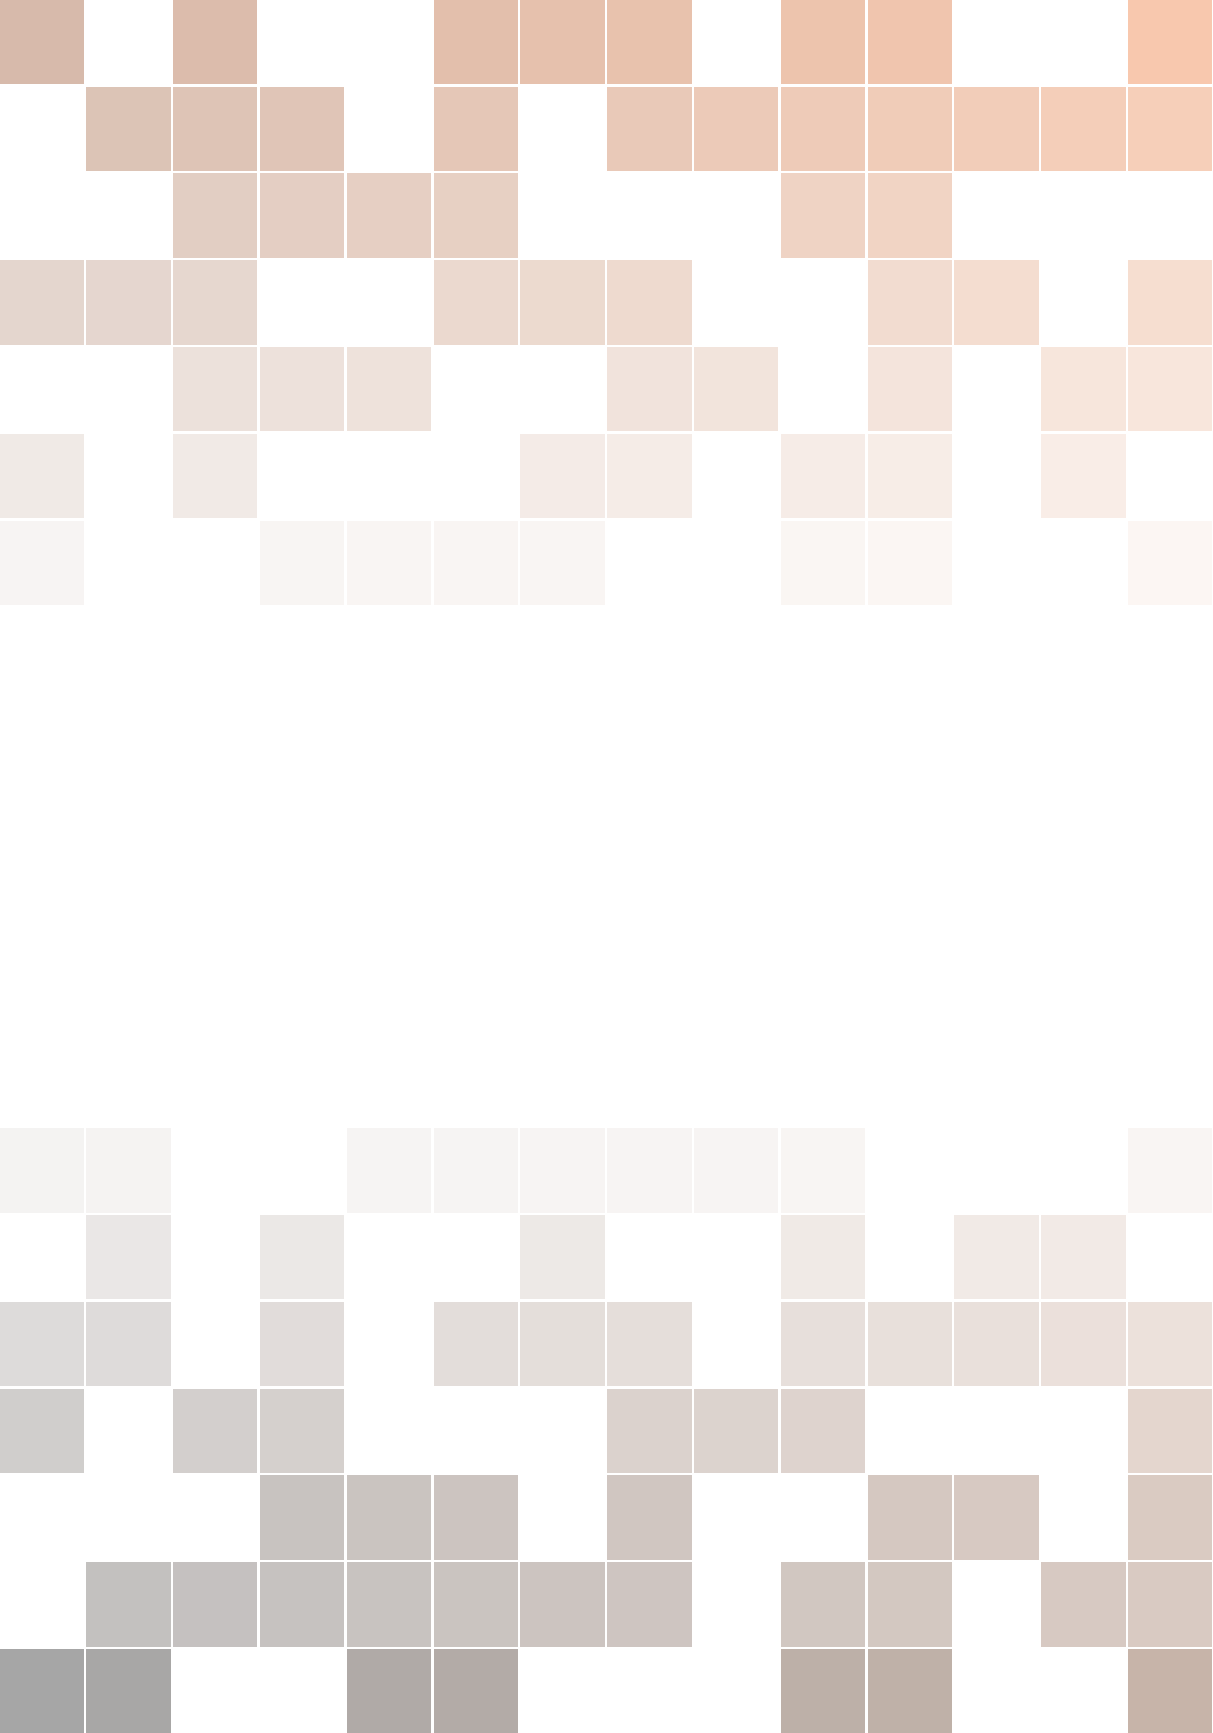
\includegraphics[width=\paperwidth]{background.pdf}};
\draw (current page.center) node [fill=ocre!30!white,fill opacity=0.6,text opacity=1,inner sep=1cm]{\Huge\centering\bfseries\sffamily\parbox[c][][t]{\paperwidth}{\centering Math Notes\\[15pt] % Book title
{\Large My English Note}\\[20pt] % Subtitle
{\huge Xia Wenxuan}}}; % Author name
\end{tikzpicture}
\vfill
\endgroup
\else
\ifdefined\printvocabulary
\begingroup
\thispagestyle{empty} % Suppress headers and footers on the title page
\begin{tikzpicture}[remember picture,overlay]
\node[inner sep=0pt] (background) at (current page.center) {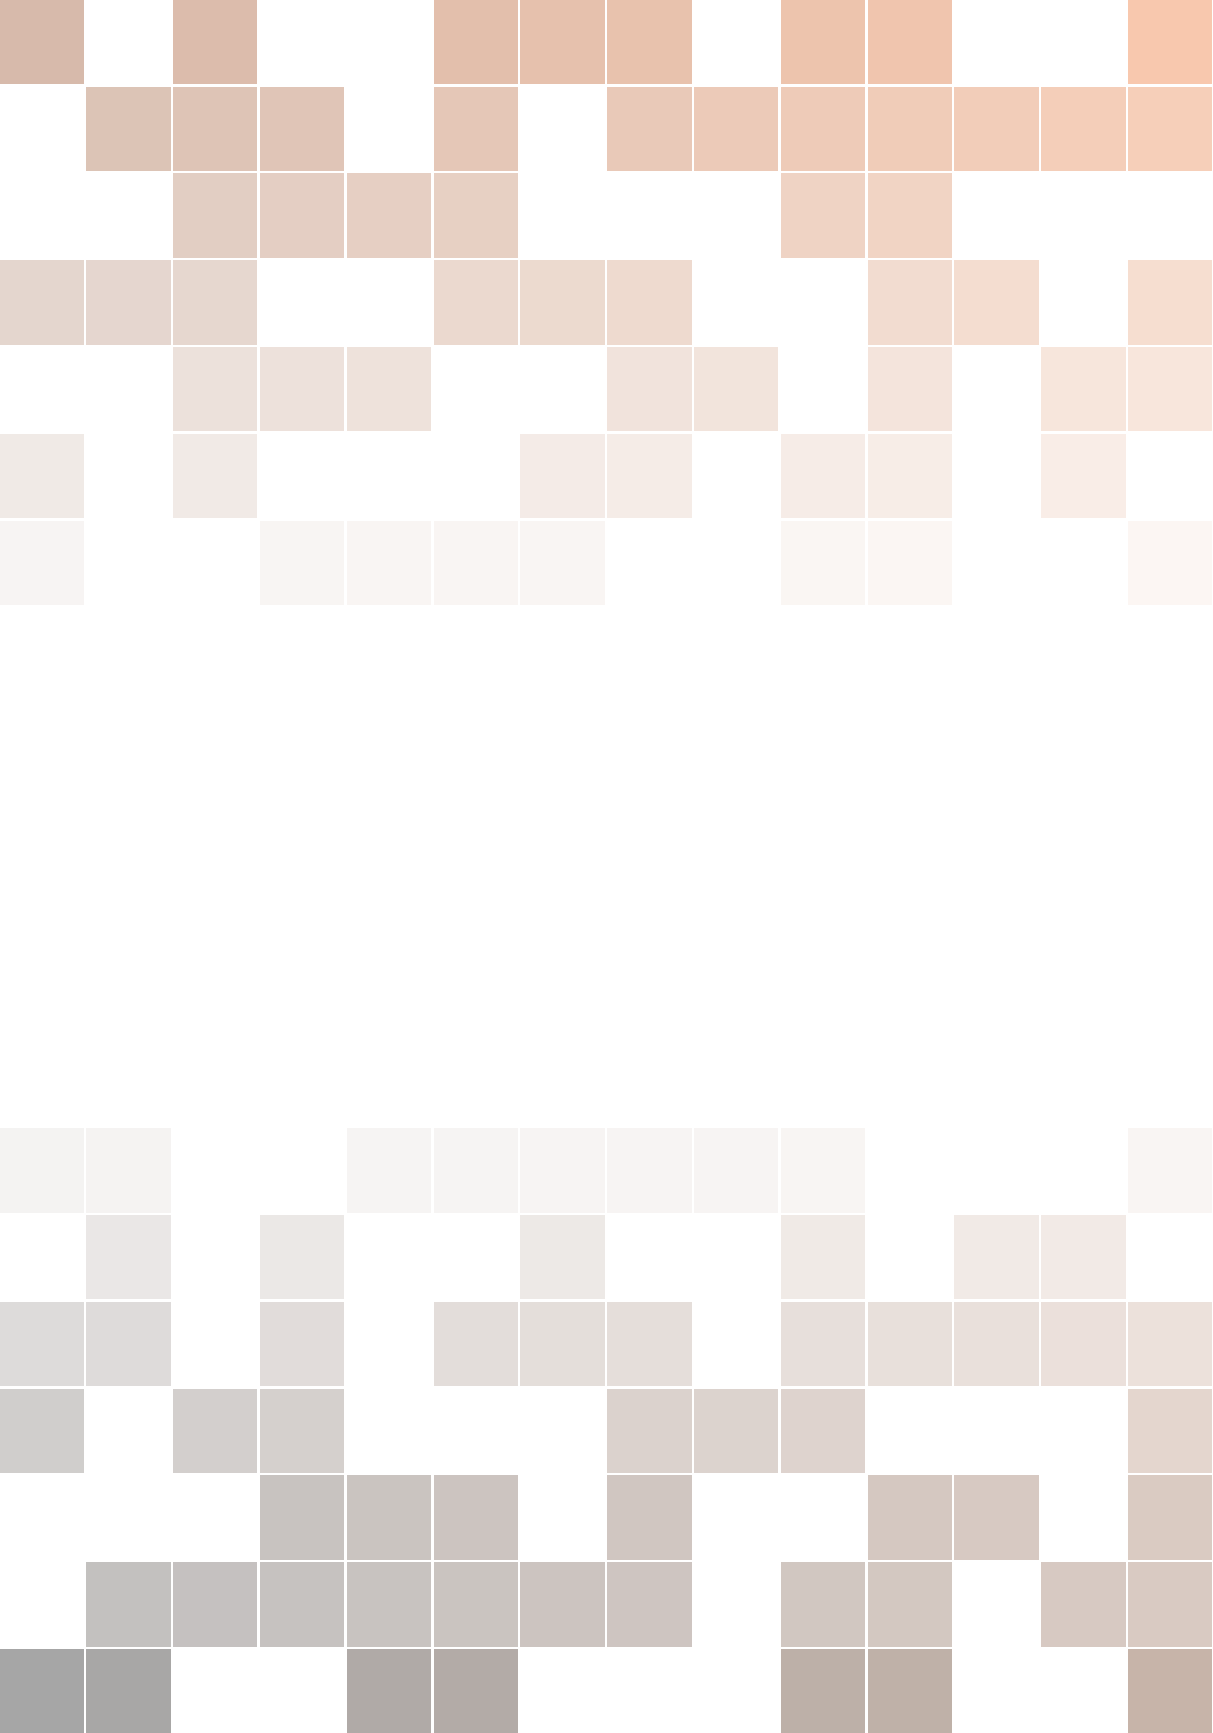
\includegraphics[width=\paperwidth]{background.pdf}};
\draw (current page.center) node [fill=ocre!30!white,fill opacity=0.6,text opacity=1,inner sep=1cm]{\Huge\centering\bfseries\sffamily\parbox[c][][t]{\paperwidth}{\centering The Beauty of Embracing English\\[15pt] % Book title
{\Large My English Note}\\[20pt] % Subtitle
{\huge Xia Wenxuan}}}; % Author name
\end{tikzpicture}
\vfill
\endgroup
\fi
\fi

%----------------------------------------------------------------------------------------
%	COPYRIGHT PAGE
%----------------------------------------------------------------------------------------

\newpage
~\vfill
\thispagestyle{empty}

% \noindent Copyright \copyright\ 2021 Xia Wenxuan\\ % Copyright notice
\noindent Written by Xia Wenxuan, 2021\\

\noindent \textsc{Published by myself}\\ % Publisher

\noindent \textsc{\url{https://github.com/gegeji}}\\ % URL

\noindent Licensed under the Creative Commons Attribution-NonCommercial 3.0 Unported License (the ``License''). You may not use this file except in compliance with the License. You may obtain a copy of the License at \url{http://creativecommons.org/licenses/by-nc/3.0}. Unless required by applicable law or agreed to in writing, software distributed under the License is distributed on an \textsc{``as is'' basis, without warranties or conditions of any kind}, either express or implied. See the License for the specific language governing permissions and limitations under the License.\\ % License information, replace this with your own license (if any)

\noindent All the material in this document is taken from my textbook or catechism video material, and some of it uses optical character recognition (OCR) to aid input. It may contain typographical or content inaccuracies. This document is for my personal study only. I am not responsible for the accuracy of the content of the text.\\

\noindent \textit{Edited and Revised on \today} % Printing/edition date

%----------------------------------------------------------------------------------------
%	TABLE OF CONTENTS
%----------------------------------------------------------------------------------------

%\usechapterimagefalse % If you don't want to include a chapter image, use this to toggle images off - it can be enabled later with \usechapterimagetrue

\chapterimage{chapter_head_3.png} % Table of contents heading image

\pagestyle{empty} % Disable headers and footers for the following pages

\tableofcontents % Print the table of contents itself

\cleardoublepage % Forces the first chapter to start on an odd page so it's on the right side of the book

\pagestyle{fancy} % Enable headers and footers again

% algorithm with a box
\RestyleAlgo{boxruled}
\LinesNumbered
%----------------------------------------------------------------------------------------
%	Main Body
%----------------------------------------------------------------------------------------




\ifdefined\printvocabulary

\part{All Roots}
% roots
\chapter{Hearing, Seeing, Saying, Doing}

\section{vis}
\begin{wordRef}{visual, visualize}[visual]
\end{wordRef}

\begin{wordRef}{visible, visibility, invisible}[visible]
\end{wordRef}

\section{audi- (声音)}
\begin{wordRef}{audio}
\end{wordRef}

\begin{wordRef}{audience}
\end{wordRef}

\begin{wordRef}{audition}
\end{wordRef}

\section{{ag- (做,加强)}}

\begin{wordRef}{agenda}
\end{wordRef}

\begin{wordRef}{agency}
\end{wordRef}

\begin{wordRef}{agent}
\end{wordRef}

\begin{wordRef}{aggress, aggressive, aggressor}[aggress]
\end{wordRef}

\section{dict (doing)}

\begin{wordRef}{predict, prediction, predictable, unpredictable}[predict]
\end{wordRef}

\begin{wordRef}{contradict, contradiction, contradictory}[contradict]
\end{wordRef}

\section{log (saying)}

\begin{wordRef}{dialogue}
\end{wordRef}

\begin{wordRef}{monologue}
\end{wordRef}

\begin{wordRef}{prologue}
\end{wordRef}

\begin{wordRef}{epilogue}
\end{wordRef}

\section{loqu (saying)}

\begin{wordRef}{eloquent, eloquence}[eloquent]
\end{wordRef}

\begin{wordRef}{loquacious}
\end{wordRef}
\chapter{Holding, Seizing, Following}

\section{prehand/pris}

\begin{RefWord}{comprehend, comprehension, comprehensible}[comprehend]
\end{RefWord}

\begin{RefWord}{comprehensive}
\end{RefWord}

\begin{RefWord}{apprehend, apprehension, apprehensive}[apprehend]
\end{RefWord}

\begin{RefWord}{surprise}
\end{RefWord}

\begin{RefWord}{comprise}
\end{RefWord}

\begin{RefWord}{enterprise, enterpriser}[enterprise]
\end{RefWord}

\begin{RefWord}{prison}
\end{RefWord}

\begin{RefWord}{imprison}
\end{RefWord}

\section{sequ/secut (following)}

\begin{RefWord}{sequence, sequential}[sequence]
\end{RefWord}

\begin{RefWord}{subsequent, subsequence}[subsequent]
\end{RefWord}

\begin{RefWord}{sequel}
\end{RefWord}

\begin{RefWord}{consequent, consequence}[consequent]
\end{RefWord}

\begin{RefWord}{execute, execution, executive}[execute]
\end{RefWord}

\begin{RefWord}{consecutive}
\end{RefWord}

\begin{RefWord}{prosecute, prosecution, prosecutor}[prosecute]
\end{RefWord}

\begin{RefWord}{presecute}
\end{RefWord}

\section{tain (握、持)}

\begin{RefWord}{maintain}
\end{RefWord}

\begin{RefWord}{obtain}
\end{RefWord}

\begin{RefWord}{attain, attainment}[attain]
\end{RefWord}

\begin{RefWord}{abstain}
\end{RefWord}

\begin{RefWord}{sustain, sustainable, sustainability}[sustain]
\end{RefWord}

\begin{RefWord}{detain, detainer, detainee, detainment}[detain]
\end{RefWord}

\begin{RefWord}{retain}
\end{RefWord}
\chapter{Feet, Running, Walking}

\section{cede, ceed, cess (走)}

\begin{RefWord}{exceed, excess, excessive, excessively}[exceed]
\end{RefWord}

\begin{RefWord}{proceed}
\end{RefWord}

\begin{RefWord}{precede, preceding, precedence}[precede]
\end{RefWord}

\begin{RefWord}{succession}
\end{RefWord}

\begin{RefWord}{successor}
\end{RefWord}

\begin{RefWord}{aggress, aggressive, aggressor}[aggress]
\end{RefWord}

\section{grad (walking)}

\begin{RefWord}{graduate}
\end{RefWord}

\begin{RefWord}{gradual}
\end{RefWord}

\begin{RefWord}{gradually}
\end{RefWord}

\begin{RefWord}{upgrade}
\end{RefWord}

\section{gress (walk)}

\begin{RefWord}{progress}
\end{RefWord}

\begin{RefWord}{aggress, aggressive, aggressor}[aggress]
\end{RefWord}

\section{ambul, ambl (walking)}
\begin{RefWord}{ambulance}
\end{RefWord}

\begin{RefWord}{ambulate}
\end{RefWord}

\begin{RefWord}{ambulant}
\end{RefWord}

\begin{RefWord}{preamble}
\end{RefWord}

\section{cur, curs, cours (to run)}

\begin{RefWord}{occur, occurence}[occur]
\end{RefWord}

\begin{RefWord}{excursion, excurse}[excursion]
\end{RefWord}


\begin{RefWord}{concur}
    
\end{RefWord}

\begin{RefWord}{concurrent, concurrency}[concurrent]
\end{RefWord}

\begin{RefWord}{course}
\end{RefWord}

\section{pass (to walk through)}

\begin{RefWord}{pass}
\end{RefWord}

\begin{RefWord}{compass}
\end{RefWord}

\begin{RefWord}{passage}
\end{RefWord}

\begin{RefWord}{passenger}
\end{RefWord}

\begin{RefWord}{trespass}
\end{RefWord}

\section{ped (feet)}

\begin{RefWord}{pedal}
\end{RefWord}

\begin{RefWord}{impede, impediment}[impede]
\end{RefWord}

\begin{RefWord}{expedite}
\end{RefWord}

\begin{RefWord}{expedition}
\end{RefWord}

\section{vad}

\begin{RefWord}{invade}
\end{RefWord}

\begin{RefWord}{evade, evasion, evasive, evasively, evasiveness}[evade]
\end{RefWord}

\begin{RefWord}{pervade}
\end{RefWord}

\begin{RefWord}{lavender}
\end{RefWord}
\chapter{Dragging, Cutting, Parting}

\section{part}

\begin{RefWord}{department}
\end{RefWord}

\begin{RefWord}{depart, departure}[depart]
\end{RefWord}

\begin{RefWord}{apartment}
\end{RefWord}

\begin{RefWord}{apart}
\end{RefWord}

\begin{remark}
    apartment 在主要含义上不是 apart 的名词形式. 
\end{remark}

\begin{RefWord}{counterpart}
\end{RefWord}

\begin{RefWord}{partial, impartial, partially, partialness}[partial]
\end{RefWord}

\begin{RefWord}{partner}
\end{RefWord}

\begin{RefWord}{particular, particularly}[particular]
\end{RefWord}

\begin{RefWord}{participate, participation, participator}[participate]
\end{RefWord}

\begin{RefWord}{partake, partaker}[partake]
\end{RefWord}

\begin{RefWord}{partition}
\end{RefWord}

\begin{RefWord}{impart, impartment, imparter}[impart]
\end{RefWord}

\section{port}

\begin{RefWord}{proportion, proportional}[proportion]
\end{RefWord}

\begin{RefWord}{apportion}
\end{RefWord}

\begin{RefWord}{portion}
\end{RefWord}

\section{sect (to cut/to divide)}

\begin{RefWord}{section}
\end{RefWord}

\begin{RefWord}{insect}
\end{RefWord}

\begin{RefWord}{insectcide}
\end{RefWord}

\begin{RefWord}{bisect}
\end{RefWord}

\begin{RefWord}{dissect, dissection. dissectible}[dissect]
\end{RefWord}

\begin{RefWord}{intersect, intersection}[intersect]
\end{RefWord}

\begin{RefWord}{segment, segmentation, segmental}[segment]
\end{RefWord}

\section{tract (to draw/to drag)}

\begin{RefWord}{tractor}
\end{RefWord}

\begin{RefWord}{traction}
\end{RefWord}

\begin{RefWord}{attract, attraction, attractive}[attract]
\end{RefWord}

\begin{RefWord}{distract, dictracting, distracted, distraction}[distract]
\end{RefWord}

\begin{RefWord}{contract, contraction}[contract]
\end{RefWord}

\begin{RefWord}{extract, extraction, extractor}[extract]
\end{RefWord}

\begin{RefWord}{abstract, abstraction, abstractly}[abstract]
\end{RefWord}

\begin{RefWord}{detract, detraction}[detract]
\end{RefWord}

\begin{RefWord}{protract} 
\end{RefWord}

\begin{RefWord}{retract, retractable}[retract]
\end{RefWord}

\begin{RefWord}{subtract, subtraction, subtractive}[subtract]
\end{RefWord}

\section{cide/cise (cutting)}

\begin{RefWord}{decide}
\end{RefWord}

\begin{RefWord}{suicide}
\end{RefWord}

\begin{RefWord}{insecticide}
\end{RefWord}

\begin{RefWord}{pesticide}
\end{RefWord}

\begin{RefWord}{concise}
\end{RefWord}

\begin{RefWord}{precise}
\end{RefWord}

\begin{RefWord}{excise}
\end{RefWord}

\begin{RefWord}{incise}
\end{RefWord}

\begin{RefWord}{incisor}
\end{RefWord}





\chapter{Turning, Rolling and Pushing}

\section{pel (pushing)}

\begin{wordRef}{repel, repulsive}[repel]
\end{wordRef}

\begin{wordRef}{impel}
\end{wordRef}

\begin{wordRef}{compel,  compulsion}[compel]
\end{wordRef}

\begin{wordRef}{propel}
 \end{wordRef}


\begin{wordRef}{propeller}
\end{wordRef}

\begin{wordRef}{dispel}
\end{wordRef}

\begin{wordRef}{expel, expulsion}[expel]
\end{wordRef}

\begin{wordRef}{compel}
\end{wordRef}



\section{vert (turn and rolling)}

\begin{wordRef}{revert, reverse}[revert]
\end{wordRef}

\begin{wordRef}{convert}
\end{wordRef}

\begin{wordRef}{subvert}
\end{wordRef}

\begin{wordRef}{convert, convertible}[convert]
\end{wordRef}

\begin{wordRef}{subvert, subversion}[subvert]
\end{wordRef}

\begin{wordRef}{diverse, diversify}[diverse]
\end{wordRef}

\begin{wordRef}{avert}
\end{wordRef}

\begin{wordRef}{adversity}
\end{wordRef}

\begin{wordRef}{pervert}
\end{wordRef}

\begin{wordRef}{divert, diversion, diverting}[divert]
\end{wordRef}

\begin{wordRef}{controversial, controversially, controversy}[controversial]
\end{wordRef}

\begin{wordRef}{introvert}
\end{wordRef}

\section{volv (turn and rolling)}



\begin{wordRef}{devolve}
\end{wordRef}


\begin{wordRef}{VOLVE}
\end{wordRef}

\begin{wordRef}{revolve, revolving, revolution}[revolve]
\end{wordRef}


\chapter{Looking, Breathing and Calling}

\section{spect}

\begin{wordRef}{spectator}
\end{wordRef}

\begin{wordRef}{expect}
\end{wordRef}

\begin{wordRef}{respect}
\end{wordRef}

\begin{wordRef}{aspect}
\end{wordRef}

\begin{wordRef}{inspect}
\end{wordRef}

\begin{wordRef}{suspect}
\end{wordRef}

\begin{wordRef}{perspective}
\end{wordRef}

\begin{wordRef}{prospect, prospective}[prospect]
\end{wordRef}

\begin{wordRef}{introspect}
\end{wordRef}

\begin{wordRef}{introspective}
\end{wordRef}

\begin{wordRef}{spectrum}
\end{wordRef}

\begin{wordRef}{circumspect}
\end{wordRef}

\begin{wordRef}{retrospect, retrospective}[retrospect]
\end{wordRef}

\begin{wordRef}{retrospective}
\end{wordRef}

\begin{wordRef}{spectacle}
\end{wordRef}

\begin{wordRef}{spectacular}
    a mountainous area with spectacular scenery

    very sudden, unexpected, or extreme
    \textit{The news caused a spectacular fall in the stock market. 这一消息引起了股市的暴跌。}
\end{wordRef}


















\section{spir (to breatge)}





\begin{wordRef}{inspire, inspiration, inspiring, inspirational}[inspire]
\end{wordRef}

\begin{wordRef}{aspire, aspiration}[aspire]
\end{wordRef}

\begin{wordRef}{perspire, perspiration}[perspire]
\end{wordRef}

\begin{wordRef}{conspire, conspiracy}[conspire]
\end{wordRef}

\begin{wordRef}{expire, expiration}[expire]
\end{wordRef}

\begin{wordRef}{respire, respiratory, respiration}[respire]
\end{wordRef}


\section{hal (breathe)}

\begin{wordRef}{exhale}
\end{wordRef}

\begin{wordRef}{inhale}
\end{wordRef}




\section{voc, vok, claim}

\part{Other Roots}
\chapter{Other Roots}

\section{a (加强)}

\begin{RefWord}{aspire}
\end{RefWord}

\section{ac (加强)}

\begin{RefWord}{acclaim}
\end{RefWord}

\section{ap}

\begin{RefWord}{apportion, apportionment}[apportion]
\end{RefWord}

\section{anti}

\begin{RefWord}{antibiotics}
\end{RefWord}

\section{ate (give)}

\begin{RefWord}{animate}
\end{RefWord}

\begin{RefWord}{desperate}
\end{RefWord}

\begin{RefWord}{terminate}
\end{RefWord}



\begin{RefWord}{exterminate}
\end{RefWord}

\section{bi (两个)}

\begin{RefWord}{binary}
\end{RefWord}

\begin{RefWord}{bisect}
\end{RefWord}

\section{cide}

\begin{RefWord}{insectcide}
\end{RefWord}

\section{com (共同)}

\begin{RefWord}{compass}
\end{RefWord}

\begin{RefWord}{compel}
\end{RefWord}

\begin{RefWord}{compromise}
\end{RefWord}

\begin{RefWord}{commit, commitment}[commit]
\end{RefWord}

\begin{RefWord}{combat}
\end{RefWord}

\section{con (共同; 全部; inside out)}
\begin{RefWord}{concur}
\end{RefWord}

\begin{RefWord}{concurrent}
\end{RefWord}

\begin{RefWord}{contract}
\end{RefWord}

\begin{RefWord}{concise}
\end{RefWord}

\begin{RefWord}{convert}
\end{RefWord}

\begin{RefWord}{conspire, conspiracy}[conspire]
\end{RefWord}

\begin{RefWord}{conduct}
\end{RefWord}

\begin{RefWord}{contact}
\end{RefWord}

\section{contra (opposite)}

\begin{RefWord}{contradict, contradiction, contradictory}[contradict]
\end{RefWord}

\section{counter}

\begin{RefWord}{counterpart}
\end{RefWord}

\section{de (向下; 加强; 使得; 剥夺)}

\begin{RefWord}{detract}
\end{RefWord}

\begin{RefWord}{depart}
\end{RefWord}

\begin{RefWord}{decide}
\end{RefWord}

\begin{RefWord}{devolve}
\end{RefWord}

\begin{RefWord}{detrimental}
    causing harm or damage (harmful, damaging)
\end{RefWord}

\begin{RefWord}{deter}
\end{RefWord}

\begin{RefWord}{desperate, desperately, desperation, desperado}
\end{RefWord}

\begin{RefWord}{despair}
\end{RefWord}

\begin{RefWord}{deject, dejection}[deject]
\end{RefWord}

\begin{RefWord}{deduce, deducible, deductive, deduction}[deduce]
\end{RefWord}

\begin{RefWord}{debate}
\end{RefWord}

\begin{RefWord}{determine}
\end{RefWord}

\section{dis (separate; out)}

\begin{RefWord}{disconnect}
\end{RefWord}

\begin{RefWord}{distract, dictracting, distracted, distraction}[distract]
\end{RefWord}

\begin{RefWord}{disproportion, disproportional}[proportion]
\end{RefWord}

\begin{RefWord}{dispel}
\end{RefWord}

\begin{RefWord}{disclaim}
\end{RefWord}

\begin{RefWord}{dismiss, dismissal}[dismiss]
\end{RefWord}

\begin{RefWord}{disturb}
    dis 全面的
\end{RefWord}


\section{e (forward, 加强)}

\begin{RefWord}{evolve}
\end{RefWord}

\begin{RefWord}{evoke, evocation, evocable}[evoke]
\end{RefWord}

\begin{RefWord}{eject, ejection}[eject]
\end{RefWord}

\section{-ent (person)}

\begin{RefWord}{agent}
\end{RefWord}

\section{er (person)}

\begin{RefWord}{partner}
\end{RefWord}

\begin{RefWord}{partaker}[partake]
\end{RefWord}

\begin{RefWord}{imparter}
\end{RefWord}

\begin{RefWord}{employer}
\end{RefWord}

\begin{RefWord}{employee}
\end{RefWord}

\begin{RefWord}{producer}[produce]
\end{RefWord}

\section{ex (出去; 向外)}

\begin{RefWord}{excessive}[excess]
\end{RefWord}

\begin{RefWord}{exchange}
\end{RefWord}

\begin{RefWord}{ex-boyfriend}
\end{RefWord}

\begin{RefWord}{external}
\end{RefWord}

\begin{RefWord}{excurse, excursion}[excurse]
\end{RefWord}

\begin{RefWord}{extract}
\end{RefWord}

\begin{RefWord}{excise}
\end{RefWord}

\begin{RefWord}{expel}
    Syn $\rightarrow$ (dispel) \ref{dispel}.
\end{RefWord}

\begin{RefWord}{expire, expiration}[expire]
\end{RefWord}

\begin{RefWord}{exhale}
\end{RefWord}

\begin{RefWord}{exclaim, exclaimation}[exclaim]
\end{RefWord}

\begin{RefWord}{exterminate}
\end{RefWord}

\section{graphy (to write)}

\begin{RefWord}{biography, biographer}[biography]
\end{RefWord}

\begin{RefWord}{typography}
\end{RefWord}

\begin{RefWord}{geography}
\end{RefWord}

\begin{RefWord}{photography, photograph, photographer}[photograph]
\end{RefWord}


\section{impart (进入……里面)}
\begin{RefWord}{impart, imparter}[impart]
\end{RefWord}

\section{in}

\begin{RefWord}{inside}
\end{RefWord}

\begin{RefWord}{invade}
\end{RefWord}

\begin{RefWord}{inhale}
\end{RefWord}

\begin{RefWord}{invigorate}
\end{RefWord}

\begin{RefWord}{inject, injection}[inject]
\end{RefWord}

\begin{RefWord}{induce, inducement}[induce]
\end{RefWord}

\begin{RefWord}{indocile}[docile]
\end{RefWord}

\begin{RefWord}{interminable}
\end{RefWord}

\section{inter (在中间)}

\begin{RefWord}{intersect}
\end{RefWord}

\section{introspect}

\begin{RefWord}{introspect}
\end{RefWord}

\section{ir} 

\begin{RefWord}{irregular}
\end{RefWord}

\begin{RefWord}{irrevocable}
\end{RefWord}

\begin{RefWord}{irresponsible}
\end{RefWord}

\begin{RefWord}{irrelevant}
\end{RefWord}

\section{ist}

\begin{RefWord}{imperialist}
\end{RefWord}

\begin{RefWord}{vocalist}[vocal]
\end{RefWord}

\section{ment}

\begin{RefWord}{department}
\end{RefWord}

\begin{RefWord}{apartment}
\end{RefWord}

\begin{RefWord}{impartment}[impart]
\end{RefWord}

\section{mis}

\begin{RefWord}{misconduct}
\end{RefWord}

\begin{RefWord}{misconception}
\end{RefWord}

\begin{RefWord}{misfortune}
\end{RefWord}

\begin{RefWord}{mislead}
\end{RefWord}

\begin{RefWord}{misinterpret}
\end{RefWord}

\section{oc (toward)}

\begin{RefWord}{occur}
\end{RefWord}

\section{or (人)}


\begin{RefWord}{doctor}
\end{RefWord}

\begin{RefWord}{aggressor}[aggress]
\end{RefWord}

\begin{RefWord}{tractor}
\end{RefWord}

\begin{RefWord}{contractor}
\end{RefWord}

\begin{RefWord}{monitor}
\end{RefWord}

\begin{RefWord}{extractor}
\end{RefWord}

\begin{RefWord}{detractor}
\end{RefWord}

\begin{RefWord}{participate, participation, participator}[participate]
\end{RefWord}

\begin{RefWord}{incisor}
\end{RefWord}

\begin{RefWord}{spectator}
\end{RefWord}

\begin{RefWord}{terror}
\end{RefWord}

\begin{RefWord}{horror}
\end{RefWord}

\begin{RefWord}{abductor, abductee}[abduct]
\end{RefWord}

\begin{RefWord}{terminator}[terminate]
\end{RefWord}

\begin{RefWord}{exterminator}[exterminate]
\end{RefWord}

\section{orium}

\begin{RefWord}{auditorium}
\end{RefWord}

\section{per (穿过)}
{per- (穿过)}

\begin{RefWord}{pervade}
\end{RefWord}

\begin{RefWord}{perspective}
\end{RefWord}

\begin{RefWord}{perspire}
\end{RefWord}

\section{pre (before)}
\begin{RefWord}{precede}
\end{RefWord}

\begin{RefWord}{previous}
\end{RefWord}

\begin{RefWord}{predict, prediction, predictable, unpredictable}[predict]
\end{RefWord}

\begin{RefWord}{precise}
\end{RefWord}

\section{pro- (moving forward)}

\begin{RefWord}{proceed}
\end{RefWord}

\begin{RefWord}{progress}
\end{RefWord}

\begin{RefWord}{protract}
\end{RefWord}

\begin{RefWord}{propel}
\end{RefWord}

\begin{RefWord}{propeller}
\end{RefWord}

\begin{RefWord}{prospect}
\end{RefWord}

\begin{RefWord}{provoke}
\end{RefWord}

\begin{RefWord}{proclaim}
\end{RefWord}

\begin{RefWord}{project, projection}[project]
\end{RefWord}

\begin{RefWord}{compromise}
\end{RefWord}

\section{re (again, back, 否认, 向相反方向)}

\begin{RefWord}{revolve}
\end{RefWord}

\begin{RefWord}{revert}
\end{RefWord}

\begin{RefWord}{rebel}
\end{RefWord}

\begin{RefWord}{revolt}
\end{RefWord}

\begin{RefWord}{revolution, revolutionary, revolutionize}[revolve]
\end{RefWord}

\begin{RefWord}{respire}
\end{RefWord}

\begin{RefWord}{revoke}
\end{RefWord}

\begin{RefWord}{reclaim}
\end{RefWord}

\begin{RefWord}{reject}
\end{RefWord}

\begin{RefWord}{recreate, recreation}[recreate]
\end{RefWord}

\begin{RefWord}{reproduce}
\end{RefWord}

\begin{RefWord}{repeat}
\end{RefWord}

\begin{RefWord}{reduce}
\end{RefWord}

\begin{RefWord}{rebate}
\end{RefWord}

\section{retro (向后, 倒退)}
\begin{RefWord}{retrospect}
\end{RefWord}

\section{se (sex)}

\begin{RefWord}{sex}
\end{RefWord}

\begin{RefWord}{seduce, seduction}[seduce]
\end{RefWord}


\section{sub (向下)}

\begin{RefWord}{subtract}
\end{RefWord}

\begin{RefWord}{subvert}
\end{RefWord}

\begin{RefWord}{subconscious, subconsciously}
\end{RefWord}

\begin{RefWord}{subjective}
\end{RefWord}

\section{sus}

\begin{RefWord}{suspect, suspicion}
\end{RefWord}

\begin{RefWord}{susceptible}
\end{RefWord}

\begin{RefWord}{suspend, suspension}
\end{RefWord}

\section{-sm}

\begin{RefWord}{imperialism}
\end{RefWord}

\section{sphere}
\begin{RefWord}{biosphere}
\end{RefWord}

\begin{RefWord}{hemisphere}
\end{RefWord}

\begin{RefWord}{atmosphere}
\end{RefWord}

\section{tion}

\begin{RefWord}{detraction}[detract]
\end{RefWord}

\section{tail}



\section{tran-}

\begin{RefWord}{transcipt}
    written copy of a speech
\end{RefWord}

\begin{RefWord}{transribe}
\end{RefWord}

\begin{RefWord}{transfer}
\end{RefWord}

\begin{RefWord}{transform}
\end{RefWord}

\begin{RefWord}{transformer}
\end{RefWord}

\begin{RefWord}{transit, transition}[transit]
\end{RefWord}

\begin{RefWord}{transmit, transmission}[transmit]
\end{RefWord}

\begin{RefWord}{tranplant}
\end{RefWord}

\begin{RefWord}{transport, transportation}[transport]
\end{RefWord}

\section{tres (横穿)}

\begin{RefWord}{trespass}
\end{RefWord}

\part{All Words}
% all words



\chapter{A - G}
\section{A, a}

\begin{DefWord}{agenda}
\end{DefWord}

\begin{DefWord}{agency}
\end{DefWord}

\begin{DefWord}{agent}
\end{DefWord}

\begin{DefWord}{aggress, aggressive, aggressor}[aggress]
\end{DefWord}

\begin{DefWord}{ambulance}
\end{DefWord}

\begin{DefWord}{ambulate} 
    ambulate /ˈæm byəˌleɪt/
    
    to walk about or move from place to place.
\end{DefWord}

\begin{DefWord}{ambulant} 
    ambulant /ˈæmbjələnt/
    
    (of a patient) able to walk; not having to stay in bed
\end{DefWord}

\begin{DefWord}{audio}
\end{DefWord}

\begin{DefWord}{audience}
\end{DefWord}

\begin{DefWord}{audition} 
    My  niece  was admitted  to  the Juilliard School of Music  in  America. But before that she was asked to attend an audition.
\end{DefWord}

\begin{DefWord}{auditorium}
\end{DefWord}

\begin{DefWord}{audible, inaudible}[audible]
    The audio-visual equipment there  is  magnificent that even  in the  farthest seat the music is still audible.
\end{DefWord}


\begin{DefWord}{aggress, aggressive, aggressor}[aggress]
\end{DefWord}

\begin{DefWord}{agent}
\end{DefWord}

\begin{DefWord}{apartment}
    a set of rooms on one floor of a large building, where someone lives

    a room or set of rooms used by an important person such as a president
    \textit{ I had never been in the prince's private apartments before.}
\end{DefWord}

\begin{DefWord}{apart}
    \textit{two miles/six feet etc apart}
    \textit{two days/three weeks/five years etc apart}

    if something comes apart, or you take it apart, it is separated into different pieces
    \textit{The whole thing \textbf{comes apart} so that you can clean it.}
    \textit{They \textbf{took} the engine \textbf{apart} to see what was wrong.}

    if you keep things apart, you keep them separate from each other
    \textit{I try to \textbf{keep} my work and private life as far \textbf{apart} as possible.}

    if people are apart, they are not together in the same place, or not having a relationship with each other
    \textit{The children have never been apart before.}

    \textbf{fall apart}
    if something falls apart, it breaks into different pieces;
    if something is falling apart, it is in very bad condition
    \textit{He drives around in an old car that's falling apart.}

    \textbf{be torn apart} if a marriage, family etc is torn apart, it can no longer continue because of serious difficulties
    \textit{The play portrays a good marriage torn apart by external forces.}

    \textbf{be worlds/poles apart} if people, beliefs, or ideas are worlds or poles apart, they are completely different from each other
    \textit{I realized we were still worlds apart. 我意识到我们之间仍有天壤之别. }

    \textbf{grow/drift apart} if people drift or grow apart, their relationship slowly becomes less close
    \textit{Lewis and his father drifted apart after he moved to New York.}

    \textbf{joking apart} used to say that you want to say something
    seriously

    \textbf{somebody/something apart} except for someone or something
    \textit{The car industry apart, most industries are now seeing an improvement in their economic performance.}

    \textbf{set somebody/something apart} to make someone or something different from other people or things
    \textit{Her unusual lifestyle set her apart as a child.}
\end{DefWord}

\begin{DefWord}{apportion, apportionment}[apportion]
    to decide how something should be shared among various people

    \textit{It's not easy to \textbf{apportion blame} (=say who deserves to be blamed) when a marriage breaks up.}
    \textit{Court costs were equally apportioned between them.}
\end{DefWord}

\begin{DefWord}{apprehend, apprehension, apprehensive}[apprehend]
    arrest (someone) for a crime.
    $\star$"\textit{a warrant was issued but he has not been apprehended}";
    
    (old-fashioned) understand or perceive.
    "\textit{great art invites us to apprehend beauty}";to be apprehensive, suspicious, or fearful; fear.

    apprehensive: 担心 We'd been a little {apprehensive} about their visit.
\end{DefWord}

\begin{DefWord}{attain, attainment}[attain]
    sense of attainment
\end{DefWord}

\begin{DefWord}{abstain}
    抑制
    e.g. \textit{The man tries so hard to abstain from drinking.}
    
    戒绝, 弃权
    e.g. \textit{When you are in China, will you have to abstain from voting in your country?}
    \textit{Pilots must abstain from alcohol for 24 hours before flying.}
\end{DefWord}

\begin{DefWord}{abstract, abstraction, abstractly}[abstract]
    based on general ideas or principles rather than specific examples or real events (syn theoretical)

    existing only as an idea or quality rather than as something real that you can see or touch (opp concerte)

    a painting, design etc which contains shapes or images that do not look like real things or people抽象画;抽象设计;抽象派作品

    a short written statement containing only the most important ideas in a speech, article etc
    
    \textbf{in the abstract} considered in a general way rather than being based on specific details and examples

    to write a document containing the most important ideas or points from a speech, article etc

    (formal) to remove something from somewhere
\end{DefWord}

\begin{DefWord}{attract, attraction, attractive}[attract]
\end{DefWord}

\begin{DefWord}{avert}
    to prevent something unpleasant from happening
    \textit{The tragedy could have been averted if the crew had followed safety procedures.}

    \textbf{avert your eyes/gaze etc} 
    to look away from something so that you do not see it
    \textit{Henry averted his eyes as she undressed.}

\end{DefWord}

\begin{DefWord}{adversity}
    a situation in which you have a lot of problems that seem to be caused by bad luck
    \textit{his courage in the face of adversity}
\end{DefWord}

\begin{DefWord}{adversary}
    a country or person you are fighting or competing against 对手,敌手 (SYN opponent)
\end{DefWord}

\begin{DefWord}{aspire}
    to desire and work towards achieving something important
    追求,渴望,有志于

    \textbf{aspire to}
    \textit{college graduates aspiring to careers in finance}

    \textbf{aspire to do something}
    \textit{At that time, all serious artists aspired to go to Rome.}
\end{DefWord}

\begin{DefWord}{advocate}
    to publicly support a particular way of doing something
    \textit{Those who advocate for doctor-assisted suicide say the terminally ill should not have to suffer.}

    someone who publicly supports someone or something
    \textit{She's a passionate advocate of natural childbirth.}
\end{DefWord}

\begin{DefWord}{acclaim, acclaimation}[acclaim]
    to praise someone or something publicly
\end{DefWord}
\section{B, b}

\begin{DefWord}{binary}
\end{DefWord}

\begin{DefWord}{bisect}
    to divide something into two equal parts
\end{DefWord}

\begin{DefWord}{biography, biographer}[biography]
    a book that tells what has happened in someone's life, written by someone else
\end{DefWord}

\begin{DefWord}{biocide}
    n. [微] 灭微生物剂;生物性农药(biocide的复数)
\end{DefWord}

\begin{DefWord}{biochemical}
\end{DefWord}

\begin{DefWord}{biodiversity}
\end{DefWord}
\section{C, c}

\begin{DefWord}{concur}
    to agree with someone or have the same opinion as them
    \textit{The committee largely concurred with these views.}
\end{DefWord}

\begin{DefWord}{concurrent, concurrency}[concurrent]
    existing or happening at the same time
    \textit{The exhibition reflected concurrent developments abroad.}
    concurrent with
    \textit{My opinions are concurrent with yours.}
\end{DefWord}

\begin{DefWord}{course}
    if a liquid or electricity courses somewhere, it flows there quickly
    \textit{Tears coursed down his cheeks.}

    if a feeling courses through you, you feel it suddenly and strongly
    \textit{His smile sent waves of excitement coursing through her.}

    a period of time or process during which something happens
    \textit{During the course of our conversation, it emerged that Bob had been in prison.}

    take/run its course: the usual or natural way that something changes, develops, or is done
    \textit{It seems the boom in World Music has run its course.}
\end{DefWord}

\begin{DefWord}{contradict, contradiction, contradictory}[contradict]
\end{DefWord}

\begin{DefWord}{contractor}
    See \ref{contract}.

    a person or company that agrees to do work or provide goods for another company
\end{DefWord}


\begin{DefWord}{counterpart}
    someone or something that has the same job or purpose as someone or something else in a different place
    \textit{Belgian officials are discussing this with their French counterparts.}
\end{DefWord}

\begin{DefWord}{compass}
\end{DefWord}

\begin{DefWord}{comprehend, comprehension, comprehensible}[comprehend]
    comprehensible input
\end{DefWord}

\begin{DefWord}{comprehensive}
    comprehensive introduction
\end{DefWord}

\begin{DefWord}{comprise}
    \textit{The house \textbf{comprises} two bedrooms, a kitchen, and a living room.} 
    
    \textit{The committee \textbf{is comprised of} well-known mountaineers. }
    
    \textit{Women \textbf{comprise} a high proportion of part-time workers.} 
    
    \textit{Food exports are very important, \textbf{comprising} 74\% of the total.}
\end{DefWord}

\begin{DefWord}{consequent, consequence}[consequent]
    something that happens as a result of a particular action or set of conditions; 
    
    (\textit{rare}) people of consequence; 
    
    \textbf{of little/no/any etc consequence} formal not very important or valuable
\end{DefWord}

\begin{DefWord}{consecutive}
   \textit{ It had rained for four consecutive days.}

    \textit{Can they win the title for the third consecutive season?}
\end{DefWord}

\begin{DefWord}{contract, contraction}[contract]
    /ˈkɒntrækt/ noun, /kənˈtrækt/ verb

    an official agreement between two or more people, stating what each will do

    \textbf{contract with/between}
    \textit{Tyler has agreed a seven-year contract with a Hollywood studio.}

    \textbf{contract to do sth}
    \textit{a three-year contract to provide pay telephones at local restaurants}

    \textbf{on a contract/under contract}
    \textit{Employees who refuse to relocate are in breach of contract} (=have done something not allowed by their contracts).


    \textbf{subject to contract}: if an agreement is subject to contract, it has not yet been agreed formally by a contract

    to become smaller or narrower
    \textit{Metal contracts as it cools.}

    to get an illness
    \textit{Two-thirds of the adult population there have contracted AIDS.}

    contraction: a very strong and painful movement of a muscle, especially the muscles around the womb (the part of a woman's or female animal's body where her baby grows before it is born 子宫 SYN  uterus) during birth
\end{DefWord}

\begin{DefWord}{concise, concisely, conciseness}[concise] 
\end{DefWord}

\begin{DefWord}{compel,  compulsion}[compel]
    to force someone to do something:
    \textit{The law will compel employers to provide health insurance.}

    (formal) to make people have a particular feeling or attitude
    \textit{His performance compelled the audience's attention.}
\end{DefWord}

\begin{DefWord}{convert, convertible}[convert]
    to change something into a different form, or to change something so that it can be used for a different purpose or in a different way

    convert sth to/into sth
    \textit{They converted the spare bedroom into an office.}

    \textit{a 19th-century \textbf{converted barn}} (=barn changed into a house)

    to change into a different form, or change into something that can be used for a different purpose or in a different way 改建;改装;改造;转换

    \textbf{convert to/into}
    to persuade someone to change to a different religion
    \textit{convert somebody to something
    European missionaries converted thousands to Christianity. 欧洲的传教士使成千上万的人皈依了基督教. }

    to change to a different set of ideas, principles, or ways of doing something
    \textit{people who have recently converted to vegetarianism}
\end{DefWord}

\begin{DefWord}{controversial, controversially, controversy}[controversial]
\end{DefWord}

\begin{DefWord}{circumspect}
    thinking carefully about something before doing it, in order to avoid risk (cautious)
\end{DefWord}

\begin{DefWord}{conspire, conspiracy}[conspire]
    conspiracy /kənˈspɪrəsi/

    to secretly plan with someone else to do something illegal

    \textbf{conspire (with somebody) to do something}
    \textit{All six men admitted conspiring to steal cars.}

    \textbf{conspiracy of silence} an agreement not to talk about something, even though it should not be a secret
    \textit{There's often a conspiracy of silence surrounding bullying in schools.}

    \textit{He was charged with \textbf{conspiracy to} commit criminal damage.}

    \textit{There were many conspiracy theories (=beliefs that something is the result of a conspiracy) surrounding Princess Diana's death. 围绕戴安娜王妃之死有许多阴谋论. }
\end{DefWord}

\begin{DefWord}{convivial}
    friendly and pleasantly cheerful
    \textit{a convivial atmosphere}
\end{DefWord}

\begin{DefWord}{commit, commitment}[commit]
    to do something wrong or illegal

    \textbf{commit murder/rape/arson etc}

    \textbf{commit suicide} to kill yourself deliberately

    \textbf{commit adultery} if a married person commits adultery, they have sex with someone who is not their husband or wife

    to say that someone will definitely do something or must do something
    \textbf{commit somebody to doing something}
    \textit{He has clearly committed his government to continuing down the path of economic reform. 他明确地作出保证,他的政府会继续在经济改革的道路上走下去. }

    \textit{I'd \textbf{committed myself} and there was no turning back.}

    \textbf{commit yourself to (doing) something} 
    \textit{The banks have \textbf{committed themselves to boosting} profits by slashing costs.}

    to give someone your love or support in a serious and permanent way
    \textit{Anna wants to get married, but Bob's not sure he wants to commit.}

    to decide to use money, time, people etc for a particular purpose
    \textit{A lot of money has been committed to this project.}

    to send someone to be tried in a court of law
    \textit{The two men were \textbf{committed for trial} at Bristol Crown Court.}

    to order someone to be put in a hospital or prison
    \textit{The judge \textbf{committed him to prison} for six months.}
\end{DefWord}

\begin{DefWord}{compromise}
\end{DefWord}

\begin{DefWord}{conduct, conductor}[conduct]
    verb /kənˈdʌkt/, noun  /ˈkɒndʌkt/ 
    to carry out a particular activity or process, especially in order to get information or prove facts 〔尤指为获取信息或证实某事时〕进行;实施;执行
    \textit{We are \textbf{conducting a survey} of consumer attitudes towards organic food.}

    \textbf{conduct an experiment/a test}
    \textit{Is it really necessary to conduct experiments on animals?}

    to stand in front of a group of musicians or singers and direct their playing or singing

    \textbf{conduct yourself} formal to behave in a particular way, especially in a situation where people judge you by the way you behave 表现,为人:
    \textit{The players conducted themselves impeccably, both on and off the field.}


    if something conducts electricity or heat, it allows electricity or heat to travel along or through it 传导 $\rightarrow$ \textbf{conductor}
    \textit{Aluminum, being a metal, readily conducts heat.}

    to take or lead someone somewhere
    \textit{On arrival, I was conducted to the commandant's office. 到达以后,我被带到了指挥所. }

    \textbf{conducted tour (of something)}(在某地)有导游陪同的参观旅行
    \textit{a conducted tour of Berlin (=a tour of a building, city, or area with someone who tells you about that place)}

    the way someone behaves, especially in public, in their job etc〔尤指在公共场合、工作岗位上等的〕行为,举止(behaviour)
    \textit{The Senator's conduct is being investigated by the Ethics Committee.}

    \textit{the Law Society's \textbf{Code of Professional Conduct} 法律协会的行业行为准则}

    \textit{his arrest for \textbf{disorderly conduct} (=noisy violent behaviour)他因妨害治安行为而遭逮捕}

    \textbf{conduct of something} the way in which an activity is organized and carried out
   \textit{complaints about the conduct of the elections}
\end{DefWord}
\section{D, d}

\begin{DefWord}{disconnect}
\end{DefWord}

\begin{DefWord}{distract, dictracting, distracted, distraction}[distract]
    distracting: taking your attention away from what you are trying to do
    \textit{distracting thoughts}

    distracted: somebody/something because you are worried or thinking about something else
    \textit{Luke looked momentarily distracted.}
\end{DefWord}

\begin{DefWord}{dialogue}
\end{DefWord}

\begin{DefWord}{department}
\end{DefWord}

\begin{DefWord}{doctor}
\end{DefWord}

\begin{DefWord}{detractor}
    See \ref{detract}.
\end{DefWord}

\begin{DefWord}{department}
    one of the groups of people who work together in a particular part of a large organization such as a hospital, university, company, or government
    \textit{the personnel department}

    an area in a large shop where a particular type of product is sold
    \textit{the toy department}
\end{DefWord}

\begin{DefWord}{depart, departure}[depart]
    to leave, especially when you are starting a journey

    depart this life formal to die

    to start to use new ideas or do something in a different way
    \textit{It's revolutionary music; it departs from the old form and structures.}

    to leave an organization or job
    \textit{the company's departing chairman}

    \textbf{departure from one place to another place}
\end{DefWord}

\begin{DefWord}{dissect, dissection, dissectible}[dissect]
    to cut up the body of a dead animal or person in order to study it

    to examine something carefully in order to understand it
    \textit{books in which the lives of famous people are dissected}

    to divide an area of land into several smaller pieces
    \textit{fields dissected by small streams}
\end{DefWord}

\begin{DefWord}{detain, detainer, detainee, detainment}[detain]
    to force someone officially to stay in a place
    \textit{A suspect has been detained by the police for questioning.}

    to delay someone for a short length of time
\textit{I'm sorry I'm late - I was unavoidably detained.}
\end{DefWord}

\begin{DefWord}{detract, detraction}[detract]
    \textbf{detract from something}
    to make something seem less good (OPP  enhance):
    \textit{One mistake is not going to detract from your achievement.}
\end{DefWord}

\begin{DefWord}{decide}
    de 加强
\end{DefWord}

\begin{DefWord}{dispel}
    make something go away, especially a belief, idea, or feeling
    \textit{We want to \textbf{dispel} the \textbf{myth} that you cannot eat well in Britain.}

    Syn $\rightarrow$ \ref{expel}.
\end{DefWord}

\begin{DefWord}{devolve}
    if you devolve responsibility, power etc to a person or group at a lower level, or if it devolves on them, it is given to them(将)〔责任﹑权力等〕下放[转交﹐委派]

    \textbf{devolve something to somebody/something}
    \textit{The federal government has devolved responsibility for welfare to the states.}

    \textbf{devolve on/upon}
    \textit{Half of the cost of the study will devolve upon the firm.}

    if land, money etc devolves to someone, it becomes their property when someone else dies(将)〔土地﹑钱等在某人死后〕转移﹐转让〔给某人〕 SYN  pass
\end{DefWord}

\begin{DefWord}{diverse, diversify}[diverse]
    if a business, company, country etc diversifies, it increases the range of goods or services it produces
    \textit{farmers forced to \textbf{diversify} away \textbf{from} their core business}

    \textit{The company is planning to \textbf{diversify} \textbf{into} other mining activities.}

    to change something or to make it change so that there is more variety
    \textit{User requirements have diversified over the years.}

    to put money into several different types of investment instead of only one or two 投资多元化﹐进行分散化投资
    \textit{Spread the risk by diversifying into dollar bonds. 购买美元债券进行多种投资﹐以分散风险。}

\end{DefWord}

\begin{DefWord}{divert, diversion, diverting}[divert]
    to change the use of something such as time or money 改变…的用途
    \textbf{divert something into/to/(away) from etc something}
    \textit{The company should divert more resources into research.}

    to change the direction in which something travels 改变…的方向﹐使转向
    \textbf{divert a river/footpath/road etc}
    Canals divert water from the Truckee River into the lake.

    if you divert your telephone calls, you arrange for them to go directly to another number, for example because you are not able to answer them yourself for some time 转移〔电话〕:
    \textit{Remember to divert your phone when you are out of the office.}

    to deliberately take someone’s attention from something by making them think about or notice other things〔故意〕转移﹐分散〔别人的注意力〕
    \textbf{divert (somebody’s) attention (away from somebody/something)}
    T\textit{he crime crackdown is an attempt to divert attention from social problems.}
 
    to amuse or entertain someone 使消遣﹐给…解闷﹐供…娱乐

\end{DefWord}


\begin{DefWord}{disclaim}
    to state, especially officially, that you are not responsible for something, that you do not know about it, or that you are not involved with it (deny)
    \textit{Martin disclaimed any responsibility for his son’s actions.}
\end{DefWord}
\section{E, e}

\begin{word}{excessive}
\end{word}

\begin{word}{exceed, excess, excessive, excessively}[exceed]
\end{word}

\begin{word}{excursion, excurse}[excursion]
    a short journey arranged so that a group of people can visit a place, especially while they are on holiday
    \textit{Included in the tour is an excursion \textbf{to} the Grand Canyon.}

    a short journey made for a particular purpose
    \textit{a shopping excursion}

    excursion into something: an attempt to experience or learn about something that is new to you
    \textit{the company's excursion into new markets}

    excurse: to digress (\textit{move away from the subject you are talking or writing about and talk or write about something different for a while}), to wander

    to go on an excursion
\end{word}

\begin{remark}
    The use of excurse is rare.
\end{remark}

\begin{word}{excessive}[excess]
\end{word}

\begin{word}{exchange}
\end{word}

\begin{word}{ex-boyfriend}
\end{word}

\begin{word}{external}
\end{word}

\begin{word}{excurse, excursion}[excurse]
\end{word}

\begin{word}{extract}
\end{word}

\begin{word}{epilogue}
    a concluding section that rounds out the design of a literary work.
\end{word}

\begin{word}{eloquent, eloquence}[eloquent]
    able to express your ideas and opinions well, especially in a way that influences people;

\textit{an eloquent appeal for support}
showing a feeling or meaning without using words
\end{word}

\begin{word}{extractor}
    a machine for removing air that is hot or smells unpleasant from a kitchen, factory etc
\end{word}

\begin{word}{expedite}
    expedite /ˈekspədaɪt/

    to make a process or action happen more quickly, speed up
    \textit{strategies to expedite the decision-making process.}
    \textit{Please expedite the shipment of mangoes, as they are perishable (food that is perishable is likely to decay quickly).}
\end{word}

\begin{word}{expedition}
    a long and carefully organized journey, especially to a dangerous or unfamiliar place, or the people that make this journey
    \textit{another Everest expedition}

    a short journey, usually made for a particular purpose
    \textit{a shopping expedition}
\end{word}

\begin{word}{enterprise, enterpriser}[enterprise]
    SME (small-medium enterprise);a large and complicated project, especially one that is done with a group of other people (syn \textbf{initiative})

    enterpriser 企业家
\end{word}

\begin{word}{execute, execution, executive}[execute]
    a marketing executive; 
    
    a commission with executive powers;executive body/committee etc
\end{word}

\begin{word}{extract, extraction, extractor}[extract]
    extract sth from sth

    extraction: the process of removing or obtaining something from something else
    \textit{the extraction of salt from seawater}

    \textbf{be of French/Russian/Italian etc extraction} to be from a French, Russian etc family even though you were not born in that country
\end{word}

\begin{word}{evade, evasion, evasive, evasively, evasiveness}[evade]
    to avoid talking about something, especially because you are trying to hide something
    \textit{I could tell that he was trying to evade the issue.}

    to not do or deal with something that you should do
    \textit{You can't go on evading your responsibilities in this way.}

    to avoid paying money that you ought to pay, for example tax
    \textit{Employers will always try to find ways to evade tax.}

    if something evades you, you cannot do it or understand it
    \textit{The subtleties of his argument evaded me.}

    not willing to answer questions directly
    \textit{Direct questions would almost certainly result in evasive answers.}

    take evasive action: to move or do something quickly to avoid someone being hurt
    \textit{Both pilots took evasive action and a collision was avoided.}
\end{word}

\begin{word}{excise, excision}[excise]
    /ˈeksaɪz/ the government tax that is put on the goods that are produced and used inside a country
    \textit{excise duty on tobacco}

    /ɪkˈsaɪz/ formal to remove or get rid of something, especially by cutting it out
    \textit{The tumour was excised.}
\end{word}
\input{vocabulary/f.tex}
\section{G, g}

\begin{DefWord}{graduate}
    \textit{a graduate}

    \textit{graduate from university}
\end{DefWord}

\begin{DefWord}{gradual}
\end{DefWord}

\begin{DefWord}{gradually}
\end{DefWord}

\begin{DefWord}{geography}
\end{DefWord}

\chapter{H - O}
\section{H, h}

\begin{DefWord}{horrify}
\end{DefWord}

\begin{DefWord}{horrible}
\end{DefWord}

\begin{DefWord}{horror}
\end{DefWord}

\begin{DefWord}{horrendous}
    frightening and terrible 可怕的,骇人的 (horrible)
    \textit{a horrendous experience}

    extremely unreasonable or unpleasant
    \textit{horrendous debts}
\end{DefWord}


\section{I, i}

\begin{DefWord}{insectcide}
    /ɪnˈsektɪsaɪd/
\end{DefWord}

\begin{DefWord}{impart, impartment}[impart]
    to give a particular quality to something
    \textbf{impart something to something}
    \textit{Use a piece of fresh ginger to impart a Far Eastern flavour to simple ingredients.}

    to give information, knowledge, wisdom etc to someone
    \textit{She had information that she couldn't wait to impart.}
\end{DefWord}

\begin{DefWord}{imparter}
    See \ref{impart}
\end{DefWord}

\begin{DefWord}{inside}
\end{DefWord}

\begin{DefWord}{invade}
\end{DefWord}

\begin{DefWord}{impede, impediment}[impede]
    impede /ɪmˈpiːd/,  impediment /ɪmˈpedəmənt/ 

    to make it difficult for someone or something to move forward or make progress
    \textit{One shouldn't impede another's progress.}

    im- 里面
\end{DefWord}

\begin{DefWord}{imprison}
    See \ref{prison}.
    to put in or as if in prison
\end{DefWord}

\begin{DefWord}{insect}
    any small creature with six legs and a body divided into three parts. Insects usually also have wings. Ants, bees and flies are all insects.
\end{DefWord}

\begin{DefWord}{insecticide,  insecticidal }[insecticide]

    a chemical substance used for killing insects

    insecticidal: connected with the use of chemicals to kill insects 
\end{DefWord}

\begin{DefWord}{intersect, intersection}[intersect]
    
    if two lines or roads intersect, they meet or go across each other
    \textit{Two or more lines intersect.}
    \textit{one line intersects another}

    to divide an area with several lines, roads etc
    \textit{The plain is intersected by a network of canals.}

    intersection: a place where roads, lines etc cross each other, especially where two roads meet
\end{DefWord}

\begin{DefWord}{invade}
\end{DefWord}


\begin{DefWord}{incise}
    to cut a pattern, word etc into something, using a sharp instrument
    \textit{an inscription incised in stone}
\end{DefWord}

\begin{DefWord}{incisor}
\end{DefWord}

\begin{DefWord}{impel}
    if something impels you to do something, it makes you feel very strongly that you must do it ($\rightarrow$ \ref{compel})

    \textit{The lack of democracy and equality impelled the oppressed to fight for independence.}
\end{DefWord}



\begin{DefWord}{introvert}
\end{DefWord}

\begin{DefWord}{imperial}
\end{DefWord}

\begin{DefWord}{imperialist}
\end{DefWord}

\begin{DefWord}{imperialism}
\end{DefWord}

\begin{DefWord}{inspire, inspiration, inspiring, inspirational}[inspire]
    to encourage someone by making them feel confident and eager to do something

    to breathe in 吸入〔空气〕

    inspirational: providing encouragement or new ideas for what you should do
    \textit{Jones proved an inspirational figure in Welsh rugby.}


    giving people a feeling of excitement and a desire to do something great 鼓舞人心的;启发灵感的 OPP  uninspiring:
    \textit{inspiring music}
\end{DefWord}

\begin{DefWord}{inhale}
    to breathe in air, smoke, or gas
\end{DefWord}

\begin{DefWord}{invoke}
\end{DefWord}
\input{vocabulary/j.tex}
\input{vocabulary/k.tex}
\section{L, l}

\begin{DefWord}{loquacious}
\end{DefWord}

\begin{DefWord}{lavender}
    a plant that has grey-green leaves and purple flowers with a strong pleasant smell 薰衣草

    a pale purple colour
\end{DefWord}
\section{M, m}

\begin{DefWord}{monologue}
\end{DefWord}

\begin{DefWord}{monitor}
\end{DefWord}

\begin{DefWord}{maintain}
\end{DefWord}

\begin{DefWord}{magnanimous}
    /mæɡˈnænɪməs/

    kind and generous, especially to someone that you have defeated
    \textit{a magnanimous gesture 宽宏大量的姿态}
\end{DefWord}
\input{vocabulary/n.tex}
\section{O, o}

\begin{DefWord}{occur, occurence}[occur]
    it occurs to somebody to do something 
    \textit{It never seems to occur to my children to contact me.}
    
    it occurs to somebody (that)
    \textit{It had never occurred to him that he might be falling in love with her.}
\end{DefWord}

\begin{DefWord}{occur}
\end{DefWord}

\begin{DefWord}{obtain}
\end{DefWord}

\begin{DefWord}{objective}
\end{DefWord}

\begin{DefWord}{omit, omission}[omit]
    to not include someone or something, either deliberately or because you forget to do it (leave)
    \textit{Please don't omit any details, no matter how trivial they may seem.}

    \textbf{omit something from something}
    \textit{Lisa's name had been omitted from the list of honor students.}

    \textbf{omit to do something} (formal) to not do something, either because you forgot or because you deliberately didn't do it
    \textit{Oliver omitted to mention that he was married.}
\end{DefWord}

\chapter{P - Z}
\section{P, p}

\begin{DefWord}{preamble}
    preamble /priː'æmb(ə)l/

\textit{Harding gave him the news without preamble} (=without saying anything else before it)
\end{DefWord}

\begin{DefWord}{proceed}
\end{DefWord}

\begin{DefWord}{precede, preceding, precedence}[precede]
    precedence /ˈpresɪdəns/
    to happen or exist before something or someone, or to come before something else in a series

    to go somewhere before someone else
    \textit{The guard preceded them down the corridor.}

    precedence: when someone or something is considered to be more important than someone or something else, and therefore comes first or must be dealt with first (priority)
\end{DefWord}


\begin{DefWord}{predict, prediction, predictable, unpredictable}[predict]
\end{DefWord}

\begin{DefWord}{partner}
\end{DefWord}

\begin{DefWord}{progress}
    \textit{More and more people snore as their age progresses and it is harmful to their health.}

    \textit{make progress}
\end{DefWord}

\begin{DefWord}{prologue}
\end{DefWord}

\begin{DefWord}{participate, participation, participator}[participate]
    participator: 参与者、合作者
\end{DefWord}

\begin{DefWord}{partial, impartial, partially, partialness}[partial]
    not complete部分的, 不完全的:
    \textit{The exhibition was only a partial success.那次展会只获得部分成功. }
    \textit{a partial solution to traffic congestion in Oxford部分解决牛津地区交通拥堵问题的方法}

    be partial to something formal to like something very much
    \textit{I'm very partial to cream cakes.我特别喜欢吃奶油蛋糕. }

    unfairly supporting one person or one group against another 偏向一方的, 偏袒的, 不公平的 (OPP impartial)
\end{DefWord}

\begin{DefWord}{partner}
    to be someone's partner in a dance, game etc
    \textit{I used to partner him in tennis matches.}
    \textit{I am partnering Tina to give this lesson.}
    \textit{I am partnered Tina to give this lecture.}
\end{DefWord}

\begin{DefWord}{particular, particularly}[particular]
    [only before noun] a particular thing or person is the one that you are talking about, and not any other (certain, specific):
    \textit{In this particular case, no one else was involved.这件事没有其他人牵涉其中. }

    special or great:
    \textit{You should pay particular attention to spelling.你应该特别注意拼写. }
    
    \textbf{anything/nothing/something particular}
    \textit{I had nothing particular planned.我没有什么特别的计划. }

    very careful about choosing exactly what you like and not easily satisfied 讲究的;挑剔的, 吹毛求疵的 (SYN  fussy)
    
    \textbf{particular about}
    \textit{Marty's very \textbf{particular about} his food.}

\end{DefWord}

\begin{DefWord}{partake, partaker}[partake]
    to eat or drink something
    \textit{Grandmother likes to partake of a small glass of sherry before lunch.}

    to take part in an activity or event
    (SYN  participate)
    \textit{a woman's fundamental right to \textbf{partake in} club affairs}

    \textbf{partake in=take part in}

    \textbf{partake of something} 
    to have a certain amount of a particular quality有点…, 带有几分〔某种性质〕
\end{DefWord}

\begin{DefWord}{partition}
\end{DefWord}

\begin{DefWord}{passenger}
\end{DefWord}

\begin{DefWord}{passage}
    a long narrow area with walls on either side which connects one room or place to another
    \textit{My office is just along the passage.}

    a short part of a book, poem, speech, piece of music etc
    \textit{He read out a short passage from the Bible.}

    the movement of people or vehicles along a road or across an area of land
    \textit{The bridge isn't strong enough to allow the passage of heavy vehicles.}
\end{DefWord}

\begin{DefWord}{pass}
\end{DefWord}

\begin{DefWord}{pedal}
\end{DefWord}

\begin{DefWord}{pervade}
\end{DefWord}

\begin{DefWord}{proportion, proportions, proportional, disproportional}[proportion]
    \textit{The \textbf{proportion of} women graduates has increased in recent years.}

    \textit{The decision affects \textbf{a significant proportion} of the population.}

    proportional = in proportion

    disproportional = out of proportion


the proportion of something to something
\textit{What's the proportion of boys to girls in your class?}

in proportion to something
\textit{The rewards you get in this job are in direct proportion to the effort you put in.}

the correct or most suitable relationship between the size, shape, or position of the different parts of something
\textit{Builders must learn about scale and proportion.}

\textit{Reduce the drawing so that all the elements stay in proportion. 缩小这幅画以使各部分保持协调. }

in proportion to something
\textit{Her feet are small in proportion to her height.}

out of proportion with something
\textit{The porch is out of proportion with (=too big or too small when compared with) the rest of the house.}

proportions (plural):
the size or importance of something
\textit{The flu outbreak has reached epidemic proportions.}

\textit{of immense/huge/massive etc proportions}

\textit{For most of us, Scott was a hero of mythic proportions.}

the relative sizes of the different parts of a building, object etc
\textit{a building of classic proportions}

out of (all) proportion too big, great, or strong in relation to something(相对某事物来说)超出比例;与…不相称

\textbf{proportion to/with}

\textit{The fear of violent crime has now risen out of all proportion to the actual risk.对暴力犯罪的恐惧大大超出了实际的危险. }

\textbf{get/blow something out of proportion} 把事情看得过分严重
(=treat something as more serious than it really is)

\textit{Aren't you getting things rather out of proportion?}你是不是把事情想得太糟了?
\textit{The whole issue has been blown out of all proportion.}整件事被过分夸大了. 

keep something in proportion to react to a situation sensibly, and not think that it is worse or more serious than it really is 办事情[看问题]恰如其分;不把问题看得太糟[太过严重] $\rightarrow$ perspective:
\textit{Let's keep things in proportion.}我们别把事情看得太糟. 

sense of proportion the ability to judge what is most important in a situation区别轻重缓急的能力;主次观念

\textbf{have/keep/lose a sense of proportion}
\textit{You can protest by all means, but keep a sense of proportion.}你自然可以抗议, 但是要分清主次. 

technical equality in the mathematical relationship between two sets of numbers, as in the statement '8 is to 6 as 32 is to 24'比例〔如8:6 = 32:24〕 $\rightarrow$ ratio


\end{DefWord}



\begin{DefWord}{portion}
    a part of something larger, especially a part that is different from the other parts
    \textit{The front portion of the rocket breaks off}

    an amount of food for one person, especially when served in a restaurant (SYN  serving, helping)
    \textit{Do you have any children's portions?}

    to divide something into parts and give it to several people
    \textit{The money was portioned out among them.}
\end{DefWord}

\begin{DefWord}{previous}
\end{DefWord}

\begin{DefWord}{prison}
    a place of confinement(拘禁) especially for lawbreakers
\end{DefWord}

\begin{DefWord}{protract}
    to draw out or lengthen, especially in time; extend the duration of; prolong.
\end{DefWord}

\begin{DefWord}{prosecute, prosecution}[prosecute]
    to charge someone with a crime and try to show that they are guilty of it in a court of law

    \textit{The company is to be \textbf{prosecuted} under the Health and Safety Act.}
\end{DefWord}

\begin{DefWord}{persecute}
    to treat someone cruelly or unfairly over a period of time, especially because of their religious or political beliefs

    \textit{The Puritans (清教徒) left England to escape being persecuted. Like many celebrities, she complained of being persecuted by the press.}
\end{DefWord}

\begin{DefWord}{pervade}
    if a feeling, idea, or smell pervades a place, it is present in every part of it
    \textit{A spirit of hopelessness pervaded the country.}
\end{DefWord}

\begin{DefWord}{pesticide, pesticidal}[pesticide]
    Similar to \ref{insecticide}.
\end{DefWord}


\begin{DefWord}{precise, preciseness}[precise]
\end{DefWord}

\begin{DefWord}{propel}
    to move, drive, or push something forward
\end{DefWord}


\begin{DefWord}{propeller}
    a piece of equipment consisting of two or more blades that spin around, which makes an aircraft or ship move
\end{DefWord}

\begin{DefWord}{pervert}
    to change something in an unnatural and often harmful way
    \textit{Genetic scientists are often accused of perverting nature.}

    to influence someone so that they begin to think or behave in an immoral way 使走上邪路, 使堕落, 使变坏, 腐蚀
    \textit{TV violence perverts the minds of young children.电视暴力腐蚀了孩子们的心灵. }
\end{DefWord}

\begin{DefWord}{perspective}
    a way of thinking about something, especially one which is influenced by the type of person you are or by your experiences

    \textit{His father's death gave him a whole new \textbf{perspective on} life.}
    
    \textbf{from somebody's/a feminist/Christian/global etc perspective}
    \textit{The novel is written from a child's perspective.}

    \textit{Our work in Uganda and Romania adds a \textbf{wider/broader perspective}.}

    a sensible way of judging and comparing situations so that you do not imagine that something is more serious than it really is
    \textit{I think Viv's \textbf{lost} all \textbf{sense of perspective. 我认为维夫已不能明察事理. }}

    \textbf{get/keep something in perspective}
    \textit{The figures have to be \textbf{put into perspective}. 必须正确认识这些数字. }

    a method of drawing a picture that makes objects look solid and shows distance and depth, or the effect this method produces in a picture 透视(画)法;透视效果, 透视感
\end{DefWord}

\begin{DefWord}{prospect}
    [countable, uncountable] the possibility that something will happen 可能性;希望
    \textbf{prospect of doing something}
    \textit{I see \textbf{no prospect} of things improving here.}
    \textit{There is \textbf{every prospect} (=a strong possibility) of the weather remaining dry this week.} 本周天气很有可能持续干燥. 
    
    \textbf{prospect for}
    \textit{There are good prospects for growth in the retail sector.} 零售行业有很好的发展前景. 

    \textbf{prospect that}
    \textit{There's a \textbf{real prospect} that England will not qualify for the World Cup.} 英格兰队很有可能进不了世界杯决赛圈. 

    a particular event which will probably or definitely happen in the future – used especially when you want to talk about how you feel about it

    \textbf{prospect of}
    \textit{The prospect of marriage terrified Alice.} 想到要结婚, 艾丽斯害怕极了. 
    
\textbf{daunting/exciting etc prospect} 可怕的/激动人心等的前景

\textbf{be excited/alarmed/concerned etc at the prospect (of something)}
 \textit{She wasn't exactly overjoyed at the prospect of looking after her niece.} 想到要照看侄女, 她并不怎么高兴. 

prospects [plural]: chances of future success 将来成功的机会, 前途, 前程:
 \textit{I had no job, no education, and \textbf{no prospects.}} 我没有工作, 没受过什么教育, 前途渺茫. 

\textbf{job/career prospects}
 \textit{Job prospects for graduates don't look good.}毕业生的就业前景看上去不妙. 

[countable] a person, job, plan etc that has a good chance of success in the future 有前途的人[工作, 计划等]

in prospect formal likely to happen in the near future 可能即将发生的:
 A new round of trade talks is in prospect.可能即将举行新一轮的贸易会谈. 
\end{DefWord}

\begin{RefWord}{perspire, perspiration}[perspire]
    if you perspire, parts of your body become wet, especially because you are hot or have been doing hard work 出汗, 流汗

    perspiration: liquid that appears on your skin when you are hot or nervous 汗, 汗水
\end{RefWord}

\begin{DefWord}{provoke, provocation, provocative}[provoke]
    provocation /ˌprɒvəˈkeɪʃən/ provocative /prəˈvɒkətɪv/


    to cause a reaction or feeling, especially a sudden on
    \textit{The decision to invade provoked storms of protest.}

    provoke debate/discussion

    provoke somebody into (doing) something
    \textit{She hopes her editorial will \textbf{provoke readers into} thinking seriously about the issue.}

    to make someone angry, especially deliberately
    \textit{The dog would not have attacked if it hadn't been provoked.}

    \textbf{provocative}  behaviour, remarks etc are intended to make people angry or upset, or to cause a lot of discussion

    \textit{a provocative act by a terrorist group 恐怖团体的挑衅行为}
    \textit{She was accused of being deliberately provocative. 她被指责故意挑衅. }

    provocative clothes, movements, pictures etc are intended to make someone sexually excited
    \textit{provocative images of young girls 少女们撩人的形象}
\end{DefWord}

\begin{DefWord}{proclaim}
    to say publicly or officially that something important is true or exists 宣布, 声明 $\rightarrow$ proclamation:
    \textit{The president proclaimed the republic's independence.}

    to show something clearly or be a sign of something
    \textit{The stripes on her uniform proclaimed her seniority. 制服上的条纹表明她的级别很高. }

\end{DefWord}

\begin{DefWord}{pusillanimous}
    /ˌpjuːsɪˈlænɪməs/
    
    frightened of taking even small risks
\end{DefWord}
\input{vocabulary/q.tex}
\section{R, r}

\begin{DefWord}{retain}
    \textit{We hope to \textbf{retain} all these beautiful moments in our memory.}
\end{DefWord}

\begin{DefWord}{retract, retractable}[retract]
    if you retract something that you said or agreed, you say that you did not mean it (SYN  withdraw):
    \textit{He confessed to the murder but later retracted his statement.}

    if part of a machine or an animal's body retracts or is retracted, it moves back into the main part
    \textit{The sea otter (海獭) can retract the claws on its front feet.}
\end{DefWord}

\begin{DefWord}{repel, repulsive, repellent}[repel]
    if something repels you, it is so unpleasant that you do not want to be near it, or it makes you feel ill使厌恶﹐使反感 → :
    \textit{The smell repelled him}

    to make someone who is attacking you go away, by fighting them
    \textit{The army was ready to repel an attack.}

    to keep something or someone away from you:
    \textit{a lotion that repels mosquitoes}

    if two things repel each other, they push each other away with an electrical force (OPP attract)
    \textit{Two positive charges repel each other.}

    repellent: very unpleasant (repulsive)
    \textit{She found him physically repellent}

    \textbf{repellent to}
    \textit{The sight of blood is repellent to some people.}

\end{DefWord}

\begin{DefWord}{revolve, revolving, revolution}[revolve]
    to move around like a wheel, or to make something move around like a wheel, e.g. the windmill

    \textit{revolving door}

    \textbf{revolve around somebody/something}:
    to have something as a main subject or purpose
    
    \textit{She seems to think that the world \textbf{revolves around} her}

    to move in circles around something
    \textit{The Moon revolves around the Earth.}

    a \textbf{revolving} object is designed so that it turns with a circular movement

\end{DefWord}

\begin{DefWord}{revolt}
    反抗
\end{DefWord}

\begin{DefWord}{revert}
\end{DefWord}

\begin{DefWord}{rebel}
\end{DefWord}

\begin{DefWord}{retrospect}
    \textbf{in retrospect} thinking back to a time in the past, especially with the advantage of knowing more now than you did then

    \textit{In retrospect, I wonder if we should have done more.}
\end{DefWord}

\begin{DefWord}{respire, respiratory, respiration, artificial respiration}[respire]
    respiration /ˌrespəˈreɪʃən/ 

    to breathe呼吸

    artificial respiration
\end{DefWord}

\begin{DefWord}{revoke, revocable, irrevocable}[revoke]
\end{DefWord}

\begin{RefWord}{reclaim, reclamation}[reclaim]
    to get back an amount of money that you have paid = claim back
    \textit{You may be entitled to reclaim some tax.}

    to make an area of desert, wet land etc suitable for farming or building
    \textit{This land will be reclaimed for a new airport.}

    to get back something that you have lost or that has been taken away from you
    \textit{I want to reclaim the championship that I lost in 1999.}

    to obtain useful products from waste material
    \textit{You can reclaim old boards and use them as shelves.}

    \textbf{reclaim somebody (from something)} to rescue somebody from a bad or criminal way of life
\end{RefWord}
\section{S, s}

\begin{word}{succession}
    A succession of military defeats weakened the aggressor.
\end{word}

\begin{word}{successor}
    \textit{I'm sure she will be a worthy successor.}
\end{word}

\begin{word}{surprise}
\end{word}

\begin{word}{section}
    one of the parts that something such as an object or place is divided into
    \textit{the residential section (住宅区)}
    \textit{the business section (商业区)}
    \textit{a section of lines}
    \textit{all sections of whole land (在全国各地)}

    one of the separate parts of a structure, piece of furniture etc that you fit together to form the whole
    \textit{The boats were built in Scotland, and transported to Egypt \textbf{in sections.}}

    a separate part of a book, newspaper, document, report etc

    a separate group within a larger group of people
    \textit{a large section of the American public}

    one of the parts of a law or a legal document
    \textit{Article I, Section 8 of the US Constitution}

    a picture that shows what a building, part of the body etc would look like if it were cut from top to bottom or side to side 剖面图
    \textit{Here's the outside view, and here are the floors in section.}

    to officially force someone with a mental illness to go to a psychiatric hospital, because they are dangerous to themselves or other people

    to separate something into parts
    \textit{Peel and section the oranges.}

    to cut a very thin flat piece from skin, a plant etc so that you can look at it under a microscope
\end{word}

\begin{word}{segment, segmentation, segmental}[segment]
    a part of something that is different from or affected differently from the whole in some way

    to divide something into parts that are different from each other

    segmentation: when something divides or is divided into smaller parts
    \textit{the segmentation of society}

    segmental: of, relating to, or having the form of a segment and especially the sector of a circle
    \textit{segmental fanlight}

    relating to the individual sounds that make up speech, as opposed to prosodic features such as stress and intonation
\end{word}

\begin{word}{sequence, sequential}[sequence]
    of, relating to, or arranged in a sequence; SERIAL
\end{word}

\begin{word}{subsequent, subsequence, subsequently}[subsequent]
    coming after something in time; following.
\end{word}

\begin{word}{sequel}
    a published, broadcast, or recorded work that continues the story or develops the theme of an earlier one.
\end{word}

\begin{word}{subtract}
    subtract sth from sth
\end{word}

\begin{word}{suspect, suspicion}
\end{word}

\begin{word}{susceptible}
\end{word}

\begin{word}{suspend, suspension}
\end{word}

\begin{word}{sustain, sustainable, sustainability}
    维持
    e.g. \textit{The salary couldn't sustain her shopping spree.}
    
    支撑
    e.g. \textit{It's a wonder that the tree can sustain the weight of such heavy snow.}
    
\end{word}

\section{T, t}

\begin{DefWord}{transcipt}
    written copy of a speech
\end{DefWord}

\begin{DefWord}{transribe}
\end{DefWord}

\begin{DefWord}{transfer}
\end{DefWord}

\begin{DefWord}{transform}
\end{DefWord}

\begin{DefWord}{transformer}
\end{DefWord}

\begin{DefWord}{transit, transition}[transit]
\end{DefWord}

\begin{DefWord}{transmit, transmission}[transmit]
\end{DefWord}

\begin{DefWord}{tranplant}
\end{DefWord}

\begin{DefWord}{transport, transportation}[transport]
\end{DefWord}

\begin{DefWord}{trespass}
    to go onto someone's private land without their permission
    \textit{She was arrested for trespassing on government property.}

    trespass on something (to unfairly use more than you should of someone else's time, help etc for your own advantage)
    \textit{It would be trespassing on their hospitality to accept any more from them.}
    \textit{May I trespass on your patience once more.}
\end{DefWord}

\begin{DefWord}{tractor}
\end{DefWord}

\begin{DefWord}{traction}
\end{DefWord}

\begin{DefWord}{terrible}
\end{DefWord}

\begin{DefWord}{terrify}
\end{DefWord}

\begin{DefWord}{terrific}
    (informal) very good, especially in a way that makes you feel happy and excited
    \textit{That's a terrific idea!}

    very large in size or degree
    \textit{He drank a terrific amount of beer.}
\end{DefWord}

\begin{DefWord}{terror}
    a feeling of extreme fear
    \textit{People \textbf{fled in terror} as fire tore through the building.}

    an event or situation that makes people feel extremely frightened, especially because they think they may die
    t 
    \textit{he terrors of war}

    violent action for political purposes 恐怖活动
    \textit{The resistance movement started a campaign of terror.}

    (informal) a child who is difficult to control
    \textit{That Johnson kid's a real little terror!}

\end{DefWord}

\begin{DefWord}{terroist}
\end{DefWord}

\begin{DefWord}{terrorism}
\end{DefWord}

\begin{DefWord}{transmit, transmission, transmitter}[transmit]
\end{DefWord}

\begin{DefWord}{typography}
\end{DefWord}
\section{U, u}

\begin{word}{upgrade}
    \textit{When you feel stuck in a rut, it is time to upgrade your skills.}
\end{word}
\section{V, v}

\begin{word}{visual, visualize}[visual]
\end{word}

\begin{word}{visible, visibility, invisible}[visible]
\end{word}
\input{vocabulary/w.tex}
\input{vocabulary/x.tex}
\input{vocabulary/y.tex}
\input{vocabulary/z.tex}


\fi

\ifdefined\printmath

\part{Vectors}

\chapter{对向量的介绍}

\section{Vector}

\begin{definition}[Vector]
    一个有序的数字列表.

    \( \left[\begin{array}{c}-1.1 \\ 0.0 \\ 3.6 \\ -7.2\end{array}\right] \) 或者 \( \quad\left(\begin{array}{c}-1.1 \\ 0.0 \\ 3.6 \\ -7.2\end{array}\right) \) 或者 \( \quad(-1.1,0,3.6,-7.2) \)
\end{definition}

表中的数字是\textit{元素}(\textit{项、系数、分量}). 元素的数量是向量的\textit{大小}(\textit{维数, 长度}). 大小为n的向量称为\textit{$n$维向量}. 
向量中的数字通常被称作\textit{标量}. 

用符号来表示向量, 比如$\alpha$ , $b$, 一般小写字母表示. 其它表示形式 $\boldsymbol{g}, \vec{a}$

\begin{definition}[n维向量 \( a \) 的第 \( i \) 元素]
    n维向量 \( a \) 的第i \( i \) 元素表示为 \( a_{i} \).

    有时i指的是向量列表中的第i个向量.
\end{definition}

\begin{definition}[$a=b$]
    对于所有$i$, 如果有$a_i = b_i$, 则称两个相同大小的向量$a$和$b$是相等的, 可写成$a = b$
\end{definition}

\begin{definition}[stacked vector]
    假设$b$、$c$、$d$是大小为$m$、$n$、$p$的向量
    
    $$ a=\left[\begin{array}{l}b \\ c \\ d\end{array}\right] $$

    $$ a=\left(b_{1}, b_{2}, \ldots, b_{m}, c_{1}, c_{2}, \ldots, c_{n}, d_{1}, d_{2}, \ldots, d_{p}\right) $$
\end{definition}

\begin{definition}[零向量]
    所有项为0的n维向量表示为$0_n$或者$0$.
\end{definition}

\begin{definition}[全一向量]
      所有项为1的n维向量表示为$\boldsymbol{1}_n$或者$1$.
\end{definition}

\begin{definition}[单位向量]
    当第i项为1, 其余项为0时表示为$e_i$

    $$ {e}_{1}=\left[\begin{array}{l}1 \\ 0 \\ 0\end{array}\right], \quad e_{2}=\left[\begin{array}{l}0 \\ 1 \\ 0\end{array}\right], \quad e_{3}=\left[\begin{array}{l}0 \\ 0 \\ 1\end{array}\right] $$
\end{definition}

\begin{definition}[稀疏向量]
    如果一个向量的许多项都是0, 该向量为稀疏(Sparse)的. 稀疏向量能在计算机上高效地存储和操作. 

$\operatorname{nnz}(x)$是指向量$x$中非零的项数(number of non-zeros), 有时用 $\ell_0$表示 . 

\end{definition}

向量 \( x=\left(x_{1}, x_{2}\right) \) 可以在二维中表示一个位置或一个位移、 图像、 单词统计、颜色等. 

\section{Vector Space}

\begin{definition}[向量空间$V$]
    设 \( V \) 是非空子集, \( P \) 是一数域, 向量空间$V$满足:

    \begin{enumerate}
        \item 向量加法: \( V+V \rightarrow V \), 记作 \( \forall x, y \in V \), 则 \( x+y \in V \) (加法封闭)
        \item 标量乘法: \( F \times V \rightarrow V \), 记作 \( \forall x \in V, \lambda \in P \), 则 \( \lambda x \in V \) (乘法封闭)
    \end{enumerate}

上述两个运算满足下列八条规则 \( (\forall x, y, z \in V, \lambda, \mu \in P) \) 
\begin{enumerate}
    \item \( x+y=y+x \) (交换律) 
    \item \( x+(y+z)=(x+y)+z \) (结合律)
    \item \( V \) 存在一个零元素, 记作0, \( x+0=x \)
    \item 存在 \( x \) 的负元素, 记作 \( -x \), 满足 \( x+(-x)=0 \)
    \item \( \forall x \in V \), 都有 \( 1 x=x, 1 \in P \)
    \item \( \lambda(\mu x)=(\lambda \mu) x \)
    \item \( (\lambda+\mu) x=\lambda x+\mu x \)
    \item \(  \lambda(x+y)=\lambda x+\lambda y \)
\end{enumerate}
\end{definition}

\begin{corollary}
    向量空间也称为线性空间.
\end{corollary}

\begin{corollary}
    如果 \( x, y \in \mathbb{R}^{2} \), 则 \( x+y \in \mathbb{R}^{2}, \lambda x \in \mathbb{R}^{2}(\lambda \in \mathbb{R}) \).
\end{corollary}

\begin{definition}[数域]
    数的非空集合$P$,且其中任意两个数的和、差、积、商(除数不为零)仍属于该集合, 则称数集$P$为一个数域. 
\end{definition}

\begin{example}
    有理数 $ \mathbb{Q} $
\end{example}

\begin{example}
    实数 $ \mathbb{R} $

    $ x, y \in \mathbb{R}, x=1, y=2 $
    $ x+y \in \mathbb{R}  ,x \times y \in \mathbb{R} $
\end{example}

\begin{example}
    复数 $ \mathbb{C} $
\end{example}

\section{向量运算}

\begin{definition}[向量加法]
    $n$维向量$a$和$b$可以相加, 求和形式表示为$a + b$.

    设向量 \( a, {b}, {C} \) 是向量空间 \( V \) 的元素, 即 \( a, {b}, {c} \in V_{\text {.  }} \)

\begin{enumerate}
    \item 交换律: \( a+b=b+a \)
    \item 结合律: \( (a+b)+c=a+(b+c) \) (因此可写成 \( a+{b}+{c}) \)
    \item \( a+0=0+a=a \)
    \item \( a-a=0 \)
\end{enumerate}
\end{definition}

\begin{corollary}[向量位移相加]
    如果二维向量$a$和$b$都表示位移, 则它们的位移之和为$a + b$
\end{corollary}

\begin{example}
    点$q$到点$p$的位移是$p-q$.

    

\tikzset{every picture/.style={line width=0.75pt}} %set default line width to 0.75pt        

\begin{tikzpicture}[x=0.75pt,y=0.75pt,yscale=-1,xscale=1]
%uncomment if require: \path (0,300); %set diagram left start at 0, and has height of 300

%Straight Lines [id:da6747700231115574] 
\draw    (104.82,116.82) -- (224.91,187.09) ;
\draw [shift={(226.64,188.1)}, rotate = 210.34] [color={rgb, 255:red, 0; green, 0; blue, 0 }  ][line width=0.75]    (10.93,-3.29) .. controls (6.95,-1.4) and (3.31,-0.3) .. (0,0) .. controls (3.31,0.3) and (6.95,1.4) .. (10.93,3.29)   ;
%Shape: Circle [id:dp2346779756728088] 
\draw  [fill={rgb, 255:red, 126; green, 211; blue, 33 }  ,fill opacity=1 ] (221.82,188.1) .. controls (221.82,185.44) and (223.97,183.29) .. (226.64,183.29) .. controls (229.3,183.29) and (231.45,185.44) .. (231.45,188.1) .. controls (231.45,190.76) and (229.3,192.92) .. (226.64,192.92) .. controls (223.97,192.92) and (221.82,190.76) .. (221.82,188.1) -- cycle ;
%Shape: Circle [id:dp32683820972368327] 
\draw  [fill={rgb, 255:red, 245; green, 166; blue, 35 }  ,fill opacity=1 ] (100,116.82) .. controls (100,114.16) and (102.16,112) .. (104.82,112) .. controls (107.48,112) and (109.64,114.16) .. (109.64,116.82) .. controls (109.64,119.48) and (107.48,121.64) .. (104.82,121.64) .. controls (102.16,121.64) and (100,119.48) .. (100,116.82) -- cycle ;

% Text Node
\draw (100,88.4) node [anchor=north west][inner sep=0.75pt]  [color={rgb, 255:red, 245; green, 166; blue, 35 }  ,opacity=1 ]  {$q$};
% Text Node
\draw (223,160.4) node [anchor=north west][inner sep=0.75pt]  [color={rgb, 255:red, 126; green, 211; blue, 33 }  ,opacity=1 ]  {$p$};


\end{tikzpicture}

\end{example}

\begin{definition}[标量与向量的乘法]
    $$ \beta a=\left[\begin{array}{c}\beta a_{1} \\ \vdots \\ \beta a_{n}\end{array}\right] $$

    标量 \( \beta, \gamma \) 与向量 \( a 、 b \)进行乘法, 有如下性质:
\begin{enumerate}
    \item 结合律: \( (\beta \gamma) a=\beta(\gamma a) \)
    \item 左分配律: \( (\beta+\gamma) a=\beta a+\gamma a \)
    \item 右分配律: \( \beta(a+b)=\beta a+\beta b \)
\end{enumerate}
\end{definition}

\begin{definition}[线性组合]
    对于向量 \( a_{1}, \ldots, a_{m} \) 和标量 \( \beta_{1}, \ldots, \beta_{m} \),
    $$ \beta_{1} a_{1}+\cdots+\beta_{m} a_{m} $$
    是向量的线性组合. \( \beta_{1}, \ldots, \beta_{m} \) 是该向量的\textit{系数}. 
\end{definition}

\begin{example}
    对于任何向量 \( b \in \mathbb{R}^{n} \), 有如下等式
    $$ b=b_{1} e_{1}+\cdots+b_{n} e_{n}, b=\left[\begin{array}{c}b_{1} \\ b_{2} \\ \vdots \\ b_{n}\end{array}\right] $$
\end{example}

\section{内积}

\begin{definition}[内积]
    在数域 \( \mathbb{R} \) 上的向量空间 \( V \), 定义函数 \( \langle\cdot,\cdot\rangle:V \times V \rightarrow \mathbb{R} \), 满足:

    \begin{enumerate}
        \item $ \langle{a}, {a}\rangle \geq 0, \forall {a} \in V $, 当且仅当 $a=0$ 时 $ \langle a, a\rangle=0 $
        \item \( \langle\alpha {a}+\beta {b}, c\rangle=\alpha\langle{a}, c\rangle+\beta\langle{b}, c\rangle, \forall \alpha, \beta \in \mathbb{R} \), 且 \( {a}, {b}, c \in V \)
        \item \( \langle{a}, {b}\rangle=\langle{b}, {a}\rangle, \forall {a}, {b} \in V \)
    \end{enumerate}

    函数 \( \langle\cdot,\cdot\rangle:V \times V \rightarrow \mathbb{R} \)成为内积. 
\end{definition}

\begin{example}
    在向量空间 \( \mathbb{R}^{n} \) 上,  计算两个向量对应项相乘之后求和函数
    \[ \langle a, b\rangle=a_{1} b_{1}+a_{2} b_{2}+\cdots+a_{n} b_{n}=a^{T}_{b} \]

where \( a=\left[\begin{array}{c}a_{1} \\ a_{2} \\ \vdots \\ a_{n}\end{array}\right], b=\left[\begin{array}{c}b_{1} \\ b_{2} \\ \vdots \\ b_{n}\end{array}\right] \in \mathbb{R}^{n} \).
\end{example}

\begin{proof}
    \( \langle a, a\rangle=a_{1} a_{1}+a_{2} a_{2}+\cdots+a_{n} a_{n}=\sum_{i=1}^{n} a_{i}^{2} \geq 0,\langle a, a\rangle=0 \), 则 \( a=0 \)

    $$\begin{aligned} \langle\alpha a+\beta {b}, {c}\rangle &=\left(\alpha a_{1}+\beta b_{1}\right) c_{1}+\left(\alpha a_{2}+\beta b_{2}\right) c_{2}+\cdots+\left(\alpha a_{n}+\beta b_{n}\right) c_{n} 
    \\ &=\alpha \sum_{i=1}^{n} a_{i} c_{i}+\beta \sum_{i=1}^{n} b_{i} c_{i}
    \\ &=\alpha\langle a, c\rangle+\beta\langle b, c\rangle\end{aligned} $$

    $$ \langle a, b\rangle=a^{{T}} b=b^{{T}} a=\langle b, a\rangle $$
\end{proof}

内积的性质:交换律、结合律、分配律. 

交换律: \( a^{T} b=b^{T} a \)

结合律: \( (\gamma a)^{T} b=\gamma\left(a^{T} b\right) \)

分配律: \( (a+b)^{T} c=a^{T} c+b^{T} c \)

\subsection{常用的内积等式}
\begin{corollary}[选出第$i$项]
    $$ e_{i}^{T} a=a_{i} $$
\end{corollary}

\begin{corollary}[向量每一项之和]
    $$ \mathbf{1}^{T} a=a_{1}+\cdots+a_{n} $$
\end{corollary}

\begin{corollary}[向量每一项的平方和]
    $$ a^{T} a=a_{1}^{2}+\cdots+a_{n}^{2} $$
\end{corollary}

\begin{corollary}[向量元素的平均值]
    $$ (\mathbf{1} / n)^{T} a=\left(a_{1}+\cdots+a_{n}\right) / n $$
\end{corollary}

\begin{corollary}[Selective sum]
    Let $ b $ be a vector all of whose entries are either 0 or 1 . Then $$ b^{T} a $$ is the sum of the elements in $ a $ for which $ b_{i}=1 $.
\end{corollary}

\begin{definition}[The sum of block vectors]
    If the vectors $ a $ and $ b $ are block vectors, and the corresponding blocks have the same sizes (in which case we say they \textit{conform}), then 

    $$ a^{T} b=\left[\begin{array}{c}a_{1} \\ \vdots \\ a_{k}\end{array}\right]^{T}\left[\begin{array}{c}b_{1} \\ \vdots \\ b_{k}\end{array}\right]=a_{1}^{T} b_{1}+\cdots+a_{k}^{T} b_{k} $$
\end{definition}

内积用途很广.

\begin{example}[计算同时出现的项目数]
   $$
a=(0,1,1,1,1,1,1), \quad b=(1,0,1,0,1,0,0)
$$
Here we have $ a^{T} b=2 $, which is the number of objects in both $ A $ and $ B $ (i.e., objects 3 and 5). 
\end{example}

\begin{example}[Weights, features, and score]
    When the vector $f$ represents a set of \textit{features} of
    an object, and $w$ is a vector of the same size (often called a \textit{weight vector}), the
    inner product $w^T f$ is the sum of the feature values, scaled (or weighted) by
    the weights, and is sometimes called a \textit{score}.
\end{example}

\begin{example}
    $$ p(x)=c_{1}+c_{2} x+\cdots+c_{n-1} x^{n-2}+c_{n} x^{n-1} $$

    Let $t$ be a number, $ z=\left(1, t, t^{2}, \ldots, t^{n-1}\right) $  be the $n$-vector of powers
    of $t$. Then

    $$ c^{T} z=p(t) $$
\end{example}


\section{Cauchy-Schwartz Inequality}
\begin{theorem}[Cauchy-Schwartz Inequality]
    设 \( \langle \cdot,\cdot \rangle \) 是向量空间 \( V \) 上的内积, \( \forall x, y \in V \), 则有

    $$
|\langle x, y\rangle|^{2} \leq\langle x, x\rangle\langle y, y\rangle
$$
\end{theorem}

\begin{proof}
    令 \( \lambda \in \mathbb{R} \), 则有 \( 0 \leq\langle x+\lambda y, x+\lambda y\rangle \) \( =\langle x, x\rangle+\lambda\langle y, x\rangle+\lambda\langle x, y\rangle+\lambda^{2}\langle y, y\rangle \) \( =\langle x, x\rangle+2 \lambda\langle y, x\rangle+\lambda^{2}\langle y, y\rangle \) 
    
    则有 \( \lambda^{2}\langle y, y\rangle+2 \lambda\langle y, x\rangle+\langle x, x\rangle \geq 0, \forall \lambda \in \mathbb{R} . \)

    \( \nabla=(2\langle y, x\rangle)^{2}-4\langle y, y\rangle\langle x, x\rangle \leq 0 \)
    
\( |\langle x, y\rangle|^{2} \leq\langle x, x\rangle\langle y, y\rangle \)

当$ |\langle x, y\rangle|^{2}=\langle x, x\rangle\langle y, y\rangle $ 时,  有 $ \left\langle x, x\rangle^2 +2 \lambda\langle y, x\rangle+\lambda^{2}\langle y, y\rangle=0\right. $

也即 \( \langle x+\lambda y, x+\lambda y\rangle=0 \), 因此 \( x+\lambda y=0 \), 即 \( x=-\lambda y \).
\end{proof}

\section{浮点运算}

计算机以浮点格式存储(实)数值. 

基本的算术运算(加法, 乘法等)被称为浮点运算(flop). 

算法或操作的时间复杂度:作为输入维数的函数所需要的浮点运算总数. 

算法复杂度通常以非常粗略地近似估算. 

(程序)执行时间的粗略估计:计算机速度/flops

目前的计算机大约是$1$Gflops/秒($10^9$flops/秒)

\begin{corollary}
    假设有$n$维向量$x$和$y$:

    \begin{itemize}
        \item $x+y$需要$n$次加法, 所以时间复杂度为 ($n$)flops. 
        \item $x^T y$ 需要$n$次乘法和$n - 1$次加法, 所以时间复杂度为$(2n - 1)$flops. 
        \item 对于$x^T y$, 通常将其时间复杂度简化为$2n$, 甚至为$n$. 
        \item 当$x$或$y$是稀疏的时候, 算法的实际运算时间会比理论时间更少. 
    \end{itemize}
\end{corollary}




\chapter{Linear Function}

\section{Linear Function}

\begin{definition}[Linear Function]
    $f$是一个将n维向量映射成数的函数. 

    $$ f: \mathbb{R}^{n} \rightarrow \mathbb{R} $$

    线性函数 $ f $ 满足以下两个性质 $ \left(k \in \mathbb{R}, x, y \in \mathbb{R}^{n}\right) $ :

    \begin{itemize}
        \item 齐次性(homogeneity): $ f(k x)=k f(x) $
        \item 叠加性(Additivity): $ f(x+y)=f(x)+f(y) $
    \end{itemize}
\end{definition}

\begin{example}
    求平均值: $ f(x)=\frac{1}{n} \sum_{i=1}^{n} x_{i} $ 为线性函数. 
\end{example}

\begin{example}
    求最大值: $ f(x)=\max \left\{x_{1}, x_{2}, \ldots, x_{n}\right\} $ 并不是线性函数. 
\end{example}

\begin{proof}
   令 $ x=(1,-1), y=(-1,1), \alpha=0.5, \beta=0.5 $, 
   有 $$ f(\alpha x+\beta y)=0 \neq \alpha f(x)+\beta f(y)=1 $$

    但是
   $$ \begin{aligned} f(x+y) 
    &=\max \left\{x_{1}+y_{1}, x_{2}+y_{2}, \ldots, x_{n}+y_{n}\right\} 
    \\ & \leq \max \left\{x_{1}, x_{2}, \ldots, x_{n}\right\}+\max \left\{y_{1}, y_{2}, \ldots, y_{n}\right\} 
    \\ & \leq f(x)+f(y) \end{aligned} $$

    不满足线性函数的定义
\end{proof}

\begin{theorem}
        a function $ f: \mathbf{R}^{n} \rightarrow \mathbf{R} $ is linear if the superposition property (叠加原理)
    $$
    f(\alpha x+\beta y)=\alpha f(x)+\beta f(y)
    $$
    holds for all $ n $-vectors $ x, y $ and all scalars $ \alpha, \beta $.
    
\end{theorem}

\begin{corollary}
    设 $ \alpha_{1, \ldots,} \alpha_{m} \in \mathbb{R}, u_{1}, \ldots, u_{m} \in \mathbb{R}^{n} $, 则线性函数 $ f $ 满足

    $$ \begin{aligned} f\left(\alpha_{1} u_{1}+\alpha_{2} u_{2}+\ldots+\alpha_{m} u_{m}\right) &=f\left(\alpha_{1} u_{1}\right)+f\left(\alpha_{2} u_{2}+\ldots+\alpha_{m} u_{m}\right) \\ &=\alpha_{1} f\left(u_{1}\right)+f\left(\alpha_{2} u_{2}+\ldots+\alpha_{m} u_{m}\right) \\ &=\alpha_{1} f\left(u_{1}\right)+\alpha_{2} f\left(u_{2}\right)+\ldots+\alpha_{m} f\left(u_{m}\right) \end{aligned} $$
\end{corollary}

\begin{definition}[内积函数 (inner product function)]
    对于$n$维向量 $ a $,满足以下形式的函数$ f: \mathbf{R}^{n} \rightarrow \mathbf{R} $被称为内积函数

    $$ f(x)=a^{T} x=a_{1} x_{1}+a_{2} x_{2}+\ldots+a_{n} x_{n} $$
\end{definition}

上述 $ f(x) $ 可以看作是每项 $ x_{\mathrm{i}} $ 的加权之和. 

\begin{example}
    $ f(x)=\frac{1}{3}\left(x_{1}+x_{2}+x_{3}\right) $ is linear: $ f(x)=a^{T} x $ with $ a=\left(\frac{1}{3}, \frac{1}{3}, \frac{1}{3}\right) $
\end{example}

\begin{example}
    $ f(x)=-x_{1} $ is linear: $ f(x)=a^{T} x $ with $ a=(-1,0,0) $
\end{example}

\begin{example}
    $ f(x)=\max \left\{x_{1}, x_{2}, x_{3}\right\} $ is not linear: superposition does not hold for
$$
x=\left[\begin{array}{l}
1 \\
0 \\
0
\end{array}\right], \quad y=\left[\begin{array}{l}
0 \\
0 \\
0
\end{array}\right], \quad \alpha=-1, \quad \beta=1
$$
we have $ f(x)=1, f(y)=0 $,
$$
f(\alpha x+\beta y)=0 \neq \alpha f(x)+\beta f(y)=-1
$$
\end{example}

\begin{corollary}
    所有的内积函数都是线性的.

    $$
a^{T}(\alpha x+\beta y)=\alpha\left(a^{T} x\right)+\beta\left(a^{T} y\right)
$$
holds for all scalars $ \alpha, \beta $ and all $ n $-vectors $ x, y $.
\end{corollary}

\begin{proof}
    $$ \begin{aligned} f(\alpha x+\beta y) &=a^{T}(\alpha x+\beta y) \\ &=a^{T}(\alpha x)+a^{T}(\beta y) \\ &=\alpha\left(a^{T} x\right)+\beta\left(a^{T} y\right) \\ &=\alpha f(x)+\beta f(y) \end{aligned} $$
\end{proof}


\begin{corollary}
    所有的线性函数都是内积函数.

    $$ \begin{aligned} f(x) &=f\left(x_{1} e_{1}+x_{2} e_{2}+\ldots+x_{n} e_{n}\right) \\ &=x_{1} f\left(e_{1}\right)+x_{2} f\left(e_{2}\right)+\ldots+x_{n} f\left(e_{n}\right) \end{aligned} $$
\end{corollary}

\begin{proof}
    假设 $ f: \mathbb{R}^{n} \rightarrow \mathbb{R} $ 是线性函数, 那么可用 $ f(x)=a^{T} x $ 来表示, $ a $ 为常量.

    $$ \begin{aligned} f(x) &=f\left(x_{1} e_{1}+x_{2} e_{2}+\ldots+x_{n} e_{n}\right) \\ &=x_{1} f\left(e_{1}\right)+x_{2} f\left(e_{2}\right)+\ldots+x_{n} f\left(e_{n}\right) \end{aligned} $$
\end{proof}


\section{Affine Function}


\begin{definition}[仿射函数 (affine function)]
    其一般形式为 $ f(x)=a^{T} x+\mathrm{b} $, 其中 $ a \in \mathbb{R}^{n}, \quad b \in \mathbb{R} $ 为标量. 
\end{definition}

\begin{theorem}
    函数 $ f: \mathbb{R}^{n} \rightarrow \mathbb{R} $ 为仿射函数需要满足

$ f(\alpha x+\beta y)=\alpha f(x)+\beta f(y), \alpha+\beta=1, \alpha, \beta \in \mathbb{R}, x, y \in \mathbb{R}^{n} $
\end{theorem}

\begin{corollary}
    If $ f $ is affine, then
$$
f\left(\alpha_{1} u_{1}+\alpha_{2} u_{2}+\cdots+\alpha_{m} u_{m}\right)=\alpha_{1} f\left(u_{1}\right)+\alpha_{2} f\left(u_{2}\right)+\cdots+\alpha_{m} f\left(u_{m}\right)
$$
for all $ n $-vectors $ u_{1}, \ldots, u_{m} $ and all scalars $ \alpha_{1}, \ldots, \alpha_{m} $ with
$$
\alpha_{1}+\alpha_{2}+\cdots+\alpha_{m}=1
$$
\end{corollary}

\begin{definition}
    for fixed $ a \in \mathbf{R}^{n}, b \in \mathbf{R} $, define a function $ f: \mathbf{R}^{n} \rightarrow \mathbf{R} $ by
$$
f(x)=a^{T} x+b=a_{1} x_{1}+a_{2} x_{2}+\cdots+a_{n} x_{n}+b
$$

i.e., an inner-product function plus a constant (offset)
\end{definition}

\begin{theorem}
    any function of this type is affine
    
    if $ \alpha+\beta=1 $ then
$$
a^{T}(\alpha x+\beta y)+b=\alpha\left(a^{T} x+b\right)+\beta\left(a^{T} y+b\right)
$$
\end{theorem}

\begin{theorem}
    every affine function can be written as $ f(x)=a^{T} x+b $ with:
$$
\begin{array}{l}
a=\left(f\left(e_{1}\right)-f(0), f\left(e_{2}\right)-f(0), \ldots, f\left(e_{n}\right)-f(0)\right) \\
b=f(0)
\end{array}
$$

\end{theorem}


\section{泰勒展开}

\begin{definition}[函数$f$第$i$个分量的一阶偏导数]
    假设 $ f: \mathbb{R}^{n} \rightarrow \mathbb{R} $ , 函数 $ f $ 在 $ z $ 点可微

    $$ \begin{aligned} \frac{\partial f}{\partial z_{i}}(z) &=\lim _{t \rightarrow 0} \frac{f\left(z_{1}, \cdots, z_{i-1}, z_{i}+t, z_{i+1}, \cdots, z_{n}\right)-f(z)}{t} \\ &=\lim _{t \rightarrow 0} \frac{f\left(z+t e_{i}\right)-f(z)}{t} \end{aligned} $$
\end{definition}

\begin{definition}[$f$在点$z$的梯度]
    $$ \nabla f(z)=\left[\begin{array}{c}\frac{\partial f}{\partial z_{1}}(z) \\ \vdots \\ \frac{\partial f}{\partial z_{n}}(z)\end{array}\right] $$
\end{definition}

\begin{definition}[Taylor's Approximation]
    假设 $ f: \mathbb{R}^{n} \rightarrow \mathbb{R} $ , 函数 $ f $ 在 $ z $ 点充分光滑, 即处处可导.

    $f(x)$在$z$附近的泰勒展开是

    $$\begin{aligned} f(x)&=f(z)+\frac{\partial f}{\partial x_{1}}(z)\left(x_{1}-z_{1}\right)+\frac{\partial f}{\partial x_{2}}(z)\left(x_{2}-z_{2}\right)+\cdots+\frac{\partial f}{\partial x_{n}}(z)\left(x_{n}-z_{n}\right) 
    \\ & +\frac{1}{2 !} \sum_{j=1}^{n} \sum_{i=1}^{n} \frac{\partial f^{2}}{\partial x_{i} \partial x_{j}}(z)\left(x_{i}-z_{i}\right)\left(x_{\mathrm{j}}-z_{j}\right)+\cdots \end{aligned}$$
\end{definition}


\begin{definition}[一阶泰勒公式]
    假设$ f: \mathbb{R}^{n} \rightarrow \mathbb{R} $, 函数$f$在$z$点可导

    $$ \hat{f}(x)=f(z)+\frac{\partial f}{\partial x_{1}}(z)\left(x_{1}-z_{1}\right)+\ldots+\frac{\partial f}{\partial x_{1}}(z)\left(x_{n}-z_{n}\right) $$
\end{definition}

当$x$非常接近$z$时, $ \hat{f}(x) $ 也非常接近 $ f(z) $.  
$ \hat{f}(x) $ 是关于 $ x $ 的一个仿射函数. 

\begin{corollary}[一阶泰勒公式的内积形式]
    $$ \hat{f}(x)=f(z)+\nabla f(z)^{T}(x-z) \quad (\nabla f(z)=\left[\begin{array}{c}\frac{\partial f}{\partial x_{1}}(z) \\ \vdots \\ \frac{\partial f}{\partial x_{n}}(z)\end{array}\right]) $$

    the $ n $-vector $ \nabla f(z) $ is called the gradient of $ f $ at $ z $.
\end{corollary} 

一维时, $ \hat{f}(x)=f(z)+f^{\prime}(z)(x-z) $.

\begin{example}
    $$ f(x)=x_{1}-3 x_{2}+e^{2 x_{1}+x_{2}-1} $$

    $$ \nabla f(x)=\left[\begin{array}{l}\frac{\partial f}{\partial x_{1}}(x) \\ \frac{\partial f}{\partial x_{2}}(x)\end{array}\right]=\left[\begin{array}{l}1+2 e^{2 x_{1}+x_{2}-1} \\ -3+e^{2 x_{1}+x_{2}-1}\end{array}\right] $$

    函数 $ f $ 在 0 点的一阶泰勒公式为:
    $$ \hat{f}(x)=f(0)+\nabla f(0)^{T}(x-0)=e^{-1}+\left(1+2 e^{-1}\right) x_{1}+\left(-3+e^{-1}\right) x_{2} $$
\end{example}

\section{高阶泰勒公式}

    泰勒公式利用多项式在一点附近逼近函数.
    
\begin{example}
    $$ \sin x= x-\frac{x^{3}}{3 !}+\frac{x^{5}}{5 !}-\cdots+(-1)^{k-1} \frac{x^{2 k-1}}{(2 k-1) !}+\frac{\sin \left[\xi+(2 k+1) \frac{\pi}{2}\right]}{(2 k+1) !} x^{2 k+1} $$

    一次逼近: $  \sin x \approx x $

    三次逼近: $  \sin x \approx x-\frac{x^{3}}{3 !} $
\end{example}

\begin{proof}
    $$ f(x)=P_{n}(x)+R_{n}(x) $$
    
    $ P_{n}(x)=a_{0}+a_{1}\left(x-x_{0}\right)+a_{2}\left(x-x_{0}\right)^{2}+\cdots+a_{n}\left(x-x_{0}\right)^{n}  $

    $ R_{n}(x)=o\left(x-x_{0}\right)^{n} $

    $ f(x) \approx P_{n}(x) $

    $\therefore  P_{n}\left(x_{0}\right)=f\left(x_{0}\right) $,
    $ P_{n}^{\prime}\left(x_{0}\right)=f^{\prime}\left(x_{0}\right) $,
    $ P_{n}^{\prime \prime}\left(x_{0}\right)=f^{\prime \prime}\left(x_{0}\right) $,
    $ \cdots  $,
    $ P_{n}^{(n)}\left(x_{0}\right)=f^{(n)}\left(x_{0}\right) $

    要求 $ P_{n}\left(x_{0}\right)=f\left(x_{0}\right) \Rightarrow  a_{0}=f\left(x_{0}\right)  $

    $$ P_{n}^{\prime}(x)=a_{1}+2 a_{2}\left(x-x_{0}\right)+\cdots+n a_{n}\left(x-x_{0}\right)^{n-1} \Rightarrow  a_{1}=f^{\prime}\left(x_{0}\right)  $$

    依此类推. $a_{n}=\frac{f^{(n)}\left(x_{0}\right)}{n !} $
\end{proof}

\begin{corollary}[n阶泰勒多项式]
    $$ \begin{aligned} P_{n}(x) &=f\left(x_{0}\right)+f^{\prime}\left(x_{0}\right)\left(x-x_{0}\right)+\frac{f^{\prime \prime}\left(x_{0}\right)}{2 !}\left(x-x_{0}\right)^{2} \\ &+\cdots+\frac{f^{(n)}\left(x_{0}\right)}{n !}\left(x-x_{0}\right)^{n} \end{aligned} $$
    where $a_{n}=\frac{f^{(n)}\left(x_{0}\right)}{n !} $
\end{corollary}

\begin{corollary}[对于高阶余项的公式]
    带拉格朗日余项的泰勒公式
    $$ \begin{aligned} f(x) &=f\left(x_{0}\right)+f^{\prime}\left(x_{0}\right)\left(x-x_{0}\right)+\frac{f^{\prime \prime}\left(x_{0}\right)}{2 !}\left(x-x_{0}\right)^{2} \\ &+\cdots+\frac{f^{(n)}\left(x_{0}\right)}{n !}\left(x-x_{0}\right)^{n}+\frac{f^{(n+1)}(\xi)}{(n+1) !}\left(x-x_{0}\right)^{n+1} \end{aligned} $$

    $ R_{n}(x)=\frac{f^{(n+1)}(\xi)}{(n+1) !}\left(x-x_{0}\right)^{n+1}\left(\xi\right. $ 在 $ x_{0} $ 与 $ x  $ 之间 $ ) $
\end{corollary}

\begin{corollary}[麦克劳林(Maclaurin)公式]在零点展开麦克劳林(Maclaurin)公式
    $$ \begin{aligned} f(x)=& f(0)+f^{\prime}(0) x+\frac{f^{\prime \prime}(0)}{2 !} x^{2}+\cdots+\frac{f^{(n)}(0)}{n !} x^{n} \\ &+\frac{f^{(n+1)}(\theta x)}{(n+1) !} x^{n+1} &(0<\theta<1) \end{aligned} $$
    
\end{corollary}


\section{Regression Model}
\begin{definition}[Regression Model]
    回归模型(regression model)为关于$x$的仿射函数
    $$ \hat{y}=x^{T} \beta+v $$

    $x$是\textit{特征向量(feature vector)}, 它的元素$x_i$称为\textit{回归元(regressors)}. n维向量 $ \beta $ 是\textit{权重向量(weight vector)}. 标量 $ v $ 是\textit{偏移量(offset)}. 标量 $ \hat{y} $ 是\textit{预测值(prediction)}. 表示某个实际结果或因变量, 用$y$表示. 
\end{definition}


\chapter{Norm and Distance}

\section{Vector Norm}

\begin{definition}[Vector Norm]
    在向量空间中存在一个函数 $ \|\cdot\|: \mathbb{R}^{n} \rightarrow \mathbb{R} $, 且满足以下条件:

\begin{itemize}
    \item 齐次性: $ \|\alpha x\|=|\alpha|\|x\|, \quad \alpha \in \mathbb{R} $ 且 $ x \in \mathbb{R}^{n} $;
    \item 三角不等式: $ \|x+y\| \leq\|x\|+\|y\|, \quad x, y \in \mathbb{R}^{n} $;
    \item 非负性: $ \|x\| \geq {0}, {x} \in \mathbb{R}^{n} $ 且 $ \|{x}\|=0 \Leftrightarrow {x}=0 $;
\end{itemize}
则称$\|\cdot\|$为向量范数。 
\end{definition}







\subsection{$ \ell_{1} $-范数}

\begin{example}[$ \ell_{1} $-范数(曼哈顿范数,  Manhattan norm)]
    \begin{equation} \|x\|_{1}=\left|x_{1}\right|+\left|x_{2}\right|+\ldots+\left|x_{n}\right| \quad x, y \in \mathbb{R}^{n}, \alpha \in \mathbb{R} \end{equation}
\end{example}

\begin{proof}
    \begin{equation} \|\alpha x\|_{1}=\left|\alpha x_{1}\right|+\left|\alpha x_{2}\right|+\cdots+\left|\alpha x_{n}\right|=|\alpha|\|x\|_{1} \geq 0 \end{equation}

    \begin{equation} \|x+y\|_{1}=\left|x_{1}+y_{1}\right|+\cdots+\left|x_{n}+y_{n}\right| \leq\left|x_{1}\right|+\left|y_{1}\right|+\cdots+\left|x_{n}\right|+\left|y_{n}\right|=\|x\|_{1}+\|y\|_{1} \end{equation}
\end{proof}

\subsection{$ \ell_{2} $-范数}

\begin{example}[$ \ell_{2} $-范数(欧几里得范数, Euclidean norm)]
    \begin{equation} \|x\|_{2}=\sqrt{\left(x_{1}^{2}+x_{2}^{2}+\cdots+x_{n}^{2}\right)}=\sqrt{x^{T} x}=(\langle x, x\rangle)^{\frac{1}{2}} \end{equation}
\end{example}

\begin{proof}
    \begin{equation} \|\alpha x\|_{2}=(\langle\alpha x, \alpha x\rangle)^{\frac{1}{2}}=|\alpha|(\langle x, x\rangle)^{\frac{1}{2}}=|\alpha|\|x\|_{2} \end{equation}
    
    \begin{equation}\begin{aligned} \|x+y\|_{2}^{2}&=\langle x+y, x+y\rangle 
    \\ &=\langle x, x\rangle+\langle x, y\rangle+\langle y, x\rangle+\langle y, y\rangle  \\
    &=\|x\|_{2}^{2}+2\langle x, y\rangle+\|y\|_{2}^{2} \leq\|x\|_{2}^{2}+2\|x\|_{2}\|y\|_{2}+\|y\|_{2}^{2}\\
    &=\left(\|x\|_{2}+\|y\|_{2}\right)^{2} \end{aligned}\end{equation}

    对于\begin{equation} \|x+y\|_{2} \leq\|x\|_{2}+\|y\|_{2} \end{equation}
    (for vectors $ a, b $ of equal size)

\begin{equation} \begin{array}{rlr}\|a+b\|^{2} & =(a+b)^{T}(a+b) & \\ & =a^{T} a+b^{T} a+a^{T} b+b^{T} b & \\ & =\|a\|^{2}+2 a^{T} b+\|b\|^{2} & \\ & \leq\|a\|^{2}+2\|a\|\|b\|+\|b\|^{2} \quad & \text { (by Cauchy-Schwarz) } \\ & =(\|a\|+\|b\|)^{2} & \end{array} \end{equation}



Note from line 3 that $ \|a+b\|^{2}=\|a\|^{2}+\|b\|^{2} $ if $ a^{T} b=0 $.
\end{proof}

\begin{corollary}
    Taking square-roots $ \|a+b\|^{2}=\|a\|^{2}+\|b\|^{2} $ gives the triangle inequality

    \begin{equation}\| a + b \|_2 \le \|a \|_2 + \|b \|_2 \end{equation}

triangle inequality is an equality if and only if $ a^{T} b=\|a\|\|b\| $ .
\end{corollary}

\begin{corollary}[$ \ell_{2} $-Norm of block vector]
    If $ a, b $ are vectors,
\begin{equation}
\left\|\left[\begin{array}{l}
a \\
b
\end{array}\right]\right\|_2 =\sqrt{\|a\|^{2}+\|b\|^{2}}
\end{equation}
\end{corollary}

\subsubsection{Cauchy-Schwarz inequality}

\begin{theorem}
    \begin{equation} \left|a^{T} b\right| \leq\|a\|\|b\| \quad \term{ for all } a, b \in \mathbf{R}^{n} \end{equation}
\end{theorem}

\begin{corollary}
    Moreover, equality $ \left|a^{T} b\right|=\|a\|\|b\| $ holds if:

\begin{itemize}
    \item $ a=0 $ or $ b=0 $; in this case $ a^{T} b=0=\|a\|\|b\| $
    \item $ a \neq 0 $ and $ b \neq 0 $, and $ b=\gamma a $ for some $ \gamma>0 $; in this case
    \begin{equation}
    0<a^{T} b=\gamma\|a\|^{2}=\|a\|\|b\|
    \end{equation}

    \item $ a \neq 0 $ and $ b \neq 0 $, and $ b=-\gamma a $ for some $ \gamma>0 $; in this case
    \begin{equation}
    0>a^{T} b=-\gamma\|a\|^{2}=-\|a\|\|b\|
    \end{equation}
\end{itemize}
\end{corollary}

\begin{proof}
    1. trivial if $ a=0 $ or $ b=0 $

2. assume $ \|a\|=\|b\|=1 $; we show that $ -1 \leq a^{T} b \leq 1 $
\begin{equation}
\begin{array}{rlrl}
0 & \leq\|a-b\|^{2} & 0 & \leq\|a+b\|^{2} \\
& =(a-b)^{T}(a-b) & & =(a+b)^{T}(a+b) \\
& =\|a\|^{2}-2 a^{T} b+\|b\|^{2} & & =\|a\|^{2}+2 a^{T} b+\|b\|^{2} \\
& =2\left(1-a^{T} b\right) & & =2\left(1+a^{T} b\right)\\
 & \text{with equality only if }a=b &  & \text{with equality only if }a=-b
\end{array}
\end{equation}

3. for general nonzero $ a, b $, apply case 2 to the unit-norm vectors
\begin{equation}
\frac{1}{\|a\|} a, \quad \frac{1}{\|b\|} b
\end{equation}
\end{proof}



\begin{corollary}[用$ \ell_{2} $范数表示的Cauchy-Schwarz(柯西—施瓦茨)不等式]
    \begin{equation} |\langle x, y\rangle|^{2} \leq\langle x, x\rangle\langle y, y\rangle=\|x\|_{2}^{2}\|y\|_{2}^{2} \end{equation}
\end{corollary}



\subsection{$ \ell_{\infty} $-范数}

\begin{definition}[$ \ell_{\infty} $-范数]
    \begin{equation} \|x\|_{\infty}=\max _{1 \leq i \leq n}\left|x_{i}\right|, x \in \mathbb{R}^{n} \end{equation}
\end{definition}

\begin{proof}
    \begin{equation} \begin{aligned} \max _{1 \leq i \leq n}\left|x_{i}\right| 
        &\leq \left(\left|x_{1}\right|^{p}+\cdots+\left|x_{i}\right|^{p}+\cdots+\left|x_{n}\right|^{p}\right)^{1 / p} \\
        &\leq \left(n \max _{1 \leq i \leq n}\left|x_{i}\right|^{p}\right)^{1 / p}\\
        &  =n^{1 / p} \max _{1 \leq i \leq n}\left|x_{i}\right| \\ &\rightarrow \max _{1 \leq i \leq n}\left|x_{i}\right| \quad(p \rightarrow \infty)\end{aligned}
    \end{equation}
\end{proof}

\subsection{$ \ell_{p} $-范数}

\begin{definition}[$ \ell_{{p}} $-范数]
    \begin{equation} \|x\|_{p}=\left(x_{1}^{{p}}+x_{2}^{p}+\cdots+x_{n}^{p}\right)^{\frac{1}{p}}, \quad x \in \mathbb{R}^{n}, p \ge 1 \end{equation}

    $ \ell_{1} $ 范数 $ \|x\|_{1}$,$ \ell_{2} $-范数 $ \|x\|_{2} $, $ \ell_{\infty} $-范数是 $ \ell_{p} $-范数的特例。 
\end{definition}

证明可以使用以下两条不等式

\begin{theorem}[Minkowski Inequality]
    \begin{equation} \left(\sum_{i=1}^{n}\left|x_{i}+y_{i}\right|^{p}\right)^{\frac{1}{p}} \leq\left(\sum_{i=1}^{n}\left|x_{i}\right|^{p}\right)^{\frac{1}{p}}+\left(\sum_{i=1}^{n}\left|y_{i}\right|^{p}\right)^{\frac{1}{p}}, p \geq 1, x, y \in \mathbb{R}^{n} \end{equation}
\end{theorem}

\begin{theorem}[Hölder Inequality]
    \begin{equation} \sum_{i=1}^{n}\left|x_{i} y_{i}\right| \leq\left(\sum_{i=1}^{n}\left|x_{i}\right|^{p}\right)^{1 / p}\left(\sum_{i=1}^{n}\left|y_{i}\right|^{q}\right)^{1 / q}, \frac{1}{p}+\frac{1}{q}=1,1<p, q<\infty \end{equation}
\end{theorem}

\section{Root Mean Square Value (RMS)}

\begin{definition}[向量 $ x $的均方值 (mean-square value)]
    向量 $ x \in \mathbb{R}^n $的均方值 (mean-square value)

    \begin{equation}\operatorname{ms}(x) = \frac{x_{1}^{2}+x_{2}^{2}+\cdots+x_{n}^{2}}{n}=\frac{\|x\|_{2}^{2}}{n} \end{equation}
\end{definition}

\begin{definition}[$n$维向量 $ x $ 的均方根(root-mean-square value, RMS)]
    \begin{equation} \operatorname{rms}(x)=\sqrt{\frac{x_{1}^{2}+x_{2}^{2}+\cdots+x_{n}^{2}}{n}}=\frac{\|x\|_{2}}{\sqrt{n}} \end{equation}
\end{definition}

$ \operatorname{rms}(x) $ 给出了 $ \left|x_{i}\right| $ 的 “典型" (typical)值。 例如, $ {rms}(\mathbf{1})=1 $ (与$n$无关). 均方根(RMS)值对于比较不同长度的向量大小是比较有用的。 

\begin{theorem}
    \begin{equation} |\operatorname{avg}(x)| \leq \operatorname{r m s}(x) \end{equation}
\end{theorem}

\section{Chebyshev's Inequality}

\begin{theorem}[Chebyshev's Inequality]
\begin{equation}
\begin{aligned}
    P(|X-\mu| \ge \varepsilon) \le \frac{\sigma^2}{\varepsilon^2}
\end{aligned}
\end{equation}

\begin{equation}
 P(|X-\mu| < \varepsilon) \ge 1 - \frac{\sigma^2}{\varepsilon^2}
\end{equation}
\end{theorem}

    

   
\begin{theorem}[Chebyshev's Inequality]
    假设$k$为向量 $ x $ 分量满足条件 $ \left|x_{i}\right| \geq a $ 的个数, 即 $ x_{i}^{2} \geq a^{2} $ 的个数。 

    则满足 $ \left|x_{i}\right| \geq a $ 的 $ x_{i} $ 数量$k$不会超过 $ \frac{\| x \|_{2}^{2}}{a^{2}} $.
\end{theorem}

\begin{proof}
    假设$k$为向量 $ x $ 分量满足条件 $ \left|x_{i}\right| \geq a $ 的个数, 即 $ x_{i}^{2} \geq a^{2} $ 的个数。
    
    因为有$k$个元素的平方$x_i^2$大于$a^{2}$,而$x_i^2$是非负的,所以有
    \begin{equation} \|x\|_{2}^{2}=x_{1}^{2}+x_{2}^{2}+\cdots+x_{n}^{2} \geq k a^{2} \end{equation}

    将 $ a^{2} $ 移项, 可得到 $ k \leq \frac{\|x\|_{2}^{2}}{a^{2}} $
\end{proof}

\begin{corollary}[Chebyshev's Inequality Using RMS]
    因为$ \operatorname{rms}(x)=\sqrt{\frac{x_{1}^{2}+x_{2}^{2}+\cdots+x_{n}^{2}}{n}}=\frac{\|x\|_{2}}{\sqrt{n}} $

    $ \left|x_{i}\right| \geq a $ 的项数占整体的比例不会超过 $ \left(\frac{\operatorname{rms}(x)}{a}\right)^{2} $, 即 \begin{equation} \frac{k}{n} \leq\left(\frac{\operatorname{rms}(x)}{a}\right)^{2} \end{equation}
\end{corollary}

\section{Distance}

\begin{definition}[Euclidean distance]
    $n$维向量$a$和$b$之间的欧氏距离
    \begin{equation} \operatorname{dist}(a, b)=\|a-b\|_{2} \end{equation}
\end{definition}

当$n=1,2,3$时,距离等同于\term{普通距离(ordinary distance)}.

\begin{theorem}
    $ \|a-b\| \geq 0 $ for all $ a, b $ and $ \|a-b\|=0 $ only if $ a=b $
\end{theorem}

\begin{definition}[RMS deviation]
    $ \operatorname{rms}(a-b) $ 是$a$和$b$之间的均方根偏差。
\end{definition}

\begin{corollary}
    RMS deviation between $ n $-vectors $ a $ and $ b $ is $ \operatorname{rms}(a-b)=\frac{\|a-b\|}{\sqrt{n}} $.
\end{corollary}

\begin{theorem}[Trianglar Inequality]
    \begin{equation} \|a-c\|_{2}=\|(a-b)+(b-c)\|_{2} \leq\|a-b\|_{2}+\|b-c\|_{2} \text{ for all } a, b, c \end{equation}
\end{theorem}

\begin{FigureCenter}{三角形边长}
    

    \tikzset{every picture/.style={line width=0.75pt}} %set default line width to 0.75pt        
    
    \begin{tikzpicture}[x=0.75pt,y=0.75pt,yscale=-1,xscale=1]
    %uncomment if require: \path (0,300); %set diagram left start at 0, and has height of 300
    
    %Straight Lines [id:da38129713930057973] 
    \draw    (238.07,177.93) -- (336.07,61.93) ;
    %Straight Lines [id:da5192962575960349] 
    \draw    (146.07,126.93) -- (336.07,61.93) ;
    %Straight Lines [id:da08930460970136278] 
    \draw    (238.07,177.93) -- (146.07,126.93) ;
    %Shape: Circle [id:dp482561418007299] 
    \draw  [fill={rgb, 255:red, 255; green, 98; blue, 98 }  ,fill opacity=1 ] (141.15,126.93) .. controls (141.15,124.21) and (143.35,122) .. (146.07,122) .. controls (148.79,122) and (151,124.21) .. (151,126.93) .. controls (151,129.65) and (148.79,131.85) .. (146.07,131.85) .. controls (143.35,131.85) and (141.15,129.65) .. (141.15,126.93) -- cycle ;
    %Shape: Circle [id:dp5528485613829361] 
    \draw  [fill={rgb, 255:red, 255; green, 98; blue, 98 }  ,fill opacity=1 ] (233.15,177.93) .. controls (233.15,175.21) and (235.35,173) .. (238.07,173) .. controls (240.79,173) and (243,175.21) .. (243,177.93) .. controls (243,180.65) and (240.79,182.85) .. (238.07,182.85) .. controls (235.35,182.85) and (233.15,180.65) .. (233.15,177.93) -- cycle ;
    %Shape: Circle [id:dp31125003972594856] 
    \draw  [fill={rgb, 255:red, 255; green, 98; blue, 98 }  ,fill opacity=1 ] (331.15,61.93) .. controls (331.15,59.21) and (333.35,57) .. (336.07,57) .. controls (338.79,57) and (341,59.21) .. (341,61.93) .. controls (341,64.65) and (338.79,66.85) .. (336.07,66.85) .. controls (333.35,66.85) and (331.15,64.65) .. (331.15,61.93) -- cycle ;
    
    % Text Node
    \draw (126,117.4) node [anchor=north west][inner sep=0.75pt]  [xscale=0.75,yscale=0.75]  {$a$};
    % Text Node
    \draw (245,181.33) node [anchor=north west][inner sep=0.75pt]  [xscale=0.75,yscale=0.75]  {$b$};
    % Text Node
    \draw (342,50.33) node [anchor=north west][inner sep=0.75pt]  [xscale=0.75,yscale=0.75]  {$c$};
    % Text Node
    \draw (190,73.4) node [anchor=north west][inner sep=0.75pt]  [xscale=0.75,yscale=0.75]  {$\| a-c\| $};
    % Text Node
    \draw (284.07,124.33) node [anchor=north west][inner sep=0.75pt]  [xscale=0.75,yscale=0.75]  {$\| b-c\| $};
    % Text Node
    \draw (139.07,154.33) node [anchor=north west][inner sep=0.75pt]  [xscale=0.75,yscale=0.75]  {$\| a-b\| $};
    
    
    \end{tikzpicture}
\end{FigureCenter}



\subsection{Feature Distance and Nearest Neighbor}

\begin{definition}[Feature Distance]
    如果 $ x $ 和$y$分别为两个实体的特征向量, 那么它们的特征距离(feature distance)为 $ \|x-y\|_{2} $
\end{definition}



\begin{definition}[Nearest Neighbor]
    给定向量$x$, 一个组向量$ z_{1}, \ldots, z_{m} $, 当$ \hat{q}_{j} $满足:

    \begin{equation} \left\|x-z_{j}\right\|_{2} \leq\left\|x-z_{i}\right\|_{2}, \quad i=1, \ldots, m \end{equation}

    则称 $ z_{j} $ 是 $ x $ 的\term{最近邻(nearest neighbor)}.
\end{definition}

\section{Standard Derivation}

\begin{definition}[算术平均值]
    对于$n$维向量$x$

    \begin{equation} \operatorname{avg}(x)=\frac{\mathbf{1}^{T} x}{n} \end{equation}
\end{definition}

\begin{definition}[De-meaned Vector]
    \begin{equation} \tilde{x}=x-\operatorname{avg}(x) \mathbf{1}\displaystyle =\left[\begin{array}{ c }
        x_{1} -\mathbf{avg} (x)\\
        x_{2} -\mathbf{avg} (x)\\
        \vdots \\
        x_{n} -\mathbf{avg} (x)
        \end{array}\right] =\left[\begin{array}{ c }
        x_{1} -\frac{\mathbf{1}^{T} x}{n} \ \\
        x_{2} -\frac{\mathbf{1}^{T} x}{n} \ \\
        \vdots \\
        x_{n} -\frac{\mathbf{1}^{T} x}{n} \ 
        \end{array}\right]\end{equation}

    因此 $ \operatorname{avg} (\tilde{x})=0 $
\end{definition}

\begin{definition}[$x$的标准差]
    \begin{equation}\sigma= \operatorname{std}(x)=\operatorname{rms}(\tilde{x})=\frac{\left\|x-\left( \frac{1^{T} x}{n} \right) 1\right\|_{2}}{\sqrt{n}} \end{equation}
\end{definition}

$\operatorname{std}(x)$表示数据元素的变化程度。 对于常数$\alpha$, 当且仅当$ x=\alpha \mathbf{1} $时, $ \operatorname{std}(x)=0 $.

\begin{corollary}
    the de-meaned vector in standard units is
\begin{equation}
\frac{1}{\operatorname{std}(a)}(a-\operatorname{avg}(a) \mathbf{1})
\end{equation}
\end{corollary}

\begin{theorem}
    \begin{equation} \operatorname{rms}(x)^{2}=\operatorname{avg}(x)^{2}+\operatorname{std}(x)^{2} \end{equation}
\end{theorem}

\begin{proof}
    \begin{equation}\displaystyle \begin{aligned}
        \operatorname{std} (x)^{2} & =\frac{\| \mathbf{avg} (x)\mathbf{1} \| ^{2}}{n}\\
         & =\frac{1}{n}\left( x-\frac{\mathbf{1}^{T} x}{n}\mathbf{1}\right)^{T}\left( x-\frac{\mathbf{1}^{T} x}{n}\mathbf{1}\right)\\
         & =\frac{1}{n}\left( x^{T} x-\frac{\left(\mathbf{1}^{T} x\right)^{2}}{n} -\frac{\left(\mathbf{1}^{T} x\right)^{2}}{n} +\left(\frac{\mathbf{1}^{T} x}{n}\right)^{2} n\right)\\
         & =\frac{1}{n}\left( x^{T} x-\frac{\left(\mathbf{1}^{T} x\right)^{2}}{n}\right)\\
         & =\operatorname{rms} (x)^{2} -\operatorname{avg} (x)^{2}
        \end{aligned}\end{equation}
\end{proof}

Standard deviation of sum. We can derive a formula for the standard deviation of a sum from (3.6):
\begin{equation}
\operatorname{std}(a+b)=\sqrt{\operatorname{std}(a)^{2}+2 \rho \operatorname{std}(a) \operatorname{std}(b)+\operatorname{std}(b)^{2}} .
\end{equation}

\begin{proof}
    To derive this from $ (3.6) $ we let $ \tilde{a} $ and $ \tilde{b} $ denote the de-meaned versions of $ a $ and $ b $. Then $ \tilde{a}+\tilde{b} $ is the de-meaned version of $ a+b $, and $ \operatorname{std}(a+b)^{2}=\|\tilde{a}+\tilde{b}\|^{2} / n $. Now using (3.6) and $ \rho=\cos \angle(\tilde{a}, \tilde{b}) $, we get
\begin{equation}
\begin{aligned}
n \operatorname{std}(a+b)^{2} &=\|\tilde{a}+\tilde{b}\|^{2} \\
&=\|\tilde{a}\|^{2}+2 \rho\|\tilde{a}\|\|\tilde{b}\|+\|\tilde{b}\|^{2} \\
&=n \operatorname{std}(a)^{2}+2 \rho n \operatorname{std}(a) \operatorname{std}(b)+n \operatorname{std}(b)^{2} 
\end{aligned}
\end{equation} 

Dividing by $ n $ and taking the square root yields the formula above.
\end{proof}

\begin{theorem}
    If $ \rho=1 $, the standard deviation of the sum of vectors is the sum of their standard deviations, i.e.,
\begin{equation}
\operatorname{std}(a+b)=\operatorname{std}(a)+\operatorname{std}(b)
\end{equation}
\end{theorem}


As $ \rho $ decreases, the standard deviation of the sum decreases. 

\begin{theorem}
   When $ \rho=0 $, i.e., $ a $ and $ b $ are uncorrelated, the standard deviation of the sum $ a+b $ is
\begin{equation}
\operatorname{std}(a+b)=\sqrt{\operatorname{std}(a)^{2}+\operatorname{std}(b)^{2}}
\end{equation}
which is smaller than std $ (a)+\operatorname{std}(b) $ (unless one of them is zero). 
\end{theorem}

\begin{theorem}
    When $ \rho=-1 $, the standard deviation of the sum is as small as it can be,
\begin{equation}
\operatorname{std}(a+b)=|\operatorname{std}(a)-\operatorname{std}(b)| .
\end{equation}
\end{theorem}



\section{Angle}

\begin{definition}[两个非零向量 $ a $ 和$b$之间的角(angle)]
    \begin{equation} \angle(a, b)=\arccos \left(\frac{a^{T} b}{\|a\|_{2}\|b\|_{2}}\right) \end{equation}

    $ \angle(a, b) $ 的取值范围为 $ [0, \pi] $, 且满足\begin{equation} a^{T} b=\|a\|_{2}\|b\|_{2} \cos (\angle(a, b)) \end{equation}
\end{definition}

在二维和三维向量之中, 这里的角与普通角度(ordinary angle)是一致的。 

\begin{itemize}
    \item $\theta =\frac{\pi}{2}=90°$:$a$和$b$为正交, 写作$a \perp b (a ^T b  =0)$. 
    \item $\theta =0$:$a$和$b$为同向(aligned or parallel) $(a ^T  b=\| a \| \| b  \| )$. 
    \item $\theta =\pi =180°$: $a$和$b$为反向的(anti-aligned or opposed)$(a ^T   b  = - \| a \| \| b \| )$. 
    \item $\theta <\frac{\pi}{2}=90°$:$a$和$b$成锐角(acute angle)$(a ^T b >0)$. 
    \item $\theta >\frac{\pi}{2}=90°$:$a$和$b$成钝角(obtuse angle)$(a ^T b <0)$. 
\end{itemize}

\begin{theorem}
    Cauchy-Schwarz inequality guarantees that
\begin{equation}
-1 \leq \frac{a^{T} b}{\|a\|\|b\|} \leq 1
\end{equation}
\end{theorem}

\begin{definition}[球面的距离]
    \begin{equation}  {R} \angle(a, b) \end{equation}
\end{definition}

\subsection{相关系数}

给定向量$a$和$b$, 其去均值向量为:

\begin{equation} \tilde{a}=a-\operatorname{avg}(a) 1,  \tilde{b}=b-\operatorname{avg}(b) 1 \end{equation}

\begin{definition}[$a$和$b$的相关系数]
    \begin{equation} \rho=\frac{\tilde{a}^{T} \tilde{b}}{\|\tilde{a}\|_{2}\|\tilde{b}\|_{2}} = \cos \angle (\tilde{a}, \tilde{b}) \end{equation}

    where  $ \tilde{a} \neq 0 $,  $ \tilde{b} \neq 0 $.
\end{definition}

It is only defined when $ a $ and $ b $ are not constant $ (\tilde{a} \neq 0 $ and $ \tilde{b} \neq 0) $, and is a number between $ -1 $ and $1$. $ \rho_{a b} $ is the cosine of the angle between the de-meaned vectors.

\begin{theorem}
    $ \rho_{a b} $ is the average product of the deviations from the mean in standard units
\begin{equation}
\rho_{a b}=\frac{1}{n} \sum_{i=1}^{n} \frac{\left(a_{i}-\mathbf{a v g}(a)\right)}{\operatorname{std}(a)} \frac{\left(b_{i}-\mathbf{a v g}(b)\right)}{\operatorname{std}(b)}
\end{equation}
\end{theorem}


\begin{example}
    高度相关的向量:
\begin{itemize}
    \item 邻近地区的降雨时间序列。 
    \item 类型密切相关文档的单词计数向量。 
    \item 同行业中类似公司的日收益。 
\end{itemize}

比较不相关的向量:
\begin{itemize}
    \item 无关的向量。 
    \item 音频信号(比如, 在多轨录音中的不同轨). 
\end{itemize}

负相关的向量:
\begin{itemize}
    \item 深圳与墨尔本的每天气温变化
\end{itemize}
\end{example}

\section{Regression Line}

scatter plot shows two $ n $-vectors $ a, b $ as $ n $ points $ \left(a_{k}, b_{k}\right) $

straight line shows affine function $ f(x)=c_{1}+c_{2} x $ with
\begin{equation}
f\left(a_{k}\right) \approx b_{k}, \quad k=1, \ldots, n
\end{equation}

\begin{problem}
    use coefficients $ c_{1}, c_{2} $ that minimize \begin{equation} J=\frac{1}{n} \sum_{k=1}^{n}\left(f\left(a_{k}\right)-b_{k}\right)^{2} \end{equation}

    $ J $ is a quadratic function of $ c_{1} $ and $ c_{2} $ :
\begin{equation}
\begin{aligned}
J &=\frac{1}{n} \sum_{k=1}^{n}\left(c_{1}+c_{2} a_{k}-b_{k}\right)^{2} \\
&=  \dfrac{n c_{1}^{2}+2 n \operatorname{a v g}(a) c_{1} c_{2}+\|a\|^{2} c_{2}^{2}-2 n \operatorname{avg}(b) c_{1}-2 a^{T} b c_{2}+\|b\|^{2}}{ n}
\end{aligned}
\end{equation}
\end{problem}

to minimize $ J $, set derivatives with respect to $ c_{1}, c_{2} $ to zero:
\begin{equation}
c_{1}+\operatorname{avg}(a) c_{2}=\operatorname{avg}(b), \quad n \operatorname{avg}(a) c_{1}+\|a\|^{2} c_{2}=a^{T} b
\end{equation}

\begin{theorem}
    solution is
\begin{equation}
c_{2}=\frac{a^{T} b-n \operatorname{avg}(a) \operatorname{avg}(b)}{\|a\|^{2}-n \operatorname{avg}(a)^{2}}, \quad c_{1}=\operatorname{avg}(b)-\operatorname{avg}(a) c_{2}
\end{equation}
\end{theorem}

\begin{corollary}
    slope $ c_{2} $ can be written in terms of correlation coefficient of $ a $ and $ b $ :
\begin{equation}
c_{2}=\frac{(a-\operatorname{avg}(a) \mathbf{1})^{T}(b-\operatorname{a v g}(b) \mathbf{1})}{\|a-\operatorname{a v g}(a) \mathbf{1}\|^{2}}=\rho_{a b} \frac{\operatorname{std}(b)}{\operatorname{std}(a)}
\end{equation}
\end{corollary}

Hence, 

\begin{corollary}
    expression for regression line can be written as
\begin{equation}
f(x)=\operatorname{avg}(b)+\frac{\rho_{a b} \operatorname{std}(b)}{\operatorname{std}(a)}(x-\operatorname{avg}(a))
\end{equation}
\end{corollary}

\begin{corollary}
    correlation coefficient $ \rho_{a b} $ is the slope after converting to standard units:
\begin{equation}
\frac{f(x)-\mathbf{a v g}(b)}{\operatorname{std}(b)}=\rho_{a b} \frac{x-\mathbf{a v g}(a)}{\operatorname{std}(a)}
\end{equation}
\end{corollary}



\section{Regression Model}


\begin{definition}[Regression Model]
    回归模型(regression model)为关于$x$的仿射函数
    \begin{equation} \hat{y}=x^{T} \beta+v \end{equation}

    $x$是\term{特征向量(feature vector)}, 它的元素$x_i$称为\term{回归元(regressors)}. $n$维向量 $ \beta $ 是\term{权重向量(weight vector)}. 标量 $ v $ 是\term{偏移量(offset)}. 标量 $ \hat{y} $ 是\term{预测值(prediction)}. 表示某个实际结果或因变量, 用$y$表示。 
\end{definition}

Recall the regression model

\begin{problem}
    \begin{equation}
    \hat{y}=x^{T} \beta+v,
    \end{equation}
    where the $ n $-vector $ x $ is a feature vector for some object, $ \beta $ is an $ n $-vector of weights, $ v $ is a constant (the offset), and $ \hat{y} $ is the (scalar) value of the regression model prediction.
\end{problem}

Now suppose we have a set of $ N $ objects (also called \term{samples} or \term{examples}), with feature vectors $ x^{(1)}, \ldots, x^{(N)} $. The regression model predictions associated with the examples are given by
\begin{equation}
\hat{y}^{(i)}=\left(x^{(i)}\right)^{T} \beta+v, \quad i=1, \ldots, N
\end{equation}

These numbers usually correspond to predictions of the value of the outputs or responses. If in addition to the example feature vectors $ x^{(i)} $ we are also given the actual value of the associated response variables, $ y^{(1)}, \ldots, y^{(N)} $, then our \term{prediction errors} or \term{residuals} are
\begin{equation}
r^{(i)}=y^{(i)}-\hat{y}^{(i)}, \quad i=1, \ldots, N
\end{equation}

We can express this using \textbf{compact matrix-vector notation}. 

We form the $ n \times N $ feature matrix $ X $ with columns $ x^{(1)}, \ldots, x^{(N)} $. We let $ y^{{d}} $ denote the $ N $-vector whose entries are the actual values of the response for the $ N $ examples. (The superscript `d' stands for `data'.) 

We let $ \hat{y}^{{d}} $ denote the $ N $-vector of regression model predictions for the $ N $ examples, and we let $ r^{{d}} $ denote the $ N $-vector of residuals or prediction errors. We can then express the regression model predictions for this data set in matrix-vector form as
\begin{equation}
\hat{y}^{{d}}=X^{T} \beta+v \mathbf{1}
\end{equation}

The vector of $ N $ prediction errors for the examples is given by
\begin{equation}
r^{{d}}=y^{{d}}-\hat{y}^{{d}}=y^{{d}}-X^{T} \beta-v \mathbf{1} .
\end{equation}
We can include the offset $ v $ in the regression model by including an additional feature equal to one as the first entry of each feature vector:

\begin{problem}
    \begin{equation}
\hat{y}^{{d}}=\left[\begin{array}{c}
\mathbf{1}^{T} \\
X
\end{array}\right]^{T}\left[\begin{array}{l}
v \\
\beta
\end{array}\right]=\tilde{X}^{T} \tilde{\beta}
\end{equation}

where $ \tilde{X} $ is the new feature matrix, with a new first row of ones, and $ \tilde{\beta}=(v, \beta) $ is the vector of regression model parameters.
\end{problem}

 This is often written without the tildes, as $ \hat{y}^{{d}}=X^{T} \beta $, by simply including the feature one as the first feature.

The equation above shows that the $ N $-vector of predictions for the $ N $ examples is a linear function of the model parameters $ (v, \beta) $. The $ N $-vector of prediction errors is an affine function of the model parameters.


\section{Norm for Complex Numbers}

\begin{definition}
    norm of vector $ a \in \mathbf{C}^{n} $ :
\begin{equation}
\begin{aligned}
\|a\| &=\sqrt{\left|a_{1}\right|^{2}+\left|a_{2}\right|^{2}+\cdots+\left|a_{n}\right|^{2}} \\
&=\sqrt{a^{H} a}
\end{aligned}
\end{equation}
\end{definition}

\begin{theorem}
    [Positive definiteness]
$ \|a\| \geq 0 $ for all $ a, \quad\|a\|=0  $ only if $ a=0 $
\end{theorem}

\begin{theorem}
    [Homogeneous]
$ \|\beta a\|=|\beta|\|a\| $ for all vectors $ a $, complex scalars $ \beta $
\end{theorem}

\begin{theorem}
    [Triangle inequality]
$ \|a+b\| \leq\|a\|+\|b\| \quad $ for all vectors $ a, b $ of equal size
\end{theorem}

\begin{theorem}[Cauchy-Schwarz inequality for complex vectors]
    $ \left|a^{H} b\right| \leq\|a\|\|b\| \quad $ for all $ a, b \in \mathbf{C}^{n} $

    moreover, equality $ \left|a^{H} b\right|=\|a\|\|b\| $ holds if:

    \begin{itemize}
        \item $ a=0 $ or $ b=0 $
        \item $ a \neq 0 $ and $ b \neq 0 $, and $ b=\gamma a $ for some (complex) scalar $ \gamma $
    \end{itemize}
\end{theorem}

We say $ a $ and $ b $ are orthogonal if $ a^{H} b=0 $.

We will not need definition of angle, correlation coefficient, $ \ldots $ in $ \mathbf{C}^{n} $.

\chapter{优化问题初步}
    
\section{优化问题引入}

\begin{problem}
    \label{Problem:ClusteringCenter}
    假设$N$个样本向量$ x_{1}, \ldots, x_{N} \in \mathbb{R}^{n} $, 需要找到中心向量(centroid)$z$满足

    $$ \min _{z \in \mathbf{R}^{n}} \sum_{i=1}^{N}\left\|x_{i}-z\right\|_{2}^{2} $$
\end{problem}

\begin{definition}[高阶无穷小(记号 $o$)]
    设 $ x, y $ 是同一变化过程中的无穷小, 即 $ x \rightarrow 0, y \rightarrow 0 $, 如果

$$
\lim_{x \rightarrow 0, y \rightarrow 0} \frac{y}{x}=0
$$

则称 $ y $ 是 $ x $ 的高阶无穷小, 记作 $ y=o(x) $.
\end{definition}

\begin{corollary}
    $$ \lim_{x \rightarrow 0, y \rightarrow 0} \frac{y}{C x}=\frac{1}{C} \lim_{x \rightarrow 0, y \rightarrow 0} \frac{y}{x}=0 $$

    也即则称 $ y $ 是 $ C x $ 的高阶无穷小, 记作 $ y=o(C x) $ . 
\end{corollary}

\begin{theorem}[凸优化求解的必要条件]
    假设函数$f$在$\hat{x}$可微, 则有

    $$ \hat{x}=\arg \min _{x \in \mathbb{R}^{n}} f(x) \Rightarrow \nabla f(\hat{x})=0 $$
\end{theorem}

\begin{proof}
    假设函数$f$在$\hat{x}$一阶泰勒展开, 有

    $$ f(x)=f(\hat{x})+\langle\nabla f(\hat{x}), x-\hat{x}\rangle+o\left(\|x-\hat{x}\|_{2}\right) $$

    假设$ \Delta f(\hat{x}) \neq 0 $, 则令 $ \tilde{x}=\hat{x}-t \nabla f(\hat{x}), t>0 $,可得

    $$ f(\tilde{x})=f(\hat{x})-t\|\nabla f(\hat{x})\|_{2}^{2}+o\left(t\|\nabla f(\hat{x})\|_{2}\right) $$

    当 $ t \rightarrow 0 $ 则$ t\|\nabla f(\hat{x})\|_{2} \rightarrow 0 $,  高阶无穷小$ {o }\left(t\|\nabla f(\hat{x})\|_{2}\right) \rightarrow 0 $.

    当$t$足够小时, 存在$$ t\|\nabla f(\hat{x})\|_{2} \geq o\left(t\|\nabla f(\hat{x})\|_{2}\right) $$
    
    即$ -t\|\nabla f(\hat{x})\|_{2}^{2}+o\left(t\|\nabla f(\hat{x})\|_{2}\right) \leq 0 $

    所以
    $$ f(\tilde{x})=f(\hat{x})-t\|\nabla f(\hat{x})\|_{2}^{2}+o\left(t\|\nabla f(\hat{x})\|_{2}\right) \leq f(\hat{x}) $$
    
    与 $ \hat{x}=\arg \min _{\mathbf{R}^{n}} f(x) $ 矛盾. 

    所以$ \nabla f(\widehat{x})=0 $是最优问题解的必要条件. 
\end{proof}

\begin{remark}
    通常 $ \nabla f(\hat{x})=0 \not \Leftrightarrow \hat{x}=\arg \min _{\mathbf{R}^{n}} f(x) $. 
\end{remark}

\begin{example}
    $$ f(x)=-x^{2},  x \in \mathbb{R}, \hat{x}=\arg \min _{\mathbb{R}} f(x) $$

    $ \nabla f(\hat{x})=0 $, 则有 $ -2 \hat{x}=0 $, 即 $ \hat{x}=0 $.

    所以
    $$ f(\hat{x})=0 \geq f(x), \quad x \in \mathbf{R} $$


\end{example}

\section{Convex Set}

\begin{definition}[凸集]
    $ \forall x, y \in \Omega, \alpha \in \mathbb{R}, 0 \leq \alpha \leq 1 $有
    $$ \alpha x+(1-\alpha) y \in \Omega $$

    则定义域$ \Omega \in \mathbb{R}^{n} $称为凸的(Convex)集合.
\end{definition}

几何解释是集合域内两点连线之间都属于这个域。

\begin{definition}[凸函数]
    设函数 $ f(x) $ 定义于称为\term{凸的定义域} $ \Omega \in \mathbb{R}^{n} $满足
    $$ f(\alpha x+(1-\alpha) y) \leq \alpha f(x)+(1-\alpha) f(y), \forall x, y \in \Omega, \alpha \in \mathbf{R}, 0 \leq \alpha \leq 1 $$

    称其为凸函数. 
\end{definition}

\begin{FigureCenter}{Convex Functions}
    

\tikzset{every picture/.style={line width=0.75pt}} %set default line width to 0.75pt        

\begin{tikzpicture}[x=0.75pt,y=0.75pt,yscale=-1,xscale=1]
%uncomment if require: \path (0,300); %set diagram left start at 0, and has height of 300

%Straight Lines [id:da5941203123742869] 
\draw  [dash pattern={on 4.5pt off 4.5pt}]  (294.57,180.43) -- (294,219.86) ;
%Straight Lines [id:da3363189709718615] 
\draw [line width=1.5]    (122,221) -- (400,219.88) ;
\draw [shift={(404,219.86)}, rotate = 179.77] [fill={rgb, 255:red, 0; green, 0; blue, 0 }  ][line width=0.08]  [draw opacity=0] (11.61,-5.58) -- (0,0) -- (11.61,5.58) -- cycle    ;
%Straight Lines [id:da40198988041711714] 
\draw [line width=1.5]    (137,242) -- (137.98,13.86) ;
\draw [shift={(138,9.86)}, rotate = 90.25] [fill={rgb, 255:red, 0; green, 0; blue, 0 }  ][line width=0.08]  [draw opacity=0] (11.61,-5.58) -- (0,0) -- (11.61,5.58) -- cycle    ;
%Straight Lines [id:da7442547746298689] 
\draw [color={rgb, 255:red, 184; green, 84; blue, 80 }  ,draw opacity=1 ][fill={rgb, 255:red, 184; green, 84; blue, 80 }  ,fill opacity=1 ][line width=1.5]    (173.5,187.5) -- (380,76.86) ;
%Shape: Free Drawing [id:dp3431849186843734] 
\draw  [color={rgb, 255:red, 0; green, 0; blue, 0 }  ][line width=2.25] [line join = round][line cap = round] (171,119.86) .. controls (173.32,119.86) and (177.26,137.88) .. (179,140.86) .. controls (185.56,152.1) and (197.17,170.1) .. (209,176.86) .. controls (221.57,184.04) and (236.63,186.14) .. (251,187.86) .. controls (299.94,193.74) and (340.82,147.7) .. (354,104.86) .. controls (357.02,95.06) and (364,84.76) .. (364,74.86) ;
%Shape: Circle [id:dp30513847533846006] 
\draw  [color={rgb, 255:red, 245; green, 166; blue, 35 }  ,draw opacity=1 ][fill={rgb, 255:red, 245; green, 166; blue, 35 }  ,fill opacity=1 ] (289.14,124.43) .. controls (289.14,121.98) and (291.12,120) .. (293.57,120) .. controls (296.02,120) and (298,121.98) .. (298,124.43) .. controls (298,126.88) and (296.02,128.86) .. (293.57,128.86) .. controls (291.12,128.86) and (289.14,126.88) .. (289.14,124.43) -- cycle ;
%Shape: Circle [id:dp29963982252040666] 
\draw  [color={rgb, 255:red, 245; green, 166; blue, 35 }  ,draw opacity=1 ][fill={rgb, 255:red, 245; green, 166; blue, 35 }  ,fill opacity=1 ] (290.14,180.43) .. controls (290.14,177.98) and (292.12,176) .. (294.57,176) .. controls (297.02,176) and (299,177.98) .. (299,180.43) .. controls (299,182.88) and (297.02,184.86) .. (294.57,184.86) .. controls (292.12,184.86) and (290.14,182.88) .. (290.14,180.43) -- cycle ;
%Straight Lines [id:da0584717345411474] 
\draw  [dash pattern={on 4.5pt off 4.5pt}]  (202.57,172.43) -- (203,220.86) ;
%Straight Lines [id:da5902664164674105] 
\draw  [dash pattern={on 4.5pt off 4.5pt}]  (360.57,88.43) -- (359,219.86) ;
%Straight Lines [id:da14324118358657834] 
\draw [color={rgb, 255:red, 245; green, 166; blue, 35 }  ,draw opacity=1 ][fill={rgb, 255:red, 184; green, 84; blue, 80 }  ,fill opacity=1 ][line width=1.5]    (294,252.86) -- (294.85,229.86) ;
\draw [shift={(295,225.86)}, rotate = 92.12] [fill={rgb, 255:red, 245; green, 166; blue, 35 }  ,fill opacity=1 ][line width=0.08]  [draw opacity=0] (11.61,-5.58) -- (0,0) -- (11.61,5.58) -- cycle    ;

% Text Node
\draw (197,224.4) node [anchor=north west][inner sep=0.75pt]  [xscale=0.75,yscale=0.75]  {$x$};
% Text Node
\draw  [color={rgb, 255:red, 0; green, 0; blue, 0 }  ,draw opacity=0 ][fill={rgb, 255:red, 245; green, 166; blue, 35 }  ,fill opacity=1 ]  (215,260) .. controls (215,257.24) and (217.24,255) .. (220,255) -- (359,255) .. controls (361.76,255) and (364,257.24) .. (364,260) -- (364,274) .. controls (364,276.76) and (361.76,279) .. (359,279) -- (220,279) .. controls (217.24,279) and (215,276.76) .. (215,274) -- cycle  ;
\draw (218,259.4) node [anchor=north west][inner sep=0.75pt]  [xscale=0.75,yscale=0.75]  {$u=\alpha x+( 1-\alpha ) y)$};
% Text Node
\draw (353,225.4) node [anchor=north west][inner sep=0.75pt]  [xscale=0.75,yscale=0.75]  {$y$};
% Text Node
\draw  [color={rgb, 255:red, 0; green, 0; blue, 0 }  ,draw opacity=0 ][fill={rgb, 255:red, 240; green, 139; blue, 134 }  ,fill opacity=1 ]  (175,42) .. controls (175,39.24) and (177.24,37) .. (180,37) -- (377,37) .. controls (379.76,37) and (382,39.24) .. (382,42) -- (382,56) .. controls (382,58.76) and (379.76,61) .. (377,61) -- (180,61) .. controls (177.24,61) and (175,58.76) .. (175,56) -- cycle  ;
\draw (178,41.4) node [anchor=north west][inner sep=0.75pt]  [xscale=0.75,yscale=0.75]  {$\alpha f( x) +( 1-\alpha ) f( y) \geq f( u)$};


\end{tikzpicture}
\end{FigureCenter}

\subsection{Examples for Convex Functions}

\begin{example}
    \label{Example:SquareIsConvex}
    $$ f(x)=x^{2}, x \in \mathbf{R} $$

    $$\begin{aligned}
        f(\alpha x+(1-\alpha )y) & =(\alpha x+(1-\alpha )y)^{2}\\
         & =\textcolor[rgb]{0.96,0.65,0.14}{\alpha ^{2} x^{2}} +2\alpha (1-\alpha )xy+\textcolor[rgb]{0.25,0.46,0.02}{(1-\alpha )^{2} y^{2}}\\
         & =\textcolor[rgb]{0.96,0.65,0.14}{\alpha x^{2}} +\textcolor[rgb]{0.25,0.46,0.02}{(1-\alpha )y^{2}} +\textcolor[rgb]{0.96,0.65,0.14}{\left( \alpha ^{2} -\alpha \right) x^{2}} +\textcolor[rgb]{0.25,0.46,0.02}{\left( \alpha ^{2} -\alpha \right) y^{2}} +2\alpha (1-\alpha )xy\\
         & =\alpha x^{2} +(1-\alpha )y^{2} -\alpha (1-\alpha )(x-y)^{2}\\
         & \leq \alpha x^{2} +(1-\alpha )y^{2} =\alpha f(x)+(1-\alpha )f(y)
        \end{aligned}$$
\end{example}

\begin{example}
    \label{Example:NormIsConvex}
    $ f(x)=\|x\| $, 其中 $ \|  \cdot \| $ 表示 $ \mathbb{R}^{n} $ 上的向量范数, $ x \in \mathbb{R}^{n} $.
\end{example}

\begin{proof}
    \label{Example:L2NormIsConvex}
    $$ \|\alpha x+(1-\alpha) y\| \leq\|\alpha x\|+\|(1-\alpha) y\|=|\alpha|\|x\|+|1-\alpha|\|y\| $$
\end{proof}

\begin{example}
    $$ f(x)=\|x\|_{2}^{2}, x \in \mathbb{R}^{n} $$
\end{example}

\subsection{凸函数的充要条件}

\begin{theorem}[可微函数$f$是凸函数的充要条件]
    \label{Theorem:ConvexDiffential}

    可微函数$f$是凸函数等价于
    $$ f(y) \geq f(x)+\langle\nabla f(x), y-x\rangle, \quad \forall x, y $$
\end{theorem}

\begin{proof}
    1. 首先, 证明一维情况 $ f: \mathbb{R} \rightarrow \mathbb{R}, \alpha \in[0,1] $.

    $ \Rightarrow  $ 充分条件: 
    
    由可微函数$f$是凸函数可知
    $$ f(\alpha x+(1-\alpha) y)=f(x+(1-\alpha)(y-x)) \leq \alpha f(x)+(1-\alpha) f(y) $$
    
    因此有
    $$ f(y) \geq f(x)+\frac{f(x+(1-\alpha)(y-x))-f(x)}{(1-\alpha)(y-x)}(y-x) $$

    令 $ \alpha \rightarrow 1^- $, 则有 $ f(y) \geq f(x)+f^{\prime}(x)(y-x) $.

    $ \Leftarrow  $ 必要条件:
    
    令 $ y \neq x, z=\alpha x+(1-\alpha) y$则有

    $$  f(x) \geq f(z)+f^{\prime}(z)(x-z), f(y) \geq f(z)+f^{\prime}(z)(y-z)  $$

    可得 
    $$\begin{aligned}
        \alpha f(x)+(1-\alpha) f(y) &\geq f(z)+\alpha f^{\prime}(z)(x-z)+(1-\alpha) f^{\prime}(z)(y-z) \\
        &=f(z)+f^{\prime}(z)(\alpha x+(1-\alpha) y-z) \\
        &=f(z)
    \end{aligned}
    $$

    满足凸函数定义,所以$f$是凸函数。

    2. 证明 $ n $ 维情况 $ f: \mathbb{R}^{n} \rightarrow \mathbb{R} $.

    $ \Rightarrow $ 充分条件:
    
    令 $$ g(t)=f(t x+(1-t) y), t \in \mathbb{R} $$

    则$$ g^{\prime}(t)=\langle\nabla f(t x+(1-t) y), x-y\rangle $$

    由于 $ f $ 是凸函数, 证明 $ g(t) $ 也是凸函数;并可得 $ g(0) \geq g(1)+g^{\prime}(1)(-1) $, 得证.

    $ \Leftarrow $ 必要条件:
    与一维类似. (将$f^{\prime}$改为$\nabla f(z)^T$) 
\end{proof}

\begin{theorem}
    如果可微函数$f$是凸函数, 则有

    $$ \hat{x}=\arg \min _{x \in \mathbb{R}^{n}} f(x) \Leftrightarrow \nabla f(\hat{x})=0 $$
\end{theorem}

\begin{proof}
    已证 $ \hat{x}=\arg \min _{x \in \mathbb{R}^{n}} f(x) \Rightarrow $ 可得 $ \nabla f(\hat{x})=0 $

    只需证 $ \nabla f(\hat{x})=0 \Rightarrow \hat{x}=\arg \min _{x \in \mathbb{R}^{n}} f(x) $.

    由于函数 $ f $ 是可微凸的, 则有 $ \forall x \in \mathbb{R}^{n} $,
$$
\begin{aligned}
f(x) & \geq f(\hat{x})+\langle\nabla f(\hat{x}), x-\hat{x}\rangle \\
& = f(\hat{x})+\langle 0, x-\hat{x}\rangle 
\\ & \geq f(\hat{x})
\end{aligned}
$$

可得 $ f(x) \geq f(\hat{x}), \hat{x}=\arg \min _{x \in \mathbb{R}^{n}} f(x) $.
\end{proof}

\section{向量偏导}

\begin{definition}[向量对向量的导数]
    \label{Definition:VectorVectorDerivative}
    $$ x=\left[\begin{array}{c}x_{1} \\ \vdots \\ x_{n}\end{array}\right], z=\left[\begin{array}{c}z_{1} \\ \vdots \\ z_{n}\end{array}\right] $$

    $$ \nabla f(z)=\left[\begin{array}{c}\frac{\partial f(z)}{\partial z_{1}} \\ \vdots \\ \frac{\partial f(z)}{\partial z_{n}}\end{array}\right] $$
\end{definition}

\begin{example}
    $$ f(z)=x^{T} z+z^{T} z=\sum_{i=1}^{n}\left\{x_{i} z_{i}+z_{i}^{2}\right\} $$

    它的导数是
    $$ \nabla f(z)=\left[\begin{array}{c}\frac{\partial f(z)}{\partial z_{1}} \\ \vdots \\ \frac{\partial f(z)}{\partial z_{n}}\end{array}\right]=\left[\begin{array}{c}x_{1}+2 z_{1} \\ \vdots \\ x_{n}+2 z_{n}\end{array}\right]=x+2 z $$
\end{example}


问题\ref{Problem:ClusteringCenter}中已知目标函数是凸函数. (见\ref{Example:SquareIsConvex}, \ref{Example:NormIsConvex}, \ref{Example:L2NormIsConvex}),则可以求解问题\ref{Problem:ClusteringCenter}的最优解。

\begin{proof}
    

$$ f(z)=\sum_{i=1}^{N}\left\|x_{i}-z\right\|_{2}^{2}=\sum_{i=1}^{N}\left\langle x_{i}-z, x_{i}-z\right\rangle=\sum_{i=1}^{N}\left\{x_{i}^{T} x_{i}-2 x_{i}^{T} z+z_{i}^{T} z\right\} $$

利用等价条件\ref{Theorem:ConvexDiffential}

$$ \nabla f(z)=\sum_{i=1}^{N}\left\{-2 x_{i}+2 z\right\}=0 $$ (求导 \ref{Definition:VectorVectorDerivative})

$$ z=\frac{1}{N} \sum_{i=1}^{N} x_{i} $$
\end{proof}

另解:

\begin{proof}
    $ J\left(x_{0}\right)=\sum_{i=1}^{n}\left\|x_{0}-x_{i}\right\|^{2} , $ 其中 $ m=\frac{1}{n} \sum_{i=1}^{n} x_{i} $

    $$\begin{aligned}
        J\left(x_{0}\right)&=\sum_{i=1}^{n}\left\|\left(x_{0}-m\right)-\left(x_{i}-m\right)\right\|^{2} \\
        &=\sum_{i=1}^{n}\left\|x_{0}-m\right\|^{2}-2 \sum_{i=1}^{n}\left(x_{0}-m\right)^{T}\left(x_{i}-m\right)+\sum_{i=1}^{n}\left\|x_{i}-m\right\|^{2} \\
        &= \sum_{i=1}^{n}\left\|x_{0}-m\right\|^{2}-2\left(x_{0}-m\right)^{T} \sum_{i=1}^{n}\left(x_{i}-m\right)+\sum_{i=1}^{n}\left\|x_{i}-m\right\|^{2}
    \end{aligned}$$


因为
$$ \sum_{i=1}^{n}\left(x_{i}-m\right)=\sum_{i=1}^{n} x_{i}-n m=\sum_{i=1}^{n} x_{i}-n \cdot \frac{1}{n} \sum_{i=1}^{n} x_{i}=0 $$

所以有 $$ J\left(x_{0}\right)=\sum_{i=1}^{n}\left\|x_{0}-m\right\|^{2}+\sum_{i=1}^{n}\left\|x_{i}-m\right\|^{2} $$

即当$x_0$等于均值时,目标函数有最小均方.
\end{proof}

\section{标量优化问题:投影问题}

\begin{FigureCenter}{Projection onto a line}
   

\tikzset{every picture/.style={line width=0.75pt}} %set default line width to 0.75pt        

\begin{tikzpicture}[x=0.75pt,y=0.75pt,yscale=-1,xscale=1]
%uncomment if require: \path (0,300); %set diagram left start at 0, and has height of 300

%Straight Lines [id:da8764321810021003] 
\draw [color={rgb, 255:red, 215; green, 155; blue, 0 }  ,draw opacity=1 ][line width=1.5]    (152,230) -- (286,230.46) ;
\draw [shift={(290,230.47)}, rotate = 180.2] [fill={rgb, 255:red, 215; green, 155; blue, 0 }  ,fill opacity=1 ][line width=0.08]  [draw opacity=0] (11.61,-5.58) -- (0,0) -- (11.61,5.58) -- cycle    ;
%Straight Lines [id:da47866964225433306] 
\draw [color={rgb, 255:red, 184; green, 84; blue, 80 }  ,draw opacity=1 ][line width=3]    (152,230) -- (206,230.26) ;
\draw [shift={(212,230.29)}, rotate = 180.28] [fill={rgb, 255:red, 184; green, 84; blue, 80 }  ,fill opacity=1 ][line width=0.08]  [draw opacity=0] (16.97,-8.15) -- (0,0) -- (16.97,8.15) -- cycle    ;
%Straight Lines [id:da7728847142920288] 
\draw [color={rgb, 255:red, 130; green, 179; blue, 102 }  ,draw opacity=1 ][line width=2.25]    (152,230) -- (207.49,117.78) ;
\draw [shift={(209.71,113.29)}, rotate = 476.31] [fill={rgb, 255:red, 130; green, 179; blue, 102 }  ,fill opacity=1 ][line width=0.08]  [draw opacity=0] (14.29,-6.86) -- (0,0) -- (14.29,6.86) -- cycle    ;
%Straight Lines [id:da29849014601149504] 
\draw  [dash pattern={on 0.84pt off 2.51pt}]  (209.71,113.29) -- (212,230.29) ;

% Text Node
\draw (210,90.4) node [anchor=north west][inner sep=0.75pt]    {$b$};
% Text Node
\draw (193,237.4) node [anchor=north west][inner sep=0.75pt]    {$\hat{t} a$};
% Text Node
\draw (298,222.4) node [anchor=north west][inner sep=0.75pt]    {$a$};
% Text Node
\draw (221,167.4) node [anchor=north west][inner sep=0.75pt]    {$b-\hat{t} a$};


\end{tikzpicture}

\end{FigureCenter}


\begin{problem}
    假设$ a, b \in \mathbb{R}^{n}, a \neq 0, t \in \mathbb{R}$, 当$t$ 多大时, $ta$到$b$之间的距离最小

    $$ \hat{t}=\min _{t}\|t a-b\|_{2}^{2} $$
\end{problem}

    \begin{remark}
        $t$是标量,$ta$是向量.
    \end{remark}

    定义
    $$ f(t)=\|t a-b\|_{2}^{2}=\langle t a-b, t a-b\rangle=t^{2} a^{T} a-2 t a^{T} b+b^{T} b $$

    It is a quadratic function of $ t $ with positive leading coefficient $ a^{T} a $. 可以验证$f(t)$满足凸函数的定义。

    $$ \nabla f(t)=2 t a^{T} a-2 a^{T} b=0 $$

    $$ \hat{t}=\frac{a^{T} b}{a^{T} a}=\frac{a^{T} b}{\|a\|_{2}^{2}} $$





\begin{FigureCenter}{Projection onto a line from the prospective of linear algebra}
    \tikzset{every picture/.style={line width=0.75pt}} %set default line width to 0.75pt        

\begin{tikzpicture}[x=0.75pt,y=0.75pt,yscale=-1,xscale=1]
%uncomment if require: \path (0,371); %set diagram left start at 0, and has height of 371

%Straight Lines [id:da055809839407445105] 
\draw    (12.54,89.33) -- (14.23,285.69) ;
%Straight Lines [id:da12985171386013317] 
\draw    (14.23,285.69) -- (154.84,285.69) ;
%Straight Lines [id:da5377763269926785] 
\draw [color={rgb, 255:red, 215; green, 155; blue, 0 }  ,draw opacity=1 ][line width=2.25]    (14.23,285.69) -- (58.81,97.49) ;
\draw [shift={(59.97,92.63)}, rotate = 463.33] [fill={rgb, 255:red, 215; green, 155; blue, 0 }  ,fill opacity=1 ][line width=0.08]  [draw opacity=0] (16.07,-7.72) -- (0,0) -- (16.07,7.72) -- (10.67,0) -- cycle    ;
%Straight Lines [id:da49492424918304767] 
\draw [color={rgb, 255:red, 130; green, 179; blue, 102 }  ,draw opacity=1 ][line width=2.25]    (14.23,285.69) -- (158.55,239.37) ;
\draw [shift={(163.31,237.84)}, rotate = 522.2] [fill={rgb, 255:red, 130; green, 179; blue, 102 }  ,fill opacity=1 ][line width=0.08]  [draw opacity=0] (16.07,-7.72) -- (0,0) -- (16.07,7.72) -- (10.67,0) -- cycle    ;
%Straight Lines [id:da8103869094631817] 
\draw [color={rgb, 255:red, 184; green, 84; blue, 80 }  ,draw opacity=1 ][line width=2.25]    (14.23,285.69) -- (104.33,257.48) ;
\draw [shift={(109.1,255.99)}, rotate = 522.62] [fill={rgb, 255:red, 184; green, 84; blue, 80 }  ,fill opacity=1 ][line width=0.08]  [draw opacity=0] (16.07,-7.72) -- (0,0) -- (16.07,7.72) -- (10.67,0) -- cycle    ;
%Straight Lines [id:da03005700586607185] 
\draw [line width=1.5]  [dash pattern={on 5.63pt off 4.5pt}]  (59.97,92.63) -- (109.1,255.99) ;
%Shape: Rectangle [id:dp5894620344568704] 
\draw   (0.64,3.19) -- (495.64,3.19) -- (495.64,370.19) -- (0.64,370.19) -- cycle ;

% Text Node
\draw (61.02,72.24) node [anchor=north west][inner sep=0.75pt]    {$\boldsymbol{b}$};
% Text Node
\draw (110.52,260.07) node [anchor=north west][inner sep=0.75pt]    {$\boldsymbol{p=}\hat{x}\boldsymbol{a}$};
% Text Node
\draw (168.58,227.91) node [anchor=north west][inner sep=0.75pt]    {$\boldsymbol{a}$};
% Text Node
\draw (110.81,158.31) node [anchor=north west][inner sep=0.75pt]   [align=left] {error $\displaystyle \boldsymbol{e} =\boldsymbol{b-p}$};
% Text Node
\draw  [color={rgb, 255:red, 0; green, 0; blue, 0 }  ,draw opacity=0 ][fill={rgb, 255:red, 157; green, 217; blue, 123 }  ,fill opacity=1 ]  (301,48) .. controls (301,45.24) and (303.24,43) .. (306,43) -- (403,43) .. controls (405.76,43) and (408,45.24) .. (408,48) -- (408,65) .. controls (408,67.76) and (405.76,70) .. (403,70) -- (306,70) .. controls (303.24,70) and (301,67.76) .. (301,65) -- cycle  ;
\draw (304,47.4) node [anchor=north west][inner sep=0.75pt]    {$\boldsymbol{a^{T}( b} -\hat{x}\boldsymbol{a}) =0$};
% Text Node
\draw (304,77.4) node [anchor=north west][inner sep=0.75pt]    {$\boldsymbol{a^{T} b} -\hat{x}\boldsymbol{a^{T} a} =0$};
% Text Node
\draw  [color={rgb, 255:red, 0; green, 0; blue, 0 }  ,draw opacity=0 ][fill={rgb, 255:red, 157; green, 217; blue, 123 }  ,fill opacity=1 ]  (301,116) .. controls (301,113.24) and (303.24,111) .. (306,111) -- (362,111) .. controls (364.76,111) and (367,113.24) .. (367,116) -- (367,159) .. controls (367,161.76) and (364.76,164) .. (362,164) -- (306,164) .. controls (303.24,164) and (301,161.76) .. (301,159) -- cycle  ;
\draw (304,115.4) node [anchor=north west][inner sep=0.75pt]    {$\hat{x} =\boldsymbol{\frac{a^{T} b}{a^{T} a}}$};
% Text Node
\draw  [color={rgb, 255:red, 0; green, 0; blue, 0 }  ,draw opacity=0 ][fill={rgb, 255:red, 157; green, 217; blue, 123 }  ,fill opacity=1 ]  (302,184) .. controls (302,181.24) and (304.24,179) .. (307,179) -- (465,179) .. controls (467.76,179) and (470,181.24) .. (470,184) -- (470,227) .. controls (470,229.76) and (467.76,232) .. (465,232) -- (307,232) .. controls (304.24,232) and (302,229.76) .. (302,227) -- cycle  ;
\draw (305,183.4) node [anchor=north west][inner sep=0.75pt]    {$\boldsymbol{p} =\hat{x}\boldsymbol{a=\frac{a^{T} b}{a^{T} a} a=a\frac{a^{T} b}{a^{T} a}}$};
% Text Node
\draw (86.05,128.12) node [anchor=north west][inner sep=0.75pt]    {$\boldsymbol{b}$};
% Text Node
\draw  [color={rgb, 255:red, 0; green, 0; blue, 0 }  ,draw opacity=0 ][fill={rgb, 255:red, 157; green, 217; blue, 123 }  ,fill opacity=1 ]  (303,259) .. controls (303,256.24) and (305.24,254) .. (308,254) -- (365,254) .. controls (367.76,254) and (370,256.24) .. (370,259) -- (370,302) .. controls (370,304.76) and (367.76,307) .. (365,307) -- (308,307) .. controls (305.24,307) and (303,304.76) .. (303,302) -- cycle  ;
\draw (306,258.4) node [anchor=north west][inner sep=0.75pt]    {$\boldsymbol{P=\frac{\boldsymbol{a} a^{T}}{a^{T} a}}$};

\end{tikzpicture}
\end{FigureCenter}



\section{$k$-Means Clustering}

将物理或抽象对象的集合分成由类似特征组成的多个类的过程称为\term{聚类(clustering)}.



目标:分成$k$个集合, 尽量使得同一个集合中的向量彼此接近. 

\begin{notation}
    给定N个n维向量 $ x_{1}, \ldots, x_{N} \in \mathbb{R}^{n} $

    \begin{itemize}
        \item 标签 $ c_{i} \in\{1,2, \cdots, k\} $ 表示向量 $ x_{i} $ 所属类别, 例如 $ c_{i}=2 $ 表示 $ x_{i} $ 属于第2类. 
        \item 对于 $ j=1, \ldots, k, \quad G_{j}=\left\{i: c_{i}=j\right\} $ 表示属于第j类的向量 $ x_{i} $ 的下标集合. 
        \item 向量 $ z_{j}, j=1, \ldots, k $, 表示同属于 $ j $ 类的向量 $ x_{i}, i \in G_{j} $ 的聚类中心. 
    \end{itemize}
\end{notation}

聚类目标是找到向量 $ x_{i} $ 的“标签 $ c_{i} $”和“聚类中心 $ z_{j} $”。

\begin{problem}
    $$ \min _{z_{j}} \sum_{i \in G_{j}}\left\|x_{i}-z_{j}\right\|_{2}^{2}, j=1, \cdots, k $$

    $$ c_{i}=
    \arg \min_{j=\{1, \cdots, k\}} \left\|x_{i}-z_{j}\right\|_{2}^{2}, i=1,2, \ldots, N $$

    
\end{problem}

$k$-means算法是将 $ {N} $ 向量 $ x_{i} \in \mathbb{R}^{n} $ 划分成$k$类的迭代聚类算法. 

\begin{algorithm}
    \caption{$k$-means Algorithm}
    在 $ {N} $ 个点中随机选取$k$个点, 分别作为聚类中心 $ z_{j} $\;
    更新聚类标签 $ c_{i} $ : 计算每个点 $ x_{i} $ 到k个聚类中心 $ z_{j} $ 的距离, 并将其分配到最近的聚类中心 $ z_{j} $ 所在的聚类中 $ c_{i}=j $\;
    更新聚类中心 $ z_{j} $ :重新计算每个聚类现在的质心, 并以其作作为新的聚类中心, 根据更新标签 $ c_{i} $, 更新属于第j类下标集合$ G_{j}=\left\{i: c_{i}=j\right\} $, 重新计算 $ c_{i} $ 类的聚类中心 $ z_{j} $\;
    重复步骤2、3, 直到所有聚类中心不再变化
\end{algorithm}

\begin{proof}
    更新聚类标签 $ c_{i} $:

    $$ \left\|x_{i}-z_{j}\right\|_{2}^{2}=\arg \min \left\{\left\|x_{i}-z_{1}\right\|_{2}^{2},\left\|x_{i}-z_{2}\right\|_{2}^{2}, \cdots,\left\|x_{i}-z_{k}\right\|_{2}^{2}\right\} $$

    更新聚类中心 $ z_{j} $:

    $$ \nabla f_{j}\left(z_{j}\right)=\sum_{i \in G_{j}} 2\left(x_{i}-z_{j}\right)=0 $$
$$ z_{j}=\frac{1}{\left|G_{j}\right|} \sum_{i \in G_{j}} x_{i} $$

$ \left|G_{j}\right| $ 表示集合 $ G_{j} $ 中元素的数目. 
\end{proof}

在每一次迭代中目标函数$J$都会下降, 直到聚类中心 $ z_{1}, \cdots, z_{k} $ 和 划分聚类标签集合 $ G_{1}, \cdots, G_{k} $ 不再变化. 

但是$k$-means算法依赖于初始随机生成的聚类中心, 只可得到目标函数$J$的局部局部最优. 

解决方案:使用不同的(随机的)初始聚类中心运行$k$-means算法若干次, 取目标函数$J$值最小的一次作为最终的聚类结果. 


\chapter{Linear Independence}

\section{线性相关、线性无关}

\begin{definition}[线性相关(linearly dependent)]
    对于向量 $ a_{1}, \ldots a_{m} \in \mathbb{R}^{n} $, 如果存在不全为零的数 $ \beta_{1}, \ldots \beta_{m} \in \mathbb{R} $, 使得
$$
\beta_{1} a_{1}+\cdots+\beta_{m} a_{m}=0
$$

则称向量 $ a_{1}, \ldots a_{m} $ 是\term{线性相关(linearly dependent)}. 
\end{definition}

\begin{corollary}
    线性相关等价于至少有一个向量 $ a_{i} $ 是其它向量的线性组合。 

    Equivalently, at least one vector $ a_{i} $ is a linear combination of the other vectors:
$$
a_{i}=-\frac{x_{1}}{x_{i}} a_{1}-\cdots-\frac{x_{i-1}}{x_{i}} a_{i-1}-\frac{x_{i+1}}{x_{i}} a_{i+1}-\cdots-\frac{x_{n}}{x_{i}} a_{n}
$$
if $ x_{i} \neq 0 $.
\end{corollary}


\begin{corollary}
    the vector $0$ can be written as a nontrivial linear combination of $ a_{1}, \ldots, a_{n} $.
\end{corollary}


\begin{corollary}
    向量集 $ \left\{a_{1}\right\} $ 是线性相关的, 当且仅当 $ a_{1}=0 $ . 
\end{corollary}
\begin{corollary}
    向量集 $ \left\{a_{1}, a_{2}\right\} $ 是线性相关的,  当且仅当其中一个 $ a_{1}=\beta a_{2}, \beta \neq 0 $ . 
\end{corollary}

\begin{definition}[线性独立 (linearly independent)]
    \label{Def:LinearIndependence}
    如果$n$维向量集 $ \left\{a_{1}, \ldots, a_{m}\right\} $ 不是线性相关的, 即\term{线性独立 (linearly dependent)}, 也称\term{线性无关},  即:
$$
\beta_{1} a_{1}+\cdots+\beta_{m} a_{m}=0
$$
当且仅当 $ \beta_{1}=\cdots=\beta_{m}=0 $ , 上述等式成立。 
\end{definition}

线性无关等价于不存在一个向量 $ a_{i} $ 是其它向量的线性组合。 

\begin{corollary}
    一个$n$维向量集最多有$n$个线性无关的向量。
\end{corollary}

\begin{corollary}
    如果 $ {n} $ 维向量集有 $ {n}+1 $ 个向量, 那它们必线性相关。
\end{corollary}

\begin{example}
    $n$维单位向量 $ e_{1}, \ldots, e_{n} $ 是线性独立的。 
\end{example}

\begin{example}
    $$ a_{1}=\left[\begin{array}{c}1 \\ -2 \\ 0\end{array}\right], \quad a_{2}=\left[\begin{array}{c}-1 \\ 0 \\ 1\end{array}\right], \quad a_{3}=\left[\begin{array}{l}0 \\ 1 \\ 1\end{array}\right] $$

    $$ \beta_{1} a_{1}+\beta_{2} a_{2}+\beta_{3} a_{3}=\left[\begin{array}{c}\beta_{1}-\beta_{2} \\ -2 \beta_{1}+\beta_{3} \\ \beta_{2}+\beta_{3}\end{array}\right]=0 $$

    $$ \beta_{1}=\beta_{2}=\beta_{3}=0 $$
\end{example}


\begin{corollary}
    $$
A=\left[\begin{array}{llll}
a_{1} & a_{2} & \cdots & a_{n}
\end{array}\right]
$$
has linearly independent columns if
$$
A x=0 \quad \Longrightarrow \quad x=0
$$
\end{corollary}

\begin{theorem}
    假设 $ x $ 是线性无关向量 $ a_{1}, \ldots, a_{k} $ 的线性组合:
$$
x=\beta_{1} a_{1}+\cdots \beta_{k} a_{k}
$$
则其系数 $ \beta_{1}, \ldots \beta_{k} $ 是唯一的, 即如果有:

$$
x=\gamma_{1} a_{1}+\cdots \gamma_{k} a_{k}
$$
则对于 $ i=1, \ldots k $, 有 $ \beta_{i}=\gamma_{i} $ . 
\end{theorem}

\begin{proof}
$$
\left(\beta_{1}-\gamma_{1}\right) a_{1}+\cdots\left(\beta_{k}-\gamma_{k}\right) a_{k}=x-x=0
$$

由于向量 $ a_{1}, \ldots, a_{k} $ 线性无关, 有 $ \beta_{1}-\gamma_{1}=\beta_{k}-\gamma_{k}=0 $ . 

所以线性组合的系数是唯一的。
\end{proof}

\section{Basis}

\begin{definition}[基 (Basis)]
    $n$个线性独立的$n$维向量 $ a_{1}, \ldots, a_{n} $ 的集合。
\end{definition}

\begin{definition}[向量 $ b $ 在基底 $ a_{1}, \ldots, a_{n} $ 下的分解]
    任何一个$n$维向量 $ b $ 都可以用它们的线性组合来表示

$$
b=\beta_{1} a_{1}+\cdots+\beta_{n} a_{n}
$$
\end{definition}

\begin{proof}
    同一向量的系数是唯一的。 
\end{proof}

\begin{example}
    $ e_{1}, \ldots, e_{n} $ 是一组基, 那么 $ b $ 在此基底下的分解为

    $$ b=b_{1} e_{1}+\cdots+b_{n} e_{n} ,b=\left[\begin{array}{c}b_{1} \\ \vdots \\ b_{n}\end{array}\right] \in \mathbb{R}^{n} $$
\end{example}

\section{标准正交向量}

\begin{definition}[Orthogonal Vectors]
    \label{Def:OrthogonalVectors}
    在$n$维向量集 $ a_{1}, \ldots, a_{k} $ 中,  如果对于 $ i \neq j $, 都有 $ a_{i} \perp a_{j} $ ,  则称它们相互\term{正交(orthogonal)}. 
\end{definition}

\begin{definition}[Orthonormal Vectors]
    \label{Def:OrthonormalVectors}
    如果$n$维向量集 $ a_{1}, \ldots, a_{k} $ 相互正交, 且每个向量的模长都为单位长度 1 ,  即对于 $ i=1, \ldots k $, 有 $ \left\|a_{i}\right\|_{2}^{2}=1 $, 则称它们是\term{标准正交 (orthonormal)}的。 

    $$ a_{i}^{T} a_{j}=\left\{\begin{array}{ll}1 & i=j \\ 0 & i \neq j\end{array}\right. $$
\end{definition}

\begin{corollary}
    标准正交的向量集是线性无关的。 
\end{corollary}

\begin{theorem}
    if $ n $ vectors $ a_{1}, a_{2}, \ldots, a_{k} $ of length $ n $ are linearly independent, then
$$
n \leq m
$$

    (根据线性无关的性质, 必有向量集向量个数 $ k \leq n $.)
\end{theorem}

\begin{proof}
    The proof is by induction on the dimension $n$.

    First consider a linearly independent collection $ a_{1}, \ldots, a_{k} $ of 1-vectors. We must have $ a_{1} \neq 0 $. This means that every element $ a_{i} $ of the collection can be expressed as a multiple $ a_{i}=\left(a_{i} / a_{1}\right) a_{1} $ of the first element $ a_{1} $. This contradicts linear independence unless $ k=1 $.

    Next suppose $ n \geq 2 $ and the independence-dimension inequality holds for dimension $ n-1 $. 
    
    Let $ a_{1}, \ldots, a_{k} $ be a linearly independent list of $ n $-vectors. We need to show that $ k \leq n $. We partition the vectors as

    $$
    a_{i}=\left[\begin{array}{r}
    b_{i} \\
    \alpha_{i}
    \end{array}\right], \quad i=1, \ldots, k
    $$
    where $ b_{i} $ is an $ (n-1) $-vector and $ \alpha_{i} $ is a scalar.

    First suppose that $ \alpha_{1}=\cdots=\alpha_{k}=0 $. 
    
    Then the vectors $ b_{1}, \ldots, b_{k} $ are linearly independent: $ \sum_{i=1}^{k} \beta_{i} b_{i}=0 $ holds if and only if $ \sum_{i=1}^{k} \beta_{i} a_{i}=0 $, which is only possible for $ \beta_{1}=\cdots=\beta_{k}=0 $ because the vectors $ a_{i} $ are linearly independent. The vectors $ b_{1}, \ldots, b_{k} $ therefore form a linearly independent collection of $ (n-1) $ -vectors. By the induction hypothesis we have $ k \leq n-1 $, so certainly $ k \leq n $.

    Next suppose that the scalars $ \alpha_{i} $ are not all zero.
    
    Assume $ \alpha_{j} \neq 0 . $ We define a collection of $ k-1 $ vectors $ c_{i} $ of length $ n-1 $ as follows:

    $$c_{i}=\left\{\begin{matrix} 
        b_{i}-\frac{\alpha_{i}}{\alpha_{j}} b_{j}, \quad i=1, \ldots, j-1  \\  
       b_{i+1}-\frac{\alpha_{i+1}}{\alpha_{j}} b_{j}, \quad i=j, \ldots, k-1  
     \end{matrix}\right. $$

     These $ k-1 $ vectors are linearly independent: If $ \sum_{i=1}^{k-1} \beta_{i} c_{i}=0 $ then

    \begin{equation}
        \label{eqn:k-leq-n}
        \sum_{i=1}^{j-1} \beta_{i}\left[\begin{array}{c}
        b_{i} \\
        \alpha_{i}
        \end{array}\right]+\gamma\left[\begin{array}{c}
        b_{j} \\
        \alpha_{j}
        \end{array}\right]+\sum_{i=j+1}^{k} \beta_{i-1}\left[\begin{array}{c}
        b_{i} \\
        \alpha_{i}
        \end{array}\right]=0
    \end{equation}

    with
    $$
    \gamma=-\frac{1}{\alpha_{j}}\left(\sum_{i=1}^{j-1} \beta_{i} \alpha_{i}+\sum_{i=j+1}^{k} \beta_{i-1} \alpha_{i}\right)
    $$

    Since the vectors $ a_{i}=\left(b_{i}, \alpha_{i}\right) $ are linearly independent, the \cref{eqn:k-leq-n} only holds when all the coefficients $ \beta_{i} $ and $ \gamma $ are all zero. This in turns implies that the vectors $ c_{1}, \ldots, c_{k-1} $ are linearly independent. By the induction hypothesis $ k-1 \leq n-1 $ so we have established that $ k \leq n $.
\end{proof}

\begin{corollary}
    If an $ m \times n $ matrix has linearly independent columns then $ m \geq n $. 
\end{corollary}

\begin{corollary}
    If an $ m \times n $ matrix has linearly independent rows then $ m \leq n $.
\end{corollary}

\begin{definition}[$n$维向量的一个标准正交基]
    当 $ k=n $ 时,  $ a_{1}, \ldots, a_{n} $ 是 $ n $ 维向量的一个\term{标准正交基}. 
\end{definition}

\begin{definition}[ $ x $ 在标准正交基下的标准正交分解]
    如果 $ a_{1}, \ldots, a_{n} $ 是一个标准正交基, 对于任意维向量 $ x $
$$
x=\left(a_{1}^{T} x\right) a_{1}+\cdots+\left(a_{n}^{T} x\right) a_{n}
$$
则称其为 \term{$ x $ 在标准正交基下的标准正交分解}. 
\end{definition}

    这个分解可以用于计算不同标准正交基下的系数。 

\begin{proof}
    由于正交向量的性质
    $$ a_{i}^{T} a_{j}=\left\{\begin{array}{ll}1 & i=j \\ 0 & i \neq j\end{array}\right. $$

    所以

    $$ a_{i}^{T} x=\left(a_{1}^{T} x\right) a_{i}^{T} a_{1}+\cdots+\left(a_{i}^{T} x\right) a_{i}^{T} a_{i}+\cdots+\left(a_{n}^{T} x\right) a_{i}^{T} a_{n}=a_{i}^{T} x $$
\end{proof}

\section{Gram-Schmidt Algorithm}
\label{Chap:Gram-Schmidt Algorithm}
\begin{algorithm}[htbp]
    \caption{Gram-Schmidt Algorithm}
    \KwIn{$ \mathrm{n} $ 维向量 $ a_{1}, \ldots, a_{k} $}
    \KwOut{若这些向量线性无关,返回标准正交基$ q_{1}, \ldots, q_{k} $;若线性相关时判断 $a_j$ 是 $ a_{1}, \ldots, a_{j-1} $ 的线性组合 }
    $ q_{1}= \dfrac{a_{1}}{\left\|a_{1}\right\|_{2}}   $\;
    \While(){$i=2,\cdots,k$}{
        正交化: $ \widetilde{q}_{i}=a_{i}-\left(q_{1}^{T} a_{i}\right) q_{1}-\cdots-\left(q_{i-1}^{T} a_{i}\right) q_{i-1} $\;
        检验线性相关:如果 $ \widetilde{q}_{i}=0 $, 提前退出迭代\;
        单位化: $
        q_{i}=\dfrac{\widetilde{q}_{i}}{\left\|\widetilde{q}_{i}\right\|_{2}}$\;
    }
\end{algorithm}

如果步骤2中未提前结束迭代, 那么 $ a_{1}, \ldots, a_{k} $ 是线性独立的, 而且 $ q_{1}, \ldots, q_{k} $ 是标准正交基。 

如果在第$j$次迭代中提前结束, 说明 $ a_{j} $ 是 $ a_{1}, \ldots, a_{j-1} $ 的线性组合, 因此 $ a_{1}, \ldots, a_{k} $ 是线性相关的。 

\begin{theorem}
    \label{thm: qs-are-orthogonal}
    Gram-Schmidt正交化算法得到的
    $q_{1}, \ldots, q_{i-1}, q_{i} $ 是标准正交的。 
\end{theorem}

\begin{proof}
    假设第 $ i-1 $ 次迭代成立,  即: $$ \quad q_{r} \perp q_{s}, \forall r, s<i $$

    正交化步骤保证有以下关系成立
    $$ \widetilde{q}_{i}=a_{i}-\left(q_{1}^{T} a_{i}\right) q_{1}-\cdots-\left(q_{i-1}^{T} a_{i}\right) q_{i-1} $$

    等式两边同时乘以 $ q_{j}^{T}, j=1, \ldots, i-1 $
    $$ \begin{aligned} q_{j}^{T} \tilde{q}_{i} &=q_{j}^{T} a_{i}-\left(q_{1}^{T} a_{i}\right)\left(q_{j}^{T} q_{1}\right)-\cdots-\left(q_{i-1}^{T} a_{i}\right)\left(q_{j}^{T} q_{i-1}\right) \\ &=q_{j}^{T} a_{i}-q_{j}^{T} a_{i}
        \\ &=0  \end{aligned} $$

    $ \because q_{j}^{T} q_{r}=0, j \neq r, q_{j}^{T} q_{j}=1 $

     $\therefore \widetilde{q}_{i} \perp q_{1}, \ldots, \widetilde{q}_{i} \perp q_{i-1} $.

    单位化步骤保证了 $
    q_{i}=\dfrac{\widetilde{q}_{i}}{\left\|\widetilde{q}_{i}\right\|_{2}}$, 即 $ q_{1}, \ldots, q_{i} $ 是标准正交。 
\end{proof}

\begin{algorithm}[htbp]
    \caption{Gram-Schmidt Algorithm for Three Vectors}
    \KwIn{Three independent vectors $ \boldsymbol{a}, \boldsymbol{b}, \boldsymbol{c} $}
    \KwOut{Three orthonormal vectors $ \boldsymbol{q}_{1}=\boldsymbol{A} /\|\boldsymbol{A}\|, \boldsymbol{q}_{2}=\boldsymbol{B} /\|\boldsymbol{B}\|, \boldsymbol{q}_{3}=\boldsymbol{C} /\|\boldsymbol{C}\| $.}
    Choose $ \boldsymbol{A}=\boldsymbol{a} $\;
    $$ \boldsymbol{B}=\boldsymbol{b}-\frac{\boldsymbol{A}^{\mathrm{T}} \boldsymbol{b}}{\boldsymbol{A}^{\mathrm{T}} \boldsymbol{A}} \boldsymbol{A} $$\;
    $$ \boldsymbol{C}=\boldsymbol{c}-\frac{\boldsymbol{A}^{\mathrm{T}} \boldsymbol{c}}{\boldsymbol{A}^{\mathrm{T}} \boldsymbol{A}} \boldsymbol{A}-\frac{\boldsymbol{B}^{\mathrm{T}} \boldsymbol{c}}{\boldsymbol{B}^{\mathrm{T}} \boldsymbol{B}} \boldsymbol{B}   $$\;
    单位化\;
\end{algorithm}

\subsection{The Analysis of Gram-Schmidt Algorithm}

假设Gram-Schmidt 正交法未在第$i$次迭代提前终止。

\begin{corollary}
    $ a_{i} $ 是 $ q_{1}, \ldots, q_{i} $ 的一个线性组合。
    
    $$ a_{i}=\left\|\tilde{q}_{i}\right\|_{2} q_{i}+\left(q_{1}^{T} a_{i}\right) q_{1}+\cdots+\left(q_{i-1}^{T} a_{i}\right) q_{i-1} $$
\end{corollary}

\begin{proof}
    由
    $$ \widetilde{q}_{i}=a_{i}-\left(q_{1}^{T} a_{i}\right) q_{1}-\cdots-\left(q_{i-1}^{T} a_{i}\right) q_{i-1} $$

    所以
    $$a_{i}= \widetilde{q}_{i}+\left(q_{1}^{T} a_{i}\right) q_{1}+\cdots+\left(q_{i-1}^{T} a_{i}\right) q_{i-1} $$

    注意有性质: $
    q_{i}=\dfrac{\widetilde{q}_{i}}{\left\|\widetilde{q}_{i}\right\|_{2}}$, 即 $ q_{1}, \ldots, q_{i} $.

    $$ a_{i}=\left\|\tilde{q}_{i}\right\|_{2} q_{i}+\left(q_{1}^{T} a_{i}\right) q_{1}+\cdots+\left(q_{i-1}^{T} a_{i}\right) q_{i-1} $$
\end{proof}


则有 

\begin{corollary}
    $$q_{i} = \frac{a_{i}-\left(q_{1}^{T} a_{i}\right) q_{1}-\cdots-\left(q_{i-1}^{T} a_{i}\right) q_{i-1}}{\left\|\tilde{q}_{i}\right\|_{2}}$$
\end{corollary}


\begin{corollary}
    $ q_{i} $ 是 $ a_{1}, \ldots, a_{i} $ 的一个线性组合。
\end{corollary}

\begin{proof}
    归纳假设, 每个 $ q_{i-1} $ 都是 $ a_{1}, \ldots, a_{i-1} $ 的线性组合:

    $$ \begin{aligned}q_{2}&= \frac{a_{2}-\left(q_{1}^{T} a_{2}\right) q_{1}}{\left\|\tilde{q}_{2}\right\|_{2}}
        \\ &=
        \frac{a_{2}-\left(q_{1}^{T} a_{2}\right) \frac{ a_{1} }{\left\|a_{1}\right\|_{2}} }{\left\|\tilde{q}_{2}\right\|_{2}}
    \end{aligned} $$

$$ q_{3}=
\frac{a_{3}-\left(q_{1}^{T} a_{3}\right) q_{1}-\left(q_{2}^{T} a_{3}\right) q_{2}}{\left\|\tilde{q}_{3}\right\|_2 }  $$

通过对 $ i $ 的归纳证明,可得$ q_{i} $ 是 $ a_{1}, \ldots, a_{i} $ 的线性组合。
\end{proof}


假设Schmidt正交法在第$j$次迭代提前终止。

\begin{corollary}
    $ a_{j} $ 是 $ q_{1}, \ldots, q_{j-1} $ 的一个线性组合。

$$ a_{j}=\left(q_{1}^{T} a_{j}\right) q_{1}+\cdots+\left(q_{j-1}^{T} a_{j}\right) q_{j-1} $$
\end{corollary}


\begin{proof}
    $$\begin{aligned}
        \widetilde{q}_{i} &=a_{i}-\left(q_{1}^{T} a_{i}\right) q_{1}-\cdots-\left(q_{i-1}^{T} a_{i}\right) q_{i-1} \\
        0 &=a_{i}-\left(q_{1}^{T} a_{i}\right) q_{1}-\cdots-\left(q_{i-1}^{T} a_{i}\right) q_{i-1}
    \end{aligned}$$

    所以
    $$ a_{i}=\left\|\tilde{q}_{i}\right\|_{2} q_{i}+\left(q_{1}^{T} a_{i}\right) q_{1}+\cdots+\left(q_{i-1}^{T} a_{i}\right) q_{i-1} $$
\end{proof}

\begin{corollary}
    $ a_{j} $ 是 $ a_{1}, \ldots, a_{j-1} $ 的线性组合。
\end{corollary}

\begin{proof}
    每一个 $ q_{1}, \ldots, q_{j-1} $ 都是 $ a_{1}, \ldots, a_{j-1} $ 的线性组合。

    因此 $ a_{j} $ 是 $ a_{1}, \ldots, a_{j-1} $ 的线性组合。
\end{proof}


\part{Matrices}
\chapter{Matrices}

\section{Matrices}

\begin{definition}[矩阵]
    \textit{矩阵}是一个由数字构成的矩阵数组. 

    $$ \left[\begin{array}{cccc}0 & 1 & -2.3 & 0.1 \\ 1.3 & 4 & -0.1 & 0 \\ 4.1 & -1 & 0 & 1.7\end{array}\right] \quad  \left(\begin{array}{cccc}0 & 1 & -2.3 & 0.1 \\ 1.3 & 4 & -0.1 & 0 \\ 4.1 & -1 & 0 & 1.7\end{array}\right)  $$

    上述矩阵\textit{大小(size)}为 $3\times 4$, 矩阵的每一个\textit{元素(element)}又称为\textit{系数(coefficient)};
\end{definition}

\begin{notation}
    设 $ B_{i j} $ 表示矩阵 $ B $ 中第 $ i $ 行第 $ j $ 的元素

    实数域中大小为 $ m \times n $ 的矩阵集合写为 $ \mathbb{R}^{m \times n} $

    复数域中大小为 $ m \times n $ 的矩阵集合写为 $ \mathbb{C}^{m \times n} $
\end{notation}

\begin{definition}[标量]
    不区分一个$1\times 1$矩阵和一个标量. 
\end{definition}

\begin{definition}[向量]
    不区分一个$n\times 1$矩阵和一个向量. 
\end{definition}

\begin{definition}[行向量, 列向量]
    一个$1\times n$矩阵被称为一个行向量. 
    
    一个$n\times 1$矩阵杯称为一个列向量. 
\end{definition}

\begin{definition}[高形, 宽形和方形矩阵]
    一个大小为$m\times n$的矩阵为:
    \begin{itemize}
        \item \textit{高}的, 如果$m>n$
        \item \textit{宽}的, 如果$m<n$
        \item \textit{方}的, 如果$m=n$
    \end{itemize}
\end{definition}

\begin{definition}[分块矩阵]
    分块矩阵的每一个元都是一个矩阵.

    $$ A=\left[\begin{array}{ll}B & C \\ D & E\end{array}\right] $$

    其中$B,C,D,E$都是矩阵(被称为\textit{矩阵$A$的子矩阵}).
\end{definition}

分块矩阵位于同一行的子矩阵行维度必须相等,位于同一列的子矩阵列维度必须相等.

\begin{definition}
    矩阵 $ A \in \mathbb{R}^{m \times n} $ , 可通过其列向量($m$-vector)进行表示,假设其列向量为 $ a_{1}, \ldots, a_{n} \in \mathbb{R}^{m} $, 则有

    $$ A=\left[\begin{array}{lll}a_{1} & \cdots & a_{n}\end{array}\right] $$
\end{definition}

\begin{definition}
    矩阵 $ A \in \mathbb{R}^{m \times n} $通过其行向量 $ b_{1}, \ldots, b_{m} $ 进行表示

    $$ A=\left[\begin{array}{c}b_{1} \\ \vdots \\ b_{m}\end{array}\right], b_{i}^{T} \in \mathbb{R}^{n}, i=1, \cdots, m $$
\end{definition}

\section{矩阵运算}

\begin{definition}[矩阵数乘]
    设矩阵 $ A \in \mathbb{R}^{m \times n} $

    $$ \beta A=\left[\begin{array}{cccc}\beta A_{11} & \beta A_{12} & \cdots & \beta A_{1 n} \\ \vdots & \vdots & \ddots & \vdots \\ \beta A_{m 1} & \beta A_{m 2} & \cdots & \beta A_{m n}\end{array}\right], \beta \in \mathbb{R} $$
\end{definition}

\begin{definition}[矩阵加法]
    矩阵 $ A, B \in \mathbb{R}^{m \times n} $ 的和为

    $$ A+B=\left[\begin{array}{cccc}A_{11}+B_{11} & A_{12}+B_{12} & \cdots & A_{1 n}+B_{1 n} \\ \vdots & \vdots & \ddots & \vdots \\ A_{m 1}+B_{m 1} & A_{m 2}+B_{m 2} & \cdots & A_{m n}+B_{m n}\end{array}\right] $$
\end{definition}

\begin{definition}[Transpose]
    矩阵A的转置表示为 $ A^{T} $
    
    若 $A\in \mathbb{R}^{m \times n} $, 则 $ A^{T} \in \mathbb{R}^{n \times m} $ , 其被定义为: $ \left(A^{T}\right)_{i j}=A_{j i}, i=1, \ldots, n ; j=1, \ldots, m $
\end{definition}

转置将原矩阵的行向量转化为列向量.

\begin{corollary}
    [转置的性质]
    有如下性质:
    \begin{itemize}
        \item $ \left(A^{T}\right)^{T}=A $
        \item 对称矩阵满足 $ A^{T}=A $
        \item $ (\beta A)^{T}=\beta A^{T},(A+B)^{T}=A^{T}+B^{T} $
    \end{itemize}
\end{corollary}

\begin{definition}[共轭转置]
    矩阵$A$的共轭转置表示为 $ A^{\mathrm{H}} $
    
    若 $ \mathrm{A} \in \mathbb{C}^{m \times n} $ , 则 $ A^{H} \in \mathbb{C}^{n \times m} $ , 其被 定义为: $ \left(A^{H}\right)_{i j}=\bar{A}_{j i}, i=1, \ldots, n ; j=1, \ldots, m $;

    设矩阵 $ A \in \mathbb{C}^{m \times n} $ , 则其共轭转置为一个 $ n \times m $ 矩阵

$$
A^{H}=\left[\begin{array}{cccc}
\bar{A}_{11} & \bar{A}_{21} & \cdots & \bar{A}_{m 1} \\
\bar{A}_{21} & \bar{A}_{22} & \cdots & \bar{A}_{m 2} \\
\vdots & \vdots & \ddots & \vdots \\
\bar{A}_{1 n} & \bar{A}_{2 n} & \cdots & \bar{A}_{m n}
\end{array}\right]
$$
\end{definition}

\begin{corollary}[共轭转置的性质]
    有如下性质:
    \begin{itemize}
        \item $ \left(A^{H}\right)^{H}=A $
        \item Hermitian矩阵满足 $ A=A^{H} $
        \item $ (\beta A)^{H}=\beta A^{H},(A+B)^{H}=A^{H}+B^{H} $
    \end{itemize}
\end{corollary}


\begin{definition}[矩阵乘法]
    设矩阵 $ A \in \mathbb{R}^{m \times p}, B \in \mathbb{R}^{p \times n} $,那么矩阵A与B的乘积, 记 作C $ =A B $ ,  矩阵 $ C \in \mathbb{R}^{m \times n} $ 的第 i行第 $ j $ 列元素 $ C_{i j} $

    $$
\mathrm{C}_{i j}=\sum_{k=1}^{p} A_{i k} B_{k j}
$$

\end{definition}

注意: 矩阵A的列大小必须等于B的行大小.

\begin{corollary}[矩阵乘法性质]
    有如下性质:
    \begin{itemize}
        \item 结合律: $ (A B) C=A(B C) $
        \item 分配律: $ A(B+C)=A B+A C $
        \item $$ (A B)^{T}=B^{T} A^{T}, \quad(A B)^{\mathrm{H}}=B^{H} A^{H} $$
        \item 一般情况下 $ A B \neq B A $
        \item 对于方阵A有, $ I A=A I=A $
    \end{itemize} 
\end{corollary}

\begin{definition}[分块矩阵乘法]
    $$ \left[\begin{array}{ll}A & B \\ \mathrm{C} & D\end{array}\right]\left[\begin{array}{ll}W & Y \\ X & Z\end{array}\right]=\left[\begin{array}{ll}A W+B X & A Y+B Z \\ C W+D X & C Y+D Z\end{array}\right] $$
\end{definition}

\begin{definition}[矩阵-向量乘积 $Ax$]
    矩阵 $ A \in \mathbb{R}^{m \times n} $ 和一个向量 $ x \in \mathbb{R}^{n} $ 的积为
$$
A x=\left[\begin{array}{c}
A_{11} x_{1}+A_{12} x_{2}+\cdots+A_{1 n} x_{n} \\
A_{21} x_{1}+A_{22} x_{2}+\cdots+A_{2 n} x_{n} \\
\vdots \\
A_{m 1} x_{1}+A_{m 2} x_{2}+\cdots+A_{m n} x_{n}
\end{array}\right]
$$
\end{definition}

\begin{corollary}
    $ \mathrm{A} x $ 是矩阵A列向量的线性组合.

$$
A x=\left[\begin{array}{llll}
a_{1} & a_{2} & \cdots & a_{n}
\end{array}\right]\left[\begin{array}{c}
x_{1} \\
x_{2} \\
\vdots \\
x_{n}
\end{array}\right]=x_{1} a_{1}+\cdots+x_{n} a_{n}
$$
\end{corollary}

可以引出$A$的Row Picture和Column Picture的概念。

\begin{example}
    $$\left\{\begin{matrix} 
        x - 2y=1 \\  
        3x+2y=11 
      \end{matrix}\right. $$

    \begin{center}
        \begin{figure}[htbp]
        \begin{subfigure}[b]{0.8\textwidth}
            \centering
            \caption{Row Picture}
        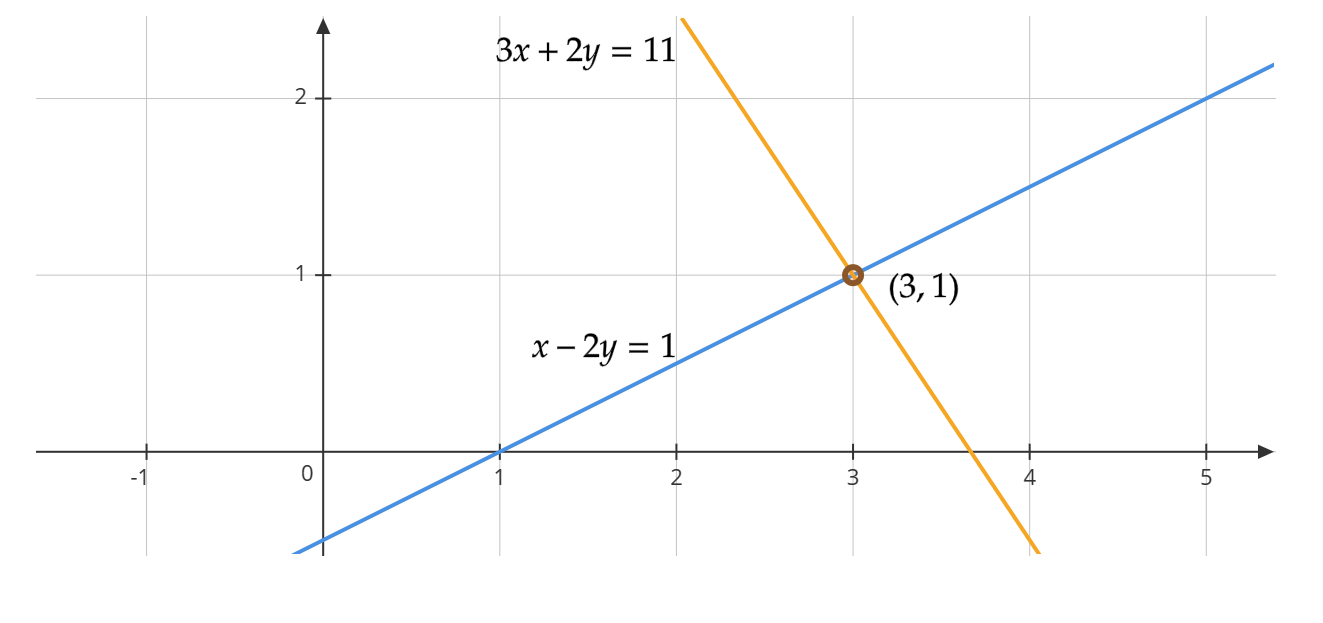
\includegraphics[width=\textwidth]{math-row-picture.png}
        \end{subfigure}
    
       
        \begin{subfigure}[b]{0.8\textwidth}
            \centering
            \caption{Column Picture}
        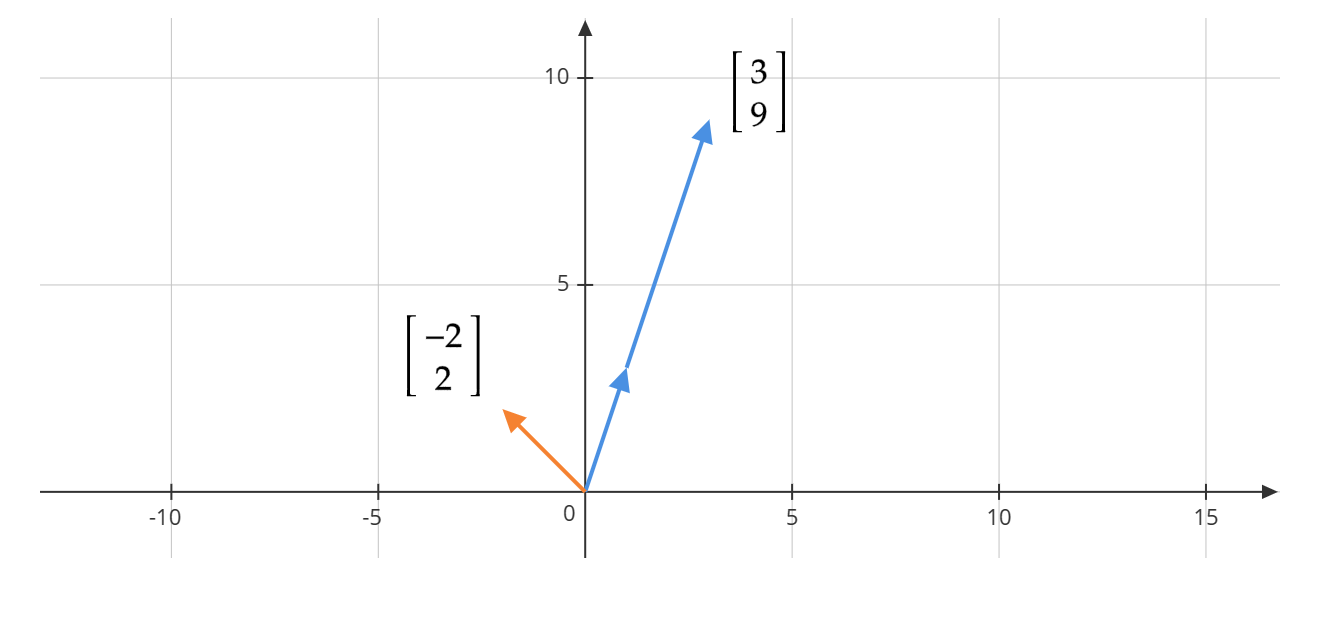
\includegraphics[width=\textwidth]{math-column-picture.png}
        \end{subfigure}
        \end{figure}
    \end{center}
    
\end{example}

\begin{definition}[矩阵-向量乘积函数 $f(x)=A x$]
    给定矩阵 $ A \in \mathbb{R}^{m \times n} $ , 定义函数 $ f: R^{n} \rightarrow R^{m}, f(x)=A x $, 其中 $ A=\left[f\left(e_{1}\right) \ldots f\left(e_{n}\right)\right] $.
\end{definition}

\begin{proof}
    该函数为一个线性函数: $$ A(\alpha x+\beta y)=\alpha(A x)+\beta(A y) $$ 
    
    任意一个线性函数都可以写成矩阵-向量乘积函数的形式

    $$ \begin{aligned} f(x) &=f\left(x_{1} e_{1}+x_{2} e_{2}+\cdots+x_{n} e_{n}\right) \\ &=x_{1} f\left(e_{1}\right)+x_{2} f\left(e_{2}\right)+\cdots+x_{n} f\left(e_{n}\right) \\ &=\left[\begin{array}{lll}f\left(e_{1}\right) & \cdots & f\left(e_{n}\right)\end{array}\right]\left[\begin{array}{c}x_{1} \\ \vdots \\ x_{n}\end{array}\right] \end{aligned} $$

    因此 $ f(x)=A x $, 其中 $ A=\left[f\left(e_{1}\right) \ldots f\left(e_{n}\right)\right] $
\end{proof}

\subsection{Matrix Power}

\begin{definition}[Matrix Power]
    It makes sense to multiply a square matrix $ A $ by itself to form $ A A $. We refer to this matrix as $ A^{2} $. Similarly, if $ k $ is a positive integer, then $ k $ copies of $ A $ multiplied together is denoted $ A^{k} $. If $ k $ and $ l $ are positive integers, and $ A $ is square, then $ A^{k} A^{l}=A^{k+l} $ and $ \left(A^{k}\right)^{l}=A^{k l} $. 
    
    $$ \left(A^{\ell+1}\right)_{i j}=\sum_{k=1}^{n} A_{i k}\left(A^{\ell}\right)_{k j} $$

    By convention we take $ A^{0}=I $, which makes the
    formulas above hold for all nonnegative integer values of $k$ and $l$.
\end{definition}

 \begin{example}[Paths in a directed graph]
        $$ A_{i j}=\left\{\begin{array}{ll}1 & \text { there is a edge from vertex } j \text { to vertex } i \\ 0 & \text { otherwise }\end{array}\right. $$
\end{example}

\begin{example}[Linear dynamical system]
    $$ x_{t+\ell}=A^{\ell} x_{t} $$
\end{example}

\subsection{矩阵乘法的算法复杂度}

\subsubsection{一般矩阵的乘法}

$ C=A B $ with $ A $ of size $ m \times p $ and $ B $ of size $ p \times n $

The product matrix $ C $ has size $ m \times n $, so there are $ m n $ elements to compute. 

The $ i, j $ element of $ C $ is the inner product of row $ i $ of $ A $ with column $ j $ of $ B . $ This is an inner product of vectors of length $ p $ and requires $ 2 p-1 $ flops. Therefore the total is $ m n(2 p-1) $ flops, which we approximate as $ 2 m n p $ flops. $O(mnp)$

\subsubsection{稀疏矩阵的乘法}

Suppose that $ A $ is $ m \times p $ and sparse, and $ B $ is $ p \times n $, but not necessarily sparse. 

The inner product of the $ i $ th row $ a_{i}^{T} $ of $ A $ with the $ j $ th column of $ B $ requires no more than $ 2 \operatorname{nnz}\left(a_{i}^{T}\right) $ flops. 

Summing over $ i=1, \ldots, m $ and $ j=1, \ldots, n $ we get $ 2 \mathbf{n n z}(A) n $ flops. 

If $ B $ is sparse, the total number of flops is no more that $ 2 \mathbf{n n z}(B) m $ flops. 

\begin{remark}
    Note that these formulas agree with the one given above, $ 2 m n p $, when the sparse matrices have all entries nonzero.
\end{remark}

\subsubsection{三重矩阵相乘}

$$ D=A B C $$

with $ A $ of size $ m \times n, B $ of size $ n \times p $, and $ C $ of size $ p \times q $. 

The matrix $ D $ can be computed in two ways, as $ (A B) C $ and as $ A(B C) $. 

In the first method we start with $ A B(2 m n p $ flops) and then form $ D=(A B) C(2 m p q $ flops $ ) $, for a total of $ 2 m p(n+q) $ flops. 

In the second method we compute the product $ B C $ (2npq flops) and then form $ D=A(B C)(2 m n q $ flops), for a total of $ 2 n q(m+p) $ flops.

\begin{remark}
    You might guess that the total number of flops required is the same with the two methods, but it turns out it is not. The first method is less expensive when $ 2 m p(n+q)<2 n q(m+p) $, i.e., when
$$
\frac{1}{n}+\frac{1}{q}<\frac{1}{m}+\frac{1}{p}
$$
\end{remark}

\begin{example}
    As a more specific example, consider the product 
    
    $$ a b^{T} c $$
    
    where $ a, b, c $ are $ n $ vectors. 
    
    If we first evaluate the outer product $ a b^{T} $, the cost is $ n^{2} $ flops, and we need to store $ n^{2} $ values. We then multiply the vector $ c $ by this $ n \times n $ matrix, which costs $ 2 n^{2} $ flops. The total cost is $ 3 n^{2} $ flops.

    If we first evaluate the inner product $b^Tc$, the cost is $2n$ flops, and we only need to store one number (the result). Multiplying the vector a by this number costs $n$ flops, so the total cost is $3n$ flops. For $n$ large, there is a dramatic difference between $3n$ and $3n^2$ flops.

    (The storage requirements are also dramatically different for the two methods of evaluating $ab^Tc$: $1$ number versus $n^2$ numbers.)
\end{example}

\subsection{矩阵向量乘积复杂度}

矩阵 $ A \in \mathbb{R}^{m \times n} $ 和向量 $ x \in \mathbb{R}^{n} $ 的乘积 $ \mathrm{y}=\mathrm{A} x $, 需要 $ (2 \mathrm{n}-1) \mathrm{m} $ flops;

乘积 $ y \in \mathbb{R}^{m} $ , 每个元素需要做向量内积, 需要 $ 2 n-1 $ flops;

当n足够大时, 复杂度近似于2mn;

特殊情况:

\begin{itemize}
    \item $A$为对角矩阵: $ \mathrm{n} $ flops
    \item $A$为下三角矩阵: $ n^{2} $ flops
    \item $A$为稀疏矩阵时:flops $ <<2 m n $
\end{itemize}


\section{Special Matrices and Matrices in Different Applications}

\begin{definition}[Zero Matrix]
    所有元素都为0的矩阵.

    记作$$0, 0_{m \times n} $$
\end{definition}

\begin{definition}[单位矩阵]
    为方形矩阵, 其中对角线元素为1, 其它元素为0.

    记作$I$或者 $ \mathrm{I}_{n} $.
\end{definition}

\begin{corollary}
  $ \mathrm{I}_{n} $ 的每一列是一个单位向量, 例如

$$
\mathrm{I}_{3}=\left[\begin{array}{lll}
1 & 0 & 0 \\
0 & 1 & 0 \\
0 & 0 & 1
\end{array}\right]=\left[\begin{array}{lll}
e_{1} & e_{2} & e_{3}
\end{array}\right]
$$
\end{corollary}

\begin{definition}[Symmetric Matrices]
    $$ A_{i j}=A_{j i}, A^T =A $$
\end{definition}

\begin{definition}[Hermitian Matrices]
    $ A_{i j}=\bar{A}_{j i}, A^H = A $ (共轭复数).
\end{definition}

\begin{definition}[Diagonal Matrices]
    对角线上元素不全为0, 其余元素全为0.
\end{definition}

对角矩阵用于膨胀 (dilation).

\begin{definition}[下三角矩阵]
    方形矩阵且当 $ i<j $ 时 $ A_{i j}=0 $.
\end{definition}

\begin{definition}[上三角矩阵]
    方形矩阵且当 $ i>j $ 时 $ A_{i j}=0 $
\end{definition}

通过Gram-Schmidt正交化算法可以化为上三角或者下三角矩阵。

\subsection{$f(x)=A x$中的$A$}

引入上节$f(x)=A x$(矩阵-向量乘积函数)的概念,

\begin{example}[Permutation Matrices]
    $ f $ 颠倒向量 $ x $ 中的元素的顺序, 一个线性函数 $ f(x)=A x $

    $$ A=\left[\begin{array}{lll}0 & 0 & 1 \\ 0 & 1 & 0 \\ 1 & 0 & 0\end{array}\right] $$是一个置换矩阵.
\end{example}

\begin{proof}
    $$ A x=\left[\begin{array}{lll}0 & 0 & 1 \\ 0 & 1 & 0 \\ 1 & 0 & 0\end{array}\right]\left[\begin{array}{l}x_{1} \\ x_{2} \\ x_{3}\end{array}\right]=\left[\begin{array}{l}x_{3} \\ x_{2} \\ x_{1}\end{array}\right] $$
\end{proof}

\begin{example}
    $ f $ 对向量 $ x $ 中的元素进行升序排序, 非线性;
\end{example}

\begin{example}
    $ f $ 将向量 $ x $ 中的元素替换成相应的绝对值, 非线性;
\end{example}

\begin{example}[反转矩阵]
    $$ A=\left[\begin{array}{ccccc}0 & 0 & \cdots & 0 & 1 \\ 0 & 0 & \cdots & 1 & 0 \\ \vdots & \vdots & \therefore & \vdots & \vdots \\ 0 & 1 & \cdots & 0 & 0 \\ 1 & 0 & \cdots & 0 & 0\end{array}\right] $$
\end{example}

\begin{proof}
    $$ A x=\left[\begin{array}{c}x_{n} \\ x_{n-1} \\ \vdots \\ x_{2} \\ x_{1}\end{array}\right] $$
\end{proof}

\begin{example}[循环移位矩阵]
    $$ A=\left[\begin{array}{ccccc}0 & 0 & \cdots & 0 & 1 \\ 1 & 0 & \cdots & 0 & 0 \\ 0 & 1 & \cdots & 0 & 0 \\ \vdots & \vdots & \ddots & \vdots & \vdots \\ 0 & 0 & \cdots & 1 & 0\end{array}\right] $$
\end{example}

\begin{proof}
    $$ A x=\left[\begin{array}{c}x_{n} \\ x_{1} \\ x_{2} \\ \vdots \\ x_{n-1}\end{array}\right] $$
\end{proof}

\begin{example}[旋转矩阵]
    $$ A=\left[\begin{array}{cc}\cos \theta & -\sin \theta \\ \sin \theta & \cos \theta\end{array}\right] $$

    $ \mathrm{A} x $ 将向量 $ x $ 进行旋转, 角度为 $ \theta $.
\end{example}

\begin{example}[Reflection Matrices]
    Suppose that $y$ is the vector obtained by reflecting $x$ through the line
    that passes through the origin, inclined $\theta$ radians with respect to horizontal. Then

    $$ y=\left[\begin{array}{rr}\cos (2 \theta) & \sin (2 \theta) \\ \sin (2 \theta) & -\cos (2 \theta)\end{array}\right] x $$
\end{example}

\subsection{Selectors}

\begin{definition}[Selector matrices]
    
\end{definition}

\begin{definition}[Downsampling]
    
\end{definition}

\subsection{图论:节点弧关联矩阵}
% todo: image

\begin{definition}[关联矩阵]
   假设有向图$G$有$m$个顶点,  $ n $ 条弧, 则关联矩阵$A$大小为 $ m \times n $,其中 

   $$ A_{i j}=\left\{\begin{array}{ll}1 & \text{如果点} i \text{是弧} j \text{的终点 } \\ -1 & \text {如果点}i \text{是弧}j \text{的起点} \\ 0 & \text { 其它 }\end{array}\right. $$
\end{definition}

\subsection{Convolution}
% todo: image

\begin{definition}[一维卷积]
    向量 $ a \in \mathbb{R}^{n} $ 和向量 $ b \in \mathbb{R}^{m} $ 的\textit{卷积}是一个 $ (\mathrm{n}+\mathrm{m}-1) $ 维向量 $ c \in \mathbb{R}^{m+\mathrm{n}-1} $

    $$ c_{k}=\sum_{i+j=k+1} a_{i} b_{j}, \quad k=1, \ldots n+m-1 $$

    记为 $ c=a * b$
\end{definition}

\begin{example}
    设$n=4,  m=3 $



    \tikzset{every picture/.style={line width=0.75pt}} %set default line width to 0.75pt        

    \begin{tikzpicture}[x=0.75pt,y=0.75pt,yscale=-1,xscale=1]
    %uncomment if require: \path (0,300); %set diagram left start at 0, and has height of 300
    
    %Shape: Rectangle [id:dp6383640467867335] 
    \draw  [fill={rgb, 255:red, 245; green, 166; blue, 35 }  ,fill opacity=1 ] (110,54) -- (160.01,54) -- (160.01,79.16) -- (110,79.16) -- cycle ;
    
    %Shape: Rectangle [id:dp9915913508162717] 
    \draw  [fill={rgb, 255:red, 245; green, 166; blue, 35 }  ,fill opacity=1 ] (260.01,54) -- (310.02,54) -- (310.02,79.16) -- (260.01,79.16) -- cycle ;
    %Shape: Rectangle [id:dp7574544776550791] 
    \draw  [fill={rgb, 255:red, 245; green, 166; blue, 35 }  ,fill opacity=1 ] (210,54) -- (260.01,54) -- (260.01,79.16) -- (210,79.16) -- cycle ;
    %Shape: Rectangle [id:dp15668905720803483] 
    \draw  [fill={rgb, 255:red, 245; green, 166; blue, 35 }  ,fill opacity=1 ] (160,54) -- (210.01,54) -- (210.01,79.16) -- (160,79.16) -- cycle ;
    
    %Shape: Rectangle [id:dp517800094810728] 
    \draw  [fill={rgb, 255:red, 126; green, 211; blue, 33 }  ,fill opacity=1 ] (11,90) -- (61.01,90) -- (61.01,115.16) -- (11,115.16) -- cycle ;
    %Shape: Rectangle [id:dp15583903887589012] 
    \draw  [fill={rgb, 255:red, 126; green, 211; blue, 33 }  ,fill opacity=1 ] (61,90) -- (111.01,90) -- (111.01,115.16) -- (61,115.16) -- cycle ;
    %Shape: Rectangle [id:dp4794201673076599] 
    \draw  [fill={rgb, 255:red, 126; green, 211; blue, 33 }  ,fill opacity=1 ] (111,90) -- (161.01,90) -- (161.01,115.16) -- (111,115.16) -- cycle ;
    
    %Shape: Rectangle [id:dp9652913856506695] 
    \draw  [fill={rgb, 255:red, 245; green, 166; blue, 35 }  ,fill opacity=1 ] (110,130) -- (160.01,130) -- (160.01,155.16) -- (110,155.16) -- cycle ;
    
    %Shape: Rectangle [id:dp6681556567962323] 
    \draw  [fill={rgb, 255:red, 245; green, 166; blue, 35 }  ,fill opacity=1 ] (260.01,130) -- (310.02,130) -- (310.02,155.16) -- (260.01,155.16) -- cycle ;
    %Shape: Rectangle [id:dp0819288495364412] 
    \draw  [fill={rgb, 255:red, 245; green, 166; blue, 35 }  ,fill opacity=1 ] (210,130) -- (260.01,130) -- (260.01,155.16) -- (210,155.16) -- cycle ;
    %Shape: Rectangle [id:dp015621153657017217] 
    \draw  [fill={rgb, 255:red, 245; green, 166; blue, 35 }  ,fill opacity=1 ] (160,130) -- (210.01,130) -- (210.01,155.16) -- (160,155.16) -- cycle ;
    
    %Shape: Rectangle [id:dp9772799588063847] 
    \draw  [fill={rgb, 255:red, 126; green, 211; blue, 33 }  ,fill opacity=1 ] (61,166) -- (111.01,166) -- (111.01,191.16) -- (61,191.16) -- cycle ;
    %Shape: Rectangle [id:dp8281584537494973] 
    \draw  [fill={rgb, 255:red, 126; green, 211; blue, 33 }  ,fill opacity=1 ] (111,166) -- (161.01,166) -- (161.01,191.16) -- (111,191.16) -- cycle ;
    %Shape: Rectangle [id:dp20253755057026024] 
    \draw  [fill={rgb, 255:red, 126; green, 211; blue, 33 }  ,fill opacity=1 ] (161,166) -- (211.01,166) -- (211.01,191.16) -- (161,191.16) -- cycle ;
    
    
    % Text Node
    \draw (126,56.4) node [anchor=north west][inner sep=0.75pt]    {$a_{1}$};
    % Text Node
    \draw (176,56.4) node [anchor=north west][inner sep=0.75pt]    {$a_{2}$};
    % Text Node
    \draw (226,56.4) node [anchor=north west][inner sep=0.75pt]    {$a_{3}$};
    % Text Node
    \draw (276,55.4) node [anchor=north west][inner sep=0.75pt]    {$a_{4}$};
    % Text Node
    \draw (127,92.4) node [anchor=north west][inner sep=0.75pt]    {$b_{1}$};
    % Text Node
    \draw (77,92.4) node [anchor=north west][inner sep=0.75pt]    {$b_{2}$};
    % Text Node
    \draw (27,92.4) node [anchor=north west][inner sep=0.75pt]    {$b_{3}$};
    % Text Node
    \draw (77,168.4) node [anchor=north west][inner sep=0.75pt]    {$b_{3}$};
    % Text Node
    \draw (127,168.4) node [anchor=north west][inner sep=0.75pt]    {$b_{2}$};
    % Text Node
    \draw (177,168.4) node [anchor=north west][inner sep=0.75pt]    {$b_{1}$};
    % Text Node
    \draw (276,131.4) node [anchor=north west][inner sep=0.75pt]    {$a_{4}$};
    % Text Node
    \draw (226,132.4) node [anchor=north west][inner sep=0.75pt]    {$a_{3}$};
    % Text Node
    \draw (176,132.4) node [anchor=north west][inner sep=0.75pt]    {$a_{2}$};
    % Text Node
    \draw (126,132.4) node [anchor=north west][inner sep=0.75pt]    {$a_{1}$};
    % Text Node
    \draw (346,78.4) node [anchor=north west][inner sep=0.75pt]  [color={rgb, 255:red, 236; green, 92; blue, 109 }  ,opacity=1 ]  {$c_{1} \ =\ a_{1} b_{1}$};
    % Text Node
    \draw (341,155.4) node [anchor=north west][inner sep=0.75pt]  [color={rgb, 255:red, 236; green, 92; blue, 109 }  ,opacity=1 ]  {$c_{2} \ =\ a_{1} b_{2} +a_{2} b_{1}$};
    
    
    \end{tikzpicture}
    
$$\begin{aligned}
    c_{1}&=a_{1} b_{1}\\
    c_{2}&=a_{1} b_{2}+a_{2} b_{1}\\
    c_{3}&=a_{1} b_{3}+a_{2} b_{2}+a_{3} b_{1}\\
    c_{4}&=a_{2} b_{3}+a_{3} b_{2}+a_{4} b_{1}\\
    c_{5}&=a_{3} b_{3}+a_{4} b_{2}\\
    c_{6}&=a_{4} b_{3}\\
\end{aligned} $$


\end{example}

\begin{corollary}
    假设向量$a$和$b$分别是以下多项式的系数
    $$ p(x)=a_{1}+a_{2} x+\cdots+a_{n} x^{n-1}, q(x)=b_{1}+b_{2} x+\cdots+b_{m} x^{m-1} $$

    则 $ \mathrm{c}=\mathrm{a}^{*} \mathrm{~b} $ 是多项式 $ p(x) q(x) $ 的系数.

    $$ p(x) q(x)=c_{1}+c_{2} x+\cdots+c_{m+n-1} x^{m+n-2} $$
\end{corollary}

\begin{corollary}[卷积性质]
    有如下性质:
    \begin{itemize}
        \item 对称性: $ a * b=b * a $
        \item 结合律: $ (a * b) * c=a *(b * c) $
        \item 如果 $ a * b=0 $, 则 $ a=0 $, 或者 $ b=0 $
    \end{itemize}
\end{corollary}

\begin{corollary}
    如果固定 $ a $或$b$,则 $ c=a * b $ 是一个线性函数
\end{corollary}

\begin{example}[Toeplitz Matrix]
    4维向量a和3维向量 $ b $ ,  则 $ c=a * b $

$$
\left[\begin{array}{l}
c_{1} \\
c_{2} \\
c_{3} \\
c_{4} \\
c_{5} \\
c_{6}
\end{array}\right]=\left[\begin{array}{lll}
a_{1} & 0 & 0 \\
a_{2} & a_{1} & 0 \\
a_{3} & a_{2} & a_{1} \\
a_{4} & a_{3} & a_{2} \\
0 & a_{4} & a_{3} \\
0 & 0 & a_{4}
\end{array}\right]\left[\begin{array}{l}
b_{1} \\
b_{2} \\
b_{3}
\end{array}\right]=\left[\begin{array}{cccc}
b_{1} & 0 & 0 & 0 \\
b_{2} & b_{1} & 0 & 0 \\
b_{3} & b_{2} & b_{1} & 0 \\
0 & b_{3} & b_{2} & b_{1} \\
0 & 0 & b_{3} & b_{2} \\
0 & 0 & 0 & b_{3}
\end{array}\right]\left[\begin{array}{l}
a_{1} \\
a_{2} \\
a_{3} \\
a_{4}
\end{array}\right]
$$
\end{example}

\subsection{多项式}

\begin{definition}[多项式]
    \textit{多项式} $ p(t) $, \textit{度}为 $ n-1 $, \textit{系数}为 $ x_{1}, x_{2}, \ldots, x_{n} $

    $$
p(t)=x_{1}+x_{2} t+x_{3} t^{2}+\cdots+x_{n} t^{n-1}
$$
\end{definition}

\begin{definition}[Vandermonde Matrices]
    $ \mathrm{p}(\mathrm{t}) $ 在m个点中 $ t_{1}, t_{2}, \ldots, t_{m} $ 的值为
    $$
    \left[\begin{array}{c}
    p\left(t_{1}\right) \\
    p\left(t_{2}\right) \\
    \vdots \\
    p\left(t_{m}\right)
    \end{array}\right]=\left[\begin{array}{cccc}
    1 & t_{1} & \cdots & t_{1}^{n-1} \\
    1 & t_{2} & \cdots & t_{2}{ }^{n-1} \\
    \vdots & \vdots & \ddots & \vdots \\
    1 & t_{m} & \cdots & t_{m}{ }^{n-1}
    \end{array}\right]\left[\begin{array}{c}
    x_{1} \\
    x_{2} \\
    \vdots \\
    x_{n}
    \end{array}\right]=A x
    $$

    矩阵$A$被称为\textit{Vandermonde矩阵}.
\end{definition}

\subsection{Fourier Transform}

\begin{definition}[Discrete Fourier Transform (DFT)]
    DFT将 $ n $ 维复向量 $ x $ 映射为 $ {n} $ 维复向量 $ y\left(\mathbb{C}^{n} \rightarrow \mathbb{C}^{n}\right) $

    $$ y_{k}=\sum_{\ell=1}^{n} x_{\ell} e^{-i \frac{2 \pi}{n}(k-1)(\ell-1)}, k=1, \cdots, n $$

    $$ \left[\begin{array}{c}y_{1} \\ y_{2} \\ y_{3} \\ \vdots \\ y_{n}\end{array}\right]=\left[\begin{array}{ccccc}1 & 1 & 1 & \cdots & 1 \\ 1 & \omega^{-1} & \omega^{-2} & \cdots & \omega^{-(n-1)} \\ 1 & \omega^{-2} & \omega^{-4} & \cdots & \omega^{-2(n-1)} \\ \vdots & \vdots & \vdots & \cdots & \vdots \\ 1 & \omega^{-(n-1)} & \omega^{-2(n-1)} & \cdots & \omega^{-(n-1)(n-1)}\end{array}\right]\left[\begin{array}{c}x_{1} \\ x_{2} \\ x_{3} \\ \vdots \\ x_{n}\end{array}\right] $$

   其中 $ \omega=e^{2 \pi i / n} $.
\end{definition}

DFT矩阵W的第 $ k $ 行第 $ l $ 列的元素为 $ W_{k l}=\omega^{-(k-1)(l-1)} $.

\begin{definition}[Discrete Inverse Fourier Transform]
    $$ x_{\ell}=\frac{1}{n} \sum_{k=1}^{n} y_{k} e^{i \frac{2 \pi}{n}(k-1)(\ell-1)}, \ell=1, \cdots, n $$
\end{definition}

\subsection{Semi-Definite Matrices}

\begin{definition}[半正定矩阵]
    对称矩阵 $ A \in \mathbb{R}^{n \times n} $ 称为\textit{半正定矩阵}, 满足以下条件

$$
x^{T} A x \geq 0 \quad \forall x \in \mathbb{R}^{n}
$$
\end{definition}

\begin{definition}[正定矩阵]
    对称矩阵 $ A \in \mathbb{R}^{n \times n} $ 称为正定矩阵, 满足以下条件
$$
x^{T} A x>0 \quad \forall x \neq 0
$$
\end{definition}

\begin{definition}[二次型]
    如果对称矩阵 $ A \in \mathbb{R}^{n \times n} $, 则 $ x^{T} A x $ 是二次型
\end{definition}

\begin{proof}
    $$ x^{T} A x=\sum_{i=1}^{n} \sum_{j=1}^{n} x_{i} A_{i j} x_{j}=\sum_{i=1}^{n} A_{i i} x_{i}^{2}+2 \sum_{i>j} A_{i j} x_{i} x_{j} $$
\end{proof}

\begin{example}
    $$ A=\left[\begin{array}{ll}9 & 6 \\ 6 & a\end{array}\right] $$

    $$ x^{T} A x=9 x_{1}^{2}+12 x_{1} x_{2}+a x_{2}^{2}=\left(3 x_{1}+2 x_{2}\right)^{2}+(a-4) x_{2}^{2} $$

    如果 $ a>4 $, 矩阵 $ A $ 为正定矩阵:
$$
x^{T} A x>0 \quad \forall x \neq 0
$$

如果 $ a=4 $, 矩阵 $ A $ 为半正定矩阵, 但不是正定矩阵:
$$
x^{T} A x \geq 0 \quad \forall x, \quad x^{T} A x=0 \quad \exists x=\left[\begin{array}{l}
2 \\
-3
\end{array}\right]
$$

如果 $ a<4 $, 矩阵 $ A $ 不是半正定矩阵:
$$
x^{T} A x<0 \quad \exists x=\left[\begin{array}{l}
2 \\
-3
\end{array}\right]
$$
\end{example}

\begin{corollary}
    正定矩阵 $ A $ 都是非奇异的.
\end{corollary}

\begin{proof}
    $$ A x=0 \quad \Rightarrow \quad x^{T} A x=0 \quad \Rightarrow \quad x=0 $$

    最后一步由正定性得到的.($
    x^{T} A x>0 \quad \forall x \neq 0
    $)

\end{proof}

\begin{theorem}[正定矩阵对角元素性质]
    正定矩阵 $ A $ 有正的对角元素.

    $$
A_{i i}=e_{i}^{T} A e_{i}>0
$$
\end{theorem}

\begin{theorem}[半正定矩阵对角元素性质]
    每个半正定矩阵 $ A $ 都有非负的对角元素.
$$
A_{i i}=e_{i}^{T} A e_{i} \geq 0
$$
\end{theorem}

\section{Gram 矩阵}

\begin{definition}[实矩阵$A$的Gram矩阵]
    \label{Def:Gram}

    $$ G=A^{T} A=\left[\begin{array}{c}a_{1}^{T} \\ a_{2}^{T} \\ \vdots \\ a_{n}^{T}\end{array}\right]\left[a_{1}, a_{2}, \cdots, a_{n}\right]=\left[\begin{array}{cccc}a_{1}^{T} a_{1} & a_{1}^{T} a_{2} & \cdots & a_{1}^{T} a_{n} \\ a_{2}^{T} a_{1} & a_{2}^{T} a_{2} & \cdots & a_{2}^{T} a_{n} \\ \vdots & \vdots & \ddots & \vdots \\ a_{n}^{T} a_{1} & a_{n}^{T} a_{2} & \cdots & a_{n}^{T} a_{n}\end{array}\right] $$
\end{definition}

\begin{definition}[复矩阵的$A$的Gram 矩阵]
    $$ G=A^{H} A=\left[\begin{array}{cccc}a_{1}^{H} a_{1} & a_{1}^{H} a_{2} & \cdots & a_{1}^{H} a_{n} \\ a_{2}^{H} a_{1} & a_{2}^{H} a_{2} & \cdots & a_{2}^{H} a_{n} \\ \vdots & \vdots & \ddots & \vdots \\ a_{n}^{H} a_{1} & a_{n}^{H} a_{2} & \cdots & a_{n}^{H} a_{n}\end{array}\right] $$
\end{definition}

\begin{theorem}
    每个Gram矩阵都是半正定的.
\end{theorem}

\begin{proof}
    $$ x^{T} A x=x^{T} B^{T} B x=\|B x\|_{2}^{2} \geq 0 , \forall x $$
\end{proof}

\begin{theorem}
    如果Gram矩阵是正定的, 则要满足
    $$ x^{T} A x=x^{T} B^{T} B x=\|B x\|_{2}^{2}>0 ( \forall x \neq 0) $$
\end{theorem}

\begin{corollary}
    如果Gram矩阵是正定的, 则$B$的列向量是线性无关的.
\end{corollary}

\begin{proof}
    $$\|B x\|_{2}^{2}>0 ( \forall x \neq 0)$$

所以 $\forall x \neq 0, Bx \neq 0  $.

    注意和线性无关 \ref{Def:LinearIndependence} 的定义进行参照.
\end{proof}

\chapter{Matrices Norms}

\section{矩阵范数}

\begin{definition}[Matrix Norm]
    向量空间中存在一个函数 $ \|\cdot\|: \mathbb{R}^{m \times n} \rightarrow \mathbb{R} $

    且满足以下条件:

    \begin{itemize}
        \item 齐次性: $ \|\alpha A\|=|\alpha|\|A\|, \alpha \in \mathbb{R} $ 且 $ A \in \mathbb{R}^{m \times n} $;
        \item 三角不等式: $ \|A+B\| \leq\|A\|+\|B\|, A, B \in \mathbb{R}^{m \times n} $;
        \item 非负性: $ \|A\| \geq 0, A \in \mathbb{R}^{m \times n} $ 且 $ \|A\|=0 \Leftrightarrow A=0 $;
    \end{itemize}

则称 $ \|\cdot\| $ 为矩阵范数. 
\end{definition}

向量空间 $ \mathbb{R}^{m \times n} $ 矩阵范数:

\begin{example}[F-范数(Frobenius norm)]
    $$ \|A\|_{F}=\left(\sum_{i=1}^{n} \sum_{j=1}^{n} a_{i j}^{2}\right)^{\frac{1}{2}} $$
\end{example}

\begin{proof}
    $$ \|A\|_{F} \geq 0 $$

    $$ \|\alpha A\|_{F}=|\alpha|\|A\|_{F}, \alpha \in \mathbb{R} $$

    $$ \begin{aligned}\|A+B\|_{F}=&\left(\sum_{i=1}^{n} \sum_{j=1}^{n}\left(a_{i j}+b_{i j}\right)^{2}\right)^{\frac{1}{2}} \leq\left(\sum_{i=1}^{n} \sum_{j=1}^{n}\left(a_{i j}\right)^{2}\right)^{\frac{1}{2}}+\left(\sum_{i=1}^{n} \sum_{j=1}^{n}\left(b_{i j}\right)^{2}\right)^{\frac{1}{2}} \\ &=\|A\|_{F}+\|B\|_{F} \end{aligned} $$
\end{proof}

\begin{definition}[从属于给定向量范数 $ \|x\|_{v} $ 的矩阵范数]
    设 $ x \in \mathbb{R}^{n}, A \in \mathbb{R}^{m \times n},\|\cdot\|_{v} $ 为一种向量范数. 则 $ \frac{\|A x\|_{v}}{\|x\|_{v}} $ 对所有 $ x \neq 0 $ 有最大值, 令

    $$ \|A\|_{v}=\max _{x \neq 0}\left\{\frac{\|A x\|_{v}}{\|x\|_{v}}\right\}=\max _{x \neq 0}\left\{\left\|A \frac{x}{\|x\|_{v}}\right\|_{v}\right\}=\max _{\|y\|_{v}=1}\left\{\|A y\|_{v}\right\} $$

    即$$ \|A\|_{v}=\max _{x \neq 0}\left\{\frac{\|A x\|_{v}}{\|x\|_{v}}\right\} $$

    $ \|A\|_{v} $ 称为从属于给定向量范数 $ \|x\|_{v} $ 的矩阵范数, 简称为\term{从属范数}或\term{算子范数}.
\end{definition}

\begin{proof}
    可以验证 $ \|A\|_{v} $ 满足矩阵范数定义. 

    $$ \|A\|_{v} \geq 0 $$

    $$ \|\alpha A\|_{v}=|\alpha|\|A\|_{v}, \alpha \in \mathbb{R} $$

    $$\begin{aligned}
        \|A+B\|_{v} &=\max _{\|y\|_{v}=1}\|(A+B) y\|_{v} \\
        &\leq \max _{\|y\|_{v}=1}\left\{\|A y\|_{v}+\|B y\|_{v}\right\} \\
        & \leq \max _{\|y\|_{v}=1}\|A y\|_{v}+\max _{\|y\|_{v}=1}\|B y\|_{v} \\
        & =\|A\|_{v}+\|B\|_{v}
    \end{aligned}$$

\end{proof}

\begin{remark}
    在本书中若未明确说明, $\|A \|$表示的是算子范数.
\end{remark}

由定义 $ \|A\|_{v}=\max _{x \neq 0}\left\{\frac{\|A x\|_{v}}{\|x\|_{v}}\right\} $ 可得

\begin{definition}[向量范数和算子范数相容]
    $$ \frac{\|A x\|_{v}}{\|x\|_{v}} \leq\|A\|_{v} \Rightarrow\|A x\|_{v} \leq\|A\|_{v}\|x\|_{v} $$

    称向量范数和算子范数\textit{相容}. 
\end{definition}

\begin{theorem}[算子范数服从乘法范数相容性]
   对于 $ A \in \mathbb{R}^{m \times n}, B \in \mathbb{R}^{n \times p} $

    $$\begin{aligned}
        \|A B\|_{v} &=\max _{x \neq 0}\left\{\frac{\|A B x\|_{v}}{\|x\|_{v}}\right\} \\
        & \leq \max _{x \neq 0}\left\{\frac{\|A\|_{v}\|B x\|_{v}}{\|x\|_{v}}\right\} \\
        & \leq\|A\|_{v} \max _{x \neq 0}\left\{\frac{\|B\|_{v}\|x\|_{v}}{\|x\|_{v}}\right\} \\
        & =\|A\|_{v}\|B\|_{v}
    \end{aligned}$$
    算子范数服从\textit{乘法范数相容性}.
\end{theorem}

根据向量的常用范数可以导出矩阵 $ A \in \mathbb{R}^{m \times n} $ 的算子范数

\begin{definition}[$A$的列范数]
    $$ \|A\|_{1}=\max _{x \neq 0}\left(\frac{\|A x\|_{1}}{\|x\|_{1}}\right)=\max _{1 \leq j \leq n} \sum_{i=1}^{m}\left|a_{i j}\right| $$
\end{definition}

\begin{definition}[$A$的行范数]
    $$ \|A\|_{\infty}=\max _{x \neq 0}\left( \frac{\|A x\|_{\infty}}{\|x\|_{\infty}}    \right)=\max _{1 \leq i \leq m} \sum_{j=1}^{n}\left|a_{i j}\right| $$
\end{definition}

\begin{definition}[$A$的2−范数]
    $$ \|A\|_{2}=\max _{x \neq 0}\left( \frac{\|A x\|_{2}}{\|x\|_{2}}  \right)=\sqrt{\lambda_{\max }\left(A^{T} A\right)} $$
\end{definition}

\begin{example}
    求矩阵$A$的各种常用范数
$$
A=\left(\begin{array}{ccc}
1 & 2 & 0 \\
-1 & 2 & -1 \\
0 & 1 & 1
\end{array}\right)
$$

$$ \|A\|_{1}=\max _{1 \leq j \leq n} \sum_{i=1}^{n}\left|a_{i j}\right|=\max _{1 \leq j \leq n}\{2,5,2\}=5 $$

$$ \|A\|_{\infty}=\max _{1 \leq i \leq n} \sum_{j=1}^{n}\left|a_{i j}\right|=\max _{1 \leq i \leq n}\{3,4,2\}=4 $$

由于 $ \|A\|_{2}=\sqrt{\lambda_{\max }\left(A^{T} A\right)} $
, 因此先求 $ A^{T} A $ 的特征值

$$ A^{T} A=\left(\begin{array}{ccc}1 & -1 & 0 \\ 2 & 2 & 1 \\ 0 & -1 & 1\end{array}\right) \cdot\left(\begin{array}{ccc}1 & 2 & 0 \\ -1 & 2 & -1 \\ 0 & 1 & 1\end{array}\right)=\left(\begin{array}{ccc}2 & 0 & 1 \\ 0 & 9 & -1 \\ 1 & -1 & 2\end{array}\right) $$

特征方程为

$$ \operatorname{det}\left(\lambda I-A^{T} A\right)=\left|\begin{array}{ccc}\lambda-2 & 0 & -1 \\ 0 & \lambda-9 & 1 \\ -1 & 1 & \lambda-2\end{array}\right|=0 $$

可得 $ A^{T} A $ 的特征值

$$ \lambda_{1}=9.1428, \lambda_{2}=2.9211, \lambda_{3}=0.9361 $$

\end{example}

\begin{remark}
    对于$\|A\|_{2}$需要计算$\lambda_{\max }\left(A^{T} A\right)$, 直接根据特征方程计算特征值的算法复杂度太高.
\end{remark}

\chapter{适定问题}

\section{The Definition of Well-posed Problem}

In 1923, the French mathematician Hadamard introduced the notion of well-posed (适定)  problem:

\begin{itemize}
    \item A solution for the problem exists;
    \item The solution is unique;
    \item Perturbations in the data should cause small perturbations in the solution.
\end{itemize}

One of these conditions is not satisfied, the problem is said to be ill-posed (病态) and demands a special consideration.

\begin{example}
    假设 $ A $ 是非奇异矩阵 $$ A x=b $$

    如果将 $ b $ 为 $ b+\Delta b $, 方程新的解 $ x+\Delta x $, 则有:
$$
A(x+\Delta x)=b+\Delta b
$$

即
$$
\Delta x=A^{-1} \Delta b
$$

如果小的变化 $ \Delta b $ 导致小变化 $ \Delta x $, 则称解是\textit{稳定}的. 如果小的变化 $ \Delta b $ 导致大变化 $ \Delta x $, 则称解\textit{不稳定}的. 

设$$ A=\frac{1}{2}\left[\begin{array}{cc}1 & 1 \\ 1+10^{-10} & 1-10^{-10}\end{array}\right], \quad A^{-1}=\left[\begin{array}{cc}1-10^{10} & 10^{10} \\ 1+10^{10} & -10^{10}\end{array}\right] $$

若$ b=(1,1) $, 方程 $ A x $ 的解 $ x=(1,1) $ . 
如果将b改为 $ b+\Delta b $ , 那么 $ x $ 的变化量为

$$ \Delta x=A^{-1} \Delta b=\left[\begin{array}{l}\Delta b_{1}-10^{10}\left(\Delta b_{1}-\Delta b_{2}\right) \\ \Delta b_{1}+10^{10}\left(\Delta b_{1}-\Delta b_{2}\right)\end{array}\right] $$

很小变化 $ \Delta b $ 会导致非常大变化 $ \Delta x $! 由矩阵$A$定义的问题, 称为\textit{适定问题}或\textit{病态问题}. 

\end{example}

\section{绝对误差的界限}

假设 $ A $ 是非奇异的, 并给出定义:

\begin{notation}
    $$ x=A^{-1} b$$ 
    
    $$ \Delta x=A^{-1} \Delta b $$
\end{notation}

$ \|\Delta x\| $ 的上界为:
$$
\|\Delta x\|_{2} \leq\left\|A^{-1}\right\|_{2}\|\Delta b\|_{2}
$$

矩阵范数 $ \left\|A^{-1}\right\|_{2} $ 小时, 当 $ \|\Delta b\|_{2} $ 变化很小, $ \|\Delta x\|_{2} $ 也很小; $ \left\|A^{-1}\right\|_{2} $ 大时,  $ \|\Delta x\|_{2} $ 可能很大,  即使 $ \|\Delta b\|_{2} $ 很小. 

\section{相对误差的界限}

假设 $ b \neq 0 $; 因此 $ x \neq 0$

$\|\Delta x\|_{2} /\|x\|_{2} $ 的上界为:

$$ 
\begin{aligned}
    &\|\Delta x\|_{2}=\left\|A^{-1} \Delta b\right\|_{2} \leq\left\|A^{-1}\right\|_{2}\|\Delta b\|_{2}(向量范数和算子范数相容)\\
    \Rightarrow& \frac{\|\Delta x\|_{2}}{\|x\|_{2}} \leq \frac{\left\|A^{-1}\right\|_{2}\|\Delta b\|_{2}}{\|x\|_{2}}=\frac{\|A\|_{2}\left\|A^{-1}\right\|_{2}\|\Delta b\|_{2}}{\|x\|_{2}\|A\|_{2}} \leq \frac{\|A\|_{2}\left\|A^{-1}\right\|_{2}\|\Delta b\|_{2}}{\|b\|_{2}}
\end{aligned}
$$

由 $ \|b\|_{2}=\|A x\|_{2} \leq\|A\|_{2}\|x\|_{2} $, 可得

$$ \frac{\|\Delta x\|_{2}}{\|x\|_{2}} \leq\|A\|_{2}\left\|A^{-1}\right\|_{2} \frac{\|\Delta b\|_{2}}{\|b\|_{2}} $$

$ \|A\|_{2}\left\|A^{-1}\right\|_{2} $ 小,当 $ \frac{\|\Delta b\|_{2}}{\|b\|_{2}}  $ 相对变化很小时, $ \frac{\|\Delta x\|_{2}}{\|x\|_{2}}  $ 也 变化很小;

$ \|A\|_{2}\left\|A^{-1}\right\|_{2} $ 大, $ \frac{\|\Delta x\|_{2}}{\|x\|_{2}}  $ 可远远大于 $ \frac{\|\Delta b\|_{2}}{\|b\|_{2}}  $.


\begin{definition}[非奇异矩阵 $ A $ 的条件数(condition number)]
    $$ \kappa(A)=\|A\|_{2}\left\|A^{-1}\right\|_{2} $$
\end{definition}

\begin{corollary}[非奇异矩阵 $ A $ 的条件数(condition number)性质]
    有如下性质:

    \begin{itemize}
        \item 对于所有 $ A $, 有 $ \kappa(A) \geq 1 $;
        \item 如果 $ \kappa(A) $ 比较小 (接近1),  $ x $ 的相对误差接近 $ b $ 的相对误差;
        \item 如果 $ \kappa(A) $ 比较大(超过100),  $ x $ 的相对误差比 $ b $ 的相对误差大得多. 
    \end{itemize}
\end{corollary}



\chapter{Inverse of Matrices}

\section{Left Inverse, Right Inverse, Inverse}

\begin{definition}[$A$的左逆]
    当一个矩阵X满足 $$ X A=I $$ 
    
    X被称为 $ A $ 的\textit{左逆}; 当左逆存在时,则称A是\textit{可左逆}的;
\end{definition}

    如果左逆矩阵存在, 则左逆矩阵有\textbf{无穷多}个.

\begin{example}
    $$ A=\left[\begin{array}{cc}-3 & -4 \\ 4 & 6 \\ 1 & 1\end{array}\right] $$

    矩阵$A$是可左逆的,其左逆矩阵有两个

    $$ B=\frac{1}{9}\left[\begin{array}{ccc}-11 & -10 & 16 \\ 7 & 8 & -11\end{array}\right] \quad C=\frac{1}{2}\left[\begin{array}{ccc}0 & -1 & 6 \\ 0 & 1 & -4\end{array}\right] $$
\end{example}

\begin{definition}[$A$的右逆]
    当左逆存在时,则称A是可左逆的;
\end{definition}

    如果右逆矩阵存在, 则右逆矩阵有\textbf{无穷多}个.


\begin{example}
    $$ B=\left[\begin{array}{lll}1 & 0 & 1 \\ 0 & 1 & 1\end{array}\right] $$

    矩阵$B$可右逆,以下矩阵都是$B$的右逆

    $$ D=\frac{1}{2}\left[\begin{array}{cc}1 & -1 \\ -1 & 1 \\ 1 & 1\end{array}\right], E=\left[\begin{array}{ll}1 & 0 \\ 0 & 1 \\ 0 & 0\end{array}\right], G=\left[\begin{array}{cc}1 & -1 \\ 0 & 0 \\ 0 & 1\end{array}\right] $$
\end{example}

一个大小为 $ m \times n $ 的矩阵, 其左逆或右逆的维度为 $ n \times m $.

\begin{theorem}
    A的左逆为 $ X $ 当且仅当 $ X^{T} $ 是 $ A^{T} $ 的右逆.
\end{theorem}

\begin{proof}
    $$
A^{T} X^{T}=(X A)^{T}=I
$$
\end{proof}

\begin{theorem}
    A的右逆为 $ X $ 当且仅当 $ X^{T} $ 是 $ A^{T} $ 的左逆.
\end{theorem}

\begin{proof}
    $$
X^{T} A^{T}=(A X)^{\mathrm{T}}=I
$$
\end{proof}

\begin{theorem}
    如果矩阵A存在左逆和右逆,则左逆和右逆一定相等
\end{theorem}

\begin{proof}
    $$
    \begin{aligned}
    &X A=I, A Y=I  \\
    \Rightarrow&  X=X I=X(A Y)=(X A) Y=Y \\
    \Rightarrow& X=Y
    \end{aligned}
$$
\end{proof}

\begin{definition}
    如果矩阵A存在左逆和右逆, 此时X称为矩阵的\textit{逆},记作 $ A^{-1} $ 当矩阵的逆存在时,则称矩阵A\textit{可逆}.
\end{definition}

\section{Linear Equation Systems}

\begin{definition}
    有$n$个变量的$m$个方程为

    $$ \left\{\begin{array}{c}A_{11} x_{1}+A_{12} x_{2}+\cdots+A_{1 n} x_{n}=b_{1} \\ A_{21} x_{1}+A_{22} x_{2}+\cdots+A_{2 n} x_{n}=b_{2} \\ \vdots \\ A_{m 1} x_{1}+A_{m 2} x_{2}+\cdots+A_{m n} x_{n}=b_{m}\end{array}\right. $$

    写成矩阵形式为: $ \mathrm{A} x=\mathrm{b} $ . 其中$A$为系数矩阵, $ x $ 为$n$维列向量. 
\end{definition}

该方程组可能\textbf{无解},\textbf{有唯一解}和\textbf{无穷解}.

\subsection{线性方程组求解}

\begin{theorem}
    如果矩阵$A$可左逆,假设 $ X $ 是矩阵$A$的左逆,则\textbf{至多}一个解, 如有解则 $ x=X b $ . 
\end{theorem}

\begin{proof}
    $$
A x=b \Rightarrow  x=X A x=X b
$$

    列满秩时(下面证明), 列向量线性无关, 所以其零空间中只有零解,方程 $ {Ax}={b} $ 可能有一个唯一解 ($b$在$A$的列空间中, 此特解就是全部解, 因为通常的特解可以通过零空间中的向量扩展出一组解集,而此时零空间只有$0$向量), 也可能无解 ($b$不在$A$的列空间中). 
\end{proof}

\begin{theorem}
    如果矩阵$A$可右逆,假设 $ Y $ 是矩阵$A$的右逆,则\textbf{至少}一个解, 即 $ x=\mathrm{Y} b $ . 
\end{theorem}

\begin{proof}
    设$x=Y b$ 

    $$
x=Y b  \Rightarrow  A x=A Y b=b
$$


右逆就是研究 $m \times n $ 矩阵$A$行满秩的情况, 此时 $ \mathrm{n}>\mathrm{m}=\operatorname{rank}(\mathrm{A}) $ . 对称的, 其左零空间中仅有零向量,即没有行向量的线性组合能够得到零向量. ($N(A ^T ) = \{0\}$)
\end{proof}

\begin{theorem}
    如果矩阵$A$可逆的,假设 $ X $ 是矩阵$A$的逆,则
$$
A x=b  \Rightarrow  x=A^{-1} b
$$
唯一解. 
\end{theorem}

\subsection{Fundamental Theorem of Linear Algebra}


\tikzset{every picture/.style={line width=0.75pt}} %set default line width to 0.75pt        
% \resizebox{\textwidth}{!}{%
\begin{tikzpicture}[x=0.75pt,y=0.75pt,yscale=-0.9,xscale=0.9]

%\begin{adjustbox}{width=\textwidth}
%\begin{tikzpicture}   
%uncomment if require: \path (0,300); %set diagram left start at 0, and has height of 300

%Shape: Rectangle [id:dp8564537788335302] 
\draw  [dash pattern={on 0.84pt off 2.51pt}] (221.63,153.4) -- (253.96,185.17) -- (225.93,213.7) -- (193.59,181.93) -- cycle ;
%Shape: Rectangle [id:dp7748103688398633] 
\draw   (159.81,65.14) -- (236.34,135.27) -- (193.59,181.93) -- (117.06,111.79) -- cycle ;
%Shape: Rectangle [id:dp3534850306924755] 
\draw   (193.59,181.93) -- (260.03,242.81) -- (218.64,287.99) -- (152.2,227.1) -- cycle ;

%Shape: Rectangle [id:dp11468847928918202] 
\draw   (477.03,52.53) -- (398.27,134.34) -- (440.51,175) -- (519.26,93.19) -- cycle ;
%Shape: Rectangle [id:dp8320016424104848] 
\draw   (440.51,175) -- (372.14,246.02) -- (413.05,285.39) -- (481.41,214.38) -- cycle ;

%Straight Lines [id:da413550032058265] 
\draw [color={rgb, 255:red, 139; green, 87; blue, 42 }  ,draw opacity=1 ][line width=2.25]    (193.59,181.93) -- (217.74,155.81) ;
\draw [shift={(221.14,152.14)}, rotate = 492.75] [fill={rgb, 255:red, 139; green, 87; blue, 42 }  ,fill opacity=1 ][line width=0.08]  [draw opacity=0] (8.57,-4.12) -- (0,0) -- (8.57,4.12) -- cycle    ;
%Straight Lines [id:da05215716031511208] 
\draw [color={rgb, 255:red, 245; green, 166; blue, 35 }  ,draw opacity=1 ][line width=2.25]    (193.59,181.93) -- (222.99,209.56) ;
\draw [shift={(226.64,212.99)}, rotate = 223.23] [fill={rgb, 255:red, 245; green, 166; blue, 35 }  ,fill opacity=1 ][line width=0.08]  [draw opacity=0] (8.57,-4.12) -- (0,0) -- (8.57,4.12) -- cycle    ;
%Straight Lines [id:da20598638562684246] 
\draw [color={rgb, 255:red, 65; green, 117; blue, 5 }  ,draw opacity=1 ][line width=2.25]    (193.59,181.93) -- (248.97,184.9) ;
\draw [shift={(253.96,185.17)}, rotate = 183.08] [fill={rgb, 255:red, 65; green, 117; blue, 5 }  ,fill opacity=1 ][line width=0.08]  [draw opacity=0] (8.57,-4.12) -- (0,0) -- (8.57,4.12) -- cycle    ;
%Straight Lines [id:da9574000480451021] 
\draw  [dash pattern={on 4.5pt off 4.5pt}]  (221.14,152.14) -- (435.64,119.99) ;
\draw [shift={(328.39,136.06)}, rotate = 531.48] [fill={rgb, 255:red, 0; green, 0; blue, 0 }  ][line width=0.08]  [draw opacity=0] (8.93,-4.29) -- (0,0) -- (8.93,4.29) -- cycle    ;
%Straight Lines [id:da8574440156945131] 
\draw  [dash pattern={on 4.5pt off 4.5pt}]  (253.96,185.17) -- (435.64,119.99) ;
\draw [shift={(344.8,152.58)}, rotate = 520.26] [fill={rgb, 255:red, 0; green, 0; blue, 0 }  ][line width=0.08]  [draw opacity=0] (8.93,-4.29) -- (0,0) -- (8.93,4.29) -- cycle    ;
%Straight Lines [id:da26442247252775863] 
\draw  [dash pattern={on 4.5pt off 4.5pt}]  (226.64,212.99) -- (440.51,175) ;
\draw [shift={(333.57,193.99)}, rotate = 529.9300000000001] [fill={rgb, 255:red, 0; green, 0; blue, 0 }  ][line width=0.08]  [draw opacity=0] (8.93,-4.29) -- (0,0) -- (8.93,4.29) -- cycle    ;
%Shape: Rectangle [id:dp41111107193098295] 
\draw   (186.5,176.41) -- (193.59,182.93) -- (186.84,190.28) -- (179.74,183.76) -- cycle ;
%Shape: Rectangle [id:dp37902094791189933] 
\draw   (447.27,167.65) -- (454.36,174.17) -- (447.61,181.52) -- (440.51,175) -- cycle ;
%Straight Lines [id:da3897829543263125] 
\draw [color={rgb, 255:red, 108; green, 108; blue, 215 }  ,draw opacity=1 ][line width=2.25]    (440.51,175) -- (436.08,124.97) ;
\draw [shift={(435.64,119.99)}, rotate = 444.94] [fill={rgb, 255:red, 108; green, 108; blue, 215 }  ,fill opacity=1 ][line width=0.08]  [draw opacity=0] (8.57,-4.12) -- (0,0) -- (8.57,4.12) -- cycle    ;

% Text Node
\draw (10,62) node [anchor=north west][inner sep=0.75pt]   [align=left] {Row Space $\displaystyle A^{T} y$\\dim $\displaystyle r$};
% Text Node
\draw (22,240) node [anchor=north west][inner sep=0.75pt]   [align=left] {Nullspace $\displaystyle Ax=0$\\dim $\displaystyle n-r$};
% Text Node
\draw (510,39) node [anchor=north west][inner sep=0.75pt]   [align=left] {Column Space $\displaystyle Ax$\\dim $\displaystyle r$};
% Text Node
\draw (462,245) node [anchor=north west][inner sep=0.75pt]   [align=left] {Left Nullspace $\displaystyle A^{T} y=0$\\dim $\displaystyle m-r$};
% Text Node
\draw (291,112.4) node [anchor=north west][inner sep=0.75pt]    {$A\textcolor[rgb]{0.55,0.34,0.16}{x_{r}} =\textcolor[rgb]{0.42,0.42,0.84}{b}$};
% Text Node
\draw (202,136.4) node [anchor=north west][inner sep=0.75pt]  [color={rgb, 255:red, 139; green, 87; blue, 42 }  ,opacity=1 ]  {$x_{r}$};
% Text Node
\draw (207,210.4) node [anchor=north west][inner sep=0.75pt]  [color={rgb, 255:red, 245; green, 166; blue, 35 }  ,opacity=1 ]  {$x_{n}$};
% Text Node
\draw (443,111.4) node [anchor=north west][inner sep=0.75pt]  [color={rgb, 255:red, 108; green, 108; blue, 215 }  ,opacity=1 ]  {$b$};
% Text Node
\draw (331,158.4) node [anchor=north west][inner sep=0.75pt]    {$A\textcolor[rgb]{0.25,0.46,0.02}{x} =\textcolor[rgb]{0.42,0.42,0.84}{b}$};
% Text Node
\draw (301,202.4) node [anchor=north west][inner sep=0.75pt]    {$A\textcolor[rgb]{0.96,0.65,0.14}{x_{n}} =0$};
% Text Node
\draw (250,164.4) node [anchor=north west][inner sep=0.75pt]  [color={rgb, 255:red, 65; green, 117; blue, 5 }  ,opacity=1 ]  {$x$};

\end{tikzpicture}
% }
%\end{adjustbox}


\begin{table}[htbp]
    \begin{tabular}{llll}
    $ \boldsymbol{r}=\boldsymbol{m}  $ & $  \boldsymbol{r}=\boldsymbol{n}  $  & Square and invertible & $  A \boldsymbol{x}=\boldsymbol{b}  $ has 1 solution \\
    $ \boldsymbol{r}=\boldsymbol{m}  $  &  $  r<n  $ &  Short and wide&  $  A \boldsymbol{x}=\boldsymbol{b}  $ has $ \infty $ solutions \\
    $ r<m  $ & $  \boldsymbol{r}=\boldsymbol{n}  $ &   Tall and thin& $  A \boldsymbol{x}=\boldsymbol{b}  $ has 0 or 1 solution \\
    $ r<m  $ &  $  r<n  $ & Not full rank &  $  A \boldsymbol{x}=\boldsymbol{b}  $ has 0 or $ \infty $ solutions
    \end{tabular}
    \end{table}

    The set
    of linear equations is called \term{over-determined} if $ m>n $,  \term{under-determined} if $m \leq n$, and \term{square} if $m = n$.

    A set of equations with zero right-hand side, $ A x=0 $, is called a \term{homogeneous} set of equations. Any homogeneous set of equations has $ x=0 $ as a solution.

\section{Invertible Matrices}

\begin{theorem}
    对于方阵 $ A \in \mathbb{R}^{n \times n} $ ,以下条件都是等价的:

    \begin{enumerate}
        \item $ A $ 可左逆
        \item $A$的列向量线性无关
        \item $A$可右逆
        \item $A$的行向量线性无关
        \item $A$可逆
    \end{enumerate}

    此时矩阵$A$为非奇异矩阵,由条件1与3,可得$A$为可逆矩阵. 
\end{theorem}

\begin{proof}
    可以通过以下方式证明:

    \centering
    \tikzset{every picture/.style={line width=0.75pt}} %set default line width to 0.75pt        

    \begin{tikzpicture}[x=0.75pt,y=0.75pt,yscale=-1,xscale=1]
    %uncomment if require: \path (0,300); %set diagram left start at 0, and has height of 300

    %Right Arrow [id:dp1873650424277289] 
    \draw   (269,87.07) -- (342.52,87.07) -- (342.52,84) -- (355.52,90.14) -- (342.52,96.27) -- (342.52,93.2) -- (269,93.2) -- cycle ;
    %Right Arrow [id:dp6482140902579632] 
    \draw   (219.8,175.44) -- (219.8,118.66) -- (216.53,118.66) -- (223.08,107.27) -- (229.64,118.66) -- (226.36,118.66) -- (226.36,175.44) -- cycle ;
    %Right Arrow [id:dp31978358236465754] 
    \draw   (447.37,120.34) -- (447.37,177.66) -- (450.78,177.66) -- (443.96,188.43) -- (437.14,177.66) -- (440.55,177.66) -- (440.55,120.34) -- cycle ;
    %Right Arrow [id:dp9972986143574651] 
    \draw   (377.64,198.57) -- (326.37,198.57) -- (326.37,196) -- (315.52,201.14) -- (326.37,206.27) -- (326.37,203.7) -- (377.64,203.7) -- cycle ;

    % Text Node
    \draw (177,80) node [anchor=north west][inner sep=0.75pt]   [align=left] {Left Inverse};
    % Text Node
    \draw (369,72) node [anchor=north west][inner sep=0.75pt]   [align=left] {The columns of $A$ is\\ linearly independent};
    % Text Node
    \draw (163,189) node [anchor=north west][inner sep=0.75pt]   [align=left] {The rows of $A$ is\\ linearly independent};
    % Text Node
    \draw (398,196) node [anchor=north west][inner sep=0.75pt]   [align=left] {Right Inverse};
    % Text Node
    \draw (298,66.4) node [anchor=north west][inner sep=0.75pt]    {$( a)$};
    % Text Node
    \draw (338,208.4) node [anchor=north west][inner sep=0.75pt]    {$( c)$};
    % Text Node
    \draw (461,133.4) node [anchor=north west][inner sep=0.75pt]    {$( b)$};
    % Text Node
    \draw (194,127.4) node [anchor=north west][inner sep=0.75pt]    {$( d)$};


    \end{tikzpicture}

    \begin{itemize}
        \item 性质 $ (\mathrm{a}) $ 对任意矩阵 $ A \in \mathbb{R}^{m \times n} $ 都成立 
        \item 性质$(b)$对方阵矩阵 $ A \in \mathbb{R}^{n \times n} $ 都成立
        \item 对于性质 $ (\mathrm{c}) $ 与 $ (\mathrm{d}) $, 可利用 $ A^{T} $ 证明
    \end{itemize}
\end{proof}

\begin{theorem}
    $(a)$: $A$可左逆,则$A$列向量线性无关.
\end{theorem}

\begin{proof}
    假设$A$的左逆是 $ B $ ,则
    $$
    \begin{aligned}
            & A x=0 
     \Rightarrow &B A x=0 \\
    \Rightarrow & I x=0
    \end{aligned}
    $$

    假设A的列向量 $ A=\left[a_{1}, a_{2}, \cdots, a_{n}\right] $
    $$
    A x=x_{1} a_{1}+x_{2} a_{2}+\cdots+x_{n} a_{n}=0
    $$

    则当该等式 $ A x=0 $ 成立时,其解 $ x=0 $, 则A的列向量线性无关.  
    
    \begin{corollary}
        如果 $ A \in \mathbb{R}^{m \times n} $有左逆,则有 $ m \geq n = r $. 

    即$A$是高或方的矩阵, 如 $ A=\left[\begin{array}{ll}1 & 0 \\ 0 & 1 \\ 0 & 0\end{array}\right] $. 
    
    此时$A$的行向量可能线性相关,而$A$的列向量线性无关. $N(A) = \{0\}$.
    \end{corollary}
    

    假设 $ A $ 的列向量 $ A=\left[a_{1}, a_{2}, \cdots, a_{n}\right] $
    $$
    \begin{aligned}
         A x&=x_{1} a_{1}+x_{2} a_{2}+\cdots+x_{n} a_{n}=b \\
    A y&=y_{1} a_{1}+y_{2} a_{2}+\cdots+y_{n} a_{n}=b \\
    \end{aligned}
    $$

    $$A x-A y=A(x-y)=0 \Rightarrow x=y$$

    当 $ b \in \mathbb{R}^{m}, b \notin\left\{y \mid y=A x, x \in \mathbb{R}^{n}\right\} $ 时(即$b$不在$A$的列空间,$ m \geq n  $时),线性方程组无解.  $ A x=b $ 至多一个解,如有解则 $ x=X b $ . 
\end{proof}

\begin{theorem}
    矩阵的行秩等于列秩.
\end{theorem}

\begin{proof}
    令 $A$ 是一个 $m\times n$ 的矩阵,其列秩为 $r $. 因此矩阵 $A$ 的列空间的维度是 $r$ . 
    
    令 $c_1,c_2,\ldots,c_r$ 是 $A$ 的列空间的一组基,构成 $m \times r$ 矩阵 $C$ 的列向量 $C = [c_1,c_2,\ldots,c_r]$,并使得 $A$ 的每个列向量是 $C$ 的 $r$ 个列向量的线性组合. 
    
    由矩阵乘法的定义,存在一个 $r \times n$ 矩阵 $R$, 使得 $A = CR$. ($A$ 的 $(i,j)$ 元素是 $c_i$ 与 $R$ 的第 $j$ 个行向量的点积.)

现在,由于 $A = CR$, $A$ 的每个行向量是 $R$ 的行向量的线性组合,这意味着 $A$ 的行向量空间被包含于 $R$ 的行向量空间之中. 因此 $A 的行秩 \leq R的行秩$. 但$R$仅有$r$行, 所以$R的行秩 \leq r = A的列秩$. 这就证明了$A的行秩 \leq A的列秩$.

把上述证明过程中的“行”与“列”交换,利用对偶性质同样可证$A的列秩 \leq A的行秩$. 更简单的方法是考虑A的转置矩阵 $A^\mathrm{T}$,则$A的列秩 =  A^\mathrm{T}的行秩 \leq  A^\mathrm{T}的列秩 = A的行秩$. 这证明了$A$的列秩等于$A$的行秩. 证毕.
\end{proof}

\begin{theorem}
    $(c)$: 矩阵 $ A \in \mathbb{R}^{m \times n} $ 有右逆 $ X $, 则A行向量线性无关.
\end{theorem}

\begin{proof}
    $$ \mathrm{X}^{T} A^{T}=(A X)^{T}=I $$
    
    则有 $ \mathrm{X}^{T} $ 是 $ A^{T} $ 的左逆, $ A^{T} $ 的列向量线性无关.  

    即 $ A^{T} \in \mathbb{R}^{n \times m} $.
    
    \begin{corollary}
     如果 $ A \in \mathbb{R}^{m \times n} $有左逆,则有 $r= m \leq n  $. 

    即$A$是宽或方的矩阵. 

    此时$A$的列向量可能线性相关,而$A$的行向量线性无关. 
    
    $N(A^T) = \{0\}, \operatorname{dim} N(A) = n-r, r=m$. ($Ax=b$有无穷解) 
    \end{corollary}
    
    根据定理“矩阵的行秩等于列秩”,$ A^{T} $ 的列向量线性无关,则矩阵 $ A $ 有$m$个线性无关列向量(行向量),即通过 Gram-Schmidt 正交化可得$m$个正交基. 

    $ \forall b \in \mathbb{R}^{m} $, 有 $ b \in\left\{y \mid y=A x, x \in \mathbb{R}^{n}\right\} (m \leq n ) $, 方程 $ A x=b $ 有解,其解为 $ x=X b $ . 
\end{proof}

\begin{theorem}
    $(b)$: 若方阵A列向量线性无关,则A可右逆. 
\end{theorem}

\begin{proof}
    假设 $ A \in \mathbb{R}^{n \times n} $ 为方阵且列向量线性无关 
    
    $$ A=\left[a_{1}, a_{2}, \cdots, a_{n}\right] $$

    则对于任意向量 $ \mathrm{b} \in \mathbb{R}^{n} $, 则向量组 $ \left[a_{1}, a_{2}, \ldots, a_{n}, \mathrm{~b}\right] $ 线性相关,存 在不全为0的系数,使得以下等式成立
    $$
    x_{1} a_{1}+x_{2} a_{2}+\cdots+x_{n} a_{n}+x_{n+1} b=0
    $$

    因为$A$列向量线性无关,则 $ x_{n+1} \neq 0 $(假设$ x_{n+1} = 0 $会推出违反线性无关假设的结论), 即$b$是$A$列向量的线性组合;
    $$
    b=-\frac{x_{1}}{x_{n+1}} a_{1}-\frac{x_{2}}{x_{n+1}} a_{2}-\cdots-\frac{x_{n}}{x_{n+1}} a_{n}
    $$

    存在向量 $ c_{1}, \ldots, c_{n} \in \mathbb{R}^{n} $,使得 
    $$
    \begin{aligned}
        Ac _{1}&=e_{1}\\
         A c_{2}&=e_{2}\\
          \ldots \\
          A c_{n}&=e_{n}
    \end{aligned}
    $$

    则矩阵 $ C=\left[c_{1} c_{2} \ldots c_{n}\right] $ 是矩阵 $ A $ 的右逆, $ A C=I $.

\end{proof}

\section{转置和共轭转置的逆}

\begin{theorem}[转置 $ A^{T} $ 和共轭转置 $ A^{\mathrm{H}} $ ]
    如果矩阵$A$为非奇异矩阵,则其转置 $ A^{T} $ 和共轭转置 $ A^{\mathrm{H}} $ 都为非奇异矩阵,则有
$$
\begin{array}{l}
\left(A^{T}\right)^{-1}=\left(A^{-1}\right)^{T}, \quad\left(A^{H}\right)^{-1}=\left(A^{-1}\right)^{H} \\
\end{array}
$$
\end{theorem}

\begin{proof}
    $$\left(A A^{-1}\right)^{T}=I \Rightarrow \underbrace{\left(A^{-1}\right)^{T}}_{\text{the inverse of }A^T}   A^{T}=I$$
\end{proof}

\begin{corollary}
    如果矩阵A和矩阵B都为非奇异矩阵,则乘积AB也为非 奇异矩阵
$$
\begin{array}{l}
(A B)^{-1}=B^{-1} A^{-1} \\
\end{array}
$$
\end{corollary}

\begin{proof}
    $$(A B) \underbrace{B^{-1} A^{-1}} _{\text{the inverse of AB}}=I$$
\end{proof}

\section{Gram Matrix非奇异的性质}

\label{Sect:GramNonSingular}

Gram矩阵的定义见 \ref{Def:Gram}.

\begin{corollary}
    矩阵 $ A \in \mathbb{R}^{m \times n},  \mathrm{G}=A^{T} A $

矩阵 $ A $ 列向量线性无关 $ \Leftrightarrow $ Gram矩阵G非奇异.
\end{corollary}

\begin{proof}
    " $ \Rightarrow $ ": 
    
    假设矩阵 $ A $ 列向量线性无关, $ A^{T} A $ 奇异.  则存在 $ A^{T} A x=0, x \neq 0 $, 可得 $ x^{T} A^{T} A x=\|A x\|_{2}^{2}=0 $, 即 $ A x=0 $ 与列向量线性无关劣盾.

    " $ \Leftarrow $ ":
    
    假设 $ A^{T} A $ 非奇异, 矩阵 $ A $ 列向量线性相关.  则有 $ A x=0, x \neq 0 $, 可得 $ A^{T} A x=0 $, 即 $ A^{T} A $ 是奇异矩阵. 
\end{proof}

\section{伪逆}

\begin{definition}[Pseudo-inverse]
    $$ A^{\dagger}=A^{T}\left(A A^{T}\right)^{-1} $$

    $$A^{\dagger} = V \Sigma^+ U^T$$
\end{definition}

\begin{theorem}
    伪逆 $ A^{\dagger} $ 为 $ A $ 的右逆
\end{theorem}

\begin{proof}
    $$ A A^{\dagger}=A A^{T}\left(A A^{T}\right)^{-1}=\left(A A^{T}\right)^{-1}\left(A A^{T}\right)=I $$
\end{proof}

\begin{theorem}
    当$A$为方阵时,右逆等于矩阵的逆
\end{theorem}

\begin{proof}
    $$ A^{\dagger}=A^{T}\left(A A^{T}\right)^{-1}=A^{T} A^{-T} A^{-1}=A^{-1} $$
\end{proof}

\begin{corollary}
    以下三个结论为等价的,对于实矩阵$A$

    \begin{itemize}
        \item $A$是可左逆的
        \item $A$的列向量线性无关
        \item $ A^{T} A $ 为非奇异矩阵
    \end{itemize}
\end{corollary}

\begin{corollary}
    以下三个结论为等价的,对于实矩阵$A$

    \begin{itemize}
        \item $A$是可右逆的 
        \item $A$的行向量线性无关
        \item $ A A^{T} $ 为非奇异矩阵
    \end{itemize}
\end{corollary}

 



\chapter{Orthogonal Matrices}

\section{预备知识}

\subsection{标准正交向量}

参见 \ref{Def:OrthonormalVectors}。

\subsection{Gram 矩阵与标准正交的关系}

For the definition of Gram matrices, refer to \ref{Def:Gram}. 关于它与非奇异的性质,参见 \ref{Sect:GramNonSingular}.

\begin{theorem}
    如果A的Gram矩阵为单位矩阵,则 $ A \in \mathbb{R}^{m \times n} $ 具有标准正交列.
\end{theorem}

\begin{proof}
    $$ \begin{aligned} A^{T} A&=\left[\begin{array}{llll}a_{1} & a_{2} & \cdots & a_{n}\end{array}\right]^{T}\left[\begin{array}{llll}a_{1} & a_{2} & \cdots & a_{n}\end{array}\right] 
    \\ &=\left[\begin{array}{cccc}a_{1}^{T} a_{1} & a_{1}^{T} a_{2} & \cdots & a_{1}{ }^{T} a_{n} \\ a_{2}^{T} a_{1} & a_{2}{ }^{T} a_{2} & \cdots & a_{2}^{T} a_{n} \\ \vdots & \vdots & \ddots & \vdots \\ a_{n}^{T} a_{1} & a_{n}^{T} a_{2} & \cdots & a_{n}^{T} a_{n}\end{array}\right] 
    \\  &=\left[\begin{array}{cccc}1 & 0 & \cdots & 0 \\ 0 & 1 & \cdots & 0 \\ \vdots & \vdots & \ddots & \vdots \\ 0 & 0 & \cdots & 1\end{array}\right] 
    \\ & =I  \end{aligned} $$
\end{proof}

\subsection{矩阵-向量乘积与标准正交的关系}

如果 $ A \in \mathbb{R}^{m \times n} $ 具有标准正交列,则线性函数 $ f(x)=A x $

\begin{theorem}
    保持原内积.
    $$ \langle A x, A y\rangle=x^{T} y $$
\end{theorem}

\begin{proof}
    $$ \langle A x, A y\rangle=(A x)^{T}(A y)=x^{T} A^{T} A y=x^{T} y $$
\end{proof}


\begin{theorem}
    保持原范数.
    $$
    \|A x\|_{2}=\|x\|_{2}
    $$
\end{theorem}

\begin{proof}
   $$
\|A x\|_{2}=\left((A x)^{T}(A x)\right)^{1 / 2}=\left(x^{T} x\right)^{1 / 2}=\|x\|_{2}
$$
\end{proof}

\begin{theorem}
    保持原距离.

    $$
    \|A x-A y\|_{2}=\|x-y\|_{2}
    $$
\end{theorem}

\begin{proof}
   $$
\|A x-A y\|_{2}=\left((A x-A y)^{T}(A x-A y)\right)^{1 / 2}=\left((x-y)^{T}(x-y)\right)^{1 / 2}=\|x-y\|_{2}
$$
\end{proof}

\begin{theorem}
    保持原角度.

    $$ \angle(A x, A y)=\angle(x, y) $$
\end{theorem}

\begin{proof}
    $$ \angle(A x, A y)=\arccos \left(\frac{(A x)^{T}(A y)}{\|A x\|_{2}\|A y\|_{2}}\right)=\arccos \left(\frac{x^{T} y}{\|x\|_{2}\|y\|_{2}}\right)=\angle(x, y) $$
\end{proof}

\subsection{左可逆性与正交的关系}


如果矩阵 $ A \in \mathbb{R}^{m \times n} $ 有标准正交列,则:

\begin{theorem}
    $ A $ 是左可逆的,其左逆为 $ A^{T} $.
\end{theorem}

\begin{proof}
    根据定义:

$$
A^{T} A=I
$$
\end{proof}

\begin{theorem}
    $ A $ 有线性无关的列向量.
\end{theorem}

\begin{proof}
    $$
A x=0 \quad \Rightarrow \quad A^{T} A x=x=0
$$
\end{proof}

\begin{theorem}
    $A$ 是高的或者方的, 即 $m \geq n$.
\end{theorem}

\begin{proof}
    列向量 $ a_{1}, a_{2}, \ldots, a_{n} \in \mathbb{R}^{m} $, 由维度定理可得 $ n \leq m $。
\end{proof}

\section{正交矩阵}

\begin{definition}[正交矩阵]
    所有列两两相互正交的\textbf{方形}实矩阵。
\end{definition}

\begin{theorem}
    正交矩阵满足非奇异性.
    
    即如果矩阵 $ A $ 是正交的,则$ A $ 是可逆的,左逆等于右逆,且它的逆为 $ A^{T} $.

    $$ \left.\begin{array}{l}A^{T} A=I \\ A \text { 是方的 }\end{array}\right\} \quad \Rightarrow \quad A A^{T}=I $$
\end{theorem}

\begin{corollary}
    $ A^{T} $ 也是一个正交矩阵。
\end{corollary}

\begin{corollary}
    $ A $ 的行是标准正交的,即范数为1且相互正交。
\end{corollary}

\begin{remark}
    如果 $ A \in \mathbb{R}^{m \times n} $ 有标准正交列以及 $ m>n $, 则 $ A A^{T} \neq I_{\text {。 }} $
\end{remark}

\section{Permutation Matrices}

\begin{notation}
    $ \pi=\left(\pi_{1}, \pi_{2}, \ldots, \pi_{n}\right) $ 为 $ (1,2, \ldots, n) $ 的一个重新排序的排列。

    将 $ \pi $ 与一个置换矩阵 $ A \in \mathbb{R}^{n \times n} $ 联系起来:
$$
A_{i \pi_{i}}=1, \quad A_{i j}=0 \text { 如果 } j \neq \pi_{i}
$$
\end{notation}

\begin{definition}[置换]
    $ A x $ 是 $ x $ 的一个置换:
    
    $$ A x=\left(x_{\pi_{1}}, x_{\pi_{2}}, \ldots, x_{\pi_{n}}\right) $$
\end{definition}

$A$在每一行和每一列中都有一个等于1的元素。

\begin{theorem}
    置换矩阵满足正交性,即所有置换矩阵都是正交的.
\end{theorem}

\begin{corollary}
    $$ A^{T} A=I $$
\end{corollary}

\begin{proof}
    因为A的每一行有一个元素等于1
$$
\left(A^{T} A\right)_{i j}=\sum_{k=1}^{n} A_{k i} A_{k j}=\left\{\begin{array}{ll}
1 & i=j \\
0 & \text { 其它 }
\end{array}\right.
$$
\end{proof}

\begin{corollary}
    $ A^{T}=A^{-1} $是逆置换矩阵.
\end{corollary}

\begin{example}
    若 $ \{1,2,3,4\} $ 的置换为:
$$
\left(\pi_{1}, \pi_{2}, \pi_{3}, \pi_{4}\right)=(2,4,1,3)
$$

相应的置换矩阵及其逆矩阵为

$$ A=\left[\begin{array}{llll}0 & 1 & 0 & 0 \\ 0 & 0 & 0 & 1 \\ 1 & 0 & 0 & 0 \\ 0 & 0 & 1 & 0\end{array}\right] , A^{-1}=A^{T}=\left[\begin{array}{llll}0 & 0 & 1 & 0 \\ 1 & 0 & 0 & 0 \\ 0 & 0 & 0 & 1 \\ 0 & 1 & 0 & 0\end{array}\right] $$

$ A^{T} $ 是与置换相关的置换矩阵

$$
\left(\tilde{\pi}_{1}, \tilde{\pi}_{2}, \tilde{\pi}_{3}, \tilde{\pi}_{4}\right)=(3,1,4,2)
$$
\end{example}

\section{平面旋转}

\begin{FigureCenter}{An example of rotation}
    \tikzset{every picture/.style={line width=0.75pt}} %set default line width to 0.75pt        

\begin{tikzpicture}[x=0.75pt,y=0.75pt,yscale=-1,xscale=1]
%uncomment if require: \path (0,300); %set diagram left start at 0, and has height of 300

%Straight Lines [id:da5121306887606891] 
\draw [color={rgb, 255:red, 139; green, 87; blue, 42 }  ,draw opacity=1 ][line width=2.25]    (100,112) -- (192.99,43.35) ;
\draw [shift={(197.01,40.38)}, rotate = 503.56] [fill={rgb, 255:red, 139; green, 87; blue, 42 }  ,fill opacity=1 ][line width=0.08]  [draw opacity=0] (14.29,-6.86) -- (0,0) -- (14.29,6.86) -- cycle    ;
%Straight Lines [id:da027572763792303556] 
\draw [color={rgb, 255:red, 248; green, 231; blue, 28 }  ,draw opacity=1 ][fill={rgb, 255:red, 248; green, 231; blue, 28 }  ,fill opacity=1 ][line width=2.25]    (100,112) -- (214.05,126.74) ;
\draw [shift={(219.01,127.38)}, rotate = 187.36] [fill={rgb, 255:red, 248; green, 231; blue, 28 }  ,fill opacity=1 ][line width=0.08]  [draw opacity=0] (14.29,-6.86) -- (0,0) -- (14.29,6.86) -- cycle    ;
%Curve Lines [id:da28950702982590015] 
\draw    (148.01,116.38) .. controls (156.78,118.33) and (165.56,88.91) .. (144.67,82.8) ;
\draw [shift={(143.01,82.38)}, rotate = 372.26] [color={rgb, 255:red, 0; green, 0; blue, 0 }  ][line width=0.75]    (10.93,-3.29) .. controls (6.95,-1.4) and (3.31,-0.3) .. (0,0) .. controls (3.31,0.3) and (6.95,1.4) .. (10.93,3.29)   ;

% Text Node
\draw (162,87.4) node [anchor=north west][inner sep=0.75pt]    {$\theta $};
% Text Node
\draw (222,119.4) node [anchor=north west][inner sep=0.75pt]    {$x$};
% Text Node
\draw (199,28.4) node [anchor=north west][inner sep=0.75pt]    {$Ax$};


\end{tikzpicture}
\end{FigureCenter}



\begin{example}[Rotation Matrices in  $\mathbb{R}^{2}$]
    在一个2维平面的旋转可以用矩阵表示为

$$
A=\left[\begin{array}{cc}
\cos \theta & -\sin \theta \\
\sin \theta & \cos \theta
\end{array}\right]
$$
\end{example}

\begin{example}[Rotation Matrices in  $\mathbb{R}^{3}$]
    $$ A=\left[\begin{array}{ccc}\cos \theta & 0 & -\sin \theta \\ 0 & 1 & 0 \\ \sin \theta & 0 & \cos \theta\end{array}\right] $$

    描述了在 $ \mathbb{R}^{3} $ 中 $ \left(x_{1}, x_{3}\right) $ 平面的旋转。
\end{example}

\section{反射算子}

\begin{definition}[Reflector]
    $$
A=I-2 a a^{T}
$$

其中,向量 $ a $ 满足 $ \|a\|_{2}=1 $ 。
\end{definition}

\begin{theorem}
    反射矩阵(reflector matrix)是对称的.

    $$A^T=A$$
\end{theorem}

\begin{theorem}
    反射矩阵(reflector matrix)是正交的。

\end{theorem}

\begin{proof}
    $$ A^{T} A=\left(I-2 a a^{T}\right)\left(I-2 a a^{T}\right)=I-4 a a^{T}+4 a a^{T} a a^{T}=I $$
\end{proof}

\subsection{反射算子的几何解释}

\begin{FigureCenter}{Reflection}
    \tikzset{every picture/.style={line width=0.75pt}} %set default line width to 0.75pt        

\begin{tikzpicture}[x=0.75pt,y=0.75pt,yscale=-1,xscale=1]
%uncomment if require: \path (0,300); %set diagram left start at 0, and has height of 300

%Straight Lines [id:da39513542134277224] 
\draw [color={rgb, 255:red, 74; green, 144; blue, 226 }  ,draw opacity=1 ][line width=2.25]    (309.2,186.82) -- (309.99,267.12) ;
\draw [shift={(310.03,272.12)}, rotate = 269.44] [fill={rgb, 255:red, 74; green, 144; blue, 226 }  ,fill opacity=1 ][line width=0.08]  [draw opacity=0] (14.29,-6.86) -- (0,0) -- (14.29,6.86) -- cycle    ;
%Shape: Parallelogram [id:dp5555419524133884] 
\draw  [color={rgb, 255:red, 255; green, 255; blue, 255 }  ,draw opacity=1 ][fill={rgb, 255:red, 179; green, 179; blue, 179 }  ,fill opacity=1 ] (179.55,162.04) -- (434.35,162.04) -- (325.15,253.23) -- (70.35,253.23) -- cycle ;
%Straight Lines [id:da22145711657531764] 
\draw [color={rgb, 255:red, 245; green, 166; blue, 35 }  ,draw opacity=1 ][line width=2.25]    (189.5,192.11) -- (189.63,60.82) ;
\draw [shift={(189.64,55.82)}, rotate = 450.06] [fill={rgb, 255:red, 245; green, 166; blue, 35 }  ,fill opacity=1 ][line width=0.08]  [draw opacity=0] (14.29,-6.86) -- (0,0) -- (14.29,6.86) -- cycle    ;
%Straight Lines [id:da515032768773823] 
\draw [color={rgb, 255:red, 65; green, 117; blue, 5 }  ,draw opacity=1 ][line width=2.25]  [dash pattern={on 2.53pt off 3.02pt}]  (189.5,192.11) -- (305.09,130.18) ;
\draw [shift={(309.5,127.82)}, rotate = 511.82] [fill={rgb, 255:red, 65; green, 117; blue, 5 }  ,fill opacity=1 ][line width=0.08]  [draw opacity=0] (14.29,-6.86) -- (0,0) -- (14.29,6.86) -- cycle    ;
%Straight Lines [id:da7009341971486269] 
\draw  [dash pattern={on 4.5pt off 4.5pt}]  (188.64,130.82) -- (309.5,127.82) ;
%Straight Lines [id:da6178969860303827] 
\draw [color={rgb, 255:red, 208; green, 2; blue, 27 }  ,draw opacity=1 ][line width=2.25]    (189.5,192.11) -- (304.2,187.04) ;
\draw [shift={(309.2,186.82)}, rotate = 537.47] [fill={rgb, 255:red, 208; green, 2; blue, 27 }  ,fill opacity=1 ][line width=0.08]  [draw opacity=0] (14.29,-6.86) -- (0,0) -- (14.29,6.86) -- cycle    ;
%Straight Lines [id:da4938241978890985] 
\draw [color={rgb, 255:red, 74; green, 144; blue, 226 }  ,draw opacity=1 ][line width=2.25]    (189.5,192.11) -- (188.71,135.81) ;
\draw [shift={(188.64,130.82)}, rotate = 449.19] [fill={rgb, 255:red, 74; green, 144; blue, 226 }  ,fill opacity=1 ][line width=0.08]  [draw opacity=0] (14.29,-6.86) -- (0,0) -- (14.29,6.86) -- cycle    ;
%Straight Lines [id:da9354009462057589] 
\draw [color={rgb, 255:red, 74; green, 144; blue, 226 }  ,draw opacity=1 ][line width=2.25]    (309.2,186.82) -- (309.47,132.82) ;
\draw [shift={(309.5,127.82)}, rotate = 450.29] [fill={rgb, 255:red, 74; green, 144; blue, 226 }  ,fill opacity=1 ][line width=0.08]  [draw opacity=0] (14.29,-6.86) -- (0,0) -- (14.29,6.86) -- cycle    ;

% Text Node
\draw (97,232.4) node [anchor=north west][inner sep=0.75pt]    {$H$};
% Text Node
\draw (178,81.4) node [anchor=north west][inner sep=0.75pt]    {$a$};
% Text Node
\draw (177,187.4) node [anchor=north west][inner sep=0.75pt]    {$0$};
% Text Node
\draw (241,138.4) node [anchor=north west][inner sep=0.75pt]    {$x$};
% Text Node
\draw (163,132.4) node [anchor=north west][inner sep=0.75pt]    {$ta$};
% Text Node
\draw (202.35,198.86) node [anchor=north west][inner sep=0.75pt]    {$y=\left( I-aa^{T}\right) x$};
% Text Node
\draw  [color={rgb, 255:red, 0; green, 0; blue, 0 }  ,draw opacity=0 ][fill={rgb, 255:red, 209; green, 154; blue, 102 }  ,fill opacity=1 ]  (40.54,111) .. controls (40.54,108.24) and (42.77,106) .. (45.54,106) -- (144.54,106) .. controls (147.3,106) and (149.54,108.24) .. (149.54,111) -- (149.54,131) .. controls (149.54,133.76) and (147.3,136) .. (144.54,136) -- (45.54,136) .. controls (42.77,136) and (40.54,133.76) .. (40.54,131) -- cycle  ;
\draw (43.54,110.4) node [anchor=north west][inner sep=0.75pt]    {$\min_{t} \ \| ta-x\| _{2}^{2}$};
% Text Node
\draw (320,254.44) node [anchor=north west][inner sep=0.75pt]    {$z=Ax=\left( I-2aa^{T}\right) x$};
% Text Node
\draw (53,85) node [anchor=north west][inner sep=0.75pt]   [align=left] {$\displaystyle x$往$\displaystyle a$上投影};


\end{tikzpicture}
\end{FigureCenter}



$ H=\left\{u \mid a^{T} u=0\right\} $ 是与 $ a $ 正交的向量的(超)平面。

\begin{corollary}
    如果 $ \|a\|_{2}=1, \quad x $ 在 $ H $ 上的投影为

    $$ y=x-\left(a^{T} x\right) a=x-a\left(a^{T} x\right)=\left(I-a a^{T}\right) x $$
\end{corollary}

\begin{proof}
1. $ y \in H $.
$$
a^{T} y=a^{T}\left(x-a\left(a^{T} x\right)\right)=a^{T} x-\left(a^{T} a\right)\left(a^{T} x\right)=a^{T} x-a^{T} x=0
$$

2. 考虑任意 $ z \in H(z \neq y) $, 证明 $ \|x-z\|>\|x-y\| $

$$ \begin{aligned}\|x-z\|_{2}^{2} &=\|x-y+y-z\|_{2}^{2} 
    \\ &=\|x-y\|_{2}^{2}+2(x-y)^{T}(y-z)+\|y-z\|_{2}^{2} 
    \\ &=\|x-y\|_{2}^{2}+2\left(a^{T} x\right) a^{T}(y-z)+\|y-z\|_{2}^{2}
    \\ &=\|x-y\|_{2}^{2}+\|y-z\|_{2}^{2} \quad (因为  a^{T} y=a^{T} z = 0)
    \\ &\ge \|x-y\|_{2}^{2}
\end{aligned} $$

\end{proof}

\begin{corollary}
    $ x $ 通过超平面的反射由反射算子的乘积给出

    $$ z=y+(y-x)=\left(I-2 a a^{T}\right) x $$
\end{corollary}

\section{正交矩阵乘积}

若 $ A_{1}, \ldots, A_{k} \in \mathbb{R}^{n \times n} $ 是正交矩阵,那么它们的乘积为:

$$ A=A_{1} A_{2} \cdots A_{k} $$

\begin{corollary}[正交矩阵乘积的正交性]

$$\begin{aligned}
    A^{T} A&=\left(A_{1} A_{2} \cdots A_{k}\right)^{T}\left(A_{1} A_{2} \cdots A_{k}\right)\\
    &=A_{k}^{T} \cdots A_{2}^{T} A_{1}^{T} A_{1} A_{2} \cdots A_{k}\\
    &=I
\end{aligned}$$

\end{corollary}


\section{具有正交矩阵的线性方程}

系数正交矩阵 $ A \in \mathbb{R}^{n \times n} $ 的线性方程;
$$
A x=b
$$

解为:
$$
x=A^{-1} b=A^{T} b
$$

可以在 $ 2 \mathrm{n}^{2} $ 个flop内计算矩阵向量乘法。 

如果A有特殊性质,代价将会小于$n^2$。例如,

\begin{itemize}
    \item 置换矩阵:$0$ flop。
    \item 反射算子(给定$a$) :$4n$ flops。
    \item 平面旋转:$O(1)$ flop。
\end{itemize}

\section{列标准正交的高矩阵}

\begin{theorem}
    假设矩阵 $ A \in \mathbb{R}^{m \times n} $ 是高的 $ ({m}>{n}) $, 具有标准正交列,则有

    $ A^{T} $ 具有标准正交行.
\end{theorem}

\begin{theorem}
    $ A^{T} $ 是 $ A $ 的一个左逆。

    $$A^T A =I$$
\end{theorem}

\begin{theorem}
    $ A $ 没有右逆。
\end{theorem}

\section{值域范围、列空间}

\begin{definition}[向量集合张成的空间]
    一个向量集合张成的空间是其所有线性组合的集合

    $$ \operatorname{span}\left(a_{1}, a_{2}, \cdots, a_{n}\right)=\left\{x_{1} a_{1}+x_{2} a_{2}+\cdots+x_{n} a_{n} \mid x \in \mathbb{R}^{n}\right\} $$
\end{definition}

\begin{definition}[$A$的范围(列空间)]
    $$ \operatorname{range}(A)=\left\{A x \mid x \in \mathbb{R}^{n}\right\} $$
\end{definition}

\subsection{投影到列标准正交的矩阵$A$的列空间}

\begin{FigureCenter}{Projection onto the column space of $A$, $A$ has orthonormal columns}
    \tikzset{every picture/.style={line width=0.75pt}} %set default line width to 0.75pt        

\begin{tikzpicture}[x=0.75pt,y=0.75pt,yscale=-1,xscale=1]
%uncomment if require: \path (0,300); %set diagram left start at 0, and has height of 300

%Shape: Parallelogram [id:dp5765772576295551] 
\draw  [color={rgb, 255:red, 255; green, 255; blue, 255 }  ,draw opacity=1 ][fill={rgb, 255:red, 179; green, 179; blue, 179 }  ,fill opacity=1 ] (203.26,170) -- (481.86,170) -- (362.46,290) -- (83.86,290) -- cycle ;
%Straight Lines [id:da4794253301098559] 
\draw [color={rgb, 255:red, 0; green, 0; blue, 0 }  ,draw opacity=1 ][line width=1.5]  [dash pattern={on 1.69pt off 2.76pt}]  (379.96,119.55) -- (379.07,212) ;
%Straight Lines [id:da5251055282063475] 
\draw [color={rgb, 255:red, 65; green, 117; blue, 5 }  ,draw opacity=1 ][line width=2.25]    (232.07,227) -- (375.92,122.49) ;
\draw [shift={(379.96,119.55)}, rotate = 504] [fill={rgb, 255:red, 65; green, 117; blue, 5 }  ,fill opacity=1 ][line width=0.08]  [draw opacity=0] (14.29,-6.86) -- (0,0) -- (14.29,6.86) -- cycle    ;
%Straight Lines [id:da14492521891839827] 
\draw [color={rgb, 255:red, 74; green, 144; blue, 226 }  ,draw opacity=1 ][line width=2.25]    (232.07,227) -- (374.09,212.51) ;
\draw [shift={(379.07,212)}, rotate = 534.1700000000001] [fill={rgb, 255:red, 74; green, 144; blue, 226 }  ,fill opacity=1 ][line width=0.08]  [draw opacity=0] (14.29,-6.86) -- (0,0) -- (14.29,6.86) -- cycle    ;

% Text Node
\draw (126.72,248.11) node [anchor=north west][inner sep=0.75pt]    {$ \begin{array}{l}
C( A)\\
\operatorname{range}( A)
\end{array}$};
% Text Node
\draw (356.21,103.52) node [anchor=north west][inner sep=0.75pt]    {$b$};
% Text Node
\draw (307.57,222.9) node [anchor=north west][inner sep=0.75pt]    {$Ax=AA^{T} b$};


\end{tikzpicture}

\end{FigureCenter}


\begin{problem}
    假设矩阵 $ A \in \mathbb{R}^{m \times n} $ \textbf{具有标准正交列},求投影$b$在$C(A)$上的投影。
\end{problem}

即向量 $ A x $ 与$b$有最短距离

$$
\min _{x}\|A x-b\|_{2}^{2}
$$

$$ \begin{aligned} f(x) &=\|A x-b\|_{2}^{2}
    \\ & =(A x-b)^{T}(A x-b)=x^{T} A^{T} A x-2 x^{T} A^{T} b+b^{T} b \\ &=x^{T} x-2 x^{T} A^{T} b+b^{T} b\left(\because A^{T} A=I\right) \end{aligned} $$

$$ \nabla f(x)=2 x-2 A^{T} b=0 \Rightarrow x=A^{T} b $$

$ A A^{T} b $ 称为向量 $ \mathrm{b} \in \mathbb{R}^{m} $ 在 $ \operatorname{range} (A)$上的正交投影。

\begin{theorem}
    $$ A x=A A^{T} b \in \operatorname{range}(A) $$

    且是$b$在$C(A)$上的投影。
\end{theorem}

\begin{proof}
    1.
    $$ A x=A A^{T} b \in \operatorname{range}(A) $$

    2. 可以证明$ \hat{x}=A^{T} b $ 满足 $ \|A \hat{x}-b\|<\|A x-b\| $, 对于所有 $ x \neq \hat{x} $。

    b到range(A)内任意点 $ A x $ 的距离的平方和为:

    $$ \begin{aligned}\|A x-b\|_{2}^{2} &=\|A(x-\hat{x})+A \hat{x}-b\|_{2}^{2} \quad\left(\text {其中 } \hat{x}=A^{T} b\right) \\ &=\|A(x-\hat{x})\|_{2}^{2}+\|A \hat{x}-b\|_{2}^{2}+2(x-\hat{x})^{T} A^{T}(A \hat{x}-b) \\ &=\|A(x-\hat{x})\|_{2}^{2}+\|A \hat{x}-b\|_{2}^{2} \\ &=\|(x-\hat{x})\|_{2}^{2}+\|A \hat{x}-b\|_{2}^{2} \\ & \geq\|A \hat{x}-b\|_{2}^{2} \end{aligned} $$
当且仅当 $ x=\hat{x} $, 等号成立。

第3行成立是因为 $ A^{T}(A \hat{x}-b)=\hat{x}-A^{T} b=0 $ 。
\end{proof}

\begin{FigureCenter}{Projection of $\boldsymbol{b}$ into the column space of $\boldsymbol{A}$, $A$ is any matrice. Sourced from \cite{Strang1993IntroductionTL}}
    \tikzset{every picture/.style={line width=0.75pt}} %set default line width to 0.75pt        

    \begin{tikzpicture}[x=0.75pt,y=0.75pt,yscale=-1,xscale=1]
%uncomment if require: \path (0,350); %set diagram left start at 0, and has height of 350

%Straight Lines [id:da0833896477217686] 
\draw [color={rgb, 255:red, 130; green, 179; blue, 102 }  ,draw opacity=1 ][line width=2.25]    (127.38,169.03) -- (168.08,195.47) ;
\draw [shift={(172.28,198.19)}, rotate = 213] [fill={rgb, 255:red, 130; green, 179; blue, 102 }  ,fill opacity=1 ][line width=0.08]  [draw opacity=0] (16.07,-7.72) -- (0,0) -- (16.07,7.72) -- (10.67,0) -- cycle    ;
%Straight Lines [id:da7639150841734914] 
\draw [color={rgb, 255:red, 184; green, 84; blue, 80 }  ,draw opacity=1 ][line width=1.5]    (89.28,175.43) -- (73.82,214.38) ;
\draw [shift={(72.35,218.1)}, rotate = 291.64] [fill={rgb, 255:red, 184; green, 84; blue, 80 }  ,fill opacity=1 ][line width=0.08]  [draw opacity=0] (13.4,-6.43) -- (0,0) -- (13.4,6.44) -- (8.9,0) -- cycle    ;
%Straight Lines [id:da3617082286190523] 
\draw [line width=1.5]  [dash pattern={on 5.63pt off 4.5pt}]  (169.55,49.34) -- (172.28,198.19) ;
%Shape: Parallelogram [id:dp7592583426452624] 
\draw   (79.28,151.73) -- (212.68,151.73) -- (155.51,303) -- (22.11,303) -- cycle ;
%Straight Lines [id:da8449665178781662] 
\draw [color={rgb, 255:red, 184; green, 84; blue, 80 }  ,draw opacity=1 ][line width=1.5]    (89.28,174.43) -- (108.47,196.09) ;
\draw [shift={(111.12,199.08)}, rotate = 228.46] [fill={rgb, 255:red, 184; green, 84; blue, 80 }  ,fill opacity=1 ][line width=0.08]  [draw opacity=0] (13.4,-6.43) -- (0,0) -- (13.4,6.44) -- (8.9,0) -- cycle    ;
%Straight Lines [id:da21760172692551993] 
\draw [color={rgb, 255:red, 106; green, 140; blue, 190 }  ,draw opacity=1 ][line width=1.5]    (89.28,175.43) -- (104.64,234.14) ;
\draw [shift={(105.66,238.01)}, rotate = 255.32999999999998] [fill={rgb, 255:red, 106; green, 140; blue, 190 }  ,fill opacity=1 ][line width=0.08]  [draw opacity=0] (13.4,-6.43) -- (0,0) -- (13.4,6.44) -- (8.9,0) -- cycle    ;
%Straight Lines [id:da9743594112783229] 
\draw [color={rgb, 255:red, 215; green, 155; blue, 0 }  ,draw opacity=1 ][line width=2.25]    (127.38,169.03) -- (167.89,54.06) ;
\draw [shift={(169.55,49.34)}, rotate = 469.41] [fill={rgb, 255:red, 215; green, 155; blue, 0 }  ,fill opacity=1 ][line width=0.08]  [draw opacity=0] (16.07,-7.72) -- (0,0) -- (16.07,7.72) -- (10.67,0) -- cycle    ;
%Shape: Rectangle [id:dp3830905409317218] 
\draw   (1,1) -- (554.64,1) -- (554.64,347.62) -- (1,347.62) -- cycle ;

% Text Node
\draw (175.98,39.87) node [anchor=north west][inner sep=0.75pt]    {$\boldsymbol{b}$};
% Text Node
\draw (170.85,194.49) node [anchor=north west][inner sep=0.75pt]    {$\boldsymbol{p}$};
% Text Node
\draw (107.38,194.77) node [anchor=north west][inner sep=0.75pt]    {$\boldsymbol{a}_{2}$};
% Text Node
\draw (175.92,104.86) node [anchor=north west][inner sep=0.75pt]   [align=left] {error $\displaystyle \boldsymbol{e} =\boldsymbol{b-p}$};
% Text Node
\draw (63.21,213.92) node [anchor=north west][inner sep=0.75pt]    {$\boldsymbol{a}_{1}$};
% Text Node
\draw (101.48,237.88) node [anchor=north west][inner sep=0.75pt]    {$\boldsymbol{v}$};
% Text Node
\draw (37.18,282.9) node [anchor=north west][inner sep=0.75pt]    {$\boldsymbol{S}$};
% Text Node
\draw (288.11,40.4) node [anchor=north west][inner sep=0.75pt]    {$\boldsymbol{a}_{\mathbf{1}}^{T} (\boldsymbol{b} -\boldsymbol{A}\hat{\boldsymbol{x}} )=0,\boldsymbol{a}_{2}^{T} (\boldsymbol{b} -\boldsymbol{A}\hat{\boldsymbol{x}} )=0,\dotsc $};
% Text Node
\draw (304.11,11.4) node [anchor=north west][inner sep=0.75pt]    {$\boldsymbol{a}_{\mathbf{1}}^{T} (\boldsymbol{b} -\boldsymbol{p} )=0,\boldsymbol{a}_{2}^{T} (\boldsymbol{b} -\boldsymbol{p} )=0,\dotsc $};
% Text Node
\draw (314.93,67.4) node [anchor=north west][inner sep=0.75pt]    {$\left[\begin{array}{ c }
-\boldsymbol{a}_{1}^{\mathrm{T}} -\\
\vdots \\
-\boldsymbol{a}_{n}^{\mathrm{T}} -
\end{array}\right]\left[\begin{array}{ c }
\mid \\
\boldsymbol{b} -\boldsymbol{A\hat{\boldsymbol{x}}}\\
\mid 
\end{array}\right] =\left[\begin{array}{ c }
0\\
\vdots \\
0
\end{array}\right]$};
% Text Node
\draw  [color={rgb, 255:red, 0; green, 0; blue, 0 }  ,draw opacity=0 ][fill={rgb, 255:red, 157; green, 217; blue, 123 }  ,fill opacity=1 ]  (299.93,170) .. controls (299.93,167.24) and (302.17,165) .. (304.93,165) -- (534.93,165) .. controls (537.7,165) and (539.93,167.24) .. (539.93,170) -- (539.93,187) .. controls (539.93,189.76) and (537.7,192) .. (534.93,192) -- (304.93,192) .. controls (302.17,192) and (299.93,189.76) .. (299.93,187) -- cycle  ;
\draw (302.93,169.4) node [anchor=north west][inner sep=0.75pt]    {$\boldsymbol{A^{T} (b-A\hat{x} )} =0,\ \boldsymbol{A^{T} b=A^{T} A\hat{x}}$};
% Text Node
\draw  [color={rgb, 255:red, 0; green, 0; blue, 0 }  ,draw opacity=0 ][fill={rgb, 255:red, 157; green, 217; blue, 123 }  ,fill opacity=1 ]  (340.93,207) .. controls (340.93,204.24) and (343.17,202) .. (345.93,202) -- (474.93,202) .. controls (477.7,202) and (479.93,204.24) .. (479.93,207) -- (479.93,234) .. controls (479.93,236.76) and (477.7,239) .. (474.93,239) -- (345.93,239) .. controls (343.17,239) and (340.93,236.76) .. (340.93,234) -- cycle  ;
\draw (343.93,206.4) node [anchor=north west][inner sep=0.75pt]    {$\hat{\boldsymbol{x}}\boldsymbol{=\left( A^{T} A\right)^{-1} A^{T} b}$};
% Text Node
\draw  [color={rgb, 255:red, 157; green, 217; blue, 123 }  ,draw opacity=0 ][fill={rgb, 255:red, 157; green, 217; blue, 123 }  ,fill opacity=1 ]  (311.93,251) .. controls (311.93,248.24) and (314.17,246) .. (316.93,246) -- (503.93,246) .. controls (506.7,246) and (508.93,248.24) .. (508.93,251) -- (508.93,278) .. controls (508.93,280.76) and (506.7,283) .. (503.93,283) -- (316.93,283) .. controls (314.17,283) and (311.93,280.76) .. (311.93,278) -- cycle  ;
\draw (314.93,250.4) node [anchor=north west][inner sep=0.75pt]    {$\boldsymbol{p=A\hat{x} =A\left( A^{T} A\right)^{-1} A^{T} b}$};
% Text Node
\draw  [color={rgb, 255:red, 0; green, 0; blue, 0 }  ,draw opacity=0 ][fill={rgb, 255:red, 157; green, 217; blue, 123 }  ,fill opacity=1 ]  (340.93,296.15) .. controls (340.93,293.38) and (343.17,291.15) .. (345.93,291.15) -- (483.93,291.15) .. controls (486.7,291.15) and (488.93,293.38) .. (488.93,296.15) -- (488.93,323.15) .. controls (488.93,325.91) and (486.7,328.15) .. (483.93,328.15) -- (345.93,328.15) .. controls (343.17,328.15) and (340.93,325.91) .. (340.93,323.15) -- cycle  ;
\draw (343.93,295.55) node [anchor=north west][inner sep=0.75pt]    {$\boldsymbol{P=A\left( A^{T} A\right)^{-1} A^{T}}$};


    \end{tikzpicture}

\end{FigureCenter}


    

\chapter{QR Factorization}

\begin{definition}[Lower Triangular Matrices]
    矩阵 $ \mathrm{A} \in \mathbb{R}^{n \times n} $ 为\term{下三角(Lower Triangular)矩阵}, $ A_{i j}=0, j>i $ 。

    $$ A=\left[\begin{array}{ccccc}A_{11} & 0 & \cdots & 0 & 0 \\ A_{21} & A_{22} & \cdots & 0 & 0 \\ \vdots & \vdots & \ddots & \vdots & \vdots \\ A_{n-1,1} & A_{n-1,2} & \cdots & A_{n-1, n-1} & 0 \\ A_{n 1} & A_{n 2} & \cdots & A_{n, n-1} & A_{n n}\end{array}\right] $$
\end{definition}

\begin{definition}[Upper Triangular Matrices]
    $ A^{T} $ 为\term{上三角(Upper Triangular)矩阵}。

    $$ A=\left[\begin{array}{ccccc}A_{11} & A_{12} & \cdots & A_{1, n-1} & A_{1, n} \\ 0 & A_{22} & \cdots & A_{2, n-1} & A_{2, n} \\ \vdots & \vdots & \ddots & \vdots & \vdots \\ 0 & 0 & \cdots & A_{n-1, n-1} & A_{n-1, n} \\ 0 & 0 & \cdots & 0 & A_{n n}\end{array}\right] $$
\end{definition}

\begin{definition}[单位上三角矩阵,单位下三角矩阵]
    对角元素 $ a_{i i} $ 都等于 1的上(下)三角矩阵。
\end{definition}

\section{高斯消元法}

\begin{problem}
    当 $ A $ 是具有非零对角元素的下三角矩阵时,解 $ A x=b $ 。
\end{problem}

使用前向回代(Forward Substitution)算法求解。

时间复杂度: $ 1+3+5+\ldots+(2 \mathrm{n}-1)=\mathrm{n}^{2} $ flops

\begin{algorithm}[htbp]
    \caption{Forward Substitution}
    $ x_{1}= \frac{b_{1} }{A_{11} }  $\;
$ x_{2}=\frac{b_{2}-A_{21} x_{1}}{A_{22}}$\;
$  x_{3} =\frac{b_{3}-A_{31} x_{1}-A_{32} x_{2}}{A_{33}} $ \;
    $\cdots$  \;
    $x_{n} =
    \frac{b_{n}-A_{n 1} x_{1}-A_{n 2} x_{2}-\cdots-A_{n, n-1} x_{n-1}}{A_{n n}} $\;
\end{algorithm}

\begin{problem}
    当A是具有非零对角元素的上三角矩阵, 解 $ \mathrm{A} x=\mathrm{b} $ 。
\end{problem}

使用后向回代(Back Substitution)算法来求解.

\begin{algorithm}[htbp]
    \caption{Backward Substitution}

    $ x_{n}= \frac{b_{n}}{A_{n n}} $\;
    $ x_{n-1}= \frac{b_{n-1}-A_{n-1, n} x_{n}}{A_{n-1, n-1}} $ \;
    $ x_{n-2}= \frac{b_{n-2}-A_{n-2, n-1} x_{n-1}-A_{n-2, n} x_{n}}{ A_{n-2, n-2}} $\;
    $\cdots$\;
    $ x_{1}=\frac{b_{1}-A_{12} x_{2}-A_{13} x_{3}-\cdots-A_{1 n} x_{n}}{A_{11}}  $\;
\end{algorithm}

时间复杂度: $ 1+3+\ldots+2 \mathrm{n}-1=\mathrm{n}^{2} $ flops

\begin{theorem}
    对角元素非零的三角矩阵A是非奇异的,即:
$$
A x=0 \quad \Rightarrow \quad x=0
$$
\end{theorem}

\begin{theorem}[高斯消元法]
    $A$的逆可以通过逐列解方程$AX=I$来计算得到

    $$ A\left[\begin{array}{llll}x_{1} & x_{2} & \cdots & x_{n}\end{array}\right]=\left[\begin{array}{llll}e_{1} & e_{2} & \cdots & e_{n}\end{array}\right] $$
\end{theorem}

\begin{theorem}
    下三角矩阵的逆是下三角矩阵,上三角矩阵的逆是上三角矩阵。
\end{theorem}

上/下三角矩阵 $ \mathrm{A} \in \mathbb{R}^{n \times n} $ 逆的复杂度

$$ n^{2}+(n-1)^{2}+\cdots+1 \approx \frac{1}{3} n^{3}\text{ flops }$$ 

\section{QR Factorization}

如果矩阵 $ A \in \mathbb{R}^{m \times n} $ 的列向量线性无关,则可以将其分解为

\begin{definition}[QR Factorization]
    
    $$\begin{aligned} A&=\left[\begin{array}{llll}a_{1} & a_{2} & \cdots & a_{n}\end{array}\right]\\
    &=\left[\begin{array}{llll}q_{1} & q_{2} & \cdots & q_{n}\end{array}\right]\left[\begin{array}{cccc}R_{11} & R_{12} & \cdots & R_{1 n} \\ 0 & R_{22} & \cdots & R_{2 n} \\ \vdots & \vdots & \ddots & \vdots \\ 0 & 0 & \cdots & R_{n n}\end{array}\right]\\
    &=QR
    \end{aligned}$$

向量 $ q_{1}, \ldots, q_{n} \in \mathbb{R}^{m} $ 是标准正交向量:
$$
\left\|q_{i}\right\|_{2}=1, \quad q_{i}^{T} q_{j}=0, \text { if } \quad i \neq j
$$

对角元素 $ R_{i i} $ 是非零的。若 $ R_{i i}<0 $, 改变 $ R_{i i}, \cdots, R_{i n} $ 和向量 $ q_{i} $ 的符号。大多数定义要求 $ R_{i i}>0 $,使得$Q$和$R$是唯一的。
\end{definition}

QR分解依赖于Gram-Schmidit正交化法。(参见\ref{Chap:Gram-Schmidt Algorithm}).QR分解的思想可以用于加快求逆矩阵速度。

$$\begin{aligned}
   Ax = b &\Rightarrow x = A^{-1} b \\
QRx = b &\Rightarrow x = R^{-1} \left(Q^Tb\right)
\end{aligned}
$$

\begin{remark}
    Gram-Schmidt(正交化) $$ \quad \widetilde{q}_{i}=a_{i}-\left(q_{1}^{T} a_{i}\right) q_{1}-\cdots-\left(q_{i-1}^{T} a_{i}\right) q_{i-1} $$

    $$ \begin{aligned}
        a_{i}&=\left(q_{1}^{T} a_{i}\right) q_{1}+\cdots+\left(q_{i-1}^{T} a_{i}\right) q_{i-1} + \left\|\tilde{q}_{i}\right\|_{2} q_{i}
        \\ &=R_{1 i} q_{1}+\cdots+R_{i i} q_{i}
    \end{aligned}
      $$
\end{remark}

\begin{corollary}
    $ Q \in \mathbb{R}^{m \times n} $ 具有标准正交列 $ \left(Q^{T} Q=I\right) $.
\end{corollary}

\begin{corollary}
    如果 $ A $ 是方阵 $ (\mathrm{m}=\mathrm{n}) $, 则 $ Q $ 是正交的 $ \left(Q^{T} Q=Q Q^{T}=I\right) $.
\end{corollary}

\begin{corollary}
    $ R \in \mathbb{R}^{n \times n} $ 的上三角矩阵.
\end{corollary}

\begin{corollary}
     $ R $ 是非奇异的(对角元素是非零的).
\end{corollary}

\begin{algorithm}[htbp]
    \caption{QR Decompostion Algorithm}
    
    设矩阵 $ A $ 的列向量依次为 $ a_{1}, a_{2}, \cdots, a_{n} $ ,由于 $ A $ 为非奇异矩阵, 则列向量线性无关\;
    对列向量 $ a_{1}, a_{2}, \ldots, a_{n} $ 按照Gram-Schmidt方法进行正交化,然后单位化\;
    单位化得到的标准正交向量 $ q_{1}, q_{2}, \ldots, q_{n} $, 即得到标准正交矩阵$Q$\;
    根据 $ R=Q^{-1} A \Rightarrow R=Q^{T} A $, 得到上三角矩阵$R$\;
    $ Q R $ 分解 $ A=Q R $\;
\end{algorithm}

\begin{example}
    矩阵$A$的QR分解过程

    $$ A=\left[\begin{array}{ccc}1 & 1 & 0 \\ 1 & -1 & 1 \\ 0 & 0 & 2\end{array}\right] $$

    令 $ a_{1}=(1,1,0)^{T}, a_{2}=(1,-1,0)^{T}, a_{3}=(0,1,2)^{T} $, 由Schmidt方法正交单 位化后, 得到 $ q_{1}=\left(\frac{1}{\sqrt{2}}, \frac{1}{\sqrt{2}}, 0\right)^{T}, q_{2}=\left(\frac{1}{\sqrt{2}},-\frac{1}{\sqrt{2}}, 0\right)^{T}, q_{3}=(0,0,1)^{T} $ 。

    所以 $ a_{1}=\sqrt{2} q_{1}, \quad a_{2}=\sqrt{2} q_{2}, \quad a_{3}=\frac{1}{\sqrt{2}} q_{1}-\frac{1}{\sqrt{2}} q_{2}+2 q_{3} $ 。

    $$ A=Q R=\left[\begin{array}{ccc}\frac{1}{\sqrt{2}} & \frac{1}{\sqrt{2}} & 0 \\ \frac{1}{\sqrt{2}} & -\frac{1}{\sqrt{2}} & 0 \\ 0 & 0 & 1\end{array}\right]\left[\begin{array}{ccc}\sqrt{2} & 0 & \frac{1}{\sqrt{2}} \\ 0 & \sqrt{2} & -\frac{1}{\sqrt{2}} \\ 0 & 0 & 2\end{array}\right] $$

    $$ \begin{aligned}\left[\begin{array}{rrr}-1 & -1 & 1 \\ 1 & 3 & 3 \\ -1 & -1 & 5 \\ 1 & 3 & 7\end{array}\right] &=\left[\begin{array}{rrr}-1 / 2 & 1 / 2 & -1 / 2 \\ 1 / 2 & 1 / 2 & -1 / 2 \\ -1 / 2 & 1 / 2 & 1 / 2 \\ 1 / 2 & 1 / 2 & 1 / 2\end{array}\right]\left[\begin{array}{ccc}2 & 4 & 2 \\ 0 & 2 & 8 \\ 0 & 0 & 4\end{array}\right] \\ &=\left[\begin{array}{lll}q_{1} & q_{2} & q_{3}\end{array}\right]\left[\begin{array}{ccc}R_{11} & R_{12} & R_{13} \\ 0 & R_{22} & R_{23} \\ 0 & 0 & R_{33}\end{array}\right] \\ &=Q R \end{aligned} $$
\end{example}

\begin{example}
    $$
\begin{aligned}
\left[\begin{array}{rrr}
-1 & -1 & 1 \\
1 & 3 & 3 \\
-1 & -1 & 5 \\
1 & 3 & 7
\end{array}\right] &=\left[\begin{array}{rrr}
-1 / 2 & 1 / 2 & -1 / 2 \\
1 / 2 & 1 / 2 & -1 / 2 \\
-1 / 2 & 1 / 2 & 1 / 2 \\
1 / 2 & 1 / 2 & 1 / 2
\end{array}\right]\left[\begin{array}{rrr}
2 & 4 & 2 \\
0 & 2 & 8 \\
0 & 0 & 4
\end{array}\right] \\
&=\left[\begin{array}{lll}
q_{1} & q_{2} & q_{3}
\end{array}\right]\left[\begin{array}{ccc}
R_{11} & R_{12} & R_{13} \\
0 & R_{22} & R_{23} \\
0 & 0 & R_{33}
\end{array}\right] \\
&=Q R
\end{aligned}
$$
\end{example}

\section{QR分解的应用}

可用QR分解求解以下问题:

\begin{itemize}
    \item 线性方程
    \item 最小二乘问题
    \item 带约束的最小二乘问题
\end{itemize}

\subsection{QR分解和伪逆、逆}

\begin{definition}[线性无关列向量的矩阵$A$的伪逆]
    $$A^{\dagger}=\left(A^{T} A\right)^{-1} A^{T}$$
\end{definition}

\begin{theorem}
    $$
\begin{aligned}
A^{\dagger}&=\left((Q R)^{T}(Q R)\right)^{-1}(Q R)^{T} \\
&=\left(R^{T} Q^{T} Q R\right)^{-1} R^{T} Q^{T} \\
&=\left(R^{T} R\right)^{-1} R^{T} Q^{T} \quad\left(Q^{T} Q=I\right) \\
&=R^{-1} R^{-T} R^{T} Q^{T} \quad(R{\text {是非奇异的 })} \\
 &={R^{-1} Q^{T}}
\end{aligned}
$$
\end{theorem}

\begin{corollary}
    对于方阵非奇异矩阵 $\mathrm{A}$, 其逆为
$$
A^{-1}=(Q R)^{-1}=R^{-1} Q^{T}
$$
\end{corollary}

\subsection{$A$的列空间与$Q$的关系}

矩阵 $A \in \mathbb{R}^{m \times n}$ 的值域范围定义为:
$$
\operatorname{range}(A)=\left\{A x \mid x \in \mathbf{R}^{n}\right\}
$$

\begin{theorem}
    假设$A$有线性无关的列向量,且其QR因子为 $Q, R$

    $Q$ 和 $A$ 的值域范围相同(有相同的列空间)。

\end{theorem}

即$Q$ 的列向量是标准正交的,并且和 $A$ 的列向量张成相同的空间。

\begin{proof}
    $$
\begin{aligned}
y \in \operatorname{range}(A) & \Leftrightarrow \quad y=A x, x \in \mathbb{R}^{n} \\
\Leftrightarrow & y=Q R x, z=R x \\
& \Leftrightarrow \quad y=Q z, z \in \mathbb{R}^{n} \\
& \Leftrightarrow \quad y \in \operatorname{range}(Q)
\end{aligned}
$$
\end{proof}

\subsection{往$A$列空间上的投影}

结合 $A=Q R$ 和 $A^{\dagger}=R^{-1} Q^{T}$, 可得:

$$
A A^{\dagger}=Q R R^{-1} Q^{T}=Q Q^{T}
$$

\begin{remark}
    注意在 $A A^{\dagger}$ 中乘积的顺序与 $A^{\dagger} A=$ 的差异。
\end{remark}

$$
\begin{aligned}
&\min _{y}\|Q y-x\|_{2}^{2}\\
 \Rightarrow& Q^{T}(Q y-x)=0 \\
\Rightarrow& Q^{T} Q y=Q^{T} x\\ 
\Rightarrow & y=Q^{T} x
\end{aligned}
$$

$Q Q^{T} x$ 是 $x$ 在 $Q$ 值域上的投影



\tikzset{every picture/.style={line width=0.75pt}} %set default line width to 0.75pt        

\begin{figure}[htbp]
    \begin{tikzpicture}[x=0.75pt,y=0.75pt,yscale=-1,xscale=1]
%uncomment if require: \path (0,300); %set diagram left start at 0, and has height of 300

%Shape: Parallelogram [id:dp16734778977883136] 
\draw  [color={rgb, 255:red, 255; green, 255; blue, 255 }  ,draw opacity=1 ][fill={rgb, 255:red, 179; green, 179; blue, 179 }  ,fill opacity=1 ] (224.15,98.88) -- (563.14,98.88) -- (417.85,242.95) -- (78.86,242.95) -- cycle ;
%Straight Lines [id:da3519715103345966] 
\draw [color={rgb, 255:red, 0; green, 0; blue, 0 }  ,draw opacity=1 ][line width=1.5]  [dash pattern={on 1.69pt off 2.76pt}]  (399.96,59.43) -- (399.07,151.88) ;
%Straight Lines [id:da7143500773565701] 
\draw [color={rgb, 255:red, 74; green, 144; blue, 226 }  ,draw opacity=1 ][line width=2.25]    (252.07,166.88) -- (395.92,62.37) ;
\draw [shift={(399.96,59.43)}, rotate = 504] [fill={rgb, 255:red, 74; green, 144; blue, 226 }  ,fill opacity=1 ][line width=0.08]  [draw opacity=0] (14.29,-6.86) -- (0,0) -- (14.29,6.86) -- cycle    ;
%Straight Lines [id:da29623635442698415] 
\draw [color={rgb, 255:red, 234; green, 81; blue, 100 }  ,draw opacity=1 ][line width=2.25]    (252.07,166.88) -- (394.09,152.39) ;
\draw [shift={(399.07,151.88)}, rotate = 534.1700000000001] [fill={rgb, 255:red, 234; green, 81; blue, 100 }  ,fill opacity=1 ][line width=0.08]  [draw opacity=0] (14.29,-6.86) -- (0,0) -- (14.29,6.86) -- cycle    ;

% Text Node
\draw (114.72,185.99) node [anchor=north west][inner sep=0.75pt]    {$\begin{aligned}
C( A) & =C( Q)\\
\operatorname{range}( A) & =\operatorname{range}( Q)
\end{aligned}$};
% Text Node
\draw (376.21,43.4) node [anchor=north west][inner sep=0.75pt]    {$x$};
% Text Node
\draw  [color={rgb, 255:red, 0; green, 0; blue, 0 }  ,draw opacity=0 ][fill={rgb, 255:red, 234; green, 81; blue, 100 }  ,fill opacity=1 ]  (347.57,167.38) .. controls (347.57,164.62) and (349.8,162.38) .. (352.57,162.38) -- (463.57,162.38) .. controls (466.33,162.38) and (468.57,164.62) .. (468.57,167.38) -- (468.57,182.38) .. controls (468.57,185.14) and (466.33,187.38) .. (463.57,187.38) -- (352.57,187.38) .. controls (349.8,187.38) and (347.57,185.14) .. (347.57,182.38) -- cycle  ;
\draw (350.57,166.78) node [anchor=north west][inner sep=0.75pt]    {$AA^{\dagger } x=QQ^{T} x$};


\end{tikzpicture}
\end{figure}


\tikzset{every picture/.style={line width=0.75pt}} %set default line width to 0.75pt        
\begin{figure}[htbp]

    \caption{$ A \boldsymbol{x}^{+} $ in the column space goes back to $ A^{+} A \boldsymbol{x}^{+}=\boldsymbol{x}^{+} $in the row space}
\begin{tikzpicture}[x=0.75pt,y=0.75pt,yscale=-1,xscale=1]
%uncomment if require: \path (0,378); %set diagram left start at 0, and has height of 378

%Shape: Rectangle [id:dp8596899930926358] 
\draw  [dash pattern={on 0.84pt off 2.51pt}] (412.64,146.65) -- (440.94,174.46) -- (412.24,203.67) -- (383.93,175.86) -- cycle ;
%Shape: Rectangle [id:dp144129295466213] 
\draw   (159.81,65.14) -- (236.34,135.27) -- (193.59,181.93) -- (117.06,111.79) -- cycle ;
%Shape: Rectangle [id:dp4244539260616451] 
\draw   (193.59,181.93) -- (260.03,242.81) -- (218.64,287.99) -- (152.2,227.1) -- cycle ;

%Shape: Rectangle [id:dp10811540545272225] 
\draw   (477.03,51.53) -- (398.27,133.34) -- (440.51,174) -- (519.26,92.19) -- cycle ;
%Shape: Rectangle [id:dp952165170642489] 
\draw   (440.51,174) -- (372.14,245.02) -- (413.05,284.39) -- (481.41,213.38) -- cycle ;

%Straight Lines [id:da43480021093829335] 
\draw [color={rgb, 255:red, 139; green, 87; blue, 42 }  ,draw opacity=1 ][line width=2.25]    (193.59,181.93) -- (187.34,138.27) ;
\draw [shift={(186.64,133.33)}, rotate = 441.85] [fill={rgb, 255:red, 139; green, 87; blue, 42 }  ,fill opacity=1 ][line width=0.08]  [draw opacity=0] (8.57,-4.12) -- (0,0) -- (8.57,4.12) -- cycle    ;
%Straight Lines [id:da6356667569876433] 
\draw [color={rgb, 255:red, 245; green, 166; blue, 35 }  ,draw opacity=1 ][line width=2.25]    (440.51,175) -- (415.75,200.11) ;
\draw [shift={(412.24,203.67)}, rotate = 314.6] [fill={rgb, 255:red, 245; green, 166; blue, 35 }  ,fill opacity=1 ][line width=0.08]  [draw opacity=0] (8.57,-4.12) -- (0,0) -- (8.57,4.12) -- cycle    ;
%Straight Lines [id:da22563123154133025] 
\draw [color={rgb, 255:red, 65; green, 117; blue, 5 }  ,draw opacity=1 ][line width=2.25]    (440.51,175) -- (388.93,175.78) ;
\draw [shift={(383.93,175.86)}, rotate = 359.13] [fill={rgb, 255:red, 65; green, 117; blue, 5 }  ,fill opacity=1 ][line width=0.08]  [draw opacity=0] (8.57,-4.12) -- (0,0) -- (8.57,4.12) -- cycle    ;
%Shape: Rectangle [id:dp12172823301153524] 
\draw   (186.5,176.41) -- (193.59,182.93) -- (186.84,190.28) -- (179.74,183.76) -- cycle ;
%Shape: Rectangle [id:dp9349834759264539] 
\draw   (447.27,167.65) -- (454.36,174.17) -- (447.61,181.52) -- (440.51,175) -- cycle ;
%Straight Lines [id:da2510398254796229] 
\draw [color={rgb, 255:red, 108; green, 108; blue, 215 }  ,draw opacity=1 ][line width=2.25]    (440.51,175) -- (416.14,150.21) ;
\draw [shift={(412.64,146.65)}, rotate = 405.49] [fill={rgb, 255:red, 108; green, 108; blue, 215 }  ,fill opacity=1 ][line width=0.08]  [draw opacity=0] (8.57,-4.12) -- (0,0) -- (8.57,4.12) -- cycle    ;
%Straight Lines [id:da5471202445204062] 
\draw  [dash pattern={on 4.5pt off 4.5pt}]  (383.93,175.86) -- (186.64,133.33) ;
\draw [shift={(285.28,154.59)}, rotate = 372.15999999999997] [fill={rgb, 255:red, 0; green, 0; blue, 0 }  ][line width=0.08]  [draw opacity=0] (8.93,-4.29) -- (0,0) -- (8.93,4.29) -- cycle    ;
%Straight Lines [id:da12114390650727058] 
\draw  [dash pattern={on 4.5pt off 4.5pt}]  (412.64,146.65) -- (186.64,133.33) ;
\draw [shift={(299.64,139.99)}, rotate = 363.37] [fill={rgb, 255:red, 0; green, 0; blue, 0 }  ][line width=0.08]  [draw opacity=0] (8.93,-4.29) -- (0,0) -- (8.93,4.29) -- cycle    ;
%Straight Lines [id:da8219115744539653] 
\draw  [dash pattern={on 4.5pt off 4.5pt}]  (412.24,203.67) -- (193.59,181.93) ;
\draw [shift={(302.92,192.8)}, rotate = 365.68] [fill={rgb, 255:red, 0; green, 0; blue, 0 }  ][line width=0.08]  [draw opacity=0] (8.93,-4.29) -- (0,0) -- (8.93,4.29) -- cycle    ;

% Text Node
\draw (74,15) node [anchor=north west][inner sep=0.75pt]   [align=left] {Row Space $\displaystyle A^{T} y$\\dim $\displaystyle r$};
% Text Node
\draw (63,299) node [anchor=north west][inner sep=0.75pt]   [align=left] {Nullspace $\displaystyle Ax=0$\\dim $\displaystyle n-r$};
% Text Node
\draw (434,8) node [anchor=north west][inner sep=0.75pt]   [align=left] {Column Space $\displaystyle Ax$\\dim $\displaystyle r$};
% Text Node
\draw (419,298) node [anchor=north west][inner sep=0.75pt]   [align=left] {Left Nullspace $\displaystyle A^{T} y=0$\\dim $\displaystyle m-r$};
% Text Node
\draw (173,114.4) node [anchor=north west][inner sep=0.75pt]  [color={rgb, 255:red, 139; green, 87; blue, 42 }  ,opacity=1 ]  {$x^{\dagger }$};
% Text Node
\draw (417,202.4) node [anchor=north west][inner sep=0.75pt]  [color={rgb, 255:red, 245; green, 166; blue, 35 }  ,opacity=1 ]  {$e$};
% Text Node
\draw (423,132.4) node [anchor=north west][inner sep=0.75pt]  [color={rgb, 255:red, 108; green, 108; blue, 215 }  ,opacity=1 ]  {$p$};
% Text Node
\draw (370,167.4) node [anchor=north west][inner sep=0.75pt]  [color={rgb, 255:red, 65; green, 117; blue, 5 }  ,opacity=1 ]  {$b$};
% Text Node
\draw (473,153.4) node [anchor=north west][inner sep=0.75pt]  [color={rgb, 255:red, 108; green, 108; blue, 215 }  ,opacity=1 ]  {$ \begin{array}{l}
\textcolor[rgb]{0.42,0.42,0.84}{p}\textcolor[rgb]{0,0,0}{=A}\textcolor[rgb]{0.55,0.34,0.16}{x^{\dagger }}\\
\textcolor[rgb]{0,0,0}{=AA^{\dagger }}\textcolor[rgb]{0.25,0.46,0.02}{b}\\
\end{array}$};
% Text Node
\draw (276,197.4) node [anchor=north west][inner sep=0.75pt]    {$A^{\dagger } e=0$};
% Text Node
\draw (241,160.4) node [anchor=north west][inner sep=0.75pt]    {$A^{\dagger }\textcolor[rgb]{0.25,0.46,0.02}{b} =\textcolor[rgb]{0.55,0.34,0.16}{x^{\dagger }}$};
% Text Node
\draw (287,113.4) node [anchor=north west][inner sep=0.75pt]    {$A^{\dagger }\textcolor[rgb]{0.42,0.42,0.84}{p} =\textcolor[rgb]{0.55,0.34,0.16}{x^{\dagger }}$};
% Text Node
\draw  [color={rgb, 255:red, 0; green, 0; blue, 0 }  ,draw opacity=0 ][fill={rgb, 255:red, 209; green, 154; blue, 102 }  ,fill opacity=1 ][dash pattern={on 0.84pt off 2.51pt}]  (205,318) .. controls (205,315.24) and (207.24,313) .. (210,313) -- (400,313) .. controls (402.76,313) and (405,315.24) .. (405,318) -- (405,355) .. controls (405,357.76) and (402.76,360) .. (400,360) -- (210,360) .. controls (207.24,360) and (205,357.76) .. (205,355) -- cycle  ;
\draw (208,317.4) node [anchor=north west][inner sep=0.75pt]    {$A^{\dagger } A=\begin{bmatrix}
I & 0\\
0 & 0
\end{bmatrix} \ \begin{matrix}
( row\ space)\\
( nullspace)
\end{matrix}$};


\end{tikzpicture}
\end{figure}

The pseudoinverse $ A^{+} $ is the $ n $ by $ m $ matrix that makes $ A A^{+} $ and $ A^{+} A $ into projections. 

\begin{remark}
    Trying for $ A A^{-1}=A^{-1} A=I $, $ A A^{+}= $ projection matrix onto the column space of $ A $ (refer to \ref{})

    $ A^{+} A= $ projection matrix onto the row space of $ A $
\end{remark}

\section{复矩阵的QR分解}

\begin{theorem}
    如果 $A \in \mathbb{C}^{m \times n}$ 的列向量是线性无关的,则可以将其分解为
$$
A=Q R
$$

$Q \in \boldsymbol{C}^{m \times n}$ 具有正交列。 $\left(Q^{H} Q=I\right)$

$R \in \boldsymbol{C}^{n \times n}$ 具有实非零对角元素的上三角矩阵。
\end{theorem}

大多数情况下,会优先选择对角线元素 $R_{i i}$ 为正数。

如果没有特别说明,之后默认矩阵$A$都是实数的。

\section{QR Algorithm Using Gram-Schmidt Algorithm}

$k$步后我们得到了QR的部分分解:
$$
A=\left[\begin{array}{llll}
a_{1} & a_{2} & \cdots & a_{k}
\end{array}\right]=\left[\begin{array}{llll}
q_{1} & q_{2} & \cdots & q_{k}
\end{array}\right]\left[\begin{array}{cccc}
R_{11} & R_{12} & \cdots & R_{1 k} \\
0 & R_{22} & \cdots & R_{2 k} \\
\vdots & \vdots & \ddots & \vdots \\
0 & 0 & \cdots & R_{k k}
\end{array}\right]
$$

\begin{corollary}
    QR的部分分解列向量 $q_{1}, \ldots, q_{k}$ 是标准正交的。
\end{corollary}

\begin{corollary}
    对角线元素 $R_{11}, R_{22}, \ldots, R_{k k}$ 是正的。
\end{corollary}

\begin{corollary}
    列向量 $q_{1}, \ldots, q_{k}$ 和 $a_{1}, \ldots, a_{k}$ 张成的空间相同。
\end{corollary}

\begin{theorem}
$A = Q R$矩阵中的$R$矩阵为

    $$R_{1 k}=q_{1}^{T} a_{k},  R_{2 k}=q_{2}^{T} a_{k}, \ldots,  R_{k-1, k}=q_{k-1}^{T} a_{k}$$
\end{theorem}

\begin{proof}


    假设已经实现$k−1$列的因数分解,方程 $A= QR$的第$k$列可以计算为:
$$
a_{k}=R_{1 k} q_{1}+R_{2 k} q_{2}+\cdots+R_{k-1, k} q_{k-1}+R_{k k} q_{k}
$$

无论如何选择 $R_{1 k}, \ldots, R_{k-1, k}$, 向量
$$
\tilde{q}_{k}=a_{k}-R_{1 k} q_{1}-R_{2 k} q_{2}-\cdots-R_{k-1, k} q_{k-1} \neq 0
$$
都将是非零的.

$a_{1}, \ldots, a_{k}$ 是线性无关的.

因此:
$$
a_{k} \notin \operatorname{span}\left\{q_{1}, \ldots, q_{k-1}\right\}=\operatorname{span}\left\{a_{1}, \ldots, a_{k-1}\right\}
$$

$q_{k}$ 是 $\tilde{q}_{k}$ 的单位化:选择 $R_{k k}=\left\|\tilde{q}_{k}\right\|_{2}$, 以及 $q_{k}=\left(1 / R_{k k}\right) \tilde{q}_{k}$ 。 

$\tilde{q}_{k}$ 和 $q_{k}$ 正交于 $q_{1}, \ldots, q_{k-1}$, 则 $R_{1 k}, \ldots, R_{k-1, k}$ 为:

$$R_{1 k}=q_{1}^{T} a_{k},  R_{2 k}=q_{2}^{T} a_{k}, \ldots,  R_{k-1, k}=q_{k-1}^{T} a_{k}$$
\end{proof}

\section{Gram-Schmidt Algorithm}

\begin{algorithm}[htbp]
    \caption{QR Decomposition Using Gram-Schmidt Algorithm}
\KwIn{矩阵$A \mathbb{R}^{m \times n}$ ,列向量 $a_{1}, \ldots, a_{n}$ 线性无关}

    $R_{11}=\left\|a_{1}\right\|_{2}$ \;
     $q_{1}=\frac{1}{R_{11}} a_{1}$ \;
\For(){$k=2$ to $n$}{
$R_{1 k} =q_{1}^{T} a_{k}$ \;
$R_{2 k} =q_{2}^{T} a_{k} $\;
 $\vdots$ \;
$R_{k-1, k} =q_{k-1}^{T} a_{k}$ \;
$\tilde{q}_{k} =a_{k}-\left(R_{1 k} q_{1}+R_{2 k} q_{2}+\cdots+R_{k-1, k} q_{k-1}\right)$ \;
$R_{k k} =\left\|\tilde{q}_{k}\right\|_{2}$ \;
 $q_{k} =\frac{1}{R_{k k}} \tilde{q}_{k}$ \;
}
\end{algorithm}


\begin{example}
    $$
\begin{aligned}
\left[\begin{array}{lll}
a_{1} & a_{2} & a_{3}
\end{array}\right]=\left[\begin{array}{rrr}
-1 & -1 & 1 \\
1 & 3 & 3 \\
-1 & -1 & 5 \\
1 & 3 & 7
\end{array}\right] \\
&=\left[\begin{array}{lll}
q_{1} & q_{2} & q_{3}
\end{array}\right]\left[\begin{array}{ccc}
R_{11} & R_{12} & R_{13} \\
0 & R_{22} & R_{23} \\
0 & 0 & R_{33}
\end{array}\right]
\end{aligned}
$$

$Q$和$R$的第一列:
$$
\tilde{q}_{1}=a_{1}=\left[\begin{array}{r}
-1 \\
1 \\
-1 \\
1
\end{array}\right],  R_{11}=\left\|\tilde{q}_{1}\right\|=2,  q_{1}=\frac{1}{R_{11}} \tilde{q}_{1}=\left[\begin{array}{r}
-1 / 2 \\
1 / 2 \\
-1 / 2 \\
1 / 2
\end{array}\right]
$$

$Q$和$R$的第二列:
计算得到 $R_{12}=q_{1}^{T} a_{2}=4$ 。

正交化计算:
$$
\tilde{q}_{2}=a_{2}-R_{12} q_{1}=\left[\begin{array}{r}
-1 \\
3 \\
-1 \\
3
\end{array}\right]-4\left[\begin{array}{c}
-1 / 2 \\
1 / 2 \\
-1 / 2 \\
1 / 2
\end{array}\right]=\left[\begin{array}{l}
1 \\
1 \\
1 \\
1
\end{array}\right]
$$
将其单位化得到:
$$
R_{22}=\left\|\tilde{q}_{2}\right\|=2, \quad q_{2}=\frac{1}{R_{22}} \tilde{q}_{2}=\left[\begin{array}{c}
1 / 2 \\
1 / 2 \\
1 / 2 \\
1 / 2
\end{array}\right]
$$

Q和R的第三列:
计算得到 $R_{13}=q_{1}^{T} a_{3}=2$ 以及 $R_{23}=q_{2}^{T} a_{3}=8$ 。

正交化计算:
$\tilde{q}_{3}=a_{3}-R_{13} q_{1}-R_{23} q_{2}=\left[\begin{array}{l}1 \\ 3 \\ 5 \\ 7\end{array}\right]-2\left[\begin{array}{r}-1 / 2 \\ 1 / 2 \\ -1 / 2 \\ 1 / 2\end{array}\right]-8\left[\begin{array}{l}1 / 2 \\ 1 / 2 \\ 1 / 2 \\ 1 / 2\end{array}\right]=\left[\begin{array}{r}-2 \\ -2 \\ 2 \\ 2\end{array}\right]$
将其单位化得到:
$$
R_{33}=\left\|\tilde{q}_{3}\right\|=4, \quad q_{3}=\frac{1}{R_{33}} \tilde{q}_{3}=\left[\begin{array}{c}
-1 / 2 \\
-1 / 2 \\
1 / 2 \\
1 / 2
\end{array}\right]
$$

最终结果:

$$
\begin{aligned}
\left[\begin{array}{rrr}
-1 & -1 & 1 \\
1 & 3 & 3 \\
-1 & -1 & 5 \\
1 & 3 & 7
\end{array}\right] &=\left[\begin{array}{lll}
q_{1} & q_{2} & q_{3}
\end{array}\right]\left[\begin{array}{ccc}
R_{11} & R_{12} & R_{13} \\
0 & R_{22} & R_{23} \\
0 & 0 & R_{33}
\end{array}\right] \\
&=\left[\begin{array}{rrr}
-1 / 2 & 1 / 2 & -1 / 2 \\
1 / 2 & 1 / 2 & -1 / 2 \\
-1 / 2 & 1 / 2 & 1 / 2 \\
1 / 2 & 1 / 2 & 1 / 2
\end{array}\right]\left[\begin{array}{rrr}
2 & 4 & 2 \\
0 & 2 & 8 \\
0 & 0 & 4
\end{array}\right]
\end{aligned}
$$
\end{example}



\section{QR分解的时间复杂度}

Gram-Schmidt方法第$k$次循环的复杂度:

\begin{itemize}
    \item $ a_{k} $ 有k-1个 $ q_{i}^{T} a_{k} $ 内积操作: $ (\mathrm{k}-1)(2 \mathrm{~m}-1) $ flops
    \item 计算 $ \tilde{q}_{k}: 2(\mathrm{k}-1) \mathrm{m} $ flops. $$ \quad \tilde{q}_{k}=a_{k}-a_{k}^{T} q_{1} q_{1}-a_{k}^{T} q_{2} q_{2}-\cdots-a_{k}^{T} q_{k-1} q_{k-1} $$
    \item 计算 $ R_{k k} $ 和 $ q_{k}: 3 \mathrm{~m} $ flops。 $  R_{k k}=\left\|\tilde{q}_{k}\right\|_{2}, q_{k}=\tilde{q}_{k} / R_{k k} $
\end{itemize}

第$k$次循环的总和:$(4m-1)(k-1)+3m$ flops

$ A \in \mathbb{R}^{m \times n} $ 分解的复杂度:

$$ \begin{aligned} \sum_{k=1}^{n}((4 m-1)(k-1)+3 m) &=(4 m-1) \frac{n(n-1)}{2}+3 m n \\ & \approx 2 m n^{2} \text { flops } \end{aligned} $$

对于稀疏矩阵(空间存储小于$m \times n$)的QR分解,时间复杂度可以低于$O(2mn^2)$. 

对于普通矩阵使用QR分解求节线性方程组,正交分解需要$2 n^3$ flops, 计算$Q^T b$需要$2n^2$ flops, 第三步回代求解$Rx = Q^Tb$需要$n^2$ flops.(总时间复杂度是$O(n^3)$). 

\begin{algorithm}[htbp]
    \KwIn{$n \times n$ invertible matrix $A$}
    \caption{Solving linear equations via QR factorization}
    QR factorization. Compute the QR factorization $ A=Q R $\;
    Compute $ Q^{T} b $\;
    Back substitution. Solve the triangular equation $ R x=Q^{T} b $ using back substitution\;
\end{algorithm}

\begin{theorem}
    对于通过QR分解求逆,设$ B=A^{-1} $,则$$ A^{-1}=R^{-1} Q^{T}, RB = Q^T $$
\end{theorem}


\begin{algorithm}[htbp]
    \caption{Computing the inverse via QR factorization}
    \KwIn{$n \times n$ invertible matrix $A$}

    QR factorization. Compute the QR factorization $ A=Q R $\;

    \For(){$ i=1, \ldots, n $}{
        Solve the triangular equation $ R b_{i}=\tilde{q}_{i} $ using back substitution.
    }
\end{algorithm}

时间复杂度是$O(3n^3)$. 对于稀疏矩阵求解线性方程组,时间复杂度接近$\operatorname{nnz}(A)$

\section{The disadvantage of QR Algorithm}

Gram–Schmidt算法复杂度为$2mn^2$ flops. 在实际情况中\textbf{不推荐使用(}容易被舍入误差影响)。

修正Gram–Schmidt算法复杂度为$2mn^2$ flops,有更好的数值计算性能。

Householder算法复杂度为 $ 2 m n^{2}-(2 / 3) n^{3} $ flops 。
将$Q$表示为初等正交矩阵的乘积。是最广泛使用的算法(在\textsc{MATLAB}和\textsc{Julia}中的\textsc{qr}函数使用该算法)。

本书中认为QR分解的复杂度为$Q(2mn^2)$.

\begin{example}
    \begin{verbatim}

[m,n]=size(A);
Q = zeros(m,n);
R = zeros(n,n);
for k = 1:n
    R(1:k-1,k)=Q(:,1:k-1)'*A(:,k);
    v= A(:,k)-Q(:,1:k-1)*R(1:k-1,k);
    R(k,k) = norm(v);
    Q(:,k)=v/R(k,k);
end;
    \end{verbatim}

    矩阵 $ A=U S V $,其中 $ U $ 和 $ V $ 是正交矩阵, $ S $ 是对角矩阵,即:
    $$
    S_{i i}=10^{-10(i-1) /(n-1)}, \quad i=1, \cdots, n
    $$

    把Gram–Schmidt算法应用到一个大小为 $ \mathrm{m}=\mathrm{n}=50 $ 的方形矩阵$A$上。

    \begin{figure}[htbp]
        \centering
        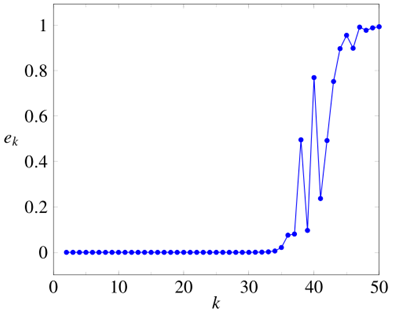
\includegraphics{qr-matlab-error.png}
        
    \end{figure}

    图中显示了 $ q_{k} $ 与前面列之间的正交性的偏差:

    $$
    e_{k}=\max _{1 \leq i<k}\left|q_{i}^{T} q_{k}\right|, \quad k=2, \ldots, n
    $$

    失去正交性是由于\textbf{浮点数存储的舍入误差}。
\end{example}

\section{Householder Algorithm}

Householder算法是QR分解常用的算法(MATLAB和Julia中的qr函数)。与Gram-Schmidt相比,对舍入误差更有鲁棒性。

Householder算法计算一个 “完整的” QR因数分解:
$$ A=\left[\begin{array}{ll}Q & \tilde{Q}\end{array}\right]\left[\begin{array}{l}R \\ 0\end{array}\right], \quad\left[\begin{array}{ll}Q & \tilde{Q}\end{array}\right]  是正交的矩阵$$

\begin{proof}
    $$
    \begin{aligned}
        A&=\left[\begin{array}{ll}Q & \tilde{Q}\end{array}\right]\left[\begin{array}{l}R \\ 0\end{array}\right]\\
        &=QR + \tilde{Q} 0 \\ 
        & = QR
    \end{aligned}
    $$
\end{proof}

完整的Q因子被构造成正交矩阵的乘积:
$$
\left[\begin{array}{ll}
Q & \tilde{Q}
\end{array}\right]=H_{1} H_{2} \cdots H_{n}
$$
每个 $ H_{i} \in \mathbb{R}^{m \times m} $ 是对称的正交的 “反射算子” (reflector)。


\subsection{反射算子}

\begin{theorem}
    $ H=I-2 v v^{T} $, 其中 $ \|v\|_{2}=1 $, $ H x $ 是 $ x $ 关于超平面 $ \left\{u \mid v^{T} u=0\right\} $ 反对称.

    $ H $ 是对称的 
    $$ H^{T}=H $$

$ H $ 是正交的 
$$ H^{T} H=I $$
\end{theorem}
    

\tikzset{every picture/.style={line width=0.75pt}} %set default line width to 0.75pt        



\tikzset{every picture/.style={line width=0.75pt}} %set default line width to 0.75pt        

\begin{tikzpicture}[x=0.75pt,y=0.75pt,yscale=-1,xscale=1]
%uncomment if require: \path (0,300); %set diagram left start at 0, and has height of 300

%Shape: Parallelogram [id:dp7838939596356449] 
\draw  [color={rgb, 255:red, 0; green, 0; blue, 0 }  ,draw opacity=0 ][fill={rgb, 255:red, 213; green, 213; blue, 213 }  ,fill opacity=1 ] (386.97,225.43) -- (240.09,293.42) -- (240.13,95.65) -- (387,27.67) -- cycle ;
%Straight Lines [id:da6147749821862796] 
\draw [color={rgb, 255:red, 109; green, 180; blue, 232 }  ,draw opacity=1 ][line width=2.25]    (314,185.67) -- (313.74,121.96) ;
\draw [shift={(313.72,116.96)}, rotate = 449.76] [fill={rgb, 255:red, 109; green, 180; blue, 232 }  ,fill opacity=1 ][line width=0.08]  [draw opacity=0] (14.29,-6.86) -- (0,0) -- (14.29,6.86) -- cycle    ;
%Straight Lines [id:da41583656892756826] 
\draw [color={rgb, 255:red, 245; green, 166; blue, 35 }  ,draw opacity=1 ][line width=1.5]  [dash pattern={on 1.69pt off 2.76pt}]  (314,185.67) -- (136,118.67) ;
%Straight Lines [id:da16926502578383218] 
\draw [color={rgb, 255:red, 245; green, 166; blue, 35 }  ,draw opacity=1 ][line width=2.25]    (242,158.67) -- (140.68,120.43) ;
\draw [shift={(136,118.67)}, rotate = 380.66999999999996] [fill={rgb, 255:red, 245; green, 166; blue, 35 }  ,fill opacity=1 ][line width=0.08]  [draw opacity=0] (14.29,-6.86) -- (0,0) -- (14.29,6.86) -- cycle    ;
%Straight Lines [id:da9973542879627482] 
\draw [color={rgb, 255:red, 252; green, 132; blue, 147 }  ,draw opacity=1 ][line width=2.25]    (314,185.67) -- (486.78,117.1) ;
\draw [shift={(491.43,115.25)}, rotate = 518.35] [fill={rgb, 255:red, 252; green, 132; blue, 147 }  ,fill opacity=1 ][line width=0.08]  [draw opacity=0] (14.29,-6.86) -- (0,0) -- (14.29,6.86) -- cycle    ;
%Straight Lines [id:da33840798922577653] 
\draw [color={rgb, 255:red, 161; green, 206; blue, 94 }  ,draw opacity=1 ][line width=1.5]  [dash pattern={on 1.69pt off 2.76pt}]  (314,185.67) -- (135,183.96) ;
%Straight Lines [id:da7106398441661397] 
\draw [color={rgb, 255:red, 161; green, 206; blue, 94 }  ,draw opacity=1 ][line width=2.25]    (242,184.96) -- (140,184.01) ;
\draw [shift={(135,183.96)}, rotate = 360.53999999999996] [fill={rgb, 255:red, 161; green, 206; blue, 94 }  ,fill opacity=1 ][line width=0.08]  [draw opacity=0] (14.29,-6.86) -- (0,0) -- (14.29,6.86) -- cycle    ;
%Straight Lines [id:da3197102975021888] 
\draw [color={rgb, 255:red, 161; green, 206; blue, 94 }  ,draw opacity=1 ][line width=2.25]    (314,185.67) -- (485.43,180.69) ;
\draw [shift={(490.43,180.55)}, rotate = 538.3399999999999] [fill={rgb, 255:red, 161; green, 206; blue, 94 }  ,fill opacity=1 ][line width=0.08]  [draw opacity=0] (14.29,-6.86) -- (0,0) -- (14.29,6.86) -- cycle    ;
%Straight Lines [id:da07789590448724115] 
\draw  [dash pattern={on 4.5pt off 4.5pt}]  (136,118.67) -- (135,183.96) ;
%Straight Lines [id:da5486690595919534] 
\draw  [dash pattern={on 4.5pt off 4.5pt}]  (313.72,116.96) -- (136,118.67) ;
%Straight Lines [id:da1919773551202424] 
\draw  [dash pattern={on 4.5pt off 4.5pt}]  (491.43,115.25) -- (313.72,116.96) ;
%Straight Lines [id:da06488229558680647] 
\draw  [dash pattern={on 4.5pt off 4.5pt}]  (491.43,115.25) -- (490.43,180.55) ;
%Straight Lines [id:da5187220488118582] 
\draw [color={rgb, 255:red, 65; green, 117; blue, 5 }  ,draw opacity=1 ][line width=2.25]    (314,185.67) -- (397.22,183.25) ;
\draw [shift={(402.22,183.11)}, rotate = 538.3399999999999] [fill={rgb, 255:red, 65; green, 117; blue, 5 }  ,fill opacity=1 ][line width=0.08]  [draw opacity=0] (14.29,-6.86) -- (0,0) -- (14.29,6.86) -- cycle    ;

% Text Node
\draw (108,107.4) node [anchor=north west][inner sep=0.75pt]    {$\boldsymbol{Hx}$};
% Text Node
\draw (307,97.4) node [anchor=north west][inner sep=0.75pt]    {$u$};
% Text Node
\draw  [color={rgb, 255:red, 12; green, 12; blue, 12 }  ,draw opacity=0 ][fill={rgb, 255:red, 247; green, 140; blue, 105 }  ,fill opacity=1 ]  (286,73) .. controls (286,70.24) and (288.24,68) .. (291,68) -- (346,68) .. controls (348.76,68) and (351,70.24) .. (351,73) -- (351,89) .. controls (351,91.76) and (348.76,94) .. (346,94) -- (291,94) .. controls (288.24,94) and (286,91.76) .. (286,89) -- cycle  ;
\draw (289,72) node [anchor=north west][inner sep=0.75pt]   [align=left] {$\displaystyle \boldsymbol{Hu=u}$};
% Text Node
\draw (87,196.4) node [anchor=north west][inner sep=0.75pt]    {$\boldsymbol{-c_{1} v=H( c_{1} v)}$};
% Text Node
\draw  [color={rgb, 255:red, 0; green, 0; blue, 0 }  ,draw opacity=0 ][fill={rgb, 255:red, 247; green, 140; blue, 105 }  ,fill opacity=1 ]  (490,86) .. controls (490,83.24) and (492.24,81) .. (495,81) -- (579,81) .. controls (581.76,81) and (584,83.24) .. (584,86) -- (584,102) .. controls (584,104.76) and (581.76,107) .. (579,107) -- (495,107) .. controls (492.24,107) and (490,104.76) .. (490,102) -- cycle  ;
\draw (493,85.4) node [anchor=north west][inner sep=0.75pt]    {$\boldsymbol{x=u+c_{1} v}$};
% Text Node
\draw  [color={rgb, 255:red, 0; green, 0; blue, 0 }  ,draw opacity=0 ][fill={rgb, 255:red, 247; green, 140; blue, 105 }  ,fill opacity=1 ]  (365,213) .. controls (365,210.24) and (367.24,208) .. (370,208) -- (428,208) .. controls (430.76,208) and (433,210.24) .. (433,213) -- (433,229) .. controls (433,231.76) and (430.76,234) .. (428,234) -- (370,234) .. controls (367.24,234) and (365,231.76) .. (365,229) -- cycle  ;
\draw (368,212.4) node [anchor=north west][inner sep=0.75pt]    {$\boldsymbol{v}^{T}\boldsymbol{u} =0$};
% Text Node
\draw (483,183.4) node [anchor=north west][inner sep=0.75pt]    {$\boldsymbol{c_{1} v} ,\boldsymbol{c_{1} =v}^{T}\boldsymbol{x}$};
% Text Node
\draw (396,187.4) node [anchor=north west][inner sep=0.75pt]    {$\boldsymbol{v}$};


\end{tikzpicture}

\begin{proof}
    $$\begin{aligned}
        Hv &= (I-2 v v^{T}) (c_1 v) \\
        &= c_1 v - 2 v v^T c_1 v \\
        & = c_1 v - 2 c_1 v v^T v \\
        & = -c_1 v
    \end{aligned}$$

    $$\begin{aligned}
        Hu &= (I - 2 v v^T) u \\
        &= u - 2 v v^T u \\
        & = u \quad (v^T u = 0) 
    \end{aligned}$$

    $$\begin{aligned}
        Hx &= H(u + c_1v) \\
        &= u - c_1 v \\
        &= x - 2(v^Tx)v
    \end{aligned}$$
\end{proof}

矩阵向量积 $ H x $ 能化简为:
$$
H x=x-2\left(v^{T} x\right) v
$$

\subsubsection{$Hx$的算法复杂度}

\begin{theorem}
    如果 $ v $ 和 $ x $ 的长度是 $ p $, 复杂度是 $ 4 p $ flops 。
\end{theorem}


\subsection{构造反射算子}

给定非零p维向量 $ y=\left(y_{1}, y_{2}, \ldots, y_{p}\right) $, 定义

\begin{definition}
    $$w=\left[\begin{array}{c}
        y_{1}+\operatorname{sign}\left(y_{1}\right)\|y\|_{2} \\
        y_{2} \\
        \vdots \\
        y_{p}
        \end{array}\right]$$

    $$v=\frac{1}{\|w\|_{2}} w$$

    $\operatorname{sign}(x)$ 是符号函数, $\operatorname{sign}(0)=0$。
\end{definition}

\begin{theorem}
    向量 $ W $ 满足 $$ \|w\|_{2}^{2}=2 y^{T} w $$
\end{theorem}

$$
\begin{aligned}
    \|w\|_{2}^{2}&=w^{T} w\\
    &=2\left(\|y\|_{2}^{2}+\left|y_{1}\right|\|y\|_{2}\right)\\
    &=2 y^{T}\left(y+\operatorname{sign}\left(y_{1}\right)\|y\|_{2} e_{1}\right)\\
    &=2 y^{T} w 
\end{aligned}
$$

\begin{theorem}
    $$ H=I-2 \frac{w w^{T}}{\|w\|_{2}^{2}} $$
\end{theorem}

\begin{proof}
    $$ H=I-2 v v^{T}=I-2 \frac{w w^{T}}{\|w\|_{2}^{2}} \quad(v=\frac{1}{\|w\|_{2}} w) $$
\end{proof}

\begin{theorem}
    反射算子 $ H=I-2 v v^{T}=I-2 \frac{w w^{T}}{\|w\|_{2}^{2}} $ 将 $ y $ 映射为

   $$ H y = \left[\begin{array}{c}-\operatorname{sign}\left(y_{1}\right)\|y\|_{2} \\ 0 \\ \vdots \\ 0\end{array}\right] $$
\end{theorem}


\begin{proof}
    $$ 
\begin{aligned}
    H y&=y-\frac{2\left(w^{T} y\right)}{\|w\|_{2}^{2}} w\\
    &=y-w\\
    &=-\operatorname{sign}\left(y_{1}\right)\|y\|_{2} e_{1}\\
    &=\left[\begin{array}{c}-\operatorname{sign}\left(y_{1}\right)\|y\|_{2} \\ 0 \\ \vdots \\ 0\end{array}\right]
\end{aligned}
 $$
\end{proof}

即只保留一个元素的值,其余元素的值变为0. 又因为$H$是正交、对称的,它与向量正交化有一定联系。

\subsubsection{构造的反射算子几何意义}



\tikzset{every picture/.style={line width=0.75pt}} %set default line width to 0.75pt        



\tikzset{every picture/.style={line width=0.75pt}} %set default line width to 0.75pt        

\begin{tikzpicture}[x=0.75pt,y=0.75pt,yscale=-1,xscale=1]
%uncomment if require: \path (0,300); %set diagram left start at 0, and has height of 300

%Straight Lines [id:da029865045800250956] 
\draw    (118.48,198.47) -- (513.53,197.71) ;
%Straight Lines [id:da7648219943630132] 
\draw    (249.95,81.42) -- (422.95,297.42) ;
%Straight Lines [id:da0029727641306782626] 
\draw [color={rgb, 255:red, 252; green, 132; blue, 147 }  ,draw opacity=1 ][line width=2.25]    (344.25,197.82) -- (370.82,84.25) ;
\draw [shift={(371.96,79.38)}, rotate = 463.17] [fill={rgb, 255:red, 252; green, 132; blue, 147 }  ,fill opacity=1 ][line width=0.08]  [draw opacity=0] (14.29,-6.86) -- (0,0) -- (14.29,6.86) -- cycle    ;
%Straight Lines [id:da8143455838821552] 
\draw [color={rgb, 255:red, 245; green, 166; blue, 35 }  ,draw opacity=1 ][line width=2.25]    (344.25,197.82) -- (228.57,198.09) ;
\draw [shift={(223.57,198.11)}, rotate = 359.87] [fill={rgb, 255:red, 245; green, 166; blue, 35 }  ,fill opacity=1 ][line width=0.08]  [draw opacity=0] (14.29,-6.86) -- (0,0) -- (14.29,6.86) -- cycle    ;
%Straight Lines [id:da703987286749107] 
\draw  [dash pattern={on 4.5pt off 4.5pt}]  (297.77,138.74) -- (223.57,198.11) ;
%Straight Lines [id:da00886805291354964] 
\draw  [dash pattern={on 4.5pt off 4.5pt}]  (371.96,79.38) -- (297.77,138.74) ;
%Straight Lines [id:da1380735800367292] 
\draw [color={rgb, 255:red, 152; green, 195; blue, 245 }  ,draw opacity=1 ][line width=2.25]    (223.57,198.11) -- (368.05,82.5) ;
\draw [shift={(371.96,79.38)}, rotate = 501.34] [fill={rgb, 255:red, 152; green, 195; blue, 245 }  ,fill opacity=1 ][line width=0.08]  [draw opacity=0] (14.29,-6.86) -- (0,0) -- (14.29,6.86) -- cycle    ;

% Text Node
\draw (302.81,99.57) node [anchor=north west][inner sep=0.75pt]    {$w$};
% Text Node
\draw (159,208.4) node [anchor=north west][inner sep=0.75pt]    {$-\operatorname{sign}( y_{1}) \| y\| e_{1}$};
% Text Node
\draw (360.24,141.91) node [anchor=north west][inner sep=0.75pt]  [rotate=-357.61]  {$y$};
% Text Node
\draw (455,175) node [anchor=north west][inner sep=0.75pt]   [align=left] {坐标轴};
% Text Node
\draw (394,237) node [anchor=north west][inner sep=0.75pt]   [align=left] {超平面$\displaystyle \left\{x|w^{T} x=0\right\}$};


\end{tikzpicture}

关于超平面 $ \left\{x \mid w^{T} x=0\right\} $, 其法向量:
$$
v=\frac{w}{\|w\|_{2}}, w=y+\operatorname{sign}\left(y_{1}\right)\|y\|_{2} e_{1}
$$
反射算子$H$将 $ y $ 映射到向量 $ -\operatorname{sign}\left(y_{1}\right)\|y\|_{2} e_{1} $ 。

\subsection{Householder三角化}

计算反射算子 $ H_{1}, \ldots, H_{n} $ 将A简化为上三角矩阵形式:
$$
H_{n} H_{n-1} \cdots H_{1} A=\left[\begin{array}{l}
R \\
0
\end{array}\right]
$$

第k个步骤之后,矩阵 $ H_{k} H_{k-1} \ldots H_{1} A $ 具有以下结构

\tikzset{every picture/.style={line width=0.75pt}} %set default line width to 0.75pt        
对于 $ i>j $ 和 $ j \leq k $, 第 $ \mathrm{i}, \mathrm{j} $ 个位置的元素为零。

\begin{tikzpicture}[x=0.75pt,y=0.75pt,yscale=-1,xscale=1]
%uncomment if require: \path (0,300); %set diagram left start at 0, and has height of 300

%Shape: Rectangle [id:dp6272763265145869] 
\draw  [fill={rgb, 255:red, 189; green, 189; blue, 189 }  ,fill opacity=1 ] (313,30) -- (453.39,30) -- (453.39,248.71) -- (313,248.71) -- cycle ;
%Shape: Rectangle [id:dp1811444148627901] 
\draw  [color={rgb, 255:red, 0; green, 0; blue, 0 }  ,draw opacity=0 ][fill={rgb, 255:red, 245; green, 166; blue, 35 }  ,fill opacity=1 ] (313,95.38) -- (383,95.38) -- (383,248.71) -- (313,248.71) -- cycle ;
%Shape: Right Triangle [id:dp6024983200469929] 
\draw  [color={rgb, 255:red, 0; green, 0; blue, 0 }  ,draw opacity=0 ][fill={rgb, 255:red, 245; green, 166; blue, 35 }  ,fill opacity=1 ] (313,29.38) -- (383,95.38) -- (313,95.38) -- cycle ;

%Straight Lines [id:da17687674689557986] 
\draw    (466.39,38) -- (466.39,92.38) ;
\draw [shift={(466.39,95.38)}, rotate = 270] [fill={rgb, 255:red, 0; green, 0; blue, 0 }  ][line width=0.08]  [draw opacity=0] (8.93,-4.29) -- (0,0) -- (8.93,4.29) -- cycle    ;
\draw [shift={(466.39,35)}, rotate = 90] [fill={rgb, 255:red, 0; green, 0; blue, 0 }  ][line width=0.08]  [draw opacity=0] (8.93,-4.29) -- (0,0) -- (8.93,4.29) -- cycle    ;
%Straight Lines [id:da19218796013321793] 
\draw    (466.39,98.38) -- (466.39,244.38) ;
\draw [shift={(466.39,247.38)}, rotate = 270] [fill={rgb, 255:red, 0; green, 0; blue, 0 }  ][line width=0.08]  [draw opacity=0] (8.93,-4.29) -- (0,0) -- (8.93,4.29) -- cycle    ;
\draw [shift={(466.39,95.38)}, rotate = 90] [fill={rgb, 255:red, 0; green, 0; blue, 0 }  ][line width=0.08]  [draw opacity=0] (8.93,-4.29) -- (0,0) -- (8.93,4.29) -- cycle    ;
%Straight Lines [id:da4247865332087235] 
\draw    (318.39,257.97) -- (379.39,257.41) ;
\draw [shift={(382.39,257.38)}, rotate = 539.47] [fill={rgb, 255:red, 0; green, 0; blue, 0 }  ][line width=0.08]  [draw opacity=0] (8.93,-4.29) -- (0,0) -- (8.93,4.29) -- cycle    ;
\draw [shift={(315.39,258)}, rotate = 359.47] [fill={rgb, 255:red, 0; green, 0; blue, 0 }  ][line width=0.08]  [draw opacity=0] (8.93,-4.29) -- (0,0) -- (8.93,4.29) -- cycle    ;
%Straight Lines [id:da09293842736310576] 
\draw    (385.39,257.38) -- (451.39,257.38) ;
\draw [shift={(454.39,257.38)}, rotate = 180] [fill={rgb, 255:red, 0; green, 0; blue, 0 }  ][line width=0.08]  [draw opacity=0] (8.93,-4.29) -- (0,0) -- (8.93,4.29) -- cycle    ;
\draw [shift={(382.39,257.38)}, rotate = 0] [fill={rgb, 255:red, 0; green, 0; blue, 0 }  ][line width=0.08]  [draw opacity=0] (8.93,-4.29) -- (0,0) -- (8.93,4.29) -- cycle    ;

% Text Node
\draw (470.39,55.4) node [anchor=north west][inner sep=0.75pt]    {$k$};
% Text Node
\draw (467.39,163.78) node [anchor=north west][inner sep=0.75pt]    {$m-k$};
% Text Node
\draw (341.39,263.4) node [anchor=north west][inner sep=0.75pt]    {$k$};
% Text Node
\draw (395.39,265.4) node [anchor=north west][inner sep=0.75pt]    {$n-k$};
% Text Node
\draw (160.39,128.4) node [anchor=north west][inner sep=0.75pt]    {$H_{n} H_{n-1} \cdots H_{1} A=$};
% Text Node
\draw (341.39,152.4) node [anchor=north west][inner sep=0.75pt]    {$\boldsymbol{0}$};
% Text Node
\draw (371.39,47) node [anchor=north west][inner sep=0.75pt]   [align=left] {Non-zeros};


\end{tikzpicture}



$$ A=\left[\begin{array}{llllllll}X & X & X & X & X & X & X & X \\ X & X & X & X & X & X & X & X \\ X & X & X & X & X & X & X & X \\ X & X & X & X & X & X & X & X \\ X & X & X & X & X & X & X & X \\ X & X & X & X & X & X & X & X \\ X & X & X & X & X & X & X & X \\ X & X & X & X & X & X & X & X\end{array}\right] $$

在第一次处理之后,第一列只剩下第一个元素不为0.

$$H_1A = A_{1}=\left[\begin{array}{llllllll}X & X & X & X & X & X & X & X \\ 0 & X & X & X & X & X & X & X \\ 0 & X & X & X & X & X & X & X \\ 0 & X & X & X & X & X & X & X \\ 0 & X & X & X & X & X & X & X \\ 0 & X & X & X & X & X & X & X \\ 0 & X & X & X & X & X & X & X \\ 0 & X & X & X & X & X & X & X\end{array}\right] $$

第二次处理对于$H_1A_{2:m, 1:n}$($A_{1_{2:m, 1:n} }  $)进行处理。

$$H_2A_1= A_{2}=\left[\begin{array}{cccccccc}X & X & X & X & X & X & X & X \\ 0 & X & X & X & X & X & X & X \\ 0 & 0 & X & X & X & X & X & X \\ 0 & 0 & X & X & X & X & X & X \\ 0 & 0 & X & X & X & X & X & X \\ 0 & 0 & X & X & X & X & X & X \\ 0 & 0 & X & X & X & X & X & X \\ 0 & 0 & X & X & X & X & X & X\end{array}\right] $$

\begin{theorem}
    第$k$个步骤之后,矩阵 $ H_{k} H_{k-1} \ldots H_{1} A $ 具有以下结构:

对于 $ i>j $ 和 $ j \leq k $, 第 $ \mathrm{i}, \mathrm{j} $ 个位置的元素为零.
\end{theorem}


下面的算法用 $ \left[\begin{array}{l}R \\ 0\end{array}\right] $ 来代替 $ A \in \mathbb{R}^{m \times n} $.



\begin{center}
    \tikzset{every picture/.style={line width=0.75pt}} %set default line width to 0.75pt        

\begin{tikzpicture}[x=0.75pt,y=0.75pt,yscale=-1,xscale=1]
%uncomment if require: \path (0,300); %set diagram left start at 0, and has height of 300

%Shape: Rectangle [id:dp6871792923402225] 
\draw  [fill={rgb, 255:red, 189; green, 189; blue, 189 }  ,fill opacity=1 ] (333,28) -- (473.39,28) -- (473.39,246.71) -- (333,246.71) -- cycle ;
%Shape: Rectangle [id:dp8707939685410495] 
\draw  [color={rgb, 255:red, 0; green, 0; blue, 0 }  ,draw opacity=0 ][fill={rgb, 255:red, 245; green, 166; blue, 35 }  ,fill opacity=1 ] (333,93.38) -- (403,93.38) -- (403,246.71) -- (333,246.71) -- cycle ;
%Shape: Right Triangle [id:dp15297612966191965] 
\draw  [color={rgb, 255:red, 0; green, 0; blue, 0 }  ,draw opacity=0 ][fill={rgb, 255:red, 245; green, 166; blue, 35 }  ,fill opacity=1 ] (333,27.38) -- (403,93.38) -- (333,93.38) -- cycle ;

%Straight Lines [id:da37642223834770605] 
\draw    (486.39,36) -- (486.39,90.38) ;
\draw [shift={(486.39,93.38)}, rotate = 270] [fill={rgb, 255:red, 0; green, 0; blue, 0 }  ][line width=0.08]  [draw opacity=0] (8.93,-4.29) -- (0,0) -- (8.93,4.29) -- cycle    ;
\draw [shift={(486.39,33)}, rotate = 90] [fill={rgb, 255:red, 0; green, 0; blue, 0 }  ][line width=0.08]  [draw opacity=0] (8.93,-4.29) -- (0,0) -- (8.93,4.29) -- cycle    ;
%Straight Lines [id:da1511742331917798] 
\draw    (486.39,96.38) -- (486.39,242.38) ;
\draw [shift={(486.39,245.38)}, rotate = 270] [fill={rgb, 255:red, 0; green, 0; blue, 0 }  ][line width=0.08]  [draw opacity=0] (8.93,-4.29) -- (0,0) -- (8.93,4.29) -- cycle    ;
\draw [shift={(486.39,93.38)}, rotate = 90] [fill={rgb, 255:red, 0; green, 0; blue, 0 }  ][line width=0.08]  [draw opacity=0] (8.93,-4.29) -- (0,0) -- (8.93,4.29) -- cycle    ;
%Straight Lines [id:da9300057482807336] 
\draw    (338.39,255.97) -- (399.39,255.41) ;
\draw [shift={(402.39,255.38)}, rotate = 539.47] [fill={rgb, 255:red, 0; green, 0; blue, 0 }  ][line width=0.08]  [draw opacity=0] (8.93,-4.29) -- (0,0) -- (8.93,4.29) -- cycle    ;
\draw [shift={(335.39,256)}, rotate = 359.47] [fill={rgb, 255:red, 0; green, 0; blue, 0 }  ][line width=0.08]  [draw opacity=0] (8.93,-4.29) -- (0,0) -- (8.93,4.29) -- cycle    ;
%Straight Lines [id:da8104730881110522] 
\draw    (405.39,255.38) -- (471.39,255.38) ;
\draw [shift={(474.39,255.38)}, rotate = 180] [fill={rgb, 255:red, 0; green, 0; blue, 0 }  ][line width=0.08]  [draw opacity=0] (8.93,-4.29) -- (0,0) -- (8.93,4.29) -- cycle    ;
\draw [shift={(402.39,255.38)}, rotate = 0] [fill={rgb, 255:red, 0; green, 0; blue, 0 }  ][line width=0.08]  [draw opacity=0] (8.93,-4.29) -- (0,0) -- (8.93,4.29) -- cycle    ;
%Shape: Rectangle [id:dp3957948372583875] 
\draw  [color={rgb, 255:red, 0; green, 0; blue, 0 }  ,draw opacity=0 ][fill={rgb, 255:red, 255; green, 147; blue, 147 }  ,fill opacity=1 ] (403,93.38) -- (473.39,93.38) -- (473.39,246.42) -- (403,246.42) -- cycle ;
%Straight Lines [id:da6423678439002216] 
\draw [color={rgb, 255:red, 139; green, 87; blue, 42 }  ,draw opacity=1 ][line width=3]    (403,93.38) -- (403,246.42) ;
%Straight Lines [id:da15094884239960105] 
\draw [color={rgb, 255:red, 139; green, 87; blue, 42 }  ,draw opacity=1 ][line width=2.25]  [dash pattern={on 6.75pt off 4.5pt}]  (403,93.38) -- (473.39,93.38) ;
%Straight Lines [id:da6820341280353248] 
\draw [color={rgb, 255:red, 139; green, 87; blue, 42 }  ,draw opacity=1 ][line width=2.25]  [dash pattern={on 6.75pt off 4.5pt}]  (473.39,93.38) -- (473.39,246.42) ;
%Straight Lines [id:da3968465055227026] 
\draw [color={rgb, 255:red, 139; green, 87; blue, 42 }  ,draw opacity=1 ][line width=2.25]  [dash pattern={on 6.75pt off 4.5pt}]  (403,246.42) -- (473.39,246.42) ;

% Text Node
\draw (490.39,53.4) node [anchor=north west][inner sep=0.75pt]    {$k$};
% Text Node
\draw (487.39,161.78) node [anchor=north west][inner sep=0.75pt]    {$m-k$};
% Text Node
\draw (361.39,261.4) node [anchor=north west][inner sep=0.75pt]    {$k$};
% Text Node
\draw (415.39,263.4) node [anchor=north west][inner sep=0.75pt]    {$n-k$};
% Text Node
\draw (361.39,150.4) node [anchor=north west][inner sep=0.75pt]    {$\boldsymbol{0}$};
% Text Node
\draw (387.39,49) node [anchor=north west][inner sep=0.75pt]   [align=left] {Non-zeros};


\end{tikzpicture}
\end{center}


\begin{algorithm}[htbp]
    \caption{Householder算法}

    \For(){$k$ in $1:n$}{
        令 $ y=A_{k: m, k} \in \mathbb{R}^{m-k+1} $, 计算向量 $ v_{k} $
    $$ w=y+\operatorname{sign}\left(y_{1}\right)\|y\| e_{1}, \quad v_{k}=\frac{1}{\|w\|} w $$\;
    将 $ A_{k: m, k: n} \in \mathbb{R}^{(m-k+1) \times(n-k+1)} $ 与反射矩阵 $ I-2 v_{k} v_{k}^{T} $ 相乘
    $$ A_{k: m, k: n}:=A_{k: m, k: n}-2 v_{k}\left(v_{k}^{T} A_{k: m, k: n}\right) $$\;

    }
    
\end{algorithm}

\begin{proof}
    在步骤2中,将 $ A_{k: m, k: n} $ 与反射算子 $ I-2 v_{k} v_{k}^{T} $ 相乘

$$ \left(I-2 v_{k} v_{k}^{T}\right) A_{k: m, k: n}=A_{k: m, k: n}-2 v_{k}\left(v_{k}^{T} A_{k: m, k: n}\right) $$

等价于用 $ H_{k} \in \mathbb{R}^{m \times m} $ 乘以 $ A $

$$ H_{k}=\left[\begin{array}{cc}I & 0 \\ 0 & I-2 v_{k} v_{k}^{T}\end{array}\right]=I-2\left[\begin{array}{c}0 \\ v_{k}\end{array}\right]\left[\begin{array}{l}0 \\ v_{k}\end{array}\right]^{T} $$

算法将下列矩阵来代替 $ A $
$$
\left[\begin{array}{c}
R \\
0
\end{array}\right]
$$

返回向量 $ v_{1}, \ldots, v_{n} $, 其中 $ v_{k} $ 的长度为 $ m-k+1 $ 。
\end{proof}


\subsection{An Example for Householder Algorithm}

\begin{problem}
    $$ A=\left[\begin{array}{rrr}-1 & -1 & 1 \\ 1 & 3 & 3 \\ -1 & -1 & 5 \\ 1 & 3 & 7\end{array}\right]=H_{1} H_{2} H_{3}\left[\begin{array}{l}R \\ 0\end{array}\right] $$

    计算反射算子 $ H_{1}, H_{2}, H_{3} $ 来将矩阵$A$三角化

    $$ H_{3} H_{2} H_{1} A=\left[\begin{array}{ccc}R_{11} & R_{12} & R_{13} \\ 0 & R_{22} & R_{23} \\ 0 & 0 & R_{33} \\ 0 & 0 & 0\end{array}\right] $$

    $R$的第一列:计算将$A$的第一列映射到$e_1$乘积的反射算子

    $$
y=\left[\begin{array}{r}
-1 \\
1 \\
-1 \\
1
\end{array}\right], \quad w=y-\|y\|_{2} e_{1}=\left[\begin{array}{r}
-3 \\
1 \\
-1 \\
1
\end{array}\right], \quad v_{1}=\frac{1}{\|w\|_{2}} w=\frac{1}{2 \sqrt{3}}\left[\begin{array}{r}
-3 \\
1 \\
-1 \\
1
\end{array}\right]
$$

用 $I-2 v_{1} v_{1}^{T}$ 和$A$的乘积代替$A$:
$$
A:=\left(I-2 v_{1} v_{1}^{T}\right) A=\left[\begin{array}{ccc}
2 & 4 & 2 \\
0 & 4 / 3 & 8 / 3 \\
0 & 2 / 3 & 16 / 3 \\
0 & 4 / 3 & 20 / 3
\end{array}\right]
$$

$R$的第二列:计算将 $ A_{2: 4,2} $ 映射到 $ e_{1} $ 乘积的反射算子

$$y=\left[\begin{array}{l}
    4 / 3 \\
    2 / 3 \\
    4 / 3
    \end{array}\right], \quad w=y+\|y\|_{2} e_{1}=\left[\begin{array}{r}
    10 / 3 \\
    2 / 3 \\
    4 / 3
    \end{array}\right], \quad v_{2}=\frac{1}{\|w\|_{2}} w=\frac{1}{\sqrt{30}}\left[\begin{array}{l}
    5 \\
    1 \\
    2
    \end{array}\right]
$$

用 $I-2 v_{2} v_{2}^{T}$ 和 $A_{2: 4,2: 3}$ 的乘积代替 $A_{2: 4,2: 3}$ :
$$
A:=\left[\begin{array}{cc}
1 & 0 \\
0 & I-2 v_{2} v_{2}^{T}
\end{array}\right] A=\left[\begin{array}{rrr}
2 & 4 & 2 \\
0 & -2 & -8 \\
0 & 0 & 16 / 5 \\
0 & 0 & 12 / 5
\end{array}\right]
$$

$R$的第三列:计算将$ A_{3: 4,3} $映射到$e_1$乘积的反射算子

$$y=\left[\begin{array}{l}
    16 / 5 \\
    12 / 5
    \end{array}\right], \quad w=y+\|y\|_{2} e_{1}=\left[\begin{array}{c}
    36 / 5 \\
    12 / 5
    \end{array}\right], \quad v_{3}=\frac{1}{\|w\|_{2}} w=\frac{1}{\sqrt{10}}\left[\begin{array}{l}
    3 \\
    1
    \end{array}\right]
$$

用 $I-2 v_{3} v_{3}^{T}$ 和 $A_{3: 4,3}$ 的乘积代替 $A_{3: 4,3}$ :
$$
A:=\left[\begin{array}{cc}
I & 0 \\
0 & I-2 v_{3} v_{3}^{T}
\end{array}\right] A=\left[\begin{array}{rrr}
2 & 4 & 2 \\
0 & -2 & -8 \\
0 & 0 & -4 \\
0 & 0 & 0
\end{array}\right]
$$


    $$ \begin{aligned} H_{3} H_{2} H_{1} A &=\left[\begin{array}{cc}I_{2} & 0 \\ 0 & I_{2}-2 v_{3} v_{3}^{T}\end{array}\right]\left[\begin{array}{cc}I_{1} & 0 \\ 0 & I_{3}-2 v_{2} v_{2}^{T}\end{array}\right]\left(I_{4}-2 v_{1} v_{1}^{T}\right) A \\ &=\left[\begin{array}{cc}I_{2} & 0 \\ 0 & I_{2}-2 v_{3} v_{3}^{T}\end{array}\right]\left[\begin{array}{cc}I_{1} & 0 \\ 0 & I_{3}-2 v_{2} v_{2}^{T}\end{array}\right]\left[\begin{array}{ccc}2 & 4 & 2 \\ 0 & 4 / 3 & 8 / 3 \\ 0 & 2 / 3 & 16 / 3 \\ 0 & 4 / 3 & 20 / 3\end{array}\right] \\ &=\left[\begin{array}{cc}I_{2} & 0 \\ 0 & I_{2}-2 v_{3} v_{3}^{T}\end{array}\right]\left[\begin{array}{rrr}2 & 4 & 2 \\ 0 & -2 & -8 \\ 0 & 0 & 16 / 5 \\ 0 & 0 & 12 / 5\end{array}\right] \\ &=\left[\begin{array}{rrr}2 & 4 & 2 \\ 0 & -2 & -8 \\ 0 & 0 & -4 \\ 0 & 0 & 0\end{array}\right] \end{aligned} $$
\end{problem}

\subsection{Complexity of Householder Algorithm}

Householder方法第$k$次循环的复杂度:

\begin{itemize}
    \item $ v_{k}^{T} A_{k: m, k: n} $ 的乘积: $ (2(\mathrm{~m}-\mathrm{k}+1)-1)(\mathrm{n}-\mathrm{k}+1) $ flops
    \item $ v_{k} $ 的外积: $ (m-k+1)(n-k+1) $ flops
    \item $ A_{k: m, k: n} $ 的减法: $ (\mathrm{m}-\mathrm{k}+1)(\mathrm{n}-\mathrm{k}+1) $ flops
\end{itemize}

第$k$次循环的总和: $ 4(\mathrm{~m}-\mathrm{k}+1)(\mathrm{n}-\mathrm{k}+1) $ flops

计算 $ R $ 和 $ v_{1}, \ldots, v_{n} $ 的总复杂度

$$ \begin{aligned} \sum_{k=1}^{n} 4(m-k+1)(n-k+2) & \approx \int_{0}^{n} 4(m-t)(n-t+1) d t \\ & \approx 2 m n^{2}-\frac{2}{3} n^{3} \text { flops } \end{aligned} $$

\section{$Q$因子}

Householder算法返回向量 $ v_{1}, \ldots, v_{n} $, 其定义为:

\begin{definition}[ $ v_{1}, \ldots, v_{n} $ 的完整表示]
   $$
\left[\begin{array}{ll}
Q & \tilde{Q}
\end{array}\right]=H_{1} H_{2} \cdots H_{n}
$$ 
\end{definition}

通常不需计算矩阵 $ \left[\begin{array}{ll}Q & \tilde{Q}\end{array}\right] $ 。向量 $ v_{1}, \ldots, v_{n} $ 是 $ \left[\begin{array}{ll}Q & \tilde{Q}\end{array}\right] $ 简单表示(economical representation)。

\begin{theorem}
    $ \left[\begin{array}{ll}Q & \tilde{Q}\end{array}\right] $ 或其转置的乘积可以计算为:
$$
\begin{array}{c}
{\left[\begin{array}{cc}
Q & \tilde{Q}
\end{array}\right] x=H_{1} H_{2} \cdots H_{n} x} \\
{\left[\begin{array}{ll}
Q & \tilde{Q}
\end{array}\right]^{T} y=H_{n} H_{n-1} \cdots H_{1} y}
\end{array}
$$
\end{theorem}

\begin{definition}
    矩阵-向量积 $ H_{k} x $ 定义为:
$$
H_{k} x=\left[\begin{array}{cc}
I_{k-1} & 0 \\
0 & I-2 v_{k} v_{k}^{T}
\end{array}\right]\left[\begin{array}{c}
x_{1: k-1} \\
x_{k: m}
\end{array}\right]=\left[\begin{array}{c}
x_{1: k-1} \\
x_{k: m}-2\left(v_{k}^{T} x_{k: m}\right) v_{k}
\end{array}\right]
$$
\end{definition}

\subsection{矩阵-向量积 $ H_{k} x $算法复杂度}

$ H_{k} x $ 乘积的复杂度为: $ 4(\mathrm{~m}-\mathrm{k}+1) $ flops。

$H_{1} H_{2}, \ldots H_{n} $或其转置的乘积的复杂度为: 

$$ \sum_{k=1}^{n} 4(m-k+1) \approx 4 m n-2 n^{2}  \text{ flops}$$

其复杂度约等于$m \times n$矩阵的矩阵-向量乘积($2mn$ flops)。 
\chapter{LU分解}

\section{Solving Linear Equation Systems}

\subsection{Linear Equation Systems}
\begin{example}
    \begin{equation}
         A\boldsymbol{x} =\boldsymbol{b} \Leftrightarrow { \left\{\begin{matrix}
        x & + & 2y & + & 3z & = & 6\\
        2x & + & 5y & + & 2z & = & 4\\
        6x & - & 3y & + & z & = & 2
        \end{matrix}\right. }
         \end{equation}
\end{example}

见Row Picture,Column Picture的概念。

\subsection{Elimination}

\begin{example}[Elimination]
    Before

        \begin{equation} \left\{\begin{matrix}
        x & - & 2y & = & 1\\
        3x & + & 2y & = & 11
        \end{matrix}\right. \end{equation}
        
        
   
    After
    
    \begin{equation} \left\{\begin{matrix}
        x & - & 2y & = & 1\\
         &  & 8y & = & 8
        \end{matrix}\right. \end{equation}
    

\end{example}

\begin{definition}[Pivot]
    The first nonzero in the row that does elimination. \textbf{Zero is not allowed as a pivot.}
\end{definition}

\begin{definition}[Multiplier]
    (Entry to eliminate) divided by (pivot)
\end{definition}

消元法通过elimination matrices $E$进行消元操作,使得主对角线以下的元素为0. Multiply the $ j^{\text {th }} $ equation by $ \ell_{i j} $ and subtract from the $ i^{\text {th }} $ equation. (This eliminates $ x_{j} $ from equation $ i $.) We need a lot of these simple matrices $ E_{i j} $, one for every nonzero to be eliminated below the main diagonal.

\subsection{消元法的本质}

\begin{definition}[Elementary matrix, Elimination matrix]
    The elementary matrix or elimination matrix $ E_{i j} $ has the extra nonzero entry $ -\ell $ in the $ i, j $ position. Then $ E_{i j} $ subtracts a multiple $ \ell $ of row $ j $ from row $ i $.
\end{definition}

\begin{theorem}
    消元法的本质是

    \begin{equation}Ax= b \Rightarrow EAx = Eb\end{equation}
\end{theorem}

\begin{example}[Inverse of an elimination matrix]
    If $ E $ subtracts 5 times row 1 from row 2 , then $ E^{-1} $ adds 5 times row 1 to row 2 :
$$
\begin{array}{c}
\boldsymbol{E} \text { subtracts } \\
\boldsymbol{E}^{-1} \text { adds }
\end{array} \quad E=\left[\begin{array}{rll}
1 & 0 & 0 \\
-\mathbf{5} & 1 & 0 \\
0 & 0 & 1
\end{array}\right] \quad \text { and } \quad E^{-1}=\left[\begin{array}{lll}
1 & 0 & 0 \\
\mathbf{5} & 1 & 0 \\
0 & 0 & 1
\end{array}\right]
$$
Multiply $ E E^{-1} $ to get the identity matrix $ I $. Also multiply $ E^{-1} E $ to get $ I $. We are adding and subtracting the same 5 times row 1 . If $ A C=I $ then automatically $ C A=I $.
\end{example}

\begin{example}
    Suppose $ F $ subtracts 4 times row 2 from row 3 , and $ F^{-1} $ adds it back:
$$
F=\left[\begin{array}{rrr}
1 & 0 & 0 \\
0 & 1 & 0 \\
0 & -4 & 1
\end{array}\right] \text { and } F^{-1}=\left[\begin{array}{lll}
1 & 0 & 0 \\
0 & 1 & 0 \\
0 & 4 & 1
\end{array}\right] \text {. }
$$

Now multiply $ F $ by the matrix $ E $ in Example 2 to find $ F E $. Also multiply $ E^{-1} $ times $ F^{-1} $ to find $ (F E)^{-1} $. Notice the orders $ F E $ and $ E^{-1} F^{-1} $ !
$$
F E=\left[\begin{array}{rrr}
1 & 0 & 0 \\
-5 & 1 & 0 \\
20 & -4 & 1
\end{array}\right] \quad \text { is inverted by } \quad E^{-1} F^{-1}=\left[\begin{array}{ccc}
1 & 0 & 0 \\
5 & 1 & 0 \\
0 & 4 & 1
\end{array}\right]
$$


\end{example}

The result is beautiful and correct. The product $ F E $ contains  ``20'' but its inverse doesn't. $ E $ subtracts 5 times row 1 from row 2 . Then $ F $ subtracts 4 times the new row 2 (changed by row 1) from row 3 . In this order $ F E $, row 3 feels an effect from row 1 .

In the order $ E^{-1} F^{-1} $, that effect does not happen. First $ F^{-1} $ adds 4 times row 2 to row 3 . After that, $ E^{-1} $ adds 5 times row 1 to row 2 . There is no 20 , because row 3 doesn't change again. In this order $ E^{-1} F^{-1} $, row 3 feels no effect from row 1 .

This is why the next section chooses $ A=L U $, to go back from the triangular $ U $ to $ A $. \textbf{The multipliers fall into place perfectly in the lower triangular $ L $}.

\begin{definition}[Permutation matrices $P$]
    $  P_{i j} $ is the identity matrix with rows $ i $ and $ j $ reversed. When this \term{permutation matrix} $ P_{i j} $ multiplies a matrix, it exchanges rows $ i $ and $ j $.
\end{definition}


\subsection{Computing $A^{-1}$ by Gauss-Jordan Elimination}

\begin{definition}[Augmented matrix]
    \begin{equation} \left[\begin{matrix}
                A & b
            \end{matrix}\right]\end{equation}
\end{definition}

\begin{center}
    Multiply $ \left[\begin{matrix}
                A & I
            \end{matrix}\right]$ by $ A^{-1}$ to get $ \left[\begin{matrix}
                I & A^{-1}
            \end{matrix}\right]$
\end{center}

\begin{remark}
    The inverse exists if and only if elimination produces $n$ pivots. Row exchanges are allowed. Elimination solves $Ax = b$ without explicitly using the matrix $A^{-1}$.
\end{remark}

\begin{remark}
    (Important) Suppose there is a nonzero vector $ x $ such that $ A x=0 . $ Then $ A $ cannot have an inverse. No matrix can bring $ \mathbf{0} $ back to $ \boldsymbol{x} $.

If $ A $ is invertible, then $ A x=0 $ can only have the \textbf{zero solution} $ x=A^{-1} 0=0 $.
\end{remark}


\begin{example}
    \begin{equation} \begin{aligned}\left[\begin{array}{llll}K & e_{1} & e_{2} & e_{3}\end{array}\right] & =\left[\begin{array}{rrrrrr}\mathbf{2} & -\mathbf{1} & \mathbf{0} & 1 & 0 & 0 \\ -\mathbf{1} & \mathbf{2} & -\mathbf{1} & 0 & 1 & 0 \\ \mathbf{0} & -\mathbf{1} & \mathbf{2} & 0 & 0 & 1\end{array}\right] \quad \text { Start Gauss-Jordan on } K                                                  \\ & \rightarrow\left[\begin{array}{rrrrrr}2 & -1 & 0 & 1 & 0 & 0 \\ \mathbf{0} & \frac{3}{2} & -\mathbf{1} & \frac{1}{2} & \mathbf{1} & \mathbf{0} \\ 0 & -1 & 2 & 0 & 0 & 1\end{array}\right] \quad\left(\frac{\mathbf{1}}{\mathbf{2}} \text { row } 1+\text { row 2 }\right) \\ & \rightarrow\left[\begin{array}{rrrrrr}2 & -1 & 0 & 1 & 0 & 0 \\ 0 & \frac{3}{2} & -1 & \frac{1}{2} & 1 & 0 \\ \mathbf{0} & \mathbf{0} & \frac{4}{3} & \frac{1}{3} & \frac{2}{3} & \mathbf{1}\end{array}\right] \quad \left(\frac{\mathbf{2}}{3} \text { row 2 + row 3}\right)\\
               \left(\begin{array}{c}\text { Zero above } \\ \text { third pivot }\end{array}\right) & \rightarrow\left[\begin{array}{rrrrrr}2 & -1 & 0 & 1 & 0 & 0 \\ 0 & \frac{3}{2} & 0 & \frac{3}{4} & \frac{3}{2} & \frac{3}{4} \\ 0 & 0 & \frac{4}{3} & \frac{1}{3} & \frac{2}{3} & 1\end{array}\right] \quad\left(\frac{3}{4} \text{ row } \mathbf{3}+ \text{ row } \mathbf{2}\right) \\
               \left(\begin{array}{l}\text { Zero above } \\ \text { second pivot }\end{array}\right) & \rightarrow\left[\begin{array}{cccccc}2 & 0 & 0 & \frac{3}{2} & 1 & \frac{1}{2} \\ 0 & \frac{3}{2} & 0 & \frac{3}{4} & \frac{3}{2} & \frac{3}{4} \\ 0 & 0 & \frac{4}{3} & \frac{1}{3} & \frac{2}{3} & 1\end{array}\right] \quad\left(\frac{2}{3} \text{ row } 2+ \text{ row }1 \right)
        \end{aligned} \end{equation}


    然后将它变成Reduced echelon form $R$.

   
    \begin{equation} \begin{matrix}
                (\text{divided by }2)                      \\
                \left(\text{divided by }\dfrac{3}{2}\right) \\
                \left(\text{divided by }\dfrac{4}{3}\right)
            \end{matrix}\left[\begin{matrix}
                    1 & 0 & 0 & \dfrac{3}{4} & \dfrac{1}{2} & \dfrac{1}{4} \\
                    0 & 1 & 0 & \dfrac{1}{2} & 1           & \dfrac{1}{2} \\
                    0 & 0 & 1 & \dfrac{1}{4} & \dfrac{1}{2} & \dfrac{3}{4}
                \end{matrix}\right] =\left[\begin{matrix}
                    I & x_{1} & x_{2} & x_{3}
                \end{matrix}\right] =\ \left[\begin{matrix}
                    I & K^{-1}
                \end{matrix}\right]\end{equation}
    


    \begin{enumerate}
        \item $ K $ is symmetric across its main diagonal. Then $ K^{-1} $ is also symmetric.
        \item $ K $ is tridiagonal (only three nonzero diagonals). But $ K^{-1} $ is a dense matrix with no zeros. That is another reason we don't often compute inverse matrices. The inverse of a band matrix is generally a dense matrix.
        \item The product of pivots is $ 2\left(\frac{3}{2}\right)\left(\frac{4}{3}\right)=4 $. This number 4 is the determinant of $ K $. $ K^{-1} $ involves division by the determinant of $ K $.
        \begin{equation} K^{-1}=\frac{1}{4}\left[\begin{array}{lll}3 & 2 & 1 \\ 2 & 4 & 2 \\ 1 & 2 & 3\end{array}\right] \end{equation}
    \end{enumerate}


    This is why an \textbf{invertible matrix} cannot have a \textbf{zero determinant}: we need to \textbf{divide}.

\end{example}

\section{LU分解}

$ \left(E_{32} E_{31} E_{21}\right) A=U \quad $ becomes $ \quad A=\left(E_{21}^{-1} E_{31}^{-1} E_{32}^{-1}\right) U \quad $ which is $ \quad A=L U $

\begin{theorem}
    When a row of $A$ starts with zeros, so does that row of $L$.

    When a column of $A$ starts with zeros, so does that column of $U$.
\end{theorem}

\begin{example}[The key reason why $ A $ equals $ L U$]
    Ask yourself about the pivot rows that are subtracted from lower rows. Are they the original rows of $ A ? $ No, elimination probably changed them.

    Are they rows of $ U ? $ Yes, the pivot rows never change again.

    When computing the third row of $ U $, we subtract multiples of earlier rows of $ U $ (not rows of $ A ! $ ):
    \begin{equation} \text{Row 3 of }  U=(\text{Row 3 of }  A)-\ell_{31}(
        \text{Row 1 of } U)-\ell_{32}(\text{Row 2 of }  of  U) \end{equation}

    Rewrite this equation to see that the row $ \left[\begin{array}{lll}\ell_{31} & \ell_{32} & 1\end{array}\right] $ is multiplying the matrix $ U $ :

    \begin{equation} (\text{Row 3 of } A)=\ell_{31}(\text{Row 1 of }  U)+\ell_{32}(\text{Row 2 of } U)+1(\text{Row 3 of }  U) \end{equation}

    This is exactly row 3 of $ A=L U . $

    That row of $
        L $ holds $ \ell_{31}, \ell_{32}, 1 . $ All rows look like this, whatever the size of $ A $. With no row exchanges, we have $ A=L U $.
\end{example}

\begin{definition}[$A$的LU分解]
    \begin{equation} A=\left(\begin{array}{ccccc}a_{11} & \cdots & a_{1 k} & \cdots & a_{1 n} \\ \vdots & \ddots & \vdots & & \vdots \\ a_{k 1} & \cdots & a_{k k} & \cdots & a_{k n} \\ \vdots & & \vdots & \ddots & \vdots \\ a_{n 1} & \cdots & a_{n k} & \cdots & a_{n n}\end{array}\right) =LU \end{equation}

    where $ L=\left(\begin{array}{cccc}1 & 0 & \cdots & 0 \\ l_{21} & 1 & \ddots & 0 \\ \vdots & \vdots & \ddots & 0 \\ l_{n 1} & l_{n 2} & \cdots & 1\end{array}\right) , U=\left(\begin{array}{cccc}u_{11} & u_{12} & \cdots & u_{1 n} \\ 0 & u_{22} & \cdots & u_{2 n} \\ \vdots & 0 & \ddots & \vdots \\ 0 & 0 & 0 & u_{n n}\end{array}\right) $
\end{definition}

所以
\begin{equation}
    \begin{aligned}
        A & =\left(\begin{array}{ccccc}a_{11} & \cdots & a_{1 r} & \cdots & a_{1 n} \\ \vdots & \ddots & \vdots & & \vdots \\ a_{r 1} & \cdots & a_{r r} & \cdots & a_{r n} \\ \vdots & & \vdots & \ddots & \vdots \\ a_{n 1} & \cdots & a_{n r} & \cdots & a_{n n}\end{array}\right)                                               \\
          & =\left(\begin{array}{ccccc}1 & 0 & 0 & \cdots & 0 \\ \vdots & \ddots & 0 & \ddots & 0 \\ l_{r 1} & \cdots & 1 & \ddots & \vdots \\ \vdots & & \vdots & \ddots & 0 \\ l_{n 1} & \cdots & l_{n r} & \cdots & 1\end{array}\right) \cdot \left(\begin{array}{cccc}u_{11} & u_{12} & \cdots & u_{1 n} \\ 0 & u_{22} & \cdots & u_{2 n} \\ \vdots & 0 & \ddots & \vdots \\ 0 & 0 & 0 & u_{n n}\end{array}\right)
    \end{aligned}
\end{equation}

\begin{remark}
    First point: Every inverse matrix $ E^{-1} $ is lower triangular. Its off-diagonal entry is $ \ell_{i j} $, to undo the subtraction produced by $ -\ell_{i j} . $ The main diagonals of $ E $ and $ E^{-1} $ contain 1's.
\end{remark}

\begin{remark}
    Second point: Equation (2) shows a lower triangular matrix (the product of the $ E_{i j} $ ) multiplying $ A . $ It also shows all the $ E_{i j}^{-1} $ multiplying $ U $ to bring back $ A . $ This lower triangular product of inverses is $ L $.
\end{remark}

One reason for working with the inverses is that we want to factor $ A $, not $ U $. The "inverse form" gives $ A=L U $. Another reason is that we get something extra, almost more than we deserve. This is the third point, showing that $ L $ is exactly right.

\begin{remark}
    Third point: Each multiplier $ \ell_{i j} $ goes directly into its $ i, j $ position-\textbf{unchanged}-in the product of inverses which is $ L $. Usually matrix multiplication will mix up all the numbers. Here that doesn't happen. The order is right for the inverse matrices, to keep the $ \ell $'s unchanged. The reason is given below in equation (2).
Since each $ E^{-1} $ has 1's down its diagonal, the final good point is that $ L $ does too.
\end{remark}

Since each $ E^{-1} $ has 1's down its diagonal, the final good point is that $ L $ does too.

This is \textbf{elimination without row exchanges}. The upper triangular $ U $ has the pivots on its diagonal. The lower triangular $ L $ has all 1 's on its diagonal. \textbf{The multipliers $ \ell_{i j} $ are below the diagonal of $ L $}.

\subsection{$A = LDU$}

$A=LU$是不对称的。但是可以改写为对称形式。

Split $ U $ into $ \left[\begin{array}{cccc}d_{1} & & & \\ & d_{2} & & \\ & & \ddots & \\ & & & d_{n}\end{array}\right]\left[\begin{array}{cccc}1 & u_{12} / d_{1} & u_{13} / d_{1} & \cdot \\ & 1 & u_{23} / d_{2} & \cdot \\ & & \ddots & \vdots \\ & & & 1\end{array}\right] $.

\begin{example}
    
    \begin{equation}(A= LU) \left[\begin{array}{ll}1 & 0 \\ 3 & 1\end{array}\right]\left[\begin{array}{ll}2 & 8 \\ 0 & 5\end{array}\right] \end{equation} 
    
    splits further into
    
    \begin{equation}(A= LDU) \left[\begin{array}{ll}1 & 0 \\ 3 & 1\end{array}\right]\left[\begin{array}{ll}2 & \\ & 5\end{array}\right]\left[\begin{array}{ll}1 & 4 \\ 0 & 1\end{array}\right] \end{equation}.
    
\end{example}

\begin{theorem}
    当$A$是对称矩阵的时候,且消元的时候不需要行交换:

    \begin{equation}S = LDL^T\end{equation}
\end{theorem}


\begin{example}
    \begin{equation} \left[\begin{array}{ll}1 & 2 \\ 2 & 7\end{array}\right]=\left[\begin{array}{ll}\mathbf{1} & 0 \\ \mathbf{2} & \mathbf{1}\end{array}\right] \quad\left[\begin{array}{ll}1 & 0 \\ 0 & 3\end{array}\right] \quad\left[\begin{array}{ll}\mathbf{1} & \mathbf{2} \\ 0 & \mathbf{1}\end{array}\right] \end{equation}
\end{example}


\subsection{$L$、$U$矩阵的性质}

回顾矩阵乘法的定义

\begin{definition}[矩阵乘法]
    设矩阵 $ A \in \mathfrak{R}^{m \times p}, B \in \mathfrak{R}^{p \times n} $,那么矩阵$A$与$B$的乘积, 记 作C $ =A B $ ,  则矩阵 $ C \in \mathfrak{R}^{m \times n} $ 的第 $i$行第 $ j $ 列元素 $ C_{i j} $


    \begin{equation}
{C}_{i j}=\sum_{k=1}^{p} A_{i k} B_{k j}
\end{equation}
\end{definition}

对于$L$、$U$有

\begin{theorem}
    $ A $ 的第一行元素 $ a_{1 j} $ 为
    \begin{equation}
        a_{1 j}=u_{1 j}, j=1, \cdots, n
    \end{equation}
\end{theorem}

\begin{corollary}
    $ U $ 的第一行元素 $ u_{1 j} $ 为
    \begin{equation}
        u_{1 j}=a_{1 j}, j=1, \cdots, n
    \end{equation}
\end{corollary}

\begin{proof}
    \begin{equation} \begin{aligned}A & =\left(\begin{array}{ c c c c c }
                \boldsymbol{\textcolor[rgb]{0.72,0.33,0.31}{a_{11}}} & \boldsymbol{\textcolor[rgb]{0.72,0.33,0.31}{\cdots }} & \boldsymbol{\textcolor[rgb]{0.72,0.33,0.31}{a_{1r}}} & \boldsymbol{\textcolor[rgb]{0.72,0.33,0.31}{\cdots }} & \boldsymbol{\textcolor[rgb]{0.72,0.33,0.31}{a_{1n}}} \\
                \vdots                                               & \ddots                                                & \vdots                                               &                                                       & \vdots                                               \\
                a_{r1}                                               & \cdots                                                & a_{rr}                                               & \cdots                                                & a_{rn}                                               \\
                \vdots                                               &                                                       & \vdots                                               & \ddots                                                & \vdots                                               \\
                a_{n1}                                               & \cdots                                                & a_{nr}                                               & \cdots                                                & a_{nn}
            \end{array}\right)
               \\ &=\left(\begin{array}{ c c c c c }
                \boldsymbol{\textcolor[rgb]{0.72,0.33,0.31}{1}} & 0      & 0      & \cdots & 0      \\
                \vdots                                          & \ddots & 0      & \ddots & 0      \\
                l_{r1}                                          & \cdots & 1      & \cdots & \vdots \\
                \vdots                                          & \ddots & \vdots & \ddots & 0      \\
                l_{n1}                                          & \cdots & l_{nr} & \cdots & 1
            \end{array}\right) \cdot \left(\begin{array}{ c c c c c }
                \boldsymbol{\textcolor[rgb]{0.72,0.33,0.31}{u_{11}}} & \boldsymbol{\textcolor[rgb]{0.72,0.33,0.31}{\cdots }} & \boldsymbol{\textcolor[rgb]{0.72,0.33,0.31}{u_{1r}}} & \boldsymbol{\textcolor[rgb]{0.72,0.33,0.31}{\cdots }} & \boldsymbol{\textcolor[rgb]{0.72,0.33,0.31}{u_{1n}}} \\
                0                                                    & \ddots                                                & \vdots                                               & \ddots                                                & \vdots                                               \\
                0                                                    & 0                                                     & u_{rr}                                               & \cdots                                                & u_{rn}                                               \\
                \vdots                                               & \ddots                                                & 0                                                    & \ddots                                                & \vdots                                               \\
                0                                                    & \cdots                                                & 0                                                    & 0                                                     & u_{nn}
            \end{array}\right)\end{aligned}\end{equation}
\end{proof}

\begin{corollary}
    $ L $ 的第一列元素 $ l_{i1} $ 为

    \begin{equation} l_{i 1}=\frac{a_{i 1}}{u_{11}} , i=2,3, \cdots, n \end{equation}
\end{corollary}

\begin{proof}
    \begin{equation} \begin{aligned} A & =\left(\begin{array}{ c c c c c }
                \boldsymbol{\textcolor[rgb]{0.72,0.33,0.31}{a_{11}}}  & \cdots & a_{1r} & \cdots & a_{1n} \\
                \boldsymbol{\textcolor[rgb]{0.72,0.33,0.31}{\vdots }} & \ddots & \vdots &        & \vdots \\
                \boldsymbol{\textcolor[rgb]{0.72,0.33,0.31}{a_{r1}}}  & \cdots & a_{rr} & \cdots & a_{rn} \\
                \boldsymbol{\textcolor[rgb]{0.72,0.33,0.31}{\vdots }} &        & \vdots & \ddots & \vdots \\
                \boldsymbol{\textcolor[rgb]{0.72,0.33,0.31}{a_{n1}}}  & \cdots & a_{nr} & \cdots & a_{nn}
            \end{array}\right)                                               \\
                  & =\left(\begin{array}{ c c c c c }
                \boldsymbol{\textcolor[rgb]{0.72,0.33,0.31}{1}}       & 0      & 0      & \cdots & 0      \\
                \boldsymbol{\textcolor[rgb]{0.72,0.33,0.31}{\vdots }} & \ddots & 0      & \ddots & 0      \\
                \boldsymbol{\textcolor[rgb]{0.72,0.33,0.31}{l_{r1}}}  & \cdots & 1      & \ddots & \vdots \\
                \boldsymbol{\textcolor[rgb]{0.72,0.33,0.31}{\vdots }} &        & \vdots & \ddots & 0      \\
                \boldsymbol{\textcolor[rgb]{0.72,0.33,0.31}{l_{n1}}}  & \cdots & l_{nr} & \cdots & 1
            \end{array}\right) \cdot \left(\begin{array}{ c c c c c }
                \boldsymbol{\textcolor[rgb]{0.72,0.33,0.31}{u_{11}}} & \cdots & u_{1r} & \cdots & u_{1n} \\
                0                                                    & \ddots & \vdots & \ddots & \vdots \\
                0                                                    & 0      & u_{rr} & \cdots & u_{rn} \\
                \vdots                                               & \ddots & 0      & \ddots & \vdots \\
                0                                                    & \cdots & 0      & 0      & u_{nn}
            \end{array}\right)
        \end{aligned}\end{equation}
\end{proof}

\begin{theorem}
    $ A $ 的第 $ r $ 行主对角线以右元素 $ a_{r j}(j=1, \cdots, n, j \ge r) $ 为

    \begin{equation}a_{r j}=\sum_{k=1}^{r} l_{r k} u_{k j}, r=1,2, \cdots, n,j=r, \cdots, n \end{equation}
\end{theorem}

\begin{proof}
    \begin{equation}
        \begin{aligned}
            A & =\left(\begin{array}{ c c c c c c c }
            a_{11} & \cdots  & a_{1r} & \cdots  & a_{1j} & \cdots  & a_{1n}\\
            \vdots  & \ddots  & \vdots  &  & \vdots  &  & \vdots \\
            a_{r1} & \cdots  & a_{rr} & \cdots  & \boldsymbol{\textcolor[rgb]{0.72,0.33,0.31}{a}\textcolor[rgb]{0.72,0.33,0.31}{_{rj}}} & \cdots  & a_{rn}\\
            \vdots  &  & \vdots  & \ddots  & \vdots  & \ddots  & \vdots \\
            a_{n1} & \cdots  & a_{nr} & \cdots  &  & \cdots  & a_{nn}
            \end{array}\right)\\
             & =\left(\begin{array}{ c c c c c c }
            1 & 0 & 0 & 0 & \cdots  & 0\\
            \vdots  & \ddots  & 0 & 0 & \ddots  & \vdots \\
            \boldsymbol{\textcolor[rgb]{0.72,0.33,0.31}{l}\textcolor[rgb]{0.72,0.33,0.31}{_{r1}}} & \boldsymbol{\textcolor[rgb]{0.72,0.33,0.31}{\cdots }} & \boldsymbol{\textcolor[rgb]{0.72,0.33,0.31}{1}} & 0 & \cdots  & 0\\
            \vdots  & \ddots  & \vdots  & 1 & \ddots  & \vdots \\
            l_{n1} & \cdots  & l_{nr} & l_{n,r+1} & \cdots  & 1
            \end{array}\right) \cdot \left(\begin{array}{ c c c c c c c }
            u_{11} & \cdots  & u_{1r} & \cdots  & \boldsymbol{\textcolor[rgb]{0.72,0.33,0.31}{u}\textcolor[rgb]{0.72,0.33,0.31}{_{1j}}} & \cdots  & u_{1n}\\
            0 & \ddots  & \vdots  & \ddots  & \boldsymbol{\textcolor[rgb]{0.72,0.33,0.31}{\vdots }} & \cdots  & \vdots \\
            0 & 0 & u_{rr} & \cdots  & \boldsymbol{\textcolor[rgb]{0.72,0.33,0.31}{u}\textcolor[rgb]{0.72,0.33,0.31}{_{rj}}} & \cdots  & u_{rn}\\
            \vdots  & \ddots  & 0 & \ddots  & u_{r+1,j} & \cdots  & \vdots \\
            0 & \cdots  & 0 & 0 & 0 & \ddots  & u_{nn}
            \end{array}\right)
            \end{aligned}
    \end{equation}

    由于$l_{rj}, j > r$都是0,所以求和只需加和到第$r$项。
\end{proof}

\begin{corollary}
    $U$第 $ r $ 行主对角线以右元素 $ u_{r j} $

    \begin{equation} u_{r j}=a_{r j}-\sum_{k=1}^{r-1} l_{r k} u_{k j}, j = r, \cdots, n \end{equation}
\end{corollary}

\begin{proof}
    \begin{equation}\begin{aligned}
                        & a_{r j}=\sum_{k=1}^{r} l_{r k} u_{k j}, r=1,2, \cdots, n,j=r, \cdots, n                     \\
            \Rightarrow & a_{r j}=\sum_{k=1}^{r - 1} l_{r k} u_{k j} + l_{rr} u_{rj}, r=1,2, \cdots, n,j=r, \cdots, n \\
            \Rightarrow & u_{r j}=a_{r j}-\sum_{k=1}^{r-1} l_{r k} u_{k j}, j = r, \cdots, n
        \end{aligned}\end{equation}
\end{proof}


\begin{corollary}
    $U$的对角线元素$u_{r r}$

    \begin{equation} u_{r r}=a_{r r}-\sum_{k=1}^{r-1} l_{r k} u_{k r} \end{equation}
\end{corollary}


\begin{theorem}
    $ A $ 的第 $ r $ 列元素主对角线以下元素 $ a_{i r}(i=r+1, \cdots, n) $ 为

    \begin{equation}a_{i r}=\sum_{k=1}^{r} l_{i k} u_{k r}, i=r+1, \cdots, n, r=1,2, \cdots, n-1 \end{equation}
\end{theorem}

\begin{proof}
    \begin{equation}
        \begin{aligned}
            A & =\left(\begin{array}{ c c c c c c c }
            a_{11} & \cdots  & a_{1j} & \cdots  & a_{1r} & \cdots  & a_{1n}\\
            \vdots  & \ddots  & \vdots  &  & \vdots  &  & \vdots \\
            a_{r1} & \cdots  & \boldsymbol{\textcolor[rgb]{0.72,0.33,0.31}{a_{rj}}} & \cdots  & a_{rr} & \cdots  & a_{rn}\\
            \vdots  &  & \vdots  &  & \vdots  & \ddots  & \vdots \\
            a_{n1} & \cdots  & a_{nj} & \cdots  & a_{nr} & \cdots  & a_{nn}
            \end{array}\right)\\
             & =\left(\begin{array}{ c c c c c c }
            1 & 0 & 0 & 0 & \cdots  & 0\\
            \vdots  & \ddots  & 0 & 0 & \ddots  & \vdots \\
            \boldsymbol{\textcolor[rgb]{0.72,0.33,0.31}{l}\textcolor[rgb]{0.72,0.33,0.31}{_{r1}}} & \boldsymbol{\textcolor[rgb]{0.72,0.33,0.31}{\cdots }} & \boldsymbol{\textcolor[rgb]{0.72,0.33,0.31}{1}} & 0 & \cdots  & 0\\
            \vdots  & \ddots  & \vdots  & 1 & \ddots  & \vdots \\
            l_{n1} & \cdots  & l_{nr} & l_{n,r+1} & \cdots  & 1
            \end{array}\right) \cdot \left(\begin{array}{ c c c c c c c }
            u_{11} & \cdots  & \boldsymbol{\textcolor[rgb]{0.72,0.33,0.31}{u_{1j}}} & \cdots  & u_{1r} & \cdots  & u_{1n}\\
            0 & \ddots  & \boldsymbol{\textcolor[rgb]{0.72,0.33,0.31}{\vdots }} & \ddots  & \vdots  & \cdots  & \vdots \\
            0 & 0 & \boldsymbol{\textcolor[rgb]{0.72,0.33,0.31}{u_{jj}}} & \cdots  & u_{rr} & \cdots  & u_{rn}\\
            \vdots  & \ddots  & 0 & \ddots  & 0 & \cdots  & \vdots \\
            0 & \cdots  & 0 & 0 & 0 & \ddots  & u_{nn}
            \end{array}\right)
            \end{aligned}
    \end{equation}

    由于$u_{rj}, r > j$都是0,所以求和只需加和到第$r$项。
\end{proof}

\begin{corollary}
    显然, $ r=1 $ 时

    \begin{equation} a_{i 1}=l_{i 1} u_{11} , i=2,3, \cdots, n \end{equation}
\end{corollary}

\begin{corollary}
    $L$第 $ r $ 列主对角线以下元素 $ l_{i r} $

    \begin{equation} l_{i r}=\frac{a_{i r}-\sum_{k=1}^{r-1} l_{i k} u_{k r}}{u_{r r}}, i = r + 1, \cdots, n \end{equation}
\end{corollary}






\subsection{Solving $Ax = b$ Using LU Decomposition and its Complexity}
\label{Ax-eqs-b-LU}

求解 $ A x=b, A $ 为非奇异矩阵,LU算法为求解方程组 $ A x=b $ 的标准解法。

复杂度: $ \frac{2}{3} n^{3}+2 n^{2} \approx \frac{2}{3} n^{3} $ flops

\begin{algorithm}[htbp]
    \caption{Solving $Ax = b$ Using LU Decomposition}
    对矩阵 $ A $ 进行LU分解 $ \left(\frac{2}{3} n^{3} \text{flops} \right) $\;
    回代法: 求解 $ L y=b\left(n^{2}\text{flops} \right) $\;
    回代法: 求解 $ U x=y\left(n^{2}\text{flops} \right) $\;
\end{algorithm}


\subsection{Example of LU Decomposition}

\begin{example}
    对矩阵 $ A $ 进行 $ L U $ 分解
    \begin{equation}
        A=\left[\begin{array}{lll}
                8 & 2 & 9 \\
                4 & 9 & 4 \\
                6 & 7 & 9
            \end{array}\right]
    \end{equation}


    \begin{equation} A=\left[\begin{array}{lll}8 & 2 & 9 \\ 4 & 9 & 4 \\ 6 & 7 & 9\end{array}\right]=\left[\begin{array}{ccc}1 & 0 & 0 \\ l_{21} & 1 & 0 \\ l_{31} & l_{32} & 1\end{array}\right]\left[\begin{array}{ccc}u_{11} & u_{12} & u_{13} \\ 0 & u_{22} & u_{23} \\ 0 & 0 & u_{33}\end{array}\right] \end{equation}

    计算$U$的第一行和 $ L $ 的第一列

    \begin{equation} \left(u_{11}, u_{12}, u_{13}\right)=(8,2,9) , \left(l_{21}, l_{31}\right)=\left(\frac{1}{2}, \frac{3}{4}\right) \end{equation}

    然后计算$U$的第二行和$L$的第二列

    \begin{equation} u_{22}=a_{22}-l_{21} u_{12}=8 ,
        u_{23}=a_{23}-l_{21} u_{13}=-\frac{1}{2} , l_{32}=\frac{a_{32}-l_{31} u_{12}}{u_{22}}=\frac{11}{16} \end{equation}


    最后计算$U$的第三行

    \begin{equation} u_{33}=a_{33}-l_{31}  u_{13}-l_{32} u_{23}=-\frac{83}{32} \end{equation}

\end{example}

\section{Problem of LU Decomposition}


\begin{example}
    \begin{equation} A=\left[\begin{array}{ccc}1 & 0 & 0 \\ 0 & 0 & 2 \\ 0 & 1 & -1\end{array}\right]=\left[\begin{array}{ccc}1 & 0 & 0 \\ l_{21} & 1 & 0 \\ l_{31} & L_{32} & 1\end{array}\right]\left[\begin{array}{ccc}u_{11} & u_{12} & u_{13} \\ 0 & u_{22} & u_{23} \\ 0 & 0 & u_{33}\end{array}\right] \end{equation}

    计算$U$的第一行和$L$的第一列
    \begin{equation}
        \left[\begin{array}{ccc}
                1 & 0 & 0  \\
                0 & 0 & 2  \\
                0 & 1 & -1
            \end{array}\right]=\left[\begin{array}{ccc}
                1 & 0      & 0 \\
                0 & 1      & 0 \\
                0 & l_{32} & 1
            \end{array}\right]\left[\begin{array}{ccc}
                1 & 0      & 0      \\
                0 & u_{22} & u_{23} \\
                0 & 0      & u_{33}
            \end{array}\right]
    \end{equation}

    然后计算$U$的第二行和$L$的第二列
    \begin{equation}
        \begin{array}{l}
            u_{22}=a_{22}-l_{21} u_{12}=0 \\
            u_{23}=a_{23}-l_{21} u_{13}=2
        \end{array} \quad l_{32}=\frac{a_{32}-l_{31} u_{12}}{u_{22}}=\frac{1}{\boldsymbol{0}}
    \end{equation}
    即该矩阵无法 $ {LU} $ 分解!

    通过$PA=LU$分解,可以得到LU分解

    \begin{equation}P=\left[\begin{matrix}
        1 & 0 & 0\\
        0 & 1 & 0\\
        0 & 0 & 1
        \end{matrix}\right] ,L=\left[\begin{matrix}
        1 & 0 & 0\\
        0 & 1 & -1\\
        0 & 0 & 2
        \end{matrix}\right] ,U=\left[\begin{matrix}
        1 & 0 & 0\\
        0 & 0 & 1\\
        0 & 1 & 0
        \end{matrix}\right]\end{equation}
\end{example}

\section{\texorpdfstring{$PA=LU$}{PA=LU}}

\begin{theorem}
    非奇异矩阵 $ {A} \in \mathfrak{R}^{n \times n} $ ,则可分解为 $ A=P^{T} L U $

    $ P $ 是一个置换矩阵, $ L $ 为下三角矩阵并且对角线元素全为 $ 1 , U $ 为 上三角矩阵。
\end{theorem}


$PA=LU$分解方法不唯一,随着 $ P $ 的选择不同, $L$、$U$也不同。

\begin{example}[$PA=LU$]

    假设
    \begin{equation} A=\left[\begin{array}{lll}0 & 5 & 5 \\ 2 & 9 & 0 \\ 6 & 8 & 8\end{array}\right], P_{1}=\left[\begin{array}{lll}0 & 0 & 1 \\ 0 & 1 & 0 \\ 1 & 0 & 0\end{array}\right], P_{2}=\left[\begin{array}{lll}0 & 1 & 0 \\ 1 & 0 & 0 \\ 0 & 0 & 1\end{array}\right] \end{equation}

    易知
    \begin{equation}P_{1}^{T}=P_{1}^{-1}=P_{1}, P_{2}^{T}=P_{2}^{-1}=P_{2}\end{equation}

    计算可得
    \begin{equation} P_{1} A=\left[\begin{array}{lll}6 & 8 & 8 \\ 2 & 9 & 0 \\ 0 & 5 & 5\end{array}\right], P_{2} A=\left[\begin{array}{lll}2 & 9 & 0 \\ 0 & 5 & 5 \\ 6 & 8 & 8\end{array}\right] \end{equation}

    LU分解不唯一:

    \begin{equation}
        P_{1} A=\left[\begin{array}{lll}
                6 & 8 & 8 \\
                2 & 9 & 0 \\
                0 & 5 & 5
            \end{array}\right]=\left[\begin{array}{ccc}
                1           & 0             & 0 \\
                \frac{1}{3} & 1             & 0 \\
                0           & \frac{15}{19} & 1
            \end{array}\right]\left[\begin{array}{ccc}
                6 & 8            & 8              \\
                0 & \frac{19}{3} & \frac{-8}{3}   \\
                0 & 0            & \frac{135}{19}
            \end{array}\right]=L_{1} U_{1} \Rightarrow A=P_{1} L_{1} U_{1}
    \end{equation}


    \begin{equation} P_{2} A=\left[\begin{array}{lll}2 & 9 & 0 \\ 0 & 5 & 5 \\ 6 & 8 & 8\end{array}\right]=\left[\begin{array}{ccc}1 & 0 & 0 \\ 0 & 1 & 0 \\ 3 & \frac{-19}{5} & 1\end{array}\right]\left[\begin{array}{ccc}2 & 9 & 2 \\ 0 & 5 & 5 \\ 0 & 0 & 27\end{array}\right]=L_{2} U_{2} \Rightarrow A=P_{2} L_{2} U_{2} \end{equation}

\end{example}


\begin{theorem}
    这个方法等价于对$A$进行行初等变换然后对 $ P A $ 进行分解 $ P A=L U $.
\end{theorem}

\subsubsection{The Complexity of $PA = LU$}

\label{complexity:PA-eqs-LU}

复杂度: $ \frac{2}{3} n^{3} $ flops



\section{舍入误差的影响}

\begin{example}
    \begin{equation} \left[\begin{array}{cc}10^{-5} & 1 \\ 1 & 1\end{array}\right]\left[\begin{array}{l}x_{1} \\ x_{2}\end{array}\right]=\left[\begin{array}{l}1 \\ 0\end{array}\right] \end{equation}

    解得: \begin{equation} x_{1}=-\frac{1}{1-10^{-5}}, x_{2}=\frac{1}{1-10^{-5}} \end{equation}

    使用LU分解求解上述上述方程,并且使用以下两个置换矩阵:
    \begin{equation}
        P_{1}=\left[\begin{array}{ll}
                1 & 0 \\
                0 & 1
            \end{array}\right] \quad \text { or } \quad P_{2}=\left[\begin{array}{ll}
                0 & 1 \\
                1 & 0
            \end{array}\right]
    \end{equation}

    计算过程中,中间结果四舍五入到小数点后四位。

    选择1: $  P_{1}=I $.

    \begin{equation}
        \left[\begin{array}{cc}
                10^{-5} & 1 \\
                1       & 1
            \end{array}\right]=\left[\begin{array}{cc}
                1      & 0 \\
                10^{5} & 1
            \end{array}\right]\left[\begin{array}{cc}
                10^{-5} & 1        \\
                0       & 1-10^{5}
            \end{array}\right]
    \end{equation}

    $L$和$U$四舍五入到小数点后四位
    \begin{equation}
        L=\left[\begin{array}{cc}
                1      & 0 \\
                10^{5} & 1
            \end{array}\right], \quad U=\left[\begin{array}{cc}
                10^{-5} & 1       \\
                0       & -10^{5}
            \end{array}\right]
    \end{equation}

    向前回代
    \begin{equation}
        \left[\begin{array}{cc}
                1      & 0 \\
                10^{5} & 1
            \end{array}\right]\left[\begin{array}{l}
                z_{1} \\
                z_{2}
            \end{array}\right]=\left[\begin{array}{l}
                1 \\
                0
            \end{array}\right] \Rightarrow z_{1}=1, z_{2}=-10^{5}
    \end{equation}

    向后回代
    \begin{equation}
        \left[\begin{array}{cc}
                10^{-5} & 1       \\
                0       & -10^{5}
            \end{array}\right]\left[\begin{array}{l}
                x_{1} \\
                x_{2}
            \end{array}\right]=\left[\begin{array}{l}
                1 \\
                -10^{-5}
            \end{array}\right] \Rightarrow x_{1}=0, x_{2}=1
    \end{equation}

    \begin{remark}
        $ x_{1} $ 的误差为 $ 100 \% $.
    \end{remark}



    选择2:行进行交换。

    \begin{equation} \left[\begin{array}{cc}1 & 1 \\ 10^{-5} & 1\end{array}\right]=\left[\begin{array}{cc}1 & 0 \\ 10^{-5} & 1\end{array}\right]\left[\begin{array}{cc}1 & 1 \\ 0 & 1-10^{-5}\end{array}\right] \end{equation}

    $L$和$U$四舍五入到小数点后四位
    \begin{equation}
        L=\left[\begin{array}{cc}
                1       & 0 \\
                10^{-5} & 1
            \end{array}\right], \quad U=\left[\begin{array}{ll}
                1 & 1 \\
                0 & 1
            \end{array}\right]
    \end{equation}

    向前回代
    \begin{equation}
        \left[\begin{array}{cc}
                1       & 0 \\
                10^{-5} & 1
            \end{array}\right]\left[\begin{array}{l}
                z_{1} \\
                z_{2}
            \end{array}\right]=\left[\begin{array}{l}
                0 \\
                1
            \end{array}\right] \Rightarrow z_{1}=0, z_{2}=1
    \end{equation}

    向后回代
    \begin{equation}
        \left[\begin{array}{ll}
                1 & 1 \\
                0 & 1
            \end{array}\right]\left[\begin{array}{l}
                x_{1} \\
                x_{2}
            \end{array}\right]=\left[\begin{array}{l}
                0 \\
                1
            \end{array}\right] \Rightarrow x_{1}=-1, x_{2}=1
    \end{equation}

    \begin{remark}
        $ x_{1}, x_{2} $ 的误差约为 $ 10^{-5} $.
    \end{remark}

\end{example}


不同置换矩阵 $ P $ ,算法可能导致产生不同的误差的结果; 由于数值存储存在误差:
第一种 $ P_{1} $ 行交换,算法不稳定;
第二种 $ P_{2} $ 行交换, 算法是稳定得到 “准确” 近似解;

在数值分析中,一些比较简单的规则去挑选置换矩阵 $ P  $, 使 得算法结果比较稳定。
\begin{equation}
    \left[\begin{array}{cc}
            10^{-5} & 1 \\
            1       & 1
        \end{array}\right]\left[\begin{array}{l}
            x_{1} \\
            x_{2}
        \end{array}\right]=\left[\begin{array}{l}
            1 \\
            0
        \end{array}\right] \quad\left[\begin{array}{cc}
            1       & 1 \\
            10^{-5} & 1
        \end{array}\right]\left[\begin{array}{l}
            x_{1} \\
            x_{2}
        \end{array}\right]=\left[\begin{array}{l}
            0 \\
            1
        \end{array}\right]
\end{equation}





\section{稀疏线性方程组}

\begin{theorem}
    如果矩阵 $ {A} $ 是稀疏矩阵, 则它一般可以被分解为
    \begin{equation}
        A=P_{1} L U P_{2}
    \end{equation}

    矩阵 $ P_{1}, P_{2} $ 都为置换矩阵。
\end{theorem}

\begin{corollary}
    对矩阵 $ {A} $ 进行行变换和列变换得到: $ \tilde{A}=P_{1}^{T} A P_{2}^{T} $

    然后进行分解: $ \tilde{{A}}=L U $.
\end{corollary}



$ P_{1} $ 和 $ P_{2} $ 的选择会影响 $ {L} $ 和$U$的稀疏度。



\part{Least Squares}
\chapter{Least Squares}

\section{An Example: Measurement Problem}

\begin{problem}
    已知测量量路段长度: $ A D=89, A C=67, B D=53, A B=35, C D=20 $ $ , x_{1}, x_{2} $ 和 $ x_{3} $ 的长度是多少?
\end{problem}

\begin{FigureCenter}{Measurement Problem}
    

\tikzset{every picture/.style={line width=0.75pt}} %set default line width to 0.75pt        

\begin{tikzpicture}[x=0.75pt,y=0.75pt,yscale=-1,xscale=1]
%uncomment if require: \path (0,300); %set diagram left start at 0, and has height of 300

%Straight Lines [id:da18809251009182648] 
\draw    (100,143) -- (449,142.29) ;
%Straight Lines [id:da4295294079118699] 
\draw    (100,132.85) -- (100,153.15) ;
%Straight Lines [id:da08559662247482214] 
\draw    (198,9.29) -- (197,153.15) ;
%Straight Lines [id:da8061715298122138] 
\draw    (325,9.29) -- (325,152.15) ;
%Straight Lines [id:da1891846903803609] 
\draw    (449,132.15) -- (449,152.44) ;
%Shape: Free Drawing [id:dp5156036617765727] 
\draw  [color={rgb, 255:red, 0; green, 0; blue, 0 }  ][line width=1.5] [line join = round][line cap = round] (101.3,47.29) .. controls (101.3,43.29) and (100.09,39.28) .. (101.3,35.29) .. controls (101.67,34.1) and (107.95,33.51) .. (112.28,33.29) .. controls (146.53,31.59) and (183.69,31.09) .. (218.43,30.29) .. controls (233.89,29.94) and (252.54,29.98) .. (262.36,27.29) .. controls (266.42,26.18) and (267.24,23.63) .. (269.68,22.29) .. controls (270.9,21.63) and (273.34,19.55) .. (273.34,20.29) .. controls (273.34,27.91) and (291.11,29.83) .. (320.92,30.29) .. controls (402.67,31.57) and (452.7,23.35) .. (452.7,42.29) ;
%Shape: Free Drawing [id:dp895862543035038] 
\draw  [color={rgb, 255:red, 0; green, 0; blue, 0 }  ][line width=1.5] [line join = round][line cap = round] (101.56,79.29) .. controls (101.56,75.29) and (100.79,71.28) .. (101.56,67.29) .. controls (101.79,66.1) and (105.76,65.51) .. (108.49,65.29) .. controls (130.11,63.59) and (153.58,63.09) .. (175.52,62.29) .. controls (185.28,61.94) and (197.06,61.98) .. (203.25,59.29) .. controls (205.82,58.18) and (206.34,55.63) .. (207.88,54.29) .. controls (208.65,53.63) and (210.19,51.55) .. (210.19,52.29) .. controls (210.19,59.91) and (221.41,61.83) .. (240.24,62.29) .. controls (291.85,63.57) and (323.44,55.35) .. (323.44,74.29) ;
%Shape: Free Drawing [id:dp019817472694717342] 
\draw  [color={rgb, 255:red, 0; green, 0; blue, 0 }  ][line width=1.5] [line join = round][line cap = round] (198.97,123.29) .. controls (198.97,119.29) and (198.11,115.28) .. (198.97,111.29) .. controls (199.23,110.1) and (203.69,109.51) .. (206.75,109.29) .. controls (231.03,107.59) and (257.37,107.09) .. (281.99,106.29) .. controls (292.94,105.94) and (306.17,105.98) .. (313.12,103.29) .. controls (316,102.18) and (316.58,99.63) .. (318.31,98.29) .. controls (319.18,97.63) and (320.91,95.55) .. (320.91,96.29) .. controls (320.91,103.91) and (333.5,105.83) .. (354.63,106.29) .. controls (412.57,107.57) and (448.03,99.35) .. (448.03,118.29) ;
%Shape: Free Drawing [id:dp36042969413065307] 
\draw  [color={rgb, 255:red, 0; green, 0; blue, 0 }  ][line width=1.5] [line join = round][line cap = round] (97.14,124.29) .. controls (97.14,120.29) and (96.8,116.28) .. (97.14,112.29) .. controls (97.24,111.1) and (99.01,110.51) .. (100.23,110.29) .. controls (109.85,108.59) and (120.29,108.09) .. (130.05,107.29) .. controls (134.39,106.94) and (139.63,106.98) .. (142.39,104.29) .. controls (143.53,103.18) and (143.76,100.63) .. (144.44,99.29) .. controls (144.79,98.63) and (145.47,96.55) .. (145.47,97.29) .. controls (145.47,104.91) and (150.46,106.83) .. (158.84,107.29) .. controls (181.8,108.57) and (195.86,100.35) .. (195.86,119.29) ;
%Shape: Free Drawing [id:dp5719345430074279] 
\draw  [color={rgb, 255:red, 0; green, 0; blue, 0 }  ][line width=1.5] [line join = round][line cap = round] (333.9,189.94) .. controls (333.9,192.86) and (333.5,195.79) .. (333.9,198.7) .. controls (334.01,199.57) and (336.04,200) .. (337.43,200.16) .. controls (348.47,201.4) and (360.44,201.77) .. (371.63,202.35) .. controls (376.61,202.6) and (382.62,202.58) .. (385.78,204.54) .. controls (387.09,205.35) and (387.35,207.21) .. (388.14,208.19) .. controls (388.53,208.67) and (389.32,210.19) .. (389.32,209.65) .. controls (389.32,204.09) and (395.05,202.69) .. (404.65,202.35) .. controls (430.99,201.42) and (447.1,207.42) .. (447.1,193.59) ;

% Text Node
\draw (92,155.4) node [anchor=north west][inner sep=0.75pt]    {$A$};
% Text Node
\draw (191,156.4) node [anchor=north west][inner sep=0.75pt]    {$B$};
% Text Node
\draw (318,156.4) node [anchor=north west][inner sep=0.75pt]    {$C$};
% Text Node
\draw (442,155.4) node [anchor=north west][inner sep=0.75pt]    {$D$};
% Text Node
\draw (140,168.4) node [anchor=north west][inner sep=0.75pt]  [color={rgb, 255:red, 65; green, 117; blue, 5 }  ,opacity=1 ]  {$x_{1}$};
% Text Node
\draw (259,166.4) node [anchor=north west][inner sep=0.75pt]  [color={rgb, 255:red, 65; green, 117; blue, 5 }  ,opacity=1 ]  {$x_{2}$};
% Text Node
\draw (382,167.4) node [anchor=north west][inner sep=0.75pt]  [color={rgb, 255:red, 65; green, 117; blue, 5 }  ,opacity=1 ]  {$x_{3}$};
% Text Node
\draw (264,0.4) node [anchor=north west][inner sep=0.75pt]    {$89$};
% Text Node
\draw (200,34.4) node [anchor=north west][inner sep=0.75pt]    {$67$};
% Text Node
\draw (310,77.4) node [anchor=north west][inner sep=0.75pt]    {$53$};
% Text Node
\draw (138,79.4) node [anchor=north west][inner sep=0.75pt]    {$35$};
% Text Node
\draw (380,213.4) node [anchor=north west][inner sep=0.75pt]    {$20$};


\end{tikzpicture}
\end{FigureCenter}

由 $ x_{1}, x_{2} $ 和 $ x_{3} $ 的关系可得方程组:
$$
\left\{\begin{array}{r}
x_{1}+x_{2}+x_{3}=89 \\
x_{1}+x_{2}=67 \\
x_{2}+x_{3}=53 \\
x_{1}=35 \\
x_{3}=20
\end{array} \Leftrightarrow A x=b, A=\left[\begin{array}{lll}
1 & 1 & 1 \\
1 & 1 & 0 \\
0 & 1 & 1 \\
1 & 0 & 0 \\
0 & 0 & 1
\end{array}\right], b=\left[\begin{array}{l}
89 \\
67 \\
53 \\
35 \\
20
\end{array}\right]\right.
$$

取后三个式子求解方程组,回代前两个式子

$$\displaystyle  \begin{array}{{>{\displaystyle}l}}
\left\{\begin{array}{ r }
x_{2} +x_{3} =53\\
x_{1} =35\\
x_{3} =20
\end{array} \Rightarrow x_{1} =35,x_{2} =33,x_{3} =20.\right. \\
\left\{\begin{array}{ r }
x_{1} +x_{2} +x_{3} =88\neq 89\\
x_{1} +x_{2} =68\neq 67
\end{array}\right. 
\end{array}$$
     

由于测量存在误差,方程组之间相互矛盾,该超定方程组无解。



\begin{problem}[最小二乘问题]
    寻找该方程组的近似解,并尽可能逼近方程组的目标$b$, 即残差向量 $ r=A x-b $ 某种度量下尽可能小

    $$ \min _{x}\|A x-b\|_{2}^{2}=\|r\|_{2}^{2} \quad (\ell_2范数度量残差) $$
\end{problem}


使用$\ell_2$、$\ell_\infty$等也可以度量误差,但是函数在零点处不光滑,不能求导。

\begin{problem}[求解最小二乘解]
    给定 $ \mathrm{A} \in \mathbb{R}^{m \times n}, \mathrm{~b} \in \mathbb{R}^{m} $, 求解 $ x \in \mathbb{R}^{n} $ 让目标函数最小

$$ \min _{x}\|A x-b\|_{2}^{2}=\min _{x} \sum_{i=1}^{m}\left(\sum_{j=1}^{n} A_{i j} x_{j}-b_{i}\right)^{2} $$
\end{problem}

\begin{notation}[最小二乘法的解]
    最小二乘法的解为 $ \hat{x} $

    $$
    \hat{x}=\arg \underset{x}{\min}\|A x-b\|_{2}^{2}=\arg \underset{x}{\min} \sum_{i=1}^{m}\left(\sum_{j=1}^{n} A_{i j} x_{j}-b_{i}\right)^{2}
    $$
\end{notation}

\begin{example}
    $ f(x)=\|A x-b\|_{2}^{2} $, $ \mathrm{A}=\left[\begin{array}{cc}2 & 0 \\ -1 & 1 \\ 0 & 2\end{array}\right], b=\left[\begin{array}{c}1 \\ 0 \\ -1\end{array}\right] $

    求解$$\hat{x} = \arg \underset{x}{\min} \|A x-b\|_{2}^{2}$$

    解:
    $$ f(x)=\|A x-b\|_{2}^{2}=\left(2 x_{1}-1\right)^{2}+\left(-x_{1}+x_{2}\right)^{2}+\left(2 x_{2}+1\right)^{2} $$

    $$ \frac{\partial f}{\partial x_{1}}=10 x_{1}-2 x_{2}-4 , \frac{\partial f}{\partial x_{2}}=-2 x_{1}+10 x_{2}+4 $$

    $$ \nabla f(x)=\left[\begin{array}{l}\dfrac{\partial f}{\partial x_{1}} \\ \dfrac{\partial f}{\partial x_{2}}\end{array}\right]=0 \Rightarrow \hat{x}=\left(\frac{1}{3},-\frac{1}{3}\right)^{T} $$
\end{example}


\begin{theorem}
    设最小二乘法的解为 $ \hat{x} $ ,满足:
    $$
    \|A \hat{x}-b\|_{2}^{2} \leq\|A x-b\|_{2}^{2}, \forall x \in \mathbf{R}^{n}
    $$

    当残差 $ \hat{r}=A \hat{x}-b=0 $ 时,则 $ \hat{x} $ 是线性方程组 $ A x=b $ 的解; 否则其为误差最小平方和意义下方程组的近似解。
\end{theorem}



\section{求解最小二乘法}

给定 $ A \in \mathbb{R}^{m \times n}, b \in \mathbb{R}^{m}, x \in \mathbb{R}^{n} $ 目标函数:
$$
f(x)=\|A x-b\|_{2}^{2}=\sum_{i=1}^{m}\left(\sum_{j=1}^{n} A_{i j} x_{j}-b_{i}\right)^{2}
$$

为使目标函数最小,求最优解 $ \hat{x}:\hat{x}=\arg \underset{x}{\min} f(x) $

\begin{theorem}
    可微函数 $ f(x) $ 的最优解 $ \hat{x} $ 满足条件:梯度 $ \nabla f(\hat{x})=\mathbf{0} $ , 即:
$$
\nabla f(\hat{x})=\left[\begin{array}{c}
\dfrac{\partial f}{\partial x_{1}}(\hat{x}) \\
\vdots \\
\dfrac{\partial f}{\partial x_{n}}(\hat{x})
\end{array}\right]=2 A^{T}(A \hat{x}-b)=0
$$
\end{theorem}

\begin{theorem}[正规方程与最小二乘解]
    $$ A^{T} A x=A^{T} b $$

    $A$的列向量\textbf{线性无关}时,则 $ \hat{x}=\left(A^{T} A\right)^{-1} A^{T} b $。 
\end{theorem}

\begin{proof}
    设函数 $ g_{i}(x)=\sum_{j=1}^{n} A_{i j} x_{j}-b_{i} $ ,则有

    
        $$g_{i}( x) =\sum\limits _{j=1}^{n} A_{ij} x_{j} -b_{i} \Rightarrow \left(\begin{array}{ c c c c c }
        A_{1,1} & \cdots  & A_{1,k} & \cdots  & A_{1,n}\\
        \vdots  &  & \vdots  &  & \vdots \\
        \boldsymbol{\textcolor[rgb]{0.72,0.33,0.31}{A}\textcolor[rgb]{0.72,0.33,0.31}{_{j,1}}} & \boldsymbol{\textcolor[rgb]{0.72,0.33,0.31}{\cdots }} & \boldsymbol{\textcolor[rgb]{0.72,0.33,0.31}{A}\textcolor[rgb]{0.72,0.33,0.31}{_{j,k}}} & \boldsymbol{\textcolor[rgb]{0.72,0.33,0.31}{\cdots }} & \boldsymbol{\textcolor[rgb]{0.72,0.33,0.31}{A}\textcolor[rgb]{0.72,0.33,0.31}{_{j,n}}}\\
        \vdots  &  & \vdots  &  & \vdots \\
        A_{m,1} & \cdots  & A_{m,k} & \cdots  & A_{m,n}
        \end{array}\right)\left(\begin{array}{ c }
        \boldsymbol{\textcolor[rgb]{0.72,0.33,0.31}{x}\textcolor[rgb]{0.72,0.33,0.31}{_{1}}}\\
        \boldsymbol{\textcolor[rgb]{0.72,0.33,0.31}{\vdots }}\\
        \boldsymbol{\textcolor[rgb]{0.72,0.33,0.31}{x}\textcolor[rgb]{0.72,0.33,0.31}{_{j}}}\\
        \boldsymbol{\textcolor[rgb]{0.72,0.33,0.31}{\vdots }}\\
        \boldsymbol{\textcolor[rgb]{0.72,0.33,0.31}{x}\textcolor[rgb]{0.72,0.33,0.31}{_{n}}}
        \end{array}\right) -\left(\begin{array}{ c }
        \textcolor[rgb]{0,0,0}{b_{1}}\\
        \textcolor[rgb]{0,0,0}{\vdots }\\
        \textcolor[rgb]{0.72,0.33,0.31}{b\boldsymbol{_{j}}}\\
        \textcolor[rgb]{0,0,0}{\vdots }\\
        \textcolor[rgb]{0,0,0}{b_{n}}
        \end{array}\right)$$
    
    $$\begin{aligned} 
        f(x)&=\|A x-b\|_{2}^{2}
        &=\sum_{i=1}^{m}\left(\sum_{j=1}^{n} A_{i j} x_{j}-b_{i}\right)^{2}
        &=\sum_{i=1}^{m}\left(g_{i}(x)\right)^{2} 
    \end{aligned}$$

    函数 $ f(x) $ 对变量 $ x_{k} $ 偏导为
    
    $$ \frac{\partial f(x)}{\partial x_{k}}=\sum_{i=1}^{m}\left(\left(2 g_{i}(x)\right)\left(\frac{\partial g_{i}(x)}{\partial x_{k}}\right)\right) $$


    又因为
    $$ \frac{\partial g_{i}(x)}{\partial x_{k}}=A_{i k} $$


    所以
    $$ \begin{aligned} 
        \frac{\partial f}{\partial x_{k}}(x) 
        &=\sum_{i=1}^{m} 2\left(g_{i}(x)\right)\left(A_{i k}\right) \\
        &=2 \sum_{i=1}^{m}\left(\left(\sum_{j=1}^{n} A_{i j} x_{j}-b_{i}\right)\left(A_{i k}\right)\right) 
        \\ &=2 \sum_{i=1}^{m}\left(\left(\sum_{j=1}^{n} A_{i j} x_{j}\right)\left(A_{i k}\right)\right)-2 \sum_{i=1}^{m}\left(\left(b_{i}\right)\left(A_{i k}\right)\right) \end{aligned} $$

    注意有
        

    $$\sum\limits _{j=1}^{n} A_{ij} x_{j} =\left(\begin{array}{ c c c c c }
    A_{1,1} & \cdots  & A_{1,k} & \cdots  & A_{1,n}\\
    \vdots  &  & \vdots  &  & \vdots \\
    \boldsymbol{\textcolor[rgb]{0.72,0.33,0.31}{A}\textcolor[rgb]{0.72,0.33,0.31}{_{j,1}}} & \boldsymbol{\textcolor[rgb]{0.72,0.33,0.31}{\cdots }} & \boldsymbol{\textcolor[rgb]{0.72,0.33,0.31}{A}\textcolor[rgb]{0.72,0.33,0.31}{_{j,k}}} & \boldsymbol{\textcolor[rgb]{0.72,0.33,0.31}{\cdots }} & \boldsymbol{\textcolor[rgb]{0.72,0.33,0.31}{A}\textcolor[rgb]{0.72,0.33,0.31}{_{j,n}}}\\
    \vdots  &  & \vdots  &  & \vdots \\
    A_{m,1} & \cdots  & A_{m,k} & \cdots  & A_{m,n}
    \end{array}\right)\left(\begin{array}{ c }
    \boldsymbol{\textcolor[rgb]{0.72,0.33,0.31}{x}\textcolor[rgb]{0.72,0.33,0.31}{_{1}}}\\
    \boldsymbol{\textcolor[rgb]{0.72,0.33,0.31}{\vdots }}\\
    \boldsymbol{\textcolor[rgb]{0.72,0.33,0.31}{x}\textcolor[rgb]{0.72,0.33,0.31}{_{j}}}\\
    \boldsymbol{\textcolor[rgb]{0.72,0.33,0.31}{\vdots }}\\
    \boldsymbol{\textcolor[rgb]{0.72,0.33,0.31}{x}\textcolor[rgb]{0.72,0.33,0.31}{_{n}}}
    \end{array}\right) =\left(\begin{array}{ c }
    Result_{1}\\
    \vdots \\
    \boldsymbol{\textcolor[rgb]{0.72,0.33,0.31}{Result}\textcolor[rgb]{0.72,0.33,0.31}{_{k}}}\\
    \vdots \\
    Result_{m}
    \end{array}\right) =Ax$$

    $$\displaystyle \sum _{i=1}^{m}\left(\underbrace{\left(\sum _{j=1}^{n} A_{ij} x_{j}\right)}_{Result}( A_{ik})\right) =\begin{array}{ c }
    A_{1,\textcolor[rgb]{0.29,0.56,0.89}{\boldsymbol{k}}} \times Result_{1}\\
    +\\
    \vdots \\
    +\\
    \boldsymbol{\textcolor[rgb]{0.72,0.33,0.31}{A_{i,\textcolor[rgb]{0.29,0.56,0.89}{\boldsymbol{k}}} \times Result}\textcolor[rgb]{0.72,0.33,0.31}{_{i}}}\\
    +\\
    \vdots \\
    +\\
    A\textcolor[rgb]{0.29,0.56,0.89}{\boldsymbol{_{\textcolor[rgb]{0,0,0}{m,} k}}} \times Result_{m}
    \end{array} =\left(\begin{array}{ c }
    A_{1,\textcolor[rgb]{0.29,0.56,0.89}{\boldsymbol{k}}}\\
    \vdots \\
    A_{i,\textcolor[rgb]{0.29,0.56,0.89}{\boldsymbol{k}}}\\
    \vdots \\
    A_{m,\textcolor[rgb]{0.29,0.56,0.89}{\boldsymbol{k}}}
    \end{array}\right)^{T} Ax=a_{\textcolor[rgb]{0.29,0.56,0.89}{\boldsymbol{k}}}^{T} Ax$$
        
    类似地,有 
    
    $$\displaystyle \sum _{i=1}^{m}(( b_{i})( A_{ik})) =\begin{array}{ c }
    A_{1,\textcolor[rgb]{0.29,0.56,0.89}{\boldsymbol{k}}} \times b_{1}\\
    +\\
    \vdots \\
    +\\
    \boldsymbol{\textcolor[rgb]{0.72,0.33,0.31}{A}\textcolor[rgb]{0.72,0.33,0.31}{_{i,\textcolor[rgb]{0.29,0.56,0.89}{\boldsymbol{k}}}}\textcolor[rgb]{0.72,0.33,0.31}{\times b}\textcolor[rgb]{0.72,0.33,0.31}{_{i}}}\\
    +\\
    \vdots \\
    +\\
    A\textcolor[rgb]{0.29,0.56,0.89}{\boldsymbol{_{\textcolor[rgb]{0,0,0}{m,} k}}} \times b_{m}
    \end{array} =a_{\textcolor[rgb]{0.29,0.56,0.89}{\boldsymbol{k}}}^{T} b$$
        
    所以
    $$
    \begin{aligned}
        \frac{\partial f}{\partial x_{k}}(x)
        &=2 a_{k}^{T} A x-2 a_{k}^{T} b\\
        &=2 a_{k}^{T}(A x-b)
    \end{aligned}
    $$

    所以函数 $ f(x) $ 的梯度
$$
\begin{aligned}
    \nabla f(x)&=\left[\begin{array}{c}
    \dfrac{\partial f}{\partial x_{1}}(x) \\
    \vdots \\
    \dfrac{\partial f}{\partial x_{n}}(x)
    \end{array}\right]\\
    &=2\left[\begin{array}{c}
    a_{1}^{T}(A x-b) \\
    a_{2}^{T}(A x-b) \\
    \vdots \\
    a_{n}^{T}(A x-b)
    \end{array}\right] \\
    &= 2\left[a_{1}, a_{2}, \cdots, a_{n}\right]^{T}(A x-b) \\
    &=2 A^{T}(A x-b) 
\end{aligned}
$$

$$\nabla f(x)=2\left(A^{T} A x-A^{T} b\right)=0 \Rightarrow A^{T} A x=A^{T} b$$

$A$的列向量无关时,则 $ \hat{x}=\left(A^{T} A\right)^{-1} A^{T} b $。

\end{proof}

\section{The Geometry of Least Squares: 投影与$A$列空间的关系}

\begin{FigureCenter}{Projection of $\boldsymbol{b}$ into the column space of ${A}$, $A$ is any matrice. Sourced from \cite{Strang1993IntroductionTL}}
    \tikzset{every picture/.style={line width=0.75pt}} %set default line width to 0.75pt        

\begin{tikzpicture}[x=0.75pt,y=0.75pt,yscale=-1,xscale=1]
%uncomment if require: \path (0,350); %set diagram left start at 0, and has height of 350

%Straight Lines [id:da0833896477217686] 
\draw [color={rgb, 255:red, 130; green, 179; blue, 102 }  ,draw opacity=1 ][line width=2.25]    (127.38,169.03) -- (168.08,195.47) ;
\draw [shift={(172.28,198.19)}, rotate = 213] [fill={rgb, 255:red, 130; green, 179; blue, 102 }  ,fill opacity=1 ][line width=0.08]  [draw opacity=0] (16.07,-7.72) -- (0,0) -- (16.07,7.72) -- (10.67,0) -- cycle    ;
%Straight Lines [id:da7639150841734914] 
\draw [color={rgb, 255:red, 184; green, 84; blue, 80 }  ,draw opacity=1 ][line width=1.5]    (89.28,175.43) -- (73.82,214.38) ;
\draw [shift={(72.35,218.1)}, rotate = 291.64] [fill={rgb, 255:red, 184; green, 84; blue, 80 }  ,fill opacity=1 ][line width=0.08]  [draw opacity=0] (13.4,-6.43) -- (0,0) -- (13.4,6.44) -- (8.9,0) -- cycle    ;
%Straight Lines [id:da3617082286190523] 
\draw [line width=1.5]  [dash pattern={on 5.63pt off 4.5pt}]  (169.55,49.34) -- (172.28,198.19) ;
%Shape: Parallelogram [id:dp7592583426452624] 
\draw   (79.28,151.73) -- (212.68,151.73) -- (155.51,303) -- (22.11,303) -- cycle ;
%Straight Lines [id:da8449665178781662] 
\draw [color={rgb, 255:red, 184; green, 84; blue, 80 }  ,draw opacity=1 ][line width=1.5]    (89.28,174.43) -- (108.47,196.09) ;
\draw [shift={(111.12,199.08)}, rotate = 228.46] [fill={rgb, 255:red, 184; green, 84; blue, 80 }  ,fill opacity=1 ][line width=0.08]  [draw opacity=0] (13.4,-6.43) -- (0,0) -- (13.4,6.44) -- (8.9,0) -- cycle    ;
%Straight Lines [id:da21760172692551993] 
\draw [color={rgb, 255:red, 106; green, 140; blue, 190 }  ,draw opacity=1 ][line width=1.5]    (89.28,175.43) -- (104.64,234.14) ;
\draw [shift={(105.66,238.01)}, rotate = 255.32999999999998] [fill={rgb, 255:red, 106; green, 140; blue, 190 }  ,fill opacity=1 ][line width=0.08]  [draw opacity=0] (13.4,-6.43) -- (0,0) -- (13.4,6.44) -- (8.9,0) -- cycle    ;
%Straight Lines [id:da9743594112783229] 
\draw [color={rgb, 255:red, 215; green, 155; blue, 0 }  ,draw opacity=1 ][line width=2.25]    (127.38,169.03) -- (167.89,54.06) ;
\draw [shift={(169.55,49.34)}, rotate = 469.41] [fill={rgb, 255:red, 215; green, 155; blue, 0 }  ,fill opacity=1 ][line width=0.08]  [draw opacity=0] (16.07,-7.72) -- (0,0) -- (16.07,7.72) -- (10.67,0) -- cycle    ;
%Shape: Rectangle [id:dp3830905409317218] 
\draw   (1,1) -- (554.64,1) -- (554.64,347.62) -- (1,347.62) -- cycle ;

% Text Node
\draw (175.98,39.87) node [anchor=north west][inner sep=0.75pt]    {$\boldsymbol{b}$};
% Text Node
\draw (170.85,194.49) node [anchor=north west][inner sep=0.75pt]    {$\boldsymbol{p}$};
% Text Node
\draw (107.38,194.77) node [anchor=north west][inner sep=0.75pt]    {$\boldsymbol{a}_{2}$};
% Text Node
\draw (175.92,104.86) node [anchor=north west][inner sep=0.75pt]   [align=left] {error $\displaystyle \boldsymbol{e} =\boldsymbol{b-p}$};
% Text Node
\draw (63.21,213.92) node [anchor=north west][inner sep=0.75pt]    {$\boldsymbol{a}_{1}$};
% Text Node
\draw (101.48,237.88) node [anchor=north west][inner sep=0.75pt]    {$\boldsymbol{v}$};
% Text Node
\draw (37.18,282.9) node [anchor=north west][inner sep=0.75pt]    {$\boldsymbol{S}$};
% Text Node
\draw (288.11,40.4) node [anchor=north west][inner sep=0.75pt]    {$\boldsymbol{a}_{\mathbf{1}}^{T} (\boldsymbol{b} -\boldsymbol{A}\hat{\boldsymbol{x}} )=0,\boldsymbol{a}_{2}^{T} (\boldsymbol{b} -\boldsymbol{A}\hat{\boldsymbol{x}} )=0,\dotsc $};
% Text Node
\draw (304.11,11.4) node [anchor=north west][inner sep=0.75pt]    {$\boldsymbol{a}_{\mathbf{1}}^{T} (\boldsymbol{b} -\boldsymbol{p} )=0,\boldsymbol{a}_{2}^{T} (\boldsymbol{b} -\boldsymbol{p} )=0,\dotsc $};
% Text Node
\draw (314.93,67.4) node [anchor=north west][inner sep=0.75pt]    {$\left[\begin{array}{ c }
-\boldsymbol{a}_{1}^{{T}} -\\
\vdots \\
-\boldsymbol{a}_{n}^{{T}} -
\end{array}\right]\left[\begin{array}{ c }
\mid \\
\boldsymbol{b} -\boldsymbol{A\hat{\boldsymbol{x}}}\\
\mid 
\end{array}\right] =\left[\begin{array}{ c }
0\\
\vdots \\
0
\end{array}\right]$};
% Text Node
\draw  [color={rgb, 255:red, 0; green, 0; blue, 0 }  ,draw opacity=0 ][fill={rgb, 255:red, 157; green, 217; blue, 123 }  ,fill opacity=1 ]  (299.93,170) .. controls (299.93,167.24) and (302.17,165) .. (304.93,165) -- (534.93,165) .. controls (537.7,165) and (539.93,167.24) .. (539.93,170) -- (539.93,187) .. controls (539.93,189.76) and (537.7,192) .. (534.93,192) -- (304.93,192) .. controls (302.17,192) and (299.93,189.76) .. (299.93,187) -- cycle  ;
\draw (302.93,169.4) node [anchor=north west][inner sep=0.75pt]    {$\boldsymbol{A^{T} (b-A\hat{x} )} =0,\ \boldsymbol{A^{T} b=A^{T} A\hat{x}}$};
% Text Node
\draw  [color={rgb, 255:red, 0; green, 0; blue, 0 }  ,draw opacity=0 ][fill={rgb, 255:red, 157; green, 217; blue, 123 }  ,fill opacity=1 ]  (340.93,207) .. controls (340.93,204.24) and (343.17,202) .. (345.93,202) -- (474.93,202) .. controls (477.7,202) and (479.93,204.24) .. (479.93,207) -- (479.93,234) .. controls (479.93,236.76) and (477.7,239) .. (474.93,239) -- (345.93,239) .. controls (343.17,239) and (340.93,236.76) .. (340.93,234) -- cycle  ;
\draw (343.93,206.4) node [anchor=north west][inner sep=0.75pt]    {$\hat{\boldsymbol{x}}\boldsymbol{=\left( A^{T} A\right)^{-1} A^{T} b}$};
% Text Node
\draw  [color={rgb, 255:red, 157; green, 217; blue, 123 }  ,draw opacity=0 ][fill={rgb, 255:red, 157; green, 217; blue, 123 }  ,fill opacity=1 ]  (311.93,251) .. controls (311.93,248.24) and (314.17,246) .. (316.93,246) -- (503.93,246) .. controls (506.7,246) and (508.93,248.24) .. (508.93,251) -- (508.93,278) .. controls (508.93,280.76) and (506.7,283) .. (503.93,283) -- (316.93,283) .. controls (314.17,283) and (311.93,280.76) .. (311.93,278) -- cycle  ;
\draw (314.93,250.4) node [anchor=north west][inner sep=0.75pt]    {$\boldsymbol{p=A\hat{x} =A\left( A^{T} A\right)^{-1} A^{T} b}$};
% Text Node
\draw  [color={rgb, 255:red, 0; green, 0; blue, 0 }  ,draw opacity=0 ][fill={rgb, 255:red, 157; green, 217; blue, 123 }  ,fill opacity=1 ]  (340.93,296.15) .. controls (340.93,293.38) and (343.17,291.15) .. (345.93,291.15) -- (483.93,291.15) .. controls (486.7,291.15) and (488.93,293.38) .. (488.93,296.15) -- (488.93,323.15) .. controls (488.93,325.91) and (486.7,328.15) .. (483.93,328.15) -- (345.93,328.15) .. controls (343.17,328.15) and (340.93,325.91) .. (340.93,323.15) -- cycle  ;
\draw (343.93,295.55) node [anchor=north west][inner sep=0.75pt]    {$\boldsymbol{P=A\left( A^{T} A\right)^{-1} A^{T}}$};


\end{tikzpicture}

\end{FigureCenter}

\begin{FigureCenter}{Projecting onto the column space of $A$ is also projecting onto the column space of $Q$}
    \tikzset{every picture/.style={line width=0.75pt}} %set default line width to 0.75pt

\begin{tikzpicture}[x=0.75pt,y=0.75pt,yscale=-1,xscale=1]
%uncomment if require: \path (0,300); %set diagram left start at 0, and has height of 300

%Shape: Parallelogram [id:dp16734778977883136] 
\draw  [color={rgb, 255:red, 255; green, 255; blue, 255 }  ,draw opacity=1 ][fill={rgb, 255:red, 179; green, 179; blue, 179 }  ,fill opacity=1 ] (224.15,98.88) -- (563.14,98.88) -- (417.85,242.95) -- (78.86,242.95) -- cycle ;
%Straight Lines [id:da3519715103345966] 
\draw [color={rgb, 255:red, 0; green, 0; blue, 0 }  ,draw opacity=1 ][line width=1.5]  [dash pattern={on 1.69pt off 2.76pt}]  (399.96,59.43) -- (399.07,151.88) ;
%Straight Lines [id:da7143500773565701] 
\draw [color={rgb, 255:red, 74; green, 144; blue, 226 }  ,draw opacity=1 ][line width=2.25]    (252.07,166.88) -- (395.92,62.37) ;
\draw [shift={(399.96,59.43)}, rotate = 504] [fill={rgb, 255:red, 74; green, 144; blue, 226 }  ,fill opacity=1 ][line width=0.08]  [draw opacity=0] (14.29,-6.86) -- (0,0) -- (14.29,6.86) -- cycle    ;
%Straight Lines [id:da29623635442698415] 
\draw [color={rgb, 255:red, 234; green, 81; blue, 100 }  ,draw opacity=1 ][line width=2.25]    (252.07,166.88) -- (394.09,152.39) ;
\draw [shift={(399.07,151.88)}, rotate = 534.1700000000001] [fill={rgb, 255:red, 234; green, 81; blue, 100 }  ,fill opacity=1 ][line width=0.08]  [draw opacity=0] (14.29,-6.86) -- (0,0) -- (14.29,6.86) -- cycle    ;

% Text Node
\draw (114.72,185.99) node [anchor=north west][inner sep=0.75pt]    {$\begin{aligned}
C( A) & =C( Q)\\
\operatorname{range}( A) & =\operatorname{range}( Q)
\end{aligned}$};
% Text Node
\draw (376.21,43.4) node [anchor=north west][inner sep=0.75pt]    {$x$};
% Text Node
\draw  [color={rgb, 255:red, 0; green, 0; blue, 0 }  ,draw opacity=0 ][fill={rgb, 255:red, 234; green, 81; blue, 100 }  ,fill opacity=1 ]  (347.57,167.38) .. controls (347.57,164.62) and (349.8,162.38) .. (352.57,162.38) -- (463.57,162.38) .. controls (466.33,162.38) and (468.57,164.62) .. (468.57,167.38) -- (468.57,182.38) .. controls (468.57,185.14) and (466.33,187.38) .. (463.57,187.38) -- (352.57,187.38) .. controls (349.8,187.38) and (347.57,185.14) .. (347.57,182.38) -- cycle  ;
\draw (350.57,166.78) node [anchor=north west][inner sep=0.75pt]    {$AA^{\dagger } x=QQ^{T} x$};


\end{tikzpicture}
\end{FigureCenter}

矩阵 $ \mathrm{A} \in \mathbb{R}^{m \times n} $ 的列 $ a_{1}, a_{2}, \ldots, a_{n} \in \mathbb{R}^{m} $ 的最小二乘法问题
$$
\hat{x}=\underset{x}{\arg \underset{x}{\min}}\|A x-b\|_{2}^{2} ,\|A x-b\|_{2}^{2}=\left\|\sum_{j=1}^{n} a_{j} x_{j}-b\right\|_{2}^{2}
$$

向量 $ b $ 在 $ \operatorname{range}(A) $ 上的投影是 $ A\left(A^{T} A\right)^{-1} A^{T} b $。

残余向量 $ \hat{r}=A \hat{x}-b $ 满足 $ A^{T} \hat{r}=A^{T}(A \hat{x}-b)=0 $。残余向量 $ \hat{r} $ 正交于 $ A $ 的每一列,因此正交于$ \operatorname{range}(A) $。




\begin{theorem}[投影与$A$列空间的关系]
    $ A \hat{x} \in \operatorname{range}(A) $是$A$的列空间中最接近$b$的向量。 
    
    $ \hat{r}=A \hat{x} -b$正交于$A$的列空间(值域空间) $ \operatorname{range}(A) $。
\end{theorem}

\section{正规方程}

\begin{theorem}[最小二乘法问题的正规方程]
    $$
A^{T} A x=A^{T} b
$$

等价于

$$ \nabla f(x)=0, f(x)=\|A x-b\|_{2}^{2 \prime \prime} $$
\end{theorem}

系数矩阵 $ A^{T} A $ 是 $ A $ 的Gram矩阵,最小二乘法问题所有的解都满足正规方程。

\begin{theorem}
    如果A的列线性无关,则

    $ A^{T} A $ 为非奇异矩阵,正规方程此时有唯一解。
\end{theorem}


\section{QR分解求解最小二乘法}

\begin{theorem}[QR分解求解最小二乘法]
    若 $ {A} \in \mathbb{R}^{m \times n} $ 的列向量线性无关,则存在 $ {A}={QR} $ 分解, $ Q \in \mathbb{R}^{m \times n} $ , $ R \in \mathbb{R}^{{n} \times n} $ 
    
    最小二乘法问题的解
$$
\begin{aligned}
\hat{x}&=\left(A^{T} A\right)^{-1} A^{T} b \\
&=\left((Q R)^{T}(Q R)\right)^{-1}(Q R)^{T} b \\
&=\left(R^{T} Q^{T} Q R\right)^{-1} R^{T} Q^{T} b \\
&=\left(R^{T} R\right)^{-1} R^{T} Q^{T} b \\
&=R^{-1} Q^{T} b
\end{aligned}
$$
\end{theorem}


\begin{example}
    $$
A=\left[\begin{array}{cc}
3 & -6 \\
4 & -8 \\
0 & 1
\end{array}\right], \quad b=\left[\begin{array}{c}
-1 \\
7 \\
0
\end{array}\right]
$$
首先对$A$进行QR分解
$$
Q=\left[\begin{array}{cc}
3 / 5 & 0 \\
4 / 5 & 0 \\
0 & 1
\end{array}\right], \quad R=\left[\begin{array}{cc}
5 & -10 \\
0 & 1
\end{array}\right]
$$

计算 $ d=Q^{T} b=(5,2) $

求解 $ R x=d $
$$
\left[\begin{array}{cc}
5 & -10 \\
0 & 1
\end{array}\right]\left[\begin{array}{l}
x_{1} \\
x_{2}
\end{array}\right]=\left[\begin{array}{l}
5 \\
2
\end{array}\right]
$$

解得 $ x_{1}=5, x_{2}=2 $

\end{example}


\subsection{The Complexity of Solving Least Square Problem via QR Decomposition}

算法复杂度:

\begin{itemize}
    \item 首先对A进行QR分解 $ A=Q R\left(2 m n^{2}\right. $ flops $ ) $
    \item 计算矩阵向量乘积 $ d=Q^{T} b(2 \mathrm{mn} $ flops $ ) $
    \item 通过回代求解 $ R x=d\left(n^{2}\right. $ flops $ ) $
    \item 复杂度: $ 2 m n^{2} $ flops
\end{itemize}



\section{求解正规方程可能带来的严重误差}

直接求解正规方程组求解:
$$
A^{T} A x=A^{T} b
$$

可能会造成严重的舍入误差。

\begin{example}
    一个列向量“几乎”线性相关的矩阵
$$
A=\left[\begin{array}{cc}
1 & -1 \\
0 & 10^{-5} \\
0 & 0
\end{array}\right],  b=\left[\begin{array}{c}
0 \\
10^{-5} \\
1
\end{array}\right]
$$

将中间结果四舍五入到小数点后8位.

方法 1 :通过Gram矩阵求解
$$
A^{T} A=\left[\begin{array}{cc}
1 & -1 \\
-1 & 1+10^{-10}
\end{array}\right] \approx\left[\begin{array}{cc}
1 & -1 \\
-1 & 1
\end{array}\right], A^{T} b=\left[\begin{array}{c}
0 \\
10^{-10}
\end{array}\right] \Rightarrow x=\left[\begin{array}{c}
10^{-10} \\
10^{-10}
\end{array}\right]
$$
经过四舍五入之后,Gram矩阵为奇异矩阵。


方法 2 : 通过对 $A$进行QR分解
$$
Q=\left[\begin{array}{ll}
1 & 0 \\
0 & 1 \\
0 & 0
\end{array}\right],  R=\left[\begin{array}{cc}
1 & -1 \\
0 & 10^{-5}
\end{array}\right]
$$

$$\begin{aligned}
    &\hat{x}=\left(A^{T} A\right)^{-1} A^{T} b=R^{-1} Q^{T} b \\
    \Rightarrow& R x=Q^{T} b\\
    \Rightarrow& \left[\begin{array}{cc}1 & -1 \\ 0 & 10^{-5}\end{array}\right]\left[\begin{array}{l}x_{1} \\ x_{2}\end{array}\right]=\left[\begin{array}{l}0 \\ 10^{-5}\end{array}\right] \\
    \Rightarrow& x=\left[\begin{array}{l}1 \\ 1\end{array}\right]
\end{aligned}$$

\end{example}

方法2 比方法1更稳定,因为它避免构造Gram矩阵。



\section{梯度下降法}

给定 $ A \in \mathbb{R}^{m \times n}, \mathrm{~b} \in \mathbb{R}^{m}, x \in \mathbb{R}^{n} $ 目标函数:
$$
f(x)=\|A x-b\|_{2}^{2}=\sum_{i=1}^{m}\left(\sum_{j=1}^{n} A_{i j} x_{j}-b_{i}\right)^{2}
$$
为使目标函数最小, 可求最优解 $ \hat{x}: \quad \hat{x}=\arg \underset{x}{ \min } f(x) $。

\begin{problem}
    $ A \in \mathbb{R}^{\mathrm{m} \times n} $ 列向量线性相关或n非常大$
    A^{T} A \in \mathbb{R}^{n \times n}$不可逆,无法直接代入求得最小二乘解。
\end{problem}

通过迭代求解目标的最优解过程: $$ x^{(1)}, x^{(2)}, \cdots, x^{(k)} \rightarrow \hat{x} $$ 

设 $ x^{(k)} $ 是第$k$步迭代,期望更新 $ x^{(k+1)} $ ,满足 $ f\left(x^{(k+1)}\right)<f\left(x^{(k)}\right) $.

设函数 $ f(x) $ 可微,根据泰勒公式,在 $ x^{(k)} $ 的一阶公式为
$$
f\left(x^{(k+1)}\right)=f\left(x^{(k)}\right)+\left\langle\nabla f\left(x^{(k)}\right), x^{(k+1)}-x^{(k)}\right\rangle+o\left(\left\|x^{(k+1)}-x^{(k)}\right\|\right)
$$

如果 $ \left\|x^{(k+1)}-x^{(k)}\right\|_{2} $ 足够小, 则有
$$
f\left(x^{(k+1)}\right)-f\left(x^{(k)}\right) \approx\left\langle\nabla f\left(x^{(k)}\right), x^{(k+1)}-x^{(k)}\right\rangle
$$

\begin{corollary}
    根据柯西不等式 \ref{thm:cauchy-schwartz=inequality}

    $ \left|\left\langle\nabla f\left(x^{(k)}\right), x^{(k+1)}-x^{(k)}\right\rangle\right| \leq\left\|\nabla f\left(x^{(k)}\right)\right\|_{2}\left\|x^{(k+1)}-x^{(k)}\right\|_{2} $

    所以有
    $$
\left\langle\nabla f\left(x^{(k)}\right), x^{(k+1)}-x^{(k)}\right\rangle \geq -\left\|\nabla f\left(x^{(k)}\right)\right\|_{2}\left\|x^{(k+1)}-x^{(k)}\right\|_{2}
$$

当 $ x^{(k+1)}-x^{(k)}=-\alpha_{k} \nabla f\left(x^{(k)}\right), \alpha_{k}>0 $ 时,等式成立。

由于$-\left\|\nabla f\left(x^{(k)}\right)\right\|_{2}\left\|x^{(k+1)}-x^{(k)}\right\|_{2}$是非负的,此时$f\left(x^{(k+1)}\right)-f\left(x^{(k)}\right) \le 0$。
\end{corollary}

迭代公式为 

$$  x^{(k+1)}=x^{(k)}-\alpha_{k} \nabla f\left(x^{(k)}\right) , f\left(x^{(k+1)}\right)<f\left(x^{(k)}\right) $$


\begin{definition}[梯度下降法求解最小二乘法]
    $$
\min _{x \in \mathbb{R}^{n}} \frac{1}{2}\|A x-b\|_{2}^{2}, \quad A \in \mathbb{R}^{m \times n}, b \in \mathbb{R}^{m}
$$

令 $$ f(x)=\frac{1}{2}\|A x-b\|_{2}^{2} $$

则 $ f $ 为凸函数, 并有 $ \nabla f(x)=A^{T}(A x-b) $。

则 $ A^{T} A \in \mathbb{R}^{n \times n} $ 。如果列向量\textbf{线性相关}会导致其\textbf{不可逆}或$n$非常大。可以通过梯度下降法迭代

$$  x^{(k+1)}=x^{(k)}-\alpha_{k} \nabla f\left(x^{(k)}\right) , f\left(x^{(k+1)}\right)<f\left(x^{(k)}\right) $$

求解

$$ x^{(k+1)}=x^{(k)}-\alpha^{(k)} A^{T}\left(A x^{(k)}-b\right) $$
\end{definition}


\begin{algorithm}[htbp]
    \caption{梯度下降法}
    初始化 $ x^{(0)} $, $k=0$\;
    \While(){Not Convergent}{
        $p^{(k)}=A^{T}\left(A x^{(k)}-b\right)$\;
        $x^{(k+1)}=x^{(k)}-\alpha^{(k)} p^{(k)}$\;
        $k \leftarrow k + 1$
    }
\end{algorithm}

\section{估计学习率(步长)$\alpha$}

\begin{problem}
    $$
    \min _{x \in \mathbb{R}^{n}} \frac{1}{2}\|A x-b\|_{2}^{2}, \quad A \in \mathbb{R}^{m \times n}, b \in \mathbb{R}^{m}
    $$
    
    令 $ f(x)=\frac{1}{2}\|A x-b\|_{2}^{2} $

    $$ x^{(k+1)}=x^{(k)}-\alpha^{(k)} A^{T}\left(A x^{(k)}-b\right) $$

    需要估计 $ \alpha^{(k)} $。
\end{problem}

为了估计 $ \alpha^{(k)} $, 通过线性搜索估计:
$$
\alpha^{(k)}=\arg \min _{\alpha \in \Re} f\left(x^{(k)}-\alpha A^{T}\left(A x^{(k)}-b\right)\right)
$$

即 $ \alpha^{(k)} $ 是最优步长。在上面的优化式中$x^{(k)}$、$A$、$b$均视为定值。

\begin{theorem}[线性搜索估计的最优步长]
    $$\alpha^{(k)}=\frac{\left\|A^{T}\left(A x^{(k)}-b\right)\right\|_{2}^{2}}{\left\|A A^{T}\left(A x^{(k)}-b\right)\right\|_{2}^{2}}$$
\end{theorem}

\begin{proof}
    令 $ g(\alpha)=f\left(x^{(k)}-\alpha A^{T}\left(A x^{(k)}-b\right)\right) $ 是关于 $ \alpha $ 的 凸函数, 则有

$$
\min _{\alpha} g(\alpha) \Rightarrow g^{\prime}(\alpha)=0 \Rightarrow \alpha^{(k)}=\frac{\left\|A^{T}\left(A x^{(k)}-b\right)\right\|_{2}^{2}}{\left\|A A^{T}\left(A x^{(k)}-b\right)\right\|_{2}^{2}}
$$


$$\begin{aligned}
    & f(x)=\frac{1}{2}\|A x-b\|_{2}^{2}, g\left(\alpha^{(k)}\right)=f\left({\color{violet} x^{(k)}-\alpha^{(k)} A^{T}\left(A x^{(k)}-b\right)} \right) \\
    \Rightarrow & g\left(\alpha^{(k)}\right)=\frac{1}{2}\left\|A\left({\color{violet} x^{(k)}-\alpha^{(k)} A^{T}\left(A x^{(k)}-b\right)} \right)-b\right\|_{2}^{2} \\
    &=\frac{1}{2}\left\|\left({\color{coral} A x^{(k)}-b} \right)-\left({\color{grass} \alpha^{(k)} A^{T}\left(A x^{(k)}-b\right)} \right)\right\|_{2}^{2} \\
    &=\frac{1}{2}\left(\left({\color{coral} A x^{(k)}-b} \right)^{T}\left({\color{coral} A x^{(k)}-b} \right)+\left({\color{grass} \alpha^{(k)} A^{T}\left(A x^{(k)}-b\right)} \right)^{T}\left({\color{grass} \alpha^{(k)} A^{T}\left(A x^{(k)}-b\right)} \right)\right) \\
    &-\left({\color{coral} A x^{(k)}-b} \right)^{T}\left({\color{grass} \alpha^{(k)} A^{T}\left(A x^{(k)}-b\right)} \right) \\
    \Rightarrow & g^{\prime}\left(\alpha^{(k)}\right)=\alpha^{(k)}\left(A^{T}\left(A x^{(k)}-b\right)\right)^{T}\left(A^{T}\left(A x^{(k)}-b\right)\right)-\left(A x^{(k)}-b\right)^{T}\left(A^{T}\left(A x^{(k)}-b\right)\right)=0 \\
    \Rightarrow &\alpha^{(k)}=\frac{\left\|A^{T}\left(A x^{(k)}-b\right)\right\|_{2}^{2}}{\left\|A A^{T}\left(A x^{(k)}-b\right)\right\|_{2}^{2}}
    \end{aligned}$$

\end{proof}


\begin{algorithm}[htbp]
    \caption{使用线性搜索估计步长的梯度下降法}
    初始化 $ x^{(0)} $, $k=0$\;
    \While(){Not Convergent}{
        $p^{(k)}=A^{T}\left(A x^{(k)}-b\right)$\;
        $\alpha^{(k)}=\dfrac{\left\|p^{(k)}\right\|_{2}^{2}}{\left\|A p^{(k)}\right\|_{2}^{2}}$\;
        $x^{(k+1)}=x^{(k)}-\alpha^{(k)} p^{(k)}$\;
    }
\end{algorithm}
\chapter{Multi-objective Least Squares}

\section{Definition of Multi-objective Least Squares}

\begin{problem}
    假设有以下多个目标

\begin{equation}
J_{1}(x)=\left\|A_{1} x-b_{1}\right\|_{2}^{2}, \cdots, J_{k}(x)=\left\|A_{k} x-b_{k}\right\|_{2}^{2}
\end{equation}

矩阵 $ A_{i} \in \mathbb{R}^{m_{i} \times n} $, 向量 $ b_{i} \in \mathbb{R}^{m_{i}} $;

寻找一个向量 $ x \in \mathbb{R}^{n} $ 使得这 $ k $ 个目标 $ _{i}(x), i=1, \cdots, k $最小。
\end{problem}

可以将上述多目标规划问题转换为加权最小二乘法问题。

\begin{problem}[加权最小二乘法问题]
    \begin{equation} 
    \min _{x} J(x)
\end{equation}

\begin{equation}\begin{aligned}
    J(x)&=\lambda_{1}\left\|A_{1} x-b_{1}\right\|_{2}^{2}+\cdots+\lambda_{k}\left\|A_{k} x-b_{k}\right\|_{2}^{2} \\
    &=\left\|\sqrt{\lambda_{1}}\left(A_{1} x-b_{1}\right)\right\|_{2}^{2}+\cdots+\left\|\sqrt{\lambda_{k}}\left(A_{k} x-b_{k}\right)\right\|_{2}^{2}
    \end{aligned}\end{equation}

$ \lambda_{i}>0, i=1, \cdots, k $, 表示不同目标的相对重要程度。
\end{problem}

利用 $ \ell_{2} $ 范数平方的可加性, 目标函数 $ J(x) $ 可以写成紧密形式:

\begin{problem}[加权最小二乘法问题紧密形式]
    \begin{equation}
J(x)=\left\|\left[\begin{array}{c}
\sqrt{\lambda_{1}}\left(A_{1} x-b_{1}\right) \\
\vdots \\
\sqrt{\lambda_{k}}\left(A_{k} x-b_{k}\right)
\end{array}\right]\right\|_{2}^{2}
\end{equation}
\end{problem}


进一步可简化为

\begin{problem}[加权最小二乘法问题矩阵形式]

    \begin{equation} J(x)=\|\tilde{A} x-\tilde{b}\|_{2}^{2} \end{equation}

其中
\begin{equation}
\tilde{A}=\left[\begin{array}{c}
\sqrt{\lambda_{1}} A_{1} \\
\vdots \\
\sqrt{\lambda_{k}} A_{k}
\end{array}\right], \quad \tilde{b}=\left[\begin{array}{c}
\sqrt{\lambda_{1}} b_{1} \\
\vdots \\
\sqrt{\lambda_{k}} b_{k}
\end{array}\right]
\end{equation}
\end{problem}


因此将多目标问题转化为单目标问题,使用最小二乘法进行求解。

\begin{problem}[双目标规划问题]
    \begin{equation} \min _{x}\left\|A_{1} x-b_{1}\right\|_{2}^{2}+\lambda\left\|A_{2} x-b_{2}\right\|_{2}^{2}, A_{1}, A_{2} \in \mathbb{R}^{10 \times 5} \end{equation}

    $\lambda$的变化会影响解的结果。
\end{problem}


\section{求解多目标最小二乘问题}

\begin{problem}
    \begin{equation}
    J(x)=\|\tilde{A} x-\tilde{b}\|_{2}^{2},
\tilde{A}=\left[\begin{array}{c}
\sqrt{\lambda_{1}} A_{1} \\
\vdots \\
\sqrt{\lambda_{k}} A_{k}
\end{array}\right], \quad \tilde{b}=\left[\begin{array}{c}
\sqrt{\lambda_{1}} b_{1} \\
\vdots \\
\sqrt{\lambda_{k}} b_{k}
\end{array}\right]
\end{equation}

\end{problem}

\begin{theorem}
    如果$\tilde{A}$的列向量线性无关时,则该问题的解唯一。

\begin{equation}\begin{aligned} \hat{x}&=\left(\tilde{A}^{T} \tilde{A}\right)^{-1} \tilde{A}^{T} \tilde{b} \\
&= \left(\lambda_{1} A_{1}{ }^{T} A_{1}+\cdots+\lambda_{k} A_{k}{ }^{T} A_{k}\right)^{-1}\left(\lambda_{1} A_{1}{ }^{T} b_{1}+\cdots+\lambda_{k} A_{k}{ }^{T} b_{k}\right) \end{aligned} \end{equation}
\end{theorem}



可对 $ \tilde{A} $ 进行QR分解计算 $ \hat{x} $. 由于施加了正则化项约束,每一个矩阵$A_i$的行向量可以线性相关。



\section{正则化数据拟合}

\begin{problem}
    线性模型拟合数据 $ \left(x^{(1)}, y^{(1)}\right), \cdots,\left(x^{(N)}, y^{(N)}\right) $

    \begin{equation}
\hat{f}(x)=\theta_{1} f_{1}(x)+\cdots \theta_{p} f_{p}(x), \theta=\left[\theta_{1}, \cdots, \theta_{p}\right]^{T}
\end{equation}
$ f_{1}(x) $ 为常数函数,且恒等于 $1$ .
\end{problem}


较大的参数 $ \theta_{i} $ 会让模型对 $ f_{i}(x) $ 的变化更加敏感。 让参数 $ \theta_{2}, \ldots, \theta_{p} $ 更小,可以避免模型过拟合。

即可引出两个目标函数:

\begin{problem}
    \begin{equation}
J_{1}(\theta)=\sum_{k=1}^{N}\left(\hat{f}\left(x^{(k)}\right)-y^{(k)}\right)^{2}, \quad J_{2}(\theta)=\sum_{j=2}^{p} \theta_{j}^{2}
\end{equation}
首要目标 $ J_{1}(\theta) $ 是误差的平方和。
\end{problem}

改写成加权最小二乘的形式

\begin{problem}
    \begin{equation}
\min _{\theta} J_{1}(\theta)+\lambda J_{2}(\theta)=\sum_{k=1}^{N}\left(\hat{f}\left(x^{(k)}\right)-y^{(k)}\right)^{2}+\lambda \sum_{j=2}^{p} \theta_{j}^{2}
\end{equation}

正则化参数 $ \lambda>0 $.
\end{problem}




该问题等价于最小二乘法问题:

\begin{problem}
    \begin{equation}
\min _{\theta}\left\|\left[\begin{array}{r}
A_{1} \\
\sqrt{\lambda} A_{2}
\end{array}\right] \theta-\left[\begin{array}{l}
y_{d \times 1} \\
0
\end{array}\right]\right\|_{2}^{2}
\end{equation}

\begin{equation} A_{1}=\left[\begin{array}{cccc}1 & f_{2}\left(x^{(1)}\right) & \ldots & f_{p}\left(x^{(1)}\right) \\ 1 & f_{2}\left(x^{(2)}\right) & \ldots & f_{p}\left(x^{(2)}\right) \\ \vdots & \vdots & \vdots & \vdots \\ 1 & f_{2}\left(x^{(N)}\right) & \cdots & f_{p}\left(x^{(N)}\right)\end{array}\right],  A_{2}=\left[\begin{array}{ccccc}0 & 1 & 0 & \cdots & 0 \\ 0 & 0 & 1 & \cdots & 0 \\ \vdots & \vdots & \vdots & \ddots & 0 \\ 0 & 0 & 0 & \cdots & 1\end{array}\right], y=\left[\begin{array}{c}y^{(1)} \\ \vdots \\ y^{(N)}\end{array}\right] \end{equation}
\end{problem}

参数$\lambda$越大,会迫使$\theta$得到接近零解。
% todo (2021-11-19 09:15): figure

\section{图像逆问题}

\begin{problem}
    \begin{equation} y=A x_{e x}+v \end{equation}

向量 $ x_{e x} \in \mathbb{R}^{n} $ 表示未知原始信息(需要估计),
向量 $ v \in \mathbb{R}^{m} $ 表示未知的误差或者噪声,
向量 $ y \in \mathbb{R}^{m} $ 为观测的已知数据,
矩阵 $ A \in \mathbb{R}^{m \times n} $ 将测量值 $ y $ 和原始信息 $ x_{e x} $ 之间的关系。


\end{problem}

使用最小二乘估计法进行估计:

\begin{problem}[最小二乘法进行估计]
    \begin{equation}
\min _{x}\|A x-y\|_{2}^{2}
\end{equation}
利用未知 $ x_{e x} $ 先验信息,对目标进行约束,构成多目标优化问题。 
\end{problem}


例如可以使用岭回归进行求解。


\begin{definition}[Tikhonov 正则化]
    \begin{equation}
\min _{x}\|A x-y\|_{2}^{2}+\lambda\|x\|_{2}^{2}, \lambda>0
\end{equation}
\end{definition}

目标在于使 $ \|A x-y\|_{2}^{2} $ 足够小,同时 $ x $ 的能量也要小。

\begin{theorem}[岭回归问题的标准方程]
    该优化模型等价于求解
\begin{equation}
\left(A^{T} A+\lambda I\right) x=A^{T} y
\end{equation}
\end{theorem}

即使矩阵$A$的列线性相关时,也有唯一解。

\subsection{差分矩阵平滑最小二乘解}

\begin{definition}[图像转换为列向量存储]
    二维图像 $ X \in \mathbb{R}^{M \times N} $ , 可按列存储成向量 $ x \in \mathbb{R}^{M N} $ :
    \begin{equation}
    x=\left[\begin{array}{c}
    X_{1: M, 1} \\
    X_{1: M, 2} \\
    \vdots \\
    X_{1: M, N}
    \end{array}\right] \end{equation} 
\end{definition}


\begin{example}[\textsf{reshape}]
    \begin{equation} 
X=\left[\begin{array}{ll}
1 & 2 \\
4 & 5
\end{array}\right] \Rightarrow x=\left[\begin{array}{l}
1 \\
4 \\
2 \\
5
\end{array}\right]
\end{equation}
\end{example}

对于前面的优化问题

\begin{equation}
y=A x_{e x}+v
\end{equation}

可以假设

\begin{proposition}[图像逆问题先验假设]
    图像具有光滑性:\textbf{图像相邻两个像素值之间变化不大}.

    \begin{itemize}
    \item 水平方向: $ X\left[n_{1}, n_{2}+1\right] \approx X\left[n_{1}, n_{2}\right] $
    \item 垂直方向: $ X\left[n_{1}+1, n_{2}\right] \approx X\left[n_{1}, n_{2}\right] $
\end{itemize}
\end{proposition}


用差分矩阵进行平滑。

\begin{definition}[垂直差分矩阵]
    
    垂直差分矩阵是大小为 $ N \times N $ 的块矩阵,每块大小 $ (M-1)   \times M $.
    \begin{equation}D_{v}=\left[\begin{array}{cccc}
        D & 0 & \cdots & 0 \\
        0 & D & \cdots & 0 \\
        \vdots & \vdots & \ddots & \vdots \\
        0 & 0 & \vdots & D
        \end{array}\right], D=\left[\begin{array}{ccccccc}
        -1 & 1 & 0 & \cdots & 0 & 0 & 0 \\
        0 & -1 & 1 & \cdots & 0 & 0 & 0 \\
        \vdots & \vdots & \vdots & \vdots & \vdots & \vdots & \vdots \\
        0 & 0 & 0 & \cdots & 0 & -1 & 1
        \end{array}\right] \end{equation}
\end{definition}

\begin{example}
\begin{equation}
\begin{array}{c}
X=\left[\begin{array}{ll}
1 & 2 \\
4 & 5
\end{array}\right] \Rightarrow x=\left[\begin{array}{l}
1 \\
4 \\
2 \\
5
\end{array}\right], D_{v} x \Rightarrow\left[\begin{array}{l}
4-1 \\
5-2
\end{array}\right]
\end{array}
\end{equation}
\end{example}

\begin{definition}[水平差分矩阵]
    大小为 $ (N-1) \times N $ 的块矩阵,每块大小 $ M \times M $ :
\begin{equation}
D_{h}=\left[\begin{array}{ccccccc}
-I_{M, M} & I_{M, M} & 0 & \cdots & 0 & 0 & 0 \\
0 & -I_{M, M} & I_{M, M} & \cdots & 0 & 0 & 0 \\
\vdots & \vdots & \vdots & & \vdots & \vdots & \vdots \\
0 & 0 & 0 & \cdots & 0 & -I_{M, M} & I_{M, M}
\end{array}\right]
\end{equation}
\end{definition}

\begin{example}
    \begin{equation} X=\left[\begin{array}{ll}1 & 2 \\ 4 & 5\end{array}\right] \Rightarrow x=\left[\begin{array}{l}1 \\ 4 \\ 2 \\ 5\end{array}\right], D_{h} x \Rightarrow\left[\begin{array}{l}2-1 \\ 5-4\end{array}\right] \end{equation}
\end{example}

定义优化问题

\begin{problem}
     \begin{equation}
\hat{x}=\arg \min _{x}\|A x-y\|_{2}^{2}+\lambda\left\|D_{v} x\right\|_{2}^{2}+\lambda\left\|D_{h} x\right\|_{2}^{2}, \lambda>0
\end{equation}

$ \|A x-y\|_{2}^{2} $ 称为保证项: 保证 $ A \hat{x} \approx y $.

$ \lambda\left\|D_{v} x\right\|_{2}^{2}+\lambda\left\|D_{h} x\right\|_{2}^{2} $ 为惩罚项,惩罚相邻像素值的差异变化
\begin{equation}
\left\|D_{h} x\right\|_{2}^{2}+\left\|D_{v} x\right\|_{2}^{2}=\sum_{i=1}^{M} \sum_{j=1}^{N-1}\left(X_{i, j+1}-X_{i j}\right)^{2}+\sum_{i=1}^{M-1} \sum_{j=1}^{N}\left(X_{i+1, j}-X_{i j}\right)^{2}
\end{equation}
\end{problem}

求解这个模型可以得到图像逆退化的近似变换。





\section{信号去噪}

\begin{problem}[信号去噪问题]
    观察信号向量 $ y \in \mathbb{R}^{n} $ ,
\begin{equation}
y=x_{e x}+v
\end{equation}
$ x_{e x} \in \mathbb{R}^{n} $ 是未知信号, $ v \in \mathbb{R}^{n} $ 是噪声。




% todo (2021-11-20 07:53): figure


    目标是找一个近似信号$x$变换缓慢,信号既有光滑性,同时逼近 $ y $ , 其优化模型为
\begin{equation}
\min _{x}\|x-y\|_{2}^{2}+\lambda \sum_{i=1}^{n-1}\left(x_{i+1}-x_{i}\right)^{2}, \lambda>0
\end{equation}
\end{problem}


\begin{definition}[差分矩阵]
    令矩阵 $ D \in \mathbb{R}^{(n-1) \times n} $ 为差分矩阵:
\begin{equation} D=\left[\begin{array}{ccccccc}-1 & 1 & 0 & \cdots & 0 & 0 & 0 \\ 0 & -1 & 1 & \cdots & 0 & 0 & 0 \\ \vdots & \vdots & \vdots & \ldots & \vdots & \vdots & \vdots \\ 0 & 0 & 0 & \cdots & -1 & 1 & 0 \\ 0 & 0 & 0 & \cdots & 0 & -1 & 1\end{array}\right] \end{equation}

\end{definition}


则有 $ \sum_{i=1}^{n-1}\left(x_{i+1}-x_{i}\right)^{2}=\|D x\|_{2}^{2} $

优化模型等价于

\begin{equation} \min _{x}\left\|\left[\begin{array}{c}I \\ \sqrt{\lambda} D\end{array}\right] x-\left[\begin{array}{l}y \\ 0\end{array}\right]\right\|_{2}^{2} \end{equation}

优化模型等价于求解线性方程

\begin{equation}
\left(I+\lambda D^{T} D\right) x=y
\end{equation}

当 $ \lambda \rightarrow 0, \hat{x}(\lambda) \rightarrow y $;当 $ \lambda \rightarrow \infty, \hat{x}(\lambda) \rightarrow a v g(y) 1 $

\chapter{Constrained Least Squares}

\section{Karush–Kuhn–Tucker Conditions}

\begin{problem}
    $$
\begin{array}{l}
\min _{x}\left\{f(x)=2 x_{1}^{2}+x_{2}^{2}\right\} \\
\text { s.t. } \quad h(x)=x_{1}+x_{2}-1=0
\end{array}
$$

直接利用无约束优化问题求解: 
$$ \nabla f(x)=\left[\begin{array}{l}4 x_{1} \\ 2 x_{2}\end{array}\right]=0 \Rightarrow x=\left[\begin{array}{l}0 \\ 0\end{array}\right] $$

显然不满足约束条件 $ x_{1}+x_{2}-1=0+0-1 \neq 0 $, 不是优化问题的解。
\end{problem}

由约束条件可得 $ x_{1}=1-x_{2} $ , 代入目标函数则有

$$ f(x)=3 x_{2}^{2}-4 x_{2}+2 $$
即当 $ \hat{x}_{2}=\frac{2}{3} $ 时,目标函数值最小,并有 $ \hat{x}_{1}=1-\hat{x}_{2}=\frac{1}{3} $ 。

\begin{FigureCenter}{The Geometry of the problem}
    \label{fig:geometry-of-the-problem}
    

\tikzset{every picture/.style={line width=0.75pt}} %set default line width to 0.75pt        

\begin{tikzpicture}[x=0.75pt,y=0.75pt,yscale=-1,xscale=1]
%uncomment if require: \path (0,333); %set diagram left start at 0, and has height of 333

%Straight Lines [id:da5016924761517159] 
\draw    (240.45,208.11) -- (460.06,208.46) ;
\draw [shift={(463.06,208.46)}, rotate = 180.09] [fill={rgb, 255:red, 0; green, 0; blue, 0 }  ][line width=0.08]  [draw opacity=0] (8.93,-4.29) -- (0,0) -- (8.93,4.29) -- cycle    ;
%Straight Lines [id:da4228098452592868] 
\draw    (240.45,208.11) -- (240.26,50.64) ;
\draw [shift={(240.26,47.64)}, rotate = 449.93] [fill={rgb, 255:red, 0; green, 0; blue, 0 }  ][line width=0.08]  [draw opacity=0] (8.93,-4.29) -- (0,0) -- (8.93,4.29) -- cycle    ;
%Shape: Rectangle [id:dp4169105767030461] 
\draw  [dash pattern={on 0.84pt off 2.51pt}] (240.45,126.72) -- (279.2,126.72) -- (279.2,208.11) -- (240.45,208.11) -- cycle ;
%Straight Lines [id:da38972494470736385] 
\draw [color={rgb, 255:red, 74; green, 144; blue, 226 }  ,draw opacity=1 ][line width=2.25]    (240.91,88.18) -- (357.45,208.11) ;
%Straight Lines [id:da6148568898829554] 
\draw [color={rgb, 255:red, 152; green, 195; blue, 245 }  ,draw opacity=1 ][line width=2.25]    (271.9,120.08) -- (388.44,240) ;
%Straight Lines [id:da5253071245967558] 
\draw [color={rgb, 255:red, 152; green, 195; blue, 245 }  ,draw opacity=1 ][line width=2.25]    (205.39,51.63) -- (321.93,171.55) ;
%Straight Lines [id:da011458677930073602] 
\draw [color={rgb, 255:red, 184; green, 84; blue, 80 }  ,draw opacity=1 ][fill={rgb, 255:red, 184; green, 84; blue, 80 }  ,fill opacity=1 ][line width=1.5]    (240.91,88.18) -- (260.95,67.55) ;
\draw [shift={(263.74,64.68)}, rotate = 494.18] [fill={rgb, 255:red, 184; green, 84; blue, 80 }  ,fill opacity=1 ][line width=0.08]  [draw opacity=0] (11.61,-5.58) -- (0,0) -- (11.61,5.58) -- cycle    ;
%Straight Lines [id:da8455771801891709] 
\draw [color={rgb, 255:red, 245; green, 166; blue, 35 }  ,draw opacity=1 ][fill={rgb, 255:red, 184; green, 84; blue, 80 }  ,fill opacity=1 ][line width=1.5]    (279.2,126.72) -- (299.24,106.1) ;
\draw [shift={(302.03,103.23)}, rotate = 494.18] [fill={rgb, 255:red, 245; green, 166; blue, 35 }  ,fill opacity=1 ][line width=0.08]  [draw opacity=0] (11.61,-5.58) -- (0,0) -- (11.61,5.58) -- cycle    ;
%Shape: Ellipse [id:dp8656582545427394] 
\draw  [color={rgb, 255:red, 245; green, 166; blue, 35 }  ,draw opacity=1 ][dash pattern={on 5.63pt off 4.5pt}][line width=1.5]  (163.6,204.04) .. controls (163.6,150.27) and (195.41,106.68) .. (234.64,106.68) .. controls (273.87,106.68) and (305.68,150.27) .. (305.68,204.04) .. controls (305.68,257.81) and (273.87,301.4) .. (234.64,301.4) .. controls (195.41,301.4) and (163.6,257.81) .. (163.6,204.04) -- cycle ;

% Text Node
\draw (225.88,81.79) node [anchor=north west][inner sep=0.75pt]  [xscale=0.75,yscale=0.75]  {$1$};
% Text Node
\draw (159.43,103.67) node [anchor=north west][inner sep=0.75pt]  [xscale=0.75,yscale=0.75]  {$\hat{x}_{1} =\frac{2}{3}$};
% Text Node
\draw (254.9,212.59) node [anchor=north west][inner sep=0.75pt]  [xscale=0.75,yscale=0.75]  {$\hat{x}_{2} =\frac{1}{3}$};
% Text Node
\draw (451.96,210.8) node [anchor=north west][inner sep=0.75pt]  [xscale=0.75,yscale=0.75]  {$x_{1}$};
% Text Node
\draw (230.45,29.38) node [anchor=north west][inner sep=0.75pt]  [xscale=0.75,yscale=0.75]  {$x_{2}$};
% Text Node
\draw (347.29,210.72) node [anchor=north west][inner sep=0.75pt]  [xscale=0.75,yscale=0.75]  {$1$};
% Text Node
\draw (33.88,198.25) node [anchor=north west][inner sep=0.75pt]  [color={rgb, 255:red, 185; green, 126; blue, 27 }  ,opacity=1 ,xscale=0.75,yscale=0.75]  {$f( x) =2x_{1}^{2} +x_{2}^{2}$};
% Text Node
\draw (329.11,238.71) node [anchor=north west][inner sep=0.75pt]  [color={rgb, 255:red, 74; green, 144; blue, 226 }  ,opacity=1 ,xscale=0.75,yscale=0.75]  {$h( x) =x_{1} +x_{2} -1=0$};
% Text Node
\draw (305,84.4) node [anchor=north west][inner sep=0.75pt]  [xscale=0.75,yscale=0.75]  {$\textcolor[rgb]{0.96,0.65,0.14}{\nabla f(\hat{x})} =\lambda \textcolor[rgb]{0.72,0.33,0.31}{\nabla h(\hat{x} )}$};
% Text Node
\draw (255,45.4) node [anchor=north west][inner sep=0.75pt]  [color={rgb, 255:red, 184; green, 84; blue, 80 }  ,opacity=1 ,xscale=0.75,yscale=0.75]  {$\nabla h(\hat{x} )$};


\end{tikzpicture}
\end{FigureCenter}

为了惩罚这个解未能满足约束条件, 引入\term{拉格朗日函数 (Lagrange Function)}
$$
L(x, \lambda)=f(x)-\lambda h(x)=2 x_{1}^{2}+x_{2}^{2}+\lambda\left(1-x_{1}-x_{2}\right)
$$

对拉格朗日函数进行求导

$$ \left.\begin{array}{l}\frac{\partial L}{\partial x_{1}}=4 x_{1}-\lambda=0 \\ \frac{\partial L}{\partial x_{2}}=2 x_{2}-\lambda=0 \\ \frac{\partial L}{\partial \lambda}=1-x_{1}-x_{2}=0\end{array}\right \} \Rightarrow \hat{x}_{1}=\frac{1}{3}, \hat{x}_{2}=\frac{2}{3}, \hat{\lambda}=\frac{4}{3} $$

\begin{definition}[拉格朗日乘子法和Lagrange Functions]
    $$\begin{aligned}
        \min _{x} / \max_{x}& f(x) \\
\text{ s.t. } & h_{i}(x)=0, i \in I \triangleq\{1, \cdots, p\} \\
&g_{j}(x) \leq 0, j \in J \triangleq\{1, \cdots, q\}
    \end{aligned}$$

$ \lambda_{i} \in \mathbb{R}, i \in \mathrm{I}, u_{j} \in \mathbb{R}^{+}, j \in J $称为\term{拉格朗日乘子(Lagrange Multipliers)} 。

引入拉格朗日函数 $$ L(x, \lambda, u)=f(x)-\sum_{i \in I} \lambda_{i} h_{i}(x)-\sum_{j \in J} u_{j} g_{j}(x)   $$

设$\lambda=\left[\begin{array}{c}\lambda_{1} \\ \vdots \\ \lambda_{p}\end{array}\right], u=\left[\begin{array}{c}u_{1} \\ \vdots \\ u_{q}\end{array}\right]$,$h(x),g(x)$如果可以视为一个向量

则拉格朗日乘子式可写成


$$ L(x, \lambda, u)=f(x) - \lambda^T h(x) - u^T g(x)$$

拉格朗日乘子法求得的解要使拉格朗日函数的梯度为0。

\end{definition}

\begin{theorem}[拉格朗日函数求导]
    对拉格朗日函数进行求导,有

$$ \nabla_{x} L(x, \lambda, u)=\nabla_{x} f(x)-\sum_{i \in I} \lambda_{i} \nabla_{x} h_{i}(x)-\sum_{j \in J} u_{j} \nabla_{x} g_{j}(x)=0 $$

$$\nabla_{x} f(x)=\sum_{i \in I} \lambda_{i} \nabla_{x} h_{i}(x)+\sum_{j \in J} u_{j} \nabla_{x} g_{j}(x)$$

    与图\ref{fig:geometry-of-the-problem}中的结论相符。
\end{theorem}

\begin{theorem}[Karush-Kuhn-Tucker Conditions] 
    对于优化问题

    $$\begin{aligned}
        \min _{x} / \max_x &f(x) \\
\text{ s.t. } & h_{i}(x)=0, i \in I \triangleq\{1, \cdots, p\} \\
&g_{j}(x) \leq 0, j \in J \triangleq\{1, \cdots, q\}
    \end{aligned}$$
    
    KKT条件包括:
\begin{itemize}
    \item $ h_{i}(x)=0, i \in I $
    \item $ \lambda_{i} h_{i}(x)=0, i \in I $
    \item $ g_{j}(x) \leq 0, j \in J $
    \item $ u_{j} g_{j}(x)=0, j \in J $
    \item $ u_{j} \geq 0, j \in J $
\end{itemize}
\end{theorem}


\subsection{An Example for Karush-Kuhn-Tucker Conditions}
   
\begin{problem}
    求解
$$
\begin{aligned}
    \max _{x}&\left\{f(x)=20 x_{1}+10 x_{2}\right\} \\
  \text{ s.t. }  &   g_{1}(x)=x_{1}^{2}+x_{2}^{2} \leq 1 \\
  & g_{2}(x)=x_{1}+2 x_{2} \leq 2 \\
  &  g_{3}(x)=-x_{1} \leq 0 \\
    & g_{4}(x)=-x_{2} \leq 0 
\end{aligned}
$$
\end{problem}

\begin{FigureCenter}{An Example for Karush-Kuhn-Tucker Conditions}
    

\tikzset{every picture/.style={line width=0.75pt}} %set default line width to 0.75pt        

\begin{tikzpicture}[x=0.75pt,y=0.75pt,yscale=-1,xscale=1]
%uncomment if require: \path (0,300); %set diagram left start at 0, and has height of 300

%Straight Lines [id:da1344500183097299] 
\draw    (176.45,210.13) -- (450,210.92) ;
\draw [shift={(453,210.93)}, rotate = 180.17] [fill={rgb, 255:red, 0; green, 0; blue, 0 }  ][line width=0.08]  [draw opacity=0] (8.93,-4.29) -- (0,0) -- (8.93,4.29) -- cycle    ;
%Straight Lines [id:da9389602487873245] 
\draw    (176.45,210.13) -- (176.26,52.66) ;
\draw [shift={(176.26,49.66)}, rotate = 89.93] [fill={rgb, 255:red, 0; green, 0; blue, 0 }  ][line width=0.08]  [draw opacity=0] (8.93,-4.29) -- (0,0) -- (8.93,4.29) -- cycle    ;
%Straight Lines [id:da10284635814725096] 
\draw [color={rgb, 255:red, 74; green, 144; blue, 226 }  ,draw opacity=1 ][line width=0.75]  [dash pattern={on 0.84pt off 2.51pt}]  (176.91,90.2) -- (410.44,210.13) ;
%Straight Lines [id:da17435619545267356] 
\draw [color={rgb, 255:red, 152; green, 195; blue, 245 }  ,draw opacity=1 ][line width=2.25]    (176.91,90.2) -- (259,132.09) ;
%Straight Lines [id:da18154884528370974] 
\draw [color={rgb, 255:red, 184; green, 84; blue, 80 }  ,draw opacity=1 ][fill={rgb, 255:red, 184; green, 84; blue, 80 }  ,fill opacity=1 ][line width=1.5]    (209.91,95.2) -- (276.22,72.39) ;
\draw [shift={(280,71.09)}, rotate = 161.02] [fill={rgb, 255:red, 184; green, 84; blue, 80 }  ,fill opacity=1 ][line width=0.08]  [draw opacity=0] (11.61,-5.58) -- (0,0) -- (11.61,5.58) -- cycle    ;
%Shape: Free Drawing [id:dp709786381310392] 
\draw  [color={rgb, 255:red, 245; green, 166; blue, 35 }  ,draw opacity=1 ][line width=2.25] [line join = round][line cap = round] (259,131.93) .. controls (263.45,131.93) and (265.36,142.29) .. (268,144.93) .. controls (283.47,160.4) and (289,182.44) .. (289,209.93) ;


% Text Node
\draw (161.88,83.81) node [anchor=north west][inner sep=0.75pt]  [xscale=0.75,yscale=0.75]  {$1$};
% Text Node
\draw (293.96,176.83) node [anchor=north west][inner sep=0.75pt]  [xscale=0.75,yscale=0.75]  {$\textcolor[rgb]{0.96,0.65,0.14}{g}\textcolor[rgb]{0.96,0.65,0.14}{_{1}}\textcolor[rgb]{0.96,0.65,0.14}{(}\textcolor[rgb]{0.96,0.65,0.14}{x}\textcolor[rgb]{0.96,0.65,0.14}{)}\textcolor[rgb]{0.96,0.65,0.14}{=x}\textcolor[rgb]{0.96,0.65,0.14}{_{1}^{2}}\textcolor[rgb]{0.96,0.65,0.14}{+x}\textcolor[rgb]{0.96,0.65,0.14}{_{2}^{2}}\textcolor[rgb]{0.96,0.65,0.14}{-1=0}$};
% Text Node
\draw (166.45,31.4) node [anchor=north west][inner sep=0.75pt]  [xscale=0.75,yscale=0.75]  {$x_{2}$};
% Text Node
\draw (283.29,213.74) node [anchor=north west][inner sep=0.75pt]  [xscale=0.75,yscale=0.75]  {$1$};
% Text Node
\draw (216,54.42) node [anchor=north west][inner sep=0.75pt]  [color={rgb, 255:red, 184; green, 84; blue, 80 }  ,opacity=1 ,xscale=0.75,yscale=0.75]  {$\textcolor[rgb]{0.72,0.33,0.31}{\nabla f}\textcolor[rgb]{0.72,0.33,0.31}{(}\textcolor[rgb]{0.72,0.33,0.31}{\hat{x}}\textcolor[rgb]{0.72,0.33,0.31}{)}$};
% Text Node
\draw (278,120.82) node [anchor=north west][inner sep=0.75pt]  [xscale=0.75,yscale=0.75]  {$\left(\frac{4}{5} ,\frac{3}{5}\right)$};
% Text Node
\draw (404.29,213.74) node [anchor=north west][inner sep=0.75pt]  [xscale=0.75,yscale=0.75]  {$2$};
% Text Node
\draw (197,162.42) node [anchor=north west][inner sep=0.75pt]  [xscale=0.75,yscale=0.75] [align=left] {可行域};
% Text Node
\draw (235.96,94.83) node [anchor=north west][inner sep=0.75pt]  [xscale=0.75,yscale=0.75]  {$\textcolor[rgb]{0.29,0.56,0.89}{g}\textcolor[rgb]{0.29,0.56,0.89}{_{2}}\textcolor[rgb]{0.29,0.56,0.89}{(}\textcolor[rgb]{0.29,0.56,0.89}{x}\textcolor[rgb]{0.29,0.56,0.89}{)}\textcolor[rgb]{0.29,0.56,0.89}{=x}\textcolor[rgb]{0.29,0.56,0.89}{_{1}}\textcolor[rgb]{0.29,0.56,0.89}{+2x}\textcolor[rgb]{0.29,0.56,0.89}{_{2}}\textcolor[rgb]{0.29,0.56,0.89}{-2=0}$};


\end{tikzpicture}
\end{FigureCenter}


对拉格朗日函数求导
$$ \nabla_{x} L(x, u)=\nabla_{x} f(x)-u_{1} \nabla_{x} g_{1}(x)-u_{2} \nabla_{x} g_{2}(x)-u_{3} \nabla_{x} g_{3}(x)-u_{4} \nabla_{x} g_{4}(x)=0, u_{j} \geq 0 $$

计算各个部分,可得
$$ \nabla_{x} f(x)=\left[\begin{array}{c}20 \\ 10\end{array}\right], \nabla_{x} g_{1}(x)=\left[\begin{array}{c}2 x_{1} \\ 2 x_{2}\end{array}\right], \nabla_{x} g_{2}(x)=\left[\begin{array}{l}1 \\ 2\end{array}\right], \nabla_{x} g_{3}(x)=\left[\begin{array}{l}-1 \\ 0\end{array}\right], \nabla_{x} g_{4}(x)=\left[\begin{array}{l}0 \\ -1\end{array}\right]$$

检测边界条件,可知
$$ \nabla_{x} f(x)=u_{1} \nabla_{x} g_{1}(x), \nabla_{x} f(x) \neq u_{2} \nabla_{x} g_{2}(x), \nabla_{x} f(x) \neq u_{3} \nabla_{x} g_{3}(x), \nabla_{x} f(x) \neq u_{4} \nabla_{x} g_{4}(x) $$

即$\nabla_{x} f(x)$只可能是$u_{1} \nabla_{x} g_{1}(x)$的线性组合。

所以
$$ u_{2}=u_{3}=u_{4}=0, \quad u_{1} \neq 0 $$

即

$$
\begin{aligned}
    \nabla_{x} f(x)&=u_{1} \nabla_{x} g_{1}(x)\\
\left[\begin{array}{c}
20 \\
10
\end{array}\right]&=u_{1}\left[\begin{array}{c}
2 x_{1} \\
2 x_{2}
\end{array}\right]\\
x_{1}&=2 x_{2} 
\end{aligned}
$$

由KKT条件得$ u_{j} g_{j}(x)=0, j \in J $。由于$ u_{2}=u_{3}=u_{4}=0, \quad u_{1} \neq 0 $,所以$g_1(x) = 0$。


将上式代入

$$g_{1}(x)=x_{1}^{2}+x_{2}^{2}-1=5 x_{2}^{2}-1=0$$


由于 $ x_{2} \geq 0 $, 可得 $x = \left[\begin{array}{l}x_{1} \\ x_{2}\end{array}\right]=\frac{\sqrt{5}}{5}\left[\begin{array}{l}2 \\ 1\end{array}\right], u_{1}=5 \sqrt{5} $.

\section{优化问题:最小范数优化问题}

\begin{problem}

$$\begin{aligned}
    \min _{x} &\|x\|_{2}^{2}\\
   \text{s.t.} &C x=d 
\end{aligned}$$

矩阵C $ \in \mathbb{R}^{p \times n} $, 向量 $ d \in \mathbb{R}^{p} $.
\end{problem}


在大多数应用中 $ p<n,  C x=d $ 是一个\textbf{欠定方程}。这时,$C x=d$表示为一条直线。它的几何意义是在直线 $ C x=d $ 中,寻找范数最小的解。

假如$p = n$,$C x=d$表示一个点。

\begin{FigureCenter}{最小范数优化问题($p < n$)}
    

\tikzset{every picture/.style={line width=0.75pt}} %set default line width to 0.75pt        

\begin{tikzpicture}[x=0.75pt,y=0.75pt,yscale=-1,xscale=1]
%uncomment if require: \path (0,300); %set diagram left start at 0, and has height of 300

%Straight Lines [id:da6117902046112789] 
\draw [color={rgb, 255:red, 184; green, 84; blue, 80 }  ,draw opacity=1 ][fill={rgb, 255:red, 184; green, 84; blue, 80 }  ,fill opacity=1 ][line width=1.5]    (199,160.65) -- (373.4,76.41) ;
\draw [shift={(377,74.67)}, rotate = 154.22] [fill={rgb, 255:red, 184; green, 84; blue, 80 }  ,fill opacity=1 ][line width=0.08]  [draw opacity=0] (11.61,-5.58) -- (0,0) -- (11.61,5.58) -- cycle    ;
%Shape: Circle [id:dp3140562285855766] 
\draw   (241.53,162.82) .. controls (241.53,134.75) and (264.28,112) .. (292.35,112) .. controls (320.42,112) and (343.18,134.75) .. (343.18,162.82) .. controls (343.18,190.89) and (320.42,213.65) .. (292.35,213.65) .. controls (264.28,213.65) and (241.53,190.89) .. (241.53,162.82) -- cycle ;
%Shape: Circle [id:dp5255822841062723] 
\draw  [color={rgb, 255:red, 74; green, 144; blue, 226 }  ,draw opacity=1 ][fill={rgb, 255:red, 74; green, 144; blue, 226 }  ,fill opacity=1 ] (292.35,162.82) .. controls (292.35,161.26) and (293.62,160) .. (295.18,160) .. controls (296.74,160) and (298,161.26) .. (298,162.82) .. controls (298,164.38) and (296.74,165.65) .. (295.18,165.65) .. controls (293.62,165.65) and (292.35,164.38) .. (292.35,162.82) -- cycle ;

% Text Node
\draw (358,90) node [anchor=north west][inner sep=0.75pt]  [color={rgb, 255:red, 184; green, 84; blue, 80 }  ,opacity=1 ,xscale=0.75,yscale=0.75]  {$Cx=d$};
% Text Node
\draw (352,151.4) node [anchor=north west][inner sep=0.75pt]  [xscale=0.75,yscale=0.75]  {$\| x\| _{2}^{2}$};


\end{tikzpicture}
\end{FigureCenter}



假设矩阵$C$行向量线性无关时,有:
\begin{itemize}
    \item 对任意一个 $ \mathrm{d}, C x=d $ 至少有一个解;
    \item 矩阵$C$为宽的或者方的 $ (p \leq n) $;
    \item 当 $ p<n $,有无穷多个解。
\end{itemize}

\subsection{最小范数优化问题的例子}

\begin{problem}
    矩阵 $ C \in \mathbb{R}^{2 \times 10} $, 向量 $ d \in \mathbb{R}^{2} $ :

$$Cx=d$$

$$\displaystyle \underbrace{\left[\begin{array}{ c c c c c }
    19/2 & 17/2 & 15/2 & \cdots  & 1/2\\
    1 & 1 & 1 & \cdots  & 1
    \end{array}\right]}_{C} x=\underbrace{\left[\begin{array}{ l }
    1\\
    0
    \end{array}\right]}_{d}$$
\end{problem}

这个方程只有一组含有两个非0元素的解。

$$
x=\left[\begin{array}{c}
1 \\
-1 \\
0 \\
\vdots \\
0
\end{array}\right], \quad x=\left[\begin{array}{c}
0 \\
1 \\
-1 \\
\vdots \\
0
\end{array}\right], \cdots
$$

\section{优化问题:点到线的最短距离}

\begin{problem}
    给定点 $ a \neq 0 $ ,点到线最短距离问题:
$$
\begin{array}{ll}
\min _{x} & \|x-a\|_{2}^{2} \\
\text { s.t. } & C x=d
\end{array}
$$

\end{problem}

\begin{FigureCenter}{点到线的最短距离}
    

\tikzset{every picture/.style={line width=0.75pt}} %set default line width to 0.75pt        

\begin{tikzpicture}[x=0.75pt,y=0.75pt,yscale=-1,xscale=1]
%uncomment if require: \path (0,300); %set diagram left start at 0, and has height of 300

%Straight Lines [id:da9999289567232588] 
\draw [color={rgb, 255:red, 184; green, 84; blue, 80 }  ,draw opacity=1 ][fill={rgb, 255:red, 184; green, 84; blue, 80 }  ,fill opacity=1 ][line width=1.5]    (241,170.65) -- (415.4,86.41) ;
\draw [shift={(419,84.67)}, rotate = 154.22] [fill={rgb, 255:red, 184; green, 84; blue, 80 }  ,fill opacity=1 ][line width=0.08]  [draw opacity=0] (11.61,-5.58) -- (0,0) -- (11.61,5.58) -- cycle    ;
%Shape: Circle [id:dp5553159381717454] 
\draw  [color={rgb, 255:red, 245; green, 166; blue, 35 }  ,draw opacity=1 ][fill={rgb, 255:red, 245; green, 166; blue, 35 }  ,fill opacity=1 ] (356.35,177.82) .. controls (356.35,176.26) and (357.62,175) .. (359.18,175) .. controls (360.74,175) and (362,176.26) .. (362,177.82) .. controls (362,179.38) and (360.74,180.65) .. (359.18,180.65) .. controls (357.62,180.65) and (356.35,179.38) .. (356.35,177.82) -- cycle ;
%Straight Lines [id:da5135858807849654] 
\draw [color={rgb, 255:red, 245; green, 166; blue, 35 }  ,draw opacity=1 ][fill={rgb, 255:red, 184; green, 84; blue, 80 }  ,fill opacity=1 ][line width=1.5]    (335,127.57) -- (353.34,167.93) ;
\draw [shift={(355,171.57)}, rotate = 245.56] [fill={rgb, 255:red, 245; green, 166; blue, 35 }  ,fill opacity=1 ][line width=0.08]  [draw opacity=0] (11.61,-5.58) -- (0,0) -- (11.61,5.58) -- cycle    ;

% Text Node
\draw (378,110) node [anchor=north west][inner sep=0.75pt]  [color={rgb, 255:red, 184; green, 84; blue, 80 }  ,opacity=1 ,xscale=0.75,yscale=0.75]  {$Cx=d$};
% Text Node
\draw (366,167.4) node [anchor=north west][inner sep=0.75pt]  [xscale=0.75,yscale=0.75]  {$\textcolor[rgb]{0.96,0.65,0.14}{a}$};


\end{tikzpicture}
\end{FigureCenter}


令 $ y=x-a $, 则点到线的最短距离问题, 可等价为最小范数问题:

\begin{problem}
    $$
\begin{array}{ll}
\min _{y} & \|y\|_{2}^{2} \\
\text { s. t. } & C y=d-C a
\end{array}
$$
\end{problem}

则 $ x=y+a $ 是点到线最短距离问题的解。

\section{最小范数优化问题推导}

\begin{problem}
    $$
\begin{array}{ll}
\min _{x}& \frac{1}{2}\|x\|_{2}^{2} \\
\text { s.t. }& C x=d
\end{array}
$$

求其最优解。
\end{problem}

引入拉格朗日函数
$$
L(x, \lambda)=\frac{1}{2}\|x\|_{2}^{2}-\lambda^{T}(C x-d)
$$

\begin{remark}
    $\lambda$是一个向量。
\end{remark}

对拉格朗日函数求导
$$
\nabla_{x} L(x, \lambda)=x-C^{T} \lambda=0 \Rightarrow x=C^{T} \lambda
$$

由矩阵$C$行线性无关可得
$$
C x=C C^{T} \lambda=d \Rightarrow \lambda=\left(C C^{T}\right)^{-1} d
$$

则有
$$
\hat{x}=C^{T} \lambda=C^{T}\left(C C^{T}\right)^{-1} d=C^{\dagger} d
$$

以上得到的是$\hat{x}=C^{\dagger} d$是问题最优解的必要条件。还需要证明它是最优解。

\begin{theorem}
    $\hat{x}=C^{\dagger} d$是问题最优解。
\end{theorem}

\begin{proof}
    1.首先证明解 $ \hat{x} $ 满足等式 $ \hat{x}=C^{T} \lambda=C^{T}\left(C C^{T}\right)^{-1} d=C^{\dagger} d $.

$$
C \hat{x}=C C^{T}\left(C C^{T}\right)^{-1} d=d
$$

2. 在 $ C x=d, x \neq \hat{x} $ 的情况下

$$
\begin{aligned}
\hat{x}^{T}(x-\hat{x}) &=d^{T}\left(C C^{T}\right)^{-1} C(x-\hat{x}) \\
&=d^{T}\left(C C^{T}\right)^{-1}(C x-C \hat{x}) \\
&=d^{T}\left(C C^{T}\right)^{-1}(d-d) \\
&=0
\end{aligned}
$$

3.在 $ C x=d, x \neq \hat{x} $ 的情况下,证明 $ \|x\|_{2}^{2}>\|\hat{x}\|_{2}^{2} $.

$$
\begin{aligned}
\|x\|_{2}^{2} &=\|\hat{x}+x-\hat{x}\|_{2}^{2} \\
&=\|\hat{x}\|_{2}^{2}+2 \hat{x}^{T}(x-\hat{x})+\|x-\hat{x}\|_{2}^{2} \\
&=\|\hat{x}\|_{2}^{2}+\|x-\hat{x}\|_{2}^{2} \\
&>\|\hat{x}\|_{2}^{2}
\end{aligned}
$$
\end{proof}

\section{QR分解求解最小范数优化问题}

对矩阵 $ C^{T} \in \mathbb{R}^{n \times p} $ 进行 $ Q R $ 分解, $ C^{T}=Q R $
$$
\begin{aligned}
\hat{x} &=C^{T}\left(C C^{T}\right)^{-1} d \\
&=Q R\left(R^{T} Q^{T} Q R\right)^{-1} d \\
&=Q R\left(R^{T} R\right)^{-1} d \\
&=Q \left(R^{-1}\right)^T d
\end{aligned}
$$

\begin{algorithm}[htbp]
    \caption{QR分解求解最小范数优化问题}
    \KwIn{QR分解得到的矩阵$Q$、$R$,向量$d$}
    \KwOut{$\hat{x}$}
    求解$R^T z=d$ \;
    求解$\hat{x} = Qz$\;
    
\end{algorithm}

\begin{proof}
    $$\displaystyle \begin{aligned}
    \hat{x} & =Q\underbrace{\left( R^{T}\right)^{-1} d}_{\textcolor[rgb]{0.72,0.33,0.31}{z}}\\
    \textcolor[rgb]{0.72,0.33,0.31}{z} & =\left( R^{T}\right)^{-1} d\Rightarrow R^{T}\textcolor[rgb]{0.72,0.33,0.31}{z} =d\\
    \hat{x} & =Q\textcolor[rgb]{0.72,0.33,0.31}{z}
    \end{aligned}$$
\end{proof}


\subsection{QR分解求解最小范数优化问题的复杂度}

总复杂度:$ \approx 2 n p^{2} $ flops

\begin{itemize}
    \item 矩阵 $ C^{T}=Q R $ 分解, $ C^{T}=Q R\left(2 n p^{2}\right. $ flops $ ) $
    \item 回代法求解 $ R^{T} z=d\left(p^{2}\right. $ flops $ ) $
    \item 计算 $ \hat{x}=Q z(2 n p $ flops $ ) $
\end{itemize}



\subsection{QR分解求解最小范数优化问题的例子}

\begin{example}
    $$
C=\left[\begin{array}{cccc}
1 & -1 & 1 & 1 \\
1 & 0 & 1 / 2 & 1 / 2
\end{array}\right], \quad d=\left[\begin{array}{l}
0 \\
1
\end{array}\right]
$$
对矩阵 $ C^{T} $ 进行 $ Q R $ 分解, $ C^{T}=Q R $
$$
\left[\begin{array}{cc}
1 & 1 \\
-1 & 0 \\
1 & 1 / 2 \\
1 & 1 / 2
\end{array}\right]=\left[\begin{array}{cc}
1 / 2 & 1 / \sqrt{2} \\
-1 / 2 & 1 / \sqrt{2} \\
1 / 2 & 0 \\
1 / 2 & 0
\end{array}\right]\left[\begin{array}{cc}
2 & 1 \\
0 & 1 / \sqrt{2}
\end{array}\right]
$$
通过回代法求解 $ R^{T} Z=d $
$$
\left[\begin{array}{cc}
2 & 0 \\
1 & 1 / \sqrt{2}
\end{array}\right]\left[\begin{array}{l}
z_{1} \\
z_{2}
\end{array}\right]=\left[\begin{array}{l}
0 \\
1
\end{array}\right]
$$

解得$
 z_{1}=0, z_{2}=\sqrt{2}
$。

可得 $ \hat{x}=Q z=(1,1,0,0) $
\end{example}

\section{最小二乘法约束问题}

\begin{problem}[分段多项式拟合问题]
    $$\begin{aligned}
        \min _{x} &\|A x-b\|_{2}^{2} \\
        \text{s.t.} & Cx =d 
    \end{aligned}$$

    矩阵 $ {A} \in \mathbb{R}^{m \times n}, {C} \in \mathbb{R}^{p \times n} $, 向量 $ {b} \in \mathbb{R}^{m}, d \in \mathbb{R}^{p} $
\end{problem}


% todo (2021-11-25 13:02): figure

在大多数应用中 $ p<n, C x=d $ 是一个欠定方程。它的几何意义是在直线 $ C x=d $ 中,寻找 $ \|A x-b\|_{2}^{2} $ 最小的解。(此时$\|A x-b\|_{2}^{2}$表示一个椭圆)。

特殊情况:

\begin{itemize}
    \item 当 $ {p}=0 $ 时,则其转化为无约束的最小二乘法问题。
    \item 当 $ {A}=I, b=0 $ 时,则其为最小范数问题。
\end{itemize}




\section{优化问题:分段多项式拟合问题}

\begin{problem}
    假设样本点 $ \left(x_{1}, y_{1}\right), \ldots,\left(x_{N}, y_{N}\right) \in \mathbb{R}^{2} $ ,有 $$ x_{1}, \ldots, x_{M} \leq a , x_{M+1}, \ldots, x_{N}>a$$

    设$ {d} $ 阶多项式 

    $$
    \begin{aligned}
        f(x)&=\theta_{1}+\theta_{2} x+\cdots+\theta_{d} x^{d-1}\\
        g(x)&=\theta_{d+1}+\theta_{d+2} x \ldots+\theta_{2 d} x^{d-1}
    \end{aligned}
    $$

    两个多项式 $ f(x), g(x) $ 对于样本点 $ \left(x_{1}, y_{1}\right), \ldots,\left(x_{N}, y_{N}\right) $ 进行拟合

    $$
    \begin{array}{l}
    f\left(x_{i}\right) \approx y_{i}, x_{i} \leq a \\
    g\left(x_{i}\right) \approx y_{i}, x_{i}>a
    \end{array}
    $$

    拟合要求:函数值和导数值必须在分段位置 $ a $ 连续
    $$
    f(a)=g(a), f^{\prime}(a)=g^{\prime}(a)
    $$
\end{problem}

对于$
\left\{
    \begin{array}{l}
f\left(x_{i}\right) \approx y_{i}, x_{i} \leq a \\
g\left(x_{i}\right) \approx y_{i}, x_{i}>a
\end{array}
\right.
$,可以构造矩阵

\begin{notation}
    $$\displaystyle A=\left[\begin{array}{ c c c c c c c c }
        \textcolor[rgb]{0.72,0.33,0.31}{\boldsymbol{1}} & \textcolor[rgb]{0.72,0.33,0.31}{\boldsymbol{x_{1}}} & \textcolor[rgb]{0.72,0.33,0.31}{\boldsymbol{\cdots }} & \textcolor[rgb]{0.72,0.33,0.31}{\boldsymbol{x_{1}^{d-1}}} & 0 & 0 & \cdots  & 0\\
        \vdots  & \vdots  &  & \vdots  & \vdots  & \vdots  &  & \vdots \\
        1 & x_{M} & \cdots  & x_{M}^{d-1} & 0 & 0 & \cdots  & 0\\
        0 & 0 & \cdots  & 0 & 1 & x_{M+1} & \cdots  & x_{M+1}^{d-1}\\
        \vdots  & \vdots  &  & \vdots  & \vdots  & \vdots  &  & \vdots \\
        0 & 0 & \cdots  & 0 & 1 & x_{N} & \cdots  & x_{N}^{d-1}
        \end{array}\right] ,\theta =\left[\begin{array}{ c }
        \textcolor[rgb]{0.72,0.33,0.31}{\boldsymbol{\theta _{1}}}\\
        \textcolor[rgb]{0.72,0.33,0.31}{\boldsymbol{\vdots }}\\
        \textcolor[rgb]{0.72,0.33,0.31}{\boldsymbol{\theta _{d}}}\\
        \theta _{d+1}\\
        \vdots \\
        \theta _{2d}
        \end{array}\right] ,b=\left[\begin{array}{ c }
        \textcolor[rgb]{0.72,0.33,0.31}{\boldsymbol{y_{1}}}\\
        \vdots \\
        y_{M}\\
        y_{M+1}\\
        \vdots \\
        y_{N}
        \end{array}\right]$$
\end{notation}

则可以转化为

$$ A \theta \approx b $$

对于约束条件$f(a)=g(a), f^{\prime}(a)=g^{\prime}(a)$,可以构造矩阵

\begin{notation}
    $$ C=\left[\begin{array}{cccccccc}1 & a & \cdots & a^{d-1} & -1 & -a & \cdots & -a^{d-1} \\ 0 & 1 & \cdots & (d-1) a^{d-2} & 0 & -1 & \cdots & -(d-1) a^{d-2}\end{array}\right], 
    \theta =\left[\begin{array}{ c }
        \theta _{1}\\
        \vdots \\
        \theta _{d}\\
        \theta _{d+1}\\
        \vdots \\
        \theta _{2d}
        \end{array}\right], 
    d=\left[\begin{array}{l}0 \\ 0\end{array}\right] $$
\end{notation}


所以

$$ C \theta=d $$

对于分段多项式拟合问题

\begin{problem}[分段多项式拟合问题]
    假设样本点 $ \left(x_{1}, y_{1}\right), \ldots,\left(x_{N}, y_{N}\right) \in \mathbb{R}^{2} $ ,有 $ x_{1}, \ldots, x_{M} \leq a $, $ x_{M+1}, \ldots, x_{N}>a $。

     $$\begin{array}{ll}\min _{\theta} & \sum_{i=1}^{M}\left(f\left(x_{i}\right)-y_{i}\right)^{2}+\sum_{i=M+1}^{N}\left(g\left(x_{i}\right)-y_{i}\right)^{2} \\ \text { s.t. } & f(a)=g(a), f^{\prime}(a)=g^{\prime}(a)\end{array}$$
\end{problem}

最终可以转换成矩阵形式

\begin{problem}[分段多项式拟合问题(矩阵形式)]
    $$\begin{aligned}
        \min _{\theta}&\|A \theta-b\|_{2}^{2}\\
       \text{s.t.} & C \theta=d
    \end{aligned}$$

\end{problem}

\section{先验假设}

\begin{proposition}
    \label{prop:assumption-1}

    堆叠矩阵的列向量线性无关
$$
\left[\begin{array}{l}
A \\
C
\end{array}\right] \in \mathbb{R}^{(m+p) \times n}
$$
\end{proposition}

\begin{proposition}
    \label{prop:assumption-2}
    矩阵 $ C \in \mathbb{R}^{p \times n} $行线性无关

\end{proposition}

假设 1 是一个比 $ A $ 可右逆更弱的条件。 

假设$ p \leq n \leq m+p $。

\section{优化问题:最小二乘法的带约束KKT条件}

\begin{problem}
    $$\begin{aligned}
        \min _{x} & \frac{1}{2}\|A x-b\|_{2}^{2}\\
        s.t. & C x=d
    \end{aligned}$$
\end{problem}


引入拉格朗日函数
$$
L(x, z)=\frac{1}{2}\|A x-b\|_{2}^{2}-z^{T}(d-C x), z \in \mathbb{R}^{p}
$$

对拉格朗日函数求导


\begin{equation}
    \centering
    \label{eqn:kkt-deriavative}
    \begin{array}{l}
\nabla_{x} L(x, z)=A^{T}(A x-b)+C^{T} z=0 \\
\nabla_{z} L(x, z)=C x-d=0
\end{array}
\end{equation}



\begin{remark}
    使用矩阵导数

    $$ \begin{aligned} \frac{\partial}{\partial \mathbf{X}} \operatorname{Tr}\left(\mathbf{X}^{T} \mathbf{B X}\right) &=\mathbf{B X}+\mathbf{B}^{T} \mathbf{X} \\ \frac{\partial}{\partial \mathbf{X}} \operatorname{Tr}\left(\mathbf{B X X}^{T}\right) &=\mathbf{B X}+\mathbf{B}^{T} \mathbf{X} \\ \frac{\partial}{\partial \mathbf{X}} \operatorname{Tr}\left(\mathbf{X X}^{T} \mathbf{B}\right) &=\mathbf{B X}+\mathbf{B}^{T} \mathbf{X} \\ \frac{\partial}{\partial \mathbf{X}} \operatorname{Tr}\left(\mathbf{X B X}^{T}\right) &=\mathbf{X B}^{T}+\mathbf{X B} \\ \frac{\partial}{\partial \mathbf{X}} \operatorname{Tr}\left(\mathbf{B X}^{T} \mathbf{X}\right) &=\mathbf{X B}^{T}+\mathbf{X B} \\ \frac{\partial}{\partial \mathbf{X}} \operatorname{Tr}\left(\mathbf{X}^{T} \mathbf{X B}\right) &=\mathbf{X B}^{T}+\mathbf{X B} \end{aligned} $$

    可以求得

    $$\begin{aligned}
        \frac{\partial \frac{1}{2} \| Ax-b\| _{2}^{2}}{\partial x} & =\frac{\partial \frac{1}{2}\left( x^{T} A^{T} Ax-2x^{T} A^{T} b+b^{T} b\right)}{\partial x}\\
         & =\frac{\partial \frac{1}{2}\operatorname{tr}\left( x^{T} A^{T} Ax\right)}{\partial x} -\frac{\partial x^{T} A^{T} b}{\partial x}\\
         & =\frac{1}{2} \cdotp 2A^{T} Ax-A^{T} b\\
         & =A^{T}( Ax-b)
        \end{aligned}$$
\end{remark}

可以转换成矩阵形式

$$ \left[\begin{array}{cc}A^{T} A & C^{T} \\ {C} & 0\end{array}\right]\left[\begin{array}{l}x \\ z\end{array}\right]=\left[\begin{array}{l}A^{T} b \\ d\end{array}\right] $$

\section{KKT最优条件}

\begin{problem}
    $$\begin{aligned}
        \min _{x} & \frac{1}{2}\|A x-b\|_{2}^{2}\\
        s.t. & C x=d
    \end{aligned}$$
\end{problem}

\begin{theorem}[优化条件的Karush-Kuhn-Tucker(KKT)等式]
    令 $ \hat{x} $ 是上述约束优化问题的解,则有
$$
\left[\begin{array}{cc}
A^{T} A & C^{T} \\
C& 0
\end{array}\right]\left[\begin{array}{l}
\hat{x} \\
z
\end{array}\right]=\left[\begin{array}{l}
A^{T} b \\
d
\end{array}\right],\left[\begin{array}{l}
\hat{x} \\
z
\end{array}\right] \in \mathbb{R}^{n+p}
$$

则它是最优解。
\end{theorem}


特殊情况:

\begin{itemize}
    \item 最小二乘法问题:当 $ p=0 $ 时,即为正规方程 $ A^{T} A \hat{x}=A^{T} b $
    \item 最小范数问题: 当 $ A=I, b=0 $ 时,可以推导得到 $ C \hat{x}=b, \hat{x}+C^{T} z=0 $
\end{itemize}


\begin{proof}
    假设 $ x $ 满足 $ C x=d,(\hat{x}, z) $ 满足KKT等式$ \left[\begin{array}{cc}A^{T} A & C^{T} \\ {C} & 0\end{array}\right]\left[\begin{array}{l}x \\ z\end{array}\right]=\left[\begin{array}{l}A^{T} b \\ d\end{array}\right] $的定义,即$x$是另一个解。

    所以有

    $$\begin{aligned}
        \| Ax-b\| _{2}^{2} & =\| A(x-\hat{x} )+A\hat{x} -b\| _{2}^{2}\\
         & =\| A(x-\hat{x} )\| _{2}^{2} +\| A\hat{x} -b\| _{2}^{2} +2(x-\hat{x} )^{T} A^{T} (A\hat{x} -b)\\
         & =\| A(x-\hat{x} )\| _{2}^{2} +\| A\hat{x} -b\| _{2}^{2} -\underbrace{2(x-\hat{x} )^{T}}_{\textcolor[rgb]{0.96,0.65,0.14}{(Cx=C\hat{x} =d)}}\underbrace{C^{T} z}_{\textcolor[rgb]{0.72,0.33,0.31}{ \left( A^{T} A\hat{x} +C^{T} z=A^{T} b\right)}}\\
         & =\| A(x-\hat{x} )\| _{2}^{2} +\| A\hat{x} -b\| _{2}^{2}\\
         & \geq \| A\hat{x} -b\| _{2}^{2}
        \end{aligned}$$

    \begin{remark}
        $x$ 和 $\hat{x}$ 都是KKT等式的解,所以 $Cx = C \hat{x} = d$.

        由拉格朗日函数求导\ref{eqn:kkt-deriavative},有
        $$\ A^{T} A\hat{x} +C^{T} z=A^{T} b$$
        
    \end{remark}

        所以$\hat{x}$是最优解。
\end{proof}

\begin{theorem}[KKT等式最优解的唯一性]
    最优解$ \hat{x} $ 是唯一的。
\end{theorem}

\begin{proof}
    假设矩阵$A$列线性无关, $C$行线性无关,即
    $$
    \begin{aligned}
    A^{T} A(\hat{x}-x) &=0 \Rightarrow x=\hat{x} \quad (A^TA 可逆) \\
    C^{T}(\hat{z}-z) &=0 \Rightarrow \hat{z}=z \\
    \end{aligned}
    $$

    所以对于方程
    $$A^{T} A \hat{x}+C^{T} z =A^{T} b$$

    $\left[\begin{array}{l}x \\ z\end{array}\right]$也是唯一的。
\end{proof}
        
\begin{theorem}
    如果矩阵$A$列线性无关, $C$行线性无关,则矩阵
$$
\left[\begin{array}{cc}
A^{T} A & C^{T} \\
{C} & 0
\end{array}\right]
$$
为非奇异矩阵。  
\end{theorem}

\begin{proof}
    $$ \begin{aligned}\left[\begin{array}{cc}A^{T} A & C^{T} \\ {C} & 0\end{array}\right]\left[\begin{array}{c}x \\ z\end{array}\right]=0 & \Rightarrow x^{T}\left(A^{T} A x+C^{T} z\right)=0, C x=0 \\ & \Rightarrow\|A x\|_{2}^{2}+(C x)^{T} z=\|A x\|_{2}^{2}=0, C x=0 \\ & \Rightarrow A x=0, C x=0 \\ & \Rightarrow x=0 \quad (A\text {列线性无关}) \end{aligned} $$

    由于 $ A^{T} A x+C^{T} {z}=0 $, 则当 $ x=0 $ 时,有 $ {z}=0 $ 。 
    
    所以$C$行线性无关。
\end{proof}

\begin{theorem}
    如果矩阵$A$列线性无关和 $ C $ 行线性无关不同时成立,则矩阵
$$
\left[\begin{array}{cc}
A^{T} A & C^{T} \\
{C} & 0
\end{array}\right]
$$
为奇异矩阵。
\end{theorem}

\begin{proof}
    如果 $ {A} $ 列线性相关,则存在 $ x \neq 0 $, 使得 $ A x=0 $, 则

    $$
    \left[\begin{array}{cc}
    A^{T} A & C^{T} \\
    {C} & 0
    \end{array}\right]\left[\begin{array}{l}
    x \\
    0
    \end{array}\right]=0
    $$

    如果 $ C $ 行线性相关,则存在 $ z \neq 0 $, 使得 $ C^{T} z=0 $, 则

    $$
    \left[\begin{array}{cc}
    A^{T} A & C^{T} \\
    {C} & 0
    \end{array}\right]\left[\begin{array}{l}
    0 \\
    {z}
    \end{array}\right]=0
    $$

    因此该矩阵为奇异矩阵。
\end{proof}


\section{LU分解求解KKT最优条件}

\begin{problem}
    $$\begin{aligned}
        \min _{x} & \frac{1}{2}\|A x-b\|_{2}^{2}\\
        s.t. & C x=d
    \end{aligned}$$

    $$
\left[\begin{array}{cc}
A^{T} A & C^{T} \\
C & 0
\end{array}\right]\left[\begin{array}{l}
x \\
z
\end{array}\right]=\left[\begin{array}{c}
A^{T} b \\
d
\end{array}\right]
$$

求其最优解。
\end{problem}



\begin{algorithm}[htbp]
    \caption{LU分解求解KKT最优条件}
    计算 $ H=A^{T} A $\;
    计算 $ c=A^{T} b $ \;
    LU分解求解$$
    \left[\begin{array}{cc}
    H & C^{T} \\
    C & 0
    \end{array}\right]\left[\begin{array}{l}
    x \\
    z
    \end{array}\right]=\left[\begin{array}{l}
    c \\
    d
    \end{array}\right]
    $$\;
\end{algorithm}

\subsection{LU分解求解KKT最优条件的时间复杂度}

\begin{theorem}
    用LU分解法求解下列线性方程 
$$
\left[\begin{array}{cc}
H & C^{T} \\
C & 0
\end{array}\right]\left[\begin{array}{l}
x \\
z
\end{array}\right]=\left[\begin{array}{l}
c \\
d
\end{array}\right]
$$

需要的时间复杂度是$ \frac{2}{3}(p+n)^{3} $ flops。
\end{theorem}

第一步的时间复杂度是$2 m n^{2}  \text{flops} $,第二步的时间复杂度是$2 {mn} $ flops,总时间复杂度为$ 2 m n^{2}+\frac{2}{3}(p+n)^{3} $ flops 。

\section{QR分解求解KKT最优条件}

\begin{problem}
    $$\begin{aligned}
        \min _{x} & \frac{1}{2}\|A x-b\|_{2}^{2}\\
        s.t. & C x=d
    \end{aligned}$$

    $$
\left[\begin{array}{cc}
A^{T} A & C^{T} \\
C & 0
\end{array}\right]\left[\begin{array}{l}
x \\
z
\end{array}\right]=\left[\begin{array}{c}
A^{T} b \\
d
\end{array}\right]
$$

求其最优解。
\end{problem}


由于 $ \hat{x} $ 满足 $ C \hat{x}=d $ ,则有 $$\displaystyle \textcolor[rgb]{0.72,0.33,0.31}{C^{T} C\hat{x}} =\textcolor[rgb]{0.96,0.65,0.14}{C^{T} d}$$ 

列出拉格朗日函数
$$
L(x, z)=\frac{1}{2}\|A x-b\|_{2}^{2}-z^{T}(d-C x)
$$

由KKT条件可得
$$\begin{aligned}
    \nabla _{x} L(x,z) & =A^{T} (A\hat{x} -b)+\textcolor[rgb]{0.96,0.65,0.14}{C^{T} z} +\textcolor[rgb]{0.72,0.33,0.31}{C^{T} C\hat{x}} -\textcolor[rgb]{0.96,0.65,0.14}{C^{T} d} =0\\
     & \Rightarrow \left( A^{T} A+\textcolor[rgb]{0.72,0.33,0.31}{C^{T} C}\right)\hat{x} +\textcolor[rgb]{0.96,0.65,0.14}{C^{T} (z-d)} =A^{T} b\\
    \nabla _{z} L(x,z) & =C\hat{x} -d=0
    \end{aligned}
$$

令 $ w=z-d $ , KKT条件写成矩阵形式
$$
\left[\begin{array}{cc}
A^{T} A+C^{T} C & C^{T} \\
C & 0
\end{array}\right]\left[\begin{array}{l}
\hat{x} \\
w
\end{array}\right]=\left[\begin{array}{c}
A^{T} b \\
d
\end{array}\right]
$$

假设 1($ \left[\begin{array}{l}A \\ C\end{array}\right] $ 列向量无关,命题\ref{prop:assumption-1}) 保证了 $ A^{T} A+C^{T} C $ 是非奇异的,即存在以下 $ Q R $ 因子分解

$$ \left[\begin{array}{l}A \\ C\end{array}\right]=Q R=\left[\begin{array}{l}Q_{1} \\ Q_{2}\end{array}\right] R=\left[\begin{array}{l}Q_{1} R \\ Q_{2} R\end{array}\right] $$

代入QR分解,可得
$$
\left[\begin{array}{cc}
R^{T} R & R^{T} Q_{2}^{T} \\
Q_{2} R & 0
\end{array}\right]\left[\begin{array}{c}
\hat{x} \\
w
\end{array}\right]=\left[\begin{array}{c}
R^{T} Q_{1}^{T} b \\
d
\end{array}\right]
$$

将第一个方程两边乘 $ R^{-T} $ 和并令变量 $ y=R \hat{x} $ ,可得
$$\displaystyle \left[\begin{array}{ c c }
    \left(\textcolor[rgb]{0.72,0.33,0.31}{\left( R^{T}\right)^{-1}} R^{T}\right) R & \left(\textcolor[rgb]{0.72,0.33,0.31}{\left( R^{T}\right)^{-1}} R^{T}\right) Q_{2}^{T}\\
    Q_{2} R & 0
    \end{array}\right]\left[\begin{array}{ c }
    \hat{x}\\
    w
    \end{array}\right] =\left[\begin{array}{ c }
    \left(\textcolor[rgb]{0.72,0.33,0.31}{\left( R^{T}\right)^{-1}} R^{T}\right) Q_{1}^{T} b\\
    d
    \end{array}\right]$$

$$\displaystyle \left[\begin{array}{ c c }
    \textcolor[rgb]{0.25,0.46,0.02}{R} & Q_{2}^{T}\\
    Q_{2}\textcolor[rgb]{0.25,0.46,0.02}{R} & 0
    \end{array}\right]\left[\begin{array}{ c }
    \textcolor[rgb]{0.25,0.46,0.02}{\hat{x}}\\
    w
    \end{array}\right] =\left[\begin{array}{ c }
    Q_{1}^{T} b\\
    d
    \end{array}\right]$$

$$\displaystyle \left[\begin{array}{ c c }
    I & Q_{2}^{T}\\
    Q_{2} & 0
    \end{array}\right]\left[\begin{array}{ c }
    \textcolor[rgb]{0.25,0.46,0.02}{R\hat{x}}\\
    w
    \end{array}\right] =\left[\begin{array}{ c }
    Q_{1}^{T} b\\
    d
    \end{array}\right]$$

$$\displaystyle \left[\begin{array}{ c c }
    I & Q_{2}^{T}\\
    Q_{2} & 0
    \end{array}\right]\left[\begin{array}{ c }
    \textcolor[rgb]{0.25,0.46,0.02}{y}\\
    w
    \end{array}\right] =\left[\begin{array}{ c }
    Q_{1}^{T} b\\
    d
    \end{array}\right]$$


矩阵 $ C=Q_{2} R \Rightarrow Q_{2}=C R^{-1}, Q_{2} $ 行线性无关
$$
Q_{2}^{T} u=R^{-T} C^{T} u=0  \Rightarrow  C^{T} u=0 \Rightarrow  u=0
$$
因为 $ C $ 行线性无关的(假设2(\ref{prop:assumption-2}))。

利用 $ Q_{2}^{T} $ 的 $ Q R $ 分解来求解
$$
\left[\begin{array}{cc}
I & Q_{2}^{T} \\
Q_{2} & 0
\end{array}\right]\left[\begin{array}{l}
y \\
w
\end{array}\right]=\left[\begin{array}{c}
Q_{1}^{T} b \\
d
\end{array}\right]
$$

方程第1行可得 $ y=Q_{1}^{T} b-Q_{2}^{T} w $ ,并代入第二行
$$
Q_{2} y=d \Rightarrow Q_{2} Q_{2}^{T} w=Q_{2} Q_{1}^{T} b-d
$$

用QR分解 $ Q_{2}^{T}=\tilde{Q} \tilde{R} $ 来解这个关于 $ w $ 的方程:
$$
\tilde{R}^{T} \tilde{R} w=\tilde{R}^{T} \tilde{Q}^{T} Q_{1}^{T} b-d
$$

上式可以简化为:
$$
\tilde{R} w=\tilde{Q}^{T} Q_{1}^{T} b-\tilde{R}^{-T} d
$$

$$ \left[\begin{array}{cc}A^{T} A+C^{T} C & C^{T} \\ C & 0\end{array}\right]\left[\begin{array}{c}\hat{x} \\ w\end{array}\right]=\left[\begin{array}{c}A^{T} b \\ d\end{array}\right] \quad \tilde{R} w=\tilde{Q}^{T} Q_{1}^{T} b-\tilde{R}^{-T} d $$

算法过程见\ref{algo:qr-kkt}。

\begin{algorithm}[htbp]
    \caption{QR分解求解KKT最优条件}
    \label{algo:qr-kkt}
    计算两个QR分解
$$
\left[\begin{array}{l}
A\\
C
\end{array}\right]=\left[\begin{array}{l}
Q_{1} \\
Q_{2}
\end{array}\right] R, Q_{2}^{T}=\tilde{Q} \tilde{R}
$$\;
用前代法求解 $ \tilde{R}^{T} u=d $ ,计算 $ c=\tilde{Q}^{T} Q_{1}^{T} b-u $\;
用回代法求解 $ \tilde{R} w=c $ ,计算 $ y=Q_{1}^{T} b-Q_{2}^{T} w $\;
用回代法计算 $ R \hat{x}=y_{\circ} $\;

\end{algorithm}

总时间复杂度: QR分解有 $ 2(p+m) n^{2}+2 n p^{2} $ 次flops。


\section{KKT最优条件求解复杂度:QR vs LU}

假设 $ p<n $ :

\begin{itemize}
    \item LU复杂度: $ 2 m n^{2}+(2 / 3)(p+n)^{3}<2 m n^{2}+(16 / 3) n^{3} $
    \item QR复杂度: $ 2(p+m) n^{2}+2 n p^{2}<2 m n^{2}+4 n^{3} $
\end{itemize}

稳定性: QR分解避免直接计算 $ A^{T} {A}$。

\section[Supplement Material: Karush-Kuhn-Tucker (KKT)条件]{Supplement Material: Karush-Kuhn-Tucker (KKT)条件\footnote{Cited from \url{https://zhuanlan.zhihu.com/p/38163970}.}}

\subsection{等式约束优化问题}

\begin{problem}[等式约束优化问题]
    给定一个目标函数 $ f: \mathbb{R}^{n} \rightarrow \mathbb{R} $, 我们希望找到 $ \mathbf{x} \in \mathbb{R}^{n} $, 在满足约束条件 $ g(\mathbf{x})=0 $ 的前提下, 使得 $ f(\mathbf{x}) $ 有最小值

    $$
\begin{array}{ll}
\min & f(\mathbf{x}) \\
\text { s.t. } & g(\mathbf{x})=0
\end{array}
$$
\end{problem}

为方便分析, 假设 $ f $ 与 $ g $ 是连续可导函数。 Lagrange乘数法是等式约束优化问题的典型解法。定义

\begin{definition}[Lagrangian函数]
    $$
L(\mathbf{x}, \lambda)=f(\mathbf{x})+\lambda g(\mathbf{x})
$$
\end{definition}

其中 $ \lambda $ 称为\term{Lagrange乘数}。 

\begin{theorem}
    Lagrange乘数法将原本的约束优化问题转换成等价的无约束优化问题
$$
\min _{\mathbf{x}, \lambda} L(\mathbf{x}, \lambda)
$$
\end{theorem}

\begin{theorem}[拉格朗日乘子法最优解必要条件]
    计算 $ L $ 对 $ \mathbf{x} $ 与 $ \lambda $ 的偏导数并设为零,可得最优解的必要条件:
$$
\begin{array}{l}
\nabla_{\mathbf{x}} L=\dfrac{\partial L}{\partial \mathbf{x}}=\nabla f+\lambda \nabla g=\mathbf{0} \\
\\
\nabla_{\lambda} L=\dfrac{\partial L}{\partial \lambda}=g(\mathbf{x})=0
\end{array}
$$

其中第一式为\term{定常方程式(stationary equation)}, 第二式为\term{约束条件}。
\end{theorem}


解开上面 $ n+1 $ 个方程式可 得 $ L(\mathbf{x}, \lambda) $ 的驻点(stationary point) $ \mathbf{x}^{\star} $ 以及 $ \lambda $ 的值(正负数皆可能)。

\subsection{不等式约束优化问题}

接下来我们将约束等式 $ g(\mathbf{x})=0 $ 推广为不等式 $ g(\mathbf{x}) \leq 0 $ 。考虑这个问题

\begin{problem}[不等式约束优化问题]

$$
\begin{array}{ll}
\min & f(\mathbf{x}) \\
\text { s.t. } & g(\mathbf{x}) \leq 0
\end{array}
$$

约束不等式 $ g(\mathbf{x}) \leq 0 $ 称为\term{原始可行性(primal feasibility)}, 据此我们定义\term{可行域(feasible region)} $ K=\{ \mathbf{x} \in \mathbb{R}^{n} \mid g(\mathbf{x}) \leq 0 \}$。
\end{problem}

假设 $ \mathbf{x}^{\star} $ 为满足约束条件的最佳解, 分开两种情况讨论:

\begin{itemize}
    \item $ g\left(\mathbf{x}^{*}\right)<0 $, 最佳解位于 $ K $ 的内部, 称为内部解(interior solution), 这时约束条件是\term{无效的 (inactive)};
    \item $ g\left(\mathbf{x}^{*}\right)=0 $, 最佳解落在 $ K $ 的边界, 称为边界解(boundary solution), 此时约束条件是\term{有效的 (active)}.
\end{itemize}

这两种情况的最佳解具有不同的必要条件。

\begin{itemize}
    \item 内部解:在约束条件无效的情形下, $ g(\mathbf{x}) $ 不起作用, 约束优化问题退化为无约束优化问题, 因此驻点 $ \mathbf{x}^{\star} $ 满足 $ \nabla f=\mathbf{0} $ 且 $ \lambda=0 $ 。
    \item 边界解:在约束条件有效的情形下, 约束不等式变成等式 $g(\mathbf{x})=0$, 这与前述Lagrange乘数法的情况相同。
\end{itemize}

对于边界解,我们可以证明

\begin{theorem}
    驻点 $\mathbf{x}^{\star}$ 发生于 $\nabla f \in \operatorname{span} \nabla g$。
\end{theorem}
换句话说, 

\begin{corollary}
    存在 $\lambda$ 使得 $\nabla f=-\lambda \nabla g$。

    注意这里 $\lambda$ 的正负号是有其意义的。
\end{corollary}

因为我们希望最小化 $f$, 梯度 $\nabla f$ (函数 $f$ 在 点 $\mathbf{x}$ 的最陡上升方向)应该指向可行域 $K$ 的内部(因为最优解最小值是在边界取得的), 但 $\nabla g$ 指向 $K$ 的外部(即 $g(\mathbf{x})>0$ 的区域, 因为你的约束是小于等于0), 因此 $\lambda \geq 0$, 称为\term{对偶可行性(dual feasibility)。}

因此, 不论是内部解或边界解, $\lambda g(\mathbf{x})=0$ 恒成立, 称为\term{互补松弛性(complementary slackness)}。

整合上述两种情况, 

\begin{theorem}[Karush-Kuhn-Tucker (KKT)条件]
    最佳解的必要条件包括:Lagrangian函数 $L(\mathbf{x}, \lambda)$ 的定常方程式、 原始可行性、对偶可行性,以及互补松弛性:
$$
\begin{aligned}
\nabla_{\mathbf{x}} L &=\nabla f+\lambda \nabla g=\mathbf{0} \\
g(\mathbf{x}) & \leq 0 \\
\lambda & \geq 0 \\
\lambda g(\mathbf{x}) &=0
\end{aligned}
$$
这些条件合称为\term{Karush-Kuhn-Tucker (KKT)条件}。

如果我们要最大化 $f(\mathbf{x})$ 且受限于 $g(\mathbf{x}) \leq 0$, 那么对偶可行性要改成 $\lambda \leq 0$ 。
\end{theorem}


上面结果可推广至多个约束等式与约束不等式的情况。考虑标准约束优化问题(或称非线性规划):

\begin{definition}[标准约束优化问题(非线性规划)]
    $$
\begin{array}{ll}
\min & f(\mathbf{x}) \\
\text { s.t. } & g_{j}(\mathbf{x})=0, \quad j=1, \ldots, m \\
& h_{k}(\mathbf{x}) \leq 0, \quad k=1, \ldots, p
\end{array}
$$
\end{definition}

\begin{theorem}[标准约束优化的KKT条件]
    定义Lagrangian 函数
$$
L\left(\mathbf{x},\left\{\lambda_{j}\right\},\left\{\mu_{k}\right\}\right)=f(\mathbf{x})+\sum_{j=1}^{m} \lambda_{j} g_{j}(\mathbf{x})+\sum_{k=1}^{p} \mu_{k} h_{k}(\mathbf{x})
$$
其中 $ \lambda_{j} $ 是对应 $ g_{j}(\mathbf{x})=0 $ 的Lagrange乘数, $ \mu_{k} $ 是对应 $ h_{k}(\mathbf{x}) \leq 0 $ 的Lagrange乘数(或称KKT 乘数)。 

KKT条件包括
$$
\begin{aligned}
\nabla_{\mathbf{x}} L &=\mathbf{0} \\
g_{j}(\mathbf{x}) &=0, \quad j=1, \ldots, m \\
h_{k}(\mathbf{x}) & \leq 0 \\
\mu_{k} & \geq 0 \\
\mu_{k} h_{k}(\mathbf{x}) &=0, \quad k=1, \ldots, p
\end{aligned}
$$

\end{theorem}

\subsection{拉格朗日乘子法的例子}

\begin{problem}

    考虑这个问题
$$
\begin{array}{ll}
\min & x_{1}^{2}+x_{2}^{2} \\
\text { s.t. } & x_{1}+x_{2}=1 \\
& x_{2} \leq \alpha
\end{array}
$$
其中 $ \left(x_{1}, x_{2}\right) \in \mathbb{R}^{2}, \alpha $ 为实数。
\end{problem}

写出Lagrangigan函数
$$
L\left(x_{1}, x_{2}, \lambda, \mu\right)=x_{1}^{2}+x_{2}^{2}+\lambda\left(1-x_{1}-x_{2}\right)+\mu\left(x_{2}-\alpha\right)
$$

KKT 方程组如下:
$$
\begin{aligned}
\frac{\partial L}{\partial x_{i}} &=0, \quad i=1,2 \\
x_{1}+x_{2} &=1 \\
x_{2}-\alpha & \leq 0 \\
\mu & \geq 0 \\
\mu\left(x_{2}-\alpha\right) &=0
\end{aligned}
$$
求偏导可得 $ \frac{\partial L}{\partial x_{1}}=2 x_{1}-\lambda=0 $ 且 $ \frac{\partial L}{\partial x_{2}}=2 x_{2}-\lambda+\mu=0 $, 分别解出 $ x_{1}=\frac{\lambda}{2} $ 且 $ x_{2}=\frac{\lambda}{2}-\frac{\mu}{2} $ 。代入约束等式 $ x_{1}+x_{2}=\lambda-\frac{\mu}{2}=1 $ 或 $ \lambda=\frac{\mu}{2}+1 $ 。合并上面结果,
$$
x_{1}=\frac{\mu}{4}+\frac{1}{2}, \quad x_{2}=-\frac{\mu}{4}+\frac{1}{2}
$$

最后再加入约束不等式 $ -\frac{\mu}{4}+\frac{1}{2} \leq \alpha $ 或 $ \mu \geq 2-4 \alpha $ 。分开三种情况讨论。

\begin{enumerate}
    \item $ \alpha>\frac{1}{2} $ : 不难验证 $ \mu=0>2-4 \alpha $ 满足所有的KKT条件, 约束不等式是无效的, $ x_{1}^{\star}=x_{2}^{\star}=\frac{1}{2} $ 是内部解,目标函数的极小值是 $ \frac{1}{2}$。
    \item $ \alpha=\frac{1}{2} $ : 如同 $ 1, \quad \mu=0=2-4 \alpha $ 满足所有的KKT条件, $ \quad x_{1}^{\star}=x_{2}^{\star}=\frac{1}{2} $ 是边界解, 因为 $ x_{2}^{\star}=\alpha $。
    \item $ \alpha<\frac{1}{2} $ : 这时约束不等式是有效的, $ \mu=2-4 \alpha>0 $, 则 $ x_{1}^{\star}=1-\alpha $ 且 $ x_{2}^{\star}=\alpha $, 目标函数的极小值是 $ (1-\alpha)^{2}+\alpha^{2} $。
\end{enumerate}

\section[Supplement Material: 浅谈最优化问题的KKT条件]{Supplement Material: 浅谈最优化问题的KKT条件\footnote{Cited from \url{https://zhuanlan.zhihu.com/p/26514613}.}}


\begin{theorem}[KKT条件]
    对于具有等式和不等式约束的一般优化问题
$$
\begin{aligned}
&\min f(\mathbf{x}) \\
\text { s.t. }& g_{j}(\mathbf{x}) \leq 0(j=1,2, \cdots, m) \\
&h_{k}(\mathbf{x})=0(k=1,2, \cdots, l)
\end{aligned}
$$
KKT 条件给出了判断 $ \mathrm{x}^{*} $ 是否为最优解的\textbf{必要条件}, 即:
$$
\left\{\begin{array}{l}
\frac{\partial f}{\partial x_{i}}+\sum_{j=1}^{m} \mu_{j} \frac{\partial g_{j}}{\partial x_{i}}+\sum_{k=1}^{l} \lambda_{k} \frac{\partial h_{k}}{\partial x_{i}}=0,(i=1,2, \ldots, n) \\
h_{k}(\mathbf{x})=0,(k=1,2, \cdots, l) \\
\mu_{j} g_{j}(\mathbf{x})=0,(j=1,2, \cdots, m) \\
\mu_{j} \geq 0
\end{array}\right.
$$
\end{theorem}


\subsection{等式约束优化问题}

等式约束优化问题是指

\begin{problem}[等式约束优化问题]
    $$
\begin{array}{l}
\min f\left(x_{1}, x_{2}, \ldots, x_{n}\right) \\
\text { s.t. } h_{k}\left(x_{1}, x_{2}, \ldots, x_{n}\right)=0
\end{array}
$$
\end{problem}


我们令 $ L(\mathbf{x}, \lambda)=f(\mathbf{x})+\sum_{k=1}^{l} \lambda_{k} h_{k}(\mathbf{x}) $, 函数 $ L(x, y) $ 称为\term{Lagrange函数}, 参数 $ \lambda $ 称为\term{Lagrange乘子}.

再联立方程组: 
$$ \left\{\begin{array}{l}\frac{\partial L}{\partial x_{i}}=0(i=1,2, \cdots, n) \\ \frac{\partial L}{\partial \lambda_{k}}=0(k=1,2, \cdots, l)\end{array}\right. $$

得到的解为可能极值点,由于我们用的是必要条件,具体是否为极值点需根据问题本身的具体情况检验. 这个方程组称为\textbf{等式约束的极值必要条件}.

上式我们对 $ n $ 个 $ x_{i} $ 和 $ l $ 个 $ \lambda_{k} $ 分别求偏导, 回想一下在\term{无约束优化问题} 
$$ f\left(x_{1}, x_{2}, \ldots, x_{n}\right)=0 $$ 
中, 我们根据极值的必要条件, 分别令 $ \frac{\partial f}{\partial x_{i}}=0 $, 求出可能的极值点. 

因此可以联想到:等式约束下的 Lagrange乘数法引入了 $ l $ 个Lagrange乘子,或许我们可以\textbf{把 $ \lambda_{k} $ 也看作优化变量}( $ x_{i} $ 就叫做\term{优化变量}). 相当于将优化变量个数增加到 $ (n+l) $ 个, $ x_{i} $ 与 $ \lambda_{k} $ 一视同仁, 均为优化变量, 均对它们求偏导.

\subsection{不等式约束优化问题}

以上我们讨论了等式约束的情形,接下来我们来介绍不等式约束的优化问题.

我们先给出其主要思想:\textbf{转化}的思想——\textbf{将不等式约束条件变成等式约束条件}.具体做法是\textbf{引入}\term{松弛变量}.松弛变量也是优化变量,也需要一视同仁求偏导.

具体而言, 我们先看一个一元函数的例子:

\begin{example}
    $$\begin{aligned}
        &\min f(x)\\
    \text { s.t. }& g_{1}(x)=a-x \leq 0\\
    &g_{2}(x)=x-b \leq 0
    \end{aligned} $$
\end{example}

\begin{remark}
    优化问题中,我们必须求得一个确定的值,因此不妨令所有的不等式均取到等号,即 $ \leq $ 的情况.
\end{remark}


对于约束 $ g_{1} $ 和 $ g_{2} $, 我们分别引入两个松弛变量 $ a_{1}^{2} $ 和 $ b_{1}^{2} $, 得到 $ h_{1}\left(x, a_{1}\right)=g_{1}+a_{1}^{2}=0 $ 和 $ h_{2}\left(x, b_{1}\right)=g_{2}+b_{1}^{2}=0 $. 

\begin{remark}
    注意, 这里直接加上平方项 $ a_{1}^{2} 、 b_{1}^{2} $ 而非 $ a_{1} 、 b_{1} $, 是因为 $ g_{1} $ 和 $ g_{2} $ 这两个 不等式的左边必须加上一个正数才能使不等式变为等式. 若只加上 $ a_{1} $ 和 $ b_{1} $, 又会引入新的约束 $ a_{1} \geq 0 $ 和 $ b_{1} \geq 0 $, 这不符合我们的意愿.
\end{remark}


$$\begin{aligned}
    g_1(x) &= a - x \le 0 \\
    g_2(x) &= x - b \le 0
\end{aligned} \Rightarrow \begin{aligned}
    &h_{1}\left(x, a_{1}\right)=g_{1}(x)+a_{1}^{2}=a-x+a_{1}^{2}=0\\
    &h_{2}\left(x, b_{1}\right)=g_{2}(x)+b_{1}^{2}=x-b+b_{1}^{2}=0
\end{aligned}$$


由此我们将不等式约束转化为了等式约束, 并得到Lagrange函数
$$
L\left(x, a_{1}, b_{1}, \mu_{1}, \mu_{2}\right)=f(x)+\mu_{1}\left(a-x+a_{1}^{2}\right)+\mu_{2}\left(x-b+b_{1}^{2}\right)
$$
我们再按照等式约束优化问题(极值必要条件)对其求解, 联立方程
$$
\left\{\begin{array}{l}
\dfrac{\partial F}{\partial x}=\dfrac{\partial f}{\partial x}+\mu_{1} \dfrac{d g_{1}}{d x}+\mu_{2} \dfrac{d g_{2}}{d x}=\dfrac{d f}{d x}-\mu_{1}+\mu_{2}=0 \\
\dfrac{\partial F}{\partial \mu_{1}}=g_{1}+a_{1}^{2}=0, \\ 
\dfrac{\partial F}{\partial \mu_{2}}=g_{2}+b_{1}^{2}=0 \\
\dfrac{\partial F}{\partial a_{1}}=2 \mu_{1} a_{1}=0, \\ 
\dfrac{\partial F}{\partial b_{1}}=2 \mu_{2} b_{1}=0 \\
\mu_{1} \geq 0, \quad \mu_{2} \geq 0
\end{array}\right.
$$

\begin{remark}
    对于不等式约束前的乘子, 我们要求其大于等于 0. ($\mu_{1} \geq 0, \mu_{2} \geq 0$)
\end{remark}

得出方程组后, 便开始动手解它. 看到第3行的两式 $\mu_{1} a_{1}=0$ 和 $\mu_{1} a_{1}=0$ 比较简单, 我们就从它们入手吧.

对于 $\mu_{1} a_{1}=0$, 我们有两种情况:

情形1 $: \quad \mu_{1}=0, a_{1} \neq 0$

此时由于乘子 $\mu_{1}=0$, 因此 $g_{1}$ 与其相乘为零, 可以理解为约束 $g_{1}$ 不起作用, 且有 $g_{1}(x)=a-x<0 .$

情形2: $\quad \mu_{1} \geq 0, a_{1}=0$

此时 $g_{1}(x)=a-x=0$ 且 $\mu_{1}>0$, 可以理解为约束 $g_{1}$ 起作用, 且有 $g_{1}(x)=0$.

合并情形 1 和情形 2 得: \textbf{$\mu_{1} g_{1}=0$, 且在约束起作用时 $\mu_{1}>0, g_{1}(x)=0$; 约束不起作用时 $\mu_{1}=0, g_{1}(x)<0 .$}

同样地, 分析 $\mu_{2} b_{1}=0$, 可得出约束 $g_{2}$ 起作用和不起作用的情形, 并分析得到 $\mu_{2} g_{2}=0$.

由此, 
\begin{theorem}[一元一次优化式的KKT条件]
    方程组(极值必要条件)转化为
$$
\left\{\begin{array}{l}
\frac{d f}{d x}+\mu_{1} \frac{d g_{1}}{d x}+\mu_{2} \frac{d g_{2}}{d x}=0 \\
\mu_{1} g_{1}(x)=0, \mu_{2} g_{2}(x)=0 \\
\mu_{1} \geq 0, \mu_{2} \geq 0
\end{array}\right.
$$

\end{theorem}

 这是一元一次的情形.类似地, 

\begin{corollary}
    对于多元多次不等式约束问题
$$
\begin{array}{l}
\min f(\mathbf{x}) \\
\text { s.t. } g_{j}(\mathbf{x}) \leq 0(j=1,2, \cdots, m)
\end{array}
$$
有
$$
\left\{\begin{array}{l}
\frac{\partial f\left(x^{*}\right)}{\partial x_{i}}+\sum_{j=1}^{m} \mu_{j} \frac{\partial g_{j}\left(x^{*}\right)}{\partial x_{i}}=0(i=1,2, \ldots, n) \\
\mu_{j} g_{j}\left(x^{*}\right)=0(j=1,2, \ldots, m) \\
\mu_{j} \geq 0(j=1,2, \ldots, m)
\end{array}\right.
$$

上式便称为不等式约束优化问题的KKT(Karush-Kuhn-Tucker)条件. $ \mu_{j} $ 称为KKT乘子, 且约束 起作用时 $ \mu_{j} \geq 0, g_{j}(x)=0 $ ; 约束不起作用时 $ \mu_{j}=0, g_{j}(x)<0 $.
\end{corollary}

\subsection{KKT乘子必须大于等于0}

\begin{problem}
    还剩最后一个问题没有解决:为什么KKT乘子必须大于等于零?
\end{problem}

我将用几何性质来解释. 由于
$$
\frac{\partial f\left(x^{*}\right)}{\partial x_{i}}+\sum_{j=1}^{m} \mu_{j} \frac{\partial g_{j}\left(x^{*}\right)}{\partial x_{i}}=0(i=1,2, \ldots, n)
$$

用梯度表示 $$ \nabla f\left(\mathbf{x}^{*}\right)+\sum_{j \in J} \mu_{j} \nabla g_{j}\left(\mathbf{x}^{*}\right)=0$$

$J$ 为起作用约束的集合.

移项可得 $$ -\nabla f\left(\mathbf{x}^{*}\right)=\sum_{j \in J} \mu_{j} \nabla g_{j}\left(\mathbf{x}^{*}\right) $$

注意到梯度为向量. 

\begin{theorem}
    $$ -\nabla f\left(\mathbf{x}^{*}\right)=\sum_{j \in J} \mu_{j} \nabla g_{j}\left(\mathbf{x}^{*}\right) $$

    在约束极小值点 $ \mathbf{x}^{*} $ 处,函数 $ f\left(\mathbf{x}^{*}\right) $ 的负梯度一定可以表示成:所有起作用约束在该点的梯度(等值线的法向量)的线性组合.
\end{theorem}


\begin{corollary}[梯度的性质]
    复习课本中梯度的性质:某点梯度的方向就是函数等值线 $ f(\mathbf{x})=C $ 。(在这点的法线方向, 等值线就是地理的等高线。)
\end{corollary}

为方便作图, 假设现在\textbf{只有两个约束条件起约束作用}, 我们作出图形如图\ref{fig:kkt-1}.

\begin{FigureCenter}{}
    \label{fig:kkt-1}
    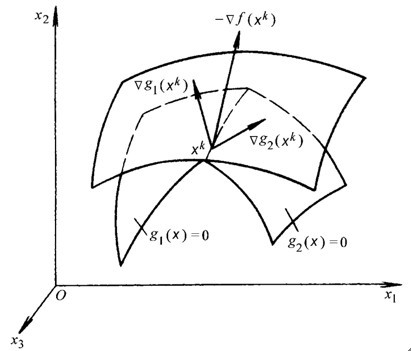
\includegraphics[width=0.5\textwidth]{KKT-geometry-1.jpg}
\end{FigureCenter}


注意我们上面推导过, 约束起作用时 $ g_{j}(\mathbf{x})=0 $, 所以此时约束在几何上应该是一簇\textbf{约束平面}.

我们假设在 $ \mathbf{x}^{*} $ 取得极小值点, 若同时满足 $ g_{1}(\mathbf{x})=0 $ 和 $ g_{2}(\mathbf{x})=0 $, 则 $ \mathbf{x}^{k} $ 一定在这两个平面的交线上, 且 $ -\nabla f\left(\mathbf{x}^{*}\right)=\sum_{j \in J} \mu_{j} \nabla g_{j}\left(\mathbf{x}^{*}\right) $, 即 $ -\nabla f\left(\mathbf{x}^{k}\right) 、 \nabla g_{1}\left(\mathbf{x}^{k}\right) $ 和 $ \nabla g_{2}\left(\mathbf{x}^{k}\right) $ 共面.

\begin{FigureCenter}{}
    \label{fig:kkt-2}
    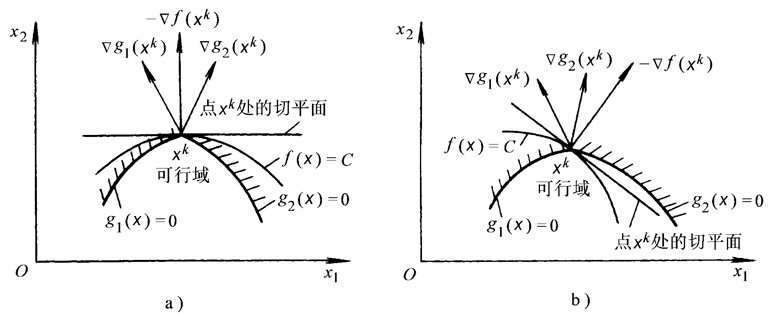
\includegraphics[width=\textwidth]{KKT-geometry-2.jpg}
\end{FigureCenter}

图\ref{fig:kkt-2}是在点 $ \mathbf{x}^{k} $ 处沿 $ x_{1} O x_{2} $ 面的截面, 过点 $ \mathbf{x}^{k} $ 作目标函数的负梯度 $ -\nabla f\left(\mathbf{x}^{k}\right) $, 它垂直于目标函数 的等值线 $ f(\mathbf{x})=C $ ,且指向目标函数 $ f(\mathbf{x}) $ 的最速减小方向.

\begin{corollary}
    一点的梯度与等值线相互垂直。
\end{corollary}

再作约束函数 $ g_{1}(\mathbf{x})=0 $ 和 $ g_{2}(\mathbf{x})=0 $ 的梯度 $ \nabla g_{1}\left(\mathbf{x}^{k}\right) $ 和 $ \nabla g_{2}\left(\mathbf{x}^{k}\right) $, 它们分别垂直 $ g_{1}(\mathbf{x})=0 $ 和 $ g_{2}(\mathbf{x})=0 $ 两曲面在 $ \mathbf{x}^{k} $ 的切平面, 并形成一个雉形夹角区域.此时, 可能有 $ \mathrm{a} 、 \mathrm{~b} $ 两种情形:

\begin{FigureCenter}{}
    \label{fig:kkt-3}
    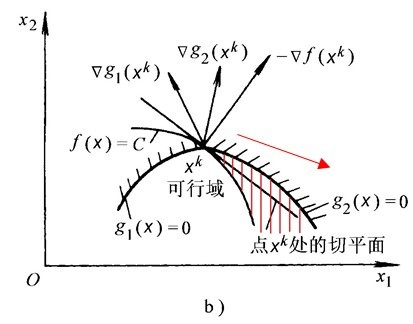
\includegraphics[width=0.5\textwidth]{KKT-geometry-3.jpg}
\end{FigureCenter}

我们先来看情形 $\mathrm{b}$ :若3个向量的位置关系如\ref{fig:kkt-3}所示, 即 $-\nabla f$ 落在 $\nabla g_{1}$ 和 $\nabla g_{2}$ 所形成的锥角区外的 一侧. 此时, 作等值面 $f(\mathbf{x})=C$ 在点 $\mathbf{x}^{k}$ 的切平面(它与 $-\nabla f\left(\mathbf{x}^{k}\right)$ 垂直), 我们发现:沿着与负 梯度 $-\nabla f$ 成锐角的方向移动(如下图红色箭头方向), 只要在红色区域取值, 目标函数 $f(\mathbf{x})$ 总 能减小.而红色区域是可行域 $(f(\mathbf{x})=C$, C取不同的常数能得到不同的等值线, 因此能取到红色 区域), 因此既可减小目标函数值, 又不破坏约束条件. 这说明 $\mathbf{x}^{k}$ 仍可沿约束曲面移动而不破坏约 束条件, 且目标函数值还能够减小.所以 $\mathbf{x}^{k}$ 不是稳定的最优点, 即不是局部极值点.

反过头来看情形a: $ -\nabla f $ 落在 $ \nabla g_{1} $ 和 $ \nabla g_{2} $ 形成的锥角内. 此时, 同样作 $ f(\mathbf{x})=C $ 在点 $ \mathbf{x}^{k} $ 与 $ -\nabla f $ 垂直的切平面. 当从 $ \mathbf{x}^{k} $ 出发沿着与负梯度 $ -\nabla f $ 成锐角的方向移动时, 虽然能使目标函数值减小, 但此时任何一点都不在可行区域内. 显然, 此时 $ \mathbf{x}^{k} $ 就是局部最优点 $ \mathbf{x}^{*} $, 再做任何移动都将破坏约 束条件, 故它是稳定点.

由于 $ -\nabla f\left(\mathbf{x}^{*}\right) $ 和 $ \nabla g_{1}\left(\mathbf{x}^{*}\right) 、 \nabla g_{2}\left(\mathbf{x}^{*}\right) $ 在一个平面内, 所以前者可看成是后两者的线性组合. 又由 上面的几何分析知, $ -\nabla f\left(\mathbf{x}^{*}\right) $ 在 $ \nabla g_{1}\left(\mathbf{x}^{*}\right) $ 和 $ \nabla g_{2}\left(\mathbf{x}^{*}\right) $ 的夹角之间, 所以线性组合的系数为正, 有
$$
-\nabla f\left(\mathbf{x}^{*}\right)=\mu_{1} \nabla g_{1}\left(\mathbf{x}^{*}\right)+\mu_{2} \nabla g_{2}\left(\mathbf{x}^{*}\right), \text { 且 } \mu_{1}>0, \mu_{2}>0 \text {. }
$$
这就是 $ \mu_{j}>0 $ 的原因. 类似地, 当有多个不等式约束同时起作用时, 要求 $ -\nabla f\left(\mathbf{x}^{*}\right) $ 处于 $ \nabla g_{j}\left(\mathbf{x}^{*}\right) $ 形成的超角锥(高维图形, 我姑且称之为 “超” )之内.

\subsection{总结:同时包含等式和不等式约束的一般优化问题}

\begin{theorem}[同时包含等式和不等式约束的一般优化问题的KKT条件]
    $$
\begin{array}{l}
\min f(\mathbf{x}) \\
\text { s.t. } g_{j}(\mathbf{x}) \leq 0(j=1,2, \cdots, m) \\
h_{k}(\mathbf{x})=0(k=1,2, \cdots, l)
\end{array}
$$
KKT条件 $ \left(\mathrm{x}^{*}\right. $ 是最优解的必要条件 $ ) $ 为
$$
\left\{\begin{array}{l}
\frac{\partial f}{\partial x_{i}}+\sum_{j=1}^{m} \mu_{j} \frac{\partial g_{j}}{\partial x_{i}}+\sum_{k=1}^{l} \lambda_{k} \frac{\partial h_{k}}{\partial x_{i}}=0,(i=1,2, \ldots, n) \\
h_{k}(\mathbf{x})=0,(k=1,2, \cdots, l) \\
\mu_{j} g_{j}(\mathbf{x})=0,(j=1,2, \cdots, m) \\
\mu_{j} \geq 0
\end{array}\right.
$$
\end{theorem}

\begin{remark}
    对于等式约束的Lagrange乘子,并没有非负的要求。
\end{remark}

\begin{remark}
    以后求其极值点,不必再引入松弛变量,直接使用KKT条件判断。
\end{remark}


\section[Supplement Material: 凸优化、拉格朗日乘子法和KKT条件]{Supplement Material: 凸优化、拉格朗日乘子法和KKT条件\footnote{Cited from \url{https://zhuanlan.zhihu.com/p/59928816}.}}

\subsection{凸集的概念}

\begin{definition}[点、(直)线、线段]
    $ x_{1} \neq x_{2} $ 是 $ \mathbb{R}^{n} $ 中的两\term{点}, $ \theta \in \mathbb{R} $, 那么 $ y=x_{2}+\theta\left(x_{1}-x_{2}\right) $ 表示穿过两点的\term{线}。

    当 $ 0 \leqslant \theta \leqslant 1 $ 时, $ y $ 是 $ x_{1} $ 到 $ x_{2} $ 的\term{线段},$ y $ 也可以表示成 $ y=\theta x_{1}+(1-\theta) x_{2} $。
\end{definition}

\begin{definition}[仿射集]
    一个集合 $ C \subseteq \mathbb{R}^{n} $ 是\term{仿射集}如果其中任意两个不同的点的连线仍包含于 $ C $ 。
\end{definition}

\begin{definition}[凸集]
    一个集合 $ C \subseteq \mathbb{R}^{n} $ 是凸集, 如果任意两点之间的线段仍包含于 $ C $ 。即 $ \forall x_{1}, x_{2} \in C $, 任意 $ 0 \leqslant \theta \leqslant 1 $, 有 $ \theta x_{1}+(1-\theta) x_{2} \in C $ 。
\end{definition}

\begin{theorem}
    两个凸集的交集仍是凸集。
\end{theorem}

\begin{definition}[凸函数]
    一个函数 $ f: \mathbb{R}^{n} \rightarrow \mathbb{R} $ 是\term{凸函数}如果定义域是凸集而且对任意定义域的 $ x, y, 0 \leqslant \theta \leqslant 1 $ 有
$$
f(\theta x+(1-\theta) y) \leqslant \theta f(x)+(1-\theta) f(y)
$$
\end{definition}

二维时候的几何意义是, 如果两点的线段总位于函数曲线之上, 那么该函数是凸函数。

\begin{theorem}
    $ f $ 是凸的, 那么 $ -f $ 是 凹的。
\end{theorem}

\begin{theorem}
    
仿射函数既凸又凹。
\end{theorem}


\begin{theorem}[$ \alpha- $sublevel 集]
    给定凸函数 $ f$,则$\{x \in D(f): f(x) \leqslant \alpha\} $是一个凸集。
\end{theorem}

\begin{proof}
    对任意 $ x, y \in D(f) $ 使得 $$ f(x) \leqslant \alpha, f(y) \leqslant \alpha $$
    
    有 $$ f(\theta x+(1-\theta) y) \leqslant \theta f(x)+(1-\theta) f(y) \leqslant \theta \alpha+(1-\theta) \alpha $$
    
    也就是说如果 $ x, y $ 属于 $ \alpha- $ sublevel 集,那么二者之间的线段上的点也可以使得 $ f \leqslant \alpha , $ 即二者之间的线段也包含于 $ \alpha- $ sublevel 集。
\end{proof}

\subsection{凸优化}

\begin{definition}[优化问题]
    \term{优化问题}有如下形式:

    $$
\begin{array}{ll}
\operatorname{minimize} & f_{0}(x) \\
\text { subject to } & f_{i}(x) \leqslant b_{i}, i=1, \ldots, m
\end{array}
$$

$ x=\left(x_{1}, \ldots, x_{n}\right) $ 是\term{优化变量}, 函数 $ f_{0}: \mathbb{R}^{n} \rightarrow \mathbb{R} $ 是\term{目标函数}, 函数 $ f_{i}: \mathbb{R}^{n} \rightarrow \mathbb{R} $ 是\term{约束函数}。 $ b_{i} $ 是约束。使得 $ f_{0}(x) $ 在约束条件下最小的 $ x^{*} $ 叫做\term{最优点}, 或问题的\term{解}。
\end{definition}

\begin{definition}[凸优化]
    \term{凸优化}问题有如下形式:

    $$
    \begin{array}{ll}
    \operatorname{minimize} & f(x) \\
    \text { subject to } & x \in C
    \end{array}
    $$
    
    $ f $ 是凸函数, $ C $ 是凸集。
\end{definition}

\begin{corollary}
    凸集可以表示成某些凸集的交集。
\end{corollary}

所以凸优化问题一般表示为

\begin{definition}[凸优化问题]
    \label{def:convex-problem}

    $$
    \begin{array}{ll}
    \operatorname{minimize} & f(x) \\
    \text { subject to } & g_{i}(x) \leqslant 0, i=1, \ldots, m \\
    & h_{j}(x)=0, j=1, \ldots, p
    \end{array}
    $$

    其中 $ g_{i} $ 是\term{凸函数}, $ h_{j} $ 是\term{仿射函数}。 
\end{definition}

$ g_{i}(x) \leqslant 0 $叫做 \term{$ 0- $sublevel集}, 是凸集。

\begin{theorem}
    $ h_{j}(x)=0 $ 也是凸集。
\end{theorem}

\begin{proof}
    $$ h\left(\theta x_{1}+(1-\theta) x_{2}\right)=\theta h\left(x_{1}\right)+(1-\theta) h\left(x_{2}\right)=0 $$
\end{proof}

凸优化问题的特点是, \textbf{所有局部最优点都是全局最优点}。

\begin{definition}[二次规划]
    如果一个凸优化问题的 $ g_{i} $ 都是仿射函数, 且 $ f $ 是凸二次函数, 那么它叫做二次规划:
    $$
    \begin{array}{ll}
    \operatorname{minimize} & \frac{1}{2} x^{\top} P x+c^{\top} x+d \\
    \text { subject to } & g_{i}(x) \leqslant 0, i=1, \ldots, m \\
    & h_{j}(x)=0, j=1, \ldots, p
    \end{array}
    $$

    其中 $ P $ 是一个对称半正定矩阵(使得 $ \left.\frac{1}{2} x^{\top} P x \geqslant 0\right) $ 。
\end{definition}



\subsection{拉格朗日对偶性}

\begin{theorem}
    对于没有限制的凸函数, 最优点 $ x^{*} $ 一定满足 $ \nabla_{x} f\left(x^{*}\right)=0 $。
\end{theorem}

然而对于有限制条件的凸优化问题却不是这样。拉格朗日对偶性可以将有限制的凸优化问题转化为没有限制的问题, 来求解凸优化问题。

\begin{definition}[拉格朗日函数]
    给定一个凸优化问题, 拉格朗日算子是一个函数 $ \mathcal{L}: \mathbb{R}^{n} \times \mathbb{R}^{m} \times \mathbb{R}^{p} \rightarrow \mathbb{R} $, 定义为:
    $$
    \mathcal{L}(x, \alpha, \beta)=f(x)+\sum_{i=1}^{m} \alpha_{i} g_{i}(x)+\sum_{i=1}^{p} \beta_{i} h_{i}(x)
    $$

    $ x \in \mathbb{R}^{n} $ 叫做\term{主变量(primal variable)}。 $ \alpha \in \mathbb{R}^{m}, \beta \in \mathbb{R}^{p} $ 统称对偶变量或拉格朗日乘子。
\end{definition}

\begin{theorem}
    总存在一个拉格朗日乘子, 使得没有限制的拉格朗日算子相对于 $ x $ 的最小值, 等于原凸优化问题的最优值
\end{theorem}

后文会证明。

\subsubsection{主问题}

为了说明拉格朗日算子和原凸优化问题的关系,需要引入主问题和对偶问题。

考虑优化问题:

\begin{problem}
    \label{pbl:primal}
    $$
\min _{x}\left[\max _{\alpha, \beta, \alpha_{i} \geqslant 0} \mathcal{L}(x, \alpha, \beta)\right]=\min _{x} \theta_{\mathcal{P}}(x)
$$

括号内的 $ \theta_{\mathcal{P}}: \mathbb{R}^{n} \rightarrow \mathbb{R} $ 叫做\term{主目标(primal objective)}, 等号右边的没有限制的最小化问题叫做\term{主问题(primal problem)}。 用 $ x^{*} $ 表示\term{主问题的解},$ p^{*}=\theta_{\mathcal{P}}\left(x^{*}\right) $ 表示\term{主目标的最优值}。
\end{problem}

\begin{definition}[primal feasible]
    $ x $ 是\term{主可行的(primal feasible)}如果 $ g_{i}(x) \leqslant 0, h_{j}(x)=0 $ 。
\end{definition}


$$
\begin{aligned}
\theta_{\mathcal{P}}(x) &=\max _{\alpha, \beta, \alpha_{i} \geqslant 0} \mathcal{L}(x, \alpha, \beta) \\
&=\max _{\alpha, \beta, \alpha_{i} \geqslant 0}\left[f(x)+\sum_{i=1}^{m} \alpha_{i} g_{i}(x)+\sum_{i=1}^{p} \beta_{i} h_{i}(x)\right] \\
&=f(x)+\max _{\alpha, \beta, \alpha_{i} \geqslant 0}\left[\sum_{i=1}^{m} \alpha_{i} g_{i}(x)+\sum_{i=1}^{p} \beta_{i} h_{i}(x)\right]
\end{aligned}
$$

观察最后一个式子:

\begin{itemize}
    \item 如果任何一个 $ g_{i}(x)>0 $, 那么最大化 $ \theta_{\mathcal{P}}(x) $ 只需要将相应的 $ \alpha_{i} $ 设置为无限大。
    \item 如果 $ g_{i}(x) \leqslant 0 $, 因为 $ \alpha_{i} \geqslant 0 $, 所以 $ \theta_{\mathcal{P}}(x) $ 最大时, 必然有 $ \alpha_{i}=0 $ 。
\end{itemize}

相似地:

\begin{itemize}
    \item 如果 $ h_{i} \neq 0 $, 那么最大化 $ \theta_{\mathcal{P}}(x) $ 只需要将相应的 $ \beta_{i} $ 设置为 $ h_{i}(x) $ 的相同符号且绝对值无限大。
    \item 如果 $ h_{i}(x)=0 $, 那么 $ \sum_{i=1}^{p} \beta_{i} h_{i}(x) $ 项的最大值为0 。
\end{itemize}

综上, 有
$$
\theta_{\mathcal{P}}(x)=\left\{\begin{array}{ll}
f(x)+0 & x \text { 为主可行的 } \\
f(x)+\infty & x \text { 不是主可行的 }
\end{array}\right.
$$
因此当 $ x $ 主可行时, 主问题\ref{pbl:primal}的最优值等于原凸优化问题\ref{def:convex-problem}的最优值。

\subsubsection{对偶问题}

\begin{definition}[对偶问题]
    对调主问题的最大最小操作:
$$
\max _{\alpha, \beta, \alpha \geqslant 0}\left[\min _{x} \mathcal{L}(x, \alpha, \beta)\right]=\max _{\alpha, \beta, \alpha \geqslant 0} \theta_{\mathcal{D}}(\alpha, \beta)
$$

$ \theta_{\mathcal{D}}(\alpha, \beta): \mathbb{R}^{m} \times \mathbb{R}^{p} \rightarrow \mathbb{R} $ 是\term{对偶目标(dual objective)},等号右边的有限制的最大化问题叫做\term{对偶问题}。 用 $ \left(\alpha^{*}, \beta^{*}\right) $ 表示\term{对偶问题的解}, $ d^{*}=\theta_{\mathcal{D}}\left(\alpha^{*}, \beta^{*}\right) $ 表示\term{对偶目标的最优值}。
\end{definition}

\begin{definition}[对偶可行]
    如果 $ \alpha_{i}(x) \geqslant 0 $ ,$ (\alpha, \beta) $ 是对偶可行的。
\end{definition}


\begin{theorem}
    如果 $ (\alpha, \beta) $ 是对偶可行的,那么 $ \theta_{\mathcal{D}}(\alpha, \beta) \leqslant p^{*} $.
\end{theorem}

\begin{proof}
    $$ \begin{aligned} \theta_{\mathcal{D}}(\alpha, \beta) &=\min _{x} \mathcal{L}(x, \alpha, \beta) \\ & \leqslant \mathcal{L}\left(x^{*}, \alpha, \beta\right) \\ &=f\left(x^{*}\right)+\sum_{i=1}^{m} \alpha_{i} g_{i}\left(x^{*}\right)+\sum_{i=1}^{p} \beta_{i} h_{i}\left(x^{*}\right) \\ & \leqslant f\left(x^{*}\right)=p^{*} \end{aligned} $$
\end{proof}

\begin{theorem}[弱对偶性]
    对任意主问题和对偶问题,有 $ d^{*} \leqslant p^{*} $.
\end{theorem}

\begin{theorem}[强对偶性]
    对任意主问题和对偶问题, 如果满足某个条件(constraint qualifications), 那 么 $ d^{*}=p^{*} $ 。最常用的constraint qualification是Slater's condition: 所有的不等式限制都严格满 足 (即 $ g_{i}(x)<0 $ ) 。
\end{theorem}

\begin{theorem}[Slater 条件]
    设定义在 $ \mathcal{D} $ 上的函数 $ f_{i}(\cdot), i=1,2, \cdots, n $ 为凸函数, $ g_{j}(\cdot), j=1,2, \cdots, m $ 为 仿射函数, 考虑凸优化问题

    $$
    \min _{\mathbf{x}} f_{0}(\mathbf{x}), \quad \text { s.t. } f_{i}(\mathbf{x}) \leq 0, g_{i}(\mathbf{x}) \leq 0
    $$

    如果存在点 $ \mathrm{x} \in $ relint $ \mathcal{D} $ (即 $ \mathcal{D} $ 的相对内点), 则强对偶性成立.
\end{theorem}

实践中, 几乎所有的凸优化问题都满足某种constraint qualification, 所以 主问题和对偶问题有相同的最优值。

\begin{theorem}[互补松弛性 (complementary slackness, KKT complementarity)]
    如果强对偶性满足, 那么 $ \alpha_{i}^{*} g\left(x_{i}^{*}\right)=0, i=1, \ldots, m $
    
\end{theorem}

\begin{proof}
    $$
    \begin{aligned}
    p^{*}=d^{*}=\theta_{\mathcal{D}}\left(\alpha^{*}, \beta^{*}\right) &=\min _{x} \mathcal{L}\left(x, \alpha^{*}, \beta^{*}\right) \\
    & \leqslant \mathcal{L}\left(x^{*}, \alpha^{*}, \beta^{*}\right) \\
    &=f\left(x^{*}\right)+\sum_{i=1}^{m} \alpha_{i}^{*} g_{i}\left(x^{*}\right)+\sum_{i=1}^{p} \beta_{i}^{*} h_{i}\left(x^{*}\right) \\
    & \leqslant f\left(x^{*}\right)=p^{*}
    \end{aligned}
    $$

    因为第一个和最后一个表达式相等, 所以中间所有的小于等于号都是等号, 有 $$ \sum_{i=1}^{m} \alpha_{i}^{*} g_{i}\left(x^{*}\right)+\sum_{i=1}^{p} \beta_{i}^{*} h_{i}\left(x^{*}\right)=0 $$

    因为 $ \alpha_{i}^{*} \geqslant 0 , h_{i}\left(x^{*}\right)=0 $, 所以 $ \alpha_{i}^{*} $ 和 $ g_{i}\left(x^{*}\right) $ 至少有一个是 0 。
\end{proof}

\begin{theorem}
    设 $ x^{*} \in \mathbb{R}^{n}, \alpha^{*} \in \mathbb{R}^{m}, \beta^{*} \in \mathbb{R}^{p} $, 下列条件为 $ \mathrm{KKT} $ 条件:

    \begin{enumerate}
        \item (主可行) $ g_{i}\left(x^{*}\right) \leqslant 0, i=1, \ldots, m, h_{j}\left(x^{*}\right)=0, j=1, \ldots, p $
        \item (对偶可行) $ \alpha_{i}^{*} \geqslant 0, i=1, \ldots, m $
        \item (互补松弛性) $ \alpha_{i}^{*} g\left(x_{i}^{*}\right)=0, i=1, \ldots, m $
        \item (Lagrangian Stationary) $ \nabla_{x} \mathcal{L}\left(x^{*}, \alpha^{*}, \beta^{*}\right)=0 $
    \end{enumerate}

\end{theorem}

\begin{theorem}
    对于凸优化问题, 有:

$ x^{*} $ 原始最优, $ \left(\alpha^{*}, \beta^{*}\right) $ 对偶最优,且有$$ 强对偶性 \Leftrightarrow  满足  K K T  条件$$
\end{theorem}

\subsection{总结}


给定一个\term{凸优化}问题, \term{拉格朗日算子}将凸优化问题的目标函数和限制考虑进一个函数中, 在拉格朗日算子基础上可以定义\term{主问题}和\term{对偶问题}。

\term{主问题}是先调整 $ (\alpha, \beta) $ 使拉格朗日算子最大(变为主目标), 再调整 $ x $ 使主目标最小。 $ x $ 主可行时, 主目标等于原凸优化问题的目标函数, 主目标的最小值等于原凸优化问题的最小值。

\term{对偶问题}是先调整 $ x $ 使拉格朗日算子最小(变为对偶目标, 因为拉格朗日算子是关于 $ x $ 的没有限制 的凸函数, 所以变为对偶目标时其对 $ x $ 的偏导数为 0 ), 再调整使对偶目标最大。 $ (\alpha, \beta) $ 对偶可行 时, 对偶目标小于等于主目标的最小值。

\term{弱对偶性}指对偶目标的最大值小于等于主目标的最小值。强对偶性指对偶目标的最大值等于主目标的最小值。

$$对偶目标的最大值=主目标的最小值=原凸优化问题的最小值 \Leftrightarrow^{当且仅当}满足KKT条件$$

因此,当对偶问题比原凸优化问题容易求解时,可以通过求解对偶问题来解原凸优化问题。


\section[Supplementary Material: KKT Conditions, Linear Programming and Nonlinear Programming]{Supplementary Material: KKT Conditions, Linear Programming and Nonlinear Programming \footnote{Written by Christopher Griffine. (\href{http://www.personal.psu.edu/cxg286/LinearProgramming.html}{Linear Programming})}}



\subsection{Karush-Kuhn-Tucker Theorem(s)}

\begin{theorem} Let $z : \mathbb{R}^n \rightarrow \mathbb{R}$ be a differentiable objective function, $g_i:\mathbb{R}^n \rightarrow \mathbb{R}$ be differentiable constraint functions for $i = 1,\dots,m$ and $h_j:\mathbb{R}^n \rightarrow \mathbb{R}$ be differentiable constraint functions for $j=1,\dots,l$. If $\mathbf{x}^* \in \mathbb{R}^n$ is an optimal point satisfying an appropriate regularity condition for the following optimization problem:

\begin{displaymath}
P\left\{
\begin{aligned}
\max\;\;& z(x_1,\dots,x_n)\\
s.t.\;\;& g_1(x_1,\dots,x_n) \leq 0\\
& \hspace*{0.5in}\vdots\\
& g_m(x_1,\dots,x_n) \leq 0\\
& h_1(x_1,\dots,x_n) = 0\\
&\hspace*{0.5in}\vdots\\
&h_l(x_1,\dots,x_n) = 0
\end{aligned}
\right.
\end{displaymath}

then there exists $\lambda_1,\dots,\lambda_m \in \mathbb{R}$ and $\mu_1,\dots\mu_l \in \mathbb{R}$ so that:

\begin{gather*}
\text{Primal Feasibility}: \left\{
\begin{aligned}
g_i(\mathbf{x}^*) \leq 0 \quad \text{for $i = 1,\dots,m$}\\
h_j(\mathbf{x}^*) = 0 \quad \text{for $j = 1,\dots,l$}
\end{aligned}
\right.\\
\text{Dual Feasibility}:\left\{
\begin{aligned}
\nabla z(\mathbf{x}^*) - \sum_{i = 1}^m\lambda_i\nabla g_i(\mathbf{x}^*) - \sum_{j = 1}^{l}\mu_j\nabla h_j(\mathbf{x}^*) = \mathbf{0}\\
\lambda_i \geq 0 \quad \text{for $i=1,\dots,m$}\\
\mu_j \in \mathbb{R} \quad \text{for $j = 1,\dots,l$}
\end{aligned}
\right.\\
\text{Complementary Slackness}:\left\{
\begin{aligned}
\lambda_ig_i(\mathbf{x}^*) = 0 \quad \text{for $i = 1,\dots,m$}
\end{aligned}
\right.
\end{gather*}
\label{thm:KKT7}
\end{theorem}

\begin{theorem} Let $z : \mathbb{R}^n \rightarrow \mathbb{R}$ be a differentiable concave  function, $g_i:\mathbb{R}^n \rightarrow \mathbb{R}$ be differentiable convex functions for $i = 1,\dots,m$ and $h_j:\mathbb{R}^n \rightarrow \mathbb{R}$ be affine functions for $j=1,\dots,l$. Suppose there are $\lambda_1,\dots,\lambda_m \in \mathbb{R}$ and $\mu_1,\dots\mu_l \in \mathbb{R}$ so that:

\begin{gather*}
\text{Primal Feasibility}: \left\{
\begin{aligned}
g_i(\mathbf{x}^*) \leq 0 \quad \text{for $i = 1,\dots,m$}\\
h_j(\mathbf{x}^*) = 0 \quad \text{for $j = 1,\dots,l$}
\end{aligned}
\right.\\
\text{Dual Feasibility}:\left\{
\begin{aligned}
\nabla z(\mathbf{x}^*) - \sum_{i = 1}^m\lambda_i\nabla g_i(\mathbf{x}^*) - \sum_{j = 1}^{l}\mu_j\nabla h_j(\mathbf{x}^*) = \mathbf{0}\\
\lambda_i \geq 0 \quad \text{for $i=1,\dots,m$}\\
\mu_j \in \mathbb{R} \quad \text{for $j = 1,\dots,l$}
\end{aligned}
\right.\\
\text{Complementary Slackness}:\left\{
\begin{aligned}
\lambda_ig_i(\mathbf{x}^*) = 0 \quad \text{for $i = 1,\dots,m$}
\end{aligned}
\right.
\end{gather*}

then $\mathbf{x}^*$ is a global maximizer for 
\begin{displaymath}
P\left\{
\begin{aligned}
\max\;\;& z(x_1,\dots,x_n)\\
s.t.\;\;& g_1(x_1,\dots,x_n) \leq 0\\
& \hspace*{0.5in}\vdots\\
& g_m(x_1,\dots,x_n) \leq 0\\
& h_1(x_1,\dots,x_n) = 0\\
&\hspace*{0.5in}\vdots\\
&h_l(x_1,\dots,x_n) = 0
\end{aligned}
\right.
\end{displaymath}
\label{thm:KKT8}
\end{theorem}

The values $\lambda_1,\dots,\lambda_m$ and $\mu_1,\dots,\mu_l$ are sometimes called \textit{Lagrange multipliers} and sometimes called \textit{dual variables}. Primal Feasibility, Dual Feasibility and Complementary Slackness are called the \textit{Karush-Kuhn-Tucker} (KKT) conditions.

\begin{remark} The regularity condition mentioned in Theorem \ref{thm:KKT7} is sometimes called a \term{constraint qualification}. A common one is that the gradients of the binding constraints are all linearly independent at $\mathbf{x}^*$. There are many variations of constraint qualifications. We will not deal with these in these notes. 
    
    Suffice it to say, all the problems we consider will automatically satisfy a constraint qualification, meaning the KKT theorem holds.
\end{remark}

\begin{remark} Theorem \ref{thm:KKT7} holds as a necessary condition even if $z(\mathbf{x})$ is not concave or the functions $g_i(\mathbf{x})$ ($i=1,\dots,m$) are not convex or the functions $h_j(\mathbf{x})$ ($j=1,\dots,l$) are not linear. In this case though, the fact that a triple: $(\mathbf{x},\boldsymbol{\lambda}, \boldsymbol{\mu}) \in \mathbb{R}^{n} \times \mathbb{R}^m \times \mathbb{R}^l$ does not ensure that this is an optimal solution for Problem $P$.
\end{remark}

Looking more closely at the dual feasibility conditions, we see something interesting. Suppose that there are \textit{no} equality constraints (i.e., not constraints of the form $h_j(\mathbf{x}) = 0$). Then the statements:

\begin{displaymath}
\begin{aligned}
\nabla z(\mathbf{x}^*) - \sum_{i = 1}^m\lambda_i \nabla g_i(\mathbf{x}^*) - \sum_{j = 1}^{l}\mu_j \nabla h_j(\mathbf{x}^*) & = \mathbf{0}\\
\lambda_i &\geq 0 \quad \text{for $i=1,\dots,m$}
\end{aligned}
\end{displaymath}

imply that:

\begin{displaymath}
\begin{aligned}
\nabla z(\mathbf{x}^*) &= \sum_{i = 1}^m\lambda_i \nabla g_i(\mathbf{x}^*)\\
\lambda_i &\geq 0 \quad \text{for $i=1,\dots,m$}
\end{aligned}
\end{displaymath}

Specifically, this says that the \textit{gradient of $z$ at $\mathbf{x}^*$ is a positive combination of the gradients of the constraints at $\mathbf{x}^*$.} But more importantly, since we also have \textit{complementary slackness}, we know that if $\mathbf{g}_i(\mathbf{x}^*) \neq 0$, then $\lambda_i = 0$ because $\lambda_i g_i(\mathbf{x}^*) = 0$ for $i = 1,\dots,m$. Thus, what dual feasibility is really saying is that \textit{gradient of $z$ at $\mathbf{x}^*$ is a positive combination of the  gradients of the \textbf{binding} constraints at $\mathbf{x}^*$.} Remember, a constraint is binding if $g_i(\mathbf{x}^*) = 0$, in which case $\lambda_i \geq 0$.


\begin{remark} Continuing from the previous remark, in the general case when we have some equality constraints, then dual feasibility says:
\begin{displaymath}
\begin{aligned}
\nabla z(\mathbf{x}^*) &= \sum_{i = 1}^m\lambda_i \nabla g_i(\mathbf{x}^*) + \sum_{j = 1}^{l}\mu_j \nabla h_j(\mathbf{x}^*)\\
\lambda_i &\geq 0 \quad \text{for $i=1,\dots,m$}\\
\mu_j &\in \mathbb{R}\quad \text{for $j=1,\dots,l$}
\end{aligned}
\end{displaymath}
Since equality constraints are \textit{always binding} this says that the \textit{gradient of $z$ at $\mathbf{x}^*$ is a linear combination of the  gradients of the \textbf{binding} constraints at $\mathbf{x}^*$.} 
\end{remark}

\subsection{Linear Programming and KKT Conditions - An Example}
Consider the following linear programming problem:
\begin{equation}
P \left \{
\begin{aligned}
\max \;\; & x_1 + x_2  \\ 
s.t. & x_1 + 2x_2 \leq 4\\
& 2x_1 + x_2 \leq 6\\
& x_1, x_2 \geq 0
\end{aligned} \right.
\end{equation}
Assuming I didn't know how to solve this problem using the Simplex method, I could look at Theorem \ref{thm:KKT8} and remark that the constraints and objective are all concave (and convex) since they are linear. Therefore, it suffices to find a KKT point and this point must be optimal.
We can re-write Problem $P$ in the form of Theorem \ref{thm:KKT7} as:
\begin{displaymath}
P \left \{
\begin{aligned}
\max \;\; & z(x_1,x_2) \equiv x_1 + x_2  \\ 
s.t. & g_1(x_1,x_2) \equiv x_1 + 2x_2 -4 \leq 0\\
& g_2(x_1,x_2) \equiv 2x_1 + x_2 - 6\leq 0\\
& g_3(x_1,x_2) \equiv -x_1 \leq 0\\
& g_4(x_1,x_2) \equiv -x_2 \leq 0
\end{aligned} \right.
\end{displaymath}

To write the KKT conditions, observe the following:
\begin{displaymath}
\nabla z = \begin{bmatrix}1\\1\end{bmatrix} \quad \quad \nabla g_1 = \begin{bmatrix}1\\2\end{bmatrix}
\quad\quad \nabla g_2 = \begin{bmatrix}2\\1\end{bmatrix} \quad \quad 
\nabla g_3 = \begin{bmatrix}-1\\0\end{bmatrix} \quad \quad \nabla g_4 = \begin{bmatrix}0\\-1\end{bmatrix}
\end{displaymath}
We can now write the KKT conditions for this problem as:
\begin{gather*}
\text{Primal Feasibility}: \left\{
\begin{aligned}
x_1 + 2x_2 &\leq 4\\
2x_1 + x_2 &\leq 6\\
x_1, x_2 &\geq 0
\end{aligned}
\right.\\
\text{Dual Feasibility}:\left\{
\begin{aligned}
\begin{bmatrix}1\\1\end{bmatrix} - \lambda_1\begin{bmatrix}1\\2\end{bmatrix} - 
\lambda_2\begin{bmatrix}2\\1\end{bmatrix} -\lambda_3\begin{bmatrix}-1\\0\end{bmatrix} - 
\lambda_4\begin{bmatrix}0\\-1\end{bmatrix} &= \begin{bmatrix}0\\0\end{bmatrix}\\
\lambda_1,\lambda_2,\lambda_3,\lambda_4 & \geq 0
\end{aligned}
\right.\\
\text{Complementary Slackness}:\left\{
\begin{aligned}
\lambda_1(x_1 + 2x_2 -4) &= 0\\
\lambda_2(2x_1 + x_2 - 6) &= 0\\
\lambda_3(-x_1) &= 0\\
\lambda_4(-x_2) &= 0
\end{aligned}
\right.
\end{gather*}
Consider Dual Feasibility for a moment. I can expand the matrices to obtain a system of equations:
\begin{displaymath}
\begin{aligned}
1 - \lambda_1 - 2\lambda_2 + \lambda_3 & = 0\\
1 - 2\lambda_1 - \lambda_2 + \lambda_4 & = 0\\
\lambda_1,\lambda_2,\lambda_3,\lambda_4 & \geq 0
\end{aligned}
\end{displaymath}
Or:
\begin{displaymath}
\begin{aligned}
\lambda_1 + 2\lambda_2 - \lambda_3 &= 1\\
2\lambda_1 + \lambda_2 - \lambda_4 &= 1\\
\lambda_1,\lambda_2,\lambda_3,\lambda_4 & \geq 0
\end{aligned}
\end{displaymath}
Since $\lambda_3, \lambda_4 \geq 0$, they act like \textit{surplus variables} and we can write the Dual Feasibility as:
\begin{equation}
\left\{
\begin{aligned}
\lambda_1 + 2\lambda_2 &\geq  1\\
2\lambda_1 + \lambda_2 &\geq 1\\
\lambda_1,\lambda_2& \geq 0
\end{aligned}\right.
\label{eqn:Lambda}
\end{equation}
\begin{remark} It would now suffice to find values for $x_1$, $x_2$, $\lambda_1$, $\lambda_2$, $\lambda_3$, and $\lambda_4$ the satisfy the KKT conditions and we could solve the linear programming problem $P$.
\end{remark}

We can show that the optimal point for this problem is $x = \tfrac{8}{3}$ and $y = \tfrac{2}{3}$ using a graphical method. Figure \ref{fig:KKTLP-1} shows the feasible region of the problem as well as the level curves of the objective function (curves for which $x_1 + x_2 = k$, where $k$ is a fixed constant). The value $k$ increases going left to right and bottom to top, so the optimal solution must occur at the intersection of the lines $x_1 + 2 x_2 = 4$ and $2x_1 + x_2 = 6$. You can compare the value of the objective at the proposed optimal point $x = \tfrac{8}{3}$ and $y = \tfrac{2}{3}$ to the value of the objective at the other extreme points. For example, at the extreme point $x = 3$, $y = 0$, we see the value of the objective is only $3$, as compared to $\tfrac{10}{3}$ at the point of optimality.


\begin{FigureCenter}{The feasible region for the example linear programming problem illustrating level curves of the objective.}
    \label{fig:KKTLP-1}
    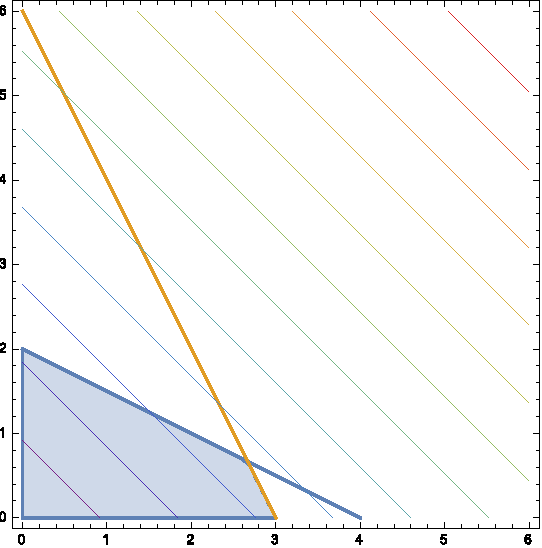
\includegraphics[width=0.4\textwidth]{imported_figures/KKTLP-1-eps-converted-to.pdf}
\end{FigureCenter}

\begin{FigureCenter}{The gradients of the objective function and the binding constraints at optimality and their geometric relation are illustrated}
    \label{fig:KKTLP-2}
    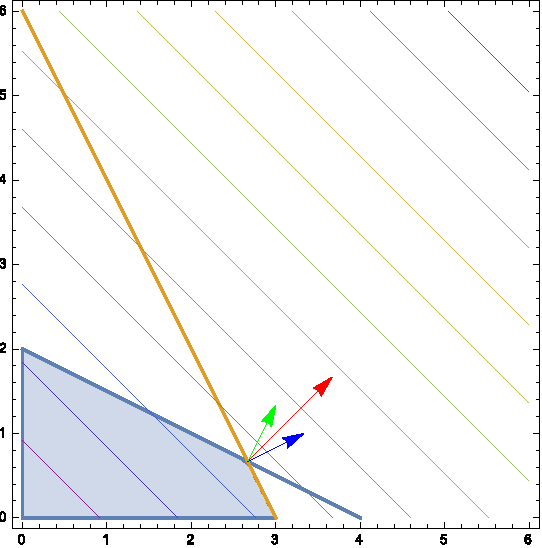
\includegraphics[width=0.4\textwidth]{imported_figures/KKTLP-2-eps-converted-to.pdf}
\end{FigureCenter}


We can now see that for the KKT conditions to hold, we must have $\lambda_3 = \lambda_4 = 0$ because $x_1 > 0$ and $x_2 > 0$ at optimality and complementary slackness requires that: $\lambda_3(-x_1) = 0$ and $\lambda_4(-x_2) = 0$ at optimality. This leaves $\lambda_1$ and $\lambda_2$. We know these must satisfy the equations in Expression \ref{eqn:Lambda}. Therefore, we see that when $\lambda_1 = \lambda_2 = \tfrac{1}{3}$, Expression 2 is satisfied. Thus: we have written:
\begin{equation}
\begin{bmatrix}1\\1\end{bmatrix} = \frac{1}{3}\begin{bmatrix}1\\2\end{bmatrix} - 
\frac{1}{3}\begin{bmatrix}2\\1\end{bmatrix}
\end{equation}
That is, we have expressed the gradient of the objective function ($\nabla z$) as a positive combination of the gradients of the \textit{binding} constraints ($\nabla g_1$ and $\nabla g_2$). This is shown in Figure \ref{fig:KKTLP-2}, in which we see the gradient of the objective function (red) inside the (cone of) the gradients of the binding constraints (blue and green).

\subsection{The Dual KKT Conditions}
Recall that if we are given a linear programming problem of the form:
\begin{equation}
P\left\{
\begin{aligned}
\max\;\; & \mathbf{c}^T\mathbf{x}\\
s.t.\;\; & \mathbf{A}\mathbf{x} \leq \mathbf{b}\\
& \mathbf{x} \geq 0
\end{aligned}\right.
\end{equation}

Then the dual problem for Problem $P$ is:
\begin{equation}
D\left\{
\begin{aligned}
\min\;\; & \mathbf{w}\mathbf{b}\\
s.t.\;\; & \mathbf{w}\mathbf{A} \geq \mathbf{c}^T\\
& \mathbf{w} \geq \mathbf{0}
\end{aligned}\right.
\end{equation}
Here we assume that $\mathbf{w}$ is a \textit{row} vector (unlike our usual assumption that all vectors are column vectors). In our example problem, we have:
\begin{displaymath}
\mathbf{A} = \begin{bmatrix}1 & 2\\2 & 1\end{bmatrix} \quad \quad \mathbf{c} = \begin{bmatrix}1\\1\end{bmatrix} \quad \quad \mathbf{b} = \begin{bmatrix}4\\6\end{bmatrix}
\end{displaymath}
Let us write:
\begin{displaymath}
\mathbf{w} = \begin{bmatrix} \lambda_1 & \lambda_2 \end{bmatrix}
\end{displaymath}
Then we can write the dual problem as:
\begin{displaymath}
D\left\{
\begin{aligned}
\min \;\; & \begin{bmatrix} \lambda_1 & \lambda_2 \end{bmatrix} \begin{bmatrix}4\\6\end{bmatrix} \\
& \begin{bmatrix} \lambda_1 & \lambda_2 \end{bmatrix} \begin{bmatrix}1 & 2\\2 & 1\end{bmatrix} \geq \begin{bmatrix}1 & 1\end{bmatrix}\\
& \lambda_1, \lambda_2 \geq 0
\end{aligned}
\right.
\end{displaymath}
This can be rewritten more concretely as:
\begin{displaymath}
D\left\{
\begin{aligned}
\min \;\; & 4\lambda_1 + 6\lambda_2\\
&\lambda_1 + 2\lambda_2 \geq 1\\
&2\lambda_1 + \lambda_2 \geq 1\\
& \lambda_1, \lambda_2 \geq 0
\end{aligned}
\right.
\end{displaymath}
Immediately we see a connection. The constraints of this problem look just like the simplified dual feasibility constraints. In fact, if we add surplus variables $\lambda_3, \lambda_4 \geq 0$, we see they match exactly and the problem in standard form is:
\begin{displaymath}
D\left\{
\begin{aligned}
\min \;\; & 4\lambda_1 + 6\lambda_2\\
&\lambda_1 + 2\lambda_2 - \lambda_3 = 1\\
&2\lambda_1 + \lambda_2 -\lambda_4 =1\\
& \lambda_1, \lambda_2,\lambda_3, \lambda_4 \geq 0
\end{aligned}
\right.
\end{displaymath}
We can complete our exploration of the relationship between these two problems by constructing the KKT conditions for the dual problem. First, re-write the dual as:
\begin{displaymath}
\begin{aligned}
\max\;\; & -4\lambda_1 - 6\lambda_2 \\
s.t. & -\lambda_1 - 2\lambda_2 + 1\leq 0\\
& -2\lambda_1 - \lambda_2 + 1\leq 0\\
& -\lambda_1 \leq 0\\
& -\lambda_2 \leq 0
\end{aligned}
\end{displaymath}
As before, we can write down the KKT conditions:
\begin{gather*}
\text{Primal Feasibility}: \left\{
\begin{aligned}
\lambda_1 + 2\lambda_2 &\geq 1\\
2\lambda_1 + \lambda_2 &\geq 1\\
\lambda_1, \lambda_2 & \geq 1
\end{aligned}
\right.\\
\text{Dual Feasibility}:\left\{
\begin{aligned}
\begin{bmatrix}-4\\-6\end{bmatrix} - x_1\begin{bmatrix}-1\\-2\end{bmatrix} - 
x_2\begin{bmatrix}-2\\-1\end{bmatrix} -s_1\begin{bmatrix}-1\\0\end{bmatrix} - 
s_2\begin{bmatrix}0\\-1\end{bmatrix} &= \begin{bmatrix}0\\0\end{bmatrix}\\
x_1,x_2,s_1,s_2 & \geq 0
\end{aligned}
\right.\\
\text{Complementary Slackness}:\left\{
\begin{aligned}
x_1(-\lambda_1 - 2\lambda_2 + 1) &= 0\\
x_2(-2\lambda_1 - \lambda_2 + 1) &= 0\\
s_1(-\lambda_1) &= 0\\
s_2(-\lambda_2) &= 0
\end{aligned}
\right.
\end{gather*}
Again, we can re-write the dual feasibility conditions (for which we have intentionally chosen specific dual variable names) and see they become:
\begin{displaymath}
\begin{aligned}
x_1 + 2x_2 + s_1 &= 4\\
2x_1 + x_2 + s_2 & =6\\
x_1,x_2, s_1, s_2 &\geq 0
\end{aligned}
\end{displaymath}
Since $s_1, s_2 \geq 0$, they act like \textit{slack variables} and thus we have:
\begin{displaymath}
\begin{aligned}
x_1 + 2x_2 &\leq  4\\
2x_1 + x_2 &\leq 6\\
x_1,x_2&\geq 0
\end{aligned}
\end{displaymath}
and we've recovered the constraints from the original primal problem as the dual feasibility conditions of the KKT conditions for the dual optimization problem. We can go further. Note:
\begin{align*}
-s_1 &= x_1 + 2x_2 - 4= -g_1(x_1,x_2)\\
-s_2 &= 2x_1 + x_2 -6 = -g_2(x_1,x_2)
\end{align*}
while from our earlier observations about the surplus variables $\lambda_3$ and $\lambda_4$ we know:
\begin{align*}
\lambda_3 &= -\lambda_1 - 2\lambda_2 + 1\\
-\lambda_4 &= -2\lambda_1 - \lambda_2 + 1
\end{align*}
Thus, complementary slackness from the primal problem is:
\begin{align*}
\lambda_3(-x_1) &= 0 \iff \lambda_3(x_1) =0  \iff 
	x_1(\lambda_1 + 2\lambda_2 - 1) = 0\\
\lambda_4(-x_2) &= 0 \iff \lambda_4(x_2) =0 \iff x_2(-2\lambda_1 - \lambda_2 + 1) = 0
\end{align*}
Likewise:
\begin{align*}
\lambda_1(x_1 + 2x_2 - 4) &=0 \iff \lambda_1(-s_1) = 0 \iff s_1(-\lambda_1) = 0\\
\lambda_2(2x_1 + x_2 - 6) &=0 \iff \lambda_2(-s_2) = 0 \iff s_2(-\lambda_2) = 0
\end{align*}
Thus, the complementary slackness conditions of the primal problem are identical to the complementary slackness conditions of the dual problem. This fact is true for linear programming problems in general.

\begin{remark} For an arbitrary linear programming problem and its dual, the KKT conditions for the primal and dual problems are \textbf{equivalent}, but the dual feasibility conditions for the primal problem are identical to the primal feasibility conditions for the dual problem and vice-versa. \textit{Thus, two linear programming problems are dual to each other if and only if they share KKT conditions with the primal and dual feasibility conditions swapped.}
\end{remark}

\begin{remark} We will use these results on KKT conditions and linear programs to discuss the solution (i.e., Nash equilibria) of zero-sum games via linear programming. We will then generalize these results to derive a quadratic programming problem whose optimal solutions will yield Nash equilibria. 
\end{remark}

\subsection{An Example from Nonlinear Programming}
Let's recall a simple optimization problem from differential calculus (Math 140): Goats are an environmentally friendly and inexpensive way to control a lawn when there are lots of rocks or lots of hills. (Seriously, both Google and some U.S. Navy bases use goats on rocky hills instead of paying lawn mowers!) 

Suppose I wish to build a pen to keep some goats. I have 100 meters of fencing and I wish to build the pen in a rectangle with the largest possible area. How long should the sides of the rectangle be? In this case, making the pen \textit{better} means making it have the largest possible area.

The problem is illustrated in Figure \ref{fig:GoatPen}.
\begin{figure}[htbp]
\centering
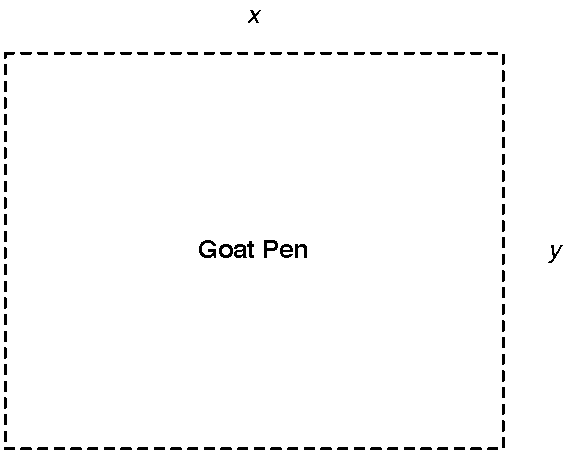
\includegraphics[scale=0.6]{imported_figures/GoatPen.pdf}
\caption{Goat pen with unknown side lengths. The objective is to identify the values of $x$ and $y$ that maximize the area of the pen (and thus the number of goats that can be kept).}
\label{fig:GoatPen}
\end{figure}
Clearly, we know that:
\begin{equation}
2x + 2y = 100
\label{eqn:GoatPerimeter}
\end{equation}
because $2x + 2y$ is the perimeter of the pen and I have 100 meters of fencing to build my pen. The area of the pen is $A(x,y) = xy$. We can use Equation \ref{eqn:GoatPerimeter} to solve for $x$ in terms of $y$. Thus we have:
\begin{equation}
y = 50 - x
\end{equation}
and $A(x) = x(50-x)$. To maximize $A(x)$, recall we take the first derivative of $A(x)$ with respect to $x$, set this derivative to zero and solve for $x$:
\begin{equation}
\frac{dA}{dx} = 50-2x = 0;
\end{equation}
Thus, $x = 25$ and $y = 50-x = 25$. We further recall from basic calculus how to confirm that this is a maximum; note:
\begin{equation}
\left.\frac{d^2A}{dx^2}\right|_{x = 25} = -2 < 0
\end{equation}
Which implies that $x = 25$ is a \textit{local maximum} for this function. Another way of seeing this is to note that $A(x) = 50x-x^2$ is an concave (a frowning parabola). As we could have guessed, a square will maximize the area available for holding goats. 

We can re-write the problem to be in a more common form
\begin{equation}
\left\{
\begin{aligned}
\max \;\; & A(x,y) = x y \\
s.t. \;\; & 2x + 2y = 100 \equiv 2x + 2y - 100 = 0\\
& x \geq 0 \equiv -x \leq 0\\
& y \geq 0 \equiv -y \leq 0 
\end{aligned}\right.
\label{eqn:GoatMax}
\end{equation}
Note we've added two inequality constraints $x \geq 0$ and $y \geq 0$ because it doesn't really make any sense to have negative lengths. In our problem, we now have: $g_1(x,y) = -x$ and $g_2(x,y) = -y$ and $h(x,y) = 2x+2y-100$ to be consistent with the notation in Theorem \ref{thm:KKT7}. It is worth noting, we could have used the constraint $2x + 2y - 100 \leq 0$ instead and obtained the same answer.

For the point of optimality ($x=25$, $y=25$), let us now compute the KKT conditions. Note first:
\begin{displaymath}
\nabla A = \begin{bmatrix}y\\x\end{bmatrix} \quad \quad 
\nabla h = \begin{bmatrix}2\\2\end{bmatrix} \quad \quad 
\nabla g_1 = \begin{bmatrix}-1\\0\end{bmatrix} \quad \quad 
\nabla g_2 = \begin{bmatrix}0\\-1\end{bmatrix} \quad \quad 
\end{displaymath}
Substituting $x^* = y^* = 25$, we can see that primal feasibility is obviously satisfied. Moreover:
\begin{displaymath}
\nabla A(x^*,y^*) = \begin{bmatrix}25\\25\end{bmatrix}
\end{displaymath}
We  consider only dual feasibility and complimentary slackness. 
\begin{gather*}
\text{Dual Feasibility}:\left\{
\begin{aligned}
\begin{bmatrix}25\\25\end{bmatrix} -\lambda_1\begin{bmatrix}-1\\0\end{bmatrix} - 
\lambda_2\begin{bmatrix}0\\-1\end{bmatrix} - \mu\begin{bmatrix}2\\2\end{bmatrix} &= \begin{bmatrix}0\\0\end{bmatrix}\\
\lambda_1,\lambda_2 & \geq 0\\
\mu &\in \mathbb{R}
\end{aligned}
\right.\\
\text{Complementary Slackness}:\left\{
\begin{aligned}
\lambda_1(-x^*) = \lambda_1\cdot(-25) &= 0\\
\lambda_2(-y^*) = \lambda_2\cdot(-25) &= 0
\end{aligned}
\right.
\end{gather*}
Notice we substituted $x^*$ and $y^*$ into the complementary slackness equations. From complementary slackness, we see at once that $\lambda_1 = \lambda_2 = 0$. This means dual feasibility reduces to:
\begin{displaymath}
\begin{bmatrix}25\\25\end{bmatrix} - \mu\begin{bmatrix}2\\2\end{bmatrix} = \begin{bmatrix}0\\0\end{bmatrix}
\end{displaymath}
The solution: $\mu = 25/2$ satisfies this equality. Notice the gradient of the objective and the gradient of the (single) binding constraint are parallel. Notice also unlike a linear programming problem, the optimal solution to this problem \textit{does not} occur at the extreme point of the constraint set (which is really just the line segment $2x + 2y = 100$ with $x,y\geq 0$). This geometric interpretation is illustrated in Figure \ref{fig:KKTNLP}. The gradient of the objective is shown in red, the gradient of the binding constraint is shown in green. Note, the gradient of the binding constraint has been scaled for visual effect. As expected, the level curves shown are given by the (implicit) equation $xy = k$. As you go up and right, the value of $k$ increases.
\begin{figure}[htbp]
\centering
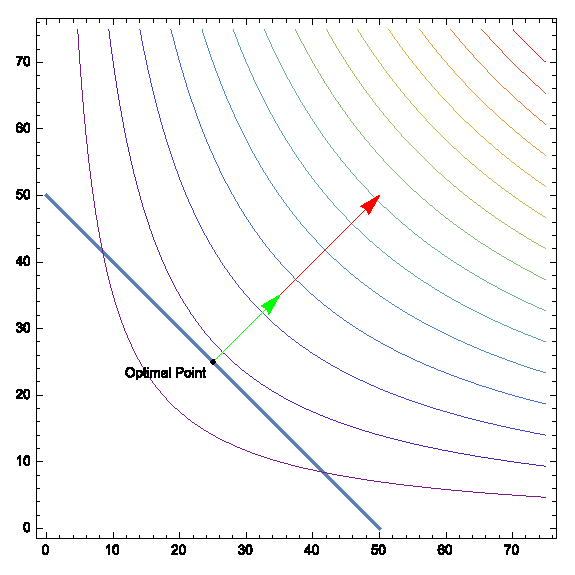
\includegraphics[scale=0.75]{imported_figures/KKTNLP.eps}
\caption{Visualization of the KKT conditions for a simple nonlinear programming problem. Notice the point of optimality is not at an extreme point. Moreover, the gradient of the binding constraint is parallel to the gradient of the objective, as expected. \textit{Note, the gradient of the binding constraint has been scaled larger for visual effect.}}
\label{fig:KKTNLP}
\end{figure}

\section[Supplementary Material: KKT Conditions ]{Supplementary Material: KKT Conditions \footnote{These notes are taken from \href{https://www.stat.cmu.edu/~ryantibs/convexopt/}{Machine Learning 10-725 (Convex Optimization)}.}}


\subsection{Dual Problem}

Given the following convex minimization problem:

\begin{problem}[convex minimization problem]
    \label{pro:kkt-problem}
    $$
\begin{array}{ll}
\min _{x} & f(x) \\
\text { subject to } & h_{i}(x) \leq 0, \quad i=1, \ldots, m \\
& \ell_{j}(x)=0, \quad j=1, \ldots, r
\end{array}
$$
The Lagrangian is defined as $ L(x, u, v)=f(x)+\sum_{u=1}^{m} u_{i} h_{i}(x)+\sum_{j=1}^{r} v_{j} \ell_{j}(x) . $ The Lagrange dual function is defined as $ g(u, v)=\min _{x} L(x, u, v) $. The dual problem is
$$
\begin{array}{ll}
\max _{u, v} & g(u, v) \\
\text { subject to } & u \geq 0
\end{array}
$$
\end{problem}


The Lagrange dual function $ g(u, v) $ is always \term{concave} regardless of whether the primal problem is convex or not.

\term{Weak duality}: $ f^{*} \geq g^{*} $ holds for all problems, where $ f^{*} $ and $ g^{*} $ are primal and dual optimal values, respectively.

Slaters's condition, which says the primal has at least one strictly feasible point, is a sufficient condition for \term{strong duality} to hold. If $ \exists x $ such that $ h_{i}(x)<0, i=1, \ldots, m $ and $ \ell_{j}(x)=0, j=1, \ldots, r, f^{*}=g^{*} $. This condition can be further refined to $ h_{i}(x)<0 $ for all $ i $ such that $ h_{i} $ is nonaffine. As a result, Slater's condition is reduced to feasibility for LP's.

\section{Karush-Kuhn-Tucker (KKT) Conditions}

For the given problem \ref{pro:kkt-problem}, the KKT conditions are:

\begin{enumerate}
    \item $ 0 \in \partial_{x}\left(f(x)+\sum_{i=1}^{m} u_{i} h_{i}(x)+\sum_{j=1}^{r} v_{j} \ell_{j}(x)\right) $ (stationary)
    \item $ u_{i} \cdot h_{i}(x)=0 $ for all $ i $ (complementary slackness)
    \item $ h_{i}(x) \leq 0, \ell_{j}(x)=0 $ for all $ i, j $ (primal feasibility)
    \item $ u_{i} \geq 0 $ for all $ i $ (dual feasibility)
\end{enumerate}

\begin{theorem}
    \label{thm:kkt-sufficient}
    For $ x^{*} $ and $ u^{*}, v^{*} $ to be primal and dual solutions, KKT conditions are sufficient.
\end{theorem}

\begin{proof}
    Proof: 
    
    Sufficiency: if $ \exists x^{*} $ and $ u^{*}, v^{*} $ that satisfy the KKT conditions, $ g\left(u^{*}, v^{*}\right)=f\left(x^{*}\right)+\sum_{i=1}^{m} u_{i}^{*} h_{i}\left(x^{*}\right)+ $ $ \sum_{j=1}^{r} v_{j}^{*} \ell_{j}\left(x^{*}\right)=f\left(x^{*}\right) $ 
    
    The first equality holds from stationarity, since $ f(x)+\sum_{i=1}^{m} u_{i} h_{i}(x)+\sum_{j=1}^{r} v_{j} \ell_{j}(x) $ is convex, so any stationary point is a minimizer, and the second holds by complementary slackness. 
    
    By weak duality, $ x^{*} $ and $ u^{*}, v^{*} $ are optimal. It always implies that the duality gap is 0 .
\end{proof}

\begin{theorem}
    For a problem with strong duality (e.g. assume Slater's condition: convex problem and there exists $ x $ strictly satisfying nonaffine inequality constraints),

    $ x^{*} $ and $ u^{*}, v^{*} $ are primal and dual solutions $ \Longleftrightarrow x^{*} $ and $ u^{*}, v^{*} $ satisfy the KKT conditions
\end{theorem}


\begin{proof}

    Sufficiency: Follows from Theorem \ref{thm:kkt-sufficient}.


    Necessity: Let $ x^{*} $ and $ u^{*}, v^{*} $ be primal and dual solutions, and suppose we know strong duality holds.Then

    $$
    \begin{aligned}
    f\left(x^{*}\right) &=g\left(u^{*}, v^{*}\right) \\
    &=\min _{x}\left(f(x)+\sum_{i=1}^{m} u_{i}^{*} h_{i}(x)+\sum_{j=1}^{r} v_{j}^{*} \ell_{j}(x)\right) \\
    & \leq f\left(x^{*}\right)+\sum_{i=1}^{m} u_{i}^{*} h_{i}\left(x^{*}\right)+\sum_{j=1}^{r} v_{j}^{*} \ell_{j}\left(x^{*}\right) \\
    & \leq f\left(x^{*}\right)
    \end{aligned}
    $$

The LSH equals RHS, so all inequalities in the equation must be equalities. Looking at the KKT conditions one by one, primal and dual feasibility holds, by virtue of optimality. Stationarity comes from the fact that $ x^{*} $ minimizes $ f(x)+\sum_{i=1}^{m} u_{i}^{*} h_{i}(x)+\sum_{j=1}^{r} v_{j}^{*} \ell_{j}(x) $. Since $ x^{*} $ is the minimizer, it must be a stationary point for this function. Complementary slackness comes from $ f\left(x^{*}\right)+\sum_{i=1}^{m} u_{i}^{*} h_{i}\left(x^{*}\right)+\sum_{j=1}^{r} v_{j}^{*} \ell_{j}\left(x^{*}\right)=f\left(x^{*}\right) $, since we must have $ \sum_{i=1}^{m} u_{i}^{*} h_{i}\left(x^{*}\right)=0 $ and they are each non-negative.

\end{proof}
\chapter{非线性最小二乘法}

\section{非线性最小二乘法的定义}

\begin{problem}
    $ f_{1}(x), \ldots, f_{m}(x) $ 是可微函数;

    优化目标: \begin{equation} \min _{x} \sum_{i=1}^{m}\left(f_{i}(x)\right)^{2} \end{equation}

\end{problem}

\begin{problem}
    \label{pbl:non-linear-least-squares}
    设函数 $ f(x): \mathfrak{R}^{n} \rightarrow \mathfrak{R}^{m} $ ,其第 $ i $ 个分量为函数 $ f_{i}(x)$

    则有
    \begin{equation}
    f(x)=\left[\begin{array}{c}
    f_{1}(x) \\
    f_{2}(x) \\
    \vdots \\
    f_{m}(x)
    \end{array}\right]
    \end{equation}

    优化目标
    \begin{equation} \min _{x} \sum_{i=1}^{m}\left(f_{i}(x)\right)^{2}=\|f(x)\|_{2}^{2} \end{equation}
\end{problem}


如果 $ f(x)=A x-b $ ,问题简化为(线性)最小二乘问题。

\subsection{例子:距离测量定位}

\begin{problem}
    向量 $ x_{e x} $ 表示二维或三维中的未知位置,通过测量到的已知点 $ a_{1}, \cdots, a_{m} $ 的距离来估计 $ x_{e x} $ 

    \begin{equation}
    \rho_{i}=\left\|x_{e x}-a_{i}\right\|_{2}+v_{i}, \quad i=1, \cdots, m
    \end{equation}

    其中 $ v_{i} $ 是测量误差。
\end{problem}

非线性最小二乘法估计:通过最小化估计 $ \hat{x} $的位置

\begin{equation}
\min _{x} \sum_{i=1}^{m}\left(\left\|x-a_{i}\right\|_{2}-\rho_{i}\right)^{2}=\|f(x)\|_{2}^{2}
\end{equation}

函数$ f_{i}(x)=\left\|x-a_{i}\right\|_{2}-\rho_{i} $ 是 $ f(x) $ 的 $ i $ 个分量。

% todo (2021-12-09 17:19): figure

\subsection{例子:多个相机视图定位}

\begin{remark}
    这个例子与遥感卫星成像等有关。
\end{remark}

建立一个理想的相机模型,由参数 $ A \in \mathfrak{R}^{2 \times 3}, b \in \mathfrak{R}^{2}, c \in \mathfrak{R}^{3}, d \in \mathfrak{R} $ 来描述。相机及其位置和方向用 $ A , b , c , d $ 来刻画。

目标位置 $ x \in \mathfrak{R}^{3} $ 在二维平面图像投影位置 $ x^{\prime} \in \mathfrak{R}^{2} $ .

\begin{equation}
x^{\prime}=\frac{1}{c^{T} x+d}(A x+b)
\end{equation}

如果物体在摄像机前面,则 $ c^{T} x+d>0 $ .

\begin{problem}
    位于 $ x_{e x} $ 位置的物体由 $ l $ 个相机观察(由 $ A_{i}, b_{i}, c_{i}, d_{i} $ 描述),目标在相机图像平面上位置 $ y_{i} \in \mathfrak{R}^{2} $

    \begin{equation}
    y_{i}=\frac{1}{c_{i}^{T} x_{e x}+d_{i}}\left(A_{i} x_{\alpha x}+b_{i}\right)+v_{i}
    \end{equation}

    $ v_{i} $ 为测量误差或量化误差。目的是从 $ l $ 个观测点 $ y_{1}, \ldots, y_{l} $ 来估计三维位置 $ x_{e x} $ .
\end{problem}


使用非线性最小二乘法估计
\begin{equation}
\min _{x} \sum_{i=1}^{l}\left\|\frac{1}{c_{i}^{T} x+d_{i}}\left(A_{i} x+b_{i}\right)-y_{i}\right\|_{2}^{2}
\end{equation}

这是关于 $ m=2 l $ 的非线性最小二乘法问题, $ \left(y_{i}\right)_{j} $ 是 $ y_{i} $ 的第 $ j $ 个 分量:
\begin{equation}
f_{i}(x)=\frac{\left(A_{i} x+b_{i}\right)_{1}}{c_{i}^{T} x+d_{i}}-\left(y_{i}\right)_{1}, \quad f_{l+i}(x)=\frac{\left(A_{i} x+b_{i}\right)_{2}}{c_{i}^{T} x+d_{i}}-\left(y_{i}\right)_{2}
\end{equation}

\subsection{例子:模型拟合}

\begin{problem}
\begin{equation}
\min _{\theta} \sum_{i=1}^{N}\left(\hat{f}\left(x^{(i)}, \theta\right)-y^{(i)}\right)^{2}
\end{equation}

$ \left(x^{(i)}, y^{(i)}\right), i=1, \cdots, N $ 表示样本。设函数 $ \hat{f}(x, \theta) $ 的参数 $ \theta = \left(\theta_{1}, \ldots, \theta_{p}\right) $.最小化的目标是估计函数参数 $ \theta $.
\end{problem}

假设函数 $ \hat{f}(x, \theta) $ 关于 $ \theta $ 的线性函数
\begin{equation}
\hat{f}(x, \theta)=\theta_{1} f_{1}(x)+\cdots+\theta_{p} f_{p}(x)
\end{equation}

当然 $ \hat{f}(x, \theta) $ 也可以是关于 $ \theta $ 的非线性函数。

\begin{example}
    有四个变量 $ \theta_{1}, \theta_{2}, \theta_{3}, \theta_{4} $ 的非线性最小二乘问题:
\begin{equation}
\min _{\theta} \sum_{i=1}^{N}\left(\theta_{1} e^{\theta_{2} x(i)} \cos \left(\theta_{3} x^{(i)}+\theta_{4}\right)-y^{(i)}\right)^{2}
\end{equation}

% todo (2021-12-09 19:15): figure
\end{example}

\subsection{例子:正交距离回归}

正交距离回归目标: 最小化 $ \hat{f}(x, \theta) $ 图中数据点到曲线的均方距离。 

例子: 三次多项式的正交距离回归:
\begin{equation}
\hat{f}(x, \theta)=\theta_{1}+\theta_{2} x+\theta_{3} x^{2}+\theta_{4} x^{3}
\end{equation}

% todo (2021-12-09 19:16): figure

\subsection{非线性最小二乘法}

\begin{problem}
    \begin{equation}
\min _{\theta, u^{(i)}} \sum_{i=1}^{N}\left(\left(\hat{f}\left(u^{(i)}, \theta\right)-y^{(i)}\right)^{2}+\left\|u^{(i)}-x^{(i)}\right\|_{2}^{2}\right)
\end{equation}

这个模型需要优化参数 $ \theta $ 和 $ {N} $ 个点 $ u^{(i)} $.
\end{problem}

第 $ i $ 项为数据点 $ \left(x^{(i)}, y^{(i)}\right) $ 到点 $ \left(u^{(i)}, \hat{f}\left(u^{(i)}, \theta\right)\right) $ 距离的平方。

\begin{FigureCenter}{优化模型的几何意义}
    

\tikzset{every picture/.style={line width=0.75pt}} %set default line width to 0.75pt        

\begin{tikzpicture}[x=0.75pt,y=0.75pt,yscale=-1,xscale=1]
%uncomment if require: \path (0,300); %set diagram left start at 0, and has height of 300

%Shape: Free Drawing [id:dp5002881259079404] 
\draw  [color={rgb, 255:red, 0; green, 0; blue, 0 }  ][line width=3] [line join = round][line cap = round] (63.01,245.57) .. controls (68.41,202.42) and (91.96,183.67) .. (133.01,168.57) .. controls (164.12,157.14) and (219.01,152.23) .. (219.01,106.57) ;
%Straight Lines [id:da19530315633268636] 
\draw [color={rgb, 255:red, 184; green, 84; blue, 80 }  ,draw opacity=1 ][line width=2.25]    (75.99,98.05) -- (139.99,166.05) ;
%Straight Lines [id:da6781226747978477] 
\draw [line width=1.5]  [dash pattern={on 5.63pt off 4.5pt}]  (75.99,98.05) -- (76.01,166.1) ;
%Straight Lines [id:da3955370838358767] 
\draw [line width=1.5]  [dash pattern={on 5.63pt off 4.5pt}]  (76.01,166.1) -- (139.99,166.05) ;
%Shape: Circle [id:dp03457846112388152] 
\draw  [color={rgb, 255:red, 245; green, 166; blue, 35 }  ,draw opacity=1 ][fill={rgb, 255:red, 245; green, 166; blue, 35 }  ,fill opacity=1 ] (135.98,166.05) .. controls (135.98,163.84) and (137.77,162.04) .. (139.99,162.04) .. controls (142.2,162.04) and (144,163.84) .. (144,166.05) .. controls (144,168.27) and (142.2,170.06) .. (139.99,170.06) .. controls (137.77,170.06) and (135.98,168.27) .. (135.98,166.05) -- cycle ;
%Shape: Circle [id:dp15280043442217006] 
\draw  [color={rgb, 255:red, 245; green, 166; blue, 35 }  ,draw opacity=1 ][fill={rgb, 255:red, 245; green, 166; blue, 35 }  ,fill opacity=1 ] (71.98,98.05) .. controls (71.98,95.84) and (73.77,94.04) .. (75.99,94.04) .. controls (78.2,94.04) and (80,95.84) .. (80,98.05) .. controls (80,100.27) and (78.2,102.06) .. (75.99,102.06) .. controls (73.77,102.06) and (71.98,100.27) .. (71.98,98.05) -- cycle ;

% Text Node
\draw (37,65.44) node [anchor=north west][inner sep=0.75pt]  [xscale=0.75,yscale=0.75]  {$\left( x^{( i)} ,y^{( i)}\right)$};
% Text Node
\draw (113,110.4) node [anchor=north west][inner sep=0.75pt]  [xscale=0.75,yscale=0.75]  {$d_{i}$};
% Text Node
\draw  [color={rgb, 255:red, 0; green, 0; blue, 0 }  ,draw opacity=0 ][fill={rgb, 255:red, 152; green, 195; blue, 245 }  ,fill opacity=1 ]  (256,117) .. controls (256,114.24) and (258.24,112) .. (261,112) -- (546,112) .. controls (548.76,112) and (551,114.24) .. (551,117) -- (551,151) .. controls (551,153.76) and (548.76,156) .. (546,156) -- (261,156) .. controls (258.24,156) and (256,153.76) .. (256,151) -- cycle  ;
\draw (259,116.4) node [anchor=north west][inner sep=0.75pt]  [xscale=0.75,yscale=0.75]  {$d_{i}^{2} =\left(\hat{f}\left( u^{(i)} ,\theta \right) -y^{(i)}\right)^{2} +\left\Vert u^{(i)} -x^{(i)}\right\Vert _{2}^{2}$};
% Text Node
\draw (131,174.4) node [anchor=north west][inner sep=0.75pt]  [xscale=0.75,yscale=0.75]  {$\left( u^{(i)} ,\hat{f}\left( u^{(i)} ,\theta \right)\right)$};


\end{tikzpicture}
\end{FigureCenter}

通过 $ u^{(i)} $ 与图中点 $ \left(x^{(i)}, y^{(i)}\right) $ 的平方距离来最小化 $ d_{i}^{2} $.最小化 $ \sum_{i} d_{i}^{2} $ ,即通过 $ u^{(1)}, \ldots, u^{(N)} $ 和 $ \theta $ 来最小化均方距离。

\subsection{二分类}

二分类的目标函数为 $ \hat{f}(x, \theta)=\operatorname{sign}\left(\theta_{1} f_{1}(x)+\theta_{2} f_{2}(x)+\cdots+\theta_{p} f_{p}(x)\right) $ 


\begin{problem}[二分类问题]
    \begin{equation}
\min _{\theta} \sum_{i=1}^{N}\left(\phi\left(\theta_{1} f_{1}\left(x^{(i)}\right)+\cdots+\theta_{p} f_{p}\left(x^{(i)}\right)\right)-y^{(i)}\right)^{2}
\end{equation}

$ \left(x^{(i)}, y^{(i)}\right) $ 是数据点, $ y^{(i)} \in\{-1,1\} $ . $ \phi(u) $ 是sigmoid函数,它是 $\operatorname{sign} (u) $ 函数的一个可微的近似函数。
\begin{equation}
\phi(u)=\frac{e^{u}-e^{-u}}{e^{u}+e^{-u}}
\end{equation}
\end{problem}


通过计算 $ \theta $ 来求解非线性最小二乘问题,\textbf{大概率}能得到良好的结果。



\section{梯度}

\subsection{Gradient and Directional Derivative}

\begin{definition}[$\mathfrak{R}^{n} \rightarrow \mathfrak{R}$函数$g$的梯度]
    可微函数 $ g: \mathfrak{R}^{n} \rightarrow \mathfrak{R} $ 在 $ z \in \mathfrak{R}^{n} $ 的梯度(gradient)为

\begin{equation}
\nabla g(z)=\left[\begin{array}{c}
\frac{\partial g}{\partial x_{1}}(z) \\
\frac{\partial g}{\partial x_{2}}(z) \\
\cdots \\
\frac{\partial g}{\partial x_{n}}(z)
\end{array}\right]
\end{equation}
\end{definition}

\begin{definition}[$g$在$z$附近的仿射近似(一阶泰勒公式,线性化)]
    \begin{equation} \begin{aligned} \hat{g}(x) &=g(z)+\frac{\partial g}{\partial x_{1}}(z)\left(x_{1}-z_{1}\right)+\cdots+\frac{\partial g}{\partial x_{n}}(z)\left(x_{n}-z_{n}\right) \\ &=g(z)+\nabla g(z)^{T}(x-z) \end{aligned} \end{equation}
\end{definition}

\begin{definition}[Directional Derivative]
    For given $ z $ and nonzero $ v $, define $ h(t)=g(z+t v) $

   The derivative of $ h $ at $ t=0 $
\begin{equation}
\begin{aligned}
h^{\prime}(0) &=\frac{\partial g}{\partial x_{1}}(z) v_{1}+\frac{\partial g}{\partial x_{2}}(z) v_{2}+\cdots+\frac{\partial g}{\partial x_{n}}(z) v_{n} \\
&=\nabla g(z)^{T} v
\end{aligned}
\end{equation}

This is called the \term{directional derivative} of $ g $ (at $ z $, in the direction $ v $ ), $ v $ is a \term{descent direction} of $ g $ at $ z $ if $ \nabla g(z)^{T} v<0 $.
\end{definition}

\subsection{Jacobian Matrices}


\begin{definition}[Jacobian Matrices]
    可微函数 $ f: \mathfrak{R}^{n} \rightarrow \mathfrak{R}^{m} $ 在 $ z \in \mathfrak{R}^{n} $ 的导数矩阵(Jacobian矩阵)

\begin{equation}
f(x)=\left[\begin{array}{c}
f_{1}(x) \\
f_{2}(x) \\
\vdots \\
f_{m}(x)
\end{array}\right] \quad D f(z)=\left[\begin{array}{cccc}
\frac{\partial f_{1}}{\partial x_{1}}(z) & \frac{\partial f_{1}}{\partial x_{2}}(z) & \cdots & \frac{\partial f_{1}}{\partial x_{n}}(z) \\
\frac{\partial f_{2}}{\partial x_{1}}(z) & \frac{\partial f_{2}}{\partial x_{2}}(z) & \cdots & \frac{\partial f_{2}}{\partial x_{n}}(z) \\
\vdots & \vdots & & \vdots \\
\frac{\partial f_{m}}{\partial x_{1}}(z) & \frac{\partial f_{m}}{\partial x_{2}}(z) & \cdots & \frac{\partial f_{m}}{\partial x_{n}}(z)
\end{array}\right]
\end{equation}
\end{definition}

\begin{definition}[$ f $ 在 $ z $ 附近的仿射近似(线性化)]
    \begin{equation}\begin{aligned}
        \hat{f} (x) & =f(z)+Df(z)(x-z)\\
         & =\left[\begin{array}{ c }
        f_{1} (z)\\
        f_{2} (z)\\
        \vdots \\
        f_{m} (z)
        \end{array}\right] \ +\left(\left[\begin{array}{ c c c c }
        \textcolor[rgb]{0.72,0.33,0.31}{\frac{\partial f_{1}}{\partial x_{1}} (z)} & \textcolor[rgb]{0.72,0.33,0.31}{\frac{\partial f_{1}}{\partial x_{2}} (z)} & \textcolor[rgb]{0.72,0.33,0.31}{\cdots } & \textcolor[rgb]{0.72,0.33,0.31}{\frac{\partial f_{1}}{\partial x_{n}} (z)}\\
        \frac{\partial f_{2}}{\partial x_{1}} (z) & \frac{\partial f_{2}}{\partial x_{2}} (z) & \cdots  & \frac{\partial f_{2}}{\partial x_{n}} (z)\\
        \vdots  & \vdots  &  & \vdots \\
        \frac{\partial f_{m}}{\partial x_{1}} (z) & \frac{\partial f_{m}}{\partial x_{2}} (z) & \cdots  & \frac{\partial f_{m}}{\partial x_{n}} (z)
        \end{array}\right]\left[\begin{array}{ c }
        \textcolor[rgb]{0.72,0.33,0.31}{x_{1} -z_{1}}\\
        \textcolor[rgb]{0.72,0.33,0.31}{x_{2} -z_{2}}\\
        \textcolor[rgb]{0.72,0.33,0.31}{\vdots }\\
        \textcolor[rgb]{0.72,0.33,0.31}{x_{n} -z_{n}}
        \end{array}\right]\right)_{m\times 1}
        \end{aligned}\end{equation}

    用符号 $ \hat{f}(x ; z) $ 表示点 $ z $ 附近的线性化逼近。
\end{definition}

\subsection{Hessian}

\begin{definition}[Hessian Matrices]
    Hessian of $ g $ at $ z $ is a symmetric $ n \times n $ matrix $ \nabla^{2} g(z) $ with elements
\begin{equation}
\nabla^{2} g(z)_{i j}=\frac{\partial^{2} g}{\partial x_{i} \partial x_{j}}(z)
\end{equation}

This is also the derivative matrix $ D f(z) $ of $ f(x)=\nabla g(x) $ at $ z $.
\end{definition}

\begin{definition}[Quadratic (second order) approximation of $g$ around $z$]
    \begin{equation} g_{{q}}(x)=g(z)+\nabla g(z)^{T}(x-z)+\frac{1}{2}(x-z)^{T} \nabla^{2} g(z)(x-z) \end{equation}
\end{definition}

\begin{example}
    Affine function: $ g(x)=a^{T} x+b $
\begin{equation}
\nabla g(x)=a, \quad \nabla^{2} g(x)=0
\end{equation}

Quadratic function: $ g(x)=x^{T} P x+q^{T} x+r $ with $ P $ symmetric
\begin{equation}
\nabla g(x)=2 P x+q, \quad \nabla^{2} g(x)=2 P
\end{equation}

Least squares cost: $ g(x)=\|A x-b\|^{2}=x^{T} A^{T} A x-2 b^{T} A x+b^{T} b $
\begin{equation}
\nabla g(x)=2 A^{T} A x-2 A^{T} b, \quad \nabla^{2} g(x)=2 A^{T} A
\end{equation}
\end{example}

\begin{theorem}[Linear combination properties]
    If $ g(x)=\alpha_{1} g_{1}(x)+\alpha_{2} g_{2}(x) $, then
\begin{equation}
\begin{aligned}
\nabla g(x) &=\alpha_{1} \nabla g_{1}(x)+\alpha_{2} \nabla g_{2}(x) \\
\nabla^{2} g(x) &=\alpha_{1} \nabla^{2} g_{1}(x)+\alpha_{2} \nabla^{2} g_{2}(x)
\end{aligned}
\end{equation}
\end{theorem}

\begin{theorem}[Composition with affine mapping properties]
    if $ g(x)=h(C x+d) $, then
\begin{equation}
\begin{aligned}
\nabla g(x) &=C^{T} \nabla h(C x+d) \\
\nabla^{2} g(x) &=C^{T} \nabla^{2} h(C x+d) C
\end{aligned}
\end{equation}
\end{theorem}

\begin{example}
    \begin{equation} g\left(x_{1}, x_{2}\right)=e^{x_{1}+x_{2}-1}+e^{x_{1}-x_{2}-1}+e^{-x_{1}-1} \end{equation}

    Gradient
\begin{equation}
\nabla g(x)=\left[\begin{array}{c}
e^{x_{1}+x_{2}-1}+e^{x_{1}-x_{2}-1}-e^{-x_{1}-1} \\
e^{x_{1}+x_{2}-1}-e^{x_{1}-x_{2}-1}
\end{array}\right]
\end{equation}

Hessian
\begin{equation}
\nabla^{2} g(x)=\left[\begin{array}{cc}
e^{x_{1}+x_{2}-1}+e^{x_{1}-x_{2}-1}+e^{-x_{1}-1} & e^{x_{1}+x_{2}-1}-e^{x_{1}-x_{2}-1} \\
e^{x_{1}+x_{2}-1}-e^{x_{1}-x_{2}-1} & e^{x_{1}+x_{2}-1}+e^{x_{1}-x_{2}-1}
\end{array}\right]
\end{equation}

Gradient and Hessian via composition property:

express $ g $ as $ g(x)=h(C x+d) $ with $ h\left(y_{1}, y_{2}, y_{3}\right)=e^{y_{1}}+e^{y_{2}}+e^{y_{3}} $ and
\begin{equation}
C=\left[\begin{array}{rr}
1 & 1 \\
1 & -1 \\
-1 & 0
\end{array}\right], \quad d=\left[\begin{array}{l}
-1 \\
-1 \\
-1
\end{array}\right]
\end{equation}

Gradient: $ \nabla g(x)=C^{T} \nabla h(C x+d) $
\begin{equation}
\nabla g(x)=\left[\begin{array}{rrr}
1 & 1 & -1 \\
1 & -1 & 0
\end{array}\right]\left[\begin{array}{c}
e^{x_{1}+x_{2}-1} \\
e^{x_{1}-x_{2}-1} \\
e^{-x_{1}-1}
\end{array}\right]
\end{equation}

Hessian: $ \nabla^{2} g(x)=C^{T} \nabla h^{2}(C x+d) C $
\begin{equation}
\nabla^{2} g(x)=\left[\begin{array}{rrr}
1 & 1 & -1 \\
1 & -1 & 0
\end{array}\right]\left[\begin{array}{ccc}
e^{x_{1}+x_{2}-1} & 0 & 0 \\
0 & e^{x_{1}-x_{2}-1} & 0 \\
0 & 0 & e^{-x_{1}-1}
\end{array}\right]\left[\begin{array}{rr}
1 & 1 \\
1 & -1 \\
-1 & 0
\end{array}\right]
\end{equation}
\end{example}

\subsection{Optimality conditions for twice differentiable $ g $}

\begin{theorem}[Necessary condition for twice differentiable $ g $]
    If $ x^{\star} $ is locally optimal, then
$ \nabla g\left(x^{\star}\right)=0 $ and $ \nabla^{2} g\left(x^{\star}\right) $ is positive semidefinite
\end{theorem}

\begin{theorem}[Sufficient condition]
    If $ x^{\star} $ satisfies
$ \nabla g\left(x^{\star}\right)=0 $ and $ \nabla^{2} g\left(x^{\star}\right) $ is positive definite
then $ x^{\star} $ is locally optimal.
\end{theorem}

\begin{definition}[Convex functions]
    $ g $ is called \textit{convex} if $ \nabla^{2} g(x) $ is positive semidefinite everywhere.
\end{definition}

\begin{theorem}[Necessary and sufficient condition for convex functions]
    if $ g $ is convex then $ x^{\star} $ is optimal if and only if $ \nabla g\left(x^{\star}\right)=0 $
\end{theorem}




\begin{example}
    $ g(x)=\log \left(e^{x}+e^{-x}\right) $
\begin{equation}
g^{\prime}(x)=\frac{e^{x}-e^{-x}}{e^{x}+e^{-x}}, \quad g^{\prime \prime}(x)=\frac{4}{\left(e^{x}+e^{-x}\right)^{2}}
\end{equation}
$ g^{\prime \prime}(x) \geq 0 $ everywhere; $ x^{\star}=0 $ is the unique optimal point
\end{example}

\begin{example}
    - $ g(x)=x^{4} $
\begin{equation}
g^{\prime}(x)=4 x^{3}, \quad g^{\prime \prime}(x)=12 x^{2}
\end{equation}
$ g^{\prime \prime}(x) \geq 0 $ everywhere; $ x^{\star}=0 $ is the unique optimal point
\end{example}

\begin{example}
    - $ g(x)=x^{3} $
\begin{equation}
g^{\prime}(x)=3 x^{2}, \quad g^{\prime \prime}(x)=6 x
\end{equation}
$ g^{\prime}(0)=0, g^{\prime \prime}(0)=0 $ but $ x=0 $ is not locally optimal
\end{example}

\begin{example}
    - $ g(x)=x^{T} P x+q^{T} x+r $ (P is symmetric positive definite)
\begin{equation}
\nabla g(x)=2 P x+q, \quad \nabla^{2} g(x)=2 P
\end{equation}
$ \nabla^{2} g(x) $ is positive definite everywhere, hence the unique optimal point is
\begin{equation}
x^{\star}=-(1 / 2) P^{-1} q
\end{equation}
\end{example}

\begin{example}
    - $ g(x)=\|A x-b\|^{2} $ ( $ A $ is a matrix with linearly independent columns)
\begin{equation}
\nabla g(x)=2 A^{T} A x-2 A^{T} b, \quad \nabla^{2} g(x)=2 A^{T} A
\end{equation}
$ \nabla^{2} g(x) $ is positive definite everywhere, hence the unique optimal point is
\begin{equation}
x^{\star}=\left(A^{T} A\right)^{-1} A^{T} b
\end{equation}
\end{example}

\begin{example}
    \begin{equation} g\left(x_{1}, x_{2}\right)=e^{x_{1}+x_{2}-1}+e^{x_{1}-x_{2}-1}+e^{-x_{1}-1} \end{equation}

    Gradient
\begin{equation}
\nabla g(x)=\left[\begin{array}{c}
e^{x_{1}+x_{2}-1}+e^{x_{1}-x_{2}-1}-e^{-x_{1}-1} \\
e^{x_{1}+x_{2}-1}-e^{x_{1}-x_{2}-1}
\end{array}\right]
\end{equation}

Hessian
\begin{equation}
\nabla^{2} g(x)=\left[\begin{array}{cc}
e^{x_{1}+x_{2}-1}+e^{x_{1}-x_{2}-1}+e^{-x_{1}-1} & e^{x_{1}+x_{2}-1}-e^{x_{1}-x_{2}-1} \\
e^{x_{1}+x_{2}-1}-e^{x_{1}-x_{2}-1} & e^{x_{1}+x_{2}-1}+e^{x_{1}-x_{2}-1}
\end{array}\right]
\end{equation}


    We can express $ \nabla^{2} g(x) $ as
\begin{equation}
\nabla^{2} g(x)=\left[\begin{array}{rrr}
1 & 1 & 1 \\
1 & -1 & 0
\end{array}\right]\left[\begin{array}{ccc}
e^{x_{1}+x_{2}-1} & 0 & 0 \\
0 & e^{x_{1}-x_{2}-1} & 0 \\
0 & 0 & e^{-x_{1}-1}
\end{array}\right]\left[\begin{array}{rr}
1 & 1 \\
1 & -1 \\
1 & 0
\end{array}\right]
\end{equation}
this shows that $ \nabla^{2} g(x) $ is positive definite for all $ x $
therefore $ x^{\star} $ is optimal if and only if
\begin{equation}
\nabla g\left(x^{\star}\right)=\left[\begin{array}{c}
e^{x_{1}^{\star}+x_{2}^{\star}-1}+e^{x_{1}^{\star}-x_{2}^{\star}-1}-e^{-x_{1}^{\star}-1} \\
e^{x_{1}^{\star}+x_{2}^{\star}-1}-e^{x_{1}^{\star}-x_{2}^{\star}-1}
\end{array}\right]=0
\end{equation}
two nonlinear equations in two variables
\end{example}


\section{求解非线性最小二乘法:目标梯度}

对于优化问题\ref{pbl:non-linear-least-squares}
\begin{equation} g(x)=\|f(x)\|_{2}^{2}=\sum_{i=1}^{m}\left(f_{i}(x)\right)^{2},f(x)=\left[\begin{array}{c}f_{1}(x) \\ f_{2}(x) \\ \vdots \\ f_{m}(x)\end{array}\right] \end{equation}

$ g $ 对 $ x_{j} $ 的一阶导数为
\begin{equation}\begin{aligned}
    \frac{\partial g}{\partial x_{j}} (z) & =2\sum _{i=1}^{m} f_{i} (z)\frac{\partial f_{i}}{\partial x_{j}} (z)\\
     & =2\left[\frac{\partial f_{\textcolor[rgb]{0.49,0.83,0.13}{1}}}{\partial x_{\textcolor[rgb]{0.29,0.56,0.89}{j}}} (z),\frac{\partial f_{\textcolor[rgb]{0.49,0.83,0.13}{2}}}{\partial x_{\textcolor[rgb]{0.29,0.56,0.89}{j}}} (z),\cdots ,\frac{\partial f_{\textcolor[rgb]{0.49,0.83,0.13}{m}}}{\partial x_{\textcolor[rgb]{0.29,0.56,0.89}{j}}} (z)\right]\left[\begin{array}{ c }
    f_{1} (z)\\
    f_{2} (z)\\
    \vdots \\
    f_{m} (z)
    \end{array}\right]
    \end{aligned}\end{equation}

注意到

\begin{equation}\displaystyle (Df(z))^{T} =\left[\begin{array}{ c c c c }
    \frac{\partial f_{\textcolor[rgb]{0.49,0.83,0.13}{1}}}{\partial x_{\textcolor[rgb]{0.29,0.56,0.89}{1}}} (z) & \frac{\partial f_{\textcolor[rgb]{0.49,0.83,0.13}{2}}}{\partial x_{\textcolor[rgb]{0.29,0.56,0.89}{1}}} (z) & \cdots  & \frac{\partial f_{\textcolor[rgb]{0.49,0.83,0.13}{m}}}{\partial x_{\textcolor[rgb]{0.29,0.56,0.89}{1}}} (z)\\
    \frac{\partial f_{\textcolor[rgb]{0.49,0.83,0.13}{1}}}{\partial x_{\textcolor[rgb]{0.29,0.56,0.89}{2}}} (z) & \frac{\partial f_{\textcolor[rgb]{0.49,0.83,0.13}{2}}}{\partial x_{\textcolor[rgb]{0.29,0.56,0.89}{2}}} (z) & \cdots  & \frac{\partial f_{\textcolor[rgb]{0.49,0.83,0.13}{m}}}{\partial x_{\textcolor[rgb]{0.29,0.56,0.89}{2}}} (z)\\
    \vdots  & \vdots  &  & \vdots \\
    \frac{\partial f_{\textcolor[rgb]{0.49,0.83,0.13}{1}}}{\partial x_{\textcolor[rgb]{0.29,0.56,0.89}{n}}} (z) & \frac{\partial f_{\textcolor[rgb]{0.49,0.83,0.13}{2}}}{\partial x_{\textcolor[rgb]{0.29,0.56,0.89}{n}}} (z) & \cdots  & \frac{\partial f_{\textcolor[rgb]{0.49,0.83,0.13}{m}}}{\partial x_{\textcolor[rgb]{0.29,0.56,0.89}{n}}} (z)
    \end{array}\right] =[ \nabla f_{1} (z),\nabla f_{2} (z),\cdots ,\nabla f_{m} (z)]\end{equation}

    $ g $ 在 $ z $ 的梯度为
    \begin{equation}
    \nabla g(z)=\left[\begin{array}{c}
    \frac{\partial g}{\partial x_{1}}(z) \\
    \vdots \\
    \frac{\partial g}{\partial x_{n}}(z)
    \end{array}\right]=2 \sum_{i=1}^{m} f_{i}(z) \nabla f_{i}(z)=2(D f(z))^{T} f(z)
    \end{equation}

\begin{theorem}[非线性最小二乘问题的最优必要条件]
        \begin{equation}
    \min _{x} g(x)=\sum_{i=1}^{m} f_{i}(x)^{2} \quad f(x)=\left[\begin{array}{c}
    f_{1}(x) \\
    f_{2}(x) \\
    \vdots \\
    f_{m}(x)
    \end{array}\right]
    \end{equation}

    如果要 $ x $ 使 $ g(x) $ 最小,则必须满足:
    \begin{equation}
    \nabla g(x)=2 D f(x)^{T} f(x)=0
    \end{equation}
\end{theorem}

\begin{corollary}[正规方程的最优必要条件]
    推广到正规方程,如果 $ f(x)=A x-b $ ,那么 $ D f(x)=A $ 和
\begin{equation}
\nabla g(x)=2 A^{T}(A x-b)
\end{equation}
\end{corollary}

\begin{remark}
    对于一般函数 $ f(x), \nabla g(x)=0 $ \textbf{不是最优解的充分条件}.
\end{remark}



\section{Gauss-Newton Algorithm}

\begin{problem}
    \begin{equation}
\min _{x} g(x)=\|f(x)\|_{2}^{2}=\sum_{i=1}^{m} f_{i}(x)^{2}
\end{equation}

从某个初始值 $ x^{(1)} $ 开始,当迭代 $ x^{(2)}, x^{(3)}, \ldots $.
\end{problem}

函数 $ f $ 在 $ x^{(k)} $ 附近的泰勒展开式是

\begin{equation}
\hat{f}\left(x ; x^{(k)}\right)=f\left(x^{(k)}\right)+D f\left(x^{(k)}\right)\left(x-x^{(k)}\right)
\end{equation}

用仿射近似 $ \hat{f}\left(x, x^{(k)}\right) $ 代替最小二乘法问题中函数 $ f(x) $

\begin{equation}
x^{(k+1)}=\arg \min _{x}\left\|\hat{f}\left(x ; x^{(k)}\right)\right\|_{2}^{2}
\end{equation}

第$k$次迭代问题:
\begin{equation}
\begin{array}{c}
x^{(k+1)}=\arg \min _{x}\left\|\hat{f}\left(x ; x^{(k)}\right)\right\|_{2}^{2} \\
x^{(k+1)}=\arg \min _{x} h(x)=\left\|f\left(x^{(k)}\right)+D f\left(x^{(k)}\right)\left(x-x^{(k)}\right)\right\|_{2}^{2}
\end{array}
\end{equation}

函数 $ h(x) $ 的梯度:
\begin{equation}
\nabla h(x)=2 D f\left(x^{(k)}\right)^{T}\left(f\left(x^{(k)}\right)+D f\left(x^{(k)}\right)\left(x-x^{(k)}\right)\right)=0
\end{equation}

则有
\begin{equation} D f\left(x^{(k)}\right)^{T} D f\left(x^{(k)}\right) x^{(k)}-D f\left(x^{(k)}\right)^{T} f\left(x^{(k)}\right)=D f\left(x^{(k)}\right)^{T} D f\left(x^{(k)}\right) x \end{equation}

\begin{equation} D f\left(x^{(k)}\right)^{T} D f\left(x^{(k)}\right) x^{(k)}-D f\left(x^{(k)}\right)^{T} f\left(x^{(k)}\right)=D f\left(x^{(k)}\right)^{T} D f\left(x^{(k)}\right) x \end{equation}

如果 $ D f\left(x^{(k)}\right) $ 的列是线性无关的,则其解为:
\begin{equation}
x^{(k+1)}=x^{(k)}-\left(D f\left(x^{(k)}\right)^{T} D f\left(x^{(k)}\right)\right)^{-1} D f\left(x^{(k)}\right)^{T} f\left(x^{(k)}\right)
\end{equation}

高斯-牛顿法步骤 $ \Delta x^{(k)}=x^{(k+1)}-x^{(k)} $ :
\begin{equation}
\begin{aligned}
\Delta x^{(k)} &=-\left(D f\left(x^{(k)}\right)^{T} D f\left(x^{(k)}\right)\right)^{-1} D f\left(x^{(k)}\right)^{T} f\left(x^{(k)}\right) \\
&=-\frac{1}{2}\left(D f\left(x^{(k)}\right)^{T} D f\left(x^{(k)}\right)\right)^{-1} \nabla g\left(x^{(k)}\right)
\end{aligned}
\end{equation}

(利用第14.10的 $ \nabla g(x) $ 表达式).

逼近函数 $ \hat{f}\left(x ; x^{(k)}\right) $ 的关于 $ x^{(k+1)} $ 的代价:
\begin{equation}
\begin{aligned}
\|\left.\hat{f}\left(x^{(k+1)} ; x^{(k)}\right)\right|_{2} ^{2} &=\| f\left(x^{(k)}\right)+D f\left(x^{(k)}\right) \Delta x^{(k)}||_{2}^{2} \\
&=\left\|\left.f\left(x^{(k)}\right)\right|_{2} ^{2}+2 f\left(x^{(k)}\right)^{T} D f\left(x^{(k)}\right) \Delta x^{(k)}+\right\| D f\left(x^{(k)}\right) \Delta x^{(k)} \|_{2}^{2}
\end{aligned}
\end{equation}

\begin{equation}\begin{aligned}
    & 2Df\left( x^{(k)}\right)^{T}\left( f\left( x^{(k)}\right) +Df\left( x^{(k)}\right)\left( x^{(k+1)} -x^{(k)}\right)\right) =0\quad ( 目标梯度等于0)\\
   \Rightarrow  & Df\left( x^{(k)}\right)^{T} f\left( x^{(k)}\right) =-Df\left( x^{(k)}\right)^{T} Df\left( x^{(k)}\right) \Delta x^{(k)}\\
   \Rightarrow  & \left( \Delta x^{(k)}\right)^{T} Df\left( x^{(k)}\right)^{T} f\left( x^{(k)}\right) =-\left( \Delta x^{(k)}\right)^{T} Df\left( x^{(k)}\right)^{T} Df\left( x^{(k)}\right) \Delta x^{(k)} =-\left\Vert Df\left( x^{(k)}\right) \Delta x^{(k)}\right\Vert _{2}^{2}
   \end{aligned}\end{equation}

\begin{equation} \left\|\hat{f}\left(x^{(k+1)} ; x^{(k)}\right)\right\|_{2}^{2}=\left\|f\left(x^{(k)}\right)\right\|_{2}^{2}-\left\|D f\left(x^{(k)}\right) \Delta x^{(k)}\right\|_{2}^{2} \end{equation}

如果 $ D f\left(x^{(k)}\right) $ 的列向量线性无关,且 $ \Delta x^{(k)} \neq 0 $ :

\begin{equation} \left\|D f\left(x^{(k)}\right) \Delta x^{(k)}\right\|_{2}^{2}>0 \Rightarrow\left\|\hat{f}\left(x^{(k+1)} ; x^{(k)}\right)\right\|_{2}^{2}<\left\|f\left(x^{(k)}\right)\right\|_{2}^{2} \end{equation}

当 $ {m}={n} $ 时, $ D f\left(x^{(k)}\right) $ 的列向量线性无关,高斯-牛顿法可简化为

\begin{equation}
\begin{aligned}
x^{(k+1)} &=x^{(k)}-\left(D f\left(x^{(k)}\right)^{T} D f\left(x^{(k)}\right)\right)^{-1} D f\left(x^{(k)}\right)^{T} f\left(x^{(k)}\right) \\
&=x^{(k)}-\left(D f\left(x^{(k)}\right)\right)^{-1}\left(D f\left(x^{(k)}\right)^{T}\right)^{-1} D f\left(x^{(k)}\right)^{T} f\left(x^{(k)}\right) \\
&=x^{(k)}-\left(D f\left(x^{(k)}\right)\right)^{-1} f\left(x^{(k)}\right) .
\end{aligned}
\end{equation}


如果 $ m=n=1 $ 时,迭代更新可进一步简化为

\begin{equation} x^{(k+1)}=x^{(k)}-\frac{f\left(x^{(k)}\right)}{f^{\prime}\left(x^{(k)}\right)}, f^{\prime}\left(x^{(k)}\right) \neq 0 \end{equation}

\begin{FigureCenter}{$m=n=1$时的情形}

\tikzset{every picture/.style={line width=0.75pt}} %set default line width to 0.75pt        

\begin{tikzpicture}[x=0.75pt,y=0.75pt,yscale=-1,xscale=1]
%uncomment if require: \path (0,300); %set diagram left start at 0, and has height of 300

%Straight Lines [id:da987456347938684] 
\draw    (77,220) -- (453,219.62) ;
\draw [shift={(455,219.62)}, rotate = 179.94] [color={rgb, 255:red, 0; green, 0; blue, 0 }  ][line width=0.75]    (10.93,-3.29) .. controls (6.95,-1.4) and (3.31,-0.3) .. (0,0) .. controls (3.31,0.3) and (6.95,1.4) .. (10.93,3.29)   ;
%Shape: Free Drawing [id:dp3634235085264048] 
\draw  [color={rgb, 255:red, 74; green, 74; blue, 74 }  ,draw opacity=1 ][line width=3] [line join = round][line cap = round] (99,275.62) .. controls (101.57,267.9) and (107.73,260.2) .. (112,252.62) .. controls (129.65,221.23) and (145.74,206.38) .. (175,183.62) .. controls (189.89,172.03) and (208.34,161.45) .. (228,165.62) .. controls (245.71,169.37) and (256.02,188.13) .. (271,195.62) .. controls (281.7,200.97) and (297.45,200.51) .. (309,197.62) .. controls (342.7,189.19) and (392.52,152.1) .. (416,128.62) ;
%Straight Lines [id:da8212140101743735] 
\draw [color={rgb, 255:red, 184; green, 84; blue, 80 }  ,draw opacity=1 ][line width=1.5]  [dash pattern={on 5.63pt off 4.5pt}]  (196,169.62) -- (195,219.62) ;
%Straight Lines [id:da6887048674569021] 
\draw [color={rgb, 255:red, 184; green, 84; blue, 80 }  ,draw opacity=1 ][line width=2.25]    (196,169.62) -- (321,91.62) ;
%Straight Lines [id:da06334358045468957] 
\draw [color={rgb, 255:red, 184; green, 84; blue, 80 }  ,draw opacity=1 ][line width=2.25]    (71,247.62) -- (196,169.62) ;
%Straight Lines [id:da7554536985475104] 
\draw [color={rgb, 255:red, 234; green, 149; blue, 8 }  ,draw opacity=1 ][fill={rgb, 255:red, 184; green, 84; blue, 80 }  ,fill opacity=1 ][line width=1.5]    (102,174.65) -- (110.06,208.73) ;
\draw [shift={(110.98,212.62)}, rotate = 256.69] [fill={rgb, 255:red, 234; green, 149; blue, 8 }  ,fill opacity=1 ][line width=0.08]  [draw opacity=0] (11.61,-5.58) -- (0,0) -- (11.61,5.58) -- cycle    ;

% Text Node
\draw (180,222.4) node [anchor=north west][inner sep=0.75pt]  [xscale=0.75,yscale=0.75]  {$x^{( k)}$};
% Text Node
\draw (71,157.4) node [anchor=north west][inner sep=0.75pt]  [xscale=0.75,yscale=0.75]  {$x^{( k+1)}$};
% Text Node
\draw (417,104.4) node [anchor=north west][inner sep=0.75pt]  [xscale=0.75,yscale=0.75]  {$f( x)$};
% Text Node
\draw  [color={rgb, 255:red, 0; green, 0; blue, 0 }  ,draw opacity=0 ][fill={rgb, 255:red, 152; green, 195; blue, 245 }  ,fill opacity=1 ]  (243,49) .. controls (243,46.24) and (245.24,44) .. (248,44) -- (541,44) .. controls (543.76,44) and (546,46.24) .. (546,49) -- (546,74) .. controls (546,76.76) and (543.76,79) .. (541,79) -- (248,79) .. controls (245.24,79) and (243,76.76) .. (243,74) -- cycle  ;
\draw (246,48.4) node [anchor=north west][inner sep=0.75pt]  [xscale=0.75,yscale=0.75]  {$\hat{f}\left( x;x^{(k)}\right) =f\left( x^{(k)}\right) +f^{\prime }\left( x^{(k)}\right)\left( x-x^{(k)}\right)$};


\end{tikzpicture}
\end{FigureCenter}

\subsection{高斯-牛顿法的问题}

然而, $ \hat{f}\left(x ; x^{(k)}\right) $ 只是 $ f(x) $ 的局部近似,仍然可能会有

\begin{remark}
    存在
\begin{equation}
\left\|f\left(x^{(k+1)}\right)\right\|_{2}^{2}>\left\|f\left(x^{(k)}\right)\right\|_{2}^{2}
\end{equation}

的情况。
\end{remark}


Jacobian矩阵Df $ \left(x^{(k)}\right) $ 的可能 "列向量是线性相关。

\begin{remark}
    此时$ \left(D f\left(x^{(k)}\right)^{T} D f\left(x^{(k)}\right)\right) $ 奇异,不可逆。
\end{remark}



\section{Levenberg-Marquardt Algorithm}

Levenberg-Marquardt(LM)算法解决高斯-牛顿法的两个难点:

\begin{enumerate}
    \item 当列 $ D f\left(x^{(k)}\right) $ 是线性相关时,如何更新 $ x^{(k)} $ ?
    \item 当高斯-牛顿法的更新过程, $ \|f(x)\|_{2}^{2} $ 并没有减少。
\end{enumerate}

\subsection{推导Levenberg-Marquardt算法}

LM算法通过求解正则化最小二乘法更新 $ x^{(k+1)} $ :

\begin{problem}
    \begin{equation}
    x^{(k+1)}=\arg \min _{x}\left\|\hat{f}\left(x ; x^{(k)}\right)\right\|_{2}^{2}+\lambda^{(k)}\left\|x-x^{(k)}\right\|_{2}^{2}
    \end{equation}

要求 $ x $ 靠近 $ x^{(k)} $ ,即 $ \hat{f}\left(x ; x^{(k)}\right) \approx f(x) $. (The second term forces $ x $ to be close to $ x^{(k)} $ where $ \hat{f}\left(x ; x^{(k)}\right) \approx f(x) $.)
\end{problem}

当 $ \lambda^{(k)}>0 $ 时,总有唯一解。

\begin{remark}
    Levenberg-Marquardt Algorithm无需再对 $Df \left(x^{(k)}\right) $ 限制。
\end{remark}

\begin{problem}
    第 $ k $ 次迭代求解的最小二乘正则化问题:
\begin{equation}
x^{(k+1)}=\arg \min _{x}\left\|f\left(x^{(k)}\right)+D f\left(x^{(k)}\right)\left(x-x^{(k)}\right)\right\|_{2}^{2}+\lambda^{(k)}\left\|x-x^{(k)}\right\|_{2}^{2}
\end{equation}
\end{problem}



令目标函数导数等于 0 :
\begin{equation}
\begin{aligned}
    & 2Df\left( x^{(k)}\right)^{T}\left( f\left( x^{(k)}\right) +Df\left( x^{(k)}\right)\left( x-x^{(k)}\right)\right) +2\lambda ^{(k)}\left( x-x^{(k)}\right) =0\\
   \Rightarrow  & \left( Df\left( x^{(k)}\right)^{T} Df\left( x^{(k)}\right) +\lambda ^{(k)} I\right)\left( x-x^{(k)}\right) =-Df\left( x^{(k)}\right)^{T} f\left( x^{(k)}\right)
   \end{aligned}
\end{equation}

$ x^{(k+1)} $ 更新:
\begin{equation}
x^{(k+1)}=x^{(k)}-\left(D f\left(x^{(k)}\right)^{T} D f\left(x^{(k)}\right)+\lambda^{(k)} I\right)^{-1} D f\left(x^{(k)}\right)^{T} f\left(x^{(k)}\right)
\end{equation}

\begin{theorem}
    LM算法步骤 $ \Delta x^{(k)}=x^{(k+1)}-x^{(k)} $ 是:

\begin{equation} \begin{aligned} \Delta x^{(k)} &=-\left(D f\left(x^{(k)}\right)^{T} D f\left(x^{(k)}\right)+\lambda^{(k)} I\right)^{-1} D f\left(x^{(k)}\right)^{T} f\left(x^{(k)}\right) \\ &=-\frac{1}{2}\left(D f\left(x^{(k)}\right)^{T} D f\left(x^{(k)}\right)+\lambda^{(k)} I\right)^{-1} \nabla g\left(x^{(k)}\right) \end{aligned} \end{equation}
\end{theorem}

\begin{theorem}
    对于 $ \lambda^{(k)}=0 $ ,简化为高斯-牛顿法
\end{theorem}

\begin{theorem}
    对于较大的 $ \lambda^{(k)} $ :
\begin{equation}
\Delta x^{(k)} \approx-\frac{1}{2 \lambda^{(k)}} \nabla g\left(x^{(k)}\right)
\end{equation}
\end{theorem}



\subsection{正则化参数}

几种调整 $ \lambda^{(k)} $ 的策略。

\begin{algorithm}[htbp]
    \caption{在第$k$次迭代时,求解$\hat{x}$}
    $
    \hat{x}=\arg \min _{x}\left\|\hat{f}\left(x ; x^{(k)}\right)\right\|_{2}^{2}+\lambda^{(k)}\left\|x-x^{(k)}\right\|_{2}^{2}
    $\;
    

    \If(){$ \|f(\hat{x})\|_{2}^{2}<\left\|f\left(x^{(k)}\right)\right\|_{2}^{2} $}{
        $ x^{(k+1)}=\hat{x} $\;
        降低 $ \lambda $
    }
    \Else(){
        无需更新 $ x \left(x^{(k+1)}=x^{(k)}\right) $\;
        增加 $ \lambda $\;

    }
\end{algorithm}

它的一些变化:

\begin{example}
    比较预期损失降低的情况和实际损失降低的情况。(compare actual cost reduction with predicted cost reduction)
\end{example}

\begin{theorem}
    在第$k$次迭代时,求解$\hat{x}$

    \begin{equation}
    \hat{x}=\arg \min _{x}\left\|\hat{f}\left(x ; x^{(k)}\right)\right\|_{2}^{2}+\lambda^{(k)}\left\|x-x^{(k)}\right\|_{2}^{2}
    \end{equation}

    等价于

    具有“置信区间”的最小二乘法问题:
    $ \min _{x}\left\|\hat{f}\left(x ; x^{(k)}\right)\right\|_{2}^{2} $
    subject to $ \left\|x-x^{(k)}\right\|_{2}^{2} \leq \gamma $
\end{theorem}


\begin{algorithm}[htbp]
    \caption{Levenberg-Marquardt Algorithm}
    选择 $ x^{(1)} $ 和 $ \lambda^{(1)} $\;
    \While{$ k=1,2, \ldots $}{
        求 $ f\left(x^{(k)}\right) $\;
        $ A=D f\left(x^{(k)}\right) $\;
        计算最小二乘法正则化问题的解:
        \begin{equation}
        \hat{x}=x^{(k)}-\left(A^{T} A+\lambda^{(k)} I\right)^{-1} A^{T} f\left(x^{(k)}\right)
        \end{equation}\;
        计算 $ x^{(k+1)} $ 和 $ \lambda^{(k+1)} $ :
        \begin{equation}\displaystyle \left\{\begin{array}{ c c c }
        x^{(k+1)} =\hat{x} , & \lambda ^{(k+1)} =\beta _{1} \lambda ^{(k)} & \left(\text{if} \ \| (\hat{x} )\| _{2}^{2} < \left\Vert f\left( x^{(k)}\right)\right\Vert _{2}^{2}\right)\\
        x^{(k+1)} =x^{(k)} , & \lambda ^{(k+1)} =\beta _{2} \lambda ^{(k)} & \left(\text{others}\right)
        \end{array}\right. \end{equation}\;

    }
\end{algorithm}

\begin{itemize}
    \item 其中 $ \beta_{1}, \beta_{2} $ 是常数, $ 0<\beta_{1}<1<\beta_{2} $ .
    \item 在步骤2中,可以使用 $ {QR} $ 分解来计算 $ \hat{x} $ .
    \item 迭代会在当 $ \nabla g\left(x^{(k)}\right)=2 A^{T} f\left(x^{(k)}\right) $ 足够小时终止。
\end{itemize}

\section{Newton Method}

\begin{proposition}
    Assume $ f: \mathfrak{R}^{n} \rightarrow \mathfrak{R}^{n} $ is differentiable.
\end{proposition}



\begin{algorithm}
    \caption{Newton's Method}
     choose $ x^{(1)} $\;
     \While{$ k=1,2, \ldots $}{
         \begin{equation}
        x^{(k+1)}=x^{(k)}-D f\left(x^{(k)}\right)^{-1} f\left(x^{(k)}\right)
        \end{equation}\;
     }
\end{algorithm}



$ D f\left(x^{(k)}\right) $ is the derivative matrix of $ f $ at $ x^{(k)} $. 

Each iteration requires one evaluation of $ f(x) $ and $ D f(x) $, each iteration requires factorization of the $ n \times n $ matrix $ D f(x) $.

\begin{proposition}
    We assume $ D f(x) $ is nonsingular.
\end{proposition}

\subsection{Interpretation of Newton Method}

\begin{equation}
x^{(k+1)}=x^{(k)}-D f\left(x^{(k)}\right)^{-1} f\left(x^{(k)}\right)
\end{equation}

linearize $ f $ (i.e., make affine approximation) around current iterate $ x^{(k)} $
\begin{equation}
\hat{f}\left(x ; x^{(k)}\right)=f\left(x^{(k)}\right)+D f\left(x^{(k)}\right)\left(x-x^{(k)}\right)
\end{equation}

solve the linearized equation $ \hat{f}\left(x ; x^{(k)}\right)=0 $; the solution is
\begin{equation}
x=x^{(k)}-D f\left(x^{(k)}\right)^{-1} f\left(x^{(k)}\right)
\end{equation}

take the solution $ x $ of the linearized equation as the next iterate $ x^{(k+1)} $

\subsection{One Variable}

\begin{FigureCenter}{$m=n=1$时的情形}

    \tikzset{every picture/.style={line width=0.75pt}} %set default line width to 0.75pt        
    
    \begin{tikzpicture}[x=0.75pt,y=0.75pt,yscale=-1,xscale=1]
    %uncomment if require: \path (0,300); %set diagram left start at 0, and has height of 300
    
    %Straight Lines [id:da987456347938684] 
    \draw    (77,220) -- (453,219.62) ;
    \draw [shift={(455,219.62)}, rotate = 179.94] [color={rgb, 255:red, 0; green, 0; blue, 0 }  ][line width=0.75]    (10.93,-3.29) .. controls (6.95,-1.4) and (3.31,-0.3) .. (0,0) .. controls (3.31,0.3) and (6.95,1.4) .. (10.93,3.29)   ;
    %Shape: Free Drawing [id:dp3634235085264048] 
    \draw  [color={rgb, 255:red, 74; green, 74; blue, 74 }  ,draw opacity=1 ][line width=3] [line join = round][line cap = round] (99,275.62) .. controls (101.57,267.9) and (107.73,260.2) .. (112,252.62) .. controls (129.65,221.23) and (145.74,206.38) .. (175,183.62) .. controls (189.89,172.03) and (208.34,161.45) .. (228,165.62) .. controls (245.71,169.37) and (256.02,188.13) .. (271,195.62) .. controls (281.7,200.97) and (297.45,200.51) .. (309,197.62) .. controls (342.7,189.19) and (392.52,152.1) .. (416,128.62) ;
    %Straight Lines [id:da8212140101743735] 
    \draw [color={rgb, 255:red, 184; green, 84; blue, 80 }  ,draw opacity=1 ][line width=1.5]  [dash pattern={on 5.63pt off 4.5pt}]  (196,169.62) -- (195,219.62) ;
    %Straight Lines [id:da6887048674569021] 
    \draw [color={rgb, 255:red, 184; green, 84; blue, 80 }  ,draw opacity=1 ][line width=2.25]    (196,169.62) -- (321,91.62) ;
    %Straight Lines [id:da06334358045468957] 
    \draw [color={rgb, 255:red, 184; green, 84; blue, 80 }  ,draw opacity=1 ][line width=2.25]    (71,247.62) -- (196,169.62) ;
    %Straight Lines [id:da7554536985475104] 
    \draw [color={rgb, 255:red, 234; green, 149; blue, 8 }  ,draw opacity=1 ][fill={rgb, 255:red, 184; green, 84; blue, 80 }  ,fill opacity=1 ][line width=1.5]    (102,174.65) -- (110.06,208.73) ;
    \draw [shift={(110.98,212.62)}, rotate = 256.69] [fill={rgb, 255:red, 234; green, 149; blue, 8 }  ,fill opacity=1 ][line width=0.08]  [draw opacity=0] (11.61,-5.58) -- (0,0) -- (11.61,5.58) -- cycle    ;
    
    % Text Node
    \draw (180,222.4) node [anchor=north west][inner sep=0.75pt]  [xscale=0.75,yscale=0.75]  {$x^{( k)}$};
    % Text Node
    \draw (71,157.4) node [anchor=north west][inner sep=0.75pt]  [xscale=0.75,yscale=0.75]  {$x^{( k+1)}$};
    % Text Node
    \draw (417,104.4) node [anchor=north west][inner sep=0.75pt]  [xscale=0.75,yscale=0.75]  {$f( x)$};
    % Text Node
    \draw  [color={rgb, 255:red, 0; green, 0; blue, 0 }  ,draw opacity=0 ][fill={rgb, 255:red, 152; green, 195; blue, 245 }  ,fill opacity=1 ]  (243,49) .. controls (243,46.24) and (245.24,44) .. (248,44) -- (541,44) .. controls (543.76,44) and (546,46.24) .. (546,49) -- (546,74) .. controls (546,76.76) and (543.76,79) .. (541,79) -- (248,79) .. controls (245.24,79) and (243,76.76) .. (243,74) -- cycle  ;
    \draw (246,48.4) node [anchor=north west][inner sep=0.75pt]  [xscale=0.75,yscale=0.75]  {$\hat{f}\left( x;x^{(k)}\right) =f\left( x^{(k)}\right) +f^{\prime }\left( x^{(k)}\right)\left( x-x^{(k)}\right)$};
    
    
    \end{tikzpicture}
    \end{FigureCenter}

affine approximation of $ f $ around $ x^{(k)} $ is
\begin{equation}
\hat{f}\left(x ; x^{(k)}\right)=f\left(x^{(k)}\right)+f^{\prime}\left(x^{(k)}\right)\left(x-x^{(k)}\right)
\end{equation}

solve the linearized equation $ \hat{f}\left(x ; x^{(k)}\right)=0 $ and take the solution as $ x^{(k+1)} $ :
\begin{equation}
x^{(k+1)}=x^{(k)}-\frac{f\left(x^{(k)}\right)}{f^{\prime}\left(x^{(k)}\right)}
\end{equation}

\subsection{Relation to Gauss-Newton method}

recall Gauss-Newton method for nonlinear least squares problem

\begin{problem}[nonlinear least squares problem]
    \begin{equation}\term{minimize} \quad\|f(x)\|^{2} \end{equation}
\end{problem}

where $ f $ is a differentiable function from $ \mathfrak{R}^{n} $ to $ \mathfrak{R}^{m} $.

Gauss-Newton update
\begin{equation}
x^{(k+1)}=x^{(k)}-\left(D f\left(x^{(k)}\right)^{T} D f\left(x^{(k)}\right)\right)^{-1} D f\left(x^{(k)}\right)^{T} f\left(x^{(k)}\right)
\end{equation}

If $ m=n $, then $ D f(x) $ is square and this is the Newton update
\begin{equation}
x^{(k+1)}=x^{(k)}-D f\left(x^{(k)}\right)^{-1} f\left(x^{(k)}\right)
\end{equation}

\subsection{Examples}

\begin{example}
    % todo (2021-12-10 07:54): figure
    \begin{equation} f_{1}\left(x_{1}, x_{2}\right)=\log \left(x_{1}^{2}+2 x_{2}^{2}+1\right)-0.5=0 \end{equation}
\begin{equation} f_{2}\left(x_{1}, x_{2}\right)=x_{2}-x_{1}^{2}+0.2=0 \end{equation}

two equations in two variables; two solutions $ (0.70,0.29),(-0.70,0.29) $.

Newton iteration

\begin{algorithm}[htbp]
    \caption{Newton iteration}
    evaluate $ g=f(x) $ and
\begin{equation}
H=D f(x)=\left[\begin{array}{cc}
2 x_{1} /\left(x_{1}^{2}+2 x_{2}^{2}+1\right) & 4 x_{2} /\left(x_{1}^{2}+2 x_{2}^{2}+1\right) \\
-2 x_{1} & 1
\end{array}\right]
\end{equation}\;
solve $ H v=-g $ (two linear equations in two variables)\;
update $ x:=x+v $\;
\end{algorithm}


Results: 

\begin{itemize}
    \item $ x^{(1)}=(1,1) $ : converges to $ x^{\star}=(0.70,0.29) $ in about 4 iterations
    \item $ x^{(1)}=(-1,1) $ : converges to $ x^{\star}=(-0.70,0.29) $ in about 4 iterations
    \item $ x^{(1)}=(1,-1) $ or $ x^{(0)}=(-1,-1): $ does not converge
\end{itemize}

\end{example}

\begin{itemize}
    \item Newton's method works very well if started near a solution, may not work otherwise
    \item can converge to different solutions depending on the starting point
    \item does not necessarily find the solution closest to the starting point
\end{itemize}

\subsection{Convergence of Newton's method}

Quadratic convergence explains fast convergence when started near solution.

\begin{theorem}[Quadratic Convergence]
    if $ f\left(x^{\star}\right)=0 $ and $ D f\left(x^{\star}\right) $ is nonsingular, and $ x^{(1)} $ is sufficiently close to $ x^{\star} $, then
\begin{equation}
x^{(k)} \rightarrow x^{\star}, \quad\left\|x^{(k+1)}-x^{\star}\right\| \leq c\left\|x^{(k)}-x^{\star}\right\|^{2}
\end{equation}
for some $ c>0 $
\end{theorem}

\subsection{Newton's method for minimizing a convex function}

if $ \nabla^{2} g(x) $ is positive definite everywhere, we can minimize $ g(x) $ by solving
\begin{equation}
\nabla g(x)=0
\end{equation}


Algorithm:
\begin{algorithm}[htbp]
    \caption{Newton's method for minimizing a convex function}
    choose $ x^{(1)} $\;
    \While(){$ k=1,2, \ldots $}{
        \begin{equation}
x^{(k+1)}=x^{(k)}-\nabla^{2} g\left(x^{(k)}\right)^{-1} \nabla g\left(x^{(k)}\right)
\end{equation}\;
    }
\end{algorithm}

$ v=-\nabla^{2} g(x)^{-1} \nabla g(x) $ is called the Newton step at $ x $.

It converges if started sufficiently close to the solution. Newton step is computed by a Cholesky factorization of the Hessian.

\subsubsection{Interpretations of Newton step}


\begin{definition}[affine approximation of $ f(x)=\nabla g(x) $ around $ x^{(k)} $]
    \begin{equation}
\hat{f}\left(x ; x^{(k)}\right)=\nabla g\left(x^{(k)}\right)+\nabla^{2} g\left(x^{(k)}\right)\left(x-x^{(k)}\right)
\end{equation}
\end{definition} is

Newton update $ x^{(k+1)} $ is solution of linear equation $ \hat{f}\left(x ; x^{(k)}\right)=0 $.

\begin{definition}[quadratic approximation of $ g(x) $ around $ x^{(k)} $]
    \begin{equation}
g_{{q}}\left(x ; x^{(k)}\right)=g\left(x^{(k)}\right)+\nabla g\left(x^{(k)}\right)^{T}\left(x-x^{(k)}\right)+\frac{1}{2}\left(x-x^{(k)}\right)^{T} \nabla^{2} g\left(x^{(k)}\right)\left(x-x^{(k)}\right)
\end{equation}
\end{definition}

Newton update $ x^{(k+1)} $ minimizes $ g_{{q}}\left(x ; x^{(k)}\right)\left(\right. $ satisfies $ \left.\nabla g_{{q}}\left(x ; x^{(k)}\right)=0\right) $

% todo (2021-12-10 08:48): figure

\subsection{Damped Newton method}

\begin{algorithm}
    \caption{Damped Newton method}
    choose $ x^{(1)} $\;
    \While(){$ k=1,2, \ldots $}{
        compute Newton step $ v=-\nabla^{2} g\left(x^{(k)}\right)^{-1} \nabla g\left(x^{(k)}\right) $\;
        (Line Search) find largest $ t $ in $ \left\{1,0.5,0.5^{2}, 0.5^{3}, \ldots\right\} $ that satisfies
        \begin{equation}
        g\left(x^{(k)}+t v\right)<g\left(x^{(k)}\right)
        \end{equation}\;
        $ x^{(k+1)}=x^{(k)}+t v $\;
    }
\end{algorithm}

Positive scalar $ t $ is called the \term{step size}, step 2 in algorithm is called \term{line search}.

\subsubsection{Interpretation of line search} 

to determine a suitable step size, consider the function $ h: \mathfrak{R} \rightarrow \mathfrak{R} $
\begin{equation}
h(t)=g\left(x^{(k)}+t v\right)
\end{equation}

% todo (2021-12-10 08:49): figure

$ h^{\prime}(0)=\nabla g\left(x^{(k)}\right)^{T} v $ is the directional derivative at $ x^{(k)} $ in the direction $ v $

line search terminates with positive $ t $ if $ h^{\prime}(0)<0 $ ( $ v $ is a descent direction)

if $ \nabla^{2} g\left(x^{(k)}\right) $ is positive definite, the Newton step is a descent direction
\begin{equation}
h^{\prime}(0)=\nabla g\left(x^{(k)}\right)^{T} v=-v^{T} \nabla^{2} g\left(x^{(k)}\right) v<0
\end{equation}

\subsubsection{Newton method for nonconvex functions}

if $ \nabla^{2} g\left(x^{(k)}\right) $ is not positive definite, it is possible that Newton step $ v $ satisfies
\begin{equation}
\nabla g\left(x^{(k)}\right)^{T} v=-\nabla g\left(x^{(k)}\right)^{T} \nabla^{2} g\left(x^{(k)}\right)^{-1} \nabla g\left(x^{(k)}\right)>0
\end{equation}

% todo (2021-12-10 08:50): figure

- if Newton step is not descent direction, replace it with descent direction
- simplest choice is $ v=-\nabla g\left(x^{(k)}\right) $; practical methods make other choices

\section{Newton method for nonlinear least squares}

\subsection{Hessian of nonlinear least squares cost}

\begin{equation}
g(x)=\|f(x)\|^{2}=\sum_{i=1}^{m} f_{i}(x)^{2}
\end{equation}

\begin{theorem}
   gradient:

\begin{equation}
\nabla g(x)=2 \sum_{i=1}^{m} f_{i}(x) \nabla f_{i}(x)=2 D f(x)^{T} f(x)
\end{equation} 
\end{theorem}

\begin{theorem}
    second derivatives:
\begin{equation}
\frac{\partial^{2} g}{\partial x_{j} \partial x_{k}}(x)=2 \sum_{i=1}^{m}\left(\frac{\partial f_{i}}{\partial x_{j}}(x) \frac{\partial f_{i}}{\partial x_{k}}(x)+f_{i}(x) \frac{\partial^{2} f_{i}}{\partial x_{j} \partial x_{k}}(x)\right)
\end{equation}
\end{theorem}

\begin{theorem}
    Hessian
\begin{equation}
\nabla^{2} g(x)=2 D f(x)^{T} D f(x)+2 \sum_{i=1}^{m} f_{i}(x) \nabla^{2} f_{i}(x)
\end{equation}
\end{theorem}

\begin{theorem}
    (Undamped) Newton step at $ x=x^{(k)} $ :
\begin{equation}
\begin{aligned}
v_{{nt}} &=-\nabla^{2} g(x)^{-1} \nabla g(x) \\
&=-\left(D f(x)^{T} D f(x)+\sum_{i=1}^{m} f_{i}(x) \nabla^{2} f_{i}(x)\right)^{-1} D f(x)^{T} f(x)
\end{aligned}
\end{equation}

\end{theorem}

\begin{theorem}
    Gauss-Newton step at $ x=x^{(k)} $
\begin{equation}
v_{{gn}}=-\left(D f(x)^{T} D f(x)\right)^{-1} D f(x)^{T} f(x)
\end{equation}
\end{theorem}

\begin{corollary}
    can be written as $ v_{{gn}}=-H_{{gn}}^{-1} \nabla g(x) $ where $ H_{{gn}}=2 D f(x)^{T} D f(x) $

    $ H_{{gn}} $ is the Hessian without the term $ \sum_{i} f_{i}(x) \nabla^{2} f_{i}(x) $.
\end{corollary}





\subsection{Comparison}

Newton step:
\begin{itemize}
    \item requires second derivatives of $ f $
    \item not always a descent direction $ \left(\nabla^{2} g(x)\right. $ is not necessarily positive definite)
    \item fast convergence near local minimum
\end{itemize}


Gauss-Newton step:
\begin{itemize}
    \item does not require second derivatives
    \item a descent direction (if columns of $ D f(x) $ are linearly independent):
    \begin{equation}
    \nabla g(x)^{T} v_{{gn}}=-2 v_{{gn}}^{T} D f(x)^{T} D f(x) v_{{gn}}<0 \quad \text { if } v_{{gn}} \neq 0
    \end{equation}
    \item local convergence to $ x^{\star} $ is similar to Newton method if
\begin{equation}
\sum_{i=1}^{m} f_{i}\left(x^{\star}\right) \nabla^{2} f_{i}\left(x^{\star}\right)
\end{equation}
is small (e.g., $ f\left(x^{\star}\right) $ is small, or $ f $ is nearly affine around $ x^{\star} $ )
\end{itemize}


\section{Unconstrained minimization problem}

\begin{problem}
    Assume that $ g $ is twice differentiable

    $\text{minimize} \quad g\left(x_{1}, x_{2}, \ldots, x_{n}\right) $

    $ g $ is a function from $ \mathfrak{R}^{n} $ to $ \mathfrak{R} $ (the cost function or objective function), $ x=\left(x_{1}, x_{2}, \ldots, x_{n}\right) $ is $ n $-vector of optimization variables.
\end{problem}

to solve a maximization problem (i.e., maximize $ g(x) $ ), minimize $ -g(x) $.

\section{Local and global optimum}

\begin{definition}[globally optimal]
    $ x^{\star} $ is an optimal point (or a minimum) if
\begin{equation}
g\left(x^{\star}\right) \leq g(x) \quad \text { for all } x
\end{equation}

It is also called globally optimal.
\end{definition}

\begin{definition}[locally optimal]
    $ x^{\star} $ is a locally optimal point (local minimum) if for some $ R>0 $
$ g\left(x^{\star}\right) \leq g(x) \quad $ for all $ x $ with $ \left\|x-x^{\star}\right\| \leq R $

    It is also called locally optimal.
\end{definition}







\part{Extensive Reading}
\chapter{Fourier Series, Fourier  Transform}

\section{基本概念}

\begin{definition}[波]
    波的基本属性:\textbf{频率、振幅、相位}。
\end{definition}

\begin{definition}[Complex Numbers]
    $$ C=R+j I $$

    where $ R $ and $ I $ are real numbers and $ j=\sqrt{-1} $. Here, $ R $ denotes the real part of the complex number and $ I $ its imaginary part. 
    
    Real numbers are a subset of complex numbers in which $I = 0$.
\end{definition}

\begin{definition}[Complex Number in Polar Coordinates]
    $$ C=|C|(\cos \theta+j \sin \theta) = |C| e^{j \theta} $$
    
    where $ |C|=\sqrt{R^{2}+I^{2}} $ is the length of the vector extending from the origin of the complex plane to point $ (R, I) $, and $ \theta $ is the angle between the vector and the real axis.
\end{definition}

上式使用了欧拉公式

\begin{theorem}[Euler's Formular]
    $$ e^{j \theta}=\cos \theta+j \sin \theta $$
\end{theorem}

\begin{corollary}
    $e^{2 \pi it}$ 可以表示每秒1圈的旋转. 
\end{corollary}

\begin{definition}[正弦函数]
    $$ y=A \sin (\omega t+\varphi) $$

    就是一个以 $ \frac{2 \pi}{\omega} $ 为周期的正弦函数, 其中 $ y $ 表示动点的位置, $ t $ 表示时间, $ A $ 为振 幅, $ \omega $ 为角频率, $ \varphi $ 为初相.
\end{definition}

如何深人研究非正弦周期函数呢? 将周期函数展开成由简单的周期函数例如三角函数组成的级数. 具体地说, 将周期为 $ T\left(=\frac{2 \pi}{\omega}\right) $ 的周期函数用一系列以 $ T $ 为周 期的正弦函数 $ A_{n} \sin \left(n \omega t+\varphi_{n}\right) $ 组成的级数来表示, 记为

$$ f(t)=A_{0}+\sum_{n=1}^{\infty} A_{n} \sin \left(n \omega t+\varphi_{n}\right) $$

其中 $ A_{0}, A_{n}, \varphi_{n}(n=1,2,3, \cdots) $ 都是常数.

将周期函数按上述方式展开, 它的物理意义是很明确的,这就是把一个比较复杂的周期运动看成是许多不同频率的简谐振动的叠加. 在电工学上,这种展开称为\textit{谐波分析},其中常数项 $ A_{0} $ 称为 $ f(t) $ 的\textit{直流分量}, $ A_{1} \sin \left(\omega t+\varphi_{1}\right) $ 称为\textit{一次谐波}(又叫做\textit{基波}) $ , A_{2} \sin \left(2 \omega t+\varphi_{2}\right), A_{3} \sin \left(3 \omega t+\varphi_{3}\right), \cdots $ 依次称为\textit{二次谐波}, \textit{三次谐波},等等.

\begin{definition}[三角级数]
    令 $ \frac{a_{0}}{2}=A_{0}, a_{n}=A_{n} \sin \varphi_{n}, b_{n}=A_{n} \cos \varphi_{n}, \omega=\frac{\pi}{l}( $ 即 $ T=2 l $ ),则$ f(t)=A_{0}+\sum_{n=1}^{\infty} A_{n} \sin \left(n \omega t+\varphi_{n}\right) $可以改写为

    $$ \frac{a_{0}}{2}+\sum_{n=1}^{\infty}\left(a_{n} \cos \frac{n \pi t}{l}+b_{n} \sin \frac{n \pi t}{l}\right) $$

    其中 $ a_{0}, a_{n}, b_{n}(n=1,2,3, \cdots) $ 都是常数. 
\end{definition}

\begin{definition}[三角函数系(基波)]
    $$ 1, \cos x, \sin x, \cos 2 x, \sin 2 x, \cdots, \cos n x, \sin n x, \cdots $$

    在区间 $ [-\pi, \pi] $ 上正交, 就是指在三角函数系 $ (7-4) $ 中任何不同的两个函数的 乘积在区间 $ [-\pi, \boldsymbol{\pi}] $ 上的积分等于零, 即

    $$ \begin{array}{ll}\int_{-\pi}^{\pi} \cos n x \mathrm{~d} x=0 & (n=1,2,3, \cdots), \\ \int_{-\pi}^{\pi} \sin n x \mathrm{~d} x=0 & (n=1,2,3, \cdots),\\ \cdots
    \end{array} $$
\end{definition}

\begin{definition}[复数域的Gram矩阵]
    如果 $ A \in \mathbb{C}^{m \times n} $ 的Gram矩阵为单位矩阵,则 $ A $ 具有正交列:

$$
\begin{aligned}
A^{H} A&=\left[\begin{array}{lllll}
a_{1} & a_{2} & \cdots & a_{n}
\end{array}\right]^{H}\left[\begin{array}{lccc}
a_{1} & a_{2} & \cdots & a_{n}
\end{array}\right] \\
&=\left[\begin{array}{cccc}
a_{1}^{H} a_{1} & a_{1}^{H} a_{2} & \cdots & a_{1}^{H} a_{n} \\
a_{2}^{H} a_{1} & a_{2}^{H} a_{2} & \cdots & a_{2}^{H} a_{n} \\
\vdots & \vdots & & \vdots \\
a_{n}^{H} a_{1} & a_{n}^{H} a_{2} & \cdots & a_{n}^{H} a_{n}
\end{array}\right] \\
&=\left[\begin{array}{cccc}
1 & 0 & \cdots & 0 \\
0 & 1 & \cdots & 0 \\
\vdots & \vdots & \ddots & \vdots \\
0 & 0 & \cdots & 1
\end{array}\right]
\\ &=I
\end{aligned}
$$
\end{definition}

Gram矩阵列有单位范数: $ \left\|a_{i}\right\|_{2}^{2}=a_{i}^{H} a_{i}=1 $ 。

Gram矩阵列是相互正交的:对于 $ i \neq j, a_{i}^{H} a_{j}=0 $ 。

\begin{definition}[酉矩阵]
    列正交的方形复数矩阵称为酉矩阵。
\end{definition}

\begin{definition}[酉矩阵的逆]
    $$ \left.\begin{array}{c}A^{H} A=I \\ A \text { 是方的 }\end{array}\right\} \quad \Rightarrow \quad A A^{H}=I $$
\end{definition}

酉矩阵是具有逆 $ A^{H} $ 的非奇异矩阵。 如果 $ A $ 是酉矩阵, 那么 $ A^{H} $ 也是酉矩阵。

\section{Fourier Series}

\begin{definition}[傅里叶级数]
    $$
f(x)=\frac{a_{0}}{2}+\sum_{k=1}^{\infty}\left(a_{k} \cos k x+b_{k} \sin k x\right) .
$$

where $$ \left\{\begin{array}{l}a_{n}=\frac{1}{\pi} \int_{-\pi}^{\pi} f(x) \cos n x \mathrm{~d} x \quad(n=0,1,2,3, \cdots), \\ b_{n}=\frac{1}{\pi} \int_{-\pi}^{\pi} f(x) \sin n x \mathrm{~d} x \quad(n=1,2,3, \cdots) .\end{array}\right. $$
\end{definition}

\begin{proof}
    设 $ f(x) $ 是周期为 $ 2 \pi $ 的周期函数,且能展开成三角级数
$$
f(x)=\frac{a_{0}}{2}+\sum_{k=1}^{\infty}\left(a_{k} \cos k x+b_{k} \sin k x\right) .
$$

先求 $ a_{0} $. 上式一 从 $ -\pi $ 到 $ \pi $ 积分, 由于假设式右端级数可逐项积分,因此有

$$ \int_{-\pi}^{\pi} f(x) \mathrm{d} x=\int_{-\pi}^{\pi} \frac{a_{0}}{2} \mathrm{~d} x+\sum_{k=1}^{\infty}\left[a_{k} \int_{-\pi}^{\pi} \cos k x \mathrm{~d} x+b_{k} \int_{-\pi}^{\pi} \sin k x \mathrm{~d} x\right] $$

根据三角函数系的正交性,等式右端除第一项外,其余各项均为零,所以

$$ \int_{-\pi}^{\pi} f(x) \mathrm{d} x=\frac{a_{0}}{2} \cdot 2 \pi $$

于是得

$$ a_{0}=\frac{1}{\pi} \int_{-\pi}^{\pi} f(x) \mathrm{d} x $$

其次求 $ a_{n} . $ 用 $ \cos n x $ 乘式两端, 再从 $ -\pi $ 到 $ \pi $ 积分, 得到

$$ \begin{aligned}  &\int_{-\pi}^{\pi} f(x) \cos n x \mathrm{~d} x\\ =&\frac{a_{0}}{2} \int_{-\pi}^{\pi} \cos n x \mathrm{~d} x+\sum_{k=1}^{\infty}\left[a_{k} \int_{-\pi}^{\pi} \cos k x \cos n x \mathrm{~d} x+b_{k} \int_{-\pi}^{\pi} \sin k x \cos n x \mathrm{~d} x\right] \end{aligned} $$

根据三角函数系的正交性, 等式右端除 $ k=n $ 的一项外, 其余各项均为0. 所以

$$ \int_{-\pi}^{\pi} f(x) \cos n x \mathrm{~d} x=a_{n} \int_{-\pi}^{\pi} \cos ^{2} n x \mathrm{~d} x=a_{n} \pi $$

于是得$$ a_{n}=\frac{1}{\pi} \int_{-\pi}^{\pi} f(x) \cos n x \mathrm{~d} x \quad(n=1,2,3, \cdots) $$

类似地,用 $ \sin n x $ 乘 $ (7-5) $ 式的两端,再从 $ -\pi $ 到 $ \pi $ 积分, 可得
$$
b_{n}=\frac{1}{\pi} \int_{-\pi}^{\pi} f(x) \sin n x \mathrm{~d} x \quad(n=1,2,3, \cdots)
$$
\end{proof}

\begin{theorem}[收敛定理, 狄利克雷 (Dirichlet) 充分条件]
    设 $ f(x) $ 是周期为 $ 2 \pi $ 的周 期函数,如果它满足:

    \begin{enumerate}
        \item 在一个周期内连续或只有有限个第一类间断点,
        \item 在一个周期内至多只有有限个极值点
    \end{enumerate}

    那么 $ f(x) $ 的傅里叶级数收敛, 并且

    \begin{itemize}
    \item 当 $ x $ 是 $ f(x) $ 的连续点时, 级数收敛于 $ f(x) $;
    \item 当 $ x $ 是 $ f(x) $ 的间断点时, 级数收敛于 $ \frac{1}{2}\left[f\left(x^{-}\right)+f\left(x^{+}\right)\right] $.
    \end{itemize}
\end{theorem}

收敛定理告诉我们:只要函数在$[-\pi,\pi]$上至多有有限个第一类间断点,并
且不作无限次振动,函数的傅里叶级数在连续点处就收敛于该点的函数值,在间
断点处收敛于该点左极限与右极限的算术平均值. 可见,函数展开成傅里叶级数
的条件比展开成幂级数的条件低得多. 

\begin{corollary}
    记$
C=\left\{x \mid f(x)=\frac{1}{2}\left[f\left(x^{-}\right)+f\left(x^{+}\right)\right]\right\}
$

在 $ C $ 上就成立 $ f(x) $ 的傅里叶级数展开式
$$
f(x)=\frac{a_{0}}{2}+\sum_{n=1}^{\infty}\left(a_{n} \cos n x+b_{n} \sin n x\right), x \in C
$$
\end{corollary}

\begin{definition}[正弦级数]
    当 $ f(x) $ 为奇函数时, $ f(x) \cos n x $ 是奇函数, $ f(x) \sin n x $ 是偶函数, 故
$$
\left.\begin{array}{l}
a_{n}=0 \quad(n=0,1,2, \cdots), \\
b_{n}=\frac{2}{\pi} \int_{0}^{\pi} f(x) \sin n x \mathrm{~d} x \quad(n=1,2,3, \cdots) .
\end{array}\right\}
$$

即知奇函数的傅里叶级数是只含有正弦项的正弦级数.
$$ \sum_{n=1}^{\infty} b_{n} \sin n x $$
\end{definition}

\begin{definition}[余弦级数]
    当 $ f(x) $ 为偶函数时, $ f(x) \cos n x $ 是偶函数, $ f(x) \sin n x $ 是奇函数, 故
$$
\left.\begin{array}{l}
a_{n}=\frac{2}{\pi} \int_{0}^{\pi} f(x) \cos n x \mathrm{~d} x \quad(n=0,1,2, \cdots) \\
b_{n}=0 \quad(n=1,2,3, \cdots)
\end{array}\right\}
$$
即知偶函数的傅里叶级数是只含常数项和余弦项的余弦级数
$$
\frac{a_{0}}{2}+\sum_{n=1}^{\infty} a_{n} \cos n x
$$
\end{definition}

在实际应用( 如研究某种波动问题,热的传导、扩散问题)中,有时还需要把 定义在区间 $ [0, \pi] $ 上的函数 $ f(x) $ 展开成正弦级数或余弦级数.

根据前面讨论的结果,这类展开问题可以按如下的方法解决 : 设函数 $ f(x) $ 定义在区间 $ [0, \pi] $ 上并且满足收玫定理的条件,我们在开区间 $ (-\pi, 0) $ 内补充 函数 $ f(x) $ 的定义, 得到定义在 $ (-\pi, \pi] $ 上的函数 $ F(x) $, 使它在 $ (-\pi, \pi) $ 上成为 奇函数 $ \mathbb{I}( $ 偶函数). 按这种方式拓广函数定义域的过程称为奇延拓(偶延拓). 然后将奇延拓(偶延拓)后的函数展开成傅里叶级数, 这个级数必定是正弦级数 (余弦级数). 再限制 $ x $ 在 $ (0, \pi] $ 上, 此时 $ F(x) \equiv f(x) $, 这样便得到 $ f(x) $ 的正弦级 数(余弦级数) 展开式.


\begin{theorem}
    设周期为 $ 2 l $ 的周期函数 $ f(x) $ 满足收敛定理的条件,则它的傅里叶级 数展开式为
$$
f(x)=\frac{a_{0}}{2}+\sum_{n=1}^{\infty}\left(a_{n} \cos \frac{n \pi x}{l}+b_{n} \sin \frac{n \pi x}{l}\right)(x \in C), \quad(8-1)
$$

其中
$$
\left.\begin{array}{l}
a_{n}=\frac{1}{l} \int_{-l}^{l} f(x) \cos \frac{n \pi x}{l} \mathrm{~d} x \quad(n=0,1,2, \cdots) \\
b_{n}=\frac{1}{l} \int_{-l}^{l} f(x) \sin \frac{n \pi x}{l} \mathrm{~d} x \quad(n=1,2,3, \cdots), \\
C=\left\{x \mid f(x)=\frac{1}{2}\left[f\left(x^{-}\right)+f\left(x^{+}\right)\right]\right\}
\end{array}\right\}
$$



当 $ f(x) $ 为奇函数时,
$$
f(x)=\sum_{n=1}^{\infty} b_{n} \sin \frac{n \pi x}{l} \quad(x \in C)
$$
其中
$$
b_{n}=\frac{2}{l} \int_{0}^{l} f(x) \sin \frac{n \pi x}{l} \mathrm{~d} x \quad(n=1,2,3, \cdots)
$$

当 $ f(x) $ 为偶函数时,
$$
f(x)=\frac{a_{0}}{2}+\sum_{n=1}^{\infty} a_{n} \cos \frac{n \pi x}{l}(x \in C)
$$
其中
$$
a_{n}=\frac{2}{l} \int_{0}^{l} f(x) \cos \frac{n \pi x}{l} \mathrm{~d} x \quad(n=0,1,2, \cdots)
$$
\end{theorem}

\begin{definition}[傅里叶级数的复数形式]
    $$ \sum_{n=-\infty}^{\infty} c_{n} \mathrm{e}^{\frac{n \pi x}{l}}j $$

    where $c_{n}=\frac{1}{2 l} \int_{-l}^{l} f(x) \mathrm{e}^{-\frac{n \pi x}{l} j} \mathrm{d} x \quad(n=0, \pm 1, \pm 2, \cdots) $.
\end{definition}

\begin{proof}
    设周期为 $ 2 l $ 的周期函数 $ f(x) $ 的傅里叶级数为
$$
\frac{a_{0}}{2}+\sum_{n=1}^{\infty}\left(a_{n} \cos \frac{n \pi x}{l}+b_{n} \sin \frac{n \pi x}{l}\right)
$$

其中系数 $ a_{n} $ 与 $ b_{n} $ 为
$$
\left.\begin{array}{ll}
a_{n}=\frac{1}{l} \int_{-l}^{l} f(x) \cos \frac{n \pi x}{l} \mathrm{~d} x & (n=0,1,2, \cdots), \\
b_{n}=\frac{1}{l} \int_{-l}^{l} f(x) \sin \frac{n \pi x}{l} \mathrm{~d} x & (n=1,2,3, \cdots) .
\end{array}\right\}
$$

利用欧拉公式
$$ \cos t=\frac{\mathrm{e}^{\mathrm{ti}}+\mathrm{e}^{-t i}}{2}, \sin t=\frac{\mathrm{e}^{t \mathrm{i}}-\mathrm{e}^{-t \mathrm{i}}}{2 \mathrm{i}} $$

记
$$
\frac{a_{0}}{2}=c_{0}, \quad \frac{a_{n}-b_{n} \mathrm{i}}{2}=c_{n}, \quad \frac{a_{n}+b_{n} \mathrm{i}}{2}=c_{-n} \quad(n=1,2,3, \cdots)
$$

则表示为

$$ c_{0}+\sum_{n=1}^{\infty}\left(c_{n} \mathrm{e}^{\frac{n \pi x}{l} i}+c_{-n} \mathrm{e}^{-\frac{n \pi x}{l} i}\right) =\left(c_{n} \mathrm{e}^{\frac{n \pi x}{l}}i\right)_{n=0}+\sum_{n=1}^{\infty}\left(c_{n} \mathrm{e}^{\frac{n \pi x}{l}i}+c_{-n} \mathrm{e}^{-\frac{n \pi x}{l}i}\right) $$

$$ c_{0}=\frac{a_{0}}{2}=\frac{1}{2 l} \int_{-l}^{l} f(x) \mathrm{d} x $$

$$
\begin{aligned}
   c_{n} &=\frac{a_{n}-b_{n} i}{2}  \\
   &=\frac{1}{2}\left[\frac{1}{l} \int_{-l}^{l} f(x) \cos \frac{n \pi x}{l} \mathrm{~d} x-\frac{\mathrm{i}}{l} \int_{-l}^{l} f(x) \sin \frac{n \pi x}{l} \mathrm{~d} x\right] \\
   &=\frac{1}{2 l} \int_{-l}^{l} f(x)\left(\cos \frac{n \pi x}{l}-\mathrm{i} \sin \frac{n \pi x}{l}\right) \mathrm{d} x\\
   &=\frac{1}{2 l} \int_{-l}^{l} f(x) \mathrm{e}^{-\frac{n \pi}{l}} \mathrm{~d} x \quad(n=1,2,3, \cdots) ;
\end{aligned}
$$

$$ c_{-n}=\frac{a_{n}+b_{n} \mathrm{i}}{2}=\frac{1}{2 l} \int_{-l}^{l} f(x) \mathrm{e}^{\frac{n \pi x}{l} i} \mathrm{~d} x \quad(n=1,2,3, \cdots) $$

将已得的结果合并写为
$$
c_{n}=\frac{1}{2 l} \int_{-l}^{l} f(x) \mathrm{e}^{-\frac{n \pi x}{l}} \mathrm{~d} x \quad(n=0, \pm 1, \pm 2, \cdots)
$$

\end{proof}

\section{Fourier Transform}

\begin{definition}[The Fourier transform of a continuous function $ f(t) $ of a continuous variable $ t $]
    $$F(\mu) = \Im\{f(t)\}=\int_{-\infty}^{\infty} f(t) e^{-j 2 \pi \mu t} d t $$

    Using Euler's formula, we can write as
$$
F(\mu)=\int_{-\infty}^{\infty} f(t)[\cos (2 \pi \mu t)-j \sin (2 \pi \mu t)] d t
$$
\end{definition}

傅里叶变换将一个复杂的波变换成不同的正弦波(基波),时频图(时域、频域、某一刻相位)。对于任意一个时域的曲线,均可以分解成为不同的基波的

$$时域f(t) \Leftrightarrow F(u,v) 频域$$

\begin{definition}[inverse Fourier transform]
    $$ f(t)=\int_{-\infty}^{\infty} F(\mu) e^{j 2 \pi \mu t} d \mu $$
\end{definition}


\section{Discrete Fourier Transform}

\begin{definition}[Discrete Fourier Transform]
    $$ F_{m}=\sum_{n=0}^{M-1} f_{n} e^{-j 2 \pi m n / M} \quad m=0,1,2, \ldots, M-1 $$
\end{definition}

\begin{definition}[inverse discrete Fourier 
    transform (IDFT)]
    $$ f_{n}=\frac{1}{M} \sum_{m=0}^{M-1} F_{m} e^{j 2 \pi m n / M} \quad n=0,1,2, \ldots, M-1 $$
\end{definition}

\begin{definition}[离散傅里叶变换矩阵$W$]
    $$ W=\left[\begin{array}{ccccc}1 & 1 & 1 & \cdots & 1 \\ 1 & \omega^{-1} & \omega^{-2} & \cdots & \omega^{-(n-1)} \\ 1 & \omega^{-2} & \omega^{-4} & \cdots & \omega^{-2(n-1)} \\ \vdots & \vdots & \vdots & & \vdots \\ 1 & \omega^{-(n-1)} & \omega^{-2(n-1)} & \cdots & \omega^{-(n-1)(n-1)}\end{array}\right] $$

    where $ \omega=e^{2 \pi j / n}, \quad j=\sqrt{-1} $
\end{definition}

\begin{corollary}
    矩阵 $ (1 / \sqrt{n}) W $ 是酉矩阵:
$$
\frac{1}{n} W^{H} W=\frac{1}{n} W W^{H}=I
$$
\end{corollary}

\begin{corollary}
    $ W $ 的逆 $ W^{-1}=(1 / n) W^{H} $ 。
\end{corollary}

\begin{corollary}
    W的共轭转置为

    $$ W^{H}=\left[\begin{array}{ccccc}1 & 1 & 1 & \cdots & 1 \\ 1 & \omega^{1} & \omega^{2} & \cdots & \omega^{n-1} \\ 1 & \omega^{2} & \omega^{4} & \cdots & \omega^{2(n-1)} \\ \vdots & \vdots & \vdots & & \vdots \\ 1 & \omega^{n-1} & \omega^{2(n-1)} & \cdots & \omega^{(n-1)(n-1)}\end{array}\right] $$
\end{corollary}

\begin{corollary}
    Gram矩阵的第 $ i, j $ 个元素为

    $$ \left(W^{H} W\right)_{i j}=1+\omega^{i-j}+\omega^{2(i-j)}+\cdots+\omega^{(n-1)(i-j)} $$
    
$ \left(W^{H} W\right)_{i i}=n, \left(W^{H} W\right)_{i j}=\frac{\omega^{n(i-j)}-1}{\omega^{i-j}-1}=0 $ 如果 $ i \neq j $

最后一步因为 $ \omega^{n}=1 $ 。
\end{corollary}

\begin{definition}[离散傅里叶反变换]
    $n$维向量$x$的离散傅里叶反变换是 

    $$ W^{-1} x=(1 / n) W^{H} x $$
\end{definition}
\chapter{Factorization of Matrices}

$$A = LU$$

$$A = LPU$$

$$A = QR$$

$$A = X \Lambda X^{-1}$$

$$S = Q \Lambda Q^T$$

$$A = U \Sigma V^T$$

$$A = CMR$$

% Statistics
\part{Statistics}
\chapter{Random Variables}

\section{随机变量的引入}

在实际问题中, 随机试验的结果可以用数量来表示, 由此就产生了随机变量的概念。

有些试验结果本身与数值有关(本身就是一个数);在有些试验中, 试验结果看来与数值无关, 但我们可以引进一个变量来表示它的各种结果。也就是说, 把试验结果数值化。这种对应关系在数学上理解为定义了一种实值单值函数

\section{随机变量的特点}

它随试验结果的不同而取不同的值, 因而在试验之前只知道它可能取值的范围, 而不能预先肯定它将取哪个值。

由于试验结果的出现具有一定的概率, 于是这种实值函数取每个值和每个确定范围内的值也有一定的概率, 所以称这种定义在样本空间 $S$ 上的实值单值函数 $X= X(e)$为随机变量

\section{优势}

\begin{enumerate}
    \item 引入随机变量后, 对随机现象统计规律的研究, 就由对事件及事件概率的研究扩大为对随机变量及其取值规律的研究
    \item 易于表示
    \item 和原来集合的表示等价
\end{enumerate}

\section{常见随机变量}

\subsection{离散型随机变量}

公式法

\begin{equation}
{P}\left\{{X}={x}_{k}\right\}={p}_{k}, {k}=1,2, \cdots
\end{equation}

列表法
  
\begin{equation}X \sim\left(\begin{array}{lllll}x_{1} & x_{2} & \cdots & x_{n} & \cdots \\ p_{1} & p_{2} & \cdots & p_{n} & \cdots\end{array}\right)\end{equation}

\begin{center}
    \begin{tabular}{|c|c|c|c|c|}
    \hline $ {X} $ & $ {x}_{1} $ & $ {x}_{2} $ & $ \cdots $ & $ {x}_{n} \cdots $ \\
    \hline $ {p}_{k} $ & $ {p}_{1} $ & $ {p}_{2} $ & $ \cdots $ & $ {p}_{n} \cdots $ \\
    \hline
    \end{tabular}
\end{center}


\subsection{两点分布}

特殊的二项分布(n = 1)
\begin{center}
   \begin{tabular}{|c|c|c|}
    \hline $ \mathrm{X} $ & $0$ & $1 $\\
    \hline$ p_{k} $ & $ 1-\mathrm{p} $ & $ \mathrm{p} $ \\
    \hline
    \end{tabular}

\subsection{(n 重)伯努利试验, 二项分布} 
\end{center}


\begin{equation}
P\{X=k\}=\left(\begin{array}{l}
n \\
k
\end{array}\right) p^{k}(1-p)^{n-k} \quad k=0,1, \cdots, n
\end{equation}

\begin{equation}
\begin{array}{c|cccccc}
{X} & {0} & {1} & \cdots & {k} & \cdots & {n} \\
\hline {p}_{{k}} & {q}^{n} & \left(\begin{array}{l}
{n} \\
{1}
\end{array}\right) {p q}^{n-1} & \cdots & \left(\begin{array}{l}
{n} \\
{k}
\end{array}\right) {p}^{k} {q}^{n-k} & \cdots & {p}^{n}
\end{array}
\end{equation}

\subsubsection{二项分布性质}

\begin{itemize}
    \item 将伯努利试验 $E$独立地重复地进行 $n$ 次 ,则称这一串重复的独立试验为 $n$ 重伯努利试验。伯努利试验对试验结果没有等可能的要求 “重复”是指这 $n$ 次试验中 $P(A)= p$ 保持不变。“独立”是指各次试验的结果互不影响。
    \item 每次试验条件相同
    \item 每次试验只考虑两个互逆结果 $A$ 或 $\overline{A}$
    \item 各次试验相互独立
    \item 二项分布描述的是 $n$ 重伯努利试验中事件 $A$ 出现的次数 $X$ 的分布律
\end{itemize}

\subsubsection{二项分布单峰性质}

若在$k_0$处, 概率 P{X=k}达到最大(称$k_0$为随机变量 X 的最可能值)

\begin{equation}
\left\{\begin{array}{l}
\frac{P\left\{X=k_{0}\right\}}{P\left\{X=k_{0}+1\right\}} \geq 1 \\
\frac{P\left\{X=k_{0}\right\}}{P\left\{X=k_{0}-1\right\}} \geq 1
\end{array}\right.
\end{equation}

得
\begin{equation} (n+1) p-1 \leq k\_{0} \leq(n+1) p \end{equation}

\begin{equation}
k_{0}=\left\{\begin{array}{ll}
(n+1) p \text { 和 }(n+1) p-1, & \text { 当 }({n}+{1}) {p} \text { 为整数 }, \\
{[(n+1) p],} & \text { 其它 },
\end{array}\right.
\end{equation}

\subsection{泊松分布}

\begin{equation}
{P}\{{X}={k}\}=\frac{\lambda^{k} \mathrm{e}^{-\lambda}}{{k} !}, \quad {k}={0}, {1}, {2}, \cdots
\end{equation}

其中$\lambda > 0$是常数, 则称 X 服从参数为$\lambda$的泊松分布, 记作
\begin{equation} X \sim \pi(\lambda) \end{equation}


\begin{theorem}[泊松定理]
    \label{thm:Poission}
泊松分布是作为二项分布的近似, 于 1837 年由法国数学家泊松引入的。
\begin{equation}
\lim _{n \rightarrow \infty} C_{n}^{k} p_{n}^{k}\left(1-p_{n}\right)^{n-k}=e^{-\lambda} \frac{\lambda^{k}}{k !}\quad (\lambda = np)
\end{equation}
\end{theorem}

\subsection{连续型随机变量}

\subsection{均匀分布}

\begin{equation}
f(x)=\left\{\begin{array}{cc}
\frac{1}{b-a}, & a<x<b \\
0, & \text { 其它 }
\end{array}\right.
\end{equation}

\begin{equation} X \sim U(a,b) \end{equation}

\begin{equation}
F(x)=P\{X \leq x\}=\left\{\begin{array}{ll}
0, & x<a \\
\frac{x-a}{b-a}, & a \leq x<b \\
1 & x \geq b
\end{array}\right.
\end{equation}

\subsection{指数分布}

\begin{equation}
f(x)=\left\{\begin{array}{ll}
\frac{1}{\theta} e^{-x / \theta}, & x>0 \\
0, & \text { 其它, }
\end{array}\right.
\end{equation}

\begin{equation}
F(x)=P\{X \leq x\}=\left\{\begin{array}{ll}
1-e^{-x / \theta}, & x>0 \\
0, & \text { 其它 }
\end{array}\right.
\end{equation}

\subsection{正态分布}

\begin{equation}
f(x)=\frac{1}{\sqrt{2 \pi} \sigma} e^{-\frac{(x-\mu)^{2}}{2 \sigma^{2}}}, \quad-\infty<x<\infty
\end{equation}

\subsection{标准正态分布}

\begin{equation}
\text { 若 } X \sim N\left(\mu, \sigma^{2}\right), \text { 则 } Z=\frac{X-\mu}{\sigma} \sim N({0}, 1)
\end{equation}

\section{随机变量的分布函数}

\section{随机变量的分布函数性质}

对任意实数 $x_1<x_2$, 随机点落在区间$( x_1 ,  x_2 ]$内的概率为:

\begin{equation}
P\{ x_1<X  \le  x_2\} =P\{ X  \le   x_2 \} - P\{ X  \le   x_1 \}= F(x_2)-F(x_1)
\end{equation}

\begin{equation}
\begin{array}{l}
F(-\infty)=\lim_{x \rightarrow-\infty} F(x)=0 \\
F(+\infty)=\lim_{x \rightarrow+\infty} F(x)=1
\end{array}
\end{equation}

\section{连续型随机变量及其概率密度}

\begin{equation} f(x) \geq 0 \end{equation}

\begin{equation} \int\_{-\infty}^{\infty} f(x) d x=1 \end{equation}

% todo: 边缘分布、条件分布

\section{随机变量的数字特征}

\subsection{方差}


\begin{equation}
 D(X) = E \Big\{ [x-E(X)] \Big\}
\end{equation}

\begin{equation}
 D(X) = E(X^2) - [E(X)] ^2
\end{equation}

\subsubsection{方差性质}

\begin{equation}
 D(C) = 0
\end{equation}

\begin{equation}
 D(CX) = C^2D(X)
\end{equation}

\begin{equation}
 D(X+C) = D(X)
\end{equation}

X 和 Y 相互独立时,

\begin{equation}
 D(X+Y) = D(X)+D(Y)
\end{equation}

D(X) = 0 等价于 $
 P[X = E(X)] = 1
$

\begin{theorem}[切比雪夫不等式]
    \label{Chebyshev\'sInequality}
\begin{equation}
\begin{aligned}
    P(|X-\mu| \ge \varepsilon) \le \frac{\sigma^2}{\varepsilon^2}
\end{aligned}
\end{equation}

\begin{equation}
 P(|X-\mu| < \varepsilon) \ge 1 - \frac{\sigma^2}{\varepsilon^2}
\end{equation}
\end{theorem}

\subsection{协方差}

\begin{equation}
 Cov(X,Y) = E\Big\{ [X - E(X)][Y-E(Y)] \Big\}
\end{equation}

\begin{equation}
 Cov(X,Y) = E(XY) - E(X)E(Y)
\end{equation}

\subsubsection{协方差性质}

\begin{equation}
 D(X+Y) = D(X)+D(Y)+2Cov(X,Y)
\end{equation}

\begin{equation}
 Cov(X,Y) = Cov(Y,X)
\end{equation}

\begin{equation}
 Cov(X,X) = D(X)
\end{equation}

\begin{equation} Cov(X,c) = 0 \end{equation}

\begin{equation} Cov(a X + b, Y) = a Cov( X,Y) \end{equation}

\begin{equation} Cov(aX, bY) = ab Cov(X, Y) \end{equation}

\begin{equation} Cov(X_1 + X_2 , Y) = Cov(X_1 , Y) + Cov(X_2 , Y) \end{equation}

对于随机变量序列 $ X_{1}, \ldots, X_{n} $ 与 $ Y_{1}, \ldots, Y_{m} $, 有
\begin{equation}
\operatorname{cov}\left(\sum_{i=1}^{n} X_{i}, \sum_{j=1}^{m} Y_{j}\right)=\sum_{i=1}^{n} \sum_{j=1}^{m} \operatorname{cov}\left(X_{i}, Y_{j}\right)
\end{equation}

对于随机变量序列 $ X_{1}, \ldots, X_{n} $, 有

\begin{equation}
\operatorname{var}\left(\sum_{i=1}^{n} X_{i}\right)=\sum_{i=1}^{n} \operatorname{var}\left(X_{i}\right)+2 \sum_{i, j: i<j} \operatorname{cov}\left(X_{i}, X_{j}\right)
\end{equation}

\subsection{相关系数}

\begin{equation}
 \rho_{XY} =   \frac{Cov(X,Y) }{\sqrt{D(X)} \sqrt{D(Y)}}
\end{equation}

相关系数是刻划两个变量间线性相关程度的一个重要的数字特征。 相关系数也可以看成协方差:一种剔除了两个变量量纲影响、标准化后的特殊协方差。 

\subsection{X, Y 不相关时候的性质}

若 $\rho_{X Y}=0$, 称 X 和 Y 不(线性)相关。 

\begin{corollary}
    独立一定是不相关, 不相关不一定独立。 
\end{corollary}

\begin{theorem}
    若随机变量 $X$ 与 Y 的方差都存在, 且均不为零; 则下列四个命题等价。 
    \begin{enumerate}
        \item $\rho_{X Y}=0$
        \item $\operatorname{Cov}(X, Y)=0$
        \item $E(X Y)=E (X) E (Y)$
        \item $D(X \pm Y)=D X+D Y_{\circ}$
    \end{enumerate}
\end{theorem}

\chapter{大数定律和中心极限定理}
\section{辛钦大数定律}

\begin{theorem}[辛钦大数定律]
    设随机变量序列$X_1,X_2, …$   相互独立,服从同一分布,具有数学期$E(X_i)=\mu, i=1,2,…$, 则对于任意正数ε ,有

$$\lim _{n \rightarrow \infty} P\left\{\left|\frac{1}{n} \sum_{i=1}^{n} X_{i}-\mu\right|<\varepsilon\right\}=1$$

则序列$\bar{X}=\frac{1}{n} \sum_{i=1}^{n} X_{i}$ 依概率收敛于$\mu$(很可能接近于$\mu$).
\end{theorem}

另一表述:
$$\ce{\overline{X} ->[P] \mu}$$

\subsection{辛钦大数定律条件}

\begin{itemize}
    \item $X_1,X_2, …$ 相互独立
    \item $X_1,X_2, …$ 服从同一分布
    \item 不要求方差存在。
\end{itemize}

\begin{corollary}
设$\ce{X_n ->[P] a}$, $\ce{Y_n ->[P] b}$则

$$
   g(X_n, Y_n)\ce{->[P]} g(a,b)
$$
\end{corollary}

\section{伯努利大数定理}

\begin{theorem}[伯努利大数定理]
设$f_A$是n次独立重复试验中事件A的发生次数, p是每次试验中发生的概率, 则对于任意的正数$\varepsilon$.

$$
 \lim_{n \to \infty}\{ |f_A/n - p| < \varepsilon\} = 1  
$$
\end{theorem}

贝努里大数定律表明,当重复试验次数n充分大时,事件A发生的频率nA/n与事件A的概率p有较大偏差的概率很小.

\section{中心极限定理}

\begin{theorem}[Lyapunov中心极限定理]
    设$X_1,X_2,...$相互独立,他们拥有数学期望和方差

$$
 E(X_k) = \mu_k
$$

$$
  D(X_k) = \sigma_k^2
$$
则有

$$
\begin{aligned} \lim _{n \rightarrow \infty} F_{n}(x) &=\lim _{n \rightarrow \infty} P\left\{\frac{\sum_{k=1}^{n} X_{k}-\sum_{k=1}^{n} \mu_{k}}{B_{n}} \leq x\right\}
\\ &=\int_{-\infty}^{x} \frac{1}{\sqrt{2 \pi}} \mathrm{e}^{-\mathrm{t}^{2} / 2} \mathrm{~d} \mathrm{t}
\\&=\Phi(x)
 \end{aligned}
 $$

其中$B_n=\sqrt{D\left(\sum_{k=1}^{n} X_{k}\right)}$
\end{theorem}

\begin{theorem}
    设$X_1,X_2,...$相互独立,他们服从同一分布,拥有数学期望和方差

$$
 E(X_k) = \mu
$$

$$
  D(X_k) = \sigma^2
$$
则有

$$\begin{aligned}
\lim _{n \rightarrow \infty} F_{n}(x)&=\lim _{n \rightarrow \infty} P\left\{\frac{\sum_{i=1}^{n} X_{i}-n \mu}{\sigma \sqrt{n}} \leq x\right\}
\\ &=\int_{-\infty}^{x} \frac{1}{\sqrt{2 \pi}} \mathrm{e}^{-\mathrm{t}^{2} / 2} \mathrm{~d} \mathrm{t}
\\&=\Phi(x)
\end{aligned}
$$
\end{theorem}

\begin{theorem}[De Moivre-Laplace定理]
设$\eta_{n}$服从参数为n,p的二项分布, 则对于任意$x$,有
$$
\lim _{n \rightarrow \infty} P\left\{\frac{\eta_{n}-n p}{\sqrt{n p(1-p)}} \leq x\right\}=\int_{-\infty}^{x} \frac{1}{\sqrt{2 \pi}} e^{-\frac{t^{2}}{2}} d t=\Phi(x)
$$
\end{theorem}

\begin{proof}
    将$\eta_{n}$拆分成$n$个相互独立,服从同一分布的随机变量$X_1,X_2,...$之和
\end{proof}




% todo: 样本与总体
\chapter{Sampling Distribution}
\section{统计量}

不含任何未知参数的样本的函数称为统计量.
它是完全由样本决定的量.

\section{常见统计量}

\begin{definition}[样本平均值]
    $$\overline{X}=\frac{1}{n} \sum_{i=1}^{n} X_{i}$$
\end{definition}

\begin{definition}[样本方差]
    $$S^{2}=\frac{1}{ n-1} \sum_{i=1}^{n}\left(X_{i}-\bar{X}\right)^{2}$$
\end{definition}

\begin{definition}[样本标准差]
    $$S=\sqrt{\frac{1}{ { n-1} } \sum_{i=1}^{n}\left(X_{i}-\bar{X}\right)^{2}}$$
\end{definition}

\begin{definition}[样本 $k$ 阶原点矩]
    $$A_{k}=\frac{1}{n} \sum_{i=1}^{n} X_{i}^{k}$$
\end{definition}

\begin{definition}[样本 $k$ 阶中心矩]
    $$\boldsymbol{B}_{\boldsymbol{k}}=\frac{1}{\boldsymbol{n}} \sum_{i=1}^{n}\left(\boldsymbol{X}_{i}-\overline{\boldsymbol{X}}\right)^{k}$$
\end{definition}

\begin{definition}[$X$和$Y$的$k+p$阶混合原点矩]
    若
    $$E \left\{\left(X^ k\right)\left(Y^ p\right)\right\}, k, p=1,2, \ldots $$
    存在, 则称它为$X$和$Y$的$k+p$阶混合原点矩
\end{definition}

\begin{definition}[$X$和$Y$的$k+l$阶混合中心矩]
    若
    $$ E\left\{[X-E(X)]^ k[Y-E(Y)]^l \right\},  k,l=1, \quad 2, \ldots $$
    存在, 则称它为$X$和$Y$的$k+l$阶混合中心矩
\end{definition}



\section{卡方分布}

\begin{definition}[卡方分布]
    设$X_1,X_2,...X_n$相互独立, 都服从正态分布 $N(0,1)$ (都是来自总体 $N(0,1)$ 的样本), 则称随机变量:

    $$
        \chi^2 = X_1^2 + X_2^2 + ... + X_n^2
    $$

    所服从的分布为自由度为 $n$ 的$\chi^2$分布. 记作$\chi^2 \sim \chi^2(n)$
\end{definition}

\subsection{卡方分布性质}

\begin{corollary}
    $\chi^2(1) \sim X^2(1)$
\end{corollary}

\begin{corollary}[$\chi^2$分布的可加性]
    若 $ X_{1} \sim \chi^{2}\left(n_{1}\right), X_{2} \sim \chi^{2}\left(n_{2}\right) $, 且 $ X_{1} $ 与 $ X_{2} $ 相互独立, 则
    $$
        X_{1}+X_{2} \sim \chi^{2}\left(n_{1}+n_{2}\right)
    $$
\end{corollary}

\begin{proof}
    事实上, 卡方分布是Gamma分布的特殊情况. 自由度为 $ n $ 的卡方分布 $ \chi_{n}^{2} $ 其实就是 $ \Gamma\left(\frac{n}{2}, \frac{1}{2}\right) $.

    根据Gamma分布的矩生成函数(Moment Generating Function, MGF),若$ X_{1} \sim \chi_{n_{1}}^{2} $, $ X_{2} \sim \chi_{n_{2}}^{2} $,

    那么 $ X_{1}, X_{2} $ 对应的MGF分别为
    $$ M_{X_{1}}(t)=(1-2 t)^{-n_{1} / 2} $$
    $$ M_{X_{2}}(t)=(1-2 t)^{-n_{2} / 2} $$
    因为 $ X_{1}, X_{2} $ 相互独立, 那么 $ Y=X_{1}+X_{2} $ 的MGF为
    $$ M_{Y}(t)=M_{X_{1}}(t) M_{X_{2}}(t)=(1-2 t)^{-\left(n_{1}+n_{2}\right) / 2} $$

    由MGF的唯一性,
    $$ \quad Y \sim \Gamma\left(\frac{n_{1}+n_{2}}{2}, \frac{1}{2}\right)=\chi_{n_{1}+n_{2}}^{2} $$
\end{proof}

\begin{corollary}[$\chi^2$分布的数学期望和方差]
    $$E(\chi^2) = n$$
    $$D(\chi^2) = 2n$$
\end{corollary}

\begin{proof}
    $$
        E(X) = 0\\
        D(X) = 1\\
        E(X_i^2) = 1\\
        D(X_i^2) = 2
    $$
\end{proof}

\begin{corollary}[卡方分布中心极限定理]
    设$X_1,X_2,...X_n$相互独立, 都服从正态分布 N(0,1), $E(X)=\mu$, $D(X)=\sigma^2$, 则有
    $$
        P(\frac{\chi^2(n)-n}{\sqrt{2n}} \le x) \sim \Phi(x)
    $$
\end{corollary}

\begin{proof}
    $$
        E(X) = 0\\
        D(X) = 1\\
        E(X_i^2) = 1\\
        D(X_i^2) = 2
    $$
\end{proof}

\begin{corollary}
    $$
        \frac{\chi^2(n)}{n} \leftarrow  \frac{1}{n} \sum^n_{i=1} X_i^2 = 1
    $$
\end{corollary}

\begin{proof}
    $$
        E(X_i^2) = 1
    $$
\end{proof}

\begin{definition}[卡方分布的上分位点]
    $$
        p(\chi^2 > \chi^2_\alpha(n)) = \alpha
    $$
\end{definition}

\section{t 分布}

\begin{definition}[自由度为 $t$ 的 t 分布]
    设$X \sim N(0,1), Y \sim \chi^2(n)$,且 X,Y 相互独立,则称随机变量

    $$
        t = \frac{X}{\sqrt{Y/n}}
    $$

    为自由度为 $n$ 的 t 分布, 记作$t \sim t(n)$

\end{definition}

\subsection{t 分布性质}

\begin{corollary}[t 分布数学期望和方差]
    $$
        E(t) = 0
    $$
    $$
        D\big(t(n)\big) = \frac{n}{n-2}
    $$
\end{corollary}

\begin{corollary}[t 分布的概率密度函数]
    $n = 1$时 $$f(t)=\frac{1}{\pi (1+t^2)}(柯西密度)$$ 数学期望不存在.
    $n>1$时, $h(t)$的图形关于 $t=0$ 对称.
\end{corollary}

\begin{corollary}
    $n$ 足够大时 t 分布近似于 $N(0,1)$ 分布. 由于卡方分布
    $$
        n\to \infty 时, \frac{\chi^2(n)}{n} \to 1
    $$
    所以
    $$
        \begin{aligned}
            t(n) =
            \ce{\frac{N(0,1)}{\sqrt{\frac{\chi^2(n)}{n}}}
            ->[n \to \infty]
            N(0,1)}
        \end{aligned}
    $$
\end{corollary}

\begin{corollary}[与 F 分布的关系]
    $$
        \begin{aligned}
            t^2(n) & = \frac{N(0,1)^2}{\chi^2 (n)/n}                    \\
                   & = \frac{\chi ^2(1)/1}{ \chi ^2(n) / n} \sim F(1,n)
        \end{aligned}
    $$

    $$
        \frac{1}{t^2(n)} \sim F(n,1)
    $$
\end{corollary}

\begin{definition}[t 分布的上分位点]
    $$
        t_{1-\alpha} (n) = -t_\alpha(n)
    $$
\end{definition}

\section{F 分布}

\begin{definition}[F 分布]
    设$U \sim \chi^2(n_1), V \sim \chi^2(n_2)$, 且 U, V 相互独立, 则称随机变量

    $$
        F = \frac{U/n_1}{V/n_2}
    $$

    服从自由度为$n_1,n_2$的 F 分布. 记作$F \sim F(n_1,n_2)$
\end{definition}

\subsection{F 分布性质}

\begin{corollary}[F 分布数学期望]
    $$
        E(F) =\frac{{ n_2} }{{ n_2}  - 2}
    $$

    即与$n_1$无关.
\end{corollary}

\begin{corollary}[$F(n_1,n_2),F(n_2,n_1)$的关系]
    $$
        \frac{1}{F(n_1,n_2)} \sim F(n_2,n_1)
    $$
\end{corollary}

\begin{corollary}[与 t 分布的关系]
    $$
        \begin{aligned}
            t^2(n) & = \frac{N(0,1)^2}{\chi^2 (n)/n}                    \\
                   & = \frac{\chi ^2(1)/1}{ \chi ^2(n) / n} \sim F(1,n)
        \end{aligned}
    $$

    $$
        \frac{1}{t^2(n)} \sim F(n,1)
    $$
\end{corollary}

\begin{corollary}[F 分布上 α 分位点的性质]
    $$
        F_{1-\alpha} (n_1,n_2) = \frac{1}{F_\alpha(n_2,n_1)}
    $$
\end{corollary}

\section{正态总体的样本均值和样本方差的分布}

\begin{definition}[正态总体的样本均值的数学期望、方差和样本方差的数学期望]
    设总体$X\sim N(\mu,\sigma^2)$的均值为$\mu$, 方差为$σ^2$.

    $X_1,X_2,...X_n$是来自$X$的一个样本, 样本均值是$\overline{X}$,样本方差是$S^2$,则有

    $$
        E(\overline{X}) = { \mu}
    $$

    $$
        D(\overline{ X}) =  {\frac{\sigma^2}{n}}
    $$

    $$
        E(S^2) = { \sigma^2}
    $$
\end{definition}

\begin{corollary}[矩估计法原理]
    $$\overline{X}=\frac{1}{n} \sum_{i=1}^{n} X_{i} \to E(X)$$

    $$\frac{1}{n} \sum X_1^2 - \overline{X}^2 \to D(X) = E(X^2) - E(X)^2$$
\end{corollary}

\begin{theorem}[样本均值的分布]
    设总体 X~N($\mu,\sigma^2$)的均值为$\mu$, 方差为$σ^2$, $X_1,X_2,...X_n$是来自$X$的一个样本, 样本均值是$\overline{X}$,则有

    $$
        {\overline{X} \sim N(\mu,\sigma^2/n) }
    $$
\end{theorem}

\begin{proof}
    $$
        \sum^n_{i=1} X_i = X_1 + X_2 + ...\sim N(n\mu, n\sigma^2)
    $$
\end{proof}

\begin{corollary}
    $$
        \frac{\overline{X}-\mu}{\sigma^2/n} = \frac{\sqrt{n}(\overline{X}-\mu)}{\sigma} \sim N(0,1)
    $$
\end{corollary}

\begin{theorem}[样本方差的分布]
    设总体 $X\sim N(\mu,\sigma^2)$的均值为$\mu$, 方差为$σ^2$, $X_1,X_2,...X_n$是来自$X$的一个样本, 样本均值是$\overline{X}$,样本方差是$S^2$,则有

    $$
        { \frac{(n-1)S^2}{\sigma^2} \sim \chi^2(n-1)}
    $$

    而且$\overline{X}$与$S^2$相互独立.
\end{theorem}

\begin{theorem}[样本均值和样本方差的关系]
    设$X_1,X_2,...X_n$是总体 X~N($\mu,\sigma^2$)的样本,样本均值是$\overline{X}$,样本方差是$S^2$,则有

    $$
        {\frac{\overline{X}-\mu}{S / \sqrt{n}} = \frac{\sqrt{n}(\overline{X} - \mu)}{{ S}} \sim t(n-1)}
    $$

    对比

    $$
        \frac{\overline{X}-\mu}{\sigma^2/n} = \frac{\sqrt{n}(\overline{X}-\mu)}{{ \sigma}} \sim N(0,1)
    $$

    但是 n 很大时

    $$
        S^2 = \frac{1}{n} \sum_{i=1}^n X_i - (\overline{X})^2
    $$

    $$
        S^2 \to E(X^2) - E(X)^2= \sigma^2
    $$

    $$
        \therefore S \to \sigma
    $$
\end{theorem}

\begin{theorem}[两总体样本均值差、样本方差比的分布]
    设 $ X \sim N\left(\mu_{1}, \sigma_{1}^{2}\right), \quad Y \sim N\left(\mu_{2}, \sigma_{2}^{2}\right) $, 且 $ X $ 与Y独立,

    $ X_{1}, X_{2}, \ldots, X_{n} $ 是来自 $ X $ 的样本, $ Y_{1}, Y_{2}, \ldots, Y_{n_{2}} $ 是取自 $ Y $ 的样本,

    $ \overline{\boldsymbol{X}} $ 和 $ \overline{\boldsymbol{Y}} $ 分别是这两个样本的样本均值, $ \boldsymbol{S}_{1}^{2} $ 和 $ \boldsymbol{S}_{2}^{2} $ 分别是这两个样本的样本方差,则有

    \begin{enumerate}
        \item $\frac{S_1^2/S^2_2}{\sigma_1^2 / \sigma_2^2}$的分布
              $$
                  {
                          \frac{S_1^2/S^2_2}{\sigma_1^2 / \sigma_2^2} \sim F(n_1 - 1, n_2 -1)}
              $$
        \item $$
                  \frac{\overline{X} - \overline{Y}- (\mu_1 - \mu_2 )}{\sqrt{ \frac{(n_1 - 1) S_1^2 + (n_2 - 1 ) S_2^2 }{\sigma^2 (n_1+n_2-2)} }} \sim t(n_1+n_2-2)
              $$
    \end{enumerate}

\end{theorem}

\begin{proof}

    1. $\frac{S_1^2/S^2_2}{\sigma_1^2 / \sigma_2^2}$的分布
    $$
        {
                \frac{S_1^2/S^2_2}{\sigma_1^2 / \sigma_2^2} \sim F(n_1 - 1, n_2 -1)}
    $$

    当$\sigma^2_1 = \sigma^2_2= \sigma^2$时
    $$
        \overline{X} - \overline{Y} = N(\mu_1-\mu_2, \sigma^2 / n_1 + \sigma^2 /n_2)
    $$

    $$
        \therefore U = \frac{\overline{X} - \overline{Y}- (\mu_1 - \mu_2 )}{\sigma \sqrt{ \frac{1}{n_1} + \frac{1}{n_2} }} \sim N(0,1)
    $$


    又因为

    $$
        \frac{n_1 -1}{\sigma^2}S_1^2 \sim \chi^2(n_1 - 1)
    $$

    $$ \frac{n_2 -1}{\sigma^2}S_2^2 \sim \chi^2(n_2 - 1) $$

    $$
        \therefore
        V=\frac{n_1 -1}{\sigma^2}S_1^2 + \frac{n_2 -1}{\sigma^2}S_2^2 \sim \chi^2(n_1 + n_2 -2)
    $$

    2 和 3 相互独立,根据 t 分布定义,因此有

    $$
        \frac{\overline{X} - \overline{Y}- (\mu_1 - \mu_2 )}{S_w \sqrt{ \frac{1}{n_1} + \frac{1}{n_2} }} \sim t(n_1+n_2-2)
    $$

    代入$S_w^2 = \frac{(n_1 - 1) S_1^2 + (n_2 - 1 ) S_2^2  }{ (n_1+n_2-2)}$

    $$
        \frac{\overline{X} - \overline{Y}- (\mu_1 - \mu_2 )}{\sqrt{ \frac{(n_1 - 1) S_1^2 + (n_2 - 1 ) S_2^2 }{\sigma^2 (n_1+n_2-2)} }} \sim t(n_1+n_2-2)
    $$
\end{proof}

\chapter{Hypothesis Testing}
\section{正态总体均值方差的检验法}

假设显著性水平为 $\alpha$. 参阅\ref{tab:NormalDistroHypothesisTesting}.


\begin{table}[]
    \caption{正态总体均值方差的检验法}
    \label{tab:NormalDistroHypothesisTesting}
    \begin{tabularx}{1\textwidth}{
         c
        | >{\raggedright\arraybackslash}X
        | >{\raggedright\arraybackslash}X 
        | >{\raggedright\arraybackslash}X 
        | >{\raggedright\arraybackslash}X }
         \hline
    % row 1
     & 原假设 $H_{0}$ & 检验统计量 & 备择假设 $H_{1}$ & 拒绝域 \\ \hline
    % row 2
    1 &{$ \mu \leq \mu_{0} $,
    $ \mu \geq \mu_{0} $,
    $ \mu=\mu_{0} $
    $ \left(\sigma^{2}\right. $ 已知 $ ) $
     } & $Z=\frac{\bar{X}-\mu_{0}}{\sigma / \sqrt{n}}$ & { $ \mu>\mu_{0} $,
        $ \mu<\mu_{0} $,
        $ \mu \neq \mu_{0} $ }& {$ z \geq z_{\alpha} $,
        $ z \leq-z_{\alpha} $,
        $ |z| \geq z_{\alpha / 2} $ }\\ \hline
    2 & $ \mu \leq \mu_{0} $,
    $ \mu \geq \mu_{0} $,
    $ \mu=\mu_{0} $
    $ \left(\sigma^{2}\right. $ 未知) & $t=\frac{\bar{X}-\mu_{0}}{S / \sqrt{n}}$ & $ \mu>\mu_{0} $,
    $ \mu<\mu_{0} $,
    $ \mu \neq \mu_{0} $ & $ t \geq t_{\alpha}(n-1) $,
    $ t \leq-t_{\alpha}(n-1) $,
    $ |t| \geq t_{\alpha / 2}(n-1) $ \\ \hline
    3 & $ \mu_{1}-\mu_{2} \leq \delta $,
    $ \mu_{1}-\mu_{2} \geq \delta $,
    $ \mu_{1}-\mu_{2}=\delta $
    $ \left(\sigma_{1}^{2}, \sigma_{2}^{2}\right. $ 已知 $ ) $ & $ Z=\frac{\bar{X}-\bar{Y}-\delta}{\sqrt{\frac{\sigma_{1}^{2}}{n_{1}}+\frac{\sigma_{2}^{2}}{n_{2}}}} $ & $ \mu-\mu_{0}>\delta $,
    $ \mu-\mu_{0}<\delta $,
    $ \mu-\mu_{0} \neq \delta $ & $ z \geq z_{\alpha} $,
    $ z \leq-z_{\alpha} $,
    $ |z| \geq z_{\alpha / 2} $ \\ \hline
    4 & $ \mu_{1}-\mu_{2} \leq \delta $,
    $ \mu_{1}-\mu_{2} \geq \delta $,
    $ \mu_{1}-\mu_{2}=\delta $
    $ \left(\sigma_{1}^{2}=\sigma_{2}^{2}=\sigma^{2}\right. $ 未知 $ ) $ & $ t=\frac{\bar{X}-\bar{Y}-\delta}{S_{w} \sqrt{\frac{1}{n_{1}}+\frac{1}{n_{2}}}} $,
    $ S_{w}^{2}=\frac{\left(n_{1}-1\right) S_{1}^{2}+\left(n_{2}-2\right) S_{2}^{2}}{n_{1}+n_{2}-2} $ & $ \begin{aligned} \mu-\mu_{0} &>\delta \\ \mu-\mu_{0} &<\delta \\ \mu-\mu_{0} & \neq \delta \end{aligned} $ & $ t \geq t_{\alpha}\left(n_{1}+n_{2}-2\right) $,
    $ t \leq-t_{\alpha}\left(n_{1}+n_{2}-2\right) $,
    $ |t| \geq t_{\alpha / 2}\left(n_{1}+n_{2}-1\right) $ \\ \hline
    5 & $ \sigma^{2} \leq \sigma_{0}^{2} $,
    $ \sigma^{2} \geq \sigma_{0}^{2} $,
    $ \sigma^{2}=\sigma_{0}^{2} $
    $ (\mu $ 未知 $ ) $ & $ \chi^{2}=\frac{(n-1) S^{2}}{\sigma_{0}^{2}} $ & $ \begin{aligned} \sigma^{2} &>\sigma_{0}^{2} \\ \sigma^{2} &<\sigma_{0}^{2} \\ \sigma^{2} & \neq \sigma_{0}^{2} \end{aligned} $ & $ \chi^{2} \geq \chi_{\alpha}^{2}(n-1) $,
    $ \chi^{2} \leq \chi_{1-\alpha}^{2}(n-1) $,
    $ \chi^{2} \geq \chi_{\alpha / 2}^{2}(n-1) $ 或
    $ \chi^{2} \leq \chi_{1-\alpha / 2}^{2}(n-1) $ \\ \hline
    6 & $ \sigma_{1}^{2} \leq \sigma_{2}^{2} $,
    $ \sigma_{1}^{2} \geq \sigma_{2}^{2} $,
    $ \sigma_{1}^{2}=\sigma_{2}^{2} $
    $ \left(\mu_{1}, \mu_{2}\right. $ 未知 $ ) $ & $ F=\frac{S_{1}^{2}}{S_{2}^{2}} $ & $ \begin{aligned} \sigma_{1}^{2} &>\sigma_{2}^{2} \\ \sigma_{1}^{2} &<\sigma_{2}^{2} \\ \sigma_{1}^{2} & \neq \sigma_{2}^{2} \end{aligned} $ & $ F \geq F_{\alpha}\left(n_{1}-1, n_{2}-1\right) $,
    $ F \leq F_{1-\alpha}\left(n_{1}-1, n_{2}-1\right) $,
    $ F \geq F_{\alpha / 2}\left(n_{1}-1, n_{2}-1\right) $ 或
    $ F \geq F_{1-\alpha / 2}\left(n_{1}-1, n_{2}-1\right) $ \\ \hline
    7 & $ \mu_{D} \leq 0 $,
    $ \mu_{D} \geq 0 $,
    $ \mu_{D}=0 $
    (成对数据) & $ t=\frac{\bar{D}-0}{S_{D} / \sqrt{n}} $ & $ \mu_{D}>0 $,
    $ \mu_{D}<0 $,
    $ \mu_{D} \neq 0 $ &  $ t \geq t_{\alpha}(n-1) $,
    $ t \leq-t_{\alpha}(n-1) $,
    $ |t| \geq t_{\alpha / 2}(n-1) $\\ \hline
    
    \end{tabularx}
\end{table}

\section{经验分布函数}

设 $ X_{1}, X_{2}, \cdots, X_{n} $ 是总体 $ {F} $ 的一个样本, 用 $ S({x}) $
$ (-\infty<x<\infty) $ 表示 $ X_{1}, X_{2}, \cdots, X_{n} $ 中不大于 $ x $ 的随机变量
$$
F_{n}(x)=\frac{1}{n} S(x),-\infty<x<\infty .
$$
容易得到的 $ \left({F}_{n}({x})\right. $ 的观察值仍以 $ {F}_{n}({x}) $ 表示). 
一般地,设 $ {x}_{1}, {x}_{2}, \cdots, {x}_{n} $ 是总体 $ {F} $ 的一个容量为 $ {n} $ 的样本值
先将 $ {x}_{1}, {x}_{2}, \cdots, {x}_{n} $ 按自小到大的次序排列, 并重新编号. 

设为
$$
x_{(1)} \leq x_{(2)} \leq \cdots \leq x_{(n)}
$$

则经验分布函数$F_{n}(x)$的观察值为

$$
F_{n}(x)=\left\{\begin{array}{ll}
0, & \text { 若 } x<x_{(1)} \\
\frac{k}{n}, & \text { 若 } x_{(k)} \leq x<x_{(k+1)} \\
1, & \text { 若 } x \geq x_{(n)}
\end{array}\right.
$$

经验分布函数的任一个观察值 $F_n(x)$ 与总体分布函数 $F(x)$ 只有微小的差别, 从而在实际上可当作 $F(x)$ 来使用. 

\section{Q-Q图 (Quantile-quantile Plot)}

Q-Q图是Quantile-Quantile Plot的简称, 是检验拟合优度的好方法, 目前在国外被广泛使用, 它的图示方法简单直观, 易于使用. 

现在我们希望知道观测数据与分布模型的拟合效果如何. 如果拟合效果好, 观测数据的经验分布就应当非常接近分布模型的理论分布, 而经验分布函数的分位数自然也应当与分布模型的理论分位数近似相等. 

\begin{algorithm}
    \caption{作Q-Q图}
    
\KwIn{观测数据$x_1,x_2,\cdots,x_n$}
将$x_1,x_2,\cdots,x_n$依大小顺序排列成:$x_{(1)}\le x_{(2)}\le\cdots\le x_{(n)}$\;
取$y_i=F^{-1}((i-1/2)/n), i=1,2,\cdots,n$\;
将$(y_i,x_{(i)}), i=1,2,\cdots,n$, 这$n$个点画在直角坐标图上\;
如果这$n$个点看起来呈一条$45^\circ$角的直线, 从$(0,0)$到$(1,1)$分布, 我们就相信$x_1,x_2,\cdots,x_n$拟合分布$F(x)$的效果很好. 
\end{algorithm}

\section{$\chi^2$拟合优度检验}

可按照下面的五个步骤进行检验:

\begin{algorithm}
\caption{$\chi^2$拟合优度检验}
建立待检假设$H_0$:总体X的分布函数为$F(x)$\;
在数轴上选取$k-1$个分点$t_1,t_2,\cdots,t_{k-1}$, 将数轴分成$k$个区间:$(-\infty,t_1), [t_1,t_2), …, [t_{k-2},t_{k-1}), [t_{k-1},+\infty)$, 令$p_i$为分布函数$F(x)$的总体$X$在第$i$个区间内取值的概率, 设$m_i$为$n$个样本观察值中落入第$i$个区间上的个数, 也称为组频数\;
选取统计量$\chi^2=\sum_{i=1}^{k}\frac{(m_i-np_i)^2}{np_i}=\sum_{i=1}^{k}{\frac{m_i^2}{np_i}-n}$, 如果$H_0$为真, 则$\chi^2 \sim \chi^2(k-1-r)$, 其中$r$为分布函数$F(x)$中未知参数的个数\;
对于给定的显著性水平 \( \alpha \), 确定 \( \chi_{\alpha}^{2} \), 使其满足 \( P\left\{\chi^{2}(k-1-r)>\chi_{\alpha}^{2}\right\}=\alpha_{\circ} \) \;
依据样本计算统计量 \( \chi^{2} \) 的观察值, 作出判
为总体 \( X \) 的分布函数为 \( F(x) \) \;
\end{algorithm}

\section{柯尔莫哥洛夫(Kolmogorov-Smirnov)检验}

$\chi^2$拟合优度检验实际上是检验$p_i=F_0(a_i)-F_0(a_{i-1})=p_{i0}(i=1,2,\cdots,k)$的正确性, 并未直接检验原假设的分布函数$F_0(x)$的正确性, 柯尔莫哥洛夫检验直接针对原假设$H_0:F(x)=F_0(x)$, 这里分布函数$F_0(x)$必须是连续型分布. 柯尔莫哥洛夫检验基于经验分布函数(或称样本分布函数)作为检验统计量, 检验理论分布函数与样本分布函数的拟合优度. 

设总体X服从连续分布, $X_1,X_2,\cdots,X_n$是来自总体$X$的简单随机样本, $F_n$为经验分布函数. 当$H_0$为真时, 根据大数定律, 当$n$趋于无穷大时, 经验分布函数$F_n(x)$依概率收敛总体分布函数$F_0(x)$. 定义$F_n(x)$到$F_0(x)$的距离为
$$D_n={sup}_{-\infty<x<+\infty}\left|F_n(x)-F_0(x)\right|$$, 
当$n$趋于无穷大时, $D_n$依概率收敛到$0$. 

\begin{theorem}[Kolmogorov定理]  
    在$F_0(x)$为连续分布的假定下, 当原假设为真时, $\sqrt n D_n$的极限分布为
$$ \lim _{n \rightarrow \infty} P\left\{\sqrt{n} D_{n} \leq t\right\}=1-2 \sum_{i=1}^{\infty}(-1)^{i-1} e^{-2 i^{2} t^{2}}, t>0 $$  
在显著性水平$\alpha$下, 一个合理的检验是:如果$\sqrt n D_n>k$, 则拒绝原假设, 其中k是合适的常数.    
\end{theorem}

\begin{algorithm}[]
    \caption{柯尔莫哥洛夫检验}
     (1)原假设和备择假设
$$  H_0:F(x)=F_0(x), H_1:F(x)\neq F_0(x)$$.\\
(2)选取检验统计量
$$D_n=\operatorname{sup}_{-\infty<x<+\infty} \left|F_n(x)-F_0(x)\right|$$, 
当$H_0$为真时, $D_n$有偏小趋势, 则拟合得越好;
当$H_0$不真时, $D_n$有偏大趋势, 则拟合得越差. \\
(3)确定拒绝域
给定显著性水平$\alpha$, 查$D_n$极限分布表, 求出$t_\alpha$满足
$P{\sqrt n D_n\geq t_\alpha}=\alpha$, 
作为临界值, 即拒绝域为$[t_\alpha,+\infty)$. \\
(4)作判断
计算统计量的观察值, 如果检验统计量$\sqrt n D_n$的观察值落在拒绝域中, 则拒绝原假设, 否则不拒绝原假设.    
\end{algorithm}

注:对于固定的$\alpha$值, 我们需要知道该$\alpha$值下检验的临界值. 常用的是在统计量为$D_n$时, 各个$\alpha$值所对应的临界值如下:在$\alpha=0.1$的显著性水平下, 检验的临界值是$1.22/\sqrt n$;在$\alpha=0.05$的显著性水平下, 检验的临界值是$1.36/\sqrt n$;在$\alpha=0.01$的显著性水平下, 检验的临界值是$1.63/\sqrt n$. 这里$n$为样本的个数. 当由样本计算出来的$D_n$值小于临界值时, 说明不能拒绝原假设, 所假设的分布是可以接受的;当由样本计算出来的$D_n$值大于临界值时, 拒绝原假设, 即所假设的分布是不能接受的. 

\section{秩和检验}

\begin{algorithm}\caption{秩和检验}
\KwIn{设分别从 \( X 、 Y \) 两总体中独立抽取大小为 \( n_{1} \) 和 \( n_{2} \) 的样
本, 设 \( {n}_{1} \leq {n}_{2} \)} 
将两个样本混合起来, 按照数值大小统一编序由小到大, 每个数据对应的序数称为秩. \;
计算取自总体 \( X \) 的样本所对应的秩之和, 用 \( {T} \) 表 示\;
根据 \( {n}_{1}, {n}_{2} \) 与水平 \( \alpha \), 查秩和检验表, 得秩和下限 \( {T}_{1} \) 与上限 \( {T}_{{2}} \) \;
两总体分布有显著差异. 否则认为 \( X 、 Y \) 两总体分布
在水平 \( \alpha \) 下无显著差异\;
\end{algorithm}

秩和检验的依据是, 如果两总体分布无显著差异, 那么$T$不应太大或太小, 以$T_1$和$T_2$为上、下界的话, 则$T$应在这两者之间, 如果$T$太大或太小, 则认为两总体的分布有显著差异. 

\section{方差分析 (Analysis of Variance, ANOVA)}

在现实问题中, 经常会遇到类似考察两台机床生产的零件尺寸是否相等, 病人和正常人的某个生理指标是否一样, 采用两种不同的治疗方案对同一类病人的治疗效果比较等问题. 这类问题通常会归纳为检验两个不同总体的均值是否相等, 对这类问题的解决可以采用两个总体的均值检验方法. 但若检验总体多于两个, 仍采用多总体均值检验方法会遇到困难. 

\subsection{单因素方差分析}

只考虑一个因素A所关心的指标的影响, A取几个水平在每个水平上作若干个试验, 假定试验过程中除因素自身外其他影响指标的因素都保持不变(只有随机因素存在). 我们的任务是从试验结果推断, 因素A对指标有无显著影响, 即当A取不同水平时指标有无显著差异A取某个水平下的指标视为随机变量, 判断A取不同水平时指标有无显著差别, 相当于检验若千总体的均值是否相等. 

不妨设 $A$ 取 $r$ 个水平, 分别记为 $A_{1}, A_{2}, \cdots, A_{r} \circ$ 若在水平 $A_{i}$ 下总体 $X_{i} \sim N\left(\mu_{i}, \sigma^{2}\right), i=1,2, \cdots, r$, 这里 $\mu_{i}, \sigma^{2}$ 未知, $\mu_{i}$ 可以互不相同, 但假定 $X_{i}$ 有相同的方差.  设在水平 $A_{i}$ 下作了n $n_{i}$ 次独立试验, 即从总体 $X_{i}$ 中抽取样 本容量为 $n_{i}$ 的样本, 记作

$$
X_{i j}, j=1,2, \cdots, n_{i}
$$

其中, $X_{i j} \sim N\left(\mu_{i}, \sigma^{2}\right), i=1,2, \cdots, r, j=1,2, \cdots, n_{i}$, 且相
互独立. 

将所有试验数据列成表格

\begin{table}
\caption{所有试验数据}
      \label{tab:anovaData}
$$\begin{array}{c|cccc}
    \hline A_{1} & X_{11} & X_{12} & \ldots & X_{1 n_{1}} \\
    A_{2} & X_{21} & X_{22} & \ldots & X_{2 n_{2}} \\
    \cdots & \ldots & \cdots & & \cdots \\
    \ddot{A}_{r} & X_{r 1} & X_{r 2} & \ldots & X_{r n_{r}} \\
    \hline
    \end{array}
$$  
\end{table}


表\cref{tab:anovaData}中对应 $A_{i}$ 行的数据称为第 $i$ 组数据. 判断 ${A}$ 的 ${r}$ 个水平对指标有无显著影响, 相当于作以下的假设检验:

原假设 $H_{0}: \mu_{1}=\mu_{2}=\cdots=\mu_{r} ;$
备择假设 ${H}_{1}: \mu_{1}, \mu_{2}, \cdots, \mu_{r}$ 不全相等. 

由于 \( X_{i j} \) 的取值既受不同水平 \( A_{i} \) 的影响, 又受 \( A_{i} \) 固 定下随机因素的影响, 所以将它分解为
$$
X_{i j}=\mu_{i}+\varepsilon_{i j}, i=1,2, \cdots, r, j=1,2, \cdots, n_{i}\label{eq:anovaDecomposition}
$$
其中 \( \varepsilon_{i j} \sim N\left({0}, \sigma^{2}\right) \), 且相互独立. 引入记号
$$
\mu=\frac{1}{n} \sum_{i=1}^{r} n_{i} \mu_{i}, \quad n=\sum_{i=1}^{r} n_{i}, \quad \alpha_{i}=\mu_{i}-\mu, \quad i=1, \cdots, r
$$
称 \( \mu \) 为总均值, \( \alpha_{i} \) 是水平 \( A_{i} \) 下总体的平均值 \( \mu_{i} \) 与总评
均值 \( \mu \) 的差异, 习惯上称为指标 \( {A}_{i} \) 的效应. 

\begin{definition}
原假设 $H_{0}: \mu_{1}=\mu_{2}=\cdots=\mu_{r} ;$
备择假设 ${H}_{1}: \mu_{1}, \mu_{2}, \cdots, \mu_{r}$ 不全相等. 

为检验 \( {H}_{0} \), 给定显著性水平 \( \alpha \), 记 \[ {F}=\frac{S_{A} /(r-1)}{S_{E} /(n-r)} \sim F(r-1, n-r) \] 分布的上 \( \alpha \) 分位数为 \( {F}_{\alpha}({r}-{1}, {n}-{r}) \), 检验规则为

\( {F}<{F}_{\alpha}({r}-{1}, {n}-{r}) \) 时接受 \( {H}_{{0}} \), 否则拒绝. 
\end{definition}

\begin{proof}
    由\cref{eq:anovaDecomposition}式, 模型可表为
    $$
    \left\{\begin{array}{l}
    {X}_{i j}=\mu+\alpha_{i}+\varepsilon_{i j} \\
    \sum_{i=1}^{r} {n}_{i} \alpha_{i}={0} \\
    \varepsilon_{i j} \sim N\left({0}, \sigma^{2}\right), i=1, \cdots, r, j=1, \cdots, n_{i}
    \end{array}\right.
    $$
    
    原假设是
    $$
    H_{0}: \alpha_{1}=\alpha_{2}=\cdots=\alpha_{r}=0
    $$
    
    记
    $$
    \bar{X}_{i \cdot}=\frac{1}{n_{i}} \sum_{j=1}^{n_{i}} X_{i j}, \bar{X}=\frac{1}{n} \sum_{i=1}^{r} \sum_{j=1}^{n_{i}} X_{i j}
    $$
    \( \overline{{X}}_{\mathrm{i} \cdot} \) 是第 \( {i} \) 组数据的组平均值, \( \overline{{X}} \) 是全体数据的总平均
    值. 考察全体数据对 \( \bar{X} \) 的偏差平方和
    $$
    S_{T}=\sum_{i=1}^{r} \sum_{j=1}^{n_{i}}\left(X_{i j}-\bar{X}\right)^{2}
    $$
    $$
    S_{T}=\sum_{i=1}^{r} n_{i}\left(\bar{X}_{i \cdot}-\bar{X}\right)^{2}+\sum_{i=1}^{r} \sum_{j=1}^{n_{i}}\left(X_{i j}-\bar{X}_{i \cdot}\right)^{2} .
    $$
    
    $$ \begin{aligned} \text { 记 } S_{A}=& \sum_{i=1}^{r} n_{i}\left(\bar{X}_{i \cdot}-\bar{X}\right)^{2}, \\ S_{E}=& \sum_{i=1}^{r} \sum_{j=1}^{n_{i}}\left(X_{i j}-\bar{X}_{i \cdot}\right)^{2}, \\ \text { 则 } & S_{T}=S_{A}+S_{E}, \end{aligned} $$
    
    \( {S}_{{A}} \) 是各组均值对总平均值的偏差平方和, 反映 \( {A} \) 不同水
    平间的差异, 称为组间平方和; \( {S}_{E} \) 是各组内的数据对样本均值偏差平方和的总和, 反映了样本观测值与样本均
    值的差异, 称为组内平方和, 而这种差异认为是由随机
    误差引起的, 因此也称为误差平方和. 
    
    注意到 \( \sum_{j=1}^{n_{i}}\left(X_{i j}-\bar{X}_{i 0}\right)^{2} \) 是总体 \( N\left(\mu_{i}, \sigma^{2}\right) \) 的样本方差
    的 \( {n}_{{i}}-{1} \) 倍, 于是有
    $$
    \sum_{j=1}^{n_{i}}\left(X_{i j}-\bar{X}_{i \cdot}\right)^{2} / \sigma^{2} \sim \chi^{2}\left(n_{i}-1\right)
    $$
    
    由 \( \chi^{2} \) 分布的可加性知
    $$
    S_{E} / \sigma^{2} \sim \chi^{2}\left(\sum_{i=1}^{r}\left(n_{i}-1\right)\right),
    $$
    即
    $$
    {S}_{E} / \sigma^{2} \sim \chi^{2}({n}-{r}),
    $$
    且有
    $$
    E S_{E}=(n-r) \sigma^{2}
    $$
    
    对 \( {S}_{A} \) 作进一步分析可得
    $$
    E S_{A}=(r-1) \sigma^{2}+\sum_{i=1}^{r} n_{i} \alpha_{i}^{2} .(7.10)
    $$
    $$
    E S_{A}=(r-1) \sigma^{2}
    $$
    
    可知若 \( {H}_{0} \) 成立, \( {S}_{A} \) 只反映随机波动, 而若 \( {H}_{0} \) 不成立, 那它就还反映了 \( {A} \) 的不同水平的效应 \( \alpha_{i}  \).  单从数值上
    $$
    \frac{S_{A} /(r-1)}{S_{E} /(n-r)} \approx 1
    $$
    
    该比值服从自由度 \( {n}_{1}={r}-{1}, {n}_{2}=({n}-{r}) \) 的 \( {F} \) 分布, 即
    $$
    F=\frac{S_{A} /(r-1)}{S_{E} /(n-r)} \sim F(r-1, n-r)
    $$

    以上对$$ {S}_{A}, {S}_{E} $$的分析相当于对组间、组内方差的分析. 
\end{proof}

\begin{table}
   \begin{tabular}{llllll}
    \hline \multicolumn{1}{c} { 方差来源 } & 离差平方和 & 自由度 & 均方 & \( {F} \) 值 & 概率 \\
    \hline 因素 \( {A} \) (组间 \( ) \) & \( {S}_{A} \) & \( {r}-{1} \) & \( {S}_{A} /({r}-{1}) \) & \( {F}=\frac{{S}_{A} /({r}-{1})}{{S}_{E} /({n}-{r})} {p} \) \\
    误差 \( ( \) 组内 \( ) \) & \( {S}_{E} \) & \( {n}-{r} \) & \( {S}_{E} /({n}-{r}) \) & \\
    总和 & \( {S}_{T} \) & \( {n}-{1} \) & & \\
    \hline
    \end{tabular} 
\end{table}


若白实验数据算得结果有 \( {F}>{F}_{{\alpha}}({r}-{1}, {n}-{r}) \), 则拒绝 \( {H}_{0} \), 即认为因素 \( {A} \) 对试验结果有显著影响; 若 \( {F}<{F}_{\alpha}({r}-{1}, {n}-{r}) \), 则接受 \( {H}_{{0}} \), 即认为因素 \( {A} \) 对试验
结果没有显著影响. 

\( F>F_{0.01}(r-1, n-r) \), 则称因素 \( A \) 的影响高度显著. 

$\text { 如 果 取 } \alpha={0 . 0 1} \text { 时 拒 绝 } {H}_{{0}}
\text { 如果取 } \alpha=0.05 \text { 时拒绝 } {H}_{0}, \text { 但取 } \alpha=0.01 \text { 时不拒绝 }$
\( {H}_{{0}} \), 即
$$
F_{0.01}(r-1, n-r) \geq F>F_{0.05}(r-1, n-r)
$$
则称因素 \( {A} \) 的影响显著. 

\subsection{双因素方差分析方法}

如果要考虑两个因素对指标的影响, 就要采用双因素方差分析. 它的基本思想是:对每个因素各取几个水平然后对各因素不同水平的每个组合作一次或若千次试验对所得数据进行方差分析. 对双因素方差分析可分为无重复和等重复试验两种情况, 无重复试验只需检验两因素是否分别对指标有显著影响;而对等重复试验还要进步检验两因素是否对指标有显著的交互影响. 

设 \( {A} \) 取 \( {s} \) 个 水 平 \( {A}_{{1}}, {A}_{2}, \cdots, {A}_{s}, \quad {B} \) 取 \( {r} \) 个 水 平
\( {B}_{1}, {B}_{2}, \cdots, {B}_{r} \), 在 水平组合 \( \left({B}_{i}, {A}_{j}\right) \) 下总体 \( {X}_{i j} \) 服从正态
分布 \( N\left(\mu_{i j}, \sigma^{2}\right), i=1, \cdots, r, j=1, \cdots, s_{\circ} \) 又设在水平组
合 \( \left({B}_{i}, {A}_{j}\right) \) 下作了 \( {t} \) 个试验, 所得结果记作 \( {X}_{i j k}, {X}_{i j k} \) 服
从N \( \left(\mu_{i j}, \sigma^{2}\right), i=1, \cdots, r, j=1, \cdots, s, k=1, \cdots, t \), 且相互独立

\begin{table}
        \caption{双因素试验数据表}
        \begin{tabular}{l|llll}
        \hline & \( A_{1} \) & \( A_{2} \) & \( \cdots \) & \( A_{s} \) \\
        \hline \( {B}_{1} \) & \( X_{111}, \cdots, X_{11 t} \) & \( X_{121}, \cdots, X_{12 t} \) & \( \cdots \) & \( X_{1 s 1}, \cdots, X_{1 s t} \) \\
        \( B_{2} \) & \( X_{211}, \cdots, X_{21 t} \) & \( X_{221}, \cdots, X_{22 t} \) & \( \cdots \) & \( X_{2 s 1}, \cdots, X_{2 s t} \) \\
        \( \vdots \) & \( \vdots \) & \( \vdots \) & \( \vdots \) & \( \vdots \) \\
        \( B_{r} \) & \( X_{r 11}, \cdots, X_{r 1 t} \) & \( X_{r 21}, \cdots, X_{r 2 t} \) & \( \cdots \) & \( X_{r s 1}, \cdots, X_{r s t} \) \\
        \hline
        \end{tabular}
\end{table}

将 \( {X}_{i j k} \) 分解为
$$
\begin{array}{c}
X_{i j k}=\mu_{i j}+\varepsilon_{i j k}, \quad i=1, \cdots, r, \quad j=1, \cdots, s, \\
k=1, \cdots, t,
\end{array}
$$
其中 \( \varepsilon_{i j k} \sim N\left(0, \sigma^{2}\right) \), 且相互独立.  记
$$
\begin{array}{l}
\mu=\frac{1}{r s} \sum_{i=1}^{r} \sum_{j=1}^{s} \mu_{i j}, \\ \mu_{\cdot j}=\frac{1}{r} \sum_{i=1}^{r} \mu_{i j}, \\
 \alpha_{j}=\mu_{\cdot j}-\mu, \\
\mu_{i \cdot}=\frac{1}{s} \sum_{j=1}^{s} \mu_{i j} ,\\ 
 \beta_{i}=\mu_{i \cdot}-\mu
\end{array}
\gamma_{i j}=\left(\mu_{i j}-\mu\right)-\alpha_{i}-\beta_{j}
$$

\( \mu \) 是总均值, \( \alpha_{j} \) 是水平 \( A_{j} \) 对指标的效应, \( \beta_{i} \) 是水平 \( {B}_{i} \)
对指标的效应, \( \gamma_{i j} \) 是水平 \( B_{i} \) 与 \( A_{j} \) 对指标的交互效应. 

模型为

$$ \left\{\begin{array}{l}{X}_{i j k}=\mu+{\alpha}_{j}+\beta_{i}+\gamma_{i j}+\varepsilon_{i j k} \\ \sum_{j=1}^{s} \alpha_{j}=0, \sum_{i=1}^{r} \beta_{i}=0, \sum_{i=1}^{r} \gamma_{i j}=\sum_{j=1}^{s} \gamma_{i j}=0 \\ \varepsilon_{i j k} \sim N\left(0, \sigma^{2}\right), i=1, \cdots, r, j=1, \cdots, s, k=1, \cdots, t\end{array}\right. $$

原假设为

$$
\begin{array}{l}
H_{01}: \alpha_{j}=0(j=1, \cdots, s) \\
H_{02}: \beta_{i}=0(i=1, \cdots, r) \\
H_{03}: \gamma_{i j}=0(i=1, \cdots, r ; j=1, \cdots, s) .
\end{array}
$$

\subsection{无交互影响的双因素方差分析}

没有交互影响, 每组试验就不必重复, 即可令 \( {t}={1} \),
过程大为简化. 

$$
\mu_{i j}=\mu+\alpha_{j}+\beta_{i}, \quad i=1, \cdots, r, \quad j=1, \cdots, s
$$

$$ \left\{\begin{array}{l}X_{i j}=\mu+\alpha_{j}+\beta_{i}+\varepsilon_{i j} \\ \sum_{j=1}^{s} \alpha_{j}=0, \sum_{i=1}^{r} \beta_{i}=0 \\ \varepsilon_{i j} \sim N\left(0, \sigma^{2}\right), i=1, \cdots, r, j=1, \cdots, s\end{array}\right. $$

采用与单因素方差分析模型类似的方法 导出检验统计量. 
记
$$
\begin{array}{c}
\bar{X}=\frac{1}{r s} \sum_{i=1}^{r} \sum_{j=1}^{s} X_{i j}, \bar{X}_{i \cdot}=\frac{1}{s} \sum_{j=1}^{s} X_{i j}, \bar{X}_{\cdot j}=\frac{1}{r} \sum_{i=1}^{r} X_{i j} \\
S_{T}=\sum_{i=1}^{r} \sum_{j=1}^{s}\left(X_{i j}-\bar{X}\right)^{2}
\end{array}
$$
其中 \( S_{T} \) 为全部试验数据的总变差, 称为总平方和

对其进行分解
$$
\begin{aligned}
    S_{T}&=\sum_{i=1}^{r} \sum_{j=1}^{s}\left(X_{i j}-\bar{X}\right)^{2}\\ 
    &=\sum_{i=1}^{r} \sum_{j=1}^{s}\left(X_{i j}-\bar{X}_{i \bullet}-\bar{X}_{\cdot j}+\bar{X}\right)^{2}+s \sum_{i=1}^{r}\left(\bar{X}_{i \bullet}-\bar{X}\right)^{2}+r \sum_{j=1}^{s}\left(\bar{X}_{\cdot j}-\bar{X}\right)^{2} \\
    &=S_{E}+S_{A}+S_{B}
\end{aligned}
$$
可以验证, 在上述平方和分解中交叉项均
为 0, 其中
$$
\begin{array}{c}
S_{E}=\sum_{i=1}^{r} \sum_{j=1}^{s}\left(X_{i j}-\bar{X}_{i \cdot}-\bar{X}_{\cdot j}+\bar{X}\right)^{2} \\
S_{A}=r \sum_{j=1}^{s}\left(\bar{X}_{\cdot j}-\bar{X}\right)^{2}, \\
S_{B}= s \sum_{i=1}^{r}\left(\bar{X}_{i \cdot}-\bar{X}\right)^{2}
\end{array}
$$

我们先来看看 \( {S}_{A} \) 的统计意义. 因为 \( \overline{{X}}_{{\cdot} j} \) 是水平 \( {A}_{j} \) 下所
有 观 测 值 的平 均,  所 以 \( \sum_{j=1}^{s}\left(\bar{X}_{\cdot j}-\bar{X}\right)^{2} \) 反 映 了
\( \overline{{X}}_{{\cdot 1}}, \overline{{X}}_{\cdot 2}, \cdots, \overline{{X}}_{{\cdot}} \) 差异的程度 \( _{\circ} \) 这种差异是由于因素 \( {A} \) 的
不同水平所引起的, 因此 \( S_{A} \) 称为因素 \( A \) 的平方和. 类
似地,  \( {S}_{B} \) 称为因素 \( {B} \) 的平方和. 至于 \( {S}_{E} \) 的意义不甚明
显, 我们可以这样来理解:

因为 \( S_{E}=S_{T}-S_{A}-S_{B} \), 在我们所考虑的两因素问题 中, 除了因素 \( {A} \) 和 \( {B} \) 之外, 剩余的再没有其它系统性 因素的影响, 因此从总平方和中减去 \( {S}_{A} \) 和 \( {S}_{B} \) 之后, 剩 下的数据变差只能归入随机误差, 故 \( S_{E} \) 反映了试验的 随机误差. 

有了总平方和的分解式 \( S_{T}=S_{E}+S_{A}+S_{B} \), 以及各个
验统计量应取为 \( {S}_{A} \) 与 \( {S}_{E} \) 的比. 
$$
F_{A}=\frac{\frac{S_{A}}{s-1}}{\frac{S_{E}}{(r-1)(s-1)}} \sim F(s-1,(r-1)(s-1))
$$

$$
F_{B}=\frac{\frac{{S}_{B}}{{r}-{1}}}{\frac{{S}_{E}}{({r}-{1})(s-{1})}} \sim {F}({r}-{1},({r}-{1})({s}-{1}))
$$
检验规则为

\( F_{A}<F_{\alpha}(s-1,(r-1)(s-1)) \) 时接受 \( H_{01} \), 否则拒绝\( H_{01} \);
\( F_{B}<F_{\alpha}(r-1,(r-1)(s-1)) \) 时接受 \( H_{02} \), 否则拒绝\( H_{02} \);

\begin{table}
   \begin{tabular}{c|c|c|c|c}
    \hline
            方差来源 & 离差平方和 & 自由度 & 均方 & F值 \\
    \hline 因素 A & \( S_{A} \) & \( s-1 \) & \( \frac{S_{A}}{s-1} \) & \( F_{A}=\frac{S_{A} /(s-1)}{S_{E} /[(r-1)(s-1)]} \) \\
    \hline  因素 B & \( S_{B} \) & \( r-1 \) & \( \frac{S_{B}}{r-1} \) & \( F_{B}=\frac{S_{B} /(r-1)}{S_{E} /[(r-1)(s-1)]} \) \\
    \hline 误 差 & \( S_{E} \) & \( (r-1)(s-1) \) & \( \frac{S_{E}}{(r-1)(s-1)} \) & \\
    \hline 总 和 & \( {S}_{T} \) & \( {r s}-{1} \) & & \\
    \hline
    \end{tabular} 
\end{table}

\subsection{关于交互效应的双因素方差分析}

与前面方法类似, 记
$$
\begin{array}{l}
\bar{X}=\frac{1}{r s t} \sum_{i=1}^{r} \sum_{j=1}^{s} \sum_{k=1}^{t} X_{i j k}, \bar{X}_{i j \cdot}=\frac{1}{t} \sum_{k=1}^{t} X_{i j k}, \\
\bar{X}_{i \cdot \cdot}=\frac{1}{s t} \sum_{j=1}^{s} \sum_{k=1}^{t} X_{i j k}, \bar{X}_{\cdot j \cdot}=\frac{1}{r t} \sum_{i=1}^{r} \sum_{k=1}^{t} X_{i j k}
\end{array}
$$

将全体数据对 \( \bar{X} \) 的偏差平方和
$$
S_{T}=\sum_{i=1}^{r} \sum_{j=1}^{s} \sum_{k=1}^{t}\left(X_{i j k}-\bar{X}\right)^{2}
$$
进行分解, 可待
$$
S_{T}=S_{E}+S_{A}+S_{B}+S_{A B},
$$
其中
$$
\begin{aligned}
S_{E} &=\sum_{i=1}^{r} \sum_{j=1}^{s} \sum_{k=1}^{t}\left(X_{i j k}-\bar{X}_{i j \cdot}\right)^{2} \\
S_{A} &=r t \sum_{j=1}^{s}\left(\bar{X}_{\cdot j \cdot}-\bar{X}\right)^{2} \\
S_{B} &=s t \sum_{i=1}^{r}\left(\bar{X}_{i \cdot \cdot}-\bar{X}\right)^{2} \\
S_{A B} &=t \sum_{i=1}^{r} \sum_{j=1}^{s}\left(\bar{X}_{i j \cdot}-\bar{X}_{i \cdot 0}-\bar{X}_{\cdot j \cdot}+\bar{X}\right)^{2}
\end{aligned}
$$

称 \( S_{E} \) 为误差平方和,  \( {S}_{A} \) 为因素 \( {A} \) 的平方和 \( ( \) 或列间平 方和 \( ), S_{B} \) 为因素 \( B \) 的平方和 (或行间平方和 \( ), S_{A B} \) 为 交互作用的平方和(或格间平方和 \( ) \) . 
$$
F_{A B}=\frac{\frac{S_{A B}}{(r-1)(s-1)}}{\frac{S_{E}}{r s(t-1)}} \sim F((r-1)(s-1), r s(t-1))
$$
据此统计量, 可以检验 \( {H}_{03} \) . 

水平 \( \alpha \), 检验的结论为:
为交互作用显著. 
将试验数据按上述分析、计算的结果排成表 \( 7.20 \) 的
形式, 称为双因素方差分析表. 

\begin{tabular}{|c|c|c|c|c|}
    \hline
    方差来源 & 离差平方和 & 自由度 & 均方 & F值 \\
    \hline \text { 因素 } A & $S_{A}$ & $s-1$ & $\frac{S_{A}}{s-1}$ & $F_{A}=\frac{S_{A} /(s-1)}{S_{E} /[r s(t-1)]}$ \\
    \hline \text { 因素B } & $S_{B}$ & $r-1$ & $\frac{S_{B}}{r-1}$ & $F_{B}=\frac{S_{B} /(r-1)}{S_{E} /[r s(t-1)]}$ \\
    \hline $\begin{array}{c}
    \text { 交互效 } \\
    \text { 应 }
    \end{array}$ & $S_{A B}$ & $({r}-{1})(s-1)$ & $\frac{S_{A B}}{(r-1)(s-1)}$ & $F_{A B}=\frac{S_{A B} /[(r-1)(s-1)]}{S_{E} /[r s(t-1)]}$ \\
    
  
    \hline 误差 & \( {S}_{E} \) & \( {r s}({t}-{1}) \) & & \\
    \hline 总和 & \( \frac{{S}_{E}}{{r s}({t}-{1})}, S_T \) & \( {r s t}-{1} \) & &  \\
    \hline
        
    \end{tabular}

\section{多元线性回归}

多元线性回归分析的模型为
$$
\left\{\begin{array}{l}
y=\beta_{0}+\beta_{1} x_{1}+\cdots+\beta_{m} x_{m}+\varepsilon \\
\varepsilon \sim N\left(0, \sigma^{2}\right)
\end{array}\right.
$$
式中 \( \beta_{0}, \beta_{1}, \cdots, \beta_{m}, \sigma^{2} \) 都是与 \( x_{1}, x_{2}, \cdots, x_{m} \) 无关的未知参数
其中 \( \beta_{0}, \beta_{1}, \cdots, \beta_{m} \) 称为回归系数. 

现得到 \( {n} \) 个独立观测数据 \( \left[b_{i}, a_{i 1}, \cdots, a_{i m}\right] \), 其中 \( b_{i} \) 为 \( y \) 的观察值, \( {a}_{i 1}, \cdots, {a}_{i m} \) 分别为 \( {x}_{1}, {x}_{2}, \cdots, {x}_{m} \) 的 观察值, $i=1, \cdots, n, n>m,$可得

$$
\begin{aligned}
\left\{\begin{array}{l}
b_{i}=\beta_{0}+\beta_{1} a_{i 1}+\cdots+\beta_{m} a_{i m}+\varepsilon_{i} \\
\varepsilon_{i} \sim N\left(0, \sigma^{2}\right), \quad i=1, \cdots, n .
\end{array}\right.
\end{aligned}
$$

记 \( X=\left[\begin{array}{cccc}1 & a_{11} & \cdots & a_{1 m} \\ \vdots & \vdots & \cdots & \vdots \\ 1 & a_{n 1} & \cdots & a_{n m}\end{array}\right], \quad Y=\left[\begin{array}{c}b_{1} \\ \vdots \\ b_{n}\end{array}\right], \quad {7 . 2 1} \)
\( \varepsilon=\left[\varepsilon_{1}, \cdots, \varepsilon_{n}\right]^{T}, \quad \beta=\left[\beta_{0}, \beta_{1}, \cdots, \beta_{m}\right]^{T} \)
(7.19)表示为
$$
\begin{array}{l}

\qquad\left\{\begin{array}{l}
{Y}={X} {\beta}+{\varepsilon} \\
{\varepsilon} \sim {N}\left({0}, \sigma^{2} {E}_{n}\right)
\end{array}\right.
\end{array}
$$

\subsection{回归模型的假设检验}

因变量 \( y \) 与自变量 \( x_{1}, \cdots, x_{m} \) 之间是否存在如模型 式(7.19)所示的线性关系是雪丆巾雨检验的, 显然, 如果所 有的| \( \hat{\beta}_{j} \mid(j=1, \cdots, m) \) 都很小, \( y 与 x_{1}, \cdots, x_{m} \) 的线性关
$$
H_{0}: \beta_{j}=0, \quad j=1, \cdots, m
$$
$$
F=\frac{U / m}{Q /(n-m-1)} \sim F(m, n-m-1),
$$

在显著性水平 \( \alpha \) 下, 对于上 \( \alpha \) 分位数 \( {F}_{\alpha}({m}, {n}-{m}-{1}) \),
注:接受 \( {H}_{0} \) 只说明 \( {y} \) 与 \( {x}_{1}, \cdots, {x}_{m} \) 的线性关系不明
显, 可能存在非线性关系, 如平方关系.  还有一些衡量 \( y \) 与 \( x_{1}, \cdots, x_{m} \) 相关程度的指标, 如 用回归平方和在总平方和中的比值定义复判定系数
$$
{R}^{2}=\frac{{U}}{{S S T}}
$$

\( {R}=\sqrt{{R}^{2}} \) 称为复相关系数, \( {R} \) 越大, \( {y} \) 与 \( {x}_{1}, \cdots, {x}_{m} \) 相关
关系越宓切, 通常,  \( {R} \) 大于 \( 0.8 \) (或 0.9) 才认为相关
关系成立. 

\subsection{回归系数的假设检验和区间估计}

其中干个等于零. 所以应进一步作如下 \( {m}+{1} \) 个检验
$$H_{0}^{(j)}: \beta_{j}=0, \quad j=0,1, \cdots, m $$

由 式(7.30), $\hat{\beta}_{j} \sim N\left(\beta_{j}, \sigma^{2} c_{j j}\right), c_{j j}$  是 $\left(X^{T} X\right)^{-1}$  中的第 $ (j, j) $ 元素,用 $ s^{2} $ 代替 $ \sigma^{2} $


\( {H}_{0}^{(j)} \) 成立时
$$
t_{j}=\frac{\hat{\beta}_{j} / \sqrt{c_{j j}}}{\sqrt{Q /(n-m-1)}} \sim t(n-m-1)
$$

对给定的 $ \alpha $, 若 $ \left|t_{j}\right|<t_{\frac{\alpha}{2}}(n-m-1) $, 接受 $ H_{0}^{(j)} $; 否则拒绝.  式也可用于对 \( \beta_{j} \) 作区间估计, 在置信水平 \( 1-\alpha 下, \beta_{j} \) 的置信区间为
$$
\begin{array}{l}
{\left[\hat{\beta}_{j}-t_{\frac{\alpha}{2}}(n-m-1) s \sqrt{c_{i j}}, \hat{\beta}_{j}+t_{\frac{\alpha}{2}}(n-m-1) s \sqrt{c_{i j}}\right]} \\
\text { 式中, } s=\sqrt{\frac{Q}{n-m-1}} 
\end{array}
$$

\subsection{利用回归模型进行预测}

\( \left[x_{1}, \cdots, x_{m}\right] \) 的取值 \( \left[a_{01}, \cdots, a_{0 m}\right] \) 预测 \( y \) 的取值 \( b_{0}, b_{0} \) 是随 机的, 显然其预测值(点估计)为
$$
\hat{b}_{0}=\hat{\beta}_{0}+\hat{\beta}_{1} a_{01}+\cdots+\hat{\beta}_{m} a_{0 m} 
$$
给定 \( \alpha \) 可以算出 \( {b}_{{0}} \) 的预测区间(区间估计), 结果较复
简化为
$$
\left[\hat{b}_{0}-z_{\frac{\alpha}{2}} s, \hat{b}_{0}+z_{\frac{\alpha}{2}} s\right]
$$

式中, \( {z}_{\alpha} \) 是标准正态分布的上$\frac{\alpha}{2} $分位数. 
对 \( {b}_{0} \) 的区间估计方法可用于给出已知数据残差 \( {e}_{i}={b}_{{i}}-\hat{{b}}_{{i}}({i}={1}, \cdots, {n}) \) 的置信区间, \( {e}_{i} \) 服从均值为零的
正态分布, 所以若某个 \( e_{i} \) 的置信区间不包含零点, 则 认为这个数据是异常的, 可予以剔除. 

\section{逐步回归}

实际问题中影响因变量的因素可能很多, 有些可能关联性强一些, 而有些可能影响弱一些. 人们总希望从中挑选出对因变量影响显著的自变量来建立回归模型, 逐步回归是一种从众多变量中有效地选择重要变量的方法以下只讨论多元线性回归模型的情形

简单地说, 就是所有对因变量影响显著的变量都应选入模型, 而影响不显著的变量都不应选入模型;从便于应用的角度, 变量的选择应使模型中变量个数尽可能少

基本思想:记 \( {S}=\left\{{x}_{1}, {x}_{2}, \cdots, {x}_{m}\right\} \) 为候选的自变量集合
\( {S}_{1} \subset {S} \) 是从集合 \( {S} \) 中选出的一个子集. 设 \( {S}_{1} \) 中有 \( {l} \) 个自
变量 \( (1 \leq l \leq m) \), 由 \( S_{1} \) 和因变量 \( y \) 构造的回归模型的 残差平方和为 \( Q \), 则模型的残差方差 \( {s}^{2}={Q} /({n}-{l}-{1}) \)
\( {n} \) 为数据样本容量. 所选子集 \( {S}_{1} \) 应使 \( {s}^{2} \) 尽量小. 通常回
若模型中包含有对 \( y \) 影响很小的变量, 那么 \( Q \) 不会由 于包含这些变量在内减少多少,却因 \( l \) 的增加可能使 \( s^{2} \) 反而增大, 同时这些对 \( {y} \) 影响不显著的变量也会影响 模型的稳定性, 因此可将残差方差 \( {s}^{2} \) 最小作为衡量变
量选择的一个数量标准. 

可以从另外一个角度考虑自变量 \( {x}_{j} \) 的显著性.  \( {y} \) 对 自变量 \( {x}_{{1}}, {x}_{2}, \cdots, {x}_{m} \) 线性回归的残差平方和为 \( {Q} \), 回归
平方和为 \( U \), 在剔除掉 \( {x}_{j} \) 后, 用 \( {y} \) 对其余的 \( {m}-{1} \) 个自变量做回归, 记所得的残差平方和为 $ Q_{(j)} $, 回归平方和
为 \( U_{(j)} \), 则自变量 \( x_{j} \) 对回归的贡献为
$$
\Delta {U}_{(j)}={U}-{U}_{(j)}
$$
称为 \( {x}_{{j}} \) 的偏回归平方和. 由此构造偏 \( {F} \) 统计量
$$
F_{j}=\frac{\Delta U_{(j)} / 1}{Q /(n-m-1)}
$$

\( {F}_{i} \) 服从自由度为 \( ({1}, {n}-{m}-{1}) \) 的 \( {F} \) 分布, 此 \( {F} \) 检验与式
方程中剔除变元时, 回归平方和减少, 残差平方和增 加. 根据平方和分解式可知
$$
\Delta {U}_{(j)}=\Delta {Q}_{(j)}={Q}_{(j)}-{Q}
$$
残差平方和减少, 两者的增减量同样相等. 

当自变量的个数较多时, 求出所有可能的回归方程是非常困难的. 为此, 人们提出了一些较为简便、实用、快速的选择自变量的方法. 这些方法各有优缺点, 至今还没有绝对最优的方法, 目前常用的方法有前进法、后退法、逐步回归法, 而逐步回归法最受推崇. 

\subsection{前进法}

前进法的思想是变量由少到多,每次增加一个, 直至
没有可引入的变量为止. 具体做法是首先将全部 \( {m} \) 个 自变量分别对因变量 \( {y} \) 建立一元线性回归方程, 利用
归系数的 \( F \) 检验值, 记为 \( \left\{F_{1}^{1}, F_{2}^{1}, \cdots, F_{m}^{1}\right\} \), 选其最大者 记为
$$
F_{j}^{1}=\max \left\{F_{1}^{1}, F_{2}^{1}, \cdots, F_{m}^{1}\right\}
$$
给定显著性水平 \( \alpha \), 若 \( F_{j}^{1} \geq F_{\alpha}(1, n-2) \), 则首先将 \( {x}_{j} \) 引 入回归方程, 为了方便, 不妨设 \( {x}_{j} \) 就是 \( {x}_{1} \) . 

接下来因变量 \( y \) 分别与 \( \left(x_{1}, x_{2}\right),\left(x_{1}, x_{3}\right), \cdots,\left(x_{1}, x_{m}\right) \) 建
立二元 线性回归方程, 对 这 \( {m}-{1} \) 个回归方程 中 \( x_{2}, x_{3}, \cdots, x_{m} \) 的回归系数进行 \( F \) 检验, 利用 \( (7.43) \) 式计 算 \( {F} \) 值, 记为 \( \left\{{F}_{2}^{2}, {F}_{3}^{2}, \cdots, {F}_{m}^{2}\right\} \), 选其最大者记为
$$
F_{j}^{2}=\max \left\{F_{2}^{2}, F_{3}^{2}, \cdots, F_{m}^{2}\right\}
$$
若 \( {F}_{j}^{2} \geq {F}_{\alpha} {( 1 , n - 3 )} \), 则接着将 \( {x}_{{j}} \) 引入回归方程. 

依上述方法接着做下去, 直至所有未被引入方程的
入变量的个数. 这时, 得到的回归方程就是确定的方
程. 
有关, 在用软件计算时, 我们实际是使用显著性 \( {P} \) 值
做检验. 

\subsection{后退法}

后退法易于掌握, 我们使用 \( t \) 统计量做检验, 与 \( {F} \) 统
计量做检验是等价的. 具体步骤如下:

\begin{algorithm}
    \caption{后退法}
    以全部自变量作为解释变量拟合方程\;
    每一步都在未通过 \( {t} \) 检验的自变量中选择一个
\( {t}_{j} \) 值最小的变量 \( {x}_{j} \), 将它从模型中删除\;
    直至所有的自变量均通过 \( {t} \) 检验, 则算法终止\;
\end{algorithm}


\chapter{Bootstrap}
设总体的分布$F$未知, 但已知有一个容量为$n$的来自分
布$F$的数据样本, 自这一样本按放回抽样的方法抽取一
个容量为$n$的样本, 这种样本称为bootstrap样本或称
为自助样本. 相继地, 独立地自原始样本中取很多个
Bootstrap样本, 利用这些样本对总体$F$进行统计推断, 
这种方法称为非参数Bootstrap方法, 又称自助法. 这
一方法可以用于当人们对总体知之甚少的情况, 它是近
代统计中的一种用于数据处理的重要实用方法. 这种方
法的实现需要在计算机上作大量的计算, 随着计算机威
力的增长, 它已成为一种流行的方法. 

\section{估计量的标准误差的Bootstrap估计}

在估计总体未知参数 $ \theta $ 时, 人们不但要给出 $ \theta $ 的估计 $ \hat{\theta} $, 还需指出这一估计 $ \hat{\theta} $ 的精度. 通常我们用估计量 $ \hat{\theta} $
的标准差 $ \sqrt{D(\hat{\theta})} $ 来度量估计的精度. 估计量 $ \hat{\theta} $ 的标准差 $ \sigma_{\hat{\theta}}=\sqrt{D(\hat{\theta})} $ 也称为\textit{估计量 $ \hat{\theta} $ 的标准误差}. 

设$ {X}_{1}, {X}_{2}, \cdots, X_{n} $ 是来自 $ \mathcal{F}(x) $ 为分布函数的总体的样本, $ \theta $ 是我们感兴趣的未知参数, 用 $ \hat{{\theta}}=\hat{{\theta}}\left({X}_{1}, {X}_{2}, \cdots, {X}_{n}\right) $ 作为 $ \theta $ 的估计量, 在应用中 $ \hat{\theta} $ 的抽样分布常是很难处理的, 这样, $ \sqrt{D(\hat{\theta})} $ 常没有一个简单的表达式, 不过我们可以用计算机模拟的方法来求 得 $ \sqrt{D(\hat{\theta})} $ 的估计. 

为此, 自 $ {F} $ 产生很多容量为 $ {n} $ 的样本 (例如 $ {B 个 ) ,} $ 对 于每一个样本计算 $ \hat{\theta} $ 的值, 得 $ \hat{\theta}_{1}, \hat{\theta}_{2}, \cdots, \hat{\theta}_{B} $, 则 $ \sqrt{D(\hat{\theta})} $ 可以用

$$ \hat{\sigma}_{\hat{\theta}}=\sqrt{\frac{1}{B-1} \sum_{i=1}^{B}\left(\hat{\theta}_{i}-\bar{\theta}\right)^{2}} $$

来估计, 其中 $ \bar{\theta}=\frac{1}{B} \sum_{i=1}^{B} \hat{\theta}_{i} $ . 

然而$F$常常是未知的, 这样就无法产生模拟样本, 需要另外的方法. 

设分布 $ F $ 未知, $ x_{1}, x_{2}, \cdots, x_{n} $ 是来自 $ F $ 的样本值, $ {F}_{n} $ 是相应的经验分布函数. 当 $ n $ 很大时, $ F_{n} $ 接近 $ F $ . 1用 $ F_{n} $ 代替上一段中的 $ F $, 在 $ F_{n} $ 中抽样. 在 $ F_{n} $ 中抽样, 就是在原始样本 $ {x}_{1}, {x}_{2}, \cdots, {x}_{n} $ 中每次随机地取一个个体作放回抽样. 如此得到一个容量为 $ {n} $ 的样本$ {x}_{1}^{*}, {x}_{2}^{*}, \cdots, {x}_{n}^{*} $, 这就是第一段中所说的 Bootstrap 样本. 用Bootstrap样本按上一段中计算估计$ \hat{\theta}\left(x_{1}, x_{2}, \cdots, x_{n}\right) $ 那样求出 $ \theta $ 的估计 $ \hat{\theta}^{*}=\hat{\theta}\left(x_{1}^{*}, x_{2}^{*}, \cdots, x_{n}^{*}\right) $估计 $ \hat{\theta}^{*} $ 称为 $ \theta $ 的 Bootstrap 估计. 



相应地、独立地抽得 $ B $ 个 Bootstrap 样本, 以这些样本 分别求出 $ \theta $ 的相应的 Bootstrap 估计如下:

Bootstrap 样本 1 $ x_{1}^{*_{1}}, x_{2}^{* 1}, \cdots, x_{n}^{* 1} $, Bootstrap 估计 $ \hat{\theta}_{1}^{*} $;

Bootstrap 样本 2 $ x_{1}^{* 2}, x_{2}^{* 2}, \cdots, x_{n}^{* 2} $, Bootstrap 估计 $ \hat{\theta}_{2}^{*} $;

Bootstrap 样本 $ {B} \quad {x}_{1}^{* B}, {x}_{2}^{* B}, \cdots, {x}_{n}^{* B} $, Bootstrap 估计 $ \hat{\theta}_{B}^{*} $.

则 $ \hat{\theta} $ 的标准误差 $ \sqrt{D(\hat{\theta})} $, 就以
$$
\hat{\sigma}_{\hat{\theta}}=\sqrt{\frac{1}{B-1} \sum_{i=1}^{B}\left(\hat{\theta}_{i}^{*}-\bar{\theta}^{*}\right)^{2}}
$$

来估计, 其中 $ \bar{\theta}^{\star}=\frac{1}{B} \sum_{i=1}^{B} \hat{\theta}_{i}^{*} $, 上式就是 $ \sqrt{D(\hat{\theta})} $ 的 Bootstrap 估计. 

\begin{algorithm}
    \caption{求 $ \sqrt{D(\hat{\theta})} $ 的 Bootstrap 估计}
    自原始数据样本 $ x_{1}, x_{2}, \cdots, x_{n} $ 按放回抽样的方法, 抽得容量为 $ n $ 的样本 $ x_{1}^{*}, x_{2}^{*}, \cdots, x_{n}^{*} $ (称为\textit{Bootstrap 样本})\;
    相继地、独立地求出 $ B(B \geq 1000) $ 个容量为 $ n $ 的Bootstrap 样本, $ x_{1}^{*_{i}}, x_{2}^{*_{i}}, \cdots, x_{n}^{*_{i}}, {i}={1}, {2}, \cdots, {B} $ .  对于第$ {i} $ 个 Bootstrap 样本, 计算 $ \hat{\theta}_{i}^{*}=\hat{\theta}\left(x_{1}^{* i}, x_{2}^{* i}, \cdots, x_{n}^{* i}\right) $,$ {i}={1}, {2}, \cdots, B \quad\left(\hat{\theta}_{i}^{*}\right. $ 称为 $ \theta $ 的第 $ {i} $ 个 \textit{Bootstrap 估计})\;
    计算$ \hat{\sigma}_{\hat{\theta}}=\sqrt{\frac{1}{B-1} \sum_{i=1}^{B}\left(\hat{\theta}_{i}^{*}-\bar{\theta}^{*}\right)^{2}} $, 其中 $ \bar{\theta}^{*}=\frac{1}{B} \sum_{i=1}^{B} \hat{\theta}_{i}^{*} $
\end{algorithm}

\section{估计量的均方误差的Bootstrap估计}

设 $ X=\left(X_{1}, X_{2}, \cdots, X_{n}\right) $ 是来自总体 $ F $ 的样本, $ F $ 未知,$ {R}={R}({X}) $ 是感兴趣的随机变量, 它依赖于样本 $ {X}_{\circ} $ . 假设我们希望去估计 $ R $ 的分布的某些特征. 例如 $ R $ 的数学期望 $ E_{F}({R}) $, 就可以按照上面所说的三个步骤1 $ ^{\circ}, 2^{\circ} $$ 3^{\circ} $ 进行, 只是在 $ 2^{\circ} $ 中对于第 $ {i} $ 个 Bootstrap 样本$ {x}_{i}^{*}=\left(x_{1}^{* i}, x_{2}^{* i}, \cdots, x_{n}^{* i}\right) $, 计算 $ R_{i}^{*}=R_{i}^{*}\left(x_{i}^{*}\right) $ 代替计算 $ \theta_{i}^{*} $, 且在 $ 3^{\circ} $ 中计算感兴趣的 $ R $ 的特征. 例如如果希望估计$ {E}_{F}({R}) $ 就计算

$$ E_{*}\left(R^{*}\right)=\frac{1}{B} \sum_{i=1}^{B} R_{i}^{*} $$

\section{Bootstrap置信区间}

设 $ X=\left(X_{1}, X_{2}, \cdots, X_{n}\right) $ 是来自总体 $ F $ 容量为 $ n $ 的样本 $ {x}=\left({x}_{1}, {x}_{2}, \cdots, {x}_{n}\right) $ 是一个已知的样本值.  $ {F} $ 中含有未知参数 $ \theta, \hat{\theta}=\hat{\theta}\left(X_{1}, X_{2}, \cdots, X_{n}\right) $ 是 $ \theta $ 的估计量. 现在来求 $ \theta $ 的置信水平为 $ 1-\alpha $ 的置信区间. 

相继地, 独立地从样本 $ {x}=\left(x_{1}, x_{2}, \cdots, x_{n}\right) $ 中抽出 $ B $ 个 容量为 $ n $ 的 Bootstrap 样本, 对于每个 Bootstrap 样 本求出 $ \theta $ 的 Bootstrap 估计: $ \hat{\theta}_{1}^{*}, \hat{\theta}_{2}^{*}, \cdots, \hat{\theta}_{B}^{*} $ .  将它们自 小到大排序, 得

$$ \hat{\theta}_{(1)}^{*} \leq \hat{\theta}_{(2)}^{*} \leq \cdots \leq \hat{\theta}_{(B)}^{*} $$

取 $ R(X)=\hat{\theta} $, 用对应的 $ R\left(X^{*}\right)=\hat{\theta}^{*} $ 的分布作为 $ R(X) $ 的分布的近似,求出 $ R\left(X^{*}\right) $ 的分布的近似分位数 $ \hat{\theta}_{\alpha / 2}^{*} $ 和$ \hat{\theta}_{1-\alpha / 2}^{*} $ 使

$$ P\left\{\hat{\theta}_{\alpha / 2}^{*}<\hat{\theta}^{*}<\hat{\theta}_{1-\alpha / 2}^{*}\right\}=1-\alpha $$

于是近似地有
$$
P\left\{\hat{\theta}_{\alpha / 2}^{*}<\theta<\hat{\theta}_{1-\alpha / 2}^{*}\right\}=1-\alpha .
$$

记 $ {k}_{1}=\left[{B} \times \frac{\alpha}{{2}}\right], {k}_{2}=\left[{B} \times\left({1}-\frac{\alpha}{{2}}\right)\right] $, 在上式中以 $ \hat{\theta}_{\left(k_{1}\right)}^{*} $ 和$ \hat{\theta}_{\left(k_{2}\right)}^{*} $ 分别作为分位数 $ \hat{\theta}_{\alpha / 2}^{*} $ 和 $ \hat{\theta}_{1-\alpha / 2}^{*} $ 的估计,得到近似等式

$$ P\left\{\hat{\theta}_{\left(k_{1}\right)}^{*}<\theta<\hat{\theta}_{\left(k_{2}\right)}^{*}\right\}=1-\alpha $$

于是由上式就得到 $ \theta $ 的置信水平为 $ 1-\alpha $ 的近似置信区 间 $ \left(\hat{\theta}_{\left(k_{1}\right)}^{*}, \hat{\theta}_{\left(k_{2}\right)}^{*}\right) $, 这一区间称为 $ \theta $ 的置信水平为 $ 1-\alpha $ 的Bootstrap置信区间. 这种求置信区间的方法称为分位数法. 

\section{参数Bootstrap方法}

假设所研究的总体的分布函数 $ F(x ; \beta) $ 的形式已知, 但 其中包含未知参数 $ \beta ( \beta $ 可以是向量). 现在已知有一个 来自 $ F(x ; \beta) $ 的样本

$$ X_{1}, X_{2}, \cdots, X_{n} $$

利用这一样本求出 $ \beta $ 的最大似然估计 $ \hat{\beta} $ . 在 $ F(x ; \beta) $ 中以 $ \hat{\beta} $ 代替 $ \beta $ 得到 $ F(x ; \hat{\beta}) $, 接着在 $ F(x ; \hat{\beta}) $ 中产生容量为 $ n $ 的 样本

$$ X_{1}^{*}, X_{2}^{*}, \cdots, X_{n}^{*} \sim F(x ; \hat{\beta}) $$

这种样本可以产生很多个,例如产生 $ B(B \geq 1000) $ 个, 就可以利用这些样本对总体进行统计推断, 其做法与 非参数 Bootstrap 方法一样. 这种方法称为参数 Bootstrap 方法. 
\fi


\ifdefined\printpapernotes

\part{Map Matching}

\chapter{Hidden Markov Map Matching}

Source: \cite{newson2009hidden}.

\section{论文动机}

\subsection{原始数据}

the raw input
data consists of vehicle \term{locations} measured by GPS, Each measured point consists of a time-stamped
latitude/longitude pair. 

The \term{roads} are also represented in the
conventional way, as a graph of nodes and edges.
The \term{nodes} are at
intersections, dead ends, and road name changes, and the edges
represent road segments between the nodes. Some \term{edges} are
directional to indicate one-way roads. Each node has an associated
latitude/longitude to indicate its location, and each edge has a
polyline (折线) of latitude/longitude pairs to represent its geometry.

\section{其他论文的方法}

平滑曲线匹配:create a (possibly smoothed) curve
from the location measurements and attempt to find matching
roads with similar geometry

\begin{example}
White et al. 
present four algorithms, starting with the simple, nearest match
scheme. 
Their second algorithm \textbf{adds orientation information to
the nearest match approach}, comparing the measured heading to
the angle of the road. Their third algorithm evolves the second
algorithm to \textbf{include connectivity constraints}, and their fourth
algorithm does \textbf{curve matching}. 

\begin{remark}
    their most sophisticated algorithm, the fourth one, was
outperformed by the simpler second algorithm.
\end{remark}
\end{example}

通过拓扑结构建模:builds up a
topologically feasible path through the road network. Matches are
determined by a similarity measure that weights errors based on
distance and orientation. The algorithm was found to perform flawlessly, even though the GPS data was collected while
\term{Selective Availability} was turned on, leading to noisier location
measurements than are available now.

模糊匹配策略:Kim and Kim look at a
way to measure \textbf{how much each GPS point belongs to any given road}, taking into account its distance from the road, the shape of
the road segment, and the continuity of the path. The measure is
used in a \textbf{fuzzy matching scheme} with learned parameters to
optimize performance.

Brakatsoulas et al. Their
algorithm uses variations of the \term{Fréchet distance} to match the
curve of the GPS trace to candidate paths in the road network.

\begin{remark}
    One potential problem with purely geometric approaches is \textbf{their
sensitivity to measurement noise and sampling rate.} 
Connecting the dots of a set of noisy measurements sampled at a
slow rate would not match well with the road geometry, especially
\textbf{direction information}.
\end{remark}

基准方法:将GPS点匹配到最近邻的路上

\begin{remark}
    result in extremely unreasonable paths involving strange U-turns, inefficient looping, and overall bizarre driving
behavior.
\end{remark}

\section{论文贡献}

\begin{itemize}
    \item maintaining a principled approach to the problem while simultaneously making the algorithm robust to location data that is both \textbf{geometrically noisy and temporally sparse}
    \item a test of our map matching algorithm where we vary the levels of noise and sparseness of the sensed location data over a 50 mile urban drive
\end{itemize}

\section{论文模型-Hidden Markov Model}

The HMM models processes that involve a path through many
possible states, where some state transitions are more likely than
others and where the state measurements are uncertain.

\subsection{HMM}

\begin{figure}[h]
    \centering
    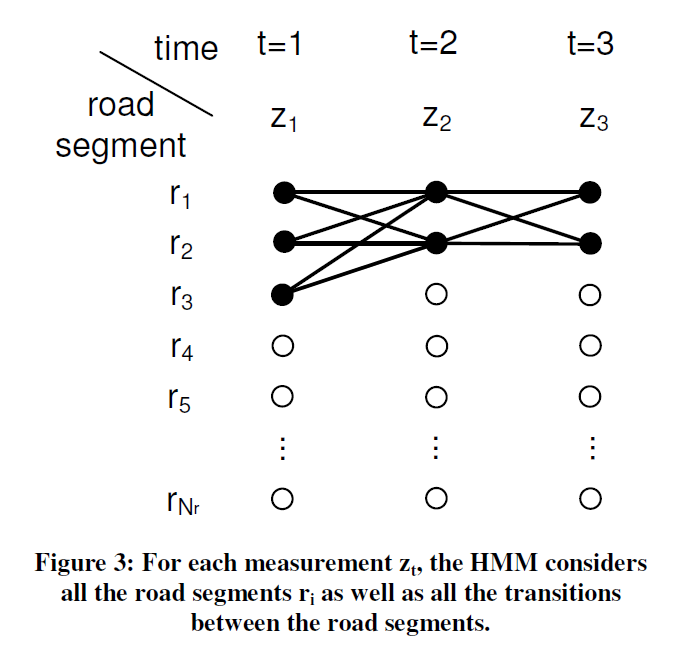
\includegraphics[scale=0.4  ]{hmm-hmm-of-observation.png}
\end{figure}

\begin{itemize}
    \item HMM状态:$ N_{r} $ individual  road  segments $ r_{i},  i=1 \ldots N_{r} $
    \item 状态的测量:每次带噪声的位置数据 $ Z_{t} $
    \item 候选路径:有很多,可能有很曲折的
    \item 目标:将每个GPS点匹配到合适的路段上
\end{itemize}

\subsection{已知在这个路段得到这个GPS点位置的概率估计}

\begin{figure}[h]
    \centering
    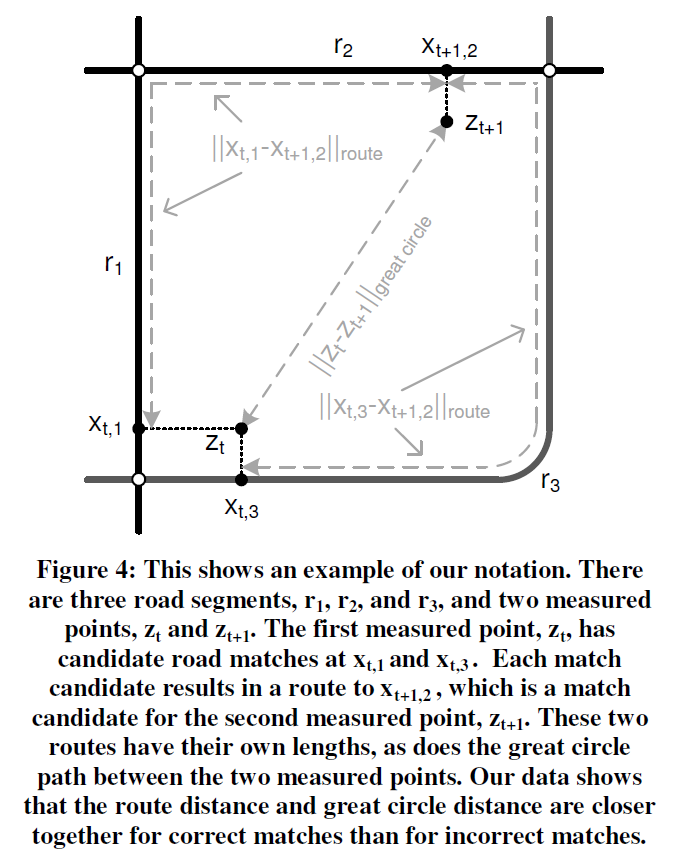
\includegraphics[scale=0.4  ]{HMM-mapping.png}
\end{figure}

对于给定的$z_{t},r_{i} $有\term{emission probability}$ x_{t, i}$。

估计方法:
The \term{great circle distance} on the surface of the earth between the measured point and the candidate match is $ \| z_{t}- x_{t, i} \|_{great\_circle}$. For the correct match, this difference is due to GPS noise. 噪声认为是零均值的高斯噪声。

$$ p\left(z_{t} \mid r_{i}\right)=\frac{1}{\sqrt{2 \pi} \sigma_{z}} e^{-0.5\left(\frac{\left\|z_{t}-x_{t, i}\right\|_{\text {great circle }}}{\sigma_{z}}\right)^{2}} $$

$\sigma_{z}$是GPS测量的方差(需要估计)。

对于初始状态$ \pi_{i} ,i=1 \ldots N_{r} $(指定一开始车辆在所有路段上的可能性),为了简化使用$$ \pi_{i}=p\left(z_{1} \mid r_{i}\right) $$

\subsection{转移概率}

Each measurement $ z_{t} $ has a list of possible road matches, as does the next measurement $ z_{t+1} $. 

作者认为\textbf{测量距离和大圆距离相近的状态转移才是比较好的},否则会绕路(概率下降)。

计算发现大圆距离与路径距离的差值绝对值近似于:

$$ p\left(d_{t}\right)=\frac{1}{\beta} e^{-d_{t} / \beta} $$

路径距离$ d_{t}=\left|\left\|z_{t}-z_{t+1}\right\|_{\text {great circle }}-\left\|x_{t, i^{*}}-x_{t+1, j^{*}}\right\|_{\text {route }}\right| $是动态规划(\term{Viterbi algorithm})得到的路线距离。对于$z_t$和候选路段$r_i$,匹配出在路段上的点是$ x_{t, i} $。

\begin{remark}
      \label{Comment:HMM-TransitionProbability}

      the transition probability
        dependence on the current and previous observations
    violates the properties of an ideal HMM

    the great-circle distance between
the observed locations may introduce significant errors in
estimating the circuitousness of a path (在定位误差大的情况下)

transition probabilities computed
based on the above measure of circuitousness vary greatly for
equally plausible transition paths depending on the sampling
interval
\end{remark}

\section{算法的实现}

\begin{itemize}
    \item 数据预处理的时候对于离上一个GPS点位置超过$ 2 \sigma_{z} $的点进行剔除
    \item 将离GPS位置观测值200米以外路段的观测概率设为0
    \item 对于大圆距离和路径距离超过2公里路径的观察概率设为0
    \item 对于明显超速的路径的概率设为0
    \item 当明显无法匹配的时候,移除一些点,尝试重新连接,如果仍旧无法连接,引入匹配断点
\end{itemize}

\subsection{参数估计}

估计GPS误差:
$ \sigma_{z} $ using the \term{median absolute deviation (MAD)}

$$ \sigma_{z}=1.4826 \mathrm{median}_{\mathrm{t}}\left(\left\|z_{t}-x_{t, i}\right\|_{\text {great circle }}\right) $$

the point on $ r_{i}^{*} $ (人工匹配的路段) nearest $ z_{t} $ is $ x_{t, i}^{*} $.

估计路径距离与大圆距离之间的差值:

$$ \begin{aligned} \beta=\frac{1}{\ln (2)} \operatorname{median}_{t} &\left(\mid\left\|z_{t}-z_{t+1}\right\|_{\text {great circle }}\right.\\ &\left.-\left\|x_{t, i^{*}}-x_{t+1, j} *\right\|_{\text {route }} \mid\right) \end{aligned} $$



\section{实验}

数据:真实驾车GPS数据、高斯噪声模拟数据

评价指标:reported error
  $$ \left(\mathrm{d}-+\mathrm{d}_{+}\right) / \mathrm{d}_{0} $$ 

  $d_{-}  $ =length erroneously subtracted,
  $ d_{+} $=length erroneously added

 

其他两种指标:

  Locations on Road. 
  \begin{remark}
      This accuracy measure
  says that the matched point should be in the
  same location as the actual vehicle. Since we
  measured the vehicle’s location with inherently
  noisy GPS, we do not know its actual location.
  \end{remark}

  Road Segment.
  \begin{remark}
      This accuracy measure says
  that the matched point should be on the same
  road segment as the actual vehicle. While the
  correct road segment is easier to guess than the
  correct location, it is still ambiguous at
  intersections, where a noisy measurement could
  match to any of the roads converging at that
  point.
  \end{remark}
  
   



\fi

\ifdefined\printcloudcomputing

\part{云计算}
\chapter{云计算基础}

\section{产生背景}

\subsection{云计算之前的技术}

\begin{definition}[并行计算]
    同时使用多种计算资源解决计算问题的过程,主要目的是快速解决大型且复杂的计算问题。

\end{definition}

并行计算把计算任务分派给系统内的多个运算单元。\term{HPC} server, 使用一个强大的机器或者infiniband 万兆网络连接,分派给系统中的多个运算单元;共享memory(可以直接访问所有内存)

\begin{definition}[InfiniBand]
    InfiniBand 是指具有非常高的RAS(可靠性、可用性、维护性)的基础设施/高性能计算机的服务器/集群用高速I/O总线架构及互联。作为系统间互联结构,除了RAS功能以外,与其他机构相比,具有低延迟这一点也是其特征。
\end{definition}

\begin{definition}[分布式计算]
    把一个需要巨大的计算能力才能解决的问题分成多个小部分,把这些小部分分配给多个计算进行处理,最后综合这些计算结果得到最终结果。
\end{definition}

分布式计算在cluster上运行,使用百兆网络等; 将计算任务分派给多个机器,再merge;分布式memory,需要进行消息传送

快速的分布式:MapReduce, Hadoop, spark

\begin{definition}[网格计算]
    利用互联网把地理上广泛分布的各种资源连成一个逻辑的整体,就像一台超级计算机一样。
\end{definition}

\begin{example}[教育网格]
    学校信息中心计算队列:将空闲的服务器通过教育网共享

    特点: 网格服务器一般不断电:软件configuration,路径,环境变量重启之后需要重新设置麻烦;逻辑上分布在不同机器上的程序是连续的,初期教育网格没有进行虚拟化
    缺点: 需要提供自己的计算资源,限制成员
\end{example}

\begin{definition}[云计算]
    一种基于互联网的计算方式. 通过网络,提供按需、且易扩展的弹性计算以及应用服务。
\end{definition}

云计算有anyone, anytime, anywhere的特点; 共享软硬件, 有些平台提供shared licenses的软件; 按需易拓展 autoscaling; 

\begin{figure}[htbp]
    \centering
    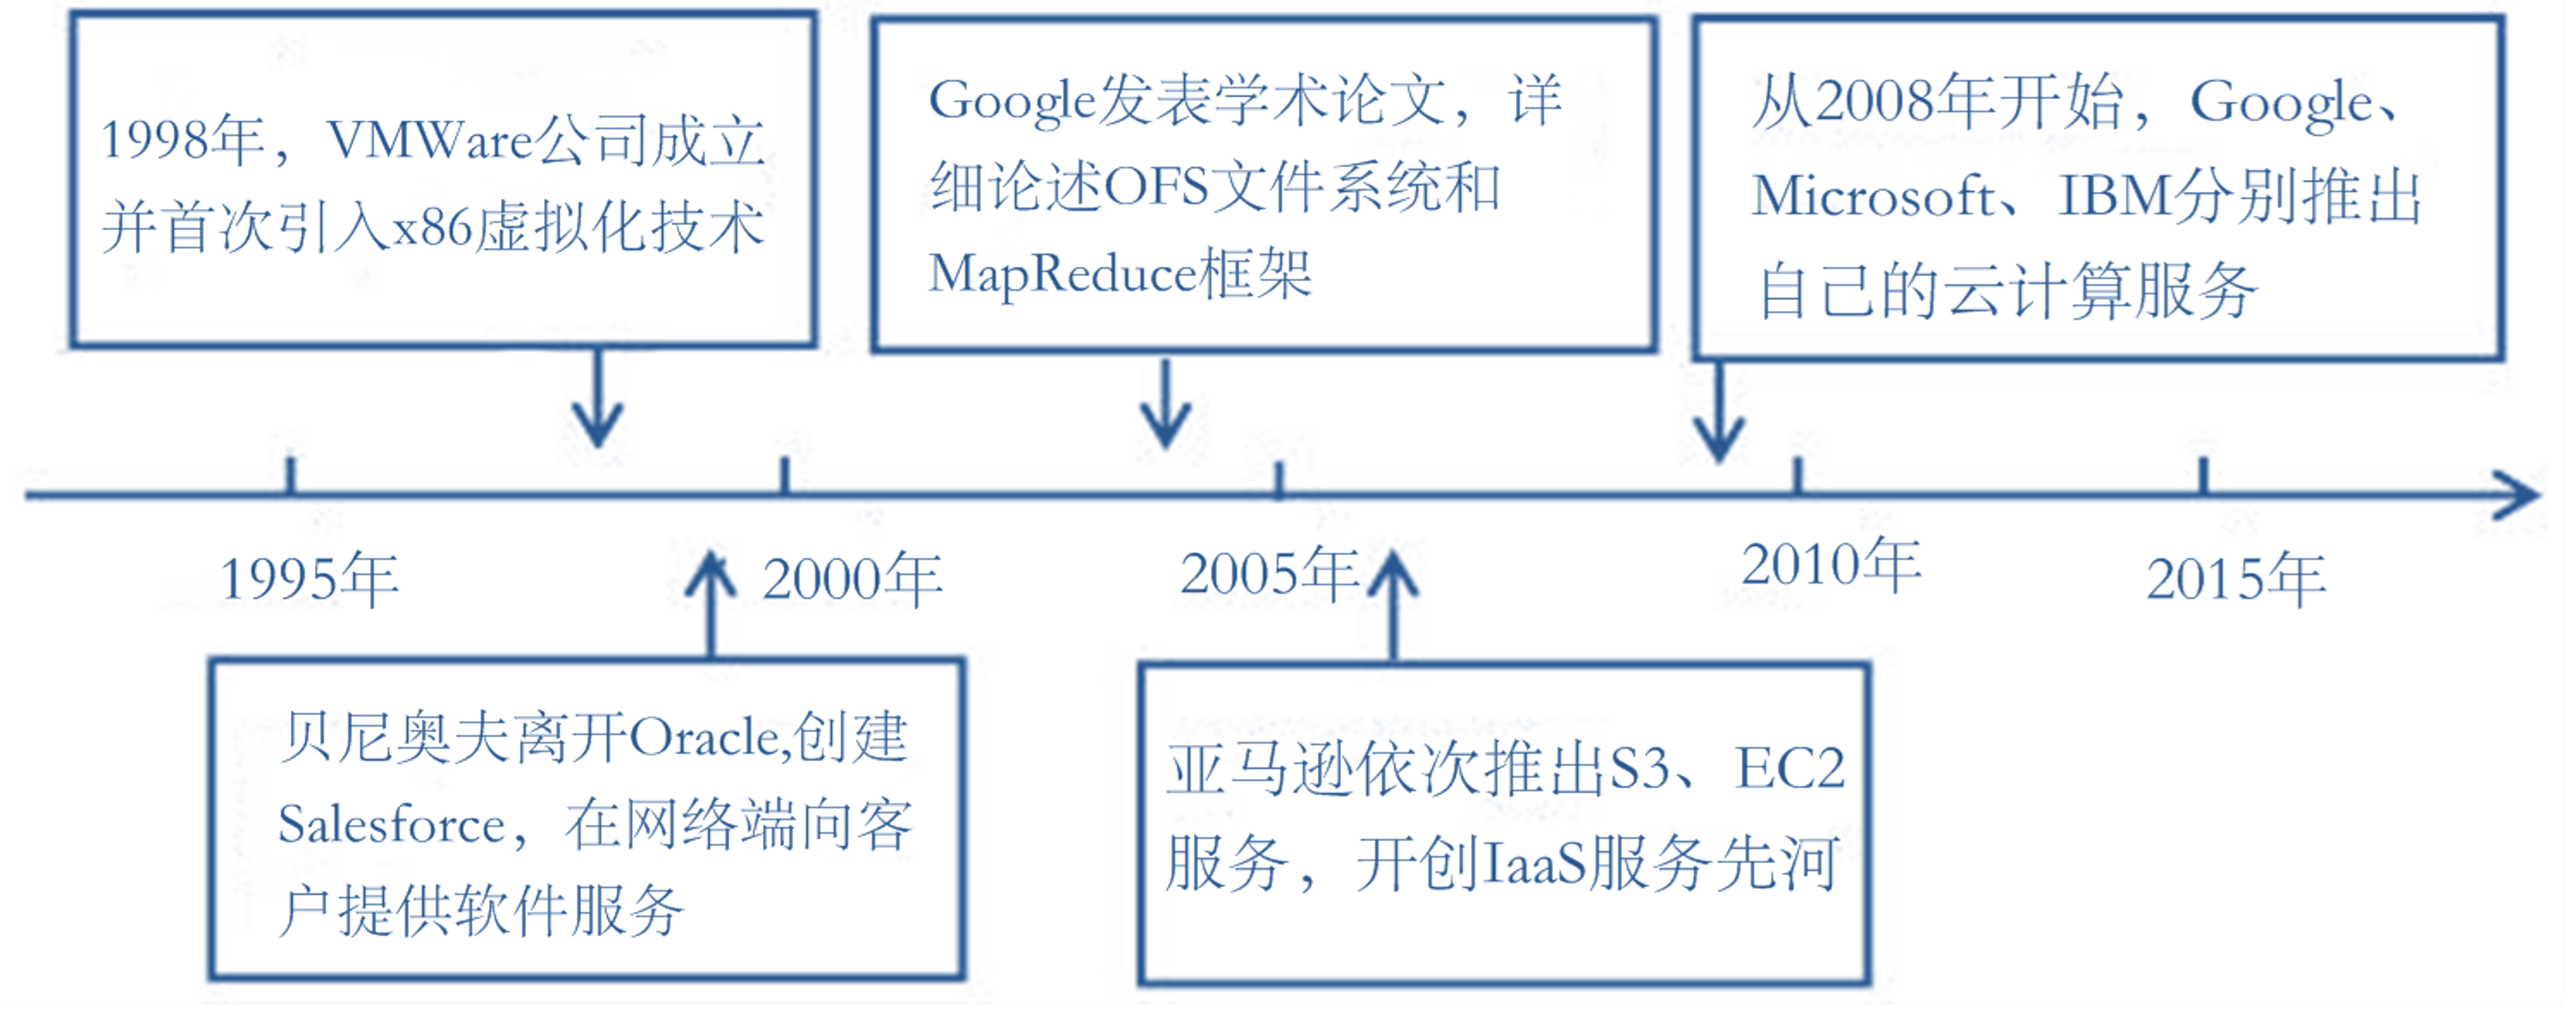
\includegraphics{cloud-development-of-cloud-computing.png}
\end{figure}

\subsection{其他技术的发展}

\begin{itemize}
    \item 5G
    \item 移动互联网
    \item 物联网
\end{itemize}

\subsection{国外云计算厂商}

亚马逊的云计算称为Amazon Web Services(AWS).率先在全球提供了弹性计算云EC2(Elastic Computing Cloud)和简单存储服务S3(Simple Storage Service),为企业提供计算和存储服务。收费的服务项目包括存储空间、带宽、CPU资源以及月租费。AWS服务的种类非常齐全. 
机器,计费使用时长(以小时, 分钟再到按照秒计算)等数据模型变化,技术不断进步.

\begin{definition}[Amazon Elastic Compute Cloud]
    Amazon Elastic Compute Cloud(Amazon EC2 云服务器)是一种 Web 云服务,能在云中提供安全且可调整大小的计算能力。该服务旨在让开发人员能够更轻松地进行 Web 规模的云计算。Amazon EC2 云服务器的 Web 云服务接口非常简单,您可以最小的阻力轻松获取容量,随之配置容量。使用该服务,您将能完全控制您的计算资源,并能在亚马逊成熟且行之有效的计算环境中运行。

    Amazon EC2 云服务器提供最广泛、最深入的计算平台,可选择处理器、存储、联网、操作系统和购买模式。我们提供最快的云处理器,是唯一的 400 Gbps 以太网网络云。我们拥有最强大的针对机器学习培训和图形工作负载的 GPU 云服务器实例,以及云中每次推理成本最低的云服务器实例。与任何其它云相比,AWS 均运行更多的 SAP、HPC、机器学习和 Windows 工作负载。单击此处了解 Amazon EC2 云服务器的最新功能。
\end{definition}

\begin{definition}[Serverless]
    开发者再也不用过多考虑服务器的问题,计算资源作为服务而不是服务器的概念出现。Serverless是一种构建和管理基于微服务架构的完整流程.

    (AWS 上的无服务器)无服务器是一种用于描述服务、实践和策略的方式,使您能够构建更敏捷的应用程序,从而能够更快地创新和响应变化。凭借无服务器计算,容量预置和补丁等基础设施管理任务由 AWS 处理,以便您能够专注于编写为客户服务的代码。AWS Lambda 等无服务器服务具有自动扩展、内置高可用性以及按价值付费的计费模型。Lambda 是一种事件驱动的计算服务,使您能够运行代码来响应来自 200 多个本地集成的 AWS 和 SaaS 源的事件 — 所有这些都无需管理任何服务器。
\end{definition}

\begin{definition}
    AWS Lambda 是一种无服务器的计算服务,让您无需预置或管理服务器、创建可感知工作负载的集群扩展逻辑、维护事件集成或管理运行时,即可运行代码。借助 Lambda,您几乎可以为任何类型的应用程序或后端服务运行代码,而且完全无需管理。只需将您的代码以 ZIP 文件或容器映像的形式上传,Lambda 便会自动、精确地分配计算执行能力,并根据传入的请求或事件运行您的代码,以适应任何规模的流量。您可以将您的代码设置为自动从 200 多个 AWS 服务和 SaaS 应用程序触发,或者直接从任何 Web 或移动应用程序调用。您可以使用自己喜欢的语言(Node.js、Python、Go、Java 等)编写 Lambda 函数,并使用无服务器和容器工具(例如 AWS SAM 或 Docker CLI)来构建、测试和部署您的函数。
\end{definition}

\begin{definition}[(腾讯云)云函数]
    腾讯云云函数是腾讯云提供的 Serverless 执行环境。您只需编写简单的、目的单一的云函数即可将它与您的腾讯云基础设施及其他云服务产生的事件关联。

使用云函数时,您只需使用平台支持的语言(Python、Node.js、PHP、Golang、Java 及 Custom Runtime)编写代码。腾讯云将完全管理底层计算资源,包括服务器 CPU、内存、网络和其他配置/资源维护、代码部署、弹性伸缩、负载均衡、安全升级、资源运行情况监控等。但这也意味着您无法登录或管理服务器、无法自定义系统和环境。

云函数自动地在同一地域内的多个可用区部署,同时提供极高的容错性。云函数在执行时将根据请求负载扩缩容,从每天几个请求到每秒数千个请求,都由云函数底层自行伸缩。您无需人工配置和介入,只需为运行中的云函数付费,即可满足不同情景下服务的可用性和稳定性。若云函数未运行,则不产生任何费用。

您可以自定义运行云函数的时机,例如,在 COS Bucket 上传时、删除文件时运行云函数、使用 Ckafka 中的消息时运行云函数、应用程序通过 SDK 调用时运行云函数,或指定云函数定期执行。您可以使用云函数作为 COS 服务的数据处理触发程序轻松实现 IFTTT 逻辑,您也可以通过构建灵活的定时自动化任务,用于覆盖手工完成的操作,轻松构建灵活可控的软件架构。

\begin{itemize}
    \item 简单易用: 用户只需编写最重要的“核心代码”,不再需要关心周边组件,极大地降低了服务架构搭建的复杂性。无需任何手动配置,云函数即可根据请求量自动横向扩缩。不管您的应用每天的请求数处于波峰还是波谷,云函数均可自动安排合理的计算资源满足业务需求。
    \item 高效: 云函数不要求特定框架,开发者可专注于核心代码的开发。单个模块的开发无需了解代码细节。您可以使用云函数编写一些目的单一、逻辑独立的业务模块。每个函数都是单独运行、单独部署、单独伸缩的,用户上传代码后即可自动部署,提升了独立开发和迭代的速度。
    \item 稳定可靠: 如果某个可用区因灾害或电力故障等导致瘫痪,云函数会自动地选择其他可用区的基础设施来运行,免除单可用区运行的故障风险。由事件触发的工作负载可以使用云函数来实现,利用不同云服务满足不同的业务场景和业务需求,使得您的服务架构更加健壮。
    \item 简化管理: 用户不再需要对 OS 入侵、登录风险、文件系统安全、网络安全和端口监听做复杂的配置和管理,一切交由平台处理,平台通过定制化的容器保证每个用户的隔离性。用户无需复杂的配置文件即可一键部署和测试云函数。
    \item 降低开销: 云函数在未执行时不产生任何费用,所以对一些无需常驻的业务进程来说,开销将大幅降低。云函数执行时按请求数和计算资源的运行时间收费,价格优势明显,对初创期的开发者十分友好。
\end{itemize}
\end{definition}

谷歌是最大的云计算技术的使用者. 谷歌已经允许第三方在谷歌的云计算中通过\term{Google App Engine}运行大型并行应用程序. 发表学术论文的形式公开其云计算三大法宝:\term{Google File System} (GFS)、\term{MapReduce}和\term{BigTable}. 基于TensorFlow


微软紧跟云计算步伐,推出了Microsoft Azure. 微软将为Windows Azure用户推出许多新的功能,不但能更简单地将现有的应用程序转移到云中,而且可以加强云托管应用程序的可用服务,充分体现 出微软的“云”+“端”战略。在中国,微软2014年3月27日宣布由世纪互联负责运营的Microsoft Azure公 有云服务正式商用,这是国内首个正式商用的国际公有云服务平台。

\begin{figure}[htbp]
    \centering
    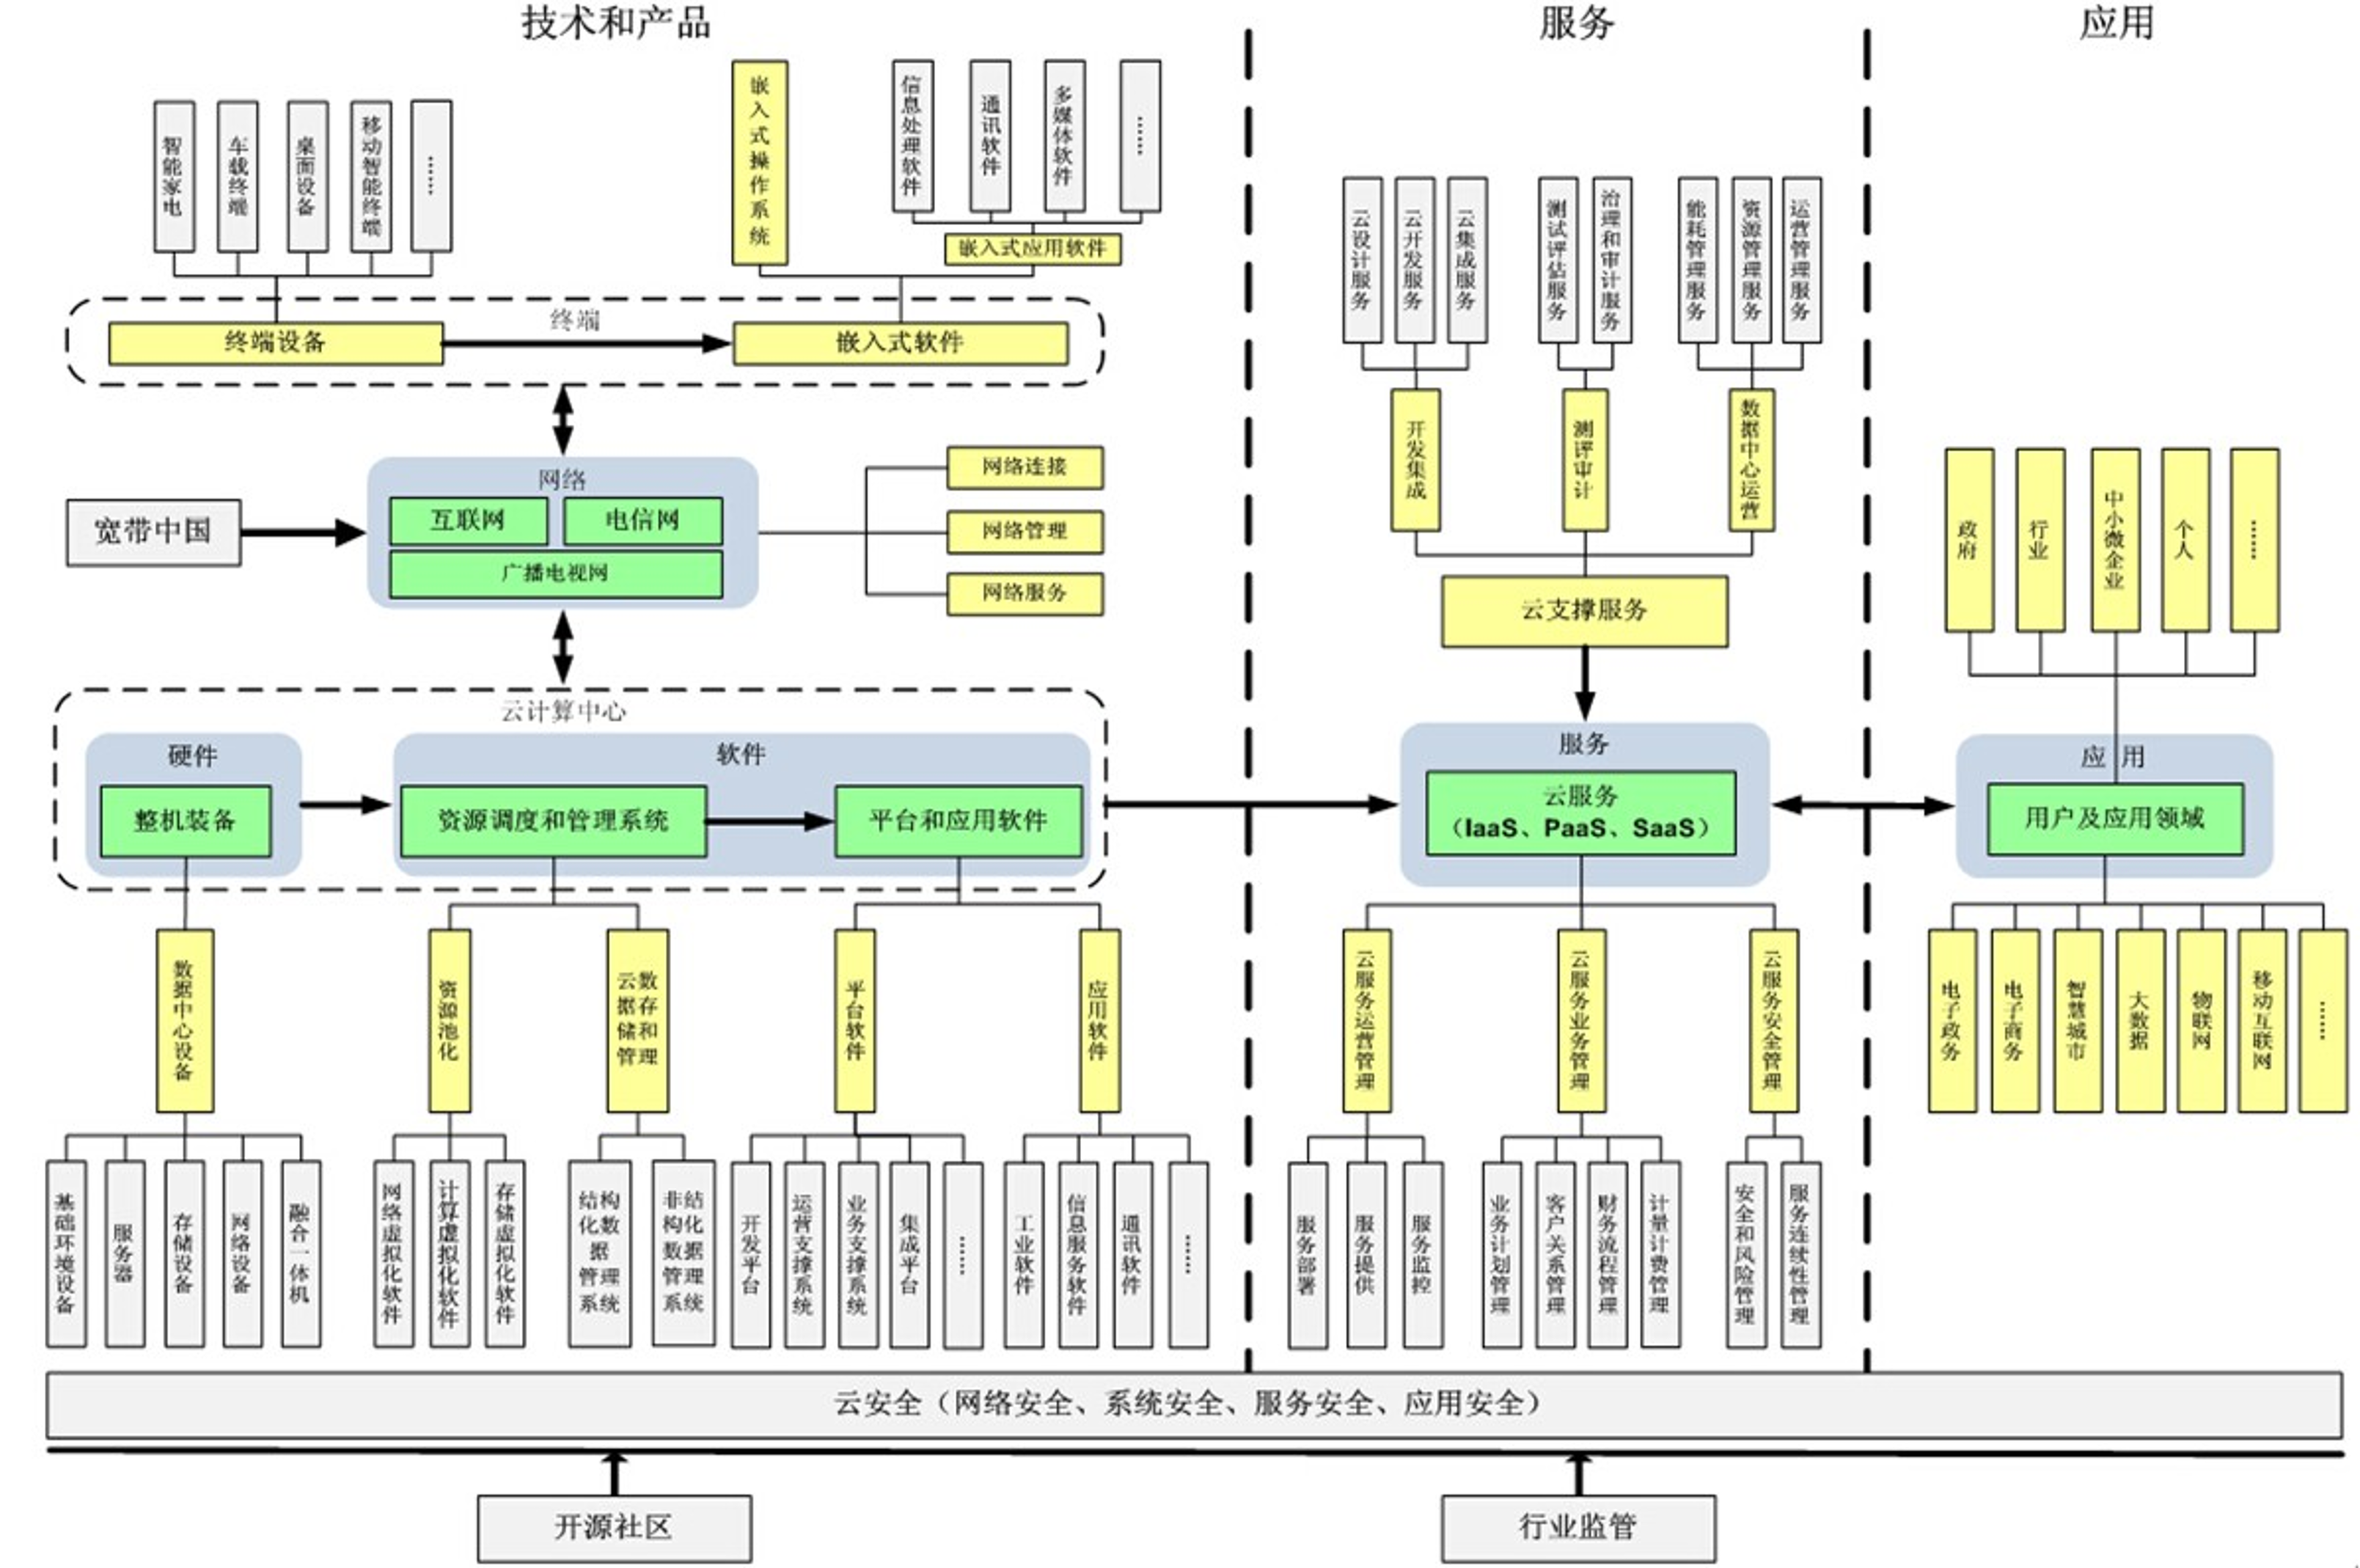
\includegraphics{cloud-cloud-computing-biosphere.png}
\end{figure}

\subsection{其他原因}

个人使用计算机的不灵活性:

\begin{itemize}
    
    
    \item 刚高价购买的最新版的应用程序,过了不久就需要进行更新
    \item 你刚刚购买完电脑,就出现了新的型号
    \item 电脑因为太多的不灵活的软件,负载过重而宕机,导致保存的数据全部丢失
    \item 一时冲动购买了一套软件,结果用了不到一个月就失去了兴趣
\end{itemize}

企业使用计算机的不灵活性:

\begin{itemize}
    
    
    \item IT部门的工作人员经常忙于穿梭于各个办公楼之间解决员工电脑的各种系统错误,各种应用软件的错误
    \item 企业为了测试新开发的应用软件,需要购买一大批电脑,而当测试完毕之后,大部分设备处于闲置
    \item 为了应付市场的快速变化,急需一批计算资源,但是审批资金、购买设备、安装平台可能需要花费2周左右的时间,会耽误市场机会
    \item 高价购买了某家公司的软件之后,使用一段时间之后,发现不能完全满足需求,但是又无法退货
\end{itemize}

云计算提出前的互联网遇到的难题:
\begin{itemize}
    \item \textbf{互联网上的数据量高速增长}(\term{Big Data}),导致了互联网数据处理能力的不足;
    \item 互联网上存在着大量处于闲置状态的计算设备和存储资源;
    \item 服务器更新换代速度加快,企业升级费用昂贵。
\end{itemize}

\section{云计算与大数据}

\begin{definition}[Big Data]
    海量数据或巨量数据,其规模巨大到无法通过目前主流的计算机系统在合理时间内获取、存储、管理.
\end{definition}

\subsection{大数据的特征}

\begin{itemize}
    \item 价值密度低(Value):(需要挖掘数据,数据清洗:重复、无用、噪声数据、缺失值处理)在成本可接受的条件下,通过快速采集、发现和分析,从大量、多种类别的数据中提取价值的体系架构。

    \item 快速(Velocity):数据增长速度快,而且越新的数据价值越大,这就要求对数据的处理速度也要快,以便能够从数据中及时地提取知识,发现价值。(产生速度快,数据处理需要高效率) 例如\term{Streaming Processing}:如果处理速率不够快,会\term{丢包}; zoom 多方会议,带宽有限,如何进行数据传输调度?$\rightarrow$用户体验提升

    \item 数据量大(Volume):存储的数据量巨大,PB级别是常态,因而对其分析的计算量也大。

    \item  多样(Variety):数据的来源及格式多样,数据格式除了传统的结构化数据外,还包括\term{半结构化数据}或\term{非结构化数据}(如搜索喜马拉雅:只能搜索\term{metadata}(文件名/小说名/属性等),无法根据内容中的某个细节搜索 $\rightarrow$ \term{非结构化数据索引})。而随着人类活动的进一步拓宽,数据的来源更加多样。

   \item 复杂度(Complexity):对数据的处理和分析的难度大。

   $$G=f(x), f:\text{云计算}, x:\text{大数据}$$
\end{itemize}



\section{云计算基本思想 (通用性)}

\begin{itemize}
    \item 基本能力(所有的计算能力、存储能力、和各种各样功能的应用)都可通过网络获得
    \item 云应对用户硬件友好, 不需要不停地更换昂贵的高性能电脑
    \item 不需要用户安装复杂软件
    \item  数据保证安全(备份)
\end{itemize}

\term{三备份},仍旧可能会丢失
\chapter{云计算关键技术}

\section{虚拟化}

\begin{definition}[虚拟化]
    通过该技术将一台计算机虚拟为多台逻辑计算机。 在一台计算机上同时运行多个逻辑计算机,每个逻辑计算机可运行不同的操作系统,并且应用程序都可以在相互独立的空间内运行而互不影响,从而显著提高计算机的工作效率。 
\end{definition}

\begin{example}[Amazon开启虚拟机]
    选择ami(guest OS image):支持的virtualization type (\term{paravirtual} 半虚拟化 $\rightarrow$ 性能不一致)
\end{example}

\begin{figure}
    \centering
    \begin{subfigure}[b]{0.3 \textwidth}
        \centering
        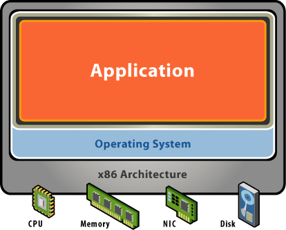
\includegraphics[width=\textwidth]{cloud-pc-architecture.png}
    \end{subfigure}
    \begin{subfigure}[b]{0.3 \textwidth}
        \centering
        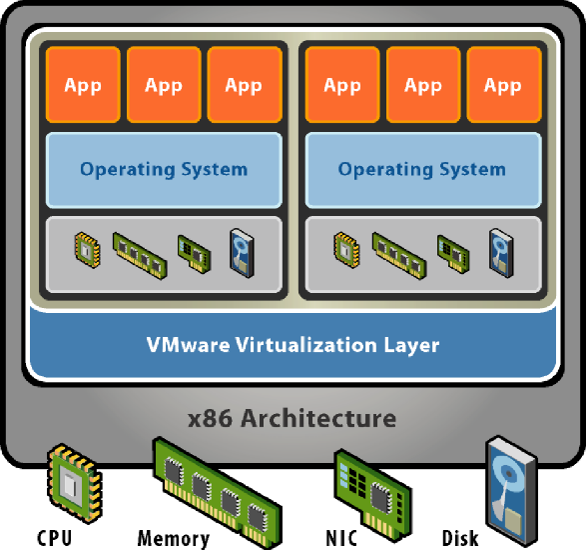
\includegraphics[width=\textwidth]{cloud-vmware-architecture.png}
    \end{subfigure}
\end{figure}

\begin{definition}[Host Machine]
    物理机
\end{definition}

\begin{definition}[Host OS]
    运行在物理机之上的OS
\end{definition}

\begin{definition}[Hypervisor, Virtual Machine Monitor (VMM)]
    虚拟机监控器
\end{definition}

\begin{definition}[Virtual Machine]
    虚拟出来的虚拟机
\end{definition}

\begin{definition}[Guest OS]
    运行在虚拟机之上的OS
\end{definition}

假如一个核分给2个虚拟机,则平台,OS需要分时切换。️ 网络的虚拟化隔离难以实现,因此虚拟化机网络性能不稳定, 虚拟机的网络转发到物理机的网络中。

虚拟化特点:

\begin{itemize}
    \item 分区: 在单一物理服务器上同时运行多个虚拟机
    \item 隔离: 在同一服务器上的虚拟机相互隔离
    \item 封装: 整个虚拟机都保存在文件中,而且可以通过移动和复制这些文件的方式来移动和复制该虚拟机
\end{itemize}

虚拟机上读取数据? 

硬件磁盘挂载在硬件上 guest OS转换请求到hypervisor$\rightarrow$ OS$\rightarrow$ 硬件以隔离不同虚拟机,overhead大

\subsection{从虚拟平台角度划分的分类}

\subsubsection{全虚拟化}

\begin{definition}[全虚拟化]
    虚拟的操作系统,与底层的硬件完全隔离,由中间的Hypervisor层转化。 
    
    典型的代表有Vmware WorkStation, Microsoft Virtrual Server. 
\end{definition}

\begin{definition}[KVM]
    KVM (for Kernel-based Virtual Machine) is a full virtualization solution for Linux on x86 hardware containing virtualization extensions (Intel VT or AMD-V). It consists of a loadable kernel module, kvm.ko, that provides the core virtualization infrastructure and a processor specific module, kvm-intel.ko or kvm-amd.ko
\end{definition}

完全隔离,由hypervisor层转换 

VMware workstation:速度减慢,性能瓶颈,隔离更好

\subsubsection{半虚拟化}

\begin{definition}[半虚拟化]
    虚拟机的操作系统当中加入特定的虚拟化指令,可以\textbf{直接通过Hypervisor调用硬件资源},免除了Hypervisor层转换指令的开销。 
    
    典型代表有Xen, Hyper-V
\end{definition}

使得OS和虚拟化层协同工作,减轻2层OS的负担,但是需对OS进行改动,OS知道正处于虚拟化环境中,开销减小

xen(也逐渐支持全虚拟化,以提升通用性)

\begin{definition}[Xen]
    The Xen Project community develops an open-source type-1 or bare-metal hypervisor, which makes it possible to run many instances of an operating system or indeed different operating systems in parallel on a single machine (or host). The project develops the only type-1 hypervisor that is available as open source. The hypervisor is used as the basis for a number of different commercial and open source applications, such as server virtualization, Infrastructure as a Service (IaaS), desktop virtualization, security applications, embedded and hardware appliances, and automotive. It enables users to increase server utilization, consolidate server farms, reduce complexity, and decrease total cost of ownership.
\end{definition}

\subsection{从虚拟化的层次划分}

\subsubsection{软件辅助的虚拟化技术}

\begin{definition}[软件辅助的虚拟化技术]
    通过软件的方法,让客户机的特权指令陷入异常,从而触发宿主机进行虚拟化。 如Hyper-V等。 
\end{definition}

\begin{definition}[Hyper-V]
    Hyper-V specifically provides hardware virtualization. That means each virtual machine runs on virtual hardware. Hyper-V lets you create virtual hard drives, virtual switches, and a number of other virtual devices all of which can be added to virtual machines
\end{definition}

\subsubsection{硬件支持的虚拟化技术}

\begin{definition}[硬件支持的虚拟化技术]
    在X86处理系统架构中加入新的指令机以及运行模式完成虚拟化操作,进而对硬件资源进行直接调用,进行虚拟化。 如AMD-V等。 
\end{definition}

\subsection{从虚拟化的实现结构划分}

\subsubsection{基于操作系统的虚拟化}
\begin{definition}[基于操作系统的虚拟化]
    在一个已存在的操作系统上安装虚拟化软件

    特点:
    
    \begin{itemize}
        \item 简单、易于实现
        \item 安装和运行虚拟化程序依赖于主机操作系统对设备的支持
        \item 有两层OS,管理开销较大,性能损耗大
        \item 虚拟机对各种物理设备的调用,都通过虚拟化层和宿主机的OS一起协调才能完成
    \end{itemize}

    例子:Vmware Workstation和VirtualBox等
\end{definition}

2层OS,易于实现,开销较大,需要管理层OS层转换请求 

如VMware

\subsubsection{基于硬件的虚拟化}

\begin{definition}[基于硬件的虚拟化]
    将虚拟化软件直接安装在物理主机硬件上。 

    特点:
    \begin{itemize}
        \item 不依赖于主机操作系统
        \item 支持多种操作系统,多种应用
        \item 依赖虚拟化层进行管理
        \item 需要对虚拟层内核进行开发
    \end{itemize}

例子:VMvare ESX、Xen等
\end{definition}

省略OS层 如xen,依赖虚拟化层进行管理,不依赖于主机OS,可直接调用硬件 缺点:依赖于虚拟化层,需要对虚拟化层进行开发, 

如 VMware ESXi, XEN

\begin{definition}[VMware ESXi]
    The Purpose-Built Bare Metal Hypervisor
Discover a robust, bare-metal hypervisor that installs directly onto your physical server. With direct access to and control of underlying resources, VMware ESXi effectively partitions hardware to consolidate applications and cut costs. It's the industry leader for efficient architecture, setting the standard for reliability, performance, and support.
\end{definition}

\begin{definition}[Xen]
    the xen project is focused on advancing virtualization in a number of different commercial and open source applications, including server virtualization, infrastructure as a services (iaas), desktop virtualization, security applications, embedded and hardware appliances, and automotive/aviation
\end{definition}

\begin{definition}[Hardware Virtual Machine]
    HVM (known as Hardware Virtual Machine) is the type of instance that mimics bare-metal server setup which provides better hardware isolation. 
    
    With this instance type, the OS can run directly on top of the Virtual Machine without additional configuration making it to look like it is running on a real physical server. For more information about this instance type and the other one that is most commonly used, you may refer to the resource link below.
\end{definition}

\begin{remark}
    Windows不支持HVM.
\end{remark}

研究方向:云计算虚拟化,如live migration(实时虚拟机迁移:无感迁移?)


\subsection{从虚拟化在云计算的应用领域进行划分}
\begin{definition}[服务器虚拟化]
    将一台服务器虚拟成多台服务器进行使用

    对资源池的巨大文件系统管理 
  存储资源统一整合管理:目录树🌲管理
  🔀底层实现高效组织,保持隔离,
多‍‍‍读写同一台机器性能瓶颈(用户行为特征:经常读的用户,经常写的用户,调度)
\end{definition}

\begin{definition}[存储虚拟化]
    将整个云系统的存储资源进行统一整合管理
\end{definition}

\begin{definition}[应用程序虚拟化]
    把应用程序对底层硬件和系统的依赖抽取出来,从而解耦
\end{definition}

\begin{definition}[平台虚拟化]
    集成各种开发资源虚拟出一个面向开发人员的统一接口,如监控视频平台、消息平台、短信平台
\end{definition}

\begin{definition}[桌面虚拟化]
    将用户的桌面以使用的终端进行分离,进行解耦

    桌面和terminal解耦
\end{definition}

\section{虚拟化技术}


\subsection{完全虚拟化技术}

\begin{definition}[完全虚拟化技术]
    通过hypervisor在虚拟服务器和底层硬件之间建立一个抽象层。 
\end{definition}

最流行的虚拟化方法使用hypervisor,在虚拟服务器和底层硬件之间建立一个抽象层。 VMware和微软的VirtualPC是代表该方法的两个商用产品,而基于核心的虚拟机(KVM)是面向Linux系统的开源产品。 

hypervisor可以捕获CPU指令,为指令访问硬件控制器和外设充当中介。 因而,完全虚拟化技术几乎能让任何一款操作系统不用改动就能安装到虚拟服务器上,而它们不知道自己运行在虚拟化环境下。 主要缺点是, hypervisor给处理器带来开销。 


\subsection{准虚拟化技术}

\begin{definition}[准虚拟化技术]
    完全虚拟化是处理器密集型技术,因为它要求hypervisor管理各个虚拟服务器,并让它们彼此独立。 减轻这种负担的一种方法就是,改动客户操作系统,让它以为自己运行在虚拟环境下,能够与hypervisor协同工作。 这种方法就叫\textit{准虚拟化(para-virtualization)}. 
\end{definition}

Xen是开源准虚拟化技术的一个例子。 操作系统作为虚拟服务器在Xen hypervisor上运行之前,它必须在核心层面进行某些改变。 因此, Xen适用于BSDLinux, Solaris及其他开源操作系统,但不适合对像Windows这些专有的操作系统进行虚拟化处理,因为它们无法改动。 

准虚拟化技术的优点是性能高。 


\subsection{CPU虚拟化技术}


\begin{definition}[CPU虚拟化技术]
    一个core$\rightarrow$ 一个虚拟机。
\end{definition}

CPU的虚拟化技术可以单CPU模拟多CPU并行,允许一个平台同时运行多个操作系统,并且应用程序都可以在相互独立的空间内运行而互不影响,从而显著提高计算机的工作效率。 

\begin{definition}[virtual CPUs]
    与硬件无关
\end{definition}

\begin{definition}[core, locigal CPU]
    逻辑处理器
\end{definition}

\begin{definition}[hyperthread]
    一个核变2个核(某些硬件存在2份,如registers,加快运算单元运算,一个线程block时执行另一线程)
\end{definition}

\begin{remark}
    虚拟CPU性能取决于2级调度的效率。

    guest application$\rightarrow$ 虚拟CPU调度
    虚拟CPU发出指令$\rightarrow$ vmm调度$\rightarrow$ 物理核(任务队列)

    \begin{figure}[htbp]
        \begin{center}
            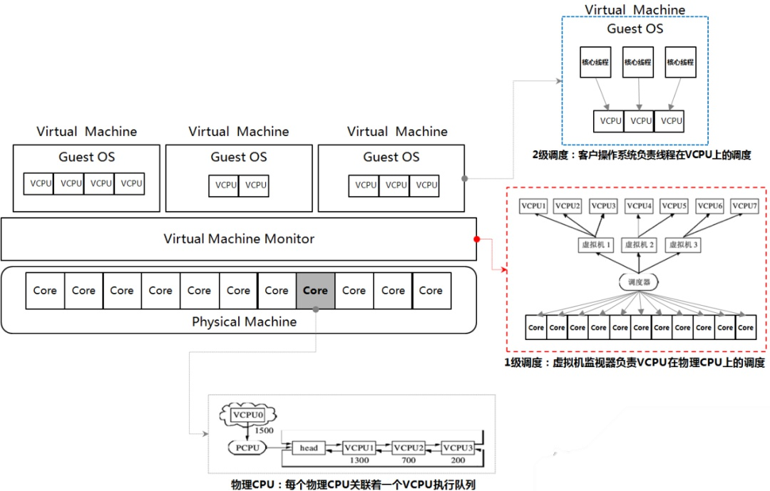
\includegraphics[width=\textwidth]{cloud-cpu-virtualization.png}
        \end{center}
    \end{figure}
\end{remark}



\subsection{CPU全虚拟化}
主要采用优先级压缩技术(\term{Ring Compression})和二进制代码翻译技术Binary Translation) . 优先级压缩技术让VMM和Guest运行在不同的特权级下。 

对X86架构而言,即VMM运行在最高特权级别Ring 0下, Guest OS运行在Ring 1下,用户应用运行在Ring 3下。 因此Guest OS的核心指令\textbf{无法直接下达到计算机系统硬件执行},而是需要经过VMM的\textbf{捕获}和\textbf{模拟}执行(部分难以虚拟化的指令需要通过\term{Binary Translation}技术进行转换) . 

\begin{figure}[htbp]
    \begin{center}
        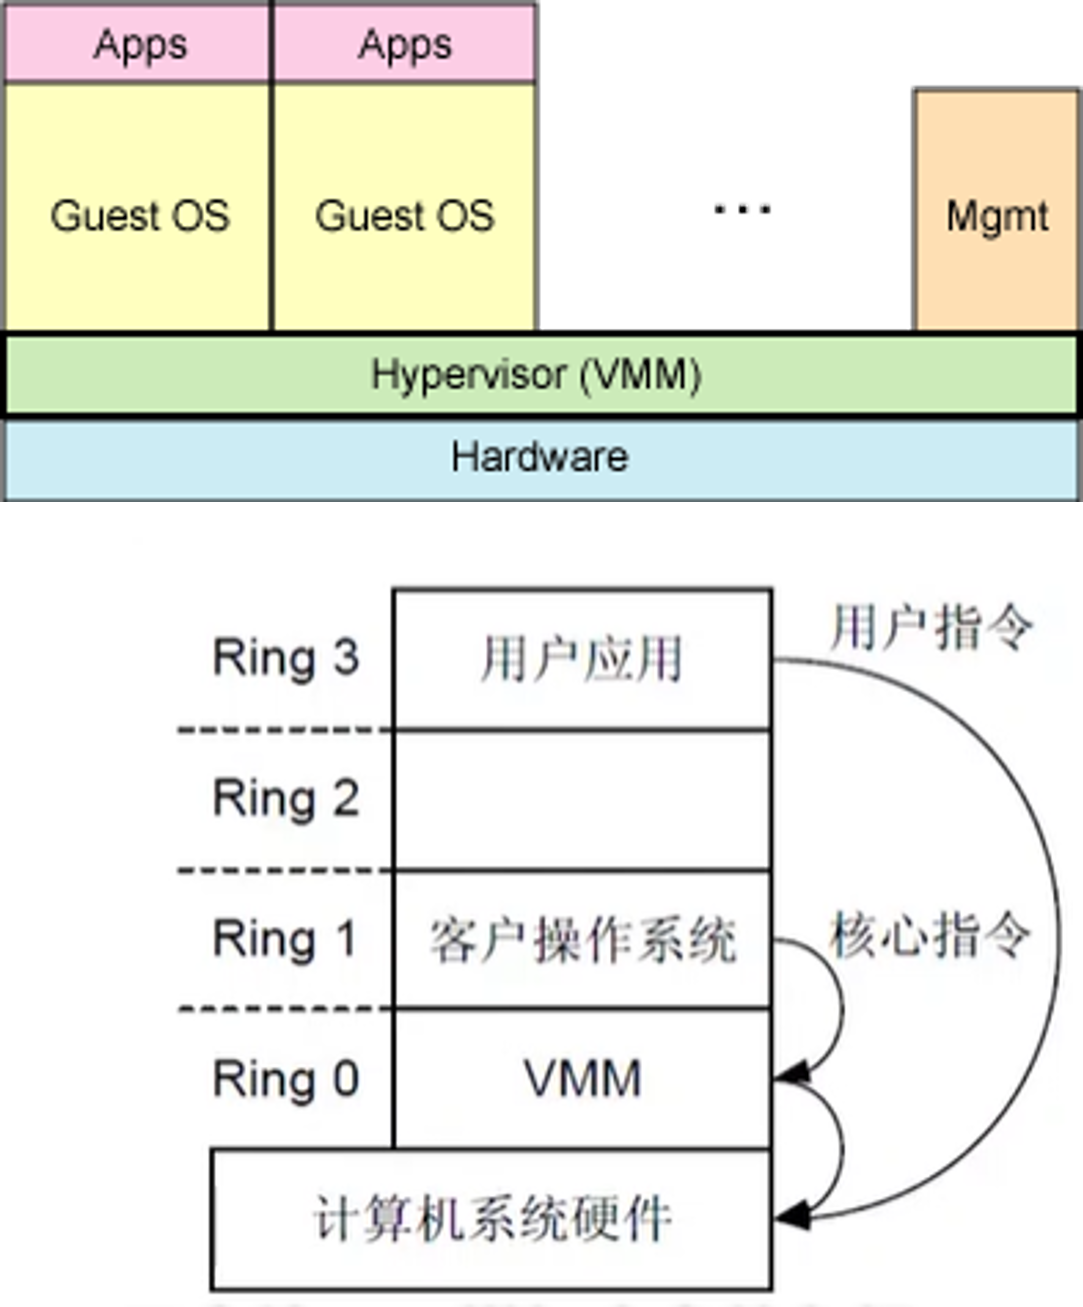
\includegraphics[]{cloud-cpu-full-virtualization.png}
    \end{center}
\end{figure}

\subsection{CPU半虚拟化}
    
主要采用\term{Hypercall}技术。 

\textbf{Guest OS的部分代码被改变},从而使Guest OS会将和特权指令相关的操作都转换为发给VMM的Hypercall (超级调用) ,由VMM继续进行处理。 而Hypercall支持的批处理和异步这两种优化方式,使得通过Hypercall能得到近似于物理机的速度。 

\begin{figure}[htbp]
    \begin{center}
        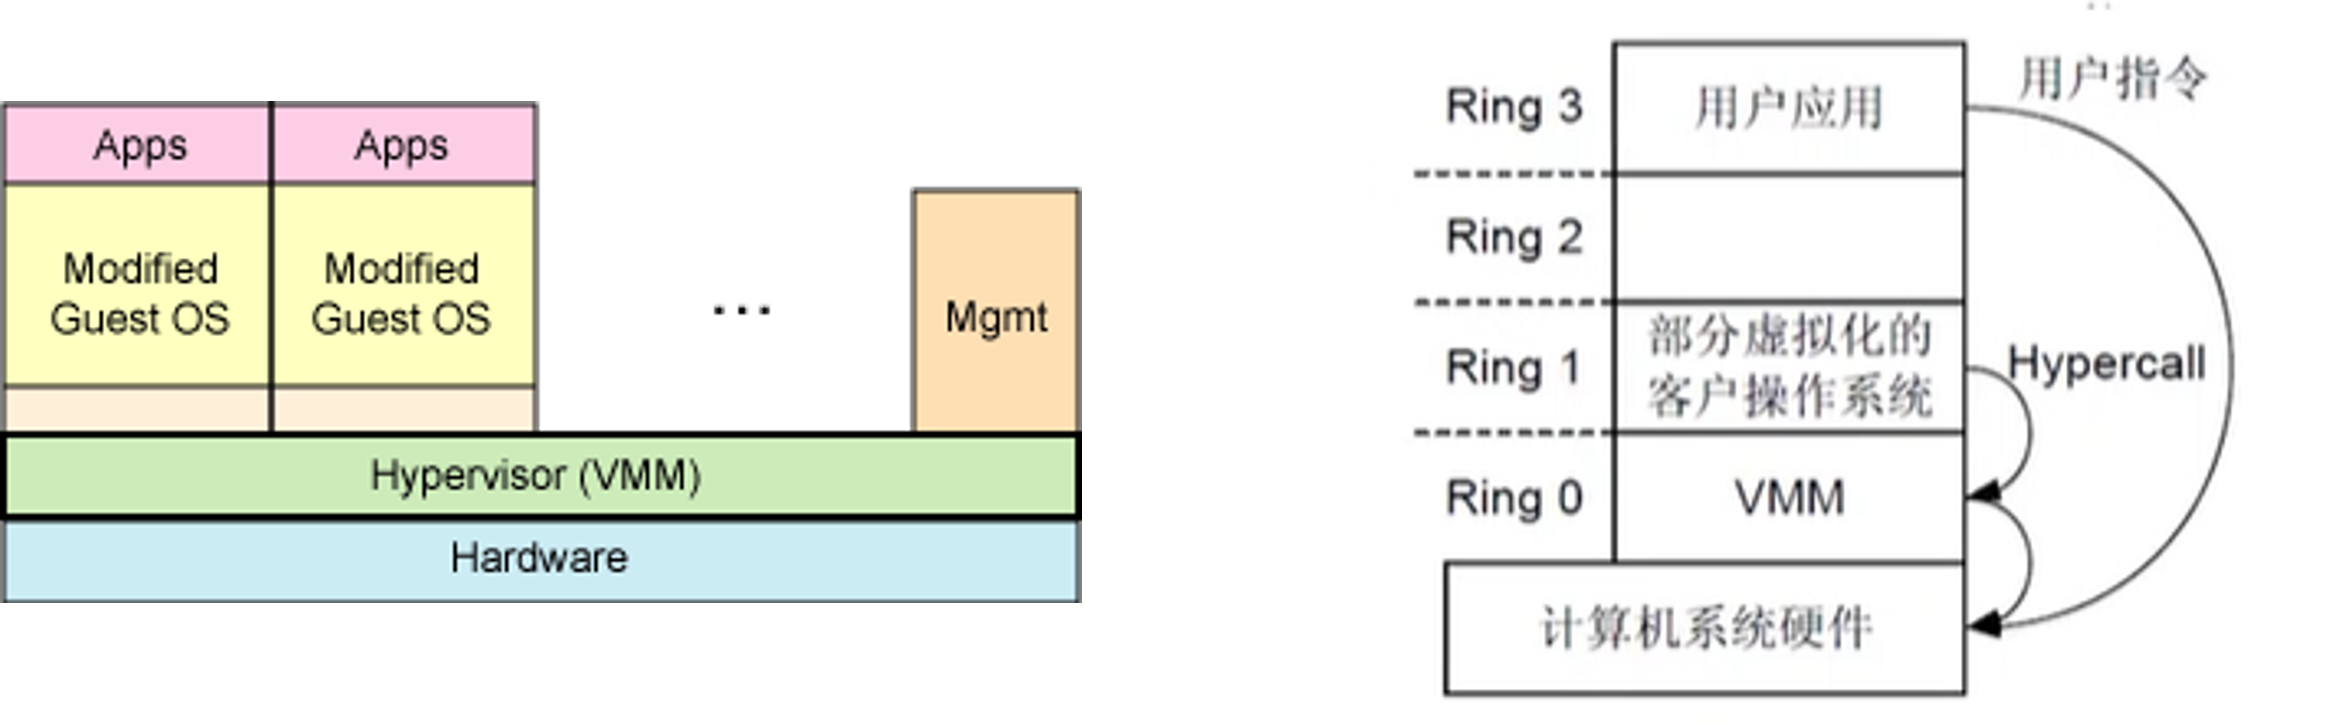
\includegraphics[width=\textwidth]{cloud-cpu-para-virtualization.png}
    \end{center}
\end{figure}

\subsection{CPU硬件辅助虚拟化技术}

目前主要有Intel的\term{VT-x}和AMD的\term{AMD-V}这两种技术。 

其核心思想都是通过引入新的指令和运行模式,使VMM和Guest OS分别运行在不同模式(\term{Root模式}和非ROOT模式)下,且Guest OS运行在Ring 0下。 通常情况下, Guest OS的核心指令可以直接下达到计算机系统硬件执行,而不需要经过VMM,当Guest OS执行到特殊指令的时候,系统会切换到VMM,让VMM来处理特殊指令。 

区分root模式, monitor运行在root模式运行,虚拟机支持非root的ring0,硬件区分来自guest OS指令和host OS指令,核心指令可以直接发送给CPU而无需vmm捕捉

\begin{figure}[htbp]
    \begin{center}
        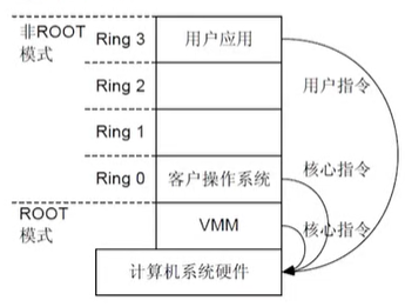
\includegraphics[]{cloud-cpu-assisted-virtualization.png}
    \end{center}
\end{figure}

\subsection{内存虚拟化技术}

内存虚拟化技术的产生:内存虚拟化的产生源于VMM与客户系统在对物理内存的认识上存在冲突,造成物理内存真正拥有者-VMM必须对系统访问的内存进行一定程度上的虚拟化。 

虚拟机的内存映射到真实存储器的顺序: 真实物理内存$\rightarrow$ 其他存储,️超过物理内存时performance下降

$虚拟地址\leftrightarrow^{translation}实际地址$

每个进程看到独立的地址内存空间
假如超过内存空间,需等待其他程序释放

虚拟地址 $\leftrightarrow$ real memory address(虚拟机所看到的虚拟地址) $\leftrightarrow$ physical(物理机看到的虚拟地址)

\subsubsection{内存全虚拟化技术}

通过使用影子页表(Shadow Page Table)实现虚拟化。 

VMM为每个Guest都维护一个影子页表,影子页表维护虚拟地址(VA)到机器地址(MA)的映射关系。 而Guest页表维护VA到客户机物理地址(GPA)的映射关系。 

当VMM捕获到Guest页表的修改后, VMM会查找负责GPA到MA映射的P2M页表或者哈希函数,找到与该GPA对应的MA,再将MA填充到真正在硬件上起作用的影子页表,从而形成VA到MA的映射关系。 而Guest的页表则无需变动。 

page table:虚拟地址$\rightarrow$ 物理地址;有相关技术加速检索

shadow 页表(客户机页表):维护进程的虚拟地址$\rightarrow$ guest os地址(guest physical address,如虚拟机申请的)

p2m页表/哈希函数 GPA地址$\rightarrow$ 机器地址……填充到在硬件上起作用的是影子页表


\begin{figure}[htbp]
    \begin{center}
        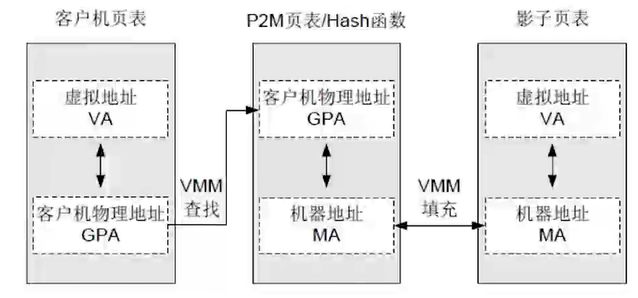
\includegraphics[]{cloud-memory-full-virtualization.png}
    \end{center}
\end{figure}


\subsubsection{内存半虚拟化技术}

通过使用页表写入法实现虚拟化。

Guest OS在创建一个新的页表时,会向VMM注册该页表。 之后在Guest运行的时候, VMM将不断的管理和维护这个表,使Guest上面的程序能直接访问到合适的地址。 

guest os直接向vmm注册, vmm跨层维护页表, virtual address直接翻译成physical address

\subsubsection{内存硬件辅助虚拟化技术}

通过扩展页表EPT (\term{extended page table})实现虚拟化。 

EPT通过使用硬件虚拟化技术,使其能在原有的页表的基础上,增加一个EPT页表,用于记录GPA到MA的映射关系。 VMM预先把EPT页表设置到CPU中。 

Guest修改Guest页表,无需VMM干预。 地址转换时, CPU自动查找两张页表完成Guest虚拟地址到机器地址的转换,从而降低整个内存虚拟化所需的开销。 

\begin{figure}[htbp]
    \begin{center}
        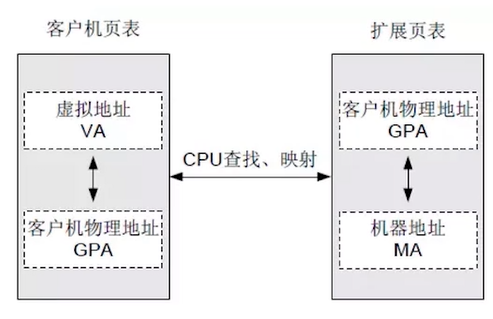
\includegraphics[]{cloud-memory-assisted-virtualization.png}
    \end{center}
\end{figure}

\subsection{I/O虚拟化技术}


\section{常见的虚拟化产品}

\begin{itemize}
    \item Hyper-V虚拟化
    \item Xen虚拟化
    \item Vmware虚拟化
    \item VirtualBox虚拟化
    \item KVM虚拟化
    \item Docker虚拟化
\end{itemize}


\section{容器}

\begin{definition}[容器]
    利用一个开源的容器引擎,让开发者可以打包他们的应用以及依赖包到一个可移植的镜像中,然后发布到任一Linux或Windows机器上,也可以实现虚拟化。 
\end{definition}

\begin{definition}[镜像]
    可执行的独立软件包,包含软件运行的内容:代码,运行时环境,系统工具,系统库和设置。 
\end{definition}

\begin{definition}[Docker]
    基于容器技术的\textbf{轻量级}虚拟化解决方案。 Docker是容器引擎,把Linux的cgroup、namespace等容器底层技术进行封装抽象,为用户提供了创建和管理容器的便捷界面(包括命令行和API)

\end{definition}

Docker作用:将应用程序与该程序的依赖,打包在一个文件里,运行这个文件,就会生成一个虚拟容器。 程序在这个虚拟容器里运行,就好像在真实的物理机上运行一样。 有了Docker,就不用担心环境问题[将程序和dependency包含在一个image中,使得对于全局配置的依赖解耦(应用和运行环境打包)]. 

\textbf{轻量级}的容器,可以只含有一个APP及其依赖。 base image包含OS等,APP image在base image之上

核心:实现应用与运行环境整体打包以及打包格式统一。 

Docker的好处

\begin{itemize}
    \item 秒级的交付和部署 $\rightarrow$ serverless依赖于轻量级容器技术,执行毫秒级高性能要求任务,重量级容器启动慢,轻量级只包含minimal set,deploy快;不定时的服务需求,需要尽快返回结果$\rightarrow$ 尽快部署, 如搜索服务
    \item 保证环境一致性
    \item 高效的资源利用
    \item 弹性的伸缩
    \item 动态调度迁移成本低
\end{itemize}

一个完整的Docker有以下几部分组成:
客户端(\term{Docker Client})、守护进程(\term{Docker Daemon})、镜像(\term{Docker Image})、容器(\term{Docker Container})、仓库(\term{Docker Registry})

\begin{figure}[htbp]
    \centering
    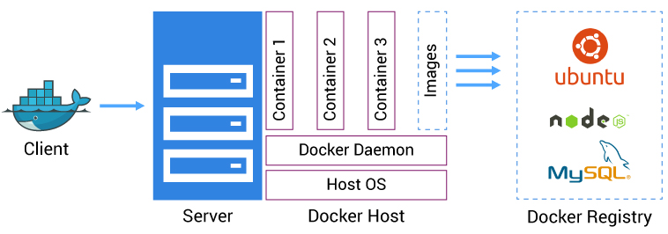
\includegraphics[width=\textwidth]{cloud-docker-architecture.png}
\end{figure}

Docker采用C/S架构,Docker Daemon作为服务端接受来自客户的请求,并处理这些请求(创建、运行、分发容器)。 客户端和服务端既可以运行在一个机器上,也可通过socket或者RESTful API来进行通信。 

Docker daemon一般在宿主主机后台运行,等待来自客户端的消息。 Docker客户端则为用户提供一系列可执行命令,用户用这些命令实现跟Docker daemon交互。 

\begin{figure}[htbp]
    \centering
    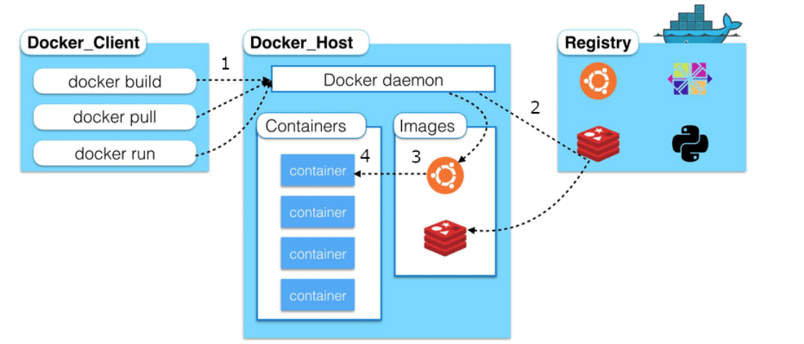
\includegraphics[width=\textwidth]{cloud-docker-architecture-2.png}
\end{figure}

\begin{definition}[Cluster]

\end{definition}

集群:基础运行收费(:只有运行时才能autoscale)+用户request多收费$\rightarrow$ 适用于中小企业

\begin{example}
    10 tasks:查询的数据库、代码等需先存入️集群中, 
当有新请求时,️自动部署新容器
\end{example}

集群由k8s管理,效率高; 有弹性; live migration成本低

\section{虚拟机与容器的对比}


\begin{figure}[htbp]
    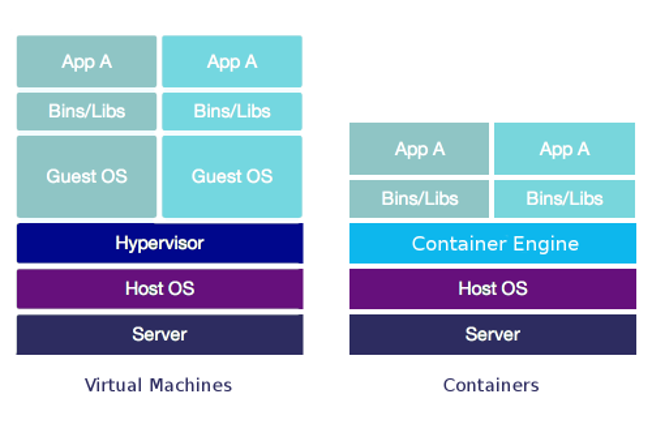
\includegraphics[width=\textwidth]{cloud-vmware-container-architecture.png}
\end{figure}

\begin{figure}[htbp]
    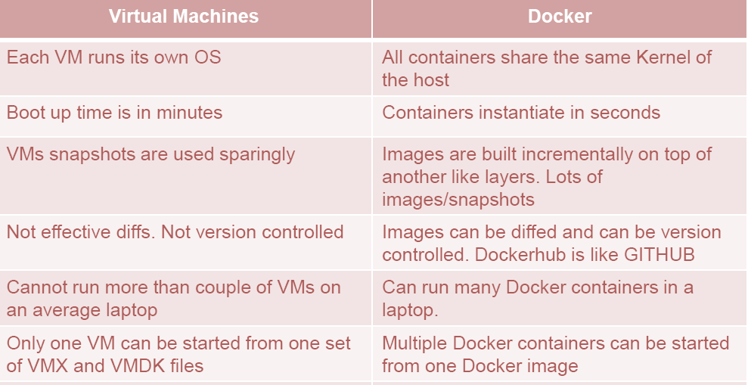
\includegraphics[width=\textwidth]{cloud-comparison-vmware-docker.png}
\end{figure}

\section{MapReduce, 并行}

\term{concurrent 并行}:同时进行

\term{(分时)并发}:2个任务同时发生,看似同时运行,但未必同时进行

\subsection{调度}

不同任务之间、不同io/网络等

MapReduce$\rightarrow$ Hadoop ,spark $\rightarrow$ spark的调度
\fi

\ifdefined\printdemo

\part{Example Codes}

%----------------------------------------------------------------------------------------
%	CHAPTER 1
%----------------------------------------------------------------------------------------

\chapterimage{chapter_head_2.pdf} % Chapter heading image

\chapter{Text Chapter}

\section{Paragraphs of Text}\index{Paragraphs of Text}

\lipsum[1-7] % Dummy text

%------------------------------------------------

\section{Citation}\index{Citation}

This statement requires citation \cite{article_key}; this one is more specific \cite[162]{book_key}.

%------------------------------------------------

\section{Lists}\index{Lists}

Lists are useful to present information in a concise and/or ordered way\footnote{Footnote example...}.

\subsection{Numbered List}\index{Lists!Numbered List}

\begin{enumerate}
\item The first item
\item The second item
\item The third item
\end{enumerate}

\subsection{Bullet Points}\index{Lists!Bullet Points}

\begin{itemize}
\item The first item
\item The second item
\item The third item
\end{itemize}

\subsection{Descriptions and Definitions}\index{Lists!Descriptions and Definitions}

\begin{description}
\item[Name] Description
\item[Word] Definition
\item[Comment] Elaboration
\end{description}

%----------------------------------------------------------------------------------------
%	CHAPTER 2
%----------------------------------------------------------------------------------------

\chapter{In-text Elements}

\section{Theorems}\index{Theorems}

This is an example of theorems.

\subsection{Several equations}\index{Theorems!Several Equations}
This is a theorem consisting of several equations.

\begin{theorem}[Name of the theorem]
In $E=\mathbb{R}^n$ all norms are equivalent. It has the properties:
\begin{align}
& \big| ||\mathbf{x}|| - ||\mathbf{y}|| \big|\leq || \mathbf{x}- \mathbf{y}||\\
&  ||\sum_{i=1}^n\mathbf{x}_i||\leq \sum_{i=1}^n||\mathbf{x}_i||\quad\text{where $n$ is a finite integer}
\end{align}
\end{theorem}

\subsection{Single Line}\index{Theorems!Single Line}
This is a theorem consisting of just one line.

\begin{theorem}
A set $\mathcal{D}(G)$ in dense in $L^2(G)$, $|\cdot|_0$. 
\end{theorem}

%------------------------------------------------

\section{Definitions}\index{Definitions}

This is an example of a definition. A definition could be mathematical or it could define a concept.

\begin{definition}[Definition name]
Given a vector space $E$, a norm on $E$ is an application, denoted $||\cdot||$, $E$ in $\mathbb{R}^+=[0,+\infty[$ such that:
\begin{align}
& ||\mathbf{x}||=0\ \Rightarrow\ \mathbf{x}=\mathbf{0}\\
& ||\lambda \mathbf{x}||=|\lambda|\cdot ||\mathbf{x}||\\
& ||\mathbf{x}+\mathbf{y}||\leq ||\mathbf{x}||+||\mathbf{y}||
\end{align}
\end{definition}

%------------------------------------------------

\section{Notations}\index{Notations}

\begin{notation}
Given an open subset $G$ of $\mathbb{R}^n$, the set of functions $\varphi$ are:
\begin{enumerate}
\item Bounded support $G$;
\item Infinitely differentiable;
\end{enumerate}
a vector space is denoted by $\mathcal{D}(G)$. 
\end{notation}

%------------------------------------------------

\section{Remarks}\index{Remarks}

This is an example of a remark.

\begin{remark}
The concepts presented here are now in conventional employment in mathematics. Vector spaces are taken over the field $\mathbb{K}=\mathbb{R}$, however, established properties are easily extended to $\mathbb{K}=\mathbb{C}$.
\end{remark}

%------------------------------------------------

\section{Corollaries}\index{Corollaries}

This is an example of a corollary.

\begin{corollary}[Corollary name]
The concepts presented here are now in conventional employment in mathematics. Vector spaces are taken over the field $\mathbb{K}=\mathbb{R}$, however, established properties are easily extended to $\mathbb{K}=\mathbb{C}$.
\end{corollary}

%------------------------------------------------

\section{Propositions}\index{Propositions}

This is an example of propositions.

\subsection{Several equations}\index{Propositions!Several Equations}

\begin{proposition}[Proposition name]
It has the properties:
\begin{align}
& \big| ||\mathbf{x}|| - ||\mathbf{y}|| \big|\leq || \mathbf{x}- \mathbf{y}||\\
&  ||\sum_{i=1}^n\mathbf{x}_i||\leq \sum_{i=1}^n||\mathbf{x}_i||\quad\text{where $n$ is a finite integer}
\end{align}
\end{proposition}

\subsection{Single Line}\index{Propositions!Single Line}

\begin{proposition} 
Let $f,g\in L^2(G)$; if $\forall \varphi\in\mathcal{D}(G)$, $(f,\varphi)_0=(g,\varphi)_0$ then $f = g$. 
\end{proposition}

%------------------------------------------------

\section{Examples}\index{Examples}

This is an example of examples.

\subsection{Equation and Text}\index{Examples!Equation and Text}

\begin{example}
Let $G=\{x\in\mathbb{R}^2:|x|<3\}$ and denoted by: $x^0=(1,1)$; consider the function:
\begin{equation}
f(x)=\left\{\begin{aligned} & {e}^{|x|} & & \text{si $|x-x^0|\leq 1/2$}\\
& 0 & & \text{si $|x-x^0|> 1/2$}\end{aligned}\right.
\end{equation}
The function $f$ has bounded support, we can take $A=\{x\in\mathbb{R}^2:|x-x^0|\leq 1/2+\epsilon\}$ for all $\epsilon\in\intoo{0}{5/2-\sqrt{2}}$.
\end{example}

\subsection{Paragraph of Text}\index{Examples!Paragraph of Text}

\begin{example}[Example name]
\lipsum[2]
\end{example}

%------------------------------------------------

\section{Exercises}\index{Exercises}

This is an example of an exercise.

\begin{exercise}
This is a good place to ask a question to test learning progress or further cement ideas into students' minds.
\end{exercise}

%------------------------------------------------

\section{Problems}\index{Problems}

\begin{problem}
What is the average airspeed velocity of an unladen swallow?
\end{problem}

%------------------------------------------------

\section{Vocabulary}\index{Vocabulary}

Define a word to improve a students' vocabulary.

\begin{vocabulary}[Word]
Definition of word.
\end{vocabulary}

%----------------------------------------------------------------------------------------
%	PART
%----------------------------------------------------------------------------------------

\part{Part Two}

%----------------------------------------------------------------------------------------
%	CHAPTER 3
%----------------------------------------------------------------------------------------

\chapterimage{chapter_head_1.pdf} % Chapter heading image

\chapter{Presenting Information}

\section{Table}\index{Table}

\begin{table}[h]
\centering
\begin{tabular}{l l l}
\toprule
\textbf{Treatments} & \textbf{Response 1} & \textbf{Response 2}\\
\midrule
Treatment 1 & 0.0003262 & 0.562 \\
Treatment 2 & 0.0015681 & 0.910 \\
Treatment 3 & 0.0009271 & 0.296 \\
\bottomrule
\end{tabular}
\caption{Table caption}
\label{tab:example} % Unique label used for referencing the table in-text
%\addcontentsline{toc}{table}{Table \ref{tab:example}} % Uncomment to add the table to the table of contents
\end{table}

Referencing Table \ref{tab:example} in-text automatically.

%------------------------------------------------

\section{Figure}\index{Figure}

\begin{figure}[h]
\centering
\includegraphics[scale=0.5]{placeholder.jpg}
\caption{Figure caption}
\label{fig:placeholder} % Unique label used for referencing the figure in-text
%\addcontentsline{toc}{figure}{Figure \ref{fig:placeholder}} % Uncomment to add the figure to the table of contents
\end{figure}

Referencing Figure \ref{fig:placeholder} in-text automatically.

\fi


%----------------------------------------------------------------------------------------
%	BIBLIOGRAPHY
%----------------------------------------------------------------------------------------
\printbibliography

% For print bibliography according to their type,
% For unknown reasons, this does not work.

%\chapter*{Bibliography}
% \addcontentsline{toc}{chapter}{\textcolor{ocre}{Bibliography}} % Add a Bibliography heading to the table of contents



% For print bibliography according to their type,
% For unknown reasons, this does not work.
%------------------------------------------------


% \section*{Articles}
% \addcontentsline{toc}{section}{Articles}
% \printbibliography[heading=bibempty,type=article]

%------------------------------------------------

% \section*{Books}
% \addcontentsline{toc}{section}{Books}
% \printbibliography[heading=bibempty,type=book]

%----------------------------------------------------------------------------------------
%	INDEX
%----------------------------------------------------------------------------------------

\cleardoublepage % Make sure the index starts on an odd (right side) page
\phantomsection
\setlength{\columnsep}{0.75cm} % Space between the 2 columns of the index
\addcontentsline{toc}{chapter}{\textcolor{ocre}{Index}} % Add an Index heading to the table of contents
\printindex % Output the index



%----------------------------------------------------------------------------------------

\end{document}
